%The following line prevents the headers and the \begin{document}\end{document}
%from being executed in the individual files.
\def\whole{}
\documentclass[leqno]{book}
%\usepackage{msribib,local}
\input style-for-curves.sty
\usepackage{hyperref}
\usepackage{msribib}
\usepackage{pdfpages}
%\input header.tex

%\documentclass{cambridge7A}
%\usepackage{ag2}
\usepackage{xcolor}
%\usepackage{mtpro2}
%\usepackage{times}
%\usepackage{hatcher}
%\usepackage{msribib,local}
%\usepackage{geompsfi}

\errorcontextlines=1000

%\usepackage{makeidx}
\makeindex
% \index{word} in the doc; \index{variety!algebraic} gives variety, algebraic
% PUT a % after each \index{***}

\overfullrule=5pt
\catcode`\@\active
\def@{\mskip1.5mu} %produce a small space in math with an @

\title{Personalities of Curves}
\author{\copyright David Eisenbud and Joe Harris}

%\includeonly{12-HilbertSchemes, 13-HilbertSchemesII }
%\def\all{toc,out1,chern,out2,lefschetz,out3,bib,ind, out1a}
%\includeonly{\all}

\begin{document}
\maketitle

\pagenumbering{roman}
\setcounter{page}5
\pagenumbering{arabic}
\tableofcontents

\input header.tex

\setcounter{chapter} {-1}
\chapter{Basic Questions}

\fix{The following is more material for a preface than a preface...}
\begin{center}
\emph{I'm very well acquainted, too, with matters mathematical,\\
I understand equations, both the simple and quadratical,\\
About binomial theorem I am teeming with a lot o' news,\\
With many cheerful facts about the square of the hypotenuse.}

---Gilbert and Sullivan, Pirates of Penzance, Major General's Song


\emph{Be simple by being concrete. Listeners are prepared to
accept unstated (but hinted) generalizations much more than they are able, on the spur of the moment, to
decode a precisely stated abstraction and to re-invent the special cases that motivated it in the first place. }

--Paul Halmos, How to Talk Mathematics

\emph{Another damned thick book! Always scribble, scribble, scribble! Eh, Mr. Gibbon?} --- \scriptsize{Prince William Henry, upon receiving the second  volume of The History of the Decline and Fall of the Roman Empire from the author.}
\end{center}


The most primitive objects of algebraic geometry are affine algebraic sets---subsets of $\RR^{n}$ or $\CC^{n}$ defined by the vanishing of polynomial functions---and the maps between them. But already in the first half of the 19th century geometers realized that there was a great advantage in working with varieties in complex projective space, treating affine varieties as projective varieties minus the intersection with the plane at infinity and real varieties as the fixed points of the complex involution. One sees this in the simplest examples: the ellipses, hyperbolas and parabolas in the real affine plane are all the same in the complex projective plane; the difference is only in how they intersect the line at infinity. A difficulty with the projective point of view is that on a connected projective variety there are no non-constant functions at all (reason: a function on a projective variety is a map to the affine line; since the image of a projective variety is again projective, the image would be a single point.) 

Starting with Riemann in the 1860s and culminating in the scheme theory of Grothendieck in the 1950s, algebraic varieties were treated in a way independent of any embedding: An algebraic variety is is a topological space with a sheaf of locally
defined polynomial functions. Many interesting aspects of geometry have to do not with single abstract varieties, but with maps between them, and in particular with embeddings in projective spaces. In general, maps between varieties can be described by their graphs, which are again varieties.  But for the special case of maps to projective spaces, the theory of \emph{linear series} is usually a more convenient description. The collection of all linear series on a variety reflects some of its best understood invariants. 

The basic objects of study in this book are smooth, connected projective algebraic curves over an algebraically closed field of characteristic 0, which we take to be the complex numbers $\CC$. Though we assume that the reader has been exposed to this theory in some form before, perhaps from Chapter IV of Hartshorne's {\it Algebraic Geometry}, we will review the elements  in the form we will use. 

\section{Algebraic Curves and Riemann Surfaces}

These objects can be viewed in two distinct but equivalent ways: as \emph{compact Riemann surfaces}, or compact complex manifolds of dimension 1; and as \emph{smooth projective algebraic curves over $\CC$}. (Here, when we use the term projective variety, we mean a variety isomorphic to a closed subset of projective space, not a variety with a specified embedding in $\PP^n$.) There are advantages to each point of view---the complex analytic point of view is more concrete, and requires relatively minimal amount of preliminaries; the algebraic point of view is substantially broader. 

First, if $C \subset \PP^n$ is a smooth, projective curve over $\CC$, then it is a submanifold of complex projective space, and so a Riemann surface. 
\fix{discuss geometric genus vs. arithmetic genus here?}

The other direction---going from a compact Riemann surface $C$ to a smooth projective curve over $\CC$, or equivalently embedding $C$ as a complex submanifold of $\PP^n$, after which Chow's theorem says that it is in fact a projective variety---is much deeper. The first, and hardest step is to show that a compact Riemann surface admits a nonconstant meromorphic function $f:C \to \CC$, and the corresponding statement is not true in higher dimensions. The function $f$ can be viewed as
a rational map $f': C\to \PP^{1}$. The next step is to see that the field $K(C)$ of all meromorphic functions
on $\CC$ is a finite extension of the field of rational functions on $\PP^{1}$; the sheaf of regular functions on $C$ is then the integral closure of the sheaf of regular functions on $\PP^{1}$ in $K(C)$.

Though equivalent for curves defined over $\CC$, these approaches have a very different flavors. For example,
given a map  $f: C\to C'$ from a smooth curve $C$ to a possibly singular curve $C'$ that is generically one-to-one, we can reconstruct $C$.
From the algebraic point of view this can be done by \emph{normalization}, or more concretely by blowing up the singular points of $C'$. From the analytic point of view, we can use the Weierstrass preparation theorem, which implies that there is the neighborhood $U$ of any point $p\in C'$ such that the punctured neighborhood $U \setminus p$ is isomorphic to a disjoint union of punctured discs; and $C$ is obtained by completing this to the corresponding disjoint union of discs.

\section{Families of varieties}

\subsection{Hilbert schemes}

\subsubsection{Definition, universal property; construction}

\subsubsection{examples of hypersurfaces and linear spaces}

\subsubsection{tangent space}

\subsubsection{Fundamental problem: irreducible components of Hilb parametrizing smooth curves and their dimensions}

\begin{example}
conics in $\PP^3$ (refer to 3264)
\end{example}

\subsection{Moduli spaces of curves}

\subsubsection{basic properties of $M_g$ (coarse rather than fine; fine over automorphism-free curves)}

\subsubsection{dimension $3g-3$, irreducible}  (just statements, w/ref to Harris-Morrison)



\section{Moduli problems}

It is a fundamental aspect of algebraic geometry that the objects we deal with often vary in families, and can often be parametrized by a ``universal" such family. For example, the family of plane curves of degree $d$ may be thought of as the projective
space $\PP(H^{0} \sO_{\PP^{2}}(d))$, and similarly with hypersurfaces in any projective space. This notion of objects varying with parameters underlies many of the constructions and theorems we will discuss. 

\subsection{What is a moduli problem?}

Briefly, a \emph{moduli problem} consists of two things: a class of objects, or isomorphism classes of objects; and a notion of what it means to have a \emph{family} of these objects parametrized by a given scheme $B$. To make this relatively explicit, the four main examples of moduli problems we'll be discussing here are:

\begin{enumerate}
\item  smooth curves: objects are isomorphism classes  of smooth, projective curves $C$ of a given genus $g$. A family over $B$ is a subscheme $\cX \subset B \times \PP^r$, smooth, over $B$, whose fibers are curves of genus $g$.

\item the Hilbert scheme: objects are subchemes of $ \PP^r$ with a given Hilbert polynomials. A family  is a subscheme $\cX \subset B \times \PP^r$, with $cX$ flat over $B$, whose fibers have the given Hilbert polynomial. We will be interested in the case of Hilbert polynomial $p(m) = dm-g+1$ and the open subscheme corresponding to smooth projective curves $C \subset \PP^r$ of degree $d$ and genus $g$.

\item effective divisors on a given curve: objects are effective divisors of a given degree $d$ on a given smooth, projective curve $C$. A family over $B$ will be a subscheme $\cD \subset B \times C$ flat over $B$, with fibers of degree $d$

\item invertible sheaves on a given curve $C$: objects are invertible sheaves of a given degree $d$ on $C$. A family over $B$ is an invertible sheaf on the product $B \times C$ whose restriction to each fiber over $B$ has degree $d$. We identify two such sheaves if they differ by tensor product with an invertible sheaf pulled back from $B$.
\end{enumerate}

Given a moduli problem, our goal will be to describe a corresponding \emph{moduli space}. By this we mean a scheme $M$ whose points are in \emph{natural} one-to-one correspondence with the objects in our moduli problem. This will realize the objects of the moduli problem as the points of the underlying set of the scheme $M$.

If the moduli space in question and the base of the family are varieties, then the crucial condition that the correspondence be \emph{natural} is simple to express: that given a family of the objects in our moduli problem over a variety $B$, the map from underlying set of $B$ to the underlying set of $M$ taking each fiber
to the corresponding point of $M$ should be a morphism of varieties.  But in the world of schemes the set-theoretic mapping does not determine the morphism of schemes (think, for example, of the morphisms from $\Spec(\CC[x]/x^{2})$ into the plane with the closed point mapping to the origin. The situation is even worse when the moduli space itself is not a variety.)

To deal with the general case, we recast the naturality condition in functorial terms. We observe first that a moduli problem defines a functor $\cM$ from the category of schemes to the category of sets: the value of the functor at a scheme $B$ is the set of families of objects parametrized by $B$; a morphism $B' \to B$ of schemes gives rise, via pullback, to a map of sets $\cM(B) \to \cM(B')$. We define a \emph{fine moduli space} for the moduli problem to be a scheme $M$ that represents this functor, in the sense that there is an isomorphism of functors
$$
\cM \to {\rm Mor}(\bullet, M)
$$
In other words, for every scheme $B$ we have a bijection between families of our objects over $B$ and morphisms from $B$ to $M$. In particular, applying this to $B = \Spec \CC$, we have a bijection between the set of objects and the closed points of $M$; and for any family over an arbitrary scheme $B$, the map from $B(\CC)$ to $M(\CC)$ sending each closed point  $b \in B$ to the point in $M(\CC)$ corresponding to the fiber over $b$ is the underlying map of a morphism $B \to M$ of schemes.

If a fine moduli space for a given problem exists at all, then Yoneda's Lemma shows that it is unique up to a unique isomorphsm. This is a real problem: there is no fine moduli space for the first and most important of the examples above---the isomorphism classes of smooth curves---though there is for the others. We'll defer the discussion of why this is, and what we can do about it, until Chapter~\ref{Moduli chapter}.

Looking ahead, we'll discuss the third and fourth example in Chapter~\ref{}, where we'll describe the moduli spaces for effective divisors of given degree $d$ on a given curve $C$ (the symmetric powers of the curve) and for invertible sheaves of a given degree on $C$ (the \emph{Jacobian} and \emph{Picard variety} of $C$). These, as we'll see, are smooth, irreducible projective varieties of dimensions $d$ and $g$ respectively.

We'll take up the moduli space $M_g$ of smooth curves in Chapter~\ref{Moduli chapter}, where we'll see that this space (or rather the closest approximation to it we can cook up) is irreducible of dimension $3g-3$ for $g \geq 2$, though not smooth or projective.

Finally, the Hilbert scheme will be described (to the extent that we can!) in Chapter~\ref{HilbertSchemesChapter}; this will turn out to be much wilder and more varied in its behavior than any of the above.




%\section{Outline}
% \begin{enumerate}
%
%\item Background \begin{enumerate}
%
%\item Lasker's Theorem (complete intersections are unmixed) -- sometimes incorrectly called ``$AF+BG$''
%state ci implies unmixed; prove by $H^1$ of line bundle.
%
%\item B\'ezout and the  weak B\'ezout (ex 8.4.6 in Fulton).
%B\'ezout via Koszul complex, at least in codim 2.
%
%
%
%
%\end{enumerate}
%\item Basics of curves (corresponds to material in Hartshorne Ch 4, sects 1,2,4(?)---all except elliptic curves and ``classification")
%
%\begin{enumerate}
% \item Discussion of genus of smooth curves. Riemann-Roch. Hilbert coefficient.
%
%\item Divisors and maps; canonical divisor -- cotangent bundle; canonical map as example
%Exercise: Projections from on and off a curve
%
%\item canonical series is bpf, $2g+1$ is very ample. Canonical Curves and geometric RR
%
%\item Adjunction formula for curves in a surface (Quote from Hartshorne)
%
%\item Clifford, including strong form, canonical series is va except in hyperelliptic case.
%
%\item Riemann-Hurwitz (pull back a differential form)
%
%\end{enumerate}
%%\end{enumerate}
%
%\item Families of curves and Brill-Noether theory
%\begin{enumerate}
%\item Families. Define families. discuss "good and bad" families. example: symmetric product. example: plane curves of degree d. family of line bundles on a curve (or a family of curves.)
%
%\item How many curves of genus g are there? Informal discussion of moduli. 
%\item Cheerful fact about the existence of  Hilbert scheme, $M_g$, and $\overline M_g$, meaning of the phrase ``coarse moduli space''.
%
% \item Lowest degree of a covering of $\PP^1$?
% \item Lowest degree of a plane model?
% \item Lowest degree of an embedding?
% \item Number of forms of of degree d vanishing on the curve---ideals of the embeddings, Hilbert Functions.
%\end{enumerate}
%
%\item Personalities
%\begin{enumerate}
%\item $g=0$: rational curves as projections of rational normal curves. Rational quartic in $\PP^3$. Mention Set-Theoretic Complete Intersection problem.
%\item $g=1$. Wonderful subject; refer to somewhere else. Plane cubic, quartic in $\PP^3$, state that an elliptic quintic is Pfaffian (give proof??).
%\item $g=2$. Canonical map to $\PP^1$. Embedding in $\PP^3$ as $(2,3)$ on a quadric, ideal is 1 quadric, 2 cubics.
%\item $g=3$. Plane quartics. Sextic curves in $\PP^3$: general $g^3_6$ is an embedding, det variety.  $g\times g+1$ matrix of linear forms in $\PP^3$ gives curve of genus $g$, degree ${g\choose 2}$
%\item $g=4$. Canonical model is ci. Therefore $C$ is a 3-sheeted cover of $\PP^1$, in 1 or 2 ways, depending on the singularity of the unique quadric in the ideal.
%\item $g=5$. Canonical model lies on 3 quadrics. Either a CI, or trigonal. In latter case, Pfaffians. Introduce Green's conjecture?
%\item $g=6$. Canonical model lies on at least 6 quadrics. We will see exactly 6, and what they are...(projective normality of canonical embedding; and Brill-Noether for the plane model with 4 nodes.) Talk about the del Pezzo.
%\end{enumerate}
%
%\item Abel map and Jacobian
%\begin{enumerate}
%\item $J = H^0(\omega)^\vee/\hbox{lattice of periods}$. $\dim J = g$ general $g^3_{g+3}$ is very ample. Do this as an example of Hodge Theory.
%
%\item Symmetric powers, Abel-Jacobi map, Abel's Theorem (statement), differential of the Abel map.
%\item connection with addition formulas for integrals
%\end{enumerate}
%
%\item Scrolls, Hyperelliptic curves, trigonal curves 
%\begin{enumerate}
%\item general emb of degree $g+3$, in $\PP^3$ as divisor on a quadric of type $(2,g+1)$
%\item Other linear series on hyperell curve: 1) special linear series are mult $g^1_2$+basepoints. 2) Given an embedding, there's a union of lines. If the embedding is complete, we get a matrix...that defines the union of lines. Scrolls in all dimensions as unions of spans of divisors. 
%\item scrolls, starting with the matrix. Map to $\PP^1$ is the line bundle defined by the cokernel. Get the VB as the pushforward of $\cO(1)$.
%Mention higher-dim scrolls, but do surface scrolls in more detail: dim and genus of curves in each linear series. Condition for the existence of integral curves in each class iff the int number with the directrix is >0 and the curve is not a multiple of the fiber. 
%\item Minimal degree varieties; as the varieties of given degree lying on the maximal number of quadrics. 
%\item Type of scroll containing a hyperelliptic curve (Maroni invariant) --- invariant of the line bundle
%\item canonical image of a trigonal curve lies on a 2-dim scroll (non -subcanonical embedding only on 3-dim scrolls).  embedding of a trigonal curve lies on the same scroll.Stratification of trigonal curves by Maroni invariants. Dimensions via automorphism groups of scrolls.
%\item for a curve of genus 5, not cut out by quadrics:
% the intersection of the quadrics containing $C$ is two-dimensional: a rational normalscroll;  and  $C$ is trigonal, that is, a 3-sheeted cover of $\PP^1$. 
%\item Statement of Castelnuovo theory
%
%\item Old list: Scrolls and their divisors
%\begin{enumerate}
% \item Hirzebruch surfaces embedded by complete series
% \item lines joining 2 rational normal curves
% \item determinantal varieties
%\end{enumerate}
%
%\end{enumerate}
%
%\bigbreak

%\centerline {\bf Appendices?}
%\item Castelnuovo Theory
%\begin{enumerate}
%\item Ineq on Hilbert functions, leading to bound on $g,d$. 
%\item Give the scroll examples
%\item Castelnuovo's lemma (2n+3 points in $\PP^n$ by determinantal proof) 
%\item Characterization of Castelnuovo curves
%\item Projective normality of the canonical curve.
%\end{enumerate}

%\item Parameter space (open problems to be discussed in BN chapter or following.
%\begin{enumerate}
%\item Survey: Hilbert Scheme, Hurwitz Variety, Moduli
%\item Irreducibility (or not) and dimension. 
%\end{enumerate}
%
%\item Projective Normality
%\begin{enumerate}
%\item Castelnuovo's theorem: $2g+1$ is projectively normal.
%\item Liaison of curves in $\PP^3$.
% \end{enumerate}
%
%
%\item Inflectionary behavior and Brill-Noether
%\begin{enumerate}
% \item Pl\"ucker formulas
% \item Weierstrass Points
% \item finiteness of the automorphism group
%\item Proof of 1/2 BN by cuspidal curves
%\item Reference to the appendix of 3264 for the existence half
%\item generic $g^2_*$ is birational; $g^3_*$ is very ample (on a general curve)
%\end{enumerate}
%
%
%
%
%%\item
%%\begin{enumerate}
%%\item Broader View: 
%%\end{enumerate}
%
%
%
%\end{enumerate}
%


\begin{thebibliography}{ABC99}

%\bibitem[1965]{BR} D. Buchsbaum and D.S.Rim.
%A generalized Koszul complex. III. A remark on generic acyclicity.
%Proc. Amer. Math. Soc. 16 (1965) 555--558. 

\bibitem[Walker]{Walker} Walker.
\bibitem[Hartshorne]{Hartshorne} Hartshorne Ch 4
\bibitem[Fulton]{Fulton} Fulton Alg curves
\bibitem[Schemes]{Eisenbud-Harris} Schemes
\bibitem[3264]{Eisenbud-Harris} 3264
\bibitem[Griffiths-Harris]{Griffiths-Harris} (for the Abel-Jacobi stuff)
\bibitem[Griffiths]{Griffiths-Chinese}(for the Abel-Jacobi stuff)
\bibitem[Mumford]{Mumford}-Curves and their Jacobians
\bibitem[Voisin]{Voisin} Hodge Theory
%\bibitem[]{Smith} Smith, K.

\end{thebibliography}
\bigskip

\vbox{\noindent Author Addresses:\par
\smallskip
\noindent{David Eisenbud}\par
\noindent{Department of Mathematics, University of California, Berkeley,
Berkeley CA 94720}\par
\noindent{eisenbud@math.berkeley.edu}\par
}

\input footer.tex
%header and footer for separate chapter files

\ifx\whole\undefined
\documentclass[12pt, leqno]{book}
\usepackage{graphicx}
\input style-for-curves.sty
\usepackage{hyperref}
\usepackage{showkeys} %This shows the labels.
%\usepackage{SLAG,msribib,local}
%\usepackage{amsmath,amscd,amsthm,amssymb,amsxtra,latexsym,epsfig,epic,graphics}
%\usepackage[matrix,arrow,curve]{xy}
%\usepackage{graphicx}
%\usepackage{diagrams}
%
%%\usepackage{amsrefs}
%%%%%%%%%%%%%%%%%%%%%%%%%%%%%%%%%%%%%%%%%%
%%\textwidth16cm
%%\textheight20cm
%%\topmargin-2cm
%\oddsidemargin.8cm
%\evensidemargin1cm
%
%%%%%%Definitions
%\input preamble.tex
%\input style-for-curves.sty
%\def\TU{{\bf U}}
%\def\AA{{\mathbb A}}
%\def\BB{{\mathbb B}}
%\def\CC{{\mathbb C}}
%\def\QQ{{\mathbb Q}}
%\def\RR{{\mathbb R}}
%\def\facet{{\bf facet}}
%\def\image{{\rm image}}
%\def\cE{{\cal E}}
%\def\cF{{\cal F}}
%\def\cG{{\cal G}}
%\def\cH{{\cal H}}
%\def\cHom{{{\cal H}om}}
%\def\h{{\rm h}}
% \def\bs{{Boij-S\"oderberg{} }}
%
%\makeatletter
%\def\Ddots{\mathinner{\mkern1mu\raise\p@
%\vbox{\kern7\p@\hbox{.}}\mkern2mu
%\raise4\p@\hbox{.}\mkern2mu\raise7\p@\hbox{.}\mkern1mu}}
%\makeatother

%%
%\pagestyle{myheadings}

%\input style-for-curves.tex
%\documentclass{cambridge7A}
%\usepackage{hatcher_revised} 
%\usepackage{3264}
   
\errorcontextlines=1000
%\usepackage{makeidx}
\let\see\relax
\usepackage{makeidx}
\makeindex
% \index{word} in the doc; \index{variety!algebraic} gives variety, algebraic
% PUT a % after each \index{***}

\overfullrule=5pt
\catcode`\@\active
\def@{\mskip1.5mu} %produce a small space in math with an @

\title{Personalities of Curves}
\author{\copyright David Eisenbud and Joe Harris}
%%\includeonly{%
%0-intro,01-ChowRingDogma,02-FirstExamples,03-Grassmannians,04-GeneralGrassmannians
%,05-VectorBundlesAndChernClasses,06-LinesOnHypersurfaces,07-SingularElementsOfLinearSeries,
%08-ParameterSpaces,
%bib
%}

\date{\today}
%%\date{}
%\title{Curves}
%%{\normalsize ***Preliminary Version***}} 
%\author{David Eisenbud and Joe Harris }
%
%\begin{document}

\begin{document}
\maketitle

\pagenumbering{roman}
\setcounter{page}{5}
%\begin{5}
%\end{5}
\pagenumbering{arabic}
\tableofcontents
\fi


\chapter{Lasker's and B\'ezout's Theorems}

\section{The Noether-Lasker-Macaulay Theorems}

A key element in the algebraic study of plane curves initiated by Brill and Noether following Riemann's discoveries was what Noether named the ``Fundamental Lemma on Holomorphic Functions.'' In the original language it said that if the homogeneous forms $F(x_{0},x_{1},x_{2})=0$ and $G(x_{0},x_{1},x_{2})=0$ are the equations of two curves in $\PP^{2}$ that have no component in common, then any form $H$ that locally represents a function (the ``holomorphic functions'' of the name) vanishing on all the points
of the intersection must have an expression $H = AF+BG$, where $A,B$ are also homogeneous forms. It was extended by Lasker to the case of many polynomials (homogeneous or not) in many variables. (This is sometimes called the ``$AF+BG$ Theorem''.) 

\begin{theorem}\label{Lasker}
Suppose that $I = (f_{1}, \dots, f_{c}) \subsetneq S:=\CC[x_{0},\dots,x_{n}]$ is an ideal generated by $c$ homogeneous forms in a polynomial ring. 
The scheme $X:= V(I)$ is either empty or has codimension $\leq c$. If equality holds, then
\begin{enumerate}
 \item Every primary component of $I$ has codimension exactly $c$; in particular, if $c<n+1$ then $I$ is saturated.
 \item $\HH^{i}(\cO_{X}(d)) = 0$ for all $0<i<\dim X$ and all $d\in \ZZ$.
 \item If $\dim X\geq 1$
then the map
$\HH^{0}(\cO_{\PP^{n}}(d)) \to \HH^{0}(\cO_{X}(d))$ is surjective for every $d$.
\end{enumerate}
\end{theorem}

By the Principal Ideal Theorem(\cite[Theorem ***]{Eisenbud95} the codimension of $V(f_{1},\dots, f_{c})$ is at most $c$;
the Theorem thus covers the case where the codimension is ``as large as possible'', that is, the $V(f_{i})$ meet eachother
in a dimensionally transverse way.

In modern language, the conclusion says that the ring $S/I$ is Cohen-Macaulay. See for example \cite[Chapter 18]{Eisenbud95}, where the result it proven in greater generality.

Theorem~\ref{Lasker} immediately implies the orginal version of the theorem because (by the Nullstellensatz) the set of forms vanishing on $V(f_{1}, \dots, f_{c})$ is the saturation 
of the ideal $(f_{1}, \dots, f_{c})$. 

We will make use of the following algebraic Lemma, proven in  in \cite[Theorem 18.***]{Eisenbud95}:

\begin{lemma}\label{Cohen-Macaulay}
 Under the hypothesis of Theorem~\ref{Lasker}, the polynomial $f_{i}$ is a nonzerodivisor in the ring 
$S/(f_{1}, \dots, f_{i-1})$ for $i = 1, \dots, c$.
\end{lemma}

The conclusion is usually stated by saying that   $f_{1}, \dots, f_{c}$ is a \emph{regular sequence}.

\begin{proof}[Partial Proof]
 The result is obvious for $c=1$. For $c=2$ the hypothesis implies that $f_{1}$ and $f_{2}$ have no common factor.
If $g f_{2} \equiv 0\ {\rm mod}\ f_{1}$ then, since $S$ has unique prime factorization, $g$ must be divisible by
$f_{1}$, that is, $g  \equiv 0\ {\rm mod}\ f_{1}$, proving the result for $c=2$. In general, the result is equivalent to the 
statement that $S$ is a Cohen-Macaulay ring,  \cite[Proposition 18.9]{Eisenbud95}.
\end{proof}


\begin{proof} [Proof of Theorem~\ref{Lasker}] We do induction on $c$. For $c=0$ the saturation is trivial, and the vanishing in the case $c=0$ is the usual computation of the cohomology of line bundles on $\PP^{n}$. 

Now suppose that the theorem is true for $X' := (f_{1}, \dots f_{c-1})$. Note that $\dim X' = n-c+1\geq 1$.
 The surjectivity of 
the maps $\HH^{0}(\cO_{\PP^{n}}(d)) \to \HH^{0}(\cO_{X'}(d))$ shows that the homogeneous coordinate ring
of $X'$ is $R':=\oplus_{d} \HH^{0}(\cO_{X'}(d))$.

Write $e$ for the degree of $f_{c}$ . By Lemma~\ref{Cohen-Macaulay} there is a short
exact sequence
$$
0\to \cO_{X'}(-e) \rTo^{f_{c}} \cO_{X'} \to \cO_{X} \to 0.
$$
Tensoring with $\cO_{\PP^{n}}(d)$, and passing to cohomology, we obtain a long exact sequence that begins
\begin{align*}
0\to &\HH^{0}(\cO_{X'}(d-e_{1})) \rTo^{f_{1}}  \HH^{0}(\cO_{X'}(d)) \to  \HH^{0}(\cO_{X}(d))\to\\
&\HH^{1}(\cO_{X'}(d-e_{1}))\to \cdots .
\end{align*}
From the exactness of the top row we see that every element of $R$ 
that vanishes on $X$ is a multiple of $f_{c}$, so $f_{c}$ generates the homogeneous ideal of $X$ in $R$.
Lifting this back to the polynomial ring and using
 the inductive hypothesis, we see that $f_{1},\dots, f_{c}$ generate the homogeneous ideal of
$X$ in $S$.

Moreover, if $\dim X\geq 1$ then $\dim X' \geq 2$, so $\HH^{1}(\cO_{X'}(d-e_{1})) = 0$ for all $d$ by the induction,
whence the surjectivity statement holds for $X$.

Finally, the induction hypothesis and the exact sequences
$$
\HH^{i}(\cO_{X'}(d)) \to  \HH^{i}(\cO_{X}(d))\to \HH^{i+1}(\cO_{X'}(d-e_{1}))
$$
together show that $\HH^{i}(\cO_{X}(d)) = 0$ for $i<\dim X = \dim X'-1$.

\end{proof}

\subsection{Determinantal ideals}
There is a natural generalization of Theorem~\ref{Cohen-Macaulay} that will be useful to us in constructing the 
ideals of embedded curves.  Consider a homomorphism
$$
\bigoplus_{j=1}^{q}\cO_{\PP^{n}}(d_{j}) \rTo^{M}
\bigoplus_{i=1}^{p}\cO_{\PP^{n}}(e_{i})
$$
given by a 
 $p\times q$ matrix of forms
$$
M:=\begin{pmatrix}
 f_{1,1}&f_{1,2}&\dots&f_{1,q}\\
\vdots&&\ddots&\vdots\\
f_{p,1}&f_{p,2}&\dots&f_{p,q}\\
\end{pmatrix}
$$
with $\deg f_{i,j} = \delta_{i,j} := e_{i}-d_{j}$. 

When $p=1$, this is just a sequence of forms of the type considered
in Theorem~\ref{Cohen-Macaulay}. 

\begin{theorem} (Macaulay)\label{determinantal Cohen-Macaulay}
Suppose $p\leq q$, and let $I$ be the ideal of $p\times p$ minors of the matrix $M$.
The scheme $X:= V(I)$ is either empty or has codimension $\leq c:= q-p+1$. If equality holds,  then 
\begin{enumerate}
 \item Every primary component of $I$ has codimension exactly $c$; in particular, if $c<n+1$ then $I$ is saturated.
 \item $\HH^{i}(\cO_{X}(d)) = 0$ for all $0<i<\dim X$ and all $d\in \ZZ$.
 \item if $\dim X\geq 1$
then the map
$\HH^{0}(\cO_{\PP^{n}}(d)) \to \HH^{0}(\cO_{X}(d))$ is surjective for every $d$.
\end{enumerate}
\end{theorem}

See *** for a proof.

\begin{fact}
There are further theorems of this type, for lower order minors, for symmetric matrices, for skew symmetric matrices, etc. Perhaps the most general
statement is that if $R$ is a regular local ring and $R/J$ is a Cohen-Macaulay ring then if $\phi:R\to S$ is a local homomomorphism to a Cohen-Macaulay ring, then $\codim JS\leq \codim J$ and, if equality holds then
$S/IS$ is Cohen-Macaulay. For example, Theorem~\ref{Cohen-Macaulay} may be regarded as the case where
$R$ is a polynomial ring in $c$ variables, and $J$ is the ideal generated by the variables. See for example~\cite{Jee Koh, Super Height paper}.
\end{fact}

\section{B\'ezout's Theorem}

The most basic invariants of a subvariety $X$ of $\PP^{n}$ are its dimension and degree; for example, they determine its cohomology class in the integral cohomology $\HH^{*}(\PP^{n}; \ZZ) \cong \ZZ[x]/(x^{n+1})$.  It is convenient to compute these invariants in the case of schemes using the Hilbert polynomial. It is convenient that this definition extends at once to coherent sheaves:

\begin{theorem}
 Let $X\subset \PP^{n}$ be a subscheme. The function
 $P_{X}(t): = \chi(\cO_{X}(t)$
 is a polynomial whose degree is equal to the dimension of $X$ and whose leading coefficient
is $\deg X/(\dim X)!$. 
\end{theorem}

\begin{proof}
 We do induction on the dimension. If the dimension of $X$ is zero, then $\cO_{X}$ has a composition series
 whose successive factors have the form $\cO_{p}$, for various points $p\in \PP^{n}$, and the number of these points
 is the degree of $X$. By the additivity of the Euler characteristic, it suffices to prove the formula for a single point $p$.
 But $\cO_{p}(t) \cong \cO_{p}$, while $\HH^{0}(\cO_{p}) = 1$ and $\HH^{i}\cO_{p} = 0$. Thus 
 $\chi(\cO_{p}(t)) = 1$ for all $t$, as required.
 
 Now suppose $\dim X\geq 1$. If
 If $x$ is a general linear form on $\PP^{n}$ then $x$ is a non-zerodivisor on 
 $\cO_{X}$. Let $H$ be the hyperplane defined by $x$. Then $X' = X\cap H$ has the same degree as $X$, and dimension
 1 less. Twisting the exact sequence
 $$
 0\to \cO_{X}(-1) \to \cO_{X} \to \cO_{X'} \to 0
 $$
 by $\cO_{\PP^{n}}(t)$ we see that 
 $$
\chi(\cO_{X'}(t)) =  \chi(\cO_{X}(t)) - \chi(\cO_{X}(t-1)).
 $$
so the degree of $\chi(\cO_{X'}(t)$ is one less than the degree of $\chi(\cO_{X'}(t)$, and the leading coefficient
of $\chi(\cO_{X'}(t)$ is $\dim X$  times the leading coefficient of $\chi(\cO_{X}(t)$
\end{proof}

For example, $\PP^{n}$ itself has degree 1 since 
$$
\chi(\cO_{\PP^{n}}(t)) = {n+t\choose n} = \frac{t^{n}}{n!} +\hbox{lower degree terms}.
$$
Also, a hypersurface defined by a form of degree $d$ does indeed have degree $d$---otherwise we would not have made
this definition! More generally:

\begin{lemma}\label{nzd Bezout}
Let $X\subset \PP^{n}$ be a subscheme, and suppose that $f \in \HH^{0}(\cO_{\PP^{n}}(d))$ is form of degree $d$. Let $H$ be the hypersurface $V(f)$.  If
the induced map $\cO_{X}(-d) \to \cO_{X}$ is a monomorphism, then 
$\deg (H \cap X) = d\cdot\deg X$. In particular $H = H\cap \PP^{n}$ has degree $d$.
\end{lemma}
\begin{proof}
Twisting the exact sequence 
 $$
 0\to \cO_{X}(-d) \to \cO_{X} \to \cO_{H\cap X} \to 0
 $$
 by $\cO_{\PP^{n}}(t)$ and using the additivity of $\chi$ we see that
$\chi(\cO_{H\cap X}(t)) = \chi(\cO_{X}(t)) - \chi(\cO_{X}(t-d))$. An immediate computation shows that if 
$\chi(\cO_{X}(t)) = at^{m} +\hbox{lower degree terms}$ then 
$\chi(\cO_{H\cap X}(t)) = dat^{m-1} +\hbox{lower degree terms}$.
\end{proof}

The classic version of B\'ezout's Theorem says that plane curves of degrees $e_{1}$ and $e_{2}$ that
have no common components meet in $e_{1}e_{2}$ points, counted with multiplicity; that is, the degree of the 
intersection is $e_{1}e_{2}$.
More generally:

\begin{corollary}\label{classic Bezout}
 If $H_{1}, \dots, H_{c}$ are hypersurfaces in $\PP^{n}$ whose intersection
 $X = \cap_{i=1}^{c}H_{i}$ has codimension $c$, then 
 $$
 \deg X = \prod_{i=1}^{c}\deg H_{i}.
 $$
\end{corollary}
\begin{proof}
We do induction on $c$, the case $c=1$ being covered by Lemma~\ref{nzd Bezout}. The induction step
follows at once from Lemma~\ref{Cohen-Macaulay}.
\end{proof}


Using primary decomposition (see for example \cite[Section II.3.3]{GeomSchemes}) we can write any
scheme $X\subset \PP^{n}$ as a union of primary components $X_{i}$. The dimension of $X$ is
by definition the maximum of the dimensions of these components. Let $X'$ be the union of those
components whose dimension is equal to the dimension of $X$. Since $\cO_{X}$ is a homomorphic image of
$\oplus_{i}\cO_{X_{i}}$, and the pairwise intersections $X_{i}\cap X_{j}$ all have dimension $<\dim X$, 
we see that 
$$
\deg X = \deg X' = \sum_{\{i\mid \dim X_{i} = \dim X\}}\deg X_{i}
$$

If $f \in \HH^{0}(\cO_{\PP^{n}}(d))$, and $f$ does not contain the support of $X_{i}$, then
$f$ is a non-zerodivisor on $\cO_{X_{i}}$ in the sense of
Lemma~\ref{nzd Bezout} so $\deg H\cap X_{i} = \deg X_{i}$. 
In particular, if $\dim H\cap X = \dim X -1$, then
$\deg(H\cap X') = (\deg H)\deg X$. 

On the other hand, if $H$ does contain the
support of $X_{i}$ then from the exact squence
$$
0\to (\cI_{X}:f)/\cI_{X}(-d) \to \cO_{X_{i}}(-d) \rTo^{f} \cO_{X_{i}} \to \cO_{H\cap X_{i}} \to 0
$$
we deduce that $\deg (\cO_{H\cap X_{i}}) \leq d\deg X_{i}$.

Putting these observations together we deduce a weak but surprisingly general form of B\'ezout's Theorem:

\begin{proposition}(\cite[Exericse 8.4.6]{Fulton})\label {weak Bezout}
Let $X\subset \PP^{n}$ be a scheme, and let $H_{1}, \dots, H_{c}$ be hypersurfaces of degrees $d_{1}, \dots, d_{c}$.
The sum of the degrees of the isolated components of 
$$
H_{1}\cap\cdots\cap H_{c}\cap X
$$
is at most $(\prod_{i}d_{i})$ times the sum of the degrees of the isolated components of $X$. \qed
\end{proposition}

\begin{fact}
B\'ezout's theorem is the beginning of Intersection Theory, as described in \cite{Fulton} or \cite{3264}. One useful statement that can be extended well beyond the classical case we are considering is that
subvariety of $\PP^{n}$ has a fundamental class in $\HH^{*}(\PP^{n}; \ZZ)$, and the cup product in cohomology can be realized algebraically in terms of linear equivalence classes in the Chow ring.
\end{fact}

%\subsection{Primary Decomposition}
%
%Let $R$ be a Noetherian ring, and let $P$ be a prime ideal of $R$,
%that is an ideal $P\neq R$ such that $fg\in P$ and  $f\notin P$ implies $g \in P$.
%An ideal $Q\subset R$ is called \emph{P-primary} if $fg\in Q$ and $f\notin P$ implies $g \in Q$;
%and $Q$ is \emph{primary} if it is $P$-primary for some (necessarily unique) prime $P$.
%
%Let $I\subsetneq R$ be any ideal. We define $Ass(R/I)$ to be the set of prime ideals $P$ such that $P$ is the annihilator of some element of $R/I$. For example, if $I \subsetneq S:=\CC[x_{0},\dots,x_{n}]$ is a homogeneous ideal, then $I$ is saturated if and only if
%the maximal ideal $(x_{0}, \dots, x_{n})$ is \emph{not} in $Ass(S/I)$. 
%
%The following result was first proven, in a basic form, by the Chess champion Emmanuel Lasker in 1905 for polynomial rings, refined by F.S. Macaulay, who was the first to consider the embedded components seriously, and generalized to Noetherian rings by Emmy Noether in ***; this is the reason they are called Noetherian rings!
%
%\begin{thmdef} Let $R$ be a Noetherian ring, and let $I\subset R$ be an ideal
%$Ass(R/I)$ is a finite set, 
%and $I$ can be written as  
%$$
%I = \bigcap_{P\in Ass(R/I)} Q_{P}.
%$$
%where $Q_{P}$ is $P$-primary. Moreover, $Ass(R/I)$ is the unique minimal set of primes for which this is possible.
% If $R$ is $\ZZ$-graded and $I$ is homogeneous, then the prime ideals $P\in Ass(R/I)$ are also homogeneous, and the primary components $Q_{P}$ may be chosen to be homogeneous.
%
%The $Q_{P}$ corresponding to the minimal elements of $Ass(R/I)$ are called \emph{isolated components} of
%$I$, and they are unique; the other $Q_{P}$ are called \emph{embedded components}.
%\end{thmdef}
%
%We transfer the terminology of
%primary decomposition to schemes, saying that
%the scheme $X := V(I)$ is the union of  subschemes $X_{i}$, where each $X_{i} = V(Q_{P_{i}})$ for some primary
%component $Q_{P_{i}}$ of $I$, so that $X_{i}$ is supported on the algebraic
%set $V(P_{i})$. The \emph{isolated components} of $X$ are the schemes $X_{i}$ for isolated compoents
%$Q_{P_{i}}$; that is, the isolated components are those whose support is not contained in the support of any other
%component; and the embedded components of $X$ are the $X_{i}$ whose supports are properly contained in the supports
%of other components. For example, if
%$$
%I = (x_{0})\cap 
%(x_{1},x_{2})\cap 
%(x_{0},x_{1},x_{3}^{2}) 
%\subset \CC[x_{0},\dots,x_{3}]
%$$
%then the the primary decomposition is the one shown. $X =V(I)$ has, as isolated components, a line and a plane,
%and the plane contains an embedded point supported at the point $V(x_{0},x_{1},x_{3})$.
%\fix{picture}
%
%The first statement of the following Theorem is \cite[Exericse 8.4.6]{Fulton}.
%
%\begin{theorem}
%Let $X\subset \PP^{n}$ be a scheme defined by an ideal $(f_{1}, \dots f_{c})$, where $\deg f_{i} = e_{i}$.
%If the the isolated components of $X$ are $X_{1}, \dots, X_{s}$, then 
%$$
%\sum_{i} \deg X_{i} \leq \prod_{i} e_{i}.
%$$
%Moreover, if $\codim X = c$, then equality holds and $X$ has no embedded components.
%\end{theorem}
%
%B\'ezout via Koszul complex, at least in codim 2.
%


\section{What is a family of varieties?}

\subsection{Hilbert schemes}

\subsubsection{Definition, universal property; construction}

\subsubsection{examples of hypersurfaces and linear spaces}

\subsubsection{tangent space}

\subsubsection{Fundamental problem: irreducible components of Hilb parametrizing smooth curves and their dimensions}

\begin{example}
conics in $\PP^3$ (refer to 3264)
\end{example}

\subsection{Moduli spaces of curves}

\subsubsection{basic properties of $M_g$ (coarse rather than fine; fine over automorphism-free curves)}

\subsubsection{dimension $3g-3$, irreducible}  (just statements, w/ref to Harris-Morrison)


%footer for separate chapter files

\ifx\whole\undefined
%\makeatletter\def\@biblabel#1{#1]}\makeatother
\makeatletter \def\@biblabel#1{\ignorespaces} \makeatother
\bibliographystyle{msribib}
\bibliography{slag}

%%%% EXPLANATIONS:

% f and n
% some authors have all works collected at the end

\begingroup
%\catcode`\^\active
%if ^ is followed by 
% 1:  print f, gobble the following ^ and the next character
% 0:  print n, gobble the following ^
% any other letter: normal subscript
%\makeatletter
%\def^#1{\ifx1#1f\expandafter\@gobbletwo\else
%        \ifx0#1n\expandafter\expandafter\expandafter\@gobble
%        \else\sp{#1}\fi\fi}
%\makeatother
\let\moreadhoc\relax
\def\indexintro{%An author's cited works appear at the end of the
%author's entry; for conventions
%see the List of Citations on page~\pageref{loc}.  
%\smallbreak\noindent
%The letter `f' after a page number indicates a figure, `n' a footnote.
}
\printindex[gen]
\endgroup % end of \catcode
%requires makeindex
\end{document}
\else
\fi

%\end{document}
%header and footer for separate chapter files

\ifx\whole\undefined
\documentclass[12pt, leqno]{book}
\usepackage{graphicx}
\input style-for-curves.sty
\usepackage{hyperref}
\usepackage{showkeys} %This shows the labels.
%\usepackage{SLAG,msribib,local}
%\usepackage{amsmath,amscd,amsthm,amssymb,amsxtra,latexsym,epsfig,epic,graphics}
%\usepackage[matrix,arrow,curve]{xy}
%\usepackage{graphicx}
%\usepackage{diagrams}
%
%%\usepackage{amsrefs}
%%%%%%%%%%%%%%%%%%%%%%%%%%%%%%%%%%%%%%%%%%
%%\textwidth16cm
%%\textheight20cm
%%\topmargin-2cm
%\oddsidemargin.8cm
%\evensidemargin1cm
%
%%%%%%Definitions
%\input preamble.tex
%\input style-for-curves.sty
%\def\TU{{\bf U}}
%\def\AA{{\mathbb A}}
%\def\BB{{\mathbb B}}
%\def\CC{{\mathbb C}}
%\def\QQ{{\mathbb Q}}
%\def\RR{{\mathbb R}}
%\def\facet{{\bf facet}}
%\def\image{{\rm image}}
%\def\cE{{\cal E}}
%\def\cF{{\cal F}}
%\def\cG{{\cal G}}
%\def\cH{{\cal H}}
%\def\cHom{{{\cal H}om}}
%\def\h{{\rm h}}
% \def\bs{{Boij-S\"oderberg{} }}
%
%\makeatletter
%\def\Ddots{\mathinner{\mkern1mu\raise\p@
%\vbox{\kern7\p@\hbox{.}}\mkern2mu
%\raise4\p@\hbox{.}\mkern2mu\raise7\p@\hbox{.}\mkern1mu}}
%\makeatother

%%
%\pagestyle{myheadings}

%\input style-for-curves.tex
%\documentclass{cambridge7A}
%\usepackage{hatcher_revised} 
%\usepackage{3264}
   
\errorcontextlines=1000
%\usepackage{makeidx}
\let\see\relax
\usepackage{makeidx}
\makeindex
% \index{word} in the doc; \index{variety!algebraic} gives variety, algebraic
% PUT a % after each \index{***}

\overfullrule=5pt
\catcode`\@\active
\def@{\mskip1.5mu} %produce a small space in math with an @

\title{Personalities of Curves}
\author{\copyright David Eisenbud and Joe Harris}
%%\includeonly{%
%0-intro,01-ChowRingDogma,02-FirstExamples,03-Grassmannians,04-GeneralGrassmannians
%,05-VectorBundlesAndChernClasses,06-LinesOnHypersurfaces,07-SingularElementsOfLinearSeries,
%08-ParameterSpaces,
%bib
%}

\date{\today}
%%\date{}
%\title{Curves}
%%{\normalsize ***Preliminary Version***}} 
%\author{David Eisenbud and Joe Harris }
%
%\begin{document}

\begin{document}
\maketitle

\pagenumbering{roman}
\setcounter{page}{5}
%\begin{5}
%\end{5}
\pagenumbering{arabic}
\tableofcontents
\fi


\chapter{Linear Systems}

Morphisms of a smooth curve $C$ (or indeed of any scheme) to a projective space are conveniently studied using the closely related notions of Divisors, linear systems and invertible sheaves. 

\section{Morphisms to projective space, and families of Cartier divisors}

Let $\phi: C\to \PP^{r}$ be a morphism from a smooth curve $C$. If $H\subset \PP^r$ is a hyperplane that does not contain $\phi(C)$, then the preimage of $\phi(C)\cap H$ is a finite sets of points on $C$, with multiplicities when $H$ is tangent to $\phi(C)$ or passes through a singular point of $\phi(C)$. Such a set of points with non-negative integer multiplicities is called an \emph{effective divisor} on $C$; more generally, a \emph{divisor} (sometimes called a \emph{Weil divisor})on a scheme $X$ is an integral linear combination of codimension 1 subvarieties, and it is called \emph{effective} if the coefficients are all non-negative. The divisors that arise as the pullbacks of general hyperplanes are special: since a hyperplane is defined by just one equation, which is locally given by the vanishing of a function, the pullback of a hyperplane will be locally defined by the vanishing of a single function that is a nonzerodivisor; that is, it is an  \emph{effective Cartier divisor}. See \cite[pp. 140-146]{H} for more information; on a smooth curve every divisor is Cartier, so the difference between Weil and Cartier divisors will not be an issue for us.) 

The  word ``local'' scattered through the previous paragraph is needed because, if $X$ is a projective variety, then the only algebraic functions $X\to \CC$ are constant functions. (Proof: the image of a projective variety
is again projective, and the only projective subvarieties of an affine variety are points.)

If we are given the family of divisors on $C$ that are the preimages of the intersections of hyperplanes with  $\phi(C)$, we can recover the morphism $\phi$ set-theoretically: it takes a point $p\in C$ to the point of projective space that is the intersection of those
hyperplanes whose preimages contain $p$. 

The relationship of two divisors on $C$ that are preimages of intersections of $\phi(C)$ with hyperplanes is simple to describe: If hyperplanes
$H, H'\subset \PP^r$ are defined by the linear form $h, h'$  then $1/h$ has a simple pole along $E$---we may say that it ``vanishes along $E$'' to degree $-1$.
In this sense the divisor $H-H'$ on $\PP^n$ is defined by the rational function $\lambda= h'/h$. If neither $H$ nor $H'$ contain $C$ then the pullback of $\lambda$ is a well-defined, nonzero rational function on $C$, and the divisor 
$\phi^{-1}(\phi(C)\cap H') - \phi^{-1}(\phi(C)\cap H)$ is defined by the pullback  $\phi^*(\lambda) := \lambda \circ f$. Thus the divisors arising from a given morphism to $\PP^{r}$ differ by the divisors of zeros minus poles of rational functions on $C$. 

If $C$ is a smooth curve then the local ring $\sO_{C,p}$ of $C$ at a point $p$ is a discrete valuation ring, and if $\pi$ is a generator of the maximal ideal of $\sO_{C,p}$, then any rational
function $\lambda$ on $C$ can be expressed uniquely as $u\pi^k$ where $u\in \sO_{C,p}$ is a unit and $k\in \ZZ$. We say that
the \emph{order} of $\lambda$ at $p$, and write $k = \ord_p \lambda$. We associate $\lambda$ to the divisor
$$
(\lambda) := \sum_{p\in C} (\ord_p\lambda)p.
$$
The \emph{class group} of $C$ is defined to be the the group of divisors on $C$ modulo the divisors of rational functions.
Thus the divisors on $C$ that are preimages of intersections of $\phi(C)$ with different hyperplanes all belong to the same
\emph{divisor class}, and form a linear system in the sense of the following section.

\section{Morphisms and linear systems}
We want to understand morphisms to $\PP^r$ more than set-theoretically, and we want to be able to produce them from data on $C$. For this we use the notion of linear system (sometimes called linear series). 

\begin{definition}
 A \emph{linear system} on a scheme $X$ is a pair $\sV  = (\sL, V)$ where $\sL$ is an invertible sheaf on $X$ and
 $V$ is a vector space of global sections of $\sL$. 
\end{definition}

We will spend the next pages unpacking this notion. Our goal is to explain and prove:
\begin{theorem}\label{morphisms and linear systems}
There is a natural bijection between the set of nondegenerate morphisms $\phi : C \to \PP^r$ modulo $PGL_{r+1}$, and basepoint-free linear systems of dimension $r$ on $C$.
\end{theorem}

Here ``nondegenerate" means the image of the morphism $\phi$ is not contained in any hyperplane. 



\subsection{Invertible sheaves}
Recall first that a \emph{coherent sheaf} $\sL$ on a scheme $X$ may be defined by
giving 
\begin{itemize}
 \item An open affine cover $\{U_{i}\}$ of $X$; 
 \item For each $i$, a finitely generated $\sO_{X}(U_{i})$-module $L_{i}$;
 \item For each $i,j$, an isomorphism $\sigma_{i,j}: L_{i}\mid_{U_{i}\cap U_{j}} \to L_{j}\mid_{U_{i}\cap U_{j}}$
 satisfying the compatibility conditions $\sigma_{j,k}\sigma_{i,j} = \sigma_{i,k}$. 
 \end{itemize}

A \emph{global section} of $\sL$ is a family of elements $t_{i}\in F_{i}$ such that 
$\sigma_{i,j} t_{i} = t_{j}$. Such a section may be realized as the image of the constant function 1 under
a homomorphism of sheaves $\sO_{X} \to \sL$. By Theorem \cite[Thm III.5.2]{H} the space $H^{0}(\sL)$  of global sections is
a finite-dimensional vector space. For example, $H^{0}(\sO_{X}) = \CC$ because the only globally defined
functions on $X$ are the constant functions.

The coherent sheaf $\sL$ is said to be an \emph{invertible sheaf} on $X$ if there is an open cover as above with the additional property
that $F_{i} \cong \sO_X(U_{i})$, the free module on one generator. 

If $\sigma \in H^0\sL$ is a global section of an invertible sheaf
on $X$, and $p\in X$ is a point, then $\sigma(p)$ is in the stalk of $\sL$ at $p$, a module isomorphic to $\sO_{X,p}$. Since the isomorphism is not canonical, $\sigma$ does not define a function on $X$ at $p$; but since any two isomorphisms
differ by a unit in $\sO_{X,p}$, the vanishing locus, denoted $(\sigma)_0$ of $\sigma$ \emph{is} a well-defined subscheme of $X$. Moreover, if $X$ is integral, then the ratio of two global sections is a well-defined rational function, so the divisor class of 
$(\sigma)_0$ is independent of the choice of $\sigma$.

\begin{proposition}
 The invertible sheaves on $X$ form a group under $\otimes_{X}$, called the 
\emph{Picard group of $X$}, denoted $\Pic(X)$. 
\end{proposition}
\begin{proof}
 If $\sF, \sG$ are invertible sheaves then so are $\sF\otimes_{X}\sG$ and  $\Hom_{X}(\sF, \sG)$, as one sees immediately by
restricting to the open sets where $\sF$ and $\sG$ are isomorphic to $\sO_{X}$. Moreover the natural isomorphisms
$$
\sF(U) \otimes_{X} \Hom(\sF(U), \sO_{X}(U)) \to \sO_{X}(U)\quad s \otimes f \mapsto f(s)
$$ 
patch together to define a global isomorphism 
$$
\sF \otimes_{X} \Hom(\sF, \sO_{X}) \to \sO_{X}
$$
justifying the definition
$\sF^{-1} := \Hom(\sF, \sO_{X})$ and thus the name ``invertible sheaf''. 
\end{proof}
 
If $D\subset X$ is an effective divisor, then we define $\sO_{X}(-D)$ to be the ideal sheaf of $D$. If $D$ is locally defined by the vanishing of a (locally defined) nonzerodivisor in $\sO_{X}$, (that is, $D$ is a Cartier divisor), then
$\sO_{X}(-D)$ is an invertible
sheaf.
We write $\sO_{X}(D)$ for the inverse, $\sO_{X}(-D)^{-1}$. The dual of the inclusion
$\sO_{X}(-D)\subset \sO_{X}$ is a map $\sO_{X} \to \sO_{X}(D)$ sending the global section $1\in \sO_{X}$ to a section
$\sigma\in \sO_{X}(D)$ that vanishes precisely on $D$.

\begin{example} [Invertible sheaves on $\PP^{r}$]\label{linear systems on Pr} If $H\subset \PP^{r}$ is a hyperplane defined by the vanishing of a linear form $\ell = \ell(x_{0}, \dots x_{r})$ then the ideal sheaf $\sO_{\PP^{r}}(-1) := \sI_{H/\PP^{r}}\subset \sO_{\PP^{r}}$ is generated on the open affine set 
$U_{i}:= \{x_{i}\neq 0\} \cong \AA^{r}$
by $\ell/x_{i}$, and is thus an invertible sheaf. 
Moreover, if $H'$ is the hyperplane defined by another linear form $\ell'$, then 
$$
\frac{\ell'}{\ell}\cdot\sI_{H/\PP^{r}} = \sI_{H'/\PP^{r}} 
$$
\fix{check that this is out notation for ideal sheaf}
so the sheaves $\sI_{H/\PP^{r}}$ and $\sI_{H'/\PP^{r}} $ are isomorphic, justifying the name $\sO_{\PP^{r}}(-1)$.

The $p$-th tensor power of $\sO_{\PP^{r}}(-1)$ is called $\sO_{\PP^{r}}(-d)$; it is isomorphic to the
ideal sheaf of any hypersurface of degree $d$. Because polynomials satisfy the unique factorization property,
every effective divisor $D\subset \PP^{r}$ is a hypersurface of some degree $d$, so
$\sO_{\PP^{r}}(-D) \cong \sO_{\PP^{r}}(-d)$. Note that if $d>0$ then $H^{0}(\sO_{\PP^{r}}(-D)) = 0$, since it may be realized
as the sheaf of locally defined functions vanishing on $D$, and there are no such
globally defined functions except 0.

We take $\sO_{\PP^{r}}(d)$ to be the inverse of $\sO_{\PP^{r}}(-d)$. If $D$ is the hypersurface defined by 
a form $F$ of degree $d$, then $\sO_{\PP^{r}}(-D)$ is generated on $U_{i}$ by $F/(x_{i}^{d})$, so
$\sO_{\PP^{r}}(D)$ is generated on $U_{i}$ by $x_{i}^{d}/F$.
Starting from the inclusion 
$
\sO_{\PP^{r}}(-D) \subset \sO_{\PP^{r}}
$
and taking inverses, we see that 
$
\sO_{\PP^{r}} \subset \sO_{\PP^{r}}(D)
$
and the global section $1\in H^0(\sO_{\PP^{r}})\subset H^0(\sO_{\PP^{r}}(D))$, restricted to
$U_{i}$, is $F/(x_{0}^{d})$ times the local generator of $\sO_{\PP^{r}}(D)$ and thus vanishes on $D$.
 Because every
rational function on $\PP^{r}$ has degree 0, and any two global sections differ by a rational
function, it follows that every global section of $\sO_{\PP^{r}}(d)$ vanishes on a divisor of degree $d$. Thus
we may identify $H^{0}(\sO_{\PP^{r}}(d))$ with the ${n+d\choose n}$-dimensional vector space of forms of degree $d$ on $\PP^{r}$.
\end{example}

The proof of Theorem~\ref{morphisms and linear systems} is contained in the material of the next two subsections:

\subsection{The morphism to projective space coming from a linear system} 
For any $\CC$-vector space $V$ of dimension $r+1$ with basis $x_{0}, \dots, x_{r}$, we write $\Sym(V) \cong \CC[x_{0},\dots, x_{r}]$ for the symmetric algebra on $V$, and
$\PP(V)\cong \PP^{r}_{\CC}$ to be the projective space ${\rm Proj}(\Sym(V))$, which is naturally isomorphic to the
space of lines in $V^{*}$. Note that the isomorphism $\PP(V)\cong \PP^{r}_{\CC}$ is well-defined up to the action
of $\Aut(\PP^r) = PGL(r+1)$.


Given a linear system $\sV:=(\sL, V)$  of dimension $r$ on a scheme $X$, where
$\sL$ is an invertible sheaf on $X$ and $V = \langle\sigma_{0}, \dots \sigma_{r}\rangle$ is a vector space of global sections, we define the \emph{base locus} of $\sV$ to be the closed subscheme 
$$
B_\sV := \bigcap_{i= 0}^{r}\{\sigma_{i} = 0\}.
$$
Let $W:=X\setminus B_\sV$ be the open subscheme where not all sections $\sigma_{i}$ vanish.

For any point $q\in W$ we  may choose an open neighborhood $W'\subset W$ of $q$, and an identification 
$$
t: \sL\mid_{W'} \rTo^{\cong} \sO_{W'}
$$
and define $\phi_{\sV}: W' \to \PP(V)$ by 
$$
W'\ni p \mapsto \bigl(t(\sigma_{0}(p)),\dots, t(\sigma_{r}(p))\bigr) \in \PP(V).
$$
This  is a morphism on $W'$. A change of neighborhoods $W'$ or of identifications $t$ would multiply
each value $t(\sigma_{i}(p))$ by a unit, the same one for each $i$, and thus the construction would define the same morphism. It follows that the morphisms
defined on different $W'$ agree on overlaps, and thus define a morphism $W \to \PP(V) \cong \PP^r$. This is the reason
that the dimension of $\sV$ is defined to be $r=\dim V -1$ instead of $\dim V$.

The most useful linear series are those that define morphisms defined on all of $X$. This happens when $B_\sV = \emptyset$,
that is, for every point $q\in X$, there is a section $\sigma \in V$ such that $\sigma$ does not vanish at $x$. In this case we say that $(\sL, \sV)$ is \emph{basepoint free}.

\begin{example}\label{Veronese definition}
The morphism from $\PP^r$ defined by the complete linear system $|\cO_{\PP^r}(d)|$ has target
$\PP^{r+d\choose r}$, and takes a point $x_0,\dots x_r$ to the point whose coordinates are all the monomials of
degree $d$ in $x_0,\dots x_r$. It is called the \emph{$d$-th Veronese morphism} of $\PP^r$. For example on $\PP^1$, this has the form
$$
(x_0,x_1) \mapsto (x_0^d,\ x_0^{d-1}x_1,\ \dots,x_1^d).
$$
The image of $\PP^1$ under this morphism is called the \emph{rational normal curve} of degree $d$; in the case $d=2$ is the
\emph{plane conic}, and if $d=3$ it is called the \emph{twisted cubic}. Veronese himself studied the image of $\PP^2$
by the Veronese morphism of degree 2 now simply called \emph{the Veronese surface}.
\end{example}

\begin{exercise}\label{here there be basepoints}
 Show that there is no non-constant morphism $\PP^r\to \PP^s$ when $s<r$ by showing that any nontrivial linear
 system of dimension $<r$ has a non-empty base locus.
\end{exercise}

\subsection{The linear system coming from a morphism to projective space}

Conversely, suppose that we are given a morphism $\phi: X\to \PP^{r}$. With notation as in Example~\ref{linear systems on Pr} we may choose an open affine cover $W_{i,j}$ of $X$ such that $\phi(W_{i,j})\subset U_{j}$. Composing the regular
functions
$x_{0}/x_{j},\dots, x_{r}/x_{j}$ with $\phi$ we get functions $\sigma_{0},\dots,\sigma_{r}$ on $W_{i,j}$.  The function $\sigma_{j}$, is the image under $\phi^*: \sO_{U_j} \to \sO_{W_{i,j}}$ of the function $x_j/x_j = 1$ on $U_{j}$, so it $\sigma_j = 1\in \sO_{W_{i,j}}$. In particular, the module $\sL_{\phi^{-1}(U_j)}$ generated by the rational functions 
$$
\{(\sigma_i)_{\phi^{-1}(U_j)} = \phi^*(x_i/x_j)\}_{0\leq i\leq n}
$$
 is a free $\sO_{W_{i,j}}$-module on 1 generator. On the preimage of $U_j\cap U_k$ these sections differ by the common unit $\phi^*(x_k/x_j)$, and thus the collection of these modules defines an invertible sheaf $\sL$ on $X$ together with an
$r+1$-dimensional space of global sections $\sV := \langle \sigma_0,\dots \sigma_r\rangle$ that forms a basepoint free linear system. Note that the subscheme  $\{\sigma_k = 0\} \subset W_{i,j}$  is the scheme-theoretic preimage of the
the hyperplane $\{x_k = 0\}\subset \PP^r$. This completes the explanation and proof of Theorem~\ref{morphisms and linear systems}


\subsection{More about linear systems}

Let $\sV = (\sL, V)$ be a linear sysytem on $X$.  The linear system is said to be \emph{complete} if $V = H^0(\cL)$; in this case it is sometimes denoted $|\cL|$. If $\cL \cong \cO_C(D))$, we also write it as $|D|$. 
The \emph{dimension of $\sV$} is $\dim V -1$ . If $D$ is any divisor on $C$ we write $r(D)$ for the dimension of the complete linear series $|D|$; that is, $r(D) = h^0(\cO_C(D)) - 1$. Finally, a linear system of dimension 1 is called a \emph{pencil}, a linear system of dimension 2 is called a \emph{net} and, less commonly, a three-dimensional linear system is called a \emph{web}. 

A linear system $\sV = (\sL, V)$ is called \emph{basepoint free} if it defines a morphism to $\PP(V)$, or equivalently if the
the sections in $V$ generate $\sL$ locally at each point of $X$. It is called \emph{very ample}  if it is basepoint-free and defines an embedding. If $D$ is a Cartier divisor on $X$, then we say that $D$ is \emph{very ample} if the complete linear system $|D|$ is versy ample, and we say that $D$ is \emph{ample} if $mD$ is very ample for some integer $m>0$.

Given a linear system $\sV = (\sL, V)$ and an effective divisor $D$ on $C$, we'll  set
$$
V(-D) := \{ \sigma \in V \mid \sigma(D) = 0 \}.
$$
The difference $\dim V - \dim V(-D)$ is called the \emph{number of conditions imposed by $D$ on the linear system $\sV$}; we say that $D$ \emph{imposes independent conditions} on $\sV$ if $\dim V - \dim V(-D) = \deg(D)$.


Via the correspondence of Theorem~\ref{morphisms and linear systems}, the statements about the geometry of a morphism $\phi : C \to \PP^r$ can be formulated as statements about the relevant linear systems. We will see this in many instances throughout this book. It will be most convenient to formulate this in terms of the vector space $H^{0}(\sL)$ of global sections of $\sL$, and we write $h^{0}(\sL)$ for the dimension of this vector space. Here is a first example:

\begin{proposition}\label{very ample}\cite[Thm. IV.3.1]{H}
Let $\cL$ be an invertible sheaf on a smooth curve $C$. The complete linear system $|\cL|$ is base-point-free iff
$$
h^0(\cL(-p)) = h^0(\cL) - 1 \quad \forall p \in C;
$$
and in this case the associated morphism $\phi_\cL$ is an embedding, so $|\cL|$ is very ample, iff
$$
h^0(\cL(-p-q)) = h^0(\cL) - 2 \quad \forall p, q \in C.
$$
\end{proposition} 

\begin{proof}
The statement $h^0(\cL(-p-q)) = h^0(\cL) - 2$ for $p \neq q$ implies that $\phi_\cL(p) \neq \phi_\cL(q)$. The tangent space of $C$ at $p$ is $(\sI_C(p)/\sI_C(p)^2)^*$, so the condition that there is a section of $\sL$ that vanishes at $p$, but does not vanish
to order 2, implies that the differential $d\phi_\cL$ is injective at $p$.
\end{proof}

\fix{this uses a lot: even given the identification of the tangent space with $m/m^2$ we really only get an analytic isomorphism.
To deduced the algebraic one we'd need a finiteness principal: projective maps with finite fibers are finite. Should we say  some of this??}

We can also relate the geometry of the morphism associated to a incomplete linear system $V \subset H^0(\cL)$ to the geometry of the morphism associated to the complete linear system $|\cL|$. In general, if $V \subset W \subset H^0(\cL)$ are a pair of nested linear systems, we have a linear map $W^* \to V^*$ dual to the inclusion $V \hookrightarrow W$, and a corresponding linear projection $\pi : \PP W^* \dashrightarrow \PP V^*$, with indeterminacy locus the subspace $\PP(Ann(V)) \subset \PP W^*$. In this case, we have 
$$
\phi_V = \pi \circ \phi_W;
$$
that is, we have the diagram 

\begin{diagram}
& & \PP W^* \\
& \ruTo^{\phi_W} & \dDashto_\pi \\
C & \rTo^{\phi_V} & \PP V^*.
\end{diagram}

Note that in this case, given that $W$ is base-point-free, the condition that $V$ be base-point-free is equivalent to saying that the center $\PP(Ann(V))$ of the projection $\pi$ is disjoint from $\phi_W(C)$.

By way of language, we will say that a curve $C \subset \PP^r$ embedded by a complete linear series is \emph{linearly normal}; this is equivalent to saying that the restriction map
$$
H^0(\cO_{\PP^r}(1)) \to H^0(\cO_{C}(1))
$$
is surjective, which is in turn equivalent to saying that $C$ is not the regular  projection of a nondegenerate curve $\tilde C \subset \PP^{r+1}$.

\begin{exercise}
Extend the statement of Proposition~\ref{very ample} to incomplete linear systems; that is, prove that the morphism associated to a linear system $(\cL, V)$ is an embedding iff
$$
\dim\big( V \cap H^0(\cL(-p-q))\big) = \dim V - 2 \quad \forall p, q \in C.
$$
\end{exercise}

\begin{exercise}
An automorphism of $\PP^r$ takes hyperplanes to hyperplanes. Deduce that it is given by the linear system
$\sV = \sO_{\PP^r}(1), H^0(\sO_{\PP^r}(1))$, and use this to show that $\Aut \PP^r = PGL(r+1)$. 
\end{exercise}

\begin{exercise}
Show that, if $s<r$, then the image of any morphism $\PP^r \to \PP^s$ is a single point.
\end{exercise}

For another example of the relationship between linear series on curves and morphisms of curves to projective space, consider a smooth curve $C \subset \PP^r$ embedded in projective space, and assume that $C$ is linearly normal. If $\phi : C \to C$ is any automorphism, we can ask whether $\phi$ is induced by an automorphism of $\PP^r$; in other words, does there exist an automorphism $\Phi : \PP^r \to \PP^r$ such that $\Phi(C) = C$ and $\Phi|_C = \phi$? The answer is expressed in the following exercise.

\begin{exercise}\label{projective automorphism}
In the circumstances above, the automorphism $\phi$ is induced by an automorphism of $\PP^r$ if and only if $\phi$ carries the invertible sheaf $\cO_{C}(1)$ to itself; that is, $\phi^*(\cO_{C}(1)) = \cO_{C}(1)$.
\end{exercise}

\begin{example}
Consider the morphism of $\PP^1to \PP^d$ given by the complete linear system $|\cO_{\PP^1}(d)|$; this is called the \emph{rational normal curve}. Since there is a unique invertible sheaf of each degree $n$ on $C$, and the curve is linearly normal, we see that \emph{every automorphism of a rational normal curve $C \subset \PP^d$  is projective}, so ``the'' rational normal curve of degree $d$ is well-defined up to an automorphism of $\PP^d$.  A similar statement holds
for the image of any Veronese morphism.
\end{example}

If $\sL, \sL'$ are linear systems on a smooth curve $C$ and $D = (\sigma)_0,D' = (\sigma')_0$ are the divisors of zeros of sections of $\sL$ and $\sL'$ respectively, then $D+D'$ is the divisor of zeros of the section $\sigma\otimes \sigma'$ of
$\sL\otimes \sL'$.

We  often want to consider sections of a given invertible sheaf $\cL$ with bounded singularities: if $D = \sum m_ip_i$ is a divisor, we define the invertible sheaf $\cL(D)$ to be the sheaf of rational sections $\sigma$ of $\cL$ satisfying $\ord_{p_i}(\sigma) \geq -m_i$ for all $i$; as a line bundle, this is the same as $\cL \otimes \cO_C(D)$.

If $\phi:X \to \PP^r$ is a generically finite morphism, then the \emph{degree of $\phi$} is the number of points in the preimage of a general point of $\phi(X)$. Thus, for example, if $D := \sum_{p\in C} n_pp$ is a divisor on a smooth curve, and the linear system $|D|$ is basepoint free, then the degree of the morphism associated to $|D|$ is $\deg D := \sum_{p\in C} n_p$.

\subsection{The most interesting linear system}

The most important invertible sheaf on a smooth variety $X$ is the sheaf of global sections of the top exterior power of the  the cotangent bundle of $X$, called the canonical sheaf $\omega_X$ of $X$ (for canonical sheaves more generally, see Chapter~\ref{dualizing sheaf}). A section of 
$\omega_X$ is thus a differential form of degree equal to the dimension of $X$, and the divisor class
of such a form is usually denoted $K_C$. 
\begin{theorem}
 The canonical sheaf of $\PP^{r}$ is $\sO_{\PP^{n}}(-r-1)$. 
\end{theorem}
\begin{proof}
Let $x_{0}, \dots, x_{r}$ be the projective coordinates on $\PP^{r}$ and let  $U = \PP^{r}\setminus H$ be the affine open set where $x_{0} \neq 0$. Thus $U \cong \AA^{r}$ with coordinates $z_{1 := }x_{1}/x_{0}, \dots, z_{r}:=x_{r}/x_{0}$. The space of $r$-dimensional differential forms on $U$ is spanned by $d(x_{1}/x_{0})\wedge\cdots\wedge d(x_{r}/x_{0})$, which is regular everywhere in $U$. In view of the formula
$$
d\frac{x_{i}}{x_{0}} = \frac{x_{0}dx_{i}-x_{i}dx_{0}}{x_{0}^{2}}
$$
we get
$$
d(x_{1}/x_{0})\wedge\cdots\wedge d(x_{r}/x_{0}) = \frac{dx_{1}\wedge\cdots\wedge dx_{r}}{x_{0}^{r}}-
\sum_{i=1}^{r} x_{i} \frac{ dx_{1}\wedge\cdots \wedge \widehat{d_{x_{i}}}\wedge \cdots \wedge dx_{r}}{x_{0}^{r+1}}
$$
which has a pole of order $r+1$ along the locus $H$ defined by $x_{0}$. Thus the divisor of this differential form
is $-(r+1)H$, and this is the canonical class.
\end{proof}

\begin{fact}
A different derivation: there is a short exact sequence of sheaves of differentials, called the Euler sequence:
$$
0\to \Omega_{\PP^{r}} \to \sO_{\PP^{r}}^{r+1} (-1) \to \sO_{\PP^{r}} \to 0.
$$. 
Taking exterior powers, we see that
$$
\bigwedge^{r}\Omega_{\PP^{r}} \otimes \bigwedge^{1}\sO_{\PP^{r}} = \bigwedge^{r+1} (\sO_{\PP^{r}}^{r+1} (-1)) = \sO_{\PP^{r}}(-r-1).
$$
\end{fact}

Computations of the canonical sheaf on a variety usually involve comparing the variety to another variety, such as projective space, where the canonical sheaf is already known. The most useful results of this type are  the \emph{adjunction formula}
and the \emph{Hurwitz' Theorem}.

\begin{proposition}\label{adjunction}(Adjunction Formula)
 Let $X$ be a variety that is a Cartier divisor on a variety $Y$. If the canonical divisor of $S$ is $K_{Y}$, then
 $K_{X}$ is the restriction to $X$ of the divisor $K_{Y}+X$.
\end{proposition}
This is a special case of \cite[****]{H}.
\begin{proof}
 There is an exact sequence of sheaves
 $$
0\to  \sI_{X/Y}\mid_{X} \to \Omega_{Y}\mid _{X} \to \Omega_{X} \to 0
 $$
 where $\Omega_{X}$ is the sheaf of differential forms on $X$ (see \cite[Theorem ***]{E}), and
$ \sI_{X/Y}\mid_{X} = \sO_{Y}(-X)\mid_{X} = \sO_{X}(-X)$. The proposition follows by taking top exterior powers.
\end{proof}

\begin{corollary}\label{canonical of plane curve}
If $C\subset \PP^{2}$ is a smooth plane curve of degree $d$, then $\omega_{C} = \sO_{C}(d-3)$; more generally, if
$X\subset \PP^{r}$ is a complete intersection of hypersurfaces of degrees $d_{1},\dots, d_{c}$ then
$\omega_{X} = \sO_{X}(\sum_{i}d_{i }-r-1).$
\end{corollary}

 Given a (nonconstant) morphism $f : C \to X$ of smooth projective curves, the Riemann-Hurwitz formula computes the canonical sheaf  $C$ in terms of that of  $X$ and the local geometry $f$. To do this we define the
\emph{ramification index} of $f$ at $p$,  denoted $\ram(f,p)$, by the formula of divisors
$$
 f^{-1}(f(p)) = \sum_{p\in C \mid f(p)=q} (\ram(f,p)+1)\cdot p
 $$
In terms of a suitable choice of local coordinates $z$ on $C$ around $p$ and $w$ on $X$ around $f(p)$, we can write the morphism as $z \mapsto w = z^m$ for some integer $m > 0$, and $\ram(f,p) = m-1$.

It follows from complex analysis (or the separability of field extensions in characteristic 0) that there are only finitely many
points on $C$ where $\ram(f,p) \neq 0$ (this would be false in characteristic $>0$ in the case where the
induced extension of fraction fields was inseparable.) Thus we may define the \emph{ramification divisor} of $f$ to be the divisor
 $$
 R = \sum_{p \in C} \ram(f,p)\cdot p \; \in \;  \Div(C).
 $$
 and the \emph{branch divisor} to be
 $$
 B = \sum_{q \in X} \Big(\sum_{p \in f^{-1}(q)} \ram(f,p) \Big)\cdot q \; \in \; \Div(X).
 $$
 Note that $R$ and $B$ have the same degree $\sum_{p \in C} \ram(f,p)$. 

 
\begin{theorem}(Hurwitz' Theorem) \cite[****]{H} \label{Hurwitz}
If $f:C\to X$ is a non-constant morphism of smooth curves, with ramification divisor $R$, then 
$$
\omega_{C} = f^{*}\omega_{X}(-R).
$$
\end{theorem}
 
 
\begin{proof}
Choose a rational 1-form $\omega$ on $X$, and $\eta = f^*(\omega)$ be its pullback to $C$. For simplicity, we will assume that the zeroes and poles of $\omega$ lie outside the branch divisor $B$, so that $\omega$ will be regular and nonzero at each branch point. (Since we have the freedom to multiply by any rational function on $X$ we can certainly find such a form, and in any event the calculation goes through without this assumption, albeit with more complicated notation.) 

Since the zeroes of $\omega$ lie outside the branch divisor $B$, for every zero of $\omega$ of multiplicity $m$ we have exactly $d$ zeroes of $\eta$, each with multiplicity $m$; and likewise for the poles of $\omega$. Meanwhile, at every point of $B$, the form $\omega$ is regular and nonzero. At a point $p$ where (locally) $f$ has the form $z \mapsto w = z^{e}$
and $\omega = dw,\ \eta dz$ we have $\eta = z^{e-1}dz$; that is $\eta$ has a zero of multiplicity $\ram(f,p)$ at  $p$.
Thus the divisor $K_{C}$ of $\eta$ is
$K_{C} = df^{*}(K_{X})+R$.
\end{proof}

\begin{example}
 Let $V$ be the vector space of homogeneous polynomials of degree $d$ in two variables; that is, $V = H^0(\cO_{\PP^1}(d))$. In the projectivization $\PP(V^{*}) \cong \PP^d$, let $\Delta$ be the locus of polynomials with a repeated factor. Since $\Delta$ is defined by the vanishing of the discriminant, it is a hypersurface. What is its degree?
 
 To answer this, let $W^{*}\subset V^{*}$ be a general 2-dimensional linear subspace---that is, a general pencil of forms of degree $d$ on $\PP^1$. The linear system $\sW = (\sO_{\PP^{d}}, W^{*})$ defines a morphism $\phi_{\sW} : \PP^{1} \to \PP(W) \cong \PP^{1}$ and the fiber over the point of $\PP(W)$ corresponding to a form $f$ of degree $d$ is the divisor $f = 0\subset \PP^{1}$. Thus the locus of polynomials in $W$ with a multiple root is the branch locus of $\phi_{\sW}$, where we count an $m$-fold root $m-1$ times.
 By Hurwitz' formula, the degree of the branch locus $B$ of a degree $d$ morphism from $\PP^{1}$ to $\PP^{1}$ is
 $$
 \deg B = \deg \omega_{\PP^{1}} - d\deg \omega_{\PP^{1}} = 2d-2.
 $$
 \end{example}
 
\begin{fact}
A famous result asserted by Franchetta and proved by **** is that the canonical sheaf (and its powers) are the \emph{only} sheaves that can be chosen uniformly among all, or even almost all, smooth curves. For a more precise statement, see ****.
\end{fact}

\section{Genus, Riemann-Roch and Serre Duality}

We will henceforward assume that the reader is acquainted with sheaf cohomology, at least sufficiently to write
$H^i(X; \s(F)$ or  $H^i(\sF)$ (our preferred form) without blushing. If $D$ is a divisor on a scheme $X$ we will often
abbreviate $H^i(\sO_X(D))$ to $H^i(D)$, and we write $h^i(\sF)$ or $h^{i}(D)$ for $\dim_{\CC}H^i(\sF)$ or $\dim_{\CC}H^i(D)$. Because $h^{i}(\sF)$, for $i>0$, often appears as a kind of ``error term'' in formulas when one would like to compute
$H^{0}(\sF)$, vanishing theorems have an important place in all of algebraic and analytic geometry. We will use the simplest of these often:

\begin{theorem}(Serre Vanishing Theorem)\label{Serre vanishing}
If $\sF$ is a coherent sheaf on $\PP^{n}$ then $H^{i}(\sF(d))= 0$ for all $i>0$ and $d\gg 0$.
\end{theorem}

\subsection{The genus of a curve}

The sole topological invariant of a smooth projective curve $C$ is its genus. We can think of $C$ as a submanifold of the complex projective space $\PP^r(\CC)$ with the classical topology; as such, it is a compact, oriented surface, and its genus is the rank of its first integral homology, $H^{1}(C; \ZZ)$---informally, the ``number of holes'':

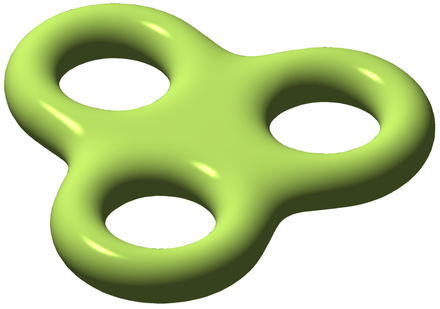
\includegraphics[scale = 1]{RiemannSurface}
**** Riemann Surface of genus 3, from Wikimedia ****

Of course this definition does not apply to curves over fields other than $\CC$, and doesn't relate the genus to the algebra of the curve. However, we can relate the topological genus of a curve directly to its topological Euler characteristic
$
\chi_{top}(C) = 2-2g.
$
By the Hopf index theorem, the topological Euler characteristic is the degree of the tangent sheaf, or equivalently, minus the degree of the cotangent sheaf $\omega_{C}$; that is, $\deg K_{C} = 2g-2$, and thus

$$
g(C) = \frac{\deg(K_C)}{2} + 1.
$$
(This formula serves to define the genus of a smooth projective curve over any field).

Other characterizations of the genus require more machinery to establish. We will give some here, and use  tools from the following section to prove equivalence.

\begin{enumerate}

\item\label{genus 1forms} $g(C)$ is the dimension of the vector space of regular 1-forms (that is, global sections of the
cotangent sheaf) on $C$.

\item The (Zariski) Euler characteristic of the structure sheaf of $C$ is $\chi(\cO_C) = h^0(\cO_C) - h^1(\cO_C)$. Since $h^0(\cO_C) = 1$, 
$$
g(C) = 1 - \chi(\cO_C).
$$

Recall that if $X\subset \PP^{r} = \PP(V)$ is any projective scheme, the \emph{homogeneous coordinate ring} of $X$
is the ring $S/I(X)$ where $S = \Sym V \cong \CC[x_{0}, \dots, x_{r}]$ and $I(V)\subset S$ is the ideal of homogeneous
forms that vanish on $X$.

\item\label{genus Hilbert} Suppose that $C \subset \PP^r = \PP(V)$ is a smooth curve of degree $d$  with homogeneous coordinate ring
$S_C$, then the function $d \mapsto \dim_\CC (S_C)_d$ is equal to a polynomial function $p_C(m)$ for large $d$. We have:
$$
p_C(m) =  dm - g + 1,
$$
so $g(C) = 1 - p_C(0)$. 
\end{enumerate}

\subsection{The Riemann-Roch Theorem}

To prove that these formulas for the genus are correct, we use \trr and Serre duality (sometimes called Kodaira-Serre duality, since Kodaira was responsible for the analytic version.)

\begin{theorem}[Riemann-Roch Theorem]\label{RR}
 If $C$ is a smooth, connected projective curve of genus $g$, and $D$ a divisor of degree $d$ on $C$ then
$$
h^0(D) = d - g + 1 + h^0(K_C - D).
$$
\end{theorem}

For example, if we take $D=0$, this tells us that $h^0(K) = g$, proving the characterization~(\ref{genus 1forms}) above. Also, since $h^0(D) = 0$ for any divisor $D$ of negative degree, the formula gives the dimension of $h^{0}(D)$ when $\deg D$ is large:

\begin{corollary}\label{nonspecial RR}
For any divisor of degree $d \geq 2g-1$, we have
$$
h^0(D) = d - g + 1.
$$
\end{corollary}

Using this, we can apply Proposition~\ref{very ample} to show that all high degree divisors come from embeddings:

\begin{corollary}\label{degree 2g+1 embedding}
Let $D$ be a divisor of degree $d$ on a smooth, connected projective curve of genus $g$. If $d \geq 2g$, the complete linear series $|D|$ is base point free; and if $d \geq 2g+1$ the associated morphism $\phi_D : C \to \PP^{d-g}$ is an embedding, so that
$D$ is the preimage of the intersection of $C$ with a hyperplane in $ \PP^{d-g}$.
\end{corollary}

Since the complement of a hyperplane in projective space is an affine space, we get an affine embedding result too:

\begin{corollary}
 If $C$ is any smooth, connected projective curve and $\emptyset \neq \Gamma \subset C$ a finite subset then $C \setminus \Gamma$ is affine.
\end{corollary}
\begin{proof}
Let $D$ be the divisor defined by $\Gamma$ By Corollary~\ref{degree 2g+1 embedding} a high multiple of $D$ is very ample,
and gives an embedding $\phi: C\to \PP^n$ such that the preimage of the intersection of $C$ with some hyperplane $H$
is a multiple of $D$. It follows that $C\setminus \Gamma$ is embedded in $\PP^n\setminus H$.
\end{proof}


We can  use \TRR in the simple case of Corollary~\ref{nonspecial RR} to determine the Hilbert polynomial of a projective curve. To do this, let $C \subset \PP^r$ be a smooth curve of degree $d$ and genus $g$, and consider the exact sequence of sheaves
$$
0 \rTo \cI_{C/\PP^r}(m) \rTo \cO_{\PP^r}(m) \rTo \cO_C(m) \rTo 0
$$
and the corresponding exact sequence
$$
 H^0(\cO_{\PP^r}(m)) \rTo^{\rho_m} H^0(\cO_C(m)) \rTo H^1(\cI_{C/\PP^r}(m)) \rTo 0.
$$

The \emph{Hilbert function} $h_C$ of $C$  is defined by
$$
h_C(m) = \dim_{\CC} (S_{C})_{m} = \rank(\rho_m).
$$
By Theorem~\ref{Serre vanishing} we have $H^1(\cI_{C/\PP^r}(m)) = 0$ for large $m$, so $h_{C}(m) = h^0(\cO_C(m))$, for large $m$, which, by \trr, equals $md-g+1$, again for large $m$. Thus, the Hilbert polynomial of $C \subset \PP^r$ is $p_C(m) = dm-g+1$, establishing the characterization~(\ref{genus Hilbert}).
 
The Riemann-Roch formula does \emph{not} give us a formula for the dimension $h^0(D)$ when $h^0(K_C - D)>0$; such divisors $D$ are called \emph{special divisors}, or \emph{special divisor classes}. The existence or non-existence of divisors $D$ with given $h^{0}(D)$ and $h^{1}(D)$ often serves to distinguish one curve from another, and will be an important part of our study.
 
 
\begin{fact}
 Classically, the dimension $h^0(K_C-D) = h^1(D)$ was called the \emph{superabundance} of $D$: the idea was that a divisor of degree $d$ had, at a minimum, $d-g+1$ sections and $h^1(D)$ represented the number of ``extra" sections. Even though the introduction of cohomology was still almost a century away, the ranks of cohomology groups $h^1$ had classical names, often involving the term superabundance---a premonition of the Riemann-Roch theorem in general.
\end{fact}
 
\begin{fact}
If $k$ is a field that is not algebraically closed there may be genus 0 curves that are not isomorphic to $\PP^1$. However, they must be``forms'' of $\PP^1$ in the sense that they become isomorphic to $\PP^1$ after extension of scalars to 
the algebraic closure $\overline k$ of $k$. The unique example with $k = \RR$ is the conic $x^2+y^2+z^2 = 0$. Indeed, any form of $\PP^1$ over any field $k$ can all be embedded in $\PP_{k}^2$ (by using the anti-canonical linear system.

The curve $\PP_k^1$ itself may be described as the scheme of left ideals of $k$-vector-space dimension 1 in the ring of
$2\times 2$ matrices over $k$ (such an ideal can be embedded in the matrix ring as a linear combination of the 2 columns in an appropriate sense). More generally, any scheme that is a form of $\PP^1$ over $k$
may be described as the scheme of 1-dimensional left ideals in a central simple ($=$ Azumaya) algebra over $k$---though as a set this scheme has no $k$-rational points unless the algebra is the algebra of $2\times 2$ matrices!
\end{fact}
\subsection{Serre duality}

In general, if $\cF$ and $\cG$ are coherent sheaves on a scheme $X$, we have for every $i$ and $j$ a cup product map
$$
H^i(\cF) \otimes H^j(\cG) \to H^{i+j}(\cF \otimes \cG).
$$

\begin{theorem}[Serre Duality]\label{sd} Let $C$ be a smooth connected projective curves with canonical divisor $K$. We have
 $$
h^1(K) = 1
$$
and the cup product map
$$
H^1(D) \otimes H^0(K-D) \to H^1(K)
$$
is a perfect pairing; that is, it induces a natural isomorphism
$$
H^1(D) = H^0(K-D)^*.
$$
\end{theorem}

\subsection{A partial proof}

Combining \TRR and Serre Duality we get:
\begin{corollary}
 If $C$ is a smooth, connected projective curve and $D$ is a divisor on $C$ then
\end{corollary}
$$
\chi(\sO_C(C)) := h^0(D) - h^1(D) = d-g+1
$$
or in other words, for any invertible sheaf $\cL$ of degree $d$ on $C$,
$$
\chi(\cL) = d-g+1
$$
which is pretty easy to prove. To see this, observe that for any invertible sheaf $\cL$ on $C$ and any point $p \in C$ we have an exact sequence of sheaves
$$
0 \to \cL(-p) \to \cL \to \cL_p \to 0.
$$
It follows that $\chi(\cL(-p)) = \chi(\cL) - 1$, so that Riemann-Roch for $\cL$ is equivalent to Riemann-Roch for $\cL(-p)$. Since any divisor can be obtained from 0 by adding and subtracting points, the Riemann-Roch formula for an arbitrary $\cL$ follows from the special case $\cL = \cO_C$.

\subsection{Clifford's theorem}

\begin{theorem}\label{Clifford}
Let $C$ be a curve of genus $g$ and $\cL$ a line bundle of degree $d \leq 2g-2$. Then
$$
r(\cL) \leq \frac{d}{2}.
$$
Moreover, if  equality holds then we must have either
\begin{enumerate}
\item $d=0$ and $\cL = \cO_C$;
\item $d = 2g-2$ and $\cL = K_C$; or
\item $C$ is hyperelliptic, and $|\cL|$ is a multiple of the $g^1_2$ on $C$.
\end{enumerate}
\end{theorem}

\begin{proof}
The proof of Clifford rests on a very basic construction and observation. 

To start, let $\cD = (\cL,V)$ and $\cE = (\cM, W)$ be two linear series on a curve $C$. By the \emph{sum} $\cD + \cE$ of $\cD$ and $\cE$, we will mean the pair 
$$
\cD + \cE = (\cL \otimes \cM, U) 
$$
where $U \subset H^0(\cL \otimes \cM)$ is the subspace generated by the image of $V \otimes W$, under the multiplication/cup product map $H^0(\cL) \otimes H^0(\cM) \to H^0(\cL \otimes \cM)$---in other words, it's the subspace of the complete linear series $|\cL\otimes \cM|$ spanned by divisors of the form $D+E$, with $D \in \cD$ and $E \in \cE$.

The observation is a simple one:
\begin{lemma}
If $\cD$ and $\cE$ are two nonempty linear series on a curve $C$, then
$$
\dim(\cD + \cE) \geq \dim \cD + \dim \cE.
$$
\end{lemma}
(To see this, we observe that to say $\dim \cD \geq m$ means exactly that we can find a divisor $D \in \cD$ containing any given $m$ points of $C$; since $\cD + \cE$ contains all pairwise sums $D + E$ with $D \in \cD$ and $E \in \cE$, we can certainly find a divisor $F \in cD + \cE$ containing any given $\dim \cD + \dim \cE$ points of $C$.)

Given this lemma, the proof of Clifford follows simply by applying it to the pair $|\cL|$ and $|K_C\otimes \cL^{-1}|$: by Riemann-Roch, we have
$$
r(K_C\otimes \cL^{-1}) = r(\cL) +g - d - 1
$$
and so we deduce that
$$
g = r(K_C) + 1 \geq r(\cL) + r(K_C\otimes \cL^{-1}) + 1 \geq 2r(\cL) +g - d;
$$
hence $r(\cL) \leq d/2$.

Our proof of the second half of Clifford rests on a basic fact about the geometry of hyperplane sections of a curve in projective space (Proposition~\ref{monodromy of hyperplane section}); we'll defer it until we've established that fact.
\end{proof}



\section{The canonical morphism}

Given the central role played by the canonical divisor class, it is natural to look at the geometry of the morphism $\phi_K : C \to \PP^{g-1}$ associated to the complete canonical series $|K|$.  By the Riemann-Roch theorem, 
$h^{0}(K) = g(C)$, so $|K|$ cannot define a non-constant morphism unless $g(C)\geq 2$, and cannot define an embedding unless $g(C)\geq 3$.

\begin{definition}
A curve $C$ of genus $g \geq 2$ is said to be \emph{hyperelliptic} if there exists a morphism $f: C \to \PP^1$ of degree 2. \end{definition}

%equivalently, if there exists a invertible sheaf $\cL$ on $C$ of degree 2 with $h^0(\cL) = 2$.

\begin{proposition}
The canonical morphism $\phi_K : C \to \PP^{g-1}$ is an embedding if and only if $C$ is not hyperelliptic.
\end{proposition}

\begin{proof}
By Corollary~\ref{degree 2g+1 embedding} we have to show that for any pair of points $p, q \in C$ we have
$$
h^0(K_C(-p-q)) = h^0(K_C)-2 = g-2.
$$
Applying \trr we see that this would fail if and only if $h^0(\cO_C(p+q)) \geq 2$ for some $p,q \in C$, and by Lemma~\ref{deg 2 morphism} $|p+q|$ would define a degree 2 morphism to $\PP^{1}$. 
\end{proof}

\begin{lemma}\label{deg 2 morphism}
Let $C$ be a smooth, projective curve of genus $g\geq 2$. Any invertible sheaf of degree 2 on $C$ defines a morphism to $\PP^{1}$. In particular, if $g(C) = 2$ then the canonical series $|K_{C}|$ defines a 2 to 1 morphism to $\PP^{1}$.
\end{lemma}

\begin{proof}
 If this happens,
we claim that $\cO_C(p+q)$ is basepoint free, so that $C$ is hyperelliptic. To finish the proof, by Corollary~\ref{degree 2g+1 embedding} it suffices to show that
 an invertible sheaf $\sL$ of degree 1 on $C$ must have $h^{0}(\sL)\leq 1$.
 
Suppose that $\sigma_{0}, \sigma_{1}$ were two linearly independent sections of $\sL$. Each $\sigma_{i}$ vanishes at a unique point $p_{i}$. If $p_{0}= p_{1}$ then a linear combination of $\sigma_{0}, \sigma_{1}$ would be a section vanishing to order $\geq 2$, which is impossible, so $\sL$ is basepoint free, and defines a degree 1 morphism $C\to \PP^{1}$. Such a morphism must be an isomorphism (because $\PP^{1}$ is normal), contradicting $g(C) \geq 2$.
\end{proof}

\fix{the following argument is only set-theoretic. Admit this or make it precise}
Note that if $C$ is hyperelliptic, the morphism $\phi_K$ factors through the degree 2 morphism $\pi : C \to \PP^1$: if $\{p,q\} \subset C$ is a fiber of this morphism, we have $h^0(\cO_C(p+q)) = 2$ and hence $\phi_K(p) = \phi_K(q)$. The image of the morphism $\phi_K$ is a nondegenerate curve of degree $g-1$ in $\PP^{g-1}$, which we will see is a \emph{rational normal curve}. This observation implies in particular that if $C$ is hyperelliptic of genus $g \geq 2$, then the invertible sheaf $\cL$ of degree 2 with $h^0(\cL) = 2$ is in fact unique.

Among curves with $g \geq 3$ the hyperelliptic curves are very special: in the family of all curves, as we'll see, they comprise a closed subvariety. Also, the behavior of linear series and morphisms on a hyperelliptic curve is very different from that of series on a general curve; when we discuss the geometry of curves of low genus in the Chapter~\ref{}, we will exclude  the hyperelliptic case, and deal with this case in a separate chapter.

For non-hyperelliptic curves, however, the geometry of the canonical morphism, and its image, the canonical curve, are the keys to understanding the curve. We'll see this in detail in many cases in the following chapter; for now, we mention one highly useful result along these lines.

\fix{add here: canonical series on plane curves cut by $|\cO_{\PP^2}(d-3)|$; consequence that no smooth plane curve can be hyperelliptic}

\fix{maybe move initial discussion of hyperelliptic curves from Ch. 6 to a section here}

\fix{maybe add to this chapter: differentials on plane curves $C$, possibly with nodes or more general singularities; adjoint conditions; algorithm for determining the complete linear system associated to a divisor $D$ on $C$}

\subsection{The geometric Riemann-Roch theorem}

Let's state this first in a relatively simple case: let $C$ be a nonhyperelliptic curve, embedded in $\PP^{g-1}$ by its canonical series and let $D = p_1+\dots + p_d$ be a divisor consisting of $d$ distinct points; let $\overline D$ be the span of the points $p_i \in C \subset \PP^{g-1}$. Since the hyperplanes in $\PP^{g-1}$ containing $\{p_1,\dots,p_d\}$ correspond (up to scalars) to sections of $K_C$ vanishing at all the points $p_i$, we see that
$$
h^0(K_C-D) = g - 1 - \dim \overline D.
$$
Plugging this into the Riemann-Roch formula, we arrive at the statement
$$
r(D) = d - 1 - \dim \overline D;
$$
or in other words, \emph{the dimension of the linear series $|D|$ in which the divisor $D$ moves is equal to the number of linear relations on the points $p_i$ on the canonical curve}. Thus, for example, if $D = p_1+p_2+p_3$, we see that $D$ moves in a pencil if and only if the points $p_i$ are collinear.

We can extend this statement to the case of arbitrary effective divisors $D$ (and even hyperelliptic curves) if we define our terms correctly. To do this, suppose $f : C \to \PP^d$ is any morphism, and $D \subset C$ any divisor. We define the \emph{span} of  $f(D)$ to be the intersection
$$
\overline{f(D)} = \bigcap_{H \mid f^{-1}(H)\supset D} H 
$$
of all hyperplanes in $\PP^d$ whose preimage in $C$ contains $D$. 

\begin{theorem}[Geometric Riemann-Roch Theorem]\label{geometric RR}
If $C$ is any curve of genus $g \geq 2$,  $\phi : C \to \PP^{g-1}$ its canonical morphism and $D \subset C$ any effective divisor of degree $d$, then
$$
r(D) = d - 1 - \dim \overline{\phi(D)}.
$$
\end{theorem}
 

\input footer.tex
%header and footer for separate chapter files

\ifx\whole\undefined
\documentclass[12pt, leqno]{book}
\usepackage{graphicx}
\input style-for-curves.sty
\usepackage{hyperref}
\usepackage{showkeys} %This shows the labels.
%\usepackage{SLAG,msribib,local}
%\usepackage{amsmath,amscd,amsthm,amssymb,amsxtra,latexsym,epsfig,epic,graphics}
%\usepackage[matrix,arrow,curve]{xy}
%\usepackage{graphicx}
%\usepackage{diagrams}
%
%%\usepackage{amsrefs}
%%%%%%%%%%%%%%%%%%%%%%%%%%%%%%%%%%%%%%%%%%
%%\textwidth16cm
%%\textheight20cm
%%\topmargin-2cm
%\oddsidemargin.8cm
%\evensidemargin1cm
%
%%%%%%Definitions
%\input preamble.tex
%\input style-for-curves.sty
%\def\TU{{\bf U}}
%\def\AA{{\mathbb A}}
%\def\BB{{\mathbb B}}
%\def\CC{{\mathbb C}}
%\def\QQ{{\mathbb Q}}
%\def\RR{{\mathbb R}}
%\def\facet{{\bf facet}}
%\def\image{{\rm image}}
%\def\cE{{\cal E}}
%\def\cF{{\cal F}}
%\def\cG{{\cal G}}
%\def\cH{{\cal H}}
%\def\cHom{{{\cal H}om}}
%\def\h{{\rm h}}
% \def\bs{{Boij-S\"oderberg{} }}
%
%\makeatletter
%\def\Ddots{\mathinner{\mkern1mu\raise\p@
%\vbox{\kern7\p@\hbox{.}}\mkern2mu
%\raise4\p@\hbox{.}\mkern2mu\raise7\p@\hbox{.}\mkern1mu}}
%\makeatother

%%
%\pagestyle{myheadings}

%\input style-for-curves.tex
%\documentclass{cambridge7A}
%\usepackage{hatcher_revised} 
%\usepackage{3264}
   
\errorcontextlines=1000
%\usepackage{makeidx}
\let\see\relax
\usepackage{makeidx}
\makeindex
% \index{word} in the doc; \index{variety!algebraic} gives variety, algebraic
% PUT a % after each \index{***}

\overfullrule=5pt
\catcode`\@\active
\def@{\mskip1.5mu} %produce a small space in math with an @

\title{Personalities of Curves}
\author{\copyright David Eisenbud and Joe Harris}
%%\includeonly{%
%0-intro,01-ChowRingDogma,02-FirstExamples,03-Grassmannians,04-GeneralGrassmannians
%,05-VectorBundlesAndChernClasses,06-LinesOnHypersurfaces,07-SingularElementsOfLinearSeries,
%08-ParameterSpaces,
%bib
%}

\date{\today}
%%\date{}
%\title{Curves}
%%{\normalsize ***Preliminary Version***}} 
%\author{David Eisenbud and Joe Harris }
%
%\begin{document}

\begin{document}
\maketitle

\pagenumbering{roman}
\setcounter{page}{5}
%\begin{5}
%\end{5}
\pagenumbering{arabic}
\tableofcontents
\fi


\chapter{Curves of genus 0 and 1}\label{genus 0 and 1 chapter}

In this chapter, we'll begin our project of describing curves in projective space with the simplest cases, that of curves of genus 0 and 1. Despite the relative simplicity of these curves, there are many interesting statements to make about the geometry of their embeddings in $\PP^r$, as well as many conjectures and open problems.

One reason for restricting our attention (for now!) to the cases $g=0$ and $1$ is that the divisor class theory is particularly simple in these cases. Specifically, on a curve of genus 0, there is a unique invertible sheaf of given degree $d$; and on a curve of genus 1 all invertible sheaves of given degree $d$ are congruent modulo the automorphism group of the curve. Thus, in regard to the geometry of the associated maps to projective space, all invertible sheaves of given degree $d$ behave in the same way. By contrast, on a curve $C$ of higher genus there are many different divisor classes of given degree, and to describe their various geometries we need to  introduce and describe the space $\Pic^d(C)$ parametrizing these invertible sheaves. We will do that in the following chapter, and then return in Chapter~\ref{genus 2 and 3 chapter} to the geometry of curves of genera 2 and 3 in projective space. 

Our knowledge of the geometry of curves becomes increasingly less complete as the genus increases, and 6, as we shall see, is a natural turning point; we will consider the case of curves of genus $, 5$ and $6$ in Chapter~\ref{genus 4, 5 and 6 chapter}


\section{Curves of genus 0} 


As we saw in more generality in Example~\ref{linear systems on Pr}, there is for each $d \in \ZZ$  a unique invertible sheaf $\cO_{\PP1} (d)$
of degree $d$ on $\PP^1$. To compute $H^0(\cO_{\PP1} (d))$ directly, let $D = z_1 +z_2 +\cdots+z_d$ be a divisor of degree d and suppose that the coordinates are chosen so that none of the $z_i$ are at infinity. The sections of $\cO_{\PP1} (D)$ are the rational functions with poles only at 
the $z_i$. In affine coordinates, identifying the $z_i$ with complex numbers, these can each be written
$$
\frac{g(z)}{(z-z_1)(z-z_2)\cdots(z-z_d)}
$$
with $\deg(g) \leq d$, the condition that infinity is not a pole. We see that these form a vector space of dimension $d+1$.

\fix{the following result is such a good exercise in the correspondence of linear systems and maps and divisors, maybe move it to Ch 2?}


By \trr, any invertible sheaf of degree $d$ on a curve of genus 0, like $\PP^1$, has at least $d+1$ sections. In fact (over $\CC$, or any algebraically
closed field), this characterizes $\PP^1$:

\begin{theorem}\label{characterization of P1}
Let $C$ be a reduced, irreducible projective curve and let $\cL$ be an invertible sheaf of degree $d$ on $C$. If $\h^0(\cL) \geq d+1$ then
$C \cong \PP^1$, so $\cL \cong \cO_{\PP^1}(d)$, and $\h^0(\cL) = d+1$. 
\end{theorem}

\begin{proof}
Let $p_1,\dots p_{d-1}$ be general points of $C$, and set $\cL':=\cL(-p_1-\cdots-p_{d-1})$. From the correspondence between divisors and
invertible sheaves, we see that the degree of $\cL'$ is $1$.
 Since $\cL$ is locally isomorphic to the sheaf of functions on $C$, the condition of vanishing at a point imposes at most 1 linear condition on 
the global sections of $\cL$, and thus $H^0(\cL') \geq 2$, so we may assume from the outset that $d =1$.

The linear system $(\cL, H^0(\cL))$ cannot have any base points, since
otherwise after subtracting one, we would get an invertible sheaf of degree $\leq 0$ with two independent global sections. Again by the correspondence
with divisors, neither of these sections could vanish at any point of $C$, so their ratio would be a non-constant function defined everywhere on $C$,
a contradiction.

Thus we see that the linear system $(\cL, H^0(\cL))$ defines a morphism $\phi: C\to \PP^1$ of degree 1 whose fibers---the divisors defined by
sections of $\cL$ are of degree 1. Thus if $p\in C$ is the preimage of $q\in \PP^1$, the induced map of local rings
$\phi^*:\cO_{\PP^1, q} \to \cO_{C, p}$ is a finite, birational map. Since $\cO_{\PP^1, q}$ is integrally closed, this is an isomorphism. Thus 
$\phi$ is an isomorphism, as required. 
 \end{proof}

Note that we used the algebraic closure of the ground field in choosing points on $C$.


\begin{corollary}
 Every smooth curve $C$ of genus 0 over an algebraically closed field is isomorphic to $\PP^1$.
\end{corollary}

\begin{proof}
 By \trr, any linear system $\cL$ of degree $d$ on $C$ has $h^0\cL \geq d+1$.
\end{proof}

Note that all the above depends fundamentally on the algebraic closure of the ground field: over a non-algebraically closed field, a curve $C$ of genus 0 need not have any points, or any line bundles of odd degree (since the canonical bundle $K_C$ has degree $-2$, there do necessarily exist line bundles of every even degree; thus an arbitrary curve of genus 0 is isomorphic to a conic plane curve). 
The classification of curves of genus 0 over non-algebraically closed fields is a subject that goes back to Gauss.

%\begin{fact}
%The left ideals of the ring of $2\times 2$ matrices 
%over any field can be indexed by the points of $\PP^1$: to the point $(\lambda, \mu)$ we associate the set of matrices 
%$$\biggl\{
%\begin{pmatrix}
% x_{1,1}&x_{1,2}\\
%  x_{2,1}&x_{2,2}
%\end{pmatrix} \mid \lambda  x_{1,1}+ \mu x_{1,2} = 0,\ \lambda  x_{2,1}+ \mu x_{2,2} = 0\biggr\};
%$$
%for example $(0,1)$ corresponds to the set of matrices with 0 in the second column.
%\def\bH{{\mathbb H}}
%The quaternion algebra 
%$$
%\bH := \RR<i,j,k>/(i^2 = j^2 = -1, ij=k = -ji)
%$$
% is a division ring, so it has no non-trivial left ideals, but
%we can still define the scheme of 2-dimensional left ideals to be the subscheme of the Grassmannian
%$G(2,\bH)$ consisting of 2-dimensional subspaces stable under multiplication by $i,j,k$. This subscheme, which can also be identified with the ``pointless'' conic $x^2+y^2+z^2 = 0$ in $\PP^2_\RR$ has no
%$\RR$-rational points, but $\CC\otimes_\RR \bH$ is the ring of $2\times 2$ matrices over $\CC$, so the set of $\CC$-points
%of the scheme of left ideals of $\bH$ may be identified with $\PP^1_\CC$. It turns out that every scheme over a field $k$ that
%becomes $\PP^1$ over the algebraic closure can be constructed as the scheme of left ideals of a 4-dimensional
%Azumaya (that is, central simple) algebra, in this case a (generalized) quaterion algebra, and as a smooth conic in $\PP^2_k$. There is also a cohomological
%description. See for example Serre ****\fix{I think its in Groupes Algebriques et Corps de Classes, but I'm not sure.}.
%\end{fact}


\section{Rational Normal Curves}

Recall from Example~\ref{Veronese definition} that the image of the $d$-th \emph{Veronese map}  $\phi_d: \PP^1 \to \PP(H^0((\cO_{\PP^1}(d)) \cong \PP^d$ is called the \emph{rational normal curve} of degree $d$. Rational normal curves are probably the most ubiquitous curves in projective space; they have many unique properties, and are extremal in many respects. We will accordingly take a few pages and list some of the special properties of rational normal curves.

\subsubsection{Rational normal curves have minimal degree}
The first is a characterization of rational normal curves as having smallest possible degree among irreducible, nondegenerate curves:

\begin{proposition}
If $C$ is a nondegenerate curve in $\PP^d$ then $\deg C \geq d$, with equality if and only if $C$ is a  rational normal curve.
\end{proposition}

\begin{proof}
 By the correspondence between morphisms and linear systems, the invertible sheaf $\cL$ corresponding to the morphism $C \hookrightarrow \PP^d$ has degree $d$ and
 $h^0(\cL) \geq d+1$. The conclusion follows from Theorem~\ref{characterization of P1}.
\end{proof}

We will see more generally that, if $X$ is a non-degenerate variety in $\PP^d$ of dimension $k$, then $\deg(X) \geq d-k+1$; and we will describe the varieties that achieve the minimum in Section~\ref{**}.

\subsubsection{Independence of points on a rational normal curve}

The points on a rational normal curve are ``as independent as possible:"

\begin{proposition}
If $C\subset \PP^d$ is a rational normal curve of degree $d$ and $\Gamma\subset C$ is a subscheme of length $\ell \leq d+1$, then
$\Gamma$ lies on no plane of dimension $<\ell$. In particular, any $m \leq d+1$ distinct points on a rational normal curve $C \subset \PP^d$ are linearly independent.
\end{proposition}

The rational normal curve is the unique curve with this property, as we shall see in Chapter~\ref{InflectionsChapter}. 

\begin{proof}
We can reduce to the case $\ell = d+1$ by adding points to $\Gamma$, so it suffices to do that case, which follows at once from Bezout's Theorem.
\end{proof}

In the case of distinct points it is easy to make a direct argument: In affine coordinates chosen so that none of the points are
at infinity we can identify the points $\lambda_1,\dots,\lambda_{d+1} \in C \cong \PP^1$ with complex numbers, and the statement (for $\ell = d+1$) is tantamount to the nonvanishing of the Vandermonde determinant
$$
\begin{vmatrix}
1 & \lambda_1 & \lambda_1^2 & \dots & \lambda_1^d \\
1 & \lambda_2 & \lambda_2^2 & \dots & \lambda_2^d \\
\vdots & & & & \vdots \\
1 & \lambda_{d+1} & \lambda_{d+1}^2 & \dots & \lambda_{d+1}^d \\
\end{vmatrix}.
$$

\subsubsection{Rational normal curves are projectively normal}


We say that a smooth curve $C \subset \PP^d$ is \emph{projectively normal} if the restriction map
$$
H^0(\cO_{\PP^d}(m)) \; \to \; H^0(\cO_{C}(m)) 
$$
is surjective for every $m$. We'll this property it in many settings, in particular the discussion of \emph{liaison} in Chapter~\ref{**}.
Since every monomial of degree $md$ on $\PP^1$ is a product of $m$ monomials of degree $d$, we see that the rational normal curve is projectively normal. 


\subsubsection{The equations defining a rational normal curve}
It is easy to write down equations that define a rational normal curve. Choosing a basis $s,t$ for the linear forms on $\PP^1$, we can write
$$
\phi_d : (s,t) \mapsto (s^d, s^{d-1}t,\dots t^d)
$$
from which we see that $C$ lies in the zero locus of the homogeneous quadratic polynomial $z_iz_j - z_kz_l$ for every $i+j=k+l$. As a convenient way to package these, we can realize these forms the $2\times 2$ minors of the matrix
$$
M \; = \; \begin{pmatrix}
z_0 & z_1 & \dots & z_{d-1} \\
z_1 & z_2 & \dots & z_d
\end{pmatrix}.
$$
Note that if we substitute $s^it^{(d-i)}$ for $z_i$ and identify $H^0(\cO_{\PP^1}(i)$ with $\CC[s,t]_i$, this becomes the multiplication table
$$
H^0(\cO_{\PP^1}(i)) \times H^0(\cO_{\PP^1}(d-i-1)) \to H^0(\cO_{\PP^1}(d));
$$
we shall see a general version of this in Chapter~\ref{ScrollsChapter}. 

In fact, the minors of this matrix generate the ideal of forms on $\PP^d$ vanishing on $C$. For this result see for example \cite[****]{E}. 
We can immediately prove two slightly weaker results:

First, $C$ is set-theoretically defined by the $2\times 2$ minors of $M$. Explicitly, suppose that $p = (z_0,\dots,z_d) \in \PP^d$ is any point, and all the polynomials $Q_{ijkl}$ above vanish at $p$. If $z_0 = 0$, then from the vanishing of 
$\det \begin{pmatrix}
z_0 & z_1  \\
z_1 & z_2 
\end{pmatrix}$ 
we see that $z_1 = 0$, and similarly we have $z_2 = \dots = z_{d-1}=0$; this the point $p = (0,\dots,0,1)$, which is a point on the rational normal curve. On the other hand, if $z_0 \neq 0$, set $\lambda = z_1/z_0$; we see in turn that $z_2/z_1 = \dots = z_d/z_{d-1} = \lambda$; thus $p = (1, \lambda, \dots,\lambda^d)$, again a point of the rational normal curve.

Second, the ${d\choose 2}$ distinct $2\times 2$ minors of $M$ are linearly independent, as one can see by first factoring out $x_0$ and $x_d$ and noting that the resulting minors generate the square of the maximal ideal in $\CC[x_1,\dots, x_{d-1}]$. Note that
the restriction map
$$
H^0(\cO_{\PP^d}(2)) \; \to \; H^0(\cO_{C}(2)) = H^0(\cO_{\PP^1}(2d))
$$
 is surjective  because every monomial of degree $2d$ on $\PP^1$ is a product of two monomials of degree $d$. Comparing dimensions, we see that the dimension of the kernel---that is, the space of quadratic polynomials on $\PP^d$ vanishing on $C$---has dimension
$$
\binom{d+2}{2} - (2d+1) \; = \; \binom{d}{2}.
$$


In fact, this gives us another characterization of rational normal curves as extremal: rational normal curves lie on more quadrichypersurfaces than any other irreducible, nondegenerate curve in $\PP^d$.

\begin{proposition}
If $C \subset \PP^d$ is any irreducible, nondegenerate curve, then
$$
h^0(\cI_{C/\PP^d}(2)) \leq  \binom{d}{2};
$$
and if equality holds then $C$ is a rational normal curve
\end{proposition}

\begin{proof}
Consider the restriction of the quadrics containing $C$ to a general hyperplane $H \cong \PP^{d-1} \subset \PP^d$, and let $\Gamma = H \cap C$. We have exact sequence:
$$
0 \to \cI_{C/\PP^d}(1) \to \cI_{C/\PP^d}(2) \to \cI_{\Gamma/\PP^{d-1}}(2) \to 0.
$$ 
Since $C$ is nondegenerate, $h^0(\cI_{C/\PP^d}(1)) = 0$, and since $\deg C \geq d$, the hyperplane section $\Gamma$ of $C$ must contain at least $d$ linearly independent points. Since linearly independent points impose independent conditions on quadrics, we have
$$
h^0(\cI_{\Gamma/\PP^{d-1}}(2)) \leq h^0(\cO_{\PP^{d-1}}(2)) - d,
$$
establishing the desired inequality.
\end{proof}

\begin{exercise}
Establish the analogous statement for hypersurfaces of any degree $d$; that is, no irreducible, nondegenerate curve in $\PP^r$ lies on more hypersurfaces of degree $d$ than the rational normal curve.
\end{exercise}

\begin{exercise}
Prove directly  the special case $r=3$: that the twisted cubic is the unique irreducible, nondegenerate space curve lying on three quadrics. (Hint: if $C \subset \PP^3$ is such a curve lying on three quadrics, what must be the intersection of two of the quadrics containing $C$?)
\end{exercise}

\subsubsection{Rational normal curves are projectively homogeneous}

Another important property of rational normal curves $C \subset \PP^d$ is that they are \emph{projectively homogeneous}: the subgroup $G$ of the automorphism group $PGL_{d+1}$ of automorphisms of $\PP^d$ that carries $C$ to itself acts transitively on $C$. More generally,
every $\PP^r$ is a homogeneous variety in the sense that $\Aut \PP^r$ acts transitively. If $\sigma$ is an automorphism then,
 because $\cO_{\PP^r}(d)$ is the unique
invertible sheaf of degree $d$ on $\PP^r$,  we have $\sigma^*\cO_{\PP^r}(d) = \cO_{\PP^r}(d)$ so $\sigma$ induces an automorphism $\phi$ on $H^0(\cO_{\PP^r}(d))$, and an automorphism $\overline \phi$ on the ambient space $\PP H^0(\cO_{\PP^r}(d))$ of the target of the $d$-th Veronese map. If $\alpha$
is a rational function with divisor $D$, then $\phi(\alpha) = \alpha\circ \sigma$ has divisor $\sigma^{-1}(D)$, so $\overline\phi^{-1}$ induces $\sigma$ on $\PP^r$. 

The rational normal curve $C \subset \PP^r$ can also be characterized among irreducible, nondegenerate curves as the unique projectively homogeneous curve in $\PP^r$, as we shall see in Chapter~\ref{InflectionsChapter}.

\begin{exercise}
Let $\PP^1 \hookrightarrow C \subset \PP^3$ be a twisted cubic. Show that the normal bundle $\cN_{C/\PP^3}$ (defined to be the quotient of the restriction $T_{\PP^3}|_C$ to $C$ of the tangent bundle  of $\PP^3$  by the tangent bundle $T_C$) is 
$$
\cN_{C/\PP^3} \cong \cO_{\PP^1}(5) \oplus  \cO_{\PP^1}(5)
$$
\end{exercise}

\begin{exercise}
Let $\PP^1 \hookrightarrow C \subset \PP^d$ be a rational normal curve. Show that the normal bundle $\cN_{C/\PP^d}$  is 
$$
\cN_{C/\PP^d} \cong \bigoplus_{i=1}^{d-1} \cO_{\PP^1}(d+2).
$$
\end{exercise}

\begin{exercise}
In the situation of the preceding problem, the set  of direct summands of $\cN_{C/\PP^d} $ is a projective space $\PP^{d-2}$. How does the  group of automorphisms of $\PP^d$ carrying $C$ to itself act on this $\PP^{d-2}$?

\end{exercise}

\subsection{Other rational curves}

What about other rational curves in projective space? There are many other embeddings of $\PP^1$ in $\PP^r$ other than the rational normal curve, and we'll talk now about some of these.

The first thing to say is that, since any linear series $\cD$ of degree $d$ on $\PP^1$ is a subseries of the complete series $|\cO_{\PP^1}(d)|$, we see that \emph{any rational curve $C \subset \PP^r$ of degree $d$ is a projection of a rational normal curve in $\PP^d$}. Slightly more generally, any map $\phi : \PP^1 \to \PP^r$ of degree $d$ is given as
$$
z \; \mapsto \; (f_0(z), \dots, f_r(z))
$$
for some $(r+1)$-tuple of polynomials $f_\alpha$ of degree $d$ on $\PP^1$, which is to say it is the composition of the embedding $\phi_d : \PP^1 \to \PP^d$ of $\PP^1$ as a rational normal curve with a linear projection $\pi : \PP^d \to \PP^r$. 

Given how easy it is to describe rational curves in projective space in this way, it is in some ways surprising how many open questions there are about such curves. We'll talk more about some of these questions in the following section; for now, we will try to give a sense of what we can say about such curves by considering one of the first and simplest cases: smooth rational curves of degree $4$ in $\PP^3$.

So: let $C \subset \PP^3$ be a smooth, nondegenerate curve of degree 4 and genus 0 in $\PP^3$. To describe the geometry of $C$, the first thing to determine is what surfaces it lies on---that is, what degree polynomials on $\PP^3$ vanish on $C$. 
\fix{what's proven is that $C$ lies on a smooth quadric and the ideal needs at least 3 additional 3-ic generators. State in advance, and maybe do better.}
To start with, we can ask: does $C$ lie on a quadric surface? To answer this, we consider again the restriction map
$$
H^0(\cO_{\PP^3}(2)) \; \to \; H^0(\cO_{C}(2)) = H^0(\cO_{\PP^1}(8)).
$$
Here the vector space on the left---homogeneous quadratic polynomials on $\PP^3$---has dimension 10, while the one on the right, either by Riemann-Roch or by direct examination, has dimension 9. We conclude that \emph{the curve $C$ must lie on at least one quadric surface $Q \subset \PP^3$}.

Since $C$ is irreducible and nondegenerate, it can't lie on a union of planes, so the quadric $Q$ must either be smooth or a cone over a conic curve. We'll see in a moment that the latter case can't occur, so let's assume for now that $Q$ is smooth. 

The natural follow-up question is, what is the class of $C$ in the Picard group of $Q$? We know that $Q \cong \PP^1 \times \PP^1$, with the fibers of the two projections appearing as lines of the two rulings of $Q$. Lines $L$ and $M$ of the two rulings generate the Picard group \cite[***]{H}, so that we must have $C \sim aL + bM$ for some $a, b$ (in other words, in terms of the isomorphism $Q \cong \PP^1 \times \PP^1$, $C$ is the zero locus of a bihomogeneous polynomial of bidegree $(a,b)$), and we ask what $a$ and $b$ are. The choices are limited: since $C$ is a quartic curve, we must have $a+b = 4$. Adjunction \cite[***]{H} tells us which must be the case: the genus formula for curves on $Q$ tells us that the genus of a smooth curve of class $(a,b)$ on $Q$ has genus $(a-1)(b-1)$, whence the class of our curve $C$ must be $(1,3)$ (for a suitable ordering of the two rulings).

It follows in particular that \emph{$Q$ is the unique quadric containing $C$}. One way to see this is that since $C$ has class $(1,3)$ it meets the lines of the first ruling three times; if $Q'$ is any quadric containing $C$, then, it must contain all these lines and hence must equal $Q$. Equivalently, we may consider the exact sequence
$$
0 \to \cI_{C/Q}(2) \to \cO_Q(2)  \to \cO_C(2) \to 0.
$$
If $C$ has class $L+3M$, we have $\cI_{C/Q}(2) = \cO_{Q}(L-M)$. Since this bundle has negative degree on every line of the first ruling, it has no sections; hence the restriction map $H^0(\cO_Q(2))  \to H^0(\cO_C(2))$ is injective and so there are no  quadrics in $\PP^3$ containing $C$ other than $Q$.

We can also describe the rest of the ideal of $C$ similarly. For example, to find the cubic polynomials vanishing on $C$ we consider the restriction map
$$
H^0(\cO_{\PP^3}(3)) \; \to \; H^0(\cO_{C}(3)) = H^0(\cO_{\PP^1}(12)).
$$
The dimensions of these two vector spaces being 20 and 13 respectively, we see that $C$ must lie on at least 7 cubics; four of these are simply products of $Q$ with linear forms, and so we see that $C$ must lie on at least three cubics modulo those containing $Q$. Indeed, these are easy to spot: if $L$ and $L'$ are any two lines of the first ruling, the divisor $C + L + L'$ has class $(3,3)$ on $Q$ and hence is the intersection of $Q$ with a cubic surface. As $L+L'$ varies in a two-dimensional linear series, we get three cubics containing $C$ modulo those containing $Q$. Conversely, any cubic containing $C$ (but not containing $Q$) will intersect $Q$ in the union of $C$ with a curve of type $(2,0)$ on $Q$, which is to say the sum of two lines of the first ruling, so these are all the cubics containing $C$.

\fix{at least state that these are the generators. And state the set-theoretic
intersection problem.}

Finally, we have to show that the quadric containing the curve $C$ cannot be a cone over a conic plane curve. The key question here is whether or not $C$ contains the vertex $p$ of the cone: if not, the same adjunction-based calculation shows that $C$ must have genus 1; while a parity argument (how many times does $C$ meet a line of the ruling of $Q$?) shows that if a curve $C \subset Q$ of even degree contains $p$ it must be singular there.\fix{this is pretty fast, compared to the level in the rest of the Ch. let's fill it in.}


\begin{exercise}
Find all possible Hilbert functions of smooth rational quintic  curves $C \subset \PP^3$. (There are only two, depending on whether or not $C$ lies on a quadric, so this isn't so bad.)
\end{exercise}

\begin{exercise}
Every $g^3_4$ on $\PP^1$ is uniquely expressible as a sum of the $g_1^1$ and a $g^1_3$
\end{exercise}

\begin{exercise}
There is a 1-parameter family of rational quartic curves in $\PP^3$ up to projective equivalence. (Finding the invariants is a nice problem, which we should talk about. This is the cross-ratio of the roots of the quartic in 2 variables corresponding to the projection center.)
\end{exercise}

\subsection{Further problems (open and otherwise) concerning rational curves in projective space}

To begin with, we should remark that this one example of a non-linearly normal rational curve in projective space is misleading in that we can give such a complete description. For general $d$ and $r$, we have no idea what may be the Hilbert function of a rational curve of degree $d$ in $\PP^r$. Indeed, even in the limited case of $r=3$, our knowledge gives out around $d=9$.

We can, however, say some things about a \emph{general} rational curve $C \subset \PP^r$ of given degree $d$. To make sense of this, let $C_0 \subset \PP^d$ be a rational normal curve of degree $d$. As we've said, any rational curve of degree $d$ in $\PP^r$ is the projection $\pi_\Lambda(C_0)$ of $C_0$ from a $(d-r-1)$-plane $\Lambda \subset \PP^d$. If we let $\GG = \GG(d-r-1, d)$ be the Grassmannian of $(d-r-1)$-planes in $\PP^d$, and we let $U \subset \GG$ be the open subset of planes disjoint from the secant variety of $C_0$, we have a family of rational curves in $\PP^r$ parametrized by $U$ and including every smooth rational curve $C \subset \PP^r$ of degree $d$. Thus in particular we can talk about a \emph{general rational curve} of degree $d$ and genus $g$ in $\PP^r$, and ask about its geometry.

This is, in fact, still largely uncharted waters. Consider, for example, one of the most basic questions we might ask: what is the Hilbert function of a general rational curve $C \subset \PP^r$ of degree $d$? As in the example, this is tantamount to looking at the restriction map
$$
\rho_m : H^0(\cO_{\PP^r}(m) \to H^0(\cO_C(m)) = H^0(\cO_{\PP^1}(md)).
$$
Equivalently, we're asking: if $V$ is a general  $(r+1)$-dimensional vector space of homogeneous polynomials of degree $d$, what is the dimension of the space of polynomials spanned by $m$-fold products of polynomials in $V$? We might naively guess that the answer is, ``as large as possible," meaning that the rank of $\rho_m$ is $\binom{m+r}{r}$ when that number is less than $md+1$, and equal to $md+1$ when it is greater---in other words, the map $\rho_m$ is either injective or surjective for each $m$.

This, it turns out, is true, but it is only relatively recently known: the case $g=0$, as here, was done by Ballico in **** (??), and the analogous statement for curves of arbitrary genus, which we will describe in Chapter~\ref{Brill-Noether}, was proved in 2019 by Eric Larson.

\subsubsection{The secant plane conjecture}

Another question we may ask about a curve in projective space is what secant planes it has. To frame the question, let's start with some language: given a smooth curve $C \subset \PP^r$, we say that an $e$-secant $s$-plane to $C$ is an $s$-plane $\Lambda \cong \PP^s \subset \PP^r$ such that the intersection $\Lambda \cap C$ has degree $\geq e$; if we exclude degenerate cases (for example, where $\Lambda \cap C$ fails to span $\Lambda$), this is the same as saying we have a divisor $D \subset C$ of degree $e$ whose span is contained in an $s$-plane.

Do we expect a curve $C \subset \PP^r$ to have any $e$-secant $s$-planes? The set of $s$-planes in $\PP^r$ is parametrized by the Grassmannian $\GG = \GG(s,r)$, which had dimension $(s+1)(r-s)$. Inside $\GG$, the locus of planes that meet $C$ has codimension $r-s-1$ (the locus of planes containing a given point of $C$ has codimension $r-s$); so our naive expectation might be that the locus of $e$-secant $s$-planes would have codimension $e(r-s-1)$ in $\GG$. Thus we would expect a curve $C \subset \PP^r$ to have $e$-secant $s$-planes when 
$$
e \; \leq \; (s+1)\frac{r-s}{r-s-1}.
$$
Is this true of a general rational curve? For most $e$, $r$ and $s$, we don't know!

\section{Curves of genus 1}

%Wonderful subject; refer to somewhere else. Double cover of $\PP^1$, leading to $y^2 - f(x)$. Plane cubic, quartic in $\PP^3$. Cheerful fact:  elliptic quintic is Pfaffian. Cheerful fact: any $g^5_6$ is the product of two $g^2_3$s. Get a $3\times 3$ matrix of linear forms. The image of the matrix and its transpose are $g^2_3$'s. Prove this by going to the Segre embedding $\PP^2\times \PP^2 \subset\PP^8$.

We cannot begin to describe everything that has been said or done with curves of genus 1, or \emph{elliptic curves}\footnote{Technically, an elliptic curve is a smooth curve of genus 1 with a distinguished point, called the \emph{origin}.}. They appeared, in the second half of the 19th century, as key objects in the developing subjects of geometry, number theory and complex analysis, and the literature is correspondingly rich. Though all curves of genus 0 are isomorphic to $\PP^1$ and on a given curve of genus 0 all divisors of a given degree are linearly equivalent, neither of the analogous statements holds true for curves of genus 1. The ways in which 19th century geometers dealt with this fact has shaped much of algebraic geometry.

Specifically, classical geometers observed that there was a one-parameter family of curves of genus 1 up to isomorphism, and that on a given curve of genus 1 there was a one-dimensional family of divisors up to linear equivalence. These were perhaps the earliest examples of \emph{moduli spaces}, and they were ultimately generalized to the moduli space $M_g$ of curves of genus $g$, and the Picard variety $\Pic^d(C)$ parametrizing divisors of degree $d$ on a given curve $C$ up to linear equivalence.

 Here we will focus on the geometric side, and try to describe maps of genus 1 curves to projective space. As a sort of through-line for our discussion, we will try to indicate in each case how the given projective model of a curve $E$ of genus 1 gives rise to the expectation that there is a one-parameter family of curves of genus 1 up to isomorphism. For any $d$, the automorphism group of $E$ acts transitively on the invertible sheaves of degree $d$ on $E$. In other words, if $\phi, \phi' : E \to \PP^r$ are two maps given by complete linear series $|L|$ and $|L'|$ of degree $d$ on $E$, then there exists  automorphisms $\alpha : \PP^r \to \PP^r$ and $\beta : E \to E$ such that $\phi' \circ \beta= \alpha \circ \phi$. In particular, if $\phi$ and $\phi'$ are embeddings---as will be the case when $d \geq 3$---then their images are projectively equivalent. As for the business of parametrizing invertible sheaves on a given curve $C$, we will take that up in the next chapter, and see it applied in the case of curves of genus $g \geq 2$ in Chapter~\ref{genus 2 and 3 chapter}.

\subsection{Double covers of $\PP^1$}

Let $E$ be a smooth projective curve of genus 1. If $L$ is any invertible sheaf of degree 1 on $E$, \trr says that $h^0(L) = 1$, so if we're looking for nonconstant maps to projective space we have to go to degree 2 and higher.

To start with, suppose $L$ is an invertible sheaf of degree 2 on $E$. By \trr, $h^0(L) = 2$ and the linear series $|L|$ is base point free, so we get a map $\phi : E \to \PP^1$ of degree 2. By \trh, the map $\phi$ will have 4 branch points; by the remark above, these four points are determined, up to automorphisms of $\PP^1$ by the curve $E$, and are independent of the choice of $L$.
After composing with an automorphism of $\PP^1$ we can take these four points to be $0, 1, \infty$ and $\lambda$ for some $\lambda \neq 0, 1 \in \CC$. Since there is a unique double cover of $\PP^1$ with given branch divisor (see~\ref{**}) it follows that $E \cong E_\lambda$, where $E_\lambda$ is the curve given by the affine equation
$$
y^2 = x(x-1)(x-\lambda).
$$

When are two curves $E_\lambda$ and $E_{\lambda'}$ isomorphic? By what we've said, this will be the case if and only if there is an automorphism of $\PP^1$ carrying the points $\{0,1,\infty,\lambda\}$ to $\{0,1,\infty,\lambda'\}$, in any order. This will be the case if and only if $\lambda$ and $\lambda'$ belong to the same orbit under the action of the group $G \cong S_3 \subset PGL(3)$ of automorphisms of $\PP^1$ permuting the three points $0, 1$ and $\infty$. Direct computation shows that the orbit of $\lambda$ is
$$
\lambda' \in \{\lambda, \; 1-\lambda, \; \frac{1}{\lambda},\;  \frac{1}{1-\lambda}, \; \frac{\lambda - 1}{\lambda}, \; \frac{\lambda}{\lambda - 1} \}.
$$
Now, the quotient of $\PP^1$ by the action of $G$ is again isomorphic to $\PP^1$ by Luroth's theorem, which means that the field of rational functions on $\PP^1$ invariant under $G$ is again a purely transcendental extension $K(j)$; explicitly, we can take
$$
j \; = \; 256\cdot \frac{\lambda^2 - \lambda + 1}{\lambda^2(\lambda - 1)^2}.
$$
(the factor of 256 is there for arithmetic reasons). In any case, we see explicitly that there is a unique smooth projective curve of genus 1 for each value of $j$; in particular, the family of all such curves is parametrized by a curve.

\subsection{Plane cubics}

Moving from degree 2 to degree 3, let $L$ be an invertible sheaf of degree 3 on $E$. We see from Corollary~\ref{degree 2g+1 embedding} that the sections of $L$ give an embedding of $E$ as a smooth plane cubic curve; conversely, the genus formula tells us that a smooth plane cubic curve indeed has genus 1. 

We won't delve into the geometry of plane cubics, except to point out that once more we can use this representation to argue that the isomorphism classes of elliptic curves form a 1-dimensional family. To see this, observe that the space of homogeneous polynomials of degree 3 in three variables is 10-dimensional, and the space of plane cubic curves is correspondingly parametrized by  $\PP^9$; the locus of smooth curves is a Zariski open subset of this $\PP^9$. On the other hand, by what we've said, two plane cubics are isomorphic iff they are congruent under the group $PGL_3$ of automorphisms of $\PP^2$. Since the group $PGL_3$ has dimension 8, we would expect that the family of such curves up to isomorphism has dimension 1.

\subsection{Quartics in $\PP^3$} 

Again, let $E$ be a smooth projective curve of genus 1, and consider now the embedding of $E$ into $\PP^3$ given by the sections of an invertible sheaf $L$ of degree 4. The first question we might ask is what polynomial equations in $\PP^3$ cut out the image, and as before we will do this by looking at the restriction map
$$
\rho_2 \;  : \; H^0(\cO_{\PP^3}(2)) \; \to \; H^0(\cO_{E}(2)) = H^0(L^2).
$$
The space on the right---the space of homogeneous polynomials of degree 2 in four variables---has dimension 10, while by Riemann-Roch the space $H^0(L^2)$ has dimension 8. It follows that $E$ lies on at least two linearly independent quadrics $Q$ and $Q'$. Since $E$ does not lie in any plane, neither $Q$ nor $Q'$ can be reducible; thus by \bt we see that
$$
E = Q \cap Q'
$$
is the complete intersection of two quadrics in $\PP^3$. Moreover, we also see from the Lasker-Noether ``AF+BG" theorem that the kernel of $\rho_2$ is exactly the span of $Q$ and $Q'$. Thus $E$ determines a point in the Grassmannian $G(2, H^0(\cO_{\PP^3}(2))) = G(2, 10)$ of pencils of quadrics; and by Bertini's Theorem, a Zariski open subset of that Grassmannian correspond to smooth quartic curves of genus 1. We can use this to once more calculate the dimension of the family of curves of genus 1: the Grassmannian $G(2,10)$ has dimension 16, while the group $PGL_4$ of automorphisms of $\PP^3$ has dimension 15, so we may conclude that the family of curves of genus 1 up to isomorphism has dimension 1.


\subsubsection{Projective normality II}
\fix{maybe this should be part of the homological algebra development much later}
Observe that last two cases (cubic and quartic genus 1 curves) are projectively normal; extend this to arbitrary smooth complete intersections.

Exercise: $C \subset Q \subset \PP^3$ of class $(a,b)$ is projectively normal iff $|a-b| \leq 1$.


\input footer.tex



\input header.tex

\chapter{Jacobians}\label{new Jacobians chapter}


An essential construction in studying a curve $C$ is the association to a divisor  of an invertible sheaf---in other words, the map
$$
\big\{ \text{effective divisors of degree $d$ on C}\big\} \rTo^\mu \big\{ \text{invertible sheaves of degree $d$ on C} \big\}.
$$
sending $D$ to $\cO_C(D)$.

A priori, this is a map of sets. But it is a fundamental fact that each set may  be given the structure of an algebraic variety in a natural way, so that the map between them is regular. The geometry of this map governs the geometry of the curve in many ways.
In this chapter we will describe the source and target of $\mu$, and give references to proofs of their properties. 

We start with the effective divisors. Since $C$ is smooth, an effective divisor of degree $d$ on $C$ is the same thing as a subscheme $D \subset C$ of dimension 0 and degree $d$, and thus
the family $C_d$ of effective divisors of degree $d$ on $C$ is a Hilbert scheme; see~\ref{hilbert scheme section}. This Hilbert scheme may be identified with
the $d$-th \emph{symmetric power} $C^(d)$  of $C$, described in Section~\ref{symmetric section}. 

The parametrization of the set of invertible sheaves on $C$ of a given degree $d$ by the variety $\Pic_d(C)$ requires different techniques. We will define it by a universal property in the category of schemes, and exhibit its construction as an analytic variety, actually a complex torus $\Jac(C)$, whose group structure reflects the tensor product of
sheaves in $\Pic_0(C)$.
Historically, the algebraic construction was a major milestone first reached in the work of Andre Weil in the middle of
the 20th century, and was the reshaped by Grothendieck and his school. The interested reader will find a beautiful, detailed account both of the history and the 
modern theory of the scheme of divisors and the Picard scheme in the exposition~\cite{Kleiman-PicardScheme}. We will give
more specific references to this text as we go, and the reader will find extensive references to the original literature there.

As an application of the mere existence of the spaces $C_d$ and $\Pic_d$, we show in Theorem~\ref{g+3 theorem} that a general divisor of degree $g+3$ on any curve of genus $g$ gives rise to an embedding in $\PP^3$ as a curve of degree $g+3$. Similar techniques, in Section~\ref{g+2 section} show that a general divisor of degree $g+2$ on any curve gives a birational morphism to a plane curve of degree $g+2$. Moreover, if the curve is not hyperelliptic then its image in $\PP^2$ has  only nodes
as singularities, while in the hyperelliptic case its only singularity is one ordinary $g$-fold point. 

\section{Symmetric products and the universal divisor}\label{symmetric section}

Let $C$ be a smooth curve. The space of effective divisors on $C$ can be characterized by a universal property. 

\begin{definition}
Let $B$ be any scheme. A \emph{family} of effective divisors of degree $d$ on $C$, parametrized by the scheme $B$, is a Cartier divisor $X\subset B\times C$ whose intersection with fibers $\{b\} \times C \cong C$ over points of $B$ are divisors of degree $d$ on $C$.
\end{definition}

Given this, we have a contravariant functor 
$$
F : (schemes) \to (sets),
$$
defined by taking a scheme $B$ to the set of families of divisors of degree $d$ over $B$; if $\pi : B' \to B$ is any morphism, the induced map $F(B) \to F(B')$ is defined by taking a family $\cD \subset B \times C$ to the preimage of $\cD$ under the map $\pi \times Id : B' \times C \to B \times C$. We say that a scheme $C_d$ is a fine moduli space for divisors of degree $d$ on $C$ if we have an isomorphism of functors
$$
F \cong \Hom_{\rm{Schemes}}( -, C_d).
$$
By Yoneda's Lemma, this is equivalent to the existence of a \emph{universal family} $\cD \subset C_d \times C$, with the property that for any family $X \subset B \times C$ of divisors on $C$ over any scheme $B$, there is a unique map $\phi : B \to C_d$ such that $X = (\phi \times id_{C})^{-1}(\cD)$.

From the universal property it is clear that a fine moduli space for divisors of degree $d$ on $C$ is unique if it exists. Indeed, it does exist, and we'll sketch the construction, using symmetric products. This construction relies on the existence of quotients of schemes by finite groups, and we'll pause here to discuss such quotients.

\subsection{Finite group quotients}

If $G$ is a finite group acting by automorphisms on an affine scheme $X:=\Spec A$ then $X/G$ is by definition $\Spec(A^G)$, the spectrum of the ring $A^G$ of invariant elements of $A$. The following result shows that this definition reflects the desired
geometry: 

\begin{theorem}\label{finite invariant theory}
 The map $\pi: X\to X/G$ induced by the inclusion of rings is finite. If $X$ is a normal variety, then the fibers of $\pi$  are the orbits of $G$.
\end{theorem}
For a proof, see for example \cite[Proposition 13.10]{Eisenbud1995}).  

Since the map $X\to X/G$ is finite, we have $\dim X/G = \dim X$. 

The construction commutes with the passage to $G$-invariant open affine sets, and thus passes to more general schemes---and in particular to projective schemes (Exercise~\ref{quotient of projective})---as well.

When the group $G$ is infinite, the situation becomes much more complex---see Chapter~\ref{ModuliChapter} for some  idea of what can and cannot be done.

For example, if $X$ is any scheme or any quasi-projective variety $X$ we define the \emph{$d$-th symmetric power $X^{(d)}$ of $X$} to be the quotient of the Cartesian product $X^d$ of $d$ copies of $X$ by the action of the group of permutations of the factors. 

%Since an effective divisor of degree $d$ on a curve $C$ is an unordered $d$-tuple of points on $C$, with repetitions allowed, it corresponds to a point in the \emph{$d$th symmetric power} $C^{(d)}$. For this reason we will write the points of $\Cd$ as $d$-tuples.

If $X=\AA^{1}$ then $X^{d} = \AA^{d} = \Spec \CC[x_{1}, \dots, x_{d}]$. The ring of invariants of the symmetric group acting on
$\CC[x_{1}, \dots, x_{d}]$ by permuting the variables is generated by the $d$ elementary symmetric functions, which generate a polynomial subring, and $X^{(d)}$ is isomorphic to $\AA^{d}$. Since the symmetric functions of the roots of a polynomial in one variable are the coefficients of
that polynomial, we may identify $X^{(d)}$ with the affine space of monic polynomials of degree $d$ in $\CC[z]$. (\cite[Exercises 1.6, 13.2-13.4]{Eisenbud1995})

Next consider $X = \PP^1$ and the product $(\PP^1)^d$. Taking the homogeneous coordinates of the
$i$-th copy of $\PP^1$ to be $(s_i,t_i)$, the $d+1 $multilinear symmetric functions of degree $d$,
$$
t_1t_2\cdots t_d,\ s_1t_2\cdots t_d,\ \dots,\ s_1\cdots s_d
$$
are the coefficients of the polynomial
$$
(s_1\lambda + t_1\mu)(s_2\lambda + t_2\mu)\cdots(s_d\lambda + t_d\mu)
$$
defining a general subcheme of $\PP^1$ of degree $d$ and  define
an isomorphism $(\PP^1)^{(d)} \to \PP^d$.
Again, we may think of this map as taking a $d$-tuple of points to the unique-up-to-scalars
homogeneous form of degree $d$ vanishing on it.

We shall see that when $C$ is a smooth curve of higher genus, the global geometry of $C^{(d)}$ is quite nontrivial, but at least
the local geometry is simple:

\begin{proposition}
If $C$ is a smooth curve then each symmetric power $C^{(d)}$ is smooth.
\end{proposition}

\begin{proof}
 The general case follows from the case of $\AA^{1}$ because locally analytically the action of the symmetric group on $C^d$ is the same as for $\AA^1$: If  $\overline p \in X^{(d)}$, then it suffices to
 show that the quotient of an invariant formal neighborhood of the preimage $p_1,\dots, p_s$ of
 $\overline p$ is smooth. After completing the local rings, we get an action of the symmetric group
 $G$ on the product of the completions of $X$ at the $p_i$, and this depends only on the orbit
 structure of $G$ acting on $\{p_1,\dots, p_s\}$. Thus it would be the same for some orbit of
 points on $\AA^1$.
 \end{proof}

By contrast, if $\dim X \geq 2$ then the symmetric powers $X^{(d)}$ are singular for all $d \geq 2$.
See Exercise~\ref{sym2A2} for the case of $(\AA^2)^{(2)}$ and Exercise~\ref{free actions} for a well-behaved case.

It is clear from Theorem~\ref{finite invariant theory} that the points of $C^{(d)}$ are in one-to-one correspondence with the effective divisors of
degree $d$ on $C$, but much more is true:

\begin{theorem}
 If $C$ is a smooth projective curve, then the $d$th symmetric power $C^{(d)}$ of $C$ is the fine moduli space $C_d$ for effective divisors of degree $d$ on $C$.
\end{theorem}
For a proof in the analytic category, see \cite[]{ACGH}; for the algebraic fact, see \cite[Remark 9.3.9]{Kleiman-PicardScheme}.
Henceforward we will write $C_d$ in place of $C^(d)$ for this space.


%Finally we come to the definition of the universal family:
%
%\begin{fact}
% The universal family of degree $d$ divisors on $C$ is the incidence correspondence $\sD\rTo^\alpha \Cd$ where
% $\sD \subset C \times \Cd$ is the incidence correspondence 
%$$
%\sD := \{(x,(x_1,\dots x_d)) \mid x = x_i\hbox{ for some }i\}.
%$$
%and thus the Hilbert scheme of degree $d$ subschemes of $C$ is $\Cd$.
%
%If $X \to C\times B$ is a family of divisors of degree $d$ on $C$ then we may define a set-theoretic map $\phi: B\to \Cd$ by sending $b\in B$ to the
%unordered $d$-tuple of points of the divisor that is the fiber over $b$. This together with the composition $X \to C \rTo^1 C$
%gives us the diagram in the Theorem, and it can be shown that the map $\phi$ is a map of schemes.
%\end{fact}

%\fix{seems a pity not to prove this -- we prove so little in this Chapter Kleiman's reference are to Deligne and the book by Bosch et al on Neron-Severi.}

\section{The Picard varieties}

As with $C_d$, we may define $\Pic_d(C)$ by a universal property. We start by saying what we mean by a family of invertible sheaves on a smooth curve $C$:

\begin{definition}
 For any scheme $B$, a \emph{family of invertible sheaves on $C$ over $B$} is an equivalence class of invertible sheaves $\sL$ on $B\times C$, where two such
 families $\sL$ and $\sL'$are equivalent if they differ by an invertible sheaf pulled back from $B$, that is, if
 $$
 \sL' = \sL \otimes \pi_1^*\cF
 $$
for some invertible sheaf $\cF$ on $B$.
 \end{definition}

If $p \in C$ and $\cF$ is a sheaf on $B$ then $\pi_1^*(\cF)\mid_{B\times p} = \cF$, so we could have eliminated the
equivalence relation at the expense of choosing a point by insisting that the restriction of $\sL$ to $B \times \{p\}$ be trivial.
 
% Thus, given a point $p\in C$, and family of invertible sheaves
% is equivalent to a unique one whose restriction to $\{p\}\times B$ is trivial. 
 

 
We say that $\sL$  is a family of sheaves of degree $d$ if the restriction of $\sL$
 to $C\times \{b\}$ is $d$ for each point $b\in B$. 
 
We define the functor
 $$
 Pic_d : (schemes) \to (sets)
 $$
 by associating to any scheme $B$ the set of invertible sheaves of degree $d$ on $B \times C$, modulo tensoring with pullbacks of invertible sheaves on $B$. Since the tensor product and inverse of an invertible sheaf of degree 0 again has degree 0, 
 $Pic_0$ factors through the category of abelian groups. These functors are representable by schemes:
  
 \begin{fact}\cite[Theorem 9.4.8]{Kleiman-PicardScheme}
 There exists a fine moduli space $\Pic_d(C)$ for invertible sheaves of degree $d$ on $C$; that is, a scheme $\Pic_d(C)$ such that for any scheme $B$ we have a natural bijection between families of invertible sheaves of degree $d$ over $B$, modulo invertible sheaves on $B$, and morphisms $B \to \Pic_d(C)$. The tensor product of invertible sheaves makes $\Pic_0(C)$ an algebraic group, which acts on each $\Pic_d(C)$.
 \end{fact}
 
If $\sL$ is any invertible sheaf of degree $e$ on $C$, we can define a bijection between families of invertible sheaves of degree $d$ over $B$ and families of invertible sheaves of degree $d+e$ over $B$, uniformly for all $B$, by tensoring with the pullback $\pi_2^*\sL$. Thus $\Pic_d(C) \cong \Pic_{d+e}(C)$ (but not canonically, since the isomorphism depends on the choice of $\sL$).
 
 Note also that the variety $\Pic_0(C)$ is a group, with group law given by tensor product of invertible sheaves of degree 0; and for each $d$, $\Pic_d(C)$ is a principal homogeneous space for $\Pic_0(C)$. 
 
 \fix{shouldn't we use the universal properties to produce the map $C_d \to \Pic_d$ at this point?}
 
 Now, on the basis of the characterization of $\Pic_d(C)$ above, it is not at all clear what the geometry of $\Pic_d(C)$ is like: whether it's irreducible, for example, or what its dimension is. In fact, we can get a very good picture of the geometry of $\Pic_d(C)$ from the classical (19th century) construction of the Jacobian, which we'll describe now.
 
% The Jacobian $\Jac(C) = \Pic_0(C)$ is a scheme together with a base point $p\in C$ and an invertible sheaf $\sP$ on $C\times \Jac(C)$ such
% that $\sP|_{\{p\}\times B} = \sO_B$, the trivial sheaf, having the universal property that if $\sM$ is an invertible sheaf on
% $C\times B$, trivial over $\{p\}\times B$, and having degree 0, there is a unique morphism $\phi: B \to \Jac(C)$ such that $\sL = (1\times \phi)^*(\sP).$
% The varieties $\Pic_d(C)$ are all isomorphic to the Jacobian via the map sending an invertible sheaf $\sL$ of degree 0 to $\sL(dp)$, where $p\in C$ is the
%base point.
%
%Just as in the case of the symmetric product, the universal property of the Jacobian and the Picard
%varieties may be expressed as an isomorphism of functors. If $Pic^C_d$ is the functor from Schemes to Sets
%sending a scheme $B$ to the set of families over $B$ of invertible sheaves of degree $d$ on $C$, then
%$$
%Pic^C_d \cong \Hom_{\rm Schemes}(-, \Pic_d(C)).
%$$
%
%The study of the Jacobian began in the 19th century as part of the study of integrals of algebraic equations, described below, 
%and there is an analytic construction that is fairly simple. But the search for an algebraic construction motivated a good deal of the
%algebraic geometry done in the first half of the 20th century. It was finally completed by Weil, and then redone in much greater
%generality by Grothendieck and his school.
%
%\begin{fact}
%If $C$ is a smooth curve then $\Jac(C)$, with its universal bundle, exists as a projective variety, and may be constructed purely algebraically---so that, for example, if the curve $C$ is defined over a given field $K$ then $J(C)$ will be defined over $K$ as well.  
%\end{fact}

\section{Jacobians}

The history leading to the analytic construction of the Jacobian starts from a calculus problem. A goal of the 19th century mathematicians was  to make sense of integrals of algebraic functions. In the early development of calculus, mathematicians figured out how to evaluate explicitly integrals such as
$$
\int_{t_0}^t \frac{dx}{\sqrt{x^2+1}}.
$$
Such integrals can be thought of as path integrals of meromorphic differentials on the Riemann surface associated to the equation $y^2 = x^2+1$. This surface is isomorphic to $\PP^1$, meaning that $x$ and $y$ can be expressed as rational functions of a single variable $z$; making the corresponding change of variables transformed the integral into one of the form
$$
\int_{s_0}^s R(z)dz,
$$
with $R$ a rational function, and such integrals can be evaluated by the technique of partial fractions.

When they tried to extend this to similar-looking integrals, such as
$$
\int_{t_0}^t \frac{dx}{\sqrt{x^3+1}},
$$
which arises when one studies the length of an arc of an ellipse, they were stymied. The reason gradually emerged: the problem is that the Riemann surface associated to the equation $y^2 = x^3+1$ is not $\PP^1$, but rather a curve of genus 1, and so has nontrivial homology group $H_1(C, \ZZ) \cong \ZZ^2$. In particular, if one expresses this ``function'' of $t$  as a path integral, then the value depends on a choice of path; it is defined only modulo a lattice $\ZZ^2 \subset \CC$. This implies that the inverse function is a doubly periodic meromorphic function on $\CC$, and not an elementary function. Many new special functions, such as the Weierstrass $\sP$-function were studied as a result. The name ``elliptic curve'' arose from these considerations.

Once this case was understood, the next step was to extend the theory to path integrals of holomorphic differentials on curves of arbitrary genus. One problem is that the dependence of the integral on the choice of path is much worse; the set of homology classes of paths between two points $p_0, p \in C$ is identified with $H_1(C,\ZZ) \cong \ZZ^{2g}$ rather than $\ZZ^2$, rendering the expression $\int_p^q \omega$ for a given 1-form $\omega$ virtually meaningless.

The solution is to  consider the integrals of \emph{all} holomorphic differentials on $C$ simultaneously---in other words, to consider the expression $\int_p^q$ as a linear function on the space $H^0(K_C)$ of all holomorphic differentials on $C$.

To express the resulting construction in relatively modern terms, let $C$ be a smooth projective curve of genus $g$ over $\CC$, and let $\omega_{C}$ be the sheaf of differential forms on $C$. We will consider $C$ as a complex manifold. Every meromorphic differential form is in fact algebraic
\cite{SerreGAGA}, and we consider $\omega_{C}$ as a sheaf in the analytic topology.

We consider the space $V = H^0(\omega_C)^*$ of linear functions on the space of differentials $H^0(\omega_C)$.  Integration over a closed loop in $C$ defines a linear function on 1-forms, so that we have a map
$$
\iota: \ZZ^{2g} = H_1(C,\ZZ) \; \to \;  H^0(\omega_C)^* \cong H^1(\sO_C) = \CC^{g}.
$$
By Hodge theory, 
$$
H^1(C, \CC) \cong H^1(C, \cO_C) \oplus \overline{H^1(C, \cO_C)}
$$
where the bar denotes complex conjugation $H^1(C, \CC)$, and the map $\iota$ is the composition of 
 the natural inclusion with the projection to the first summand.
 Now
$H_1(C,\CC) = \CC\otimes_\ZZ H_1(C,\ZZ)$, so any basis of $H_1(C,\ZZ)$ maps to a basis of 
 $H^1(C, \CC)$ invariant under conjugation in $H^1(C, \CC)$---See~\cite{Voisin} or~\cite[p. 116]{Griffiths-Harris1978}. 

One can show that the image of $\iota$ is a lattice in $H^0(\omega_C)^*$, and thus the quotient
is a torus of real dimension $2g$. Moreover, the
complex structure on $H^0(\omega_C)^*$ yields a complex analytic structure on the quotient $\CC^{g}/\iota(\ZZ^{2g})$, which is thus a complex torus of  dimension $g$.  

\begin{definition}
 The complex torus $\CC^{g}/\iota(\ZZ^{2g})$ is called the \emph{Jacobian} of $C$.
\end{definition}

The point of this construction is that for any pair of points $p, q \in C$, the expression $\int_q^p$ describes a linear functional on $H^0(\omega_C)$, defined up to functionals obtained by integration over closed loops, and thus a point of $J(C)$. We can think of $p-q$ as a divisor of
degree 0, and the map $p-q \mapsto \int_q^p$ extends to a well defined map $\mu_0$ from divisors of degree 0 to $J(C)$ because
$$
\int_q^p +\int_{q'}^{p'} - (\int_q^{p'} +\int_{q'}^p) 
$$
is the integral around a closed path $q\to p\to q'\to p' \to q$.

Further, if we choose a ``base point''  $p\in C$, we can define the holomorphic map
$$
\mu \; : \; C \; \to \; J(C); \quad q\mapsto \int_{p}^{q}
$$
and more generally maps
$$
\mu_d \; : \; C_d \; \to \; J(C): \quad  \quad (q_1,\dots, q_d) \mapsto \sum_i \int_{p}^{q_i}.
$$

These maps are called the \emph{Abel-Jacobi} maps. When there is no ambiguity about $d$, we will denote all these maps  by $\mu$,  and  
we define $\mu(-D)$ to be $-\mu(D)$. 
The map $\mu$ is a group homomorphism in the sense that if $D, E$ are divisors, then
$\mu (D+E) = \mu(D) + \mu(E)$; this is immediate when the divisors are effective, and 
follows in general because the group of divisors is a free group.

\section{Abel's theorem}
 The connection between the discussion above and the geometry of linear series is made by one of the landmark theorems of the 19th century :

\begin{theorem}[Abel's Theorem]\label{abel}
Two divisors $D, D'$ on $C$ are linearly equivalent if and only if their images under the Abel-Jacobi map are equal, $\mu(D) = \mu(D')$; in other words, the fibers of $\mu_d$ are the complete linear systems of degree $d$ on $C$. Thus $\mu_0$ induces a canonical isomorphism
$\Pic_0(C) \to J(C)$ and after choosing a base point $p$ an isomorphism $\Pic_d(C) \to Jac(C)$, factoring through the isomorphism
$$
\Pic_d(C) \rTo^{-\otimes \sO_C(-dp)} \Pic_0(C) \to J(C).
$$
\end{theorem}


See \cite[Section 2.2]{Griffiths-Harris1978}  for a complete proof of Theorem~\ref{abel}; we will just prove the ``only if" part. This was in fact the only part proved by Abel; the converse, which is substantially more subtle, was proved by Clebsch.

\begin{proof}[Proof of ``only if'']
Suppose that $D$ and $D'$ are linearly equivalent; that is, $\cO_C(D) \cong \cO_C(D')$. Call this invertible sheaf $\cL$, and suppose that $D$ and $D'$ are the zero divisors of sections $\sigma, \sigma' \in H^0(\cL)$.
Taking linear combinations of $\sigma$ and $\sigma'$, we get a pencil $\{D_\lambda\}_{\lambda \in \PP^1}$ of divisors on $C$, with
$$
D_\lambda \; = \; V(\lambda_0\sigma + \lambda_1\sigma'),
$$
and by the universal property of the symmetric product, this corresponds to a regular map $\alpha : \PP^1 \to C^{(d)}$. 

Consider the composition
$$
\phi = \mu \circ \alpha \; : \; \PP^1 \; \to \; J(C).
$$
 If $z$ is any linear functional on $V = H^0(\omega_C)^*$, then, the differential $dz$  on $V$ descends to a global holomorphic 1-form on
 $J(C)$, which is the quotient of $V$ by a discrete lattice. Thus the regular one-forms on $J(C)$ generate the cotangent space to $J(C)$ at every point. But for any 1-form $\omega$ on $J(C)$, the pullback $\phi^*\omega$ is a global holomorphic 1-form on $\PP^1$, and hence identically zero. It follows that the differential $d\phi$ vanishes identically, and hence that $\phi$ is constant, proving that $\mu(D) = \mu(D')$.
\end{proof}

Andre Weil applied Abel's theorem to describe the structure of the Jacobian algebraically:

\begin{corollary}
If $C$ is a smooth curve of genus $g$ then the Abel-Jacobi map $\mu_{g}: C^{(g)} \to J(C)$ is a surjective birational map.
More generally, $\mu_{d}$ is surjective for $d\geq g$ and generically injective for $d\leq g$.
\end{corollary}

\begin{proof}
For $d\leq g = \dim H^{0}(\omega_{C})$,  a divisor $D$ that is the sum of $d$ general points $p_{1}, \dots,  p_{d} \in C$ will impose independent vanishing conditions on the sections of $\omega_{C}$, and thus
$$
h^0(\omega_C(-D)) = g-d,
$$
 Using this, the Riemann-Roch formula gives $h^{0}\cO_{C}(D) = 1$, so the fiber of 
$\mu_{d}$ consists of a single point, proving generic injectivity. In particular when $d= g$, the image of $\mu_{d}$ has
dimension $g$, and since $C^{(g)}$ is compact, the image is closed, so it must be equal to $J(C)$.

Similarly, if $d \geq g$ then $h^0(\omega_C(-D)) = 0$ and hence $r(D) = d-g= \dim C^{(d)} - \dim J(C)$, and it follows that
$\mu_{d}$ is surjective.
\end{proof}

The image of $C_d$ in $J(C)\cong \Pic_d(C)$ can be identified with the set of invertible sheaves 
A priori, these constructions take place in the analytic category; but in fact they are all algebraic:

\begin{fact}
$J(C)$ has the structure of an algebraic group of finite type over $\CC$ (and can be defined over any field where $C$ is defined) and the Abel-Jacobi maps are
maps of algebraic varieties~\cite[]{Kleiman-PicardScheme}.
\end{fact}

\subsubsection{The differential of the Abel-Jacobi map}

Let us consider once more the basic Abel-Jacobi map
$$
\begin{aligned}
\mu_1 : \; &C \to J(C) := H^0(K_C)^*/H_1(C, \ZZ) \\
&q \mapsto \int_p^q 
\end{aligned}
$$
Differentiating under the integral sign, and using the fact that the canonical series $|K_C|$ has no base points, we see \fix{I don't see!} that the differential of this map is nonzero: explicitly, the image of the differential $d\mu_1 : T_q(C) \to T_{\mu_1(q)}J(C) = H^0(K_C)^*$ is the line in $H^0(K_C)^*$ corresponding to the hyperplane $H^0(K_C(-q)) \subset H^0(K_C)$.

If $g(C)>0$ then $p$ cannot be linearly equivalent to $q$ for distinct points $p, q \in C$ so the Abel-Jacobi map $\mu_1$ is one-to-one, and since its differential is nonzero, $\mu_1 : C \to J(C)$ is an embedding. Indeed, since the tangent spaces to $J(C)$ are all identified with $H^0(K_C)^*$, if $Z \subset J(C)$ is a smooth subvariety of dimension $k$ we can define a \emph{Gauss map} $\cG : Z \to G(k, H^0(K_C)^*)$ by sending each point $z \in Z$ to the tangent space $T_{\mu(z)} J(C)$.

\fix{this doesn't make sense: I think it should be
$T_z Z\subset H^0(K_C)^*$ (if that's our notation)}. In particular, the Gauss map applied to the curve $W_1(C) = {\rm Im}(\mu_1)$ is the canonical map! \fix{the notation $W_1$ hasn't been introduced.}


\section{The $g+3$ theorem}

Even after the description of the Picard varieties $\Pic_d(C) \cong J(C)$ in the last section, the Picard varieties may seem like mysterious objects. They are! But even the bare-bones facts---that there exists a  moduli space for invertible sheaves of degree $d$ on $C$, and that this space is irreducible of dimension $g$---suffice to provea non-trivial theorem about curves: 

\begin{theorem}\label{g+3 theorem}
Let $C$ be a smooth projective curve of genus $g$. If $D \in C_{g+3}$ is a general divisor of degree $g+3$ on $C$, then 
$D$ is very ample. In particular, every curve of genus $g$ may be embedded in $\PP^{3}$ as a curve of degree $g+3$.
\end{theorem}

A parallel result, which we will prove in Chapter~\ref{uniformpositionchapter} shows that a general divisor of degree $g+2$ maps the curve birationally to $\PP^2$, onto a curve that either has $\binom{g}{2}$ ordinary nodes and no other singularities unless the curve
is hyperelliptic, in which case it has an ordinary $g$-fold point and no other singularities.

We proved in Theorem~\ref{very ample} that every divisor of degree $\geq 2g+1$ is very ample, and this is sharp: the canonical divisor plus 2 points is not very ample. The difference here is that we are taking a general divisor. Theorem~\ref{g+3 theorem} is also sharp: hyperelliptic curves cannot be embedded in any projective space as curves of any degree less than $g+3$, as we'll see in Chapter~\ref{ScrollsChapter}. 

If we consider only general divisors on \emph{general} curves, we can do still better: the omnibus Brill-Noether theorem (\ref{BN omnibus}) says that``most" curves of genus $g$ can in fact be embedded in $\PP^{3}$ as curves of degree $d = \lceil 3g/4 \rceil + 3$.

\begin{proof}
If $D$ is general of degree $g+3$ then $D$ is nonspecial, so $h^0(\cO_C(D)) = 4$. By Proposition~\ref{very ample} we must show that
for any pair of points $p, q \in C$, we have $h^0(\cO_C(D-p-q)) = 2$.

If, on the contrary, $h^0(\cO_C(D-p-q)) \geq 3$ then by the Riemann-Roch theorem $h^0(\omega_C(-D + p + q)) \geq 1$; fixing a divisor 
$K_{C}\in |\omega_{C}|$, this is the condition that there exists  
an effective divisor $E$ of degree $g-3$ linearly equivalent to a divisor in $|K_C - D + p + q|$. 

Consider the map 
$$
\nu : C^{(g-3)} \times C^{(2)} \; \to \; J(C)
$$
given by
$$
\nu : (E,F) \; \mapsto \; \mu_{2g-2}(K_C) - \mu_{g-3}(E) + \mu_{2}(F), 
$$
where the $+$ and $-$ on the right refer to the group law on $J(C)$. 

By what we have just said and Abel's theorem, a divisor $D$ fails to be very ample only if
$\mu(D) \in {\rm Im}(\nu)$. But the source $C^{(g-3)} \times C^{(2)}$ of $\nu$ has dimension $g-3+2 = g-1$, and so its image in $J(C)$ must be a proper subvariety; since $\mu_{g+3}$ is dominant, the image of a general divisor $D \in C^{(g-3)}$ is a general point of $J(C)$ and thus will not lie in ${\rm Im}(\nu)$. 
\end{proof}

Thus Abel's theorem, which was born out of an effort to evaluate calculus integrals, yields a basic fact in about algebraic curves[


\section{The schemes $W^r_d(C)$}

One of our principal questions, in dealing with a curve $C$, has been to describe the linear series on $C$---the invertible sheaves $\cL$ of a given degree $d$ with an $(r+1)$-dimensional  vector space $V \subset H^0(\cL)$ of sections. We have primarily asked the simple-minded, ``yes-or-no" question, do there exist such linear series or not? But now that we have a parameter space $\Pic_d(C)$ for invertible sheaves of degree $d$, we can substantially refine the question, and ask about the geometry of the locus of such linear series; that is the geometry of
$$
W^r_d(C) := \{ \cL \in \Pic_d(C) \mid h^0(\cL) \geq r+1 \}.
$$
Thus, for example, $W^0_d(C)$ is simply the locus of effective divisor classes, which is to say the image of the natural map $\mu : C_d \to \Pic_d(C)$. (We often omit the ``0" in this case and write this simply as $W_d(C)$.)

Our first step is the observation that \emph{$W^r_d(C)$ is a closed subset of $\Pic_d(C)$}. This follows from upper-semicontinuity of fiber dimension, since we can write
$$
W^r_d(C) = \left\{ \cL \in \Pic_d(C) \mid \dim(\mu^{-1}(\cL)) \geq r \right\}.
$$
Thus $W^r_d(C)$ has the structure of an algebraic variety, and we can talk about its dimension, irreducibility, smoothness or singularity and so on.

We can also introduce the corresponding subvarieties of the symmetric products $C_d$: the preimage $\mu^{-1}(W^r_d) \subset C_d$ parametrizes effective divisors $D$ with $r(D) \geq r$, and is denoted $C^r_d$.

In fact, $W^r_d(C)$ can be given the structure of a scheme representing the functor of families of invertible sheaves with $r+1$ or more sections (that is, the functor that associates to a scheme $B$ the set of invertible sheaves $\cL$ on $B \times C$ such that the pushforward $(\pi_2)_*\cL$ has a locally free subsheaf of rank $r+1$ over every curvilinear subscheme of $B$, as always modulo tensoring with pullbacks of invertible sheaves on $B$). We will later see examples of curves $C$ genus 4 that suggest that the scheme $W^1_3(C)$ is non-reduced, and  curves $C$ of genus 6 suggesting that the scheme $W^1_4(C)$ is non-reduced (in fact isomorphic to $\Spec \CC[\epsilon]/(\epsilon^5)$). \fix{
the claim was that we would see these things; changed to "suggest". OK?} For a definition of the scheme structure, see~\cite[****]{ACGH}. \fix{add ref}

%\section{The $g+2$ theorem}
%
%\fix{We should talk about what to do with this theorem. We could either leave it where it is (with forward references to the elements of the proof coming later); move it to a later chapter; or convert it to a series of exercises somewhere.}
%
%With a little more effort, we can prove an analogue of Theorem~\ref{g+3 theorem} for general linear series of degree $g+2$.
%
%\begin{theorem}
%Let $C$ be any smooth projective curve of genus $g$, and let $D$ be a general divisor of degree $g+2$ on $C$. 
%\begin{enumerate}
%\item If $C$ is non-hyperelliptic, the map $\phi_D : C \to \PP^2$ is birational onto its image $C_0$, and $C_0$ is a plane curve of degree $g+2$ with exactly $\binom{g}{2}$ nodes and no other singularities; and
%\item If $C$ is hyperelliptic, the map $\phi_D : C \to \PP^2$ is birational onto its image $C_0$, and $C_0$ is a plane curve of degree $g+2$ with one ordinary $g$-fold point and no other singularities.
%\end{enumerate}
%\end{theorem}
%
%\begin{proof}
%Let's start by proving that $\phi_D$ is birational onto its image, which is true whether or not $C$ is hyperelliptic. We do this much as in the proof of Theorem~\ref{g+3 theorem}. Since $D$ is general, we know that $h^0(D) = 3$. To say that $\phi_D(p) = \phi_D(q)$ for some pair of points $p, q \in C$, accordingly, means exactly that $h^0(D-p-q) = 2$. This in turn means that $D-p-q = K-E$ for some effective divisor $E$ of degree $g-2$; in other words, to say that $\phi_D(p) = \phi_D(q)$ for some pair of points $p, q \in C$ means that $\mu(D)$ is in the image of the map
%$$
%\nu : C_2 \times C_{g-2} \to \Pic_{g+2}(C)
%$$
%sending $(p+q, E)$ to $K_C - E + p + q$. Now, $\nu$ is a map between projective varieties of the same dimension, so we might expect that it is surjective, and indeed the genus formula tells us that it must be: $\phi_D$ cannot be an embedding. But by the same token, the locus in $\Pic_{g+2}(C)$ over which the fibers of $\nu$ are positive-dimensional must be a proper subvariety; thus for general $D$ we conclude that \emph{there are only finitely many pairs $p, q \in C$ such that $\phi_D(p) = \phi_D(q)$}; in other words, $\phi_D$ is birational onto its image.
%
%Let's now suppose that $C$ is non-hyperelliptic and $D$ is a general divisor of degree $g+2$ on $C$. To prove the theorem in this case, we have to show  three things: that the image $C_0 = \phi_D(C)$ does not have cusps; that it does not have triple points, and that it does not have tacnodes. (The fact that $|D|$ is base point free  will follow from the first of these arguments, as noted below.) We'll take these assertions in turn:
%
%\begin{enumerate}
%
%
%\item Cusps: to say that a point $p \in C$ maps to a cusp of $C_0$ (that is, the differential $d\phi_D$ is zero at $p$) amounts to saying that $h^0(D-2p) \geq 2$; that is, $D-2p$ is a $g^1_g$. But by Riemann-Roch, $W^1_g = K_C - W_{g-2}$; so to say $\phi_D$ has a cusp means that
%$$
%\mu(D) \in 2W_1 + K_C - W_{g-2},
%$$
%and since the locus on the right has dimension at most $g-1$, a general point of $J(C)$ will not lie in it. Note that this subsumes the fact that $|D|$ has no base points.
%
%\item Triple points: to say that $C_0$ has a triple point means that for some divisor $E = p+q+r$ of degree 3, $h^0(D-E) \geq 1$; thus we must have 
%$$
%\mu(D) \in W_3 + W^1_{g-1}
%$$
%Now, to argue that this is not the case, we need to know that $\dim W^1_{g-1} \leq g-4$. Here we have to invoke Marten's theorem, which says that $\dim W^1_{g-1} \leq g-4$ if $C$ is non-hyperelliptic; given this, we conclude that $C_0$ has no triple points.
%
%\item Tacnodes:  To say that a pair of points $p, q \in C$ map to a tacnode of $C_0$ means two things: that $h^0(D-p-q) \geq 2$; and that $h^0(D-2p-2q) \geq 1$. If this is the case, set $E = D - 2p - 2q$;  the condition $h^0(D-2p-2q) \geq 1$ is simply that $E$ is an effective divisor, and by the geometric Riemann-Roch the condition $h^0(D-p-q) \geq 2$ says that in terms of the canonical embedding of $C$, the secant line $\overline{p,q}$ meets the $g-3$-plane $\overline E$ spanned by $E$. Now, not every secant line to $C$ can meet a linear subspace $\Lambda \cong \PP^{g-3}$ of dimension $g-3$---the projection $\pi_\Lambda : C \to \PP^1$ would be constant---so we see that $\mu(D)$ would have to lie on the image of a proper subvariety of $C_{g-2} \times C_2$ under the map 
%$$
%(E, p+q) \mapsto E+2p+2q.
%$$
%By a dimension count it follows that $D$ cannot be a general divisor of degree $g+2$.
%
%\end{enumerate}
%
%Thus, in the non-hyperelliptic case, the image curve $C_0 = \phi_D(C)$ has only nodes as singularities; the fact that there are exactly $\binom{g}{2}$ of them follows from the genus formula.
%
%
%This concludes the proof in the non-hyperelliptic case. The hyperelliptic case is very different, as you might expect from the statement. To analyze this case, suppose that $C$ is hyperelliptic; let $|E|$ be the (unique) $g^1_2$ on $C$. Now, if  $D$ is any divisor of degree $g+2$, the divisor $D - E$ will have degree $g$, and so be effective; thus we can write
%$$
%D = E + p_1 + \dots + p_g
%$$
%for some $g$-tuple of points $p_i$. If the divisor $D$ is general, the points $p_i$ will be general as well, and in particular distinct.
%
%Now, the fact that
%$$
%h^0(D - p_1 - \dots - p_g) = h^0(E) = 2 = h^0(D) - 1
%$$
%says that $\phi_D$ maps all the points $p_i$ to the same point! The image curve $C_0$ thus has a point of multiplicity at least $g$, with at least $g$ branches; by the genus formula, we see that this is an ordinary $g$-fold point of $C_0$ and that $C_0$ can have no other singularities.
%
%\end{proof}

\fix{revised to here 9/16}

\section{Examples in low genus}

\subsection{Genus 1} 

There's not much to say here: if $C$ is a curve of genus 1, the Abel-Jacobi map $\mu : C \to \Pic_1(C)$ is an isomorphism, so that $\Pic_d(C) \cong C$ for all $d$. Equivalently, if we fix any point $q \in C$, we get a map $C \to \Pic_0(C)$ sending $p \in C$ to the invertible sheaf $\cO_C(p-q)$, which is again an isomorphism.

Do note, however, that the isomorphism $C \cong \Pic_0(C)$ does depend on the presence of a point; over non-algebraically closed fields, the Jacobian of a curve $C$ of genus 1 will not in general be isomorphic to $C$. Likewise, the isomorphisms $C \cong \Pic_d(C)$
for $d \neq 1$ do depend on the existence of a divisor of degree $d-1$ on $C$.

\subsection{Genus 2}

First, the map $\mu_1 : C \to J(C)$ embeds the curve $C$ in $J(C)$ (in general, for any curve of genus $g \geq 1$ the map $\mu_1 : C \to J(C)$ is an embedding). 

Secondly, the map $\mu_2 : C^{(2)} \to J(C)$ is an isomorphism except along the locus $\Gamma \subset  C^{(2)} $ of divisors of the unique $g^1_2$ on $C$; in other words, the symmetric square $ C^{(2)} $ of $C$ is the blow-up of $J(C)$ at a point. Exercise~\ref{blow-up of $J(C)$ at a point} justifies this assertion:


\subsection{Genus 3}

Let $C$ be a curve of genus 3. First, we have as before that $\mu_1 : C \to J(C)$ is an embedding. The geometry of the map $\mu_2$, on the other hand, depends on whether  $C$ is hyperelliptic. If it is, $\mu_2$ will collapse the locus in $C_2$ of divisors of the hyperelliptic $g^1_2$ to a point, and $W_2(C)$ will accordingly be singular. If $C$ is not hyperelliptic, by contrast, $\mu_2$ will be an embedding, and $W_2(C)$ smooth.

What about the map $\mu_3$? As we observed in general, for any $g$ the map $\mu_g : C^{(g)} \to J(C)$ is a birational isomorphism. In genus 3, it is the blow-up of $J(C) \cong \Pic_3(C)$ along the locus $W^1_3(C)$. At the same time, we know that
$$
W^1_3(C) = K - W_1(C),
$$
so $W^1_3$ is isomorphic to $C$. Thus $C^{(3)}$ is the blow-up of $J(C)$ along the curve $C$.

\section{Martens' theorem and variants}

The general theorems we have described so far dealing with linear series on a curve $C$, like the Riemann-Roch and Clifford theorems, have to do with the existence or non-existence of linear series on $C$. Now that we've seen how to parametrize the set of linear series on $C$ by the varieties $W^r_d(C)$, we can ask more quantitative questions: for example, what can the dimension of $W^r_d(C)$ be? One basic result, for example, is the following.

\begin{theorem}[Martens' theorem]\cite{Martens}
If $C$ is any smooth projective curve of genus $g$, then for any $d$ and $g$ we have
$$
\dim(W^r_d(C)) \leq d-2r;
$$
moreover, if we have equality for any $r > 0$ and $d < 2g-2$ the curve $C$ must be hyperelliptic.
\end{theorem}

Note that if $C$ is hyperelliptic with $g^1_2 = |D|$, we have
$$
W^r_d(C) \supset W_{d-2r}(C) + \mu(rD).
$$
(In fact, as we'll see in the following chapter, this is an equality.) Since this has dimension $d-2r$, we see that Martens' theorem is sharp. Note also that Clifford's theorem is a special case of Martens' theorem! Finally, note that since
$$
W^r_d(C) = K_C - W^{g-1-d+r}_{2g-2-d}
$$
and
$$
2g-2-d - 2(g-1-d+r) = d-2r,
$$
it will suffice to prove the theorem in case $d \leq g-1$.

Since the fibers of $C^r_d$ over $W^r_d(C)$ have dimension at least $r$, Marten's inequality will follow from the corresponding inequality
$$
\dim C^r_d \; \leq \; d-r.
$$
In this form, it will follow immediately from the geometric form of the Riemann-Roch formula and the elementary

\begin{lemma}[elementary secant plane lemma]\label{elementary secant plane lemma}
Let $C \subset \PP^n$ be a smooth, irreducible and nondegenerate curve. If we denote by $\Sigma \subset C_d$ the locus of effective divisors $D$ of degree $d$ on $C$ with $\dim \overline D \leq d-r-1$, then for any $d \leq n$ and $r > 0$,
$$
\dim \Sigma \leq d-r.
$$
\end{lemma}

\begin{proof}
We will proceed by induction on $d$. To start, let $C^d$ be the Cartesian product and $\alpha : C^d \to C_d$ the quotient map; let $\Phi = \alpha^{-1}(\Sigma)$. Since the fibers of $\pi$ are finite, the lemma is equivalent to the assertion that $\dim \Phi \leq d-r$. Now, consider the projection map $\pi : C^d \to C^{d-r}$ on the first $d-r$ factors. On the one hand, a general $(d-r)$-tuple of points on the curve are linearly independent, so the general fiber of the restriction $\pi_\Phi : \Phi \to C^{d-r}$ is finite. More generally, by the induction hypothesis the locus of $(d-r)$-tuples of points on $C$ that span only a $(d-r-1-s)$-plane has codimension at least $s$ in $C^{d-r}$, and fibers over this locus have dimension $s$, so we conclude that $\dim \Phi \leq d-r$.
\end{proof}

This establishes the Martens inequality, and is completely elementary. To prove the full statement of Martens' theorem---that we have strict inequality in case the curve $C$ is non-hyperelliptic---we need a stronger version of Lemma~\ref{elementary secant plane lemma}. This will require ``borrowing" the general position lemma~\ref{general position lemma} from Chapter~\ref{Brill-Noether}; given this, we can prove the stronger

\begin{lemma}[Strong secant plane lemma]\label{Strong secant plane lemma}
Let $C \subset \PP^n$ be a smooth, irreducible and nondegenerate curve. If we denote by $\Sigma \subset C_d$ the locus of effective divisors $D$ of degree $d$ on $C$ with $\dim \overline D \leq d-r-1$, then for any $d \leq n$ and $r > 0$,
$$
\dim \Sigma \leq d-r-1.
$$
\end{lemma}

\begin{proof}
We set up an incidence correspondence: 
$$
\Gamma := \left\{ (D, H) \in \Sigma \times {\PP^n}^* \mid \overline D \subset H \right\}.
$$
The curve being nondegenerate, the projection map $\Gamma \to  {\PP^n}^*$ is finite. But the fibers of $\Gamma$ over $\Sigma$ have dimension at least $n-d+r$; if we had $\dim \Sigma \geq d-r$, it would follow that $\dim \Gamma \geq n$, and hence that the projection map $\Gamma \to  {\PP^n}^*$ is dominant---contradicting the general position lemma~\ref{general position lemma}.
\end{proof}

There are extensions of Martens' theorem to the case $\dim(W^r_d(C)) < d-2r$ in \cite{Mumford-Prym1} \cite{Keem},
and \cite{Coppens}.

\section{Exercises}

\begin{exercise}
 Let $G$ be a finite group acting on a quasi-projective scheme $X$. Show that there is a finite covering of $X$ by invariant open affine sets. (Hint: consider the sum of the $G$-translates of a very ample divisor.)
\end{exercise}

\begin{exercise}\label{free actions}
We say that a group $G$ acts freely on $X$ if $gx = gy$ only when $g =1$ or $x=y$. Show that
 if $G$ is a finite group acting freely on a smooth affine variety $X$ then the quotient $X/G$ is smooth.
\end{exercise}

\begin{exercise}
 \label{sym2A2} 
 \begin{enumerate}
 \item Let $X = (\AA^{2})^{2}$ and let $G := \ZZ/2$ act on $X$ by permuting the two copies of  $\AA^{2}$; algebraically,
$(\AA^{2})^{2} = \Spec S$, with $S = k[x_{1},x_{2}, y_{1}, y_{2}]$ and the nontrivial element $\sigma\in G$ acts by
$\sigma(x_{i}) = y_{i}$. 
\item Show that $G$ acts freely on the complement of the diagonal, but fixes the diagonal pointwise.
\item Show that the algebra $S^{G}$ has dimension 4 and is generated by the 5 elements
$$ 
f_{1} = x_{1}+y_{1}, f_{2} = x_{2}+y_{2}, g_{1} = x_{1}y_{1}, g_{2} = x_{2}y_{2}, h = x_{1}y_{2}+x_{2}y_{1},
$$
perhaps by appropriately modifying the steps given in \cite[Exercise 1.6]{Eisenbud1995}. 
\item Show that $h^2$ lies in the subring generated by $f_1,\dots, f_4$, and thus $S^{(2)}$ is a hypersurface, singular
along the  codimension 2 subset $f_{1} = f_{2} = 0$, which is the image of the diagonal subset of the 
cartesian product $(\AA^{2})^{2}$.
\end{enumerate}
\end{exercise}

 \begin{exercise}[The universal divisor of degree $d$]\label{universal divisor}
Let $C$ be a smooth projective curve, and $C^{(d)}$ its $d$th symmetric power. Show that the locus
$$
\cD := \{ (D, p) \in C^{(d)} \times C \mid p \in D \}
$$
is a closed subvariety of the product $C^{(d)} \times C$, whose fiber over any point $D \in C^{(d)}$ is the divisor $D \subset C$.

(Hint: consider the $d$th Cartesian product $C^d$, and let
$$
\Delta_i = \{ \left( (x_1,\dots,x_d), x \right) \in C^d \times C \mid x_i = x \}
$$
be the $i$th diagonal. We have a diagram

\begin{diagram}
\bigcup \Delta_i & \rTo & C^d \times C \\
 \dTo & & \dTo \\
 \cD & \rTo & C^{(d)} \times C
\end{diagram}
and since the union $\cup \Delta_i$ is a projective variety, its image $ \cD \subset C^{(d)} \times C$ is closed.)
\end{exercise}


\begin{exercise}
Show that if $r \geq d-g$, then $W^r_d(C) \setminus W^{r+1}_d(C)$ is dense in $W^r_d(C)$ (that is, $W^{r+1}_d(C)$ does not contain any irreducible component of $W^r_d(C)$).
\end{exercise}

\begin{exercise}
Let $C \subset J(C)$ be the image of the Abel-Jacobi map $\mu_1$. Show that the self-intersection of the curve $C$ is 2,
\begin{enumerate}
\item by applying the adjunction formula to $C \subset J(C)$; and
\item by calculating the self-intersection of its preimage $C + p \subset C_2$ and using the geometry of the map $\mu_2$.
\end{enumerate}
\end{exercise}

\begin{exercise}
Consider the map $C \times C \to \Pic_0(C)$ defined by sending $(p, q)\in C \times C$ to the invertible sheaf $\cO_C(p-q)$. What is the degree of this map?
\end{exercise}

\begin{exercise} \label{comparison with geometric RR}
Show more generally that the Abel-Jacobi map $C^{(d)} \to J(C)$ is an immersion on the open subset $C^{(d)} \setminus C^1_d$ \fix{not defined} and that the image of its differential at a point $D \in C^{(d)} \setminus C^1_d$ is  the plane in $\PP^{g-1}$ spanned by the divisor $D$ on the canonical curve (which has the right dimension by the geometric Riemann Roch theorem).
\end{exercise}


\begin{exercise}\label{blow-up of $J(C)$ at a point}
Let $C$ be a curve of genus 2. The canonical map $\phi_K : C \to \PP^1$ expresses $C$ as a 2-sheeted cover of $\PP^1$, and we have correspondingly an involution $\tau : C \to C$ exchanging points in the fibers of $\phi_K$ (equivalently, for any $p \in C$, we have $h^0(K_C(-p)) = 1$; $\tau$ will send $p$ to the unique zero of the unique section $\sigma \in H^0(K_C(-p))$). Let $\Gamma \subset C \times C$ be the graph of $\tau$.
\begin{enumerate}
\item Find the self-intersection of $\Gamma$ in $C \times C$
\item Show the self-intersection of the image of $\Gamma$ in $C_2$ is $-1$.
\end{enumerate}
\end{exercise}

\input footer.tex


%header and footer for separate chapter files

\ifx\whole\undefined
\documentclass[12pt, leqno]{book}
\usepackage{graphicx}
\input style-for-curves.sty
\usepackage{hyperref}
\usepackage{showkeys} %This shows the labels.
%\usepackage{SLAG,msribib,local}
%\usepackage{amsmath,amscd,amsthm,amssymb,amsxtra,latexsym,epsfig,epic,graphics}
%\usepackage[matrix,arrow,curve]{xy}
%\usepackage{graphicx}
%\usepackage{diagrams}
%
%%\usepackage{amsrefs}
%%%%%%%%%%%%%%%%%%%%%%%%%%%%%%%%%%%%%%%%%%
%%\textwidth16cm
%%\textheight20cm
%%\topmargin-2cm
%\oddsidemargin.8cm
%\evensidemargin1cm
%
%%%%%%Definitions
%\input preamble.tex
%\input style-for-curves.sty
%\def\TU{{\bf U}}
%\def\AA{{\mathbb A}}
%\def\BB{{\mathbb B}}
%\def\CC{{\mathbb C}}
%\def\QQ{{\mathbb Q}}
%\def\RR{{\mathbb R}}
%\def\facet{{\bf facet}}
%\def\image{{\rm image}}
%\def\cE{{\cal E}}
%\def\cF{{\cal F}}
%\def\cG{{\cal G}}
%\def\cH{{\cal H}}
%\def\cHom{{{\cal H}om}}
%\def\h{{\rm h}}
% \def\bs{{Boij-S\"oderberg{} }}
%
%\makeatletter
%\def\Ddots{\mathinner{\mkern1mu\raise\p@
%\vbox{\kern7\p@\hbox{.}}\mkern2mu
%\raise4\p@\hbox{.}\mkern2mu\raise7\p@\hbox{.}\mkern1mu}}
%\makeatother

%%
%\pagestyle{myheadings}

%\input style-for-curves.tex
%\documentclass{cambridge7A}
%\usepackage{hatcher_revised} 
%\usepackage{3264}
   
\errorcontextlines=1000
%\usepackage{makeidx}
\let\see\relax
\usepackage{makeidx}
\makeindex
% \index{word} in the doc; \index{variety!algebraic} gives variety, algebraic
% PUT a % after each \index{***}

\overfullrule=5pt
\catcode`\@\active
\def@{\mskip1.5mu} %produce a small space in math with an @

\title{Personalities of Curves}
\author{\copyright David Eisenbud and Joe Harris}
%%\includeonly{%
%0-intro,01-ChowRingDogma,02-FirstExamples,03-Grassmannians,04-GeneralGrassmannians
%,05-VectorBundlesAndChernClasses,06-LinesOnHypersurfaces,07-SingularElementsOfLinearSeries,
%08-ParameterSpaces,
%bib
%}

\date{\today}
%%\date{}
%\title{Curves}
%%{\normalsize ***Preliminary Version***}} 
%\author{David Eisenbud and Joe Harris }
%
%\begin{document}

\begin{document}
\maketitle

\pagenumbering{roman}
\setcounter{page}{5}
%\begin{5}
%\end{5}
\pagenumbering{arabic}
\tableofcontents
\fi


\chapter{Hyperelliptic curves and curves of genus 2 and 3}\label{genus 2 and 3 chapter}

\section{Hyperelliptic Curves}\label{hyperelliptic}
 
We met hyperelliptic curves in Chapter 2, and proved there that, in genus $g \geq 2$, the canonical
map is two to one onto the rational normal curve of degree $g-1$ in $\PP^{g-1}$. We used this to show that every special linear series on a hyperelliptic curve is a sum of a multiple of  the 
unique $g^1_2$ plus base points. We will begin this chapter with an explicit construction of hyperelliptic curves and use it to give a very concrete computation of the canonical series, reproving what we did in Chapter 2. Then we will consider the projective embeddings of curves of genus 2 (which are all hyperelliptic) and genus 3.
 
There will be a further discussion of hyperelliptic curves in Chapter~\ref{ScrollsChapter}, focussing on the algebra and geometry of their projective embeddings. 
  
 \subsection{The equation of a hyperelliptic curve}
 
Recall that a hyperelliptic curve $C$ a curve of genus $\geq 2$ admitting a degree two map $\pi : C \to \PP^1$, and we have seen that such a map is unique. Because the degree is only 2, each point in $\PP^1$ has either two distinct preimages, or only one, a ramification point with ramification index 1, where the map is given in terms of local analytic coordinates on $C$ and $\PP^1$ by $z \mapsto z^2$. In particular, both the ramification divisor and the branch divisor (as defined in Chapter~\ref{linear systems chapter}) are reduced. By the Hurwitz' formula there are exactly $2g+2$ branch points $q_1,\dots,q_{2g+2} \in \PP^1$. These points determine the curve:
 
\begin{theorem}\label{hyperelliptic existence}
There is a unique smooth projective hyperelliptic curve $C$ expressible as a 2-sheeted cover of $\PP^1$ branched over any set of $2g+2$ distinct points.
\end{theorem}

\begin{proof} 
We can easily construct such a curve, postponing for a moment the uniqueness:
If the coordinate of the point $p_i \in \PP^1$ is $\lambda_i$, it is the smooth projective model of the affine curve 
  $$
C^\circ = \big\{ (x,y) \in \AA^2 \; \mid \; y^2 = \prod_{i=1}^{2g+2} (x - \lambda_i) \big\}.
$$ 
Note that we're choosing a coordinate $x$ on $\PP^1$ with the point $x = \infty$ at infinity not among the $q_i$, so that the pre-image of $\infty \in \PP^1$ is two points $r, s \in C$. Concretely, we see that as $x \to \infty$, the ratio $y^2/x^{2g+2} \to 1$, so that 
$$
\lim_{x \to \infty} \; \frac{y}{x^{g+1}} \; = \; \pm 1;
$$
  the two possible values of this limit correspond to the two points $r,s \in C$.
  
  It's worth pointing out that $C$ is \emph{not} simply the closure of the affine curve $C^\circ \subset \AA^2$ in either $\PP^2$ or $\PP^1 \times \PP^1$: as you can see from a direct examination of the equation, each of these closures will be singular at the (unique) point at infinity.
  
   The remainder of the proof of Theorem~\ref{hyperelliptic existence} will be done in a more general situation in Section~\ref{branched covers} below.
  
To give a smooth projective model of the hyperelliptic curve $C$ with given branch divisor, we divide the $2g+2$ branch points  into two sets of $g+1$---say, for example, $q_1,\dots,q_{g+1}$ and $q_{g+2}, \dots, q_{2g+2}$. We can then take $C$ to be the closure in $\PP^1 \times \PP^1$ of the  locus
  $$
  \big\{ (x,y) \in \AA^2 \; \mid \; y^2\prod_{i=1}^{g+1} (x - \lambda_i) = \prod_{i=g+2}^{2g+2} (x - \lambda_i) \big\};
  $$
  in projective coordinates, this is
   $$
  C \; = \; \big\{ (X,Y) \in \PP^1 \times \PP^1 \; \mid \; Y_1^2\prod_{i=1}^{g+1} (X_1 - \lambda_iX_0) = Y_0^2\prod_{i=g+2}^{2g+2} (X_1 - \lambda_iX_0) \big\}.
  $$
To see that $C \subset \PP^1 \times \PP^1$ is smooth we note that it is a curve of bidegree $(2,g+1)$ in $\PP^1 \times \PP^1$, and the formula for the genus of a curve in $\PP^1 \times \PP^1$ derived in Example~\ref{Div of quadric} tells us that such a curve has arithmetic genus $g$, and thus no singular points.

As one consequence of this model, we note the following (which we'll use later in this chapter):

\begin{corollary}\label{relation on ramification points}
If $C$ is a hyperelliptic curve  and $p_1,\dots,p_{2g+2} \in C$ the ramification points of the unique degree 2 map $C \to \PP^1$, then 
$$
p_1+\dots + p_{g+1} \; \sim \; p_{g+2} + \dots + p_{2g+2}.
$$
\end{corollary}
  
 The map $\iota : C \to C$ that exchanges the two points in each reduced fiber of the map $C \to \PP^1$ and fixes the ramification points is algebraic: in terms of the last representation of $C$, it is given by $([X_0,X_1], [Y_0,Y_1]) \mapsto  ([X_0,X_1], [Y_0,-Y_1]) $). The map $\iota$ is called the \emph{hyperelliptic involution} on $C$.

  \subsection{Differentials on a hyperelliptic curve}\label{hyperelliptic differentials}

We can give a pleasantly concrete description of the differentials, and thus the canonical linear system, on a hyperelliptic curve $C$ by working with the affine model $C^\circ = V(f) \subset \AA^2$, where
$$
f(x,y) = y^2 - \prod_{i=1}^{2g+2} (x - \lambda_i).
$$
We will again denote the two points at infinity---that is, the two points of $C \setminus C^\circ$ by $r$ and $s$; for convenience, we'll denote the divisor $r+s$ by $D$. We write $\pi:C \to \PP^1$ for the morphism that, on $C^\circ$, sends $(x,y) \in C$ to $x$.

We can construct a differential form on $C$ by following the proof of Hurwitz' Theorem of Chapter~\ref{linear systems chapter}.
Let $dx$ denote the usual different on $\PP^1$ having a double pole at infinity, and consider $\pi^*dx$ on $C$.  The function $x$ is regular on $C^\circ$, and is a local parameter over points other than the $\lambda_i$; from the local description of the map $\pi$, we see that $\pi^*dx$ is regular on $C^\circ$  with simple zeros at the ramification points $q_i = (\lambda_i, 0)$. Since $dx$ has a double pole at the point at $\infty\in \PP^1$ and $\pi$ is a local isomorphism near $r$ and $s$, the differential $\pi^*dx$ has double poles at the points $r$ and $s$. Thus the canonical
divisor of $C$ is 
$$
(*) \qquad K_C \sim (dx) \sim R - 2D,
$$
where $R$ denotes the ramification divisor, in this case the sum of the ramification points. 

How can we find differentials that are regular everywhere on $C$? If we divide $dx$ by $x^2$ (or any quadratic polynomial in $x$) to kill the poles we  introduce new poles in the finite part $C^\circ$ of $C$. 

Instead, we want to multiply $dx$ by a rational function with zeros at $p$ and $q$, but whose poles occur only at the points where $dx$ has zeroes---that is, the points $q_i$.  A natural choice is the reciprocal of the partial derivative $f_y := \partial f/ \partial y = 2y$, which vanishes at the points $q_i$, and has  a pole of order $g+1$ at each of the points $r$ and $s$ (reason: the involution $y\to -y$ fixes $C^\circ$ and $x$, and exchanges the points $r$ and $s$). In other words, as long as $g \geq 1$, the differential
$$
\omega = \pi^*(\frac{dx}{f_y})
$$
is regular, with divisor
$$
(\omega) = (g-1)r + (g-1)s = (g-1)D.
$$
The remaining regular differentials on $C$ are now easy to find: Since $x$ has only a simple pole
at the two points at infinity we can  multiply $\omega$ by any $x^k$ with $k = 0, 1, \dots, g-1$. Since this gives us $g$ independent differentials, we see that the differentials
$$
\omega, x\omega, \dots, x^{g-1}\omega
$$
  form a basis for $H^0(K_C)$.

With this description of the differentials, we can see clearly why the , canonical map of a hyperelliptic curves is two to one onto a rational normal curve, as proven in Chapter~\ref{2-RR}:
the relations on 
$$
\omega, x\omega, \dots, x^{g-1}\omega
$$
are the relations on $x^i$, and we see that the canonical image is the rational normal curve of degree $g-1$.


\section{Interlude: branched covers with specified branch divisor}\label{branched covers}
   

We will describe here the classification of branched covers $\pi : C \to B$ of a given curve $B$ with specified branch points. To give ourselves a concrete goal, we will address the question: given a curve $B$ and a collection $\Delta = \{p_1,\dots,p_b\} \subset B$ of points in $B$, how many branched covers $\pi : C \to B$ of degree $d$ are there with specified branching over each of the points $p_i$, up to isomorphism over $B$? This is called
the Hurwitz number of the configuration, and its computation in general is the subject of a large and active literature; see for example
\cite{ELSV}.

Our analysis will consist of two steps: first, we will reduce the problem to the classification of topological covering spaces of the complement $U = B \setminus \Delta$; we will then use our knowledge of the fundamental group of $U$ to enumerate such covering spaces.
   
\begin{theorem}
 Let $B$ be a smooth curve, let $\Delta\subset B$ be a finite set of points, and let $U := B\setminus \Delta$.
If $\pi^\circ : V \to U$ is a topological covering space then $V$ may be given the structure of a Riemann surface in a unique way so that the map $\pi^\circ$ is holomorphic; and $V$ may be compactified to a compact Riemann surface $C$ a unique way such that the map $\pi^\circ$ extends to a holomorphic map $\pi : C \to B$.
\end{theorem} 

\begin{proof}
The space $V$ inherits the structure of a complex manifold from $U$ because if $D \subset U$ is any simply connected coordinate chart, then the preimage $({\pi^\circ})^{-1}(D)$ is a disjoint union of $d$ copies of $D$, and we may use them as coordinate charts on $V$. 
   
To compactify $V$ we observe that if $D^* = \{ z \in \CC \mid 0 < |z| < 1 \}$ is a punctured disc, then
the map $D\to D: z \mapsto z^n$ restricts to a connected $n$-fold covering space $D^*\to D^*$. 
Since $\pi_1(D^*) = \ZZ$, any connected covering space $E$ of degree $n$ is homeomorphic to this one
by a homeomorphism inducing the identity on the target of $\pi$.
If we  define a holomorphic structure on $E$ by pulling back the one on $D$, then
this homeomorphism is biholomorphic.

Thus if $D_i$ is a small neighborhood of the point $p_i \in B$ biholomorphic to a disc, then the preimage  in $V$ of the punctured disc $D_i^* := D_i \cap U$ is a disjoint union of punctured discs, and $V$ can then be compactified to a compact Riemann surface in a unique way by completing each one to a full disc.
\end{proof}
   
 The problem of classifying smooth curves $C$ that have a map $\pi : C \to B$ of degree $d$ is thus the problem becomes one of classifying covering spaces of $U$. 
    
 \subsection{Branched covers of $\PP^1$} 

We continue with the notation $U = B\setminus \Delta$, now supposing that $B = \PP^1_\CC$, the Riemann sphere. Again, let $\pi:V\to U$ be a covering space.

Choose a base point $p_0 \in U$, and draw simple, non-intersecting arcs $\gamma_i$ joining $p_0$ to $p_i$ in $U$. If $\Sigma$ is the complement of the union of these arcs in the sphere, then the preimage of $\Sigma$ in $V$ will be the disjoint union of $d$ copies of $\Sigma$, called the \emph{sheets} of the cover; label these $\Sigma_1,\dots,\Sigma_d$.

%\centerline{\includegraphics[height=2in]{"pic41"}}
   
A covering space $V \to U$ of $U$ is determined by its \emph{monodromy}, which is the map
   $$
   \pi_1(U, p_0) \to S_d
   $$
associating to each path  $\beta$ in $U$ from $p_0$ to $p_0$  the permutation of the points of $\pi^{-1}(p_0)$ given by sending a point $q \in \pi^{-1}(p_0)$ to the endpoint of the unique lift of $\beta$ starting at $q$. Let $\beta_i$ be the path starting at $p_0$, going out along the arc $\gamma_i$ until just short of $p_i$, going once around $p_i$ and then going back to $p_0$ along the same path $\gamma_i$, as drawn in the Figure. 

\centerline{ \includegraphics[height=2in]{"pic42"}}

Let $\tau_i$ be the permutation of $\{1,2,\dots,d\}$ corresponding to the path $\beta_i$. The fundamental group of $U$ is the free group of rank $p-1$, generated by the paths $\beta_1,\dots \beta_p$ modulo the relation $\prod_{i=1}^p \beta_i = 1$
which comes from the fact that the sphere minus the part enclosed by the paths $\beta_i$ is 
contractible. In particular, the permutations $\tau_1,\dots,\tau_p$ thus determine the covering space $V$.
 
If we assume that the covering
$\pi : C \to B$ is simply branched, so each $\tau_i$ is a transposition; and if we assume that
$C$, and thus $V$, is connected, then the subgroup $\langle \tau_1, \dots, \tau_b \rangle \subset S_d$ is transitive. If we were to relabel the sheets $\Sigma_\alpha$ according to some permutation $\sigma$, the effect would be to conjugate each $\tau_i$ by $\sigma$. 

Summarizing we have proven:   
   \begin{lemma}\label{branched cover classification}
   Let $p_1,\dots, p_b \in \PP^1$ be any $b$ given points. There is a natural bijection between 
   \begin{enumerate}
   \item the set of  simply branched covers $\pi : C \to \PP^1$ of degree $d$, branched over the points $p_i$, up to isomorphism over $\PP^1$; and
   \item the set of $b$-tuples of transpositions $\tau_1, \dots, \tau_b \in S_d$ such that $\prod \tau_i = id$ and such that $\tau_1, \dots, \tau_b$ generate a transitive subgroup of $S_d$, modulo simultaneous conjugation by $S_d$.
   \end{enumerate}
   \end{lemma}
In the case $d=2$ that is relevant to hyperelliptic curves, we note that there is only one transposition in $S_2$. Thus there is a unique double cover of $\PP^1$ with given branch points $p_1,\dots,p_b$. The product
condition shows again that the number of branch points must be even. . This completes the proof of Theorem~\ref{hyperelliptic existence}.
\end{proof}

We can use the same technique to count the number of 3 to 1 branched covers $C \to \PP^1$ with given simple branch points, using that fact that every odd permutation $\tau \in S_3$ is a transposition. Thus if $b$ is even and  $\tau_1,\dots,\tau_{b-1} \in S_3$ are arbitrary transpositions, then the product 
$\tau_1\cdot \cdots\tau_{b-1}$ is also a
 transposition. It follows that the number of $b$-tuples of transpositions $\tau_1,\dots,\tau_{b} \in S_3$ with $\prod \tau_i$ equal to the identity is $3^{b-1}$. The requirement that the group generated by the $\tau_i$ is transitive eliminates just the three cases where all the $\tau_i$ are equal. The group $S_3$ acts on the set of $b$-tuples of permutations without stabilizing any $b$-tuple, so every cover corresponds to exactly 6 sequences
  $\tau_1,\dots,\tau_b$. In sum, the number of simply branched three-sheeted covers of $\PP^1$ with specified branch points $q_1,\dots,q_b \in \PP^1$ is
$$
\frac{3^{b-1} - 3}{6} \; = \; \frac{3^{b-2} - 1}{2} 
$$


\subsection{More general covers}\label{general covers}

As we indicated, there are natural extensions of this basic theory to covers with arbitrary branching, and to covers of curves of any genus. For the first, suppose that instead of specifying ``simply branched"---meaning that the fiber over any branch point consists of $d-2$ simple points and one double point---we specified that the fiber over a given branch point $q_i$ consisted of $m_1$ simple points, $m_2$ double points, $m_3$ triple points and so on. This amounts to specifying a conjugacy class in $S_d$, and instead of associating to $q_i$ a transposition, we want to specify an element $\tau_i$ of this conjugacy class. Again, the permutations $\tau_i$ have to have product the identity, and to generate a transitive subgroup of $S_d$; and again, they are determined up to simultaneous conjugation by an element of $S_d$.


Similarly, we can enumerate covers of curves $B$ of genus $g>0$ by a modification of the construction above. To do this we must first describe the fundamental group of $B$.
\begin{fact}
  (see \cite[Ch 13]{Munkres}):
Choosing a base point $p \in B$ we can draw $2g$ loops $\alpha_1,\dots,\alpha_{g},\beta_1, \dots, \beta_g$ based at $p$ and disjoint except for $p$ so that the complement $B \setminus \cup \alpha_i$ is a disc $D$ with boundary $\alpha_1, \beta_1, \alpha_1^{-1}, \beta_1^{-1}, \dots, \alpha_g, \beta_g, \alpha_g^{-1}, \beta_g^{-1}$,
and the fundamental group of $B$ is the free group on the classes $\{\alpha_i, \beta_i\}_{i=1,\dots,g}$
modulo the single relation that the product of the commutators is 1:
$$
\prod_{i=1}^g \alpha_i\beta_i\alpha_i^{-1}\beta_i^{-1} = 1.
$$
\end{fact}
We may assume that the base point and branch points of the covering are all within $D$, so if we draw arcs $\gamma_i$ in $D$ joining $p$ to each of the branch points $q_i$, we can associate to a cover a collection of permutations $\sigma_1, \dots, \sigma_b, \mu_1,\dots,\mu_g, \nu_1,\dots,\nu_g$ (with $\sigma_i$ a transposition, if we are assuming simple branching, or of specified conjugacy class in general, and the $\mu_i$ and $\nu_i$ arbitrary). The sequence of these, up to conjugacy, determine the cover, and have to satisfy the relation
$$
\prod_{i=1}^b \sigma_i = \prod_{\alpha=1}^g \; [\mu_\alpha, \nu_\alpha]
$$
and generate a transitive subgroup of $S_d$.


\section{Curves of genus 2}\label{genus 2 section}

Since  curves of genus 2 are hyperelliptic, everything we said above applies to them; in particular, the canonical map $\phi_K : C \to \PP^1$ on a curve of genus 2 is the expression of $C$ as a double cover of $\PP^1$, branched over 6 points in $\PP^1$, which are unique up to automorphisms of $\PP^1$. 

In this section, we'll consider other maps from a hyperelliptic curves $C$ to projective space, starting with maps $C \to \PP^1$.

\subsection{Maps of $C$ to $\PP^1$}\label{genus 2 pencil}

The curve $C$ has a unique degree 2 morphism to $\PP^1$  associated to the canonical system $|K_C|$. But there are many other morphisms to $\PP^1$. For example, there is a 2-parameter
family of maps of degree 3:

 Let $L$ be an invertible sheaf of degree 3 on $C$. Since $3 > 2g-2$, Riemann-Roch tells us immediately that $h^0(L) = 2$, and there are two possibilities:

\begin{enumerate}
\item If the linear system $|L|$ has a base point $p \in C$, then $h^0(L(-p)) = 2$, and hence $L$ must be of the form $L = K_C(p)$. Conversely, if $L = K_C(p)$, then $h^0(L(-p)) = h^0(L)$, which is to say $p$ is a base point of $|L|$. There is a 1-parameter family of such $L$.

\item If $L$ is not of the form $L = K_C(p)$, then $|L|$ does not have a basepoint, and so defines a degree 3 map $\phi_L : C \to \PP^1$.
\end{enumerate}

Since the variety $\Pic^3(C)$ has dimension $g= 2$ the general invertible sheaf of degree 3 is of the second kind, and this gives a 2-parameter family of such maps.

There are plenty of higher-degree maps as well: an invertible sheaf of degree $d \geq 4 = 2g$ is basepoint free
, and gives a map to $\PP^{d-2}$, from which we can project in many ways
to $\PP^1$.

\subsection{Maps of $C$ to $\PP^2$} 
Next consider maps of $C$ of genus 2 to the plane. By theRiemann-Roch theorem, an invertible sheaf $L$ of degree 4 on $C$ will have $h^0(L) = 3$ and is basepoint free by Corollary~\ref{degree 2g+1 embedding} so the linear system $|L|$  gives a morphism $\phi_L : C \to \PP^2$. The invertible sheaf $\sL\otimes \omega_C^{-1}$ is either
$\omega_C$ or nonspecial; in either case, by the Riemann-Roch theorem, it has at least one section, 
so we may write $\sL\otimes \omega_C^{-1} = \sO_C(p+q)$ for some points $p,q$. There are two possibilities:

\begin{enumerate}
\item If $p+q =  K_C$, then $\sL = \omega_C^2$. Since
the elements of $H^0(\omega_C)$ may be written as $\omega, x\omega$, the map
$$
\Sym^2 H^0(\omega_C) \to H^0(\sL).
$$
 is injective, and since both sides are 3-dimensional vector spaces, they are equal. In other words, every divisor $D \sim 2K_C$ is the sum of two divisors $D_1, D_2 \in |K_C|$. We conclude that the map $\phi_L$ is the composition of the canonical map $\phi_K : C \to \PP^1$ with the Veronese embedding $\nu_2 : \PP^1 \to \PP^2$ of $\PP^1$ as a conic in the plane and the map $\phi_L$ is generically 2-to-1 onto the conic.

\item \label{p+q not g12} If $p+q \neq  K_C$  then $h^0(p+q) = 1$, so the pair $p,q$ is unique. Furthermore,
 $h^0(\sL-p) = 2 =  h^0(\sL(-p-q))$ so 
 $H^0(\sL(-p)) = H^0(\sL(-q))$ and $\phi_\sL(p) = \phi_\sL(q)$. 
% However, for any effective divisor $D = r+s$ of degree 2 on $C$  other than $p+q$, we have
%  $h^0(\s(-D)) = 1$, so the map $\phi_\s$ is birational, and the image curve is a plane cubic with one double point.
By the genus formula, the $\delta$ invariant of this point must be 1. By Exercise~\ref{delta=1 characterization}
 this is an ordinary node (if $p\neq q$) or cusp (if $p=q$).

\end{enumerate}

Thus  for $\sL$ in an open subset of $\Pic^4(C)$ the image is a quartic with a node; for a one-dimensional locus in $\Pic^4(C)$, the image is a cubic with a cusp; and for one point in $\Pic^4(C)$ the image is a conic.

\subsection{Embeddings in $\PP^3$}

By Corollary~\ref{degree 2g+1 embedding} any invertible sheaf $L$ of degree 5 is very ample. 
Write $\phi_\sL : C \to \PP^3$ for the map given by the complete linear system $|L|$. Since $\phi_L$ is an embedding, we'll also denote the image $\phi_L(C) \subset \PP^3$ by $C$ and write $\cO_C(1)$ for $L$.

What degree surfaces in $\PP^3$ contain the curve $C$? We start with degree 2, and consider the restriction map
$$
H^0(\cO_{\PP^3}(2)) \to H^0(\cO_C(2)) = H^0(L^2).
$$
The space on the left has dimension 10; by the Riemann-Roch Theorem we have $h^0(L^2) = 2\cdot5 - 2 + 1 = 9$. It follows that $C$ lies on a quadric surface $Q$. Since $C$ a plane or a union of planes, any quadric containing $C$ is irreducible; if there were more than one such, Bezout's Theorem would imply that $\deg(C) \leq 4$. Thus $Q$ is unique.

We might ask at this point: is $Q$ smooth or a quadric cone? The answer depends on the choice of invertible sheaf $L$. 

\begin{proposition}\label{genus 2 embedding}
Let $C \subset \PP^3$ be a smooth curve of degree 5 and genus 2 and $Q \subset \PP^3$ the unique quadric containing $C$. If $L = \cO_C(1) \in \pic^5(C)$, then $Q$ is singular if and only if we have
$$
L \cong K^2(p)
$$
for some point $p \in C$; in this case, the point $p$ is the vertex of $Q$.
\end{proposition}

Note that the variety $\pic^5(C)$ has dimension 2, while the sheaves of the form $K^2(p)$ form a one-dimensional subfamily. Thus in general $Q$ will be smooth; the set of invertible sheaves $L$
for which the quadric is singular is 1-dimensional, and thus of codimension one.

\begin{proof}
First, suppose that the invertible sheaf $L \cong K^2(p)$ for some $p \in C$. Then $L(-p) \cong K^2$, so that the map $\pi : C \to \PP^2$ given by projection from $p$ is the map $\phi_{K^2} : C \to \PP^2$ given by the square of the canonical sheaf. As we've seen, the map $\phi_{K^2}$ is two-to-one onto a conic $E \subset \PP^2$, so that the curve $C$ lies on the cone $Q$ over $E$ with vertex $p$, and this is the unique quadric surface containing $C$.

If $L$ is not of the form $K^2(p)$, then we can write
$$
L = K \otimes M,
$$
where by hypothesis $M$ is not of the form $K(p)$. As we saw in Section~\ref{genus 2 pencil}, this means that the pencil $|M|$ gives a degree 3 map $C \to \PP^1$.

This gives us a way of factoring the map $\phi_L : C \to \PP^3$: we have maps $\phi_K : C \to \PP^1$ of degree 2 and $\phi_M : C \to \PP^1$ of degree 3, and we can compose their product with the Segre embedding $\sigma : \PP^1 \times \PP^1 \to \PP^3$:
\begin{diagram}
& & \PP^1 & & & &\\
& \ruTo^{\phi_K} & & \luTo & & & \\
C & & \rTo^{\phi_K \times \phi_M} & & \PP^1 \times \PP^1 & \rTo^\sigma & \PP^3 \\
& \rdTo^{\phi_M} & & \ldTo & & & \\
& & \PP^1 & & & & \\
\end{diagram}

This description of the map $\phi_L$  shows  that \emph{$C$ is a curve of type $(2,3)$ on a smooth quadric $Q \subset \PP^3$}, completing the proof of Proposition~\ref{genus 2 embedding}.
\end{proof}

To describe a minimal set of generators of the homogeneous ideal $I(C) \subset \CC[x_0, x_1, x_2, x_3]$ in either case, we look at the restriction map
$$
H^0(\cO_{\PP^3}(3)) \to H^0(\cO_C(3)).
$$
Since the dimensions of these spaces are 20 and $15-2+1 = 14$ respectively, we see that  vector space of cubics vanishing on $C$ has dimension at least 6. Only four of these are multiples of the defining equation of $Q$ linear forms on $\PP^3$. It follows that there are at least two cubics vanishing on $C$ that are linearly independent modulo those vanishing on $Q$.

We can identify these cubics geometrically. Suppose first that $Q$ is smooth, so that $C$ is a curve of type $(2,3)$ on $Q$. In that case, if $L \subset Q$ is any line of the first ruling, the sum $C+L$ is the complete intersection of $Q$ with a cubic $S_L$, unique modulo the ideal of $Q$; conversely, if $S$ is any cubic containing $C$ but not containing $S$, the intersection $S \cap Q$ will be the union of $C$ and a line $L$ of the first ruling; thus, mod $I(Q)$, $S = S_L$. A similar argument applies in case $Q$ is a cone, and $L$ is any line of the (unique) ruling of $Q$. In Exercise~\ref{ideal of genus 2 degree 5} you may show that there are no more cubics containing C

\subsection{The dimension of the family of genus 2 curves}

Each of the types of maps that we described from a curve $C$ of genus 2 to projective space suggests
a way to compute the dimension of the family of genus 2 curves, and indeed, as we will explain in Chapter~\ref{ModuliChapter}, there is a moduli space of this dimension.

First, since every curve of genus 2 is uniquely expressible as a double cover of $\PP^1$ branched at six points, modulo the group $PGL_2$ of automorphisms of $\PP^1$. The space of such double covers has dimension 6, and $\dim(PGL_2) = 3$, and since the group acts with finite stabilizers this gives a family of dimension $6-3 = 3$.

Also, each curve  of genus 2 is expressible as a 3-sheeted cover of $\PP^1$ (with eight branch points) in a 2-dimensional family of ways. As we saw in Section~\ref{branched covers}, such a triple cover is determined up to a finite number of choices by its branch divisor, so the space of such triple covers has dimension 8; modulo $PGL_2$ it has dimension 5, and since every curve is expressible as a triple cover in a two-dimensional family of ways, we arrive again at a family of dimension $ 5-2 = 3$.

We've also seen that each curve of genus 2 can be realized as (the normalization of) a plane quartic  with a node in a 2-dimensional family of ways. The space of plane quartics has dimension 14; the family of those with a node has codimension one (Section~\ref{local severi geometry}) and hence dimension 13. It is a fact that the automorphism group of any curve of genus $\geq 2$ is finite, and since  the automorphism group $PGL_3$ of $\PP^2$ has dimension 8, this suggests that that the family of nodal plane quartics modulo $PGL_3$ has dimension 5, and since every curve of genus 2 corresponds to a 2-parameter family of such curves, this again suggests a family of dimension $ 5-2=3$.

Finally, a curve of genus 2 may be realized as a quintic curve in $\PP^3$ in a two-parameter family of ways. To count the dimension of the family of such curves, note that each one lies on a unique quadric $Q$, and is of type $(2,3)$ on $Q$. Thus to specify such a curve we have to specify $Q$ (9 parameters) and then a bihomogeneous polynomial of bidegree $(2,3)$ on $Q \cong \PP^1 \times \PP^1$ up to scalars; these have $3\cdot 4 - 1 = 11$ parameters. Thus there is a 20-dimensional family of such divisors; modulo the automorphism group $PGL_4$ of $\PP^3$, this is a 5-dimensional family. Again, every abstract curve $C$ of genus 2 corresponds to a 2-parameter family of these curves modulo $PGL_4$, so once more this suggests a family of dimension $ 5 - 2 = 3$.

\section{Curves of genus 3}

Let $C$ be a smooth projective curve of genus 3. Since we have already discussed hyperelliptic curves, 
we will assume  that $C$ is nonhyperellitic. By  Theorem~\ref{canonical series is very ample}, the canonical map $\phi_K : C \to \PP^2$ embeds $C$ as a smooth plane quartic curve. Conversely, by Proposition~\ref{Adjunction Formula} any smooth plane curve of degree 4 has genus 3 and is embedded by the complete canonical series. 

Again, the automorphism group of a curve of genus 3 is finite. Since the space of quartics is 14-dimensional, and $\dim PGL(3) = 8$, this suggests that
there is a 6-dimensional family of curves of genus 3, and in Chapter~\ref{ModuliChapter}
we will see that there is indeed a 6-dimensional moduli space.

\subsection{Other representations of a curve of genus 3}
Since we have assumed that $C$ is not hyperelliptic there is no degree 2 cover of $\PP^1$. On the other hand, there are degree 3 covers: if $L \in \pic^3(C)$ is an invertible sheaf of degree 3 then, by the Riemann-Roch Theorem, we have
$$
h^0(L) = 
\begin{cases}
2, &\text{if $L \cong K-p$ for some point $p \in C$; and} \\
1 &\text{otherwise.}
\end{cases}
$$
There is thus a 1-dimensional family of representations of $C$ as a 3-sheeted cover of $\PP^1$. These are  visible directly from the canonical model: a degree 3 map $\phi_{K-p} : C \to \PP^1$ is the composition of the canonical embedding $\phi_K : C \to \PP^2$ with a projection from $p$. 

There are other representations of $C$ as the normalization of a plane curve. By the Riemann-Roch Theorem, $C$ has no $g^2_3$, and the canonical system is the only $g^2_4$, but there are plenty of models as plane quintic curves: by Proposition~\ref{very ample}, if $L$ is any invertible sheaf of degree 5, the linear system $|L|$ will be a basepoint free $g^2_5$ as long as $L$ is not of the form $K+p$, so that $\phi_L$ maps $C$ birationally onto a plane quintic curve $C_0 \subset \PP^2$. These can also be described geometrically in terms of the canonical model: any such invertible sheaf $L$ is of the form $2K-p-q-r$ for some trio of  points $p, q, r \in C$ that are not colinear in the canonical model, and we see  that $C_0$ is obtained from the canonical model of $C$ by applying a Cremona transform with respect to the points $p, q$ and $r$, that is, by applying the birational transformation
of the plane defined by the linear series of conics through $p,q,r$.

Since curves of genus 3 cannot be embedded in the plane, the lowest possible degree of an embedding is 6. Proposition~\ref{very ample} implies that a divisor $D$ of degree 6 is very ample if and only if it is not of the form $K+p+q$ for any $p, q \in C$ and since the family of invertible sheaves on $C$ has dimension 3,  we see that a general invertible sheaf of degree 6 is very ample (indeed, this is a simple case of Theorem~\ref{g+3 theorem}).  

If $C\subset \PP^3$ is a curve of genus 3 embedded as a curve of degree 6, then $C$ cannot lie on a singular quadric since by Example~\ref{Div of quadric} it would
have to be a complete intersection of the quadric with cubic, and then such a curve has genus 4. If $C$ lies on a smooth quadric
in class $(a,b)$ then $a$ or $b$ would be 2, so $C$ would be hyperelliptic, and conversely any curve in class $(2,4)$ 
is a hyperelliptic curve of genus 3, degree 6. 

Thus if $C$ is not hyperelliptic, then $C$ does not lie on a quadric surface. We have $h^0(\sO_{\PP^3}(3)) = 20$ while, by the Riemann-Roch formula, $h^0(\sO_C(3)) = 18-3+1= 16$, so $C$ lies on (at least) 4 cubics. Each of these cubics must be irreducible, so any two of them
intersect in a curve of degree 9 containing $C$ and another component or components $D$ of degree totaling 3. By Bertini's theorem
if we choose two \emph{general} cubics containing $C$, then each of the components of $D$ will be smooth. We shall see in Theorem~\ref{liaison genus formula} that the arithmetic genus of $D$ must be 0; thus $D$ must be a twisted cubic curve. The ideal of the twisted cubic is generated by the $2\times 2$ minors of a matrix of the form
$$
\begin{pmatrix}
 \ell_0& \ell_1&\ell_2\\
 \ell_1& \ell_2&\ell_3\\
\end{pmatrix}
$$
where the $\ell_i$ are linear forms,
and it follows that the two cubics can be written as the two $3\times 3$ minors involving the first two rows of  a matrix of the form
$$
\begin{pmatrix}
 \ell_0& \ell_1&\ell_2\\
 \ell_1& \ell_2&\ell_3\\
\ell_4& \ell_5&\ell_6\\
 \ell_7& \ell_8&\ell_9\\
\end{pmatrix}
$$
where $\ell_4,\dots,\ell_9$ are linear forms as well.
We shall see in Chapter~\ref{SyzygiesChapter}, as an application of the Hilbert-Burch theorem, that the ideal of $C$ is in fact generated by the 4 $3\times 3$ minors of this matrix, whose columns generate
the syzygies of the ideal of the curve.


\section{Theta characteristics}

In this section we sketch the algebraic theory of theta-characteristics, starting with the case of curves of genus 3.

Suppose that $C \subset \PP^2$ is a smooth plane curve. A \emph{bitangent} to $C$ is a line $L \subset \PP^2$ that is either tangent to $C$ at two distinct points, or has contact of order $\geq 4$ with $C$ at a point. Alternatively, we can say that a bitangent  corresponds to an effective divisor of degree 2 on $C$ such that $2D$ is contained in the intersection of $C$ with a line $L \subset \PP^2$.

A naive dimension count suggests that a smooth plane curve should have a finite number of bitangents (it's one condition on a line $L \in {\PP^2}^*$ to be tangent to $C$, so it should be two conditions for it to be bitangent). Indeed, this is the case; by Bezout's Theorem a conic or cubic curve cannot have any bitangents, but as we will show in Section~\ref{plane curve pluecker} every smooth curve of degree $d \geq 4$ has 
$$
12\binom{d+1}{4} - 4d(d-2),
$$
counted with appropriate multiplicities (for example, a line tangent to $C$ at 3 points  counts as three bitangents). Accordingly, a smooth plane quartic has 28 bitangents.

The bitangents to a plane quartic $C$ have a special significance: since $4 = 2 \times 2$, if $D = p+q$ is a bitangent, then the divisor $2D$ comprises the complete intersection of $C$ with a line; in other words, we have a linear equivalence
$$
2D \sim K_C
$$
or equivalently the invertible sheaf $\cO_C(D)$ is a square root of the canonical sheaf of $C$. Because of their appearance in the theory of theta functions, Riemann named the square roots of the canonical sheaf theta-characteristics.

How many such square roots are there? If $\cL$ and $\cM$ are invertible sheaves with $\cL^2 = \cM^2 = K$, then $\cL$ and $\cM$ differ by an invertible sheaf of order 2; that is,
$$
\cM = \cL \otimes \cF, \quad \text{where} \quad \cF \otimes \cF \sim \cO_C.
$$
In other words, $\cF$ is an invertible sheaf of degree 0 and, having fixed $\sL$,  the other sheaf, $\cM$, corresponds to a point of order 2 in the Picard group $\Pic_0(C)$. Since we've seen that $\Pic_0(C) = \Jac(C)$ is a complex torus of dimension g = 3---the quotient of $\CC^3$ by a lattice $\Lambda \cong \ZZ^6$---we see that there are $2^6 = 64$ such invertible sheaves, and thus, given that there is some invertible sheaf $\cL$ satisfying $\cL^2 \cong K_C$, there are exactly $64 = 2^{2g}$ of them.

  
The reader will have noticed that the number 64 of theta-characteristics does not agree with the number 28 of bitangents. The reason is easy to see: bitangents correspond to \emph{effective} divisors $D$ with $2D \sim K$, while a theta characteristic $\cL$ may have $h^0(\cL) = 0$, that is, may not correspond to an effective divisor. 
This situation also occurs in other genera. 
What can we say about the dimensions $h^0(\cL)$ of the space of sections of the theta-characteristics on $C$?
 
 There is a beautiful partial answer to this question, which can be deduced from a remarkable fact: the dimension $h^0(\cL)$ of the space of sections of a theta characteristic mod 2 is invariant in families.
We will now
sketch the necessary results; see~\cite{MumfordPaper} and~\cite{JHPaper} for a full treatment.

 \begin{theorem}\label{locally constant sign} Let $\cC \to B$ be a family of smooth curves, and $\cL_b$ a family of theta characteristics on the curves in this family---in other words, an invertible sheaf $\cL$ on $\cC$ such that $(\cL|_{C_b})^2 \cong K_{C_b}$ for each $b \in B$. If we define a function $f : B \to \ZZ/2$  by
 $$
 f(b) = h^0(\cL|_{C_b}) \;  \; (\text{mod } 2)
 $$
then $f$ is locally constant.
\end{theorem}

We say that a theta-characteristic $\cL$ is \emph{even} or \emph{odd} according to the parity of $h^0(\cL)$. Given the irreducibility of the moduli space $M_g$,  Theorem~\ref{locally constant sign} suggests that all curves of genus $g$ have the same number of even (equivalently, of odd) theta characteristics, and this is in fact the case. 

\begin{theorem}\label{number of theta characteristics}
If $C$ is a curve of genus $g$, then of the $2^{2g}$ theta-characteristics on $C$ there are $2^{g-1}(2^g + 1)$ even theta characteristics and $2^{g-1}(2^g-1)$ odd theta characteristics.
\end{theorem}

Using Theorem ~\ref{locally constant sign} and the connectedness of the moduli space of curves, 
the result may be reduced to the case when $C$ is hyperelliptic. We will carry this out in Section~\ref{theta characteristic count} below.

%\begin{proof}[Proof when $C$ is hyperelliptic]
% Let $C$ be a hyperelliptic curve of genus $g$ expressed as a 2-sheeted cover of $\PP^1$, with ramification points $p_1,\dots,p_{2g+2}$. If we denote the class of the unique $g^1_2$ on $C$ by $E$, and $D$ is any theta characteristic, then $D+E$ will be effective, and so we can write
%$$
%D \sim mE + F
%$$
%with $-1 \leq m \leq \frac{g-1}{2}$ and $F$ the sum of $g-1-2m$ distinct points $p_i$. Moreover, this representation is unique, except in case $m=-1$; in that case, we note that the sum of $g+1$ of the Weierstrass points of $C$ is linearly equivalent to the sum of the other $g+1$. Thus the total number of theta characteristics is a sum of binomial coefficients; if $g$ is odd, it is
%$$
%\binom{2g+2}{0} + \binom{2g+2}{2} + \binom{2g+2}{4} + \dots + \binom{2g+2}{g-1} + \frac{1}{2}\binom{2g+2}{g+1}
%$$ 
%and similarly if $g$ is even it is
%$$
%\binom{2g+2}{1} + \binom{2g+2}{3} + \binom{2g+2}{5} + \dots + \binom{2g+2}{g-1} + \frac{1}{2}\binom{2g+2}{g+1}.
%$$ 
%In either case, we are adding up every other entry in the $2g+2$th row of Pascal's triangle, starting from the left and ending up with one half of the middle term. This sum is one half of the sum of every other entry in the whole row. But the sum of every other entry in the whole row is half the sum of all the entries in that row; thus the number of theta characteristics is $\frac{1}{4} \cdot 2^{2g+2} = 2^{2g}$.
%\end{proof}

Note that in case of a nonhyperelliptic curve $C$ of genus 3, the dimension $h^0(\cL)$ of a theta characteristic $\cL$ cannot be $\geq 2$, so
the odd theta characteristics are exactly the effective theta characteristics, and  this says exactly that there are $2^{g-1}(2^g-1) = 28$ effective theta-characteristics corresponding to the 28 bitangents.

The proof of Theorem~\ref{locally constant sign} follows, via an ingenious construction of Mumford's, from an elementary fact about quadratic forms in an even number of variables.
To state this, suppose that $V$ is a complex vector space of dimension $2n$ and $Q$ a nondegenerate symmetric bilinear form on $V$. By an \emph{isotropic plane} we mean a linear space $\Lambda \subset V$ such that $Q(\Lambda, \Lambda) = 0$. 

\begin{fact}
 \begin{enumerate}
\item The maximal isotropic subspaces for $Q$ have dimension $n$;

\item The set of maximal isotropic subspaces for $Q$ is a subvariety of the Grassmannian $G(n,V)$, of dimension $\binom{n}{2}$, that has exactly two connected components (the ``rulings" of $Q$); and

\item If $\Lambda, \Lambda' \subset V$ are any two maximal isotropic subspaces, then
$$
\dim(\Lambda \cap \Lambda') \equiv n \text{ (mod 2)} \quad \iff \quad \Lambda, \Lambda' \text{ belong to the same ruling.}
$$
\end{enumerate} 
A full proof is given in~\cite[pp. 735--740]{Griffiths-Harris1978}.
\end{fact}

The first of these assertions is completely elementary: since the map $\widetilde Q : V \to V^*$ associated to the form $Q$ carries an isotropic subspace to its annihilator, there can't be an isotropic plane of dimension $>n$; and similarly if $\Lambda \subset V$ is any isotropic plane of dimension $<n$ we can include $\Lambda$ in a larger isotropic plane by adding any vector $v$ with $\overline Q(v,v) = 0$ for the induced bilinear form $\overline Q$ on $\ann(\Lambda)/\Lambda$.

The second and third assertions are less elementary, but the reader may already have seen the first two nontrivial cases of each: 

\begin{example}
\begin{itemize}

\item When $n=2$ the form $Q$ corresponds to a smooth quadric surface in $\PP^3$, and the lines on this surface correspond to the isotropic 2-planes in $\CC^4$. There are two rulings by lines, and lines of opposite rulings meet in a point, while lines of the same ruling are either disjoint or equal. 

\item When $n=3$, the Grassmannian $\GG(1,3)$, in its Pl\"ucker embedding, is a smooth quadric in $\PP^5$. The projective 2-plane of lines containing a given point $p \in \PP^3$, and that of lines contained in a given plane $H \subset \PP^3$
correspond to linear subspaces of dimension 3 in $\CC^6$, which are the isotropic planes in the two distinct components. Two of these families of lines intersect in either a point, or coincide; that is, the linear subspaces either intersect  in a line or a 3-plane. See Exercise~\ref{G13}.

\end{itemize}
\end{example}

Note: the variety parametrizing the isotropic planes of each ruling are in general quotients of the Lie group $SO(2n)$ by the maximal parabolic subgroups corresponding to the vertices of the Dynkin diagram at the ``forked" end. While in the two examples above they are projective spaces, this is due to coincidences of low-dimensional Lie groups ($PSO_4 \cong PSL_2 \times PSL_2$ and $PSO_6 \cong PSL_4$); they are not projective spaces when $n > 3$.

Now suppose that $C$ is a smooth curve of genus $g$, and $\cL$ an invertible sheaf on $C$ with $\cL^2 \cong K_C$; that is, a theta characteristic. Choose a divisor $D = p_1 + \dots + p_n$ of degree $n> g-1$ consisting of distinct points, and let $V$ be the $2n$-dimensional vector space
$$
V := H^0( \cL(D) / \cL(-D) ).
$$
The sheaf $ \cL(D) / \cL(-D) = \cL \otimes \cO_C(-2D) $ is supported on $D$, with stalk 
isomorphic to $\cO_p/\gm_{C,p}^2$ of dimension 2 at each $p \in D$. We can define a bilinear form on $V$ by setting
$$
Q(\sigma, \tau) := \sum_i \text{Res}_{p_i}(\sigma \cdot \tau)
$$
where we use the isomorphism $\cL^2 \cong K_C$ to identify the product $\sigma\tau$ with a rational differential.

We now introduce two isotropic subspaces for $Q$: first, we set
$$
\Lambda := H^0( \cL / \cL(-D) ).
$$
This is isotropic because the product $\sigma\tau$ of two elements of $\Lambda$ corresponds to a regular differential, and so has no residues.  Second, we set
$$
\Lambda' := \im\left( H^0(\cL(D)) \to H^0( \cL(D) / \cL(-D) ) \right)
$$
Since  $H^0(\cL(-D)) = 0$, the map is injective and according to Riemann-Roch, $h^0(\cL(D)) = n$, so this is again an $n$-dimensional subspace of $V$; it's isotropic because the sum of the residues of a global rational differential on $C$ is 0. Finally, 
$$
H^0(\cL) \cong \Lambda \cap \Lambda',
$$
and Theorem~\ref{locally constant sign} follows.

As for proving Theorem~\ref{number of theta characteristics}, it is possible to describe the configurations of odd and even theta characteristics as subsets of the set $S$ of all theta characteristics, which as we've seen is a principle homogeneous space for the group $\Jac(C)_2 \cong (\ZZ/2\ZZ)^{2g}$ of points of order 2 on the Jacobian \cite{JHPaper}. However, we can instead use
Theorem~\ref{locally constant sign} and the fact that there exists an irreducible family of 
curves and their Jacobians connecting an arbitrary curve to a hyperelliptic curve, to reduce to the hyperelliptic case; we will do this below.

There is more to say about the configuration of theta characteristics. For example:
\begin{fact}
 As noted, if we choose any theta characteristic on a curve $C$, we may identify the set $S^-$ of odd theta-characteristics with a subset of the group $\Jac(C)_2$ of points of order 2 on the Jacobian of $C$. We might expect, then, that some 4-tuples of these points will add up to 0 in $\Jac(C)$; in other words, there should exist some 4-tuples $\cL_1,\dots,\cL_4 \in S^-$ such that
$$
\cL_1+ \dots +\cL_4 = 2K_C.
$$
What this means in the specific case of genus $g=3$ is that among the 28 bitangents to a smooth plane quartic curve $C$, there are some subsets of 4 whose eight points of tangency form the intersection of $C$ with a plane conic. From the more detailed knowledge of the configuration $S^-$ we can say how many. Indeed, the number was first found by Salmon; it is 315 (\cite{MR0115124}.
\end{fact}

\subsection{Counting theta-characteristics}\label{theta characteristic count}

One way to count the number of odd and even theta characteristics on a curve of genus $g$ is  to describe these explicitly in the case of a hyperelliptic curve and then use Theorem\ref{locally constant sign} to deduce the corresponding statements for any smooth curve of genus $g$. 
The reader who wishes may  try a relatively simple case in Exercise~\ref{theta char on genus 2} before looking at the general case below.
We start with some preliminary calculations:

\begin{lemma}\label{summing binomials}
For any positive integer $n$,
\begin{enumerate}
\item 
$$
\sum_{k=0}^n \binom{2n}{2k} \; = \; \sum_{k=0}^{n-1} \binom{2n}{2k+1} \; = \; 2^{2n-1}
$$
\item 
$$
\sum_{k=0}^n \binom{4n}{4k} = 2^{4n-2}  + (-1)^n 2^{2n-1} \quad \text{and} \quad \sum_{k=0}^{n-1} \binom{4n}{4k+2} = 2^{4n-2} - (-1)^n  2^{2n-1}
$$
\item 
$$
\sum_{k=0}^n \binom{4n+2}{4k+1} = 2^{4n} + (-1)^n 2^{2n} \quad \text{and} \quad \sum_{k=0}^{n-1} \binom{4n}{4k+3} = 2^{4n} - (-1)^n  2^{2n}
$$
\end{enumerate}
\end{lemma}

\begin{proof}
The first is completely elementary; by the binomial theorem, we have
$$
2^{2n} = (1+1)^{2n} = \sum_{l = 0}^{2n} \binom{2n}{l} \quad \text{and} \quad 0 = (1-1)^{2n} = \sum_{l = 0}^{2n} (-1)^l\binom{2n}{l}
$$
and taking the sum and the difference of these two equations yields the desired result.

The second  follows similarly by applying the binomial theorem to the expression $(1 + i)^{4n} = (-1)^n2^{2n}$. Equating the real parts, we have
$$
\sum_{k=0}^n \binom{4n}{4k} - \sum_{k=0}^{n-1} \binom{4n}{4k+2} = (-1)^n2^{2n}
$$
while by the first part of the lemma we have
$$
\sum_{k=0}^n \binom{4n}{4k} + \sum_{k=0}^{n-1} \binom{4n}{4k+2} = 2^{4n-1};
$$
taking the sum and difference of these two equations yields the desired formula.

Finally, for the third we apply the binomial theorem to the expression $(1 + i)^{4n+2} = (-1)^n2^{2n+1}i$. Equating the imaginary parts, this gives
$$
\sum_{k=0}^n \binom{4n+2}{4k+1} - \sum_{k=0}^{n-1} \binom{4n+2}{4k+3} \; = \; (-1)^n2^{2n+1}
$$
whereas by the first part of the lemma,
$$
\sum_{k=0}^n \binom{4n+2}{4k+1} + \sum_{k=0}^{n-1} \binom{4n+2}{4k+3} \; = \; (-1)^n 2^{4n+1}
$$
and as before taking the sum and difference of these two yields the result.
\end{proof}

We will count the number of theta characteristics on a hyperelliptic curve in terms of sums of subsets of the ramification points, so we need to know what linear equivalences exist among sums of these subsets:

\begin{lemma}\label{ramification point relations}
Let $C$ be the hyperelliptic curve of genus $g$ expressed as a 2-sheeted cover of $\PP^1$ with ramification points $p_1,\dots,p_{2g+2}$. The divisor class of
 any half of the ramification points is equal to the divisor class of the other half, but there are no
 smaller relations. More precisely,
 let $I_1,I_2$ be subsets of $\{1,\dots 2g+2\}$
set 
$$
D_i = \sum_{j\in I_i} p_j.
$$
The divisors $D_1,D_2$ are linearly equivalent if and only they
have the same cardinality $g+1$ and $I_1\cup I_2 = \{1,\dots, 2g+2\}$.\end{lemma}

\begin{proof}
Note that the ``if" part is simply Corollary~\ref{relation on ramification points} above.

For the ``only if" part, subtracting whatever points $D_1$ and $D_2$ have in common we may suppose
that $I_1\cap I_2 = \emptyset$. If $D_1\sim D_2$, it follows at once that they have the same degree, $d\leq g+1$, and we must show that either $d=0$ or $d=g+1$.

We have $D_1\sim D_2$ iff $D_1+D_2\equiv 2D_1$. If
$d\leq g$ we have $r(2D_1) = d$: for $d<g$ this is
the extremal case of Clifford's Theorem, while for $d = g$ this follows simply from the 
Riemann-Roch formula. Thus in case $d \leq g$ every divisor in $|2D_1|$ is a sum of $d$ fibers of the 
2 to 1 map of $C$ to $\PP^1$, and for such a divisor to be a sum of distinct points $p_i$
the degree $d$ must be 0, concluding the argument.
\end{proof}


Returning to the counting, let $C$ be the hyperelliptic curve of genus $g$ expressed as a 2-sheeted cover of $\PP^1$, with ramification points $p_1,\dots,p_{2g+2}$. 

First of all, if we denote the class of the unique $g^1_2$ on $C$ by $E$, and $D$ is any theta characteristic, then $D+E$ will be effective, and so we can write
$$
D \sim mE + F
$$
with $-1 \leq m \leq \frac{g-1}{2}$ and $F$ the sum of $g-1-2m$ distinct points $p_i$. Moreover, this representation is unique, except in case $m=-1$; in that case, we note that the sum of $g+1$ of the branch points of $C$ is linearly equivalent to the sum of the other $g+1$ by Corollary~\ref{relation on ramification points}. Thus the total number of theta characteristics is a sum of binomial coefficients; if $g$ is odd, it is
$$
\binom{2g+2}{0} + \binom{2g+2}{2} + \binom{2g+2}{4} + \dots + \binom{2g+2}{g-1} + \frac{1}{2}\binom{2g+2}{g+1}
$$ 
and similarly if $g$ is even it is
$$
\binom{2g+2}{1} + \binom{2g+2}{3} + \binom{2g+2}{5} + \dots + \binom{2g+2}{g-1} + \frac{1}{2}\binom{2g+2}{g+1}.
$$ 
In either case, we are adding up every other entry in the $2g+2$th row of Pascal's triangle, starting from the left and ending up with one half of the middle term. This sum is exactly one half of the sum of every other entry in the whole row; by the first part of Lemma~\ref{summing binomials} this is exactly $\frac{1}{4} \cdot 2^{2g+2} = 2^{2g}$.

Finally, we can add up the number of even and odd theta characteristics separately simply by taking every other term in the sums above; using the second and third parts of Lemma~\ref{summing binomials} (in case $g$ is odd and even, respectively) we can conclude that $C$ has $2^{g-1}(2^g-1)$ odd theta characteristics and $2^{g-1}(2^g+1)$ even theta characteristics. By Theorem~\ref{locally constant sign} (and the connectedness of the moduli space $M_g$), this count then holds for all curves of genus $g$, establishing Theorem~\ref{number of theta characteristics}.

\section{Exercises}
 \begin{exercise}
  We have seen that a curve $C$ of genus $g=1$ is expressible as a 2-sheeted cover of $\PP^1$ branched over four points; that is, as the smooth projective curve associated to the affine curve $C^\circ$ given by $y^2 - \prod_{i=1}^4 (x-\lambda_i)$. Show that the closure $\overline{C^\circ}$ of $C^\circ \subset \AA^2$ in either $\PP^2$ or $\PP^1 \times \PP^1$ consists of the union of $C^\circ$ with one additional point, with that point a tacnode of $\overline{C^\circ}$ in either case.
  
%  Hint: Observe that in either case the complement $\overline{C^\circ} \setminus C^\circ$ consists of a single point, with two points of $C$ mapping to it; now use the genus formula in either $\PP^2$ or $\PP^1 \times \PP^1$. 
  \end{exercise}

\begin{exercise}
Find the number of 3-sheeted covers $C \to \PP^1$ of genus $g$ with simple branching except for one point of total ramification (that is, one point with just a single preimage point.)

%Hint: such a cover is specified by giving $2g+2$ transpositions, not all equal, whose product is a nontrivial 3-cycle, modulo simultaneous conjugation. We have already worked out the number of such tuples whose product is the identity; just subtract.
\end{exercise}


\begin{exercise}
Let $B$ be a curve of genus $h$. How many unramified double covers of $B$ are there?

%Hint: Topologically, such covers are in 1-1 correspondence with subgroups of index 2 in $\pi_1(C)$; and such a subgroup is necessarily the preimage of a subgroup of index 2 in the abelianization $H_1(C, \ZZ) \cong \ZZ^{2g}$.
\end{exercise}

\begin{exercise}
Show that unramified double covers of a smooth curve $C$ are in one-to-one correspondence
with invertible sheaves $\sL$ on $C$ such that $\sL^2 \cong \sO_C$, that is with the 2-torsion points
of $\Jac(C)$.

%Hint: If $f : X \to C$ is an unramified double cover, consider the direct image $f_*(\cO_X)$. This is a locally free sheaf of rank 2 on $C$, on which the group $\ZZ/2$ acts; the $+1$-eigenspace is the structure sheaf $\cO_C$, and the $-1$-eigenspace is an invertible sheaf $\sL$ on $C$ such that $\sL^2 \cong \sO_C$.
\end{exercise}


\begin{exercise} Let $E$ be a curve of genus 1, and $q_1,\dots,q_b \in E$. How many double covers $C \to E$ are there branched over the $q_i$?

%Hint: By our analysis, to specify such a cover, we have to specify the monodromy around representative loops generating $H_1(E, \ZZ) \cong \ZZ^2$; thus there are four possibilities.
\end{exercise}

%\fix{Do we do anywhere the correspondence between double covers and square roots of the branch divisor?}

%\begin{exercise} Let $E$ be a curve of genus 1, and $q, q' \in E$. How many triple covers $C \to E$ are there simply branched over $q$ and $q'$?
%\end{exercise}

\begin{exercise}\label{ideal of genus 2 degree 5} 
Show that for any pair of lines $L, L'$ of the appropriate ruling of $Q$, the three polynomials $Q$, $S_L$ and $S_{L'}$ generate the homogeneous ideal $I(C)$. Find relations among them. Write out the minimal resolution of $I(C)$.
\end{exercise}


\begin{exercise}\label{theta char on genus 2} % this is an easy case the reader can do before reading the general treatment. 
 Let $C$ be a curve of genus 2, expressed as a 2-sheeted cover of $\PP^1$ with ramification points $p_1,\dots,p_6$. In this exercise we will
 count the number of
 even and odd theta characteristics.
The text contains the count for a hyperelliptic curve of any genus; we offer 
the case of genus 2 as a warmup.
 \begin{enumerate}
 \item Show that the theta-characteristics on $C$ are either of the form $\cL = \cO_C(p_i)$ or of the form $\cL = \cO_C(p_i + p_j - p_k)$ with $i, j, k$ distinct. 
 \item Show that in the first case we have $h^0(\cL) = 1$, and in the second case we have $h^0(\cL) = 0$. 
 \item Finally, show that there are six of the former kind, and 10 of the latter, making $2^4 = 16$ in all.
 \end{enumerate} 
 \end{exercise}
 
 
\begin{exercise}\label{nodal quartic}
Let $C$ be a  curve of genus 2 and let $\sL\in \Pic^4(C)$ be an invertible sheaf of the form $L = K_C(p+q)$ with $p \neq q$ and $p+q \not\sim K_C$ as in~\ref{p+q not g12}. Show that
\begin{enumerate}
\item $h^0(L(-2p)) = h^0(L(-2q)) = 1$, and
\item $h^0(L(-2p-2q)) = 0$.
\end{enumerate}
Deduce from this that the map $\phi_L$ is an immersion, and that the tangent lines to the two branches of $\phi_L(C)$ at the point $\phi_L(p) = \phi_L(q)$ are distinct, meaning the point $\phi_L(p) = \phi_L(q)$ is a node of $\phi_L(C)$.
%Hint: the first statement implies that the map $\phi_L$ is an immersion at $p$ and $q$, while the second says that the images of the differential $d\phi_L$ at $p$ and $q$ are distinct. 
\end{exercise}


 
 
\begin{exercise}\label{G13}
We can represent any line in $\PP^3$ by 2 points on it, and using their coordinates as the two rows of a 
$2\times 4$ matrix. The \emph{Pl\"ucker coordinates} of the line are the six $2\times 2$ minors
$$
\{p_{i,j}\}_{0\leq i<j\leq 3}
$$
of this matrix. They are independent, up to a common scalar multiple, of the two points chosen, and define the \emph{Pl\"ucker embedding} of the Grassmannian $\GG(1,3)$ in $\PP^5$.

The minors $p_{i,j}$  satisfy a nonsingular quadratic equation: if we stack two copies of the $2\times 2$
matrix to produce a $4\times 4$ matrix, its determinant is zero, and the Laplace expansion of this determinant
is the \emph{Pl\"ucker equation}
$$
p_{0,1}p_{2,3}-p_{0,2}p_{1,3}+p_{0,3}p_{1,2} = 0.
$$

\begin{enumerate}
\item Show that the quadratic form
$
Q = p_{0,1}p_{2,3}-p_{0,2}p_{1,3}+p_{0,3}p_{1,2}
$
is nonsingular, and deduce that it generates the ideal of $\GG(1,3)$ in $\PP^5$.
\item
Write the bilinear form corresponding to $Q$ as the determinant of a matrix, and deduce that 
two points in $\GG(1,3)$ correspond to vectors that pair to 0 iff and only if they correspond to lines that intersect.
\item Deduce that a maximal isotropic plane for $Q$ corresponds either to the set of lines containing a given point or the set of lines contained in a given plane; and that two such sets of lines meet in a single point or coincide.
\end{enumerate}
\end{exercise}


\input footer.tex



%header and footer for separate chapter files

\ifx\whole\undefined
\documentclass[12pt, leqno]{book}
\usepackage{graphicx}
\input style-for-curves.sty
\usepackage{hyperref}
\usepackage{showkeys} %This shows the labels.
%\usepackage{SLAG,msribib,local}
%\usepackage{amsmath,amscd,amsthm,amssymb,amsxtra,latexsym,epsfig,epic,graphics}
%\usepackage[matrix,arrow,curve]{xy}
%\usepackage{graphicx}
%\usepackage{diagrams}
%
%%\usepackage{amsrefs}
%%%%%%%%%%%%%%%%%%%%%%%%%%%%%%%%%%%%%%%%%%
%%\textwidth16cm
%%\textheight20cm
%%\topmargin-2cm
%\oddsidemargin.8cm
%\evensidemargin1cm
%
%%%%%%Definitions
%\input preamble.tex
%\input style-for-curves.sty
%\def\TU{{\bf U}}
%\def\AA{{\mathbb A}}
%\def\BB{{\mathbb B}}
%\def\CC{{\mathbb C}}
%\def\QQ{{\mathbb Q}}
%\def\RR{{\mathbb R}}
%\def\facet{{\bf facet}}
%\def\image{{\rm image}}
%\def\cE{{\cal E}}
%\def\cF{{\cal F}}
%\def\cG{{\cal G}}
%\def\cH{{\cal H}}
%\def\cHom{{{\cal H}om}}
%\def\h{{\rm h}}
% \def\bs{{Boij-S\"oderberg{} }}
%
%\makeatletter
%\def\Ddots{\mathinner{\mkern1mu\raise\p@
%\vbox{\kern7\p@\hbox{.}}\mkern2mu
%\raise4\p@\hbox{.}\mkern2mu\raise7\p@\hbox{.}\mkern1mu}}
%\makeatother

%%
%\pagestyle{myheadings}

%\input style-for-curves.tex
%\documentclass{cambridge7A}
%\usepackage{hatcher_revised} 
%\usepackage{3264}
   
\errorcontextlines=1000
%\usepackage{makeidx}
\let\see\relax
\usepackage{makeidx}
\makeindex
% \index{word} in the doc; \index{variety!algebraic} gives variety, algebraic
% PUT a % after each \index{***}

\overfullrule=5pt
\catcode`\@\active
\def@{\mskip1.5mu} %produce a small space in math with an @

\title{Personalities of Curves}
\author{\copyright David Eisenbud and Joe Harris}
%%\includeonly{%
%0-intro,01-ChowRingDogma,02-FirstExamples,03-Grassmannians,04-GeneralGrassmannians
%,05-VectorBundlesAndChernClasses,06-LinesOnHypersurfaces,07-SingularElementsOfLinearSeries,
%08-ParameterSpaces,
%bib
%}

\date{\today}
%%\date{}
%\title{Curves}
%%{\normalsize ***Preliminary Version***}} 
%\author{David Eisenbud and Joe Harris }
%
%\begin{document}

\begin{document}
\maketitle

\pagenumbering{roman}
\setcounter{page}{5}
%\begin{5}
%\end{5}
\pagenumbering{arabic}
\tableofcontents
\fi


\chapter{Moduli} 
\label{Moduli chapter}\label{ModuliChapter}

\section{What is a moduli problem?}

Algebraic geometry is almost unique among geometric categories in that the objects---varieties,  schemes or maps between them---can be parametrized by other varieties or schemes. The set of submanifolds of a given manifold, or more generally of maps between two given manifolds, seems too large to be given the structure of a finite-dimensional manifold itself. By contrast, any algebraic variety is specified by a finite collection of polynomials, which in turn have a finite number of coefficients, so it's not too far-fetched that the collection of all varieties with specified numerical invariants, or morphisms between two given varieties, could be given the structure of a ``moduli space'' that is a variety (or scheme or\dots) in its own right.

For example, projective plane curves of degree $d$
are in natural one-to-one correspondence with the forms of degree $d$ modulo the group of nonzero scalars---that is, with the points of the dual of the projective space
$ \PP(H^0(\sO_{\PP^2}(d)))=\PP^{\binom{d+2}{2}-1} $.
Perhaps this is the origin of the impulse in algebraic geometry to make 
 \emph{moduli}, or \emph{parameter spaces}---spaces parametrizing algebro-geometric objects of a specified sort. In this chapter, we'll give a general framework for the notion of moduli space, introducing the main examples that we will treat in this book.

There are at least two ways in which this possibility has been useful in algebraic geometry. First, the existence of a moduli space that in some \emph{natural} parameterizes objects of a certain type allows us to speak of ``the general object'', meaning that we allow ourselves to avoid the ``special'' properties of objects parameterized by closed subvarieties of the moduli space. We have already used this
possibility in many places in this book. 

The second reason that having a moduli space is important in algebraic geometry is that it allows us to speak coherently about
families of objects. Ideally, the notion of ``natural'' should imply that every family of objects of a given sort
is obtained by pullback along a map to the moduli space of such objects. 

This idea was already exploited informally in the nineteenth century in the guise of ``preservation of number'', used to count configurations of points or curves with a given property by specializing the 
data, and we have also exploited this idea in
Chapter~\ref{JacobianChapter} to explain the count of odd and even theta characteristics on a a general curve by appealing to the existence of a specialization to a hyperelliptic curve.

In modern terms, a \emph{moduli problem} consists of a class of objects in algebraic geometry---schemes, subschemes of a given scheme, sheaves on schemes, maps of schemes, typically defined by some common attributes---and a notion of what it means to have a \emph{family} of these objects parametrized by a scheme $B$. The notion is formalized in the idea of a \emph{moduli functor}, 
which associates to each scheme $B$ the set of families of the given sort. Examples will make this vague notion more concrete.

\subsection{Examples of moduli problems}

\begin{enumerate}\label{list of moduli problems}

\item \emph{Effective divisors on a given curve}. The objects are effective divisors of given degree on a given smooth, projective curve $C$. A family of such divisors is a subscheme $\cD \subset B \times C$, flat of degree $d$ over $B$. 
Here we are using
the equivalence between divisors of degree $d$ on a smooth curve and degree $d$ subschemes of the curve. The result is the symmetric power $C_d$, discussed in Section~\ref{symmetric section}.

\item \emph{Line bundles on a given curve}. The objects are line bundles of given degree on a given smooth projective curve $C$. A family of line bundles over $B$ is an equivalence class of line bundles $\cL$ on $B \times C$ whose restriction to each fiber of $B \times C$ over $B$ has degree $d$, with the equivalence relation that two families $\cL$ and $\cL'$ on $B \times C$ are equivalent if $\cL$ and $\cL'$ differ by a line
bundle pulled back from $B$. 
The result is the Jacobian and Picard varieties, discussed in Section~\ref{Picard section}.

\item \emph{Hurwitz spaces}. The objects are curves of a given genus, together maps to $\PP^1$ of given degree, up to isomorphism of the curves that commute with the maps. Often the allowable ramification indices are specified.

\item \emph{Severi varieties}. The objects are plane curves
of given degree $d$ and geometric genus $g$. If $g \neq {d-1\choose 2}$
the curves will necessarily be singular but are often
constrained to have only mild singularities, usually only ordinary nodes.

\item \emph{Hilbert schemes}. The objects are curves of given degree $d$ and arithmetic genus $g$ in $\PP^r$.  A family of such curves over $B$ is a subscheme $\cC \subset B \times \PP^r$, flat over $B$,  whose fibers are smooth, projective curves of genus $g$. More generally, there are Hilbert schemes
for subschemes with any specified Hilbert polynomial or Hilbert function.

\item \emph{Moduli of smooth curves}. The objects are isomorphism classes of smooth, projective curves of genus $g$. A family over $B$ is an equivalence class of smooth, projective morphism $f : \cC \to B$ whose fibers are curves of genus $g$, wheres two such families $f, f'$
are equated if there is an isomorphism from the source of $f$ to the source
of $f'$ making the diagram
$$
\begin{diagram}
\cC && \rTo^\cong && \cC'\\
&\rdTo_f&&\ldTo_{f'}\\
&&B
\end{diagram}
$$
commutative.
\end{enumerate}


We have already encountered examples 1 and 2 in Chapter~\ref{JacobianChapter}. Severi varieties will be discussed in Chapter~\ref{PlaneCurvesChapter}; we will discuss Hurwitz spaces at the end of this chapter, in connection with basic facts about the moduli space $M_g$. In this chapter we will discuss Examples 5 and 6.



\section{What is a solution to a moduli problem?}

Given a moduli problem, we want to construct a scheme $M$ whose closed points are in natural  1-to-1 correspondence with the objects we're trying to parametrize. The word \emph{natural} is the key. Most of the time, the set of objects we are interested in has cardinality $2^{\aleph_0}$, as do all positive-dimensional varieties $M$ over $\CC$, so a mere a bijection between the points of $M$ and the objects to be parametrized is useless.

What we really want from a moduli space $M$ is to understand \emph{all} the possible families of the objects it classifies. Thus it is natural to ask that there be a \emph{universal} family $\phi: \cX\to M$ of these objects over $M$,
and that every family over another base, say $B$,  be pulled back from the one on $M$ via a morphism $B\to M$ . Since we would prefer not to count families more than once, we can ask that the 
morphism $B\to M$ be unique. Such a space $M$ with its universal family $\phi$, if if exists, is called a \emph{fine moduli space}. This can be expressed more abstractly but more succinctly by saying that there is an isomorphism of functors:
$$
\{ B \mapsto \text{families of } X \text{ over } B \} \cong \{ B\mapsto \rm{Mor}_{\rm Schemes}(B, M) \}.
$$
If $M$ is a fine moduli space then the identity map $M\to M$ corresponds to the ``universal family'' $\phi: \cX \to M$. 

If a moduli space and its universal family exist, then it is unique up to unique isomorphism: given two avatars $M,M'$ of the fine moduli space of a given moduli problem,
the universal family on $M$ corresponds to a map $M\to M'$, and we similarly produce a map $M'\to M$. The pullback of the universal family on $M$ by the composition of these two maps is again the universal family, so the composition is the identity map.

\def\eps{{\epsilon}}
One of the useful features of a solution to a Moduli problem is that it lends itself to the computation of the tangent spaces
of the moduli space. The reason is that, for local ring $(R,\gm)$ containing $\CC = R/\gm$,
 the maps $R \to \CC[\eps]/(\eps)^2)$ inducing the identity on $\CC$ are in one-to-one correspondence
 with the linear functionals on $\gm/\gm^2$, so for any scheme $M$ over $\CC$ and closed point $p$, we have
$$
T_{M,p} = \bigl\{\phi: \Spec(\CC[\eps]/(\eps)^2) \to M \mid \phi_{|\Spec (\CC)} \hbox{ factors through } p\bigr\}
$$
Thus if $M$ is a fine moduli space for a functor $F$ with $F(B)$ the set of families of a certain kind of fiber over $B$,
 then the tangent space to $M$ at a point corresponding to a particular family  may be expressed as the 
 set of families over $\Spec(\CC[\eps]/(\eps)^2)$ having the given family as restriction to $\Spec C$. 

Hilbert schemes are fine moduli spaces for subschemes of a given scheme, but 
fine moduli spaces do not exist for all moduli problems. As we'll explain in Section~\ref{coarse moduli}, there does not exist a universal family of abstract curves of genus $g$: the moduli space of curves is
not a fine moduli space, but has a slightly weaker property.

\section{Hilbert schemes}\label{hilbert scheme section}

The Hilbert scheme is the solution to the moduli problem of subschemes of projective space with given Hilbert polynomial; it is a fine moduli space. For example, the set of curves $C \subset \PP^r$ of degree $d$ and genus $g$ corresponds to a subset of the Hilbert scheme parametrizing subschemes of $\PP^r$ with Hilbert polynomial $p(m) = dm - g + 1$. In this section, we'll describe how the Hilbert scheme is constructed. For a rigorous treatment of the construction covering Hilbert
schemes in other settings as well, see~\cite{HomogHilbert}. In Chapters~\ref{HilbertSchemesChapter} and~\ref{HilbertSchemesCounterexamplesChapter}, we'll describe  the Hilbert schemes of curves of low degree and genus in $\PP^3$ in more detail. 

\subsection{The tangent space to the Hilbert scheme}

As explained above for fine moduli spaces in general, the tangent space to a Hilbert scheme $Hilb_p(m)(\PP^r)$ parameterizing subschemes of $\PP^r$ with Hilbert polynomial $p(m)$
at the point $[X]$ representing a subscheme $X$ can be identified with the set of flat families $\sX\to \Spec \CC[\eps]/(\eps^2)$ specializing to $X$ over the closed point defined by $(\eps)$.

\begin{theorem}
Let $X\subset \PP^r$ be a projective variety with Hilbert polynomial $p(m)$. The flat families 
$\sX\to \Spec \CC[\eps]/(\eps^2)$ specializing to $X$ over the closed point defined by $(\eps)$
are in natural one-to-one correspondence with the vector space $Hom_{\PP^r}(\sI_{X/\PP^r}, \sO_X)$, which is thus the tangent space to the Hilbert scheme $Hilb_{p(m)}(\PP^r)$ at $[X]$.
\end{theorem}

\begin{proof}
We will actually treat the analogous result for an affine scheme $X \subset \AA^r$; since our construction is natural, it will patch on an affine cover to give the projective case stated above.

We first construct a flat family from a homomorphism:
Let $I = (g_1,\dots, g_t)\subset S = \CC[x_1,\dots, x_r]$ be the ideal defining $X$, and suppose that $\phi: I\to S/I$ is a homomorphism. Lift the elements $\phi(g_i)$ in any way to elements
$h_i \in S.$ We claim that the ideal
$\tilde I := (g_1+\eps h_1,\dots, g_t+\eps h_t)\subset S[\eps]/(\eps^2)$
defines a scheme that is flat over $\CC[\eps]/(\eps^2)$ that retricts to $I$ modulo $(\eps)$ and is independent of the lifting chosen. \fix{complete this}

Finally, we must construct a homomorphism from a flat family over $\CC[\eps]$ in a way inverse to the construction above: Given the ideal $\tilde I subset S[\eps]/(\eps)^2 = S\oplus S\eps$,
let $J$ be the image of $\tilde I$ in $S\oplus S\eps/I\eps$. We claim that $J$ is the graph of a homomorphism $\phi: I \to  S\eps/I\eps \cong S/I$.\fix{complete this}

\end{proof}


\subsection{Parametrizing twisted cubics} We  start with an example. As we've seen, a twisted cubic curve $C \subset \PP^3$ can be described as the zero locus of three homogeneous quadratic polynomials $Q_1, Q_2$ and $Q_3$ in the homogeneous coordinates on $\PP^3$; to specify the twisted cubic we could just list the $3 \times 10 = 30$ coefficients of these. But of course we could replace the three quadrics $Q_i$ with any three independent linear combinations of them; what matters---and what is is naturally associated to $C$---is the vector space $V = \langle Q_1, Q_2, Q_3 \rangle \subset H^0(\cO_{\PP^3}(2))$ that they span. This suggests that we consider the map of sets
$$
h : \{ \text{twisted cubic curves } C \subset \PP^3 \} \to G = G(3, H^0(\cO_{\PP^3}(2)))
$$
obtained by associating to a twisted cubic $C$ the second graded piece of its homogeneous ideal. 

We should point out one respect in which this differs from the example of plane curves given at the beginning of this chapter: there, the objects to be parametrized were the zero locus of a single polynomial, and we could vary those coefficients arbitrarily and still have a plane curve; thus, the image of the analogous map was open in the projective space $\PP^N$. In the present situation, though, if we vary the coefficients of the three quadratic polynomials $Q_i$ generally, the resulting quadrics will no longer intersect in a twisted cubic curve, but rather in eight points in $\PP^3$. Thus the image of the map $h$ is more complicated.
In fact, we'll see in Section~\ref{*****} below that the image of this map is a locally closed subvariety $U$ of the Grassmannian (we'll give the equations cutting it out in $G$), and the image can lay claim to being the moduli space of twisted cubics in $\PP^3$.

In the meantime, we can analyze the open subset of the Hilbert scheme consisting of twisted cubics as follows:

\begin{proposition}\label{hilb of twisted cubics}
The open subset $\cH^\circ$ of the Hilbert scheme $Hilb_{3m+1}(\PP^3)$ parametrizing twisted cubics is irreducible of dimension 12.
\end{proposition}

\begin{proof}  Let $C_0 \subset \PP^3$ be a twisted cubic, and consider the family of translates of $C_0$ by automorphisms $A \in \PGL_4$ of $\PP^3$: that is, the family
$$
\cC = \{ (A, p) \in \PGL_4 \times \PP^3 \; \mid \; p \in A(C_0) \}.
$$
Via the projection $\pi : \cC \to \PGL_4$, this is a family of twisted cubics, and so it induces a map
$$
\phi : \PGL_4 \to \cH^\circ.
$$
Since every twisted cubic is a translate of $C_0$, this is surjective, with fibers isomorphic to the stabilizer of $C_0$, that is, the subgroup of $\PGL_4$ of automorphisms of $\PP^3$ carrying $C_0$ to itself. By the discussion in Section~\ref{linear series 1}, every automorphism of $C_{0}$ is induced by an automorphism of $\PP^{3}$, so the stabilizer is isomorphic to $\PGL_2$ and  thus has dimension 3. Since $\PGL_4$ is irreducible of dimension 15, we conclude that \emph{$\cH^\circ$ is irreducible of dimension 12}.
\end{proof}


\subsection{Construction of the Hilbert scheme in general}

The Hilbert scheme as a whole is more complicated, even for the Hilbert polynomial $3m+1$. Not all curves of a given degree and genus lie on the same number of hypersurfaces of degree $m$ for all $m$. Furthermore, when we posed the problem, we spoke of parametrizing all subschemes $X \subset \PP^r$ with a given Hilbert polynomial; even in the case of twisted cubics there are many subschemes of $\PP^3$ that have the same Hilbert polynomial $3m+1$ as a twisted cubic---for example, the union of a plane cubic and a point---but that are not the intersection of the quadrics containing them. (See Exercises \ref{characterization of degree} and Exercise~\ref{deg of disjoint union}). 
%\begin{fact}
% \fix{State Murphy's law. Mention that we don't know about curves in P3.}
%\end{fact}

A fundamental result of~\cite{Matsusaka} provides a place to start:

\begin{lemma}\label{matsusaka}
Let $p(m) \in \QQ[m]$ be a polynomial. There exists an integer $m_0$ such that

\begin{enumerate}  

\item For any subscheme $X \subset \PP^r$ with Hilbert polynomial $p_X = p$ we have
$$
h^0(\cI_{X/\PP^r}(m)) = \binom{m+r}{r} - p(m) \quad \text{for all } m \geq m_0
$$
or in other words the Hilbert function of $X$ agrees with the Hilbert polynomial $p_X = p$ for all $m \geq m_0$; and

\item For any subscheme $X \subset \PP^r$ with Hilbert polynomial $p_X = p$ and for all $m \geq m_0$, $X$ is the intersection of the hypersurfaces of degree $m$ containing it.
\end{enumerate}
\end{lemma}
%\fix{a much stronger result is true: these forms generate the truncation of the saturated ideal. Mention Gotzmann?
Note that  for any given $X$ the existence of an $m_0$ satisfying the statement of the lemma is immediate by Serre's vanishing theorem~\ref{Serre-Grothendieck vanishing}. The point of the lemma is that we can find one value of $m_0$ that works for all $X$ with Hilbert polynomial $p$. The following result of Gotzmann provides a method for determining $m_0$. 

\begin{theorem}
The Hilbert polynomial  of the homogeneous coordinate ring of any scheme $X\subset \PP^r$ can be written uniquely in the form
$$
\chi(\sO_X(m) = {m+a_1\choose a_1}+ {m+a_2 -1\choose a_2}+ \cdots+{m+a_s -(s-1)\choose a_s},
$$
with 
$$
a_1\geq \cdots \geq a_s \geq 0
$$
where the binomial coefficients are interpreted as polynomials in $m$. Moreover, the homogeneous ideal of $X$ is
then generated in degrees $\leq s$, and one can take $m_0 = s$ in the construction of the Hilbert Scheme, above.
\end{theorem}
See~\cite{MR1023391} %Green-Gotzmann
for an exposition and a proof. From the coefficients $a_j$ one can read off uniform vanishing theorems for $H^i(\sI_X)$
 as well.
 
 For example, the Hilbert polynomial $3m+1$ of the twisted cubic may be written as
 $$
 3m+1 =  {m+1\choose 1}+ {m+1 -1\choose 1}+{m+1 -2\choose 1}+ \cdots+{m+0 -(3)\choose 0},
 $$
 Here $s=4$, and indeed the homogeneous ideal of the union of a plane cubic with a point, also in the plane,
 requires equations of degree 4.
 
The first item allows us to define a  map of sets
$$
h : \left\{ \text{subschemes $X \subset \PP^r$ with $p_X=p$} \right\}  \to G\big(\binom{m_0+r}{r} - p(m_0), p(m_0)\big)
$$
by sending $X$ to $H^0(\cI_{X/\PP^r}(m_0))$; the second implies that this map is injective.  In Section~\ref{eqns of Hilb} we give a set of equations on $G = G(\binom{m_0+r}{r} - p(m_0), p(m_0))$ with common zero locus the image $\im(h)$, showing that $\im(h)$ is closed and giving it the structure of a scheme; this is the Hilbert scheme we seek.


We observed above that if $Q_1, Q_2$ and $Q_3$ were general quadrics, their intersection would be
8 points,  not a twisted cubic. What we want to know is how to tell these cases apart algebraically. One way to do this is to consider the multiplication map
$$
V \otimes H^0(\cO_{\PP^3}(1)) \to H^0(\cO_{\PP^3}(3)).
$$
We saw in Chapter~\ref{genus0And1Chapter} that the cokernel of this map is the 10-dimensional space $H^0(\sO_{\PP^1}(9))$, so the image of this map is 10-dimensional, whereas
3 general quadrics form a complete intersection and would have only Koszul syzygies, so
in the case of general quadrics this map would have 12-dimensional image.
This is a map from a 12-dimensional vector space to a 20-dimensional one, and what we've seen is that if $V$ is the net of quadrics containing a twisted cubic, it has a 2-dimensional kernel; that is, it has rank 10. 

Thus if $S$ is the universal subbundle on $G = G(3, H^0(\cO_{\PP^3}(2))$, and  $H^0(\cO_{\PP^3}(d))\otimes \sO_G$ is the trivial bundle, then the multiplication map above gives a map of vector bundles
$$
\mu: S \otimes H^0(\cO_{\PP^3}(1)) \to H^0(\cO_{\PP^3}(3))
$$
We can represent this locally as a matrix of functions, and the minors of this matrix vanish on the points of
of the Hilbert scheme: in a neighborhood of a point in $G$ corresponding to a twisted cubic, the common zero locus of these minors is the locus of nets of quadrics containing a twisted cubic

\subsection{Equations defining the Hilbert scheme}\label{eqns of Hilb}

In fact, the construction of the Hilbert scheme in general is no more structurally complicated than this special case. Given a polynomial $p(m)$, we find a value of $m_0$ that satisfies the statement of Lemma~\ref{matsusaka}; we let
$$
G = G\big(\binom{m_0+r}{r} - p(m_0), p(m_0)\big)
$$
be the Grassmannian, and let $h$ be the map from the set of subschemes of $\PP^r$ with Hilbert polynomial $p$ to $G$ sending $X$ to $H^0(\cI_{X/\PP^r}(m_0))$. We then get a map of vector bundles  on $G$
$$
S \otimes H^0(\cO_{\PP^r}(1)) \to H^0(\cO_{\PP^r}(m_0+1)),
$$
and indeed in a neighborhood of any point of $G$ in the image of $h$, the common zero locus of the minors of size $\binom{r+m_0+1}{r} - p(m_0+1)$ of a matrix representative of this map is the image of $h$; and these functions define the Hilbert scheme.

\fix{add the tangent space to the Hilbert scheme}

\subsection{Subschemes of a given scheme}

Though the Hilbert scheme is a priori about subschemes of projective space, it is easy to see that if $X\subset \PP^n$,
then the family of subschemes $Y$ of $X$ with given Hilbert function $p$ is a closed subscheme of $Hilb_p(\PP^n)$: we simply
add the condition that the vector space of forms of high degree defining $Y$  contain the vector space defining $X$---this is also a determinantal condition.

\section{$M_g$}

In the remainder of this chapter, we will discuss the moduli space central to the theory of algebraic curves: the moduli space of curves of genus $g$ up to isomorphism.

\subsection{Genus 2}                                                                                             

Again we start with an example: the moduli space of smooth projective curves of genus $2$. We have seen that the simplest way to represent a curve $C$ of genus 2 is via the canonical map $\phi_K : C \to \PP^1$, which expresses $C$ as a 2-sheeted cover of $\PP^1$ branched over 6 distinct points $p_1,\dots,p_6 \in \PP^1$. Since this expression is unique, we see that the moduli space $M_2$ of smooth curves of genus 2 is---at least set-theoretically---the set of unordered 6-tuples of distinct points in $\PP^1$, modulo the automorphism group ${\rm Aut}(\PP^1) = PGL_2$.

 If we choose an ordering of the points $p_i$, there is a unique automorphism of $\PP^1$ carrying $p_1, p_2$ and $p_3$ to $0$, $1$ and $\infty$ respectively.  The remaining three points will be sent to three distinct points in $\PP^1 \setminus \{0, 1, \infty \} $. Of course, this depends on how we order the points in the first place; at the end of the day, we see that the symmetric group $S_6$ acts on the quasi-projective variety
$$
\Gamma = \left( \PP^1 \setminus \{0, 1, \infty \} \right)^3 \setminus \Delta
$$
(where $\Delta$ is the union of all diagonals in the triple product), and the set $M_2$ of isomorphism classes of smooth curves of genus 2 is thus identified with the points of the quotient variety $\Gamma/S_6$.

There are many questions to address---for example, is the variety $\Gamma/S_6$ a fine moduli space in the sense that there is a universal family?---but this construction at least does two things: 
%\fix{ say that it is a fine moduli space -- see Harris-Marrison thm 1.53, p. 33}

One, it may serve to convince us that $M_2$ is irreducible of dimension 3; and

Two, it allows us to write down explicitly a ``general curve of genus 2:" this is just the curve
$$
y^2 = x(x-1)(x-a)(x-b)(x-c)
$$
with $a, b$ and $c$ general scalars. We will discuss the analogous question for curves of any genus $g$ in Section~\ref{Hurwitz section} below.

\subsection{Higher genus}

In the genus 2 example, we worked with the canonical map $\phi_K$, expressing a given curve $C$ of genus 2 as a 2-sheeted cover of $\PP^1$, so that the moduli space of curves of genus 2 could be realized as the space of such double covers modulo $\PGL_2$. What if we adopted the same approach in genus 3? If a curve $C$ of genus 3 is non-hyperelliptic, the canonical map embeds $C$ as a smooth quartic curve in $\PP^2$. Since this realization is unique up to automorphisms of $\PP^2$, we could realize the space $\tilde M_3$ of non-hyperelliptic curves as the quotient of the space of smooth plane quartic curves---an open subset of the $\PP^{14}$ of all quartic curves---by the action of ${\rm Aut}(\PP^2) = PGL_3$. 

We can include the hyperelliptic curves as well if we take the the bicanonical map $\phi_{2K} : C \to \PP^{3g-4}$ (or, if we want to include the case of genus 2, the tricanonical map  $\phi_{3K} : C \to \PP^{5g-6}$). This means we have to replace the relatively simple ``space of smooth plane quartic curves" (an open subset of $\PP^{14}$) with the more daunting ``locally closed subset of the Hilbert scheme of curves of genus $g$ and degree $6g-6$ in $\PP^{5g-6}$,"
%\fix{why not open?}
 whose construction was given in Section~\ref{Hilbert scheme section}.

In this case we want to take the quotient of a subset of the Hilbert scheme by the positive-dimensional group $PGL_{5g-5}$. Unlike of the orbit space of a finite group, the orbit space in this case cannot be realized as an algebraic variety!

This is the central problem of \emph{geometric invariant theory} as developed by David Mumford in the first edition of~\cite{GIT}. We will treat the theory as a black box; to explain its inputs and outputs, we will describe a relatively well-understood example. For further examples (and a beautiful exposition) see~\cite{IntroModuli}.

\subsection{An example: plane cubics}

The simplest way to describe the moduli space of smooth curves of genus 1 is to observe that every such curve can be expressed as a 2-sheeted cover of $\PP^1$ branched over 4 points, and to construct the moduli of unordered 4-tuples of distinct points in $\PP^1$, much as we did in the case of curves of genus 2 above.

But suppose we tried a different approach: suppose we observed that any curve of genus 1 can be realized as a plane cubic, and tried to construct the moduli space by taking the quotient of the space $\PP^9$ of plane cubics---the Hilbert space---by the group ${\rm Aut}(\PP^2) = PGL_3$. 

Any $PGL_3$ orbit in $\PP^9$ contains in its closure the locus of points in $\PP^9$ corresponding to triple lines: after a change of variables adding suitable multiples of $x$ to $y$ and $z$, the curve $C$ will be defined by a cubic of the form $F(x,y,z) = x^3+$ terms in the ideal $(y,z)$.
Consider $F(x,ty, tz)$, and let $t$ go to 0. Thus in the topological quotient $\PP^9/PGL_3$ the point corresponding to triple lines is in the closure of every other point; this could not be an algebraic variety.

The same problem occurs in a less obvious fashion for other orbits. For example, in suitable coordinates every smooth cubic $C$ has affine equation of the form $y^2-x^3 - ax - b$, and the family of cubics
$$
y^2 - x^3 - t^2ax - t^3b %\fix{multiply z by t, y by 1/t, x by 1}
$$
has the cuspidal curve $y^2-x^3$ as limit. 
%\fix{what's the simplest way to see this?}
%$y^2 = x(x-1)(x-\lambda)$
%$x \to x-\lambda/3$ %\fix{maybe $x' = x+(1+\lambda)/3$ -- Tschirnhausen transformation
Thus, if a quotient existed, the point corresponding to the orbit of a cuspidal cubic would lie in the closure of every point corresponding to a smooth cubic. 

A related phenomenon involves curves with nodes: as the reader can verify, the orbit in $\PP^9$ corresponding to irreducible cubics with a node contains in its closure the locus of reducible cubics consisting of a line and a conic meeting transversely; and this orbit contains in its closure the orbit of triangles, cubics consisting of three non-concurrent lines. Thus even after restricting to an open set that contains nodal cubics, any continuous map 
to a separated space that sends orbits to points all three of these orbits must map to the same point.
These phenomena are typical of the problems that Geometric Invariant theory solves.

\subsection{Stable, semistable, unstable}

In general, given a projective variety $X \subset \PP^N$ and a reductive subgroup $G \subset PGL_{N+1}$ that carries $X$ into itself, we wish to construct a map from the set of orbits
to a projective space that preserves as much of the structure of the orbit space as possible. Thus
the output must correspond to a graded ring, and the obvious thing to try is the ring of invariants
of the homogeneous coordinate ring of the closure of $X$

However, unlike the affine case, the group may not act by transformations of the homogeneous coordinate ring $A$ of $X$, since the elements of $A$ are not functions on $X$. Thus, we need to lift the action of 
$G$ to the action of a (possibly larger) group on $A$.  This is called a \emph{linearization} of the action, and in the most general setting of group actions,
a choice of linearization matters.  But in our setting, since the kernel of the map $SL_{N+1} \to PGL_{N+1}$ consists of diagonal matrices of finite order, the kernel acts trivially on forms of degree a multiple
of $N+1$, and thus
on the homogeneous coordinate ring of the $(N+1)$-st Veronese embedding. Thus the linearization is irrelevant, and we may assume from the outset that our action lifts to the homogeneous coordinate ring $A$.

By Hilbert's theorem\footnote{Hilbert's Theorem covers the action of $SL_{N+1}$ in characteristic 0, the general case of a reductive group in any characteristic is more complicated, and combines ideas of 
Hilbert, Mumford and Haboush} the subring $A^G \subset A$ of invariant elements is finitely generated over the ground field, and the projective variety best approximating the set of orbits of $G$ on $X$ 
is $\Proj(A^G)$, usually denoted $X//G$. In view of the example above, we must ask what might be
the relationship between the points of $X//G$ and the orbits of $G$? 

To answer this question, GIT performs a sort of triage on the points of $X$ (or their orbits), dividing them into three classes:

\begin{enumerate}

\item  \emph{Stable} points. These are the points whose orbits are closed. They comprise an open subset $X^s \subset X$, and the points of an open subset of $X//G$ correspond one-to-one to the stable orbits, that is, an open subset that is set-theoretically $X^s/G$. In the case of the action of $PGL_3$ on the $\PP^9$ of plane cubics, the stable points are the smooth plane cubics, and the quotient is the affine $j$-line.

\item \emph{Strictly semistable} points. These are the points $p$ such that there exists an invariant form not vanishing at $p$.  Together with the stable points, comprise a larger open subset $X^{ss} \subset X$, called the \emph{semistable} locus. Two  semistable points $p,q$ map to the same point in $X//G$ if and only if $\overline{Gp}\cap \overline{Gq} \neq \emptyset$. In the example of the action of $PGL_3$ on  $\PP^9$, the semistable  locus contains  the orbits of smooth and nodal plane cubics; that is, smooth cubics together with the three orbits consisting of irreducible cubics with a node, unions of lines and conics meeting transversely, and triangles. In the quotient, these last three orbits correspond to just one additional point, and this quotient is just the compactification of the affine line to the projective line obtained by adding one point.

\item  \emph{Unstable} orbits. These are the points $p$ on which all invariant polynomials vanish, so that the induced map
$\Proj A \to \Proj (A^G)$ is not even defined at $p$. Thus unstable points do not correspond to any points of $X//G$; in fact, they cannot be included in any topologically separated quotient of an open subset of $X$.

\end{enumerate}

Geometric invariant theory provides tools for determining this stratification. These are crucial for the application of geometric invariant theory to specific situations; a  priori, given an action of a group $G$ on a variety $X$, we don't know that there are any stable orbits at all.

\subsection{Construction and characterization of the moduli space of curves}

Geometric invariant theory gives us a way of constructing a moduli space $M_g$ of smooth  curves of genus $g$. We start with the Hilbert scheme $\cH$ parametrizing curves of genus $g$ and degree $6g-6$ in $\PP^{5g-6}$, and pass to the open subset $W \subset \cH$ of smooth curves. Within this open subset, the locus $U \subset W$ of curves embedded by their tricanonical bundles is a closed subvariety, invariant under the automorphism group of the ambient space, and it is a theorem of Mumford~\cite{GIT} that all that orbits in $U$ are stable. The moduli space $M_g$ is the quotient $U/PGL_{5g-5}$.

The moduli space of curves is not a fine moduli space---it does not admit a universal family, for reasons discussed in Section~\ref{almost fine}. But it is a ``coarse moduli space", the best possible approximation to a fine moduli space in the category of varieties, in the following sense:

\begin{definition}
A \emph{coarse moduli space} for a moduli problem defined by a set of objects $M_0$ and a functor $F$ of families is a scheme $M$ of finite type over $k$ together with 
a natural transformation to the functor of morphisms of schemes
$$
\Psi: F\to \Mor(-, M)
$$
such that the closed points of $M$ are in one-to-one correspondence with the elements of $M_0$ and
for every scheme $M'$ and natural transformation $\Psi': F \to \Mor(-, M')$
there is a unique morphism $\eta: M\to M'$ so that $\Psi' = \Psi\circ \Mor(-, \eta)$.
\end{definition}

%\fix{ Uniqueness: we'd have maps M\to M' \to M \to M', compositions identity on closed points.}

Thus, in plain language, the theorem that $M_g$ is a coarse moduli space for smooth curves of genus $g$ means: 
\begin{enumerate}
 \item The points of $M_g$ correspond one-to-one to isomorphism classes of smooth curves.
 \item For every family $\cC \to B$ of smooth curves there is a map $B\to M_g$ carrying
 each closed point  $b \in B$ to the point representing the isomorphism class of the fiber of $\cC$ over $b$
\end{enumerate}
all in a ``maximal'' way.

\section{Compactifying moduli}

The power of the theory of the moduli space of curves was greatly increased when compactifications of the space (there are many interesting ones) were understood. There are two reasons why these results are so important:

First, the great majority of the techniques that algebraic geometers have developed for dealing with varieties apply a priori to projective varieties. An easy example uses the Satake compactification, which is a projective variety containing $M_g$ in such a way that the complement---usually referred to as the "boundary"---has codimension 2. Taking successive hyperplane sections through a given point, we see that $M_g$ there is a complete one-dimensional family of \emph{smooth} curves containing any smooth curve of genus $\geq 2$. The corresponding question for 2-dimensional families of curves is open!

Often, though, we can learn the most from a compactification where boundary is a well-behaved divisor, and this is the case for the Deligne-Mumford compactification, described below. A central example of how this is used is given in Section~\ref{mgunirational}, where we take up the question, ``can we write down a general curve of genus $g$?" 

The compactification $\overline M_g$ introduced by Deligne and Mumford in their groundbreaking 1969 paper has an important extra property: it is a \emph{modular}  compactification in the sense that the points of the boundary correspond to slightly more general
objects of the same type as the points of $M_g$. 
Briefly, a projective curve $C$ of arithmetic genus $g$ is said to be \emph{stable} if its singularities, if any, are all nodes, and the automorphism group is finite.

\begin{theorem}(Deligne, Mumford, Knudsen) \cite{Deligne-Mumford}, \cite{MR702954}\label{DM is coarse}
$\overline M_g$ is a projective variety that is a coarse moduli space for stable curves 
\end{theorem}
 
The introduction of the moduli space $\overline M_g$ of stable curves has had enormous consequences for the study of the geometry of $M_g$ and hence for curve theory in general. The following consequence is an example; it shows that if a singular curve, no matter how complicated, is the limit of a 1-parameter family of smooth curves, then the singular curve can be replaced, in a certain sense, by a \emph{unique} stable curve. Here is a precise statement.

\begin{theorem}[Stable reduction]
If $\cC \to \Delta$ is an arbitrary family of curves over the spectrum of a discrete valuation ring, smooth over the complement $\Delta^*$ of the closed point, then after pulling back via a ramified map of
discrete valuation rings and a birational modification of the total space , we can arrive at a family $\tilde \cC \to \Delta'$, whose fiber over the closed point is a stable curve, uniquely determined by the original family.
\end{theorem}

\begin{proof} The uniqueness follows immediately from Theorem~\ref{DM is coarse}; the existence of the family follows from the property explained in Section~\ref{almost fine}. However, there is also a constructive proof, which we  illustrate with a simple example, below.
\end{proof}

\subsection{A smooth curve specializing to a cusp}

Here is  the simplest nontrivial case: of stable reduction:

Let $\Delta$ be $\Spec \CC[z]_(z)$, and $\pi : \cC \to \Delta$ a family of curves such that:
\begin{enumerate}
\item The generic fiber $C_\eta$ is smooth
\item The fiber $C_0$ is reduced and irreducible, with one ordinary cusp $p$; and
\item The total space $\cC$ is smooth.
\end{enumerate}

Concretely, one could take the family in $\Spec \CC[z]_(z) \times \AA^2$
defined by $\$y^2-x^3+z(g(x,y)) = 0$ for a general polynomial $g$; but the argument below is independent of such a choice.

In these circumstances, the stable reduction theorem says that for some $m$, if we let $\beta : \Delta \to \Delta$ be the map given by $z \mapsto z^m$ and form the fiber product
$$
\tilde \cC := \cC \times_\Delta \Delta \to \Delta
$$
there exists a surface $S$ birational to $\tilde \cC$ such that the induced map $S \to \Delta$ is regular and has stable fibers. We will now describe the process by which we can construct this new family, and what its special fiber looks like.

\fix{add pictures 3.57-3.67 from~\cite{MR1631825}}

To get rid of the cusp in the special fiber we blow up $\cC$ until the special fiber has set-theoretic normal crossings (i.e., the reduced fiber has only nodes). This can be achieved in three steps:

\begin{enumerate}

\item First, of course, we blow up the point $p \in \cC$; that is, we take $S_1 := Bl_p\cC \to \Delta$. The proper transform $\tilde C_0$ of the cuspidal curve $C_0$ is now smooth; the fiber of $S_1$ over the origin $0 \in \Delta$ is the union of $\tilde C_0$ and the exceptional divisor $E_1$ of the blow up, with $E_1$ simply tangent to $
\tilde C_0$ at a point $q$. Note that since $p$ is a point of multiplicity 2 in the original fiber $C_0$,  the scheme-theoretic fiber of $S_1$ over $0 \in \Delta$ consists of $\tilde C_0$ plus the exceptional divisor $E_1$ with multiplicity 2.

\item At this point, the reduced special fiber $\tilde C_0 \cup E_1$ has a tacnode, so we have to blow up again at the point $q$; we'll call the resulting surface $S_2$ and the exceptional divisor of this second blow up $E_2$. We'll let $\pi : S_2 \to \Delta$ be again the composite map, and by abuse of notation we'll denote the proper transform of $C_0$ in $S_2$ again by $\tilde C_0$, and the proper transform of $E_1$ again by $E_1$. Note that since $q$ was a triple point of the fiber, the new exceptional divisor $E_2$ will appear as a component of multiplicity 3 in the fiber $\pi^{-1}(0)$; we have
$$
\pi^{-1}(0) = \tilde C_0 + 2E_1 + 3E_2.
$$
The first exceptional divisor $E_1$ is now transverse to the proper transform $\tilde C_0$ of the original fiber, but we haven't achieved our goal of set-theoretic normal crossings: the new exceptional divisor $E_3$ passes through the point $r$ of intersection of $E_1$ with $\tilde C_0$, forming a triple point of the reduced fiber of $S_2$ over $0 \in \Delta$. From bad to worse!

\item We have to blow up again at the point $r \in S_2$ and this achieves our goal of a nodal reduced fiber: the proper transforms $\tilde C_0$ of the original fiber and of the two previous exceptional divisors $E_1$ and $E_2$ are now disjoint, and the new exceptional divisor $E_3$ meets each transversely in one point. As a divisor, the fiber is now
$$
\pi^{-1}(0) = \tilde C_0 + 2E_1 + 3E_2 + 6E_3.
$$
\end{enumerate}

It remains to deal with the multiplicities in the special fiber. We can accomplish this with a base change followed by normalization: Starting with a family $S \to \Delta$ of curves, we first make a base change of some order $k$; that is, we replace the family $S \to \Delta$ with the fiber product $S \times_\Delta \Delta'$, where $\Delta'$ is again the spectrum of $\CC[z]_(z)$, mapping to $\Delta$ by the map $z \mapsto z^k$. We then normalize $S \times_\Delta \Delta'$ to arrive at a normal surface $S'$ fibered over $\Delta'$.

What is the effect of this process? To answer this, we'll describe it in the case $k=2$, and then extrapolate. Suppose to begin with we have a component $C$ of the special fiber $C_0$ with multiplicity $m$---in other words, at a smooth point $p \in C$, we can find local coordinates $(u,v)$ on $S$ with $C$ given as the locus $u=0$ and the map $S \to \Delta$ given by $(u,v) \mapsto u^m$. When we make a base change of order 2, we introduce a new variable $w$ with $w^2 = z$; so the local defining equation of the fiber product is $w^2 = u^m$.

What happens now when we normalize? If $m = 1$, nothing; the fiber product is already smooth. If $m=2$, by contrast, normalizing replaces the preimage of $C$ with an unramified two-sheeted cover of $C$, which appears with multiplicity 1 in the fiber of the new family. And in general, there are two cases:
\begin{enumerate}
\item If $m$ is odd, then the preimage of $C$ maps 1-1 to $C$, and appears in the fiber of the new family with the same multiplicity as $C$; while
\item If $m$ is even, the preimage of $C$ is a 2-sheeted cover of $C$, which appears in the fiber of the new family with multiplicity one half the multiplicity with which $C$ appeared in the fiber of the original family.
\end{enumerate}

A similar description applies when we perform a base change of prime order $p$ followed by normalization (and since any base change can be factored into a product of base changes of prime order, this is enough): if $C$ is a smooth component of the special fiber of multiplicity $m$ divisible by $p$, $C$ is replaced by a $p$-sheeted cover of $p$, with multiplicity $m/p$; while if $m$ is not divisible by $p$, the preimage of $C$ maps one-to-one to $C$ and has the same multiplicity as $C$. In other words, \emph{carrying out a base change of order $p$ followed by normalization replaces $S$ by the cyclic cover of $S$ branched over the union of the components of $C_0$ having multiplicity not divisible by $p$}. Note in particular that is this union is singular, so will be our new surface; thus we have to avoid this situation in we want to stay in the realm of smooth surfaces.

To see this process in our example, we start by making a base change of order 2 followed by normalization; this replaces $S$ by the two-sheeted cover of $S$ branched over the union of the curves $\tilde C_0$ and $E_2$; since $\tilde C_0$ and $E_2$ are disjoint, this union is smooth and the resulting surface is again smooth. Meanwhile, $E_1$ and $E_3$ are replaced by double covers of themselves branched over their points of intersection with $\tilde C_0 \cup E_2$; this means $E_1$ is replaced by two curves $E_1'$ and $E_1''$ each mapping isomorphically to $E_1$, and appearing in the fiber with multiplicity 1; and $E_3$ is replaced by a 2-sheeted cover branched over the two points of intersection of $E_3$ with $\tilde C_0 \cup E_2$. This is again a rational curve, which we'll call $E_3$, and which appears with multiplicity 3 in the special fiber of the new family. Altogether, the new picture is:

\

To get rid of the remaining multiplicities, we need to make a second base-change-and-normalization, this time of order 3. Again, we are lucky, in that the union of the components of the special fiber with multiplicity prime to 3 (that is, $\tilde C_0 \cup E_1' \cup E_1''$) is smooth, so that carrying out this second base change yields a smooth surface, with fiber over $0 \in \Delta$ consisting of $\tilde C_0$, two smooth rational curves $E_1'$ and $E_1''$, three smooth rational curves $E_2', E_2''$ and $E_2'''$, and finally a component $E_3$ which is a cyclic triple cover of the original $E_3$ branched over three points---by Riemann-Hurwitz, a curve of genus 1. (In general one would have to resolve the singularity of the resulting surface.)

\

At this point, we have achieved most of our goals: the (scheme-theoretic) special fiber is indeed nodal. The only thing that keeps the special fiber from being stable if the presence of smooth rational components in the special fiber meeting the rest of the fiber in only one point; and these can be blown down. We arrive finally at a family $S \to \Delta$ whose fiber over $0 \in \Delta$ is the union of the normalization $\tilde C_0$ of the original fiber, together with a curve of genus 1 meeting $\tilde C_0$ at one point.

\section{$M_g$ and $\overline M_g$ are almost fine}\label{almost fine}

Though these are not fine moduli spaces, they come close. We state the result for $\overline M_g$, and the similar statement follows for $M_g$:

\begin{fact}
\begin{enumerate}
\item If $X \to B$ and $X' \to B$ are families whose associated maps $B \to \overline M_g$ are the same then there exists a finite cover $\pi : \tilde B \to B$ such that the pullback families $X \times_B \tilde B$ and $X' \times_B \tilde B$ are the same; and
\item For any morphism $B \to \overline M_g$, there exists a finite cover $\pi : \tilde B \to B$ such that the composition $\pi \circ \phi : \tilde B \to \overline M_g$ is the map associated to a family $X \to \tilde B$
\end{enumerate}
\end{fact}

In other words, while the definition of a fine moduli space would require an isomorphism $\phi$ from the functor of families
to $\Mor(-, \overline M_g)$ in fact the natural transformation has ``finite kernel and cokernel".

 \fix{need citations and/or text.}


%Here is an example of the application of this theorem. In the chapter on plane curves, we introduce the \emph{Severi variety} $V^d_g$: in the space $\PP^N$ parametrizing all plane curves of degree $d$, it is the locus of reduced and irreducible curves of geometric genus $g$. This is only a locally closed subset of $\PP^N$; we'd like to understand better what plane curves correspond to points in its boundary.
%
%One way to approach this problem is to first establish that  $V^d_g$ has dimension $3d+g-1$, so that if $p_1,\dots,p_{3d+g-1} \in \PP^2$ are general points in the plane, there will be a finite number of reduced and irreducible curves $C_\alpha$ of degree $d$ and genus $g$ passing through $p_1,\dots,p_{3d+g-1}$. We can now ask, if we vary the points $p_i$ until $d+1$ of them are collinear, what are the limits of the curves $C_\alpha$?
%
%The key to answering this question is stable reduction. A priori, the limits $C_0$ of the curves $C_\alpha$ can be arbitrarily singular. But applying stable reduction, we can realize them as images of curves with at most nodes as singularities, and these can be analyzed in straightforward fashion. This analysis, and its surprising conclusions, can be found in \cite{**},  \cite{**} and  \cite{**}. (Severi problem, HM and CH)


\subsection{Can one write down a general curve of genus $g$?}\label{mgunirational}

More precisely: does there exist  a family of curves depending freely on parameters---in other words, a family $\cC \to B$ over an open subset $B \subset \AA^n$---that includes a general curve of genus $g$, in the sense that the induced map $\phi_\cC : B \to M_g$ is dominant? 	

We have produced such a family in genera 2 and 3. Essentially
the same approach works in genera $4$ and $5$; in each case a general canonical curve is a complete intersection, so that if we take the coefficients of its defining polynomials to be general scalars we have a general curve.

This method breaks down when we get to genus 6, where a canonical curve is not a complete intersection. But it's close enough: as discussed in Chapter~\ref{Brill-Noether}, a general canonical curve of genus 6 is the intersection of a smooth del Pezzo surface $S \subset \PP^5$ with a quadric hypersurface $Q$; since all smooth del Pezzo surfaces in $\PP^5$ are isomorphic, we can just fix one such surface $S$ and let $Q$ be a general quadric.

It gets harder as the genus increases. Let's do one more case, genus 7, which already calls for a different approach. Here we want to argue that, by Brill-Noether theory, a general curve of genus $7$ can be realized as (the normalization of) a plane septic curve with 8 nodes $p_1,\dots,p_8 \in \PP^2$. Moreover, t having nodes at 8 general points imposes $24= 3\times 8$ independent conditions on the $\PP^{35}$ of curves of degree 7. 
If we let $S = Bl_{p_1,\dots,p_8}(\PP^2)$ be the blow-up, and let $l$ and $e_1,\dots,e_8$ be the classes of the pullback of a line and of the eight exceptional divisors respectively, a divisor of class $7l - 2 \sum e_i$ is a curve of genus 7 on $S$. Thus the curves on $S$ form a linear series, parametrized by a projective space $\PP^{11}$.

The problem is, there are many such surfaces $S$; we don't have a single linear system that includes the general curve of genus 7. The good news is, that's OK because the surfaces $S$ themselves form a rationally parametrized family. Explicitly, if we look at the set $\Phi$ of pairs $(S, C)$ with $S = Bl_{p_1,\dots,p_8}(\PP^2)$  the blow-up of $\PP^2$ at eight points and $C \subset S$ a curve of class $7l - 2 \sum e_i$ on $S$, then $\Phi$ is a $\PP^{11}$-bundle over $(\PP^2)^8$, and so is again a rational variety; choosing a rational parametrization of $\Phi$ we get a family of curves of genus $7$ parametrized by $\PP^{27}$ and dominating $M_7$. As before a general point in $\PP^{27}$ yields a general curve of genus 7.

A similar approach works through genus 10, but fails in genus 11: by the Brill-Noether theorem, the smallest degree of a planar embedding of a general curve of genus 11 is 10; by our $g+2$ theorem, such a curve has ${9\choose 2}-11 = 25$ nodes. But $3 \times 25 > 65$, the dimension of the space of plane curves of degree 10, and the situation only gets worse if we look at higher degrees. Thus the nodes are no longer general points of $\PP^2$, and the genus 7 argument doesn't work. 
 Ad hoc (and much more difficult) arguments were given in genera 11, 12 13 and 14, but so far no-one can go further in producing general curves. 

One application of the construction of $\overline M_g$ was the proof that this sequence cannot go much further! To say that there exists a family $\cC \to B$ over an open subset $B \subset \AA^n$ such that the induced map $\phi_\cC : B \to M_g$ is dominant implies that $M_g$ is \emph{unirational}.  In fact an even stronger result is true:

\begin{theorem}
There is no rational curve through a general point of $M_g$; that is, $M_g$ is not uniruled.
\end{theorem}
\begin{proof}
The set of curves of genus $g$ posessing a divisor $D$ with $\rho(D) = g - (r(D)+1)(\deg(D) -g + r(D)) = -1$ is an effective divisor
in the moduli space, and this leads to the construction of an effective pluricanonical divisor on the desingularization of $\overline M_g$. The proof of this
was carried out in
\cite{Harris-Mumford-Moduli}, \cite{HarrisModuli}, and \cite{Eisenbud-HarrisModuli}
 for all genera $g \geq 23$.
If $M_g$ were uniruled, then there would be non-trivial deformations of a general rational curve in $M_g$, 
and thus the normal bundle of the general rational curve $\phi: \PP^1 \to M_g$, pulled back to $\PP^1$, would have positive degree. 
Furthermore, an effective pluricanonical form is by definition represented by a nontrivial global section of a tensor power
of $\wedge^{\dim M_g}\Omega_{M_g}$ and the pull-back of this section section to From the  would have glo there would be a nontrivial map from $\PP^1$ to $\overline M_g$, and thus to a desingularization, that met the pluricanonical divisor properly, and thus an effective canonical divisor on $\PP^1$, a contradiction.
%\fix{say something about restricting a plurican div} 
\end{proof}
 
 A consequence is that the sort of descriptions of embeddings with which much of this book is concerned, where we produce a surface on which a general curve of a certain sort lies, cannot be continued to high genus:

\begin{fact}
 A general curve $C$ of  genus $\geq 22$ does not lie in a nontrivial linear series on any surface
 except those birational to $C\times \PP^1$.
\end{fact}


\subsection{$M_g$ is not a fine moduli space}\label{coarse moduli}

Let $B$ be a curve with a fixed-point free involution $\sigma$; equivalently, let $B \to B_0$ be a map of smooth curves of degree 2, with no branching. It is easy to construct such a map starting with any curve $B_0$ of genus $\geq 1$ by homotopy theory. 
To show that no fine moduli space of smooth curves can exist, we will construct two non-isomorphic families over $B$ that
would both correspond to the same map $B_0\to M_g$. Another somewhat different obstruction to the existence is given in 
\cite[Chapter 6]{DE-JH-schemes}

Let $C$ be any smooth curve of genus $g$ with an involution $\tau : C \to C$, and let 
$$
S := B \times C/\langle (\sigma, \tau) \rangle \to B_0 := B/\langle \sigma \rangle.
$$
For each $b \in B$ we are identifying the fiber of $B \times C$ over $b$ with the fiber over $\sigma(b)$ via the map $\tau$. Since $\sigma$ has no fixed points, neither does the involution $(\sigma, \tau)$ of $B \times C$; so that the map $S \to B_0$ is a family of smooth curves of genus $g$.

All the fibers of $S \to B_0$ are isomorphic to $C$. Thus if $M$ were a fine moduli space for curves of genus $g$,
 the induced map $B_0 \to M$ would be the constant map sending $B_0$ to the point $[C] \in M_g$. This would be the
 same for the trivial family over $C\times B_0 \to B_0$. This contradicts the hypothesis that $M$ is a fine moduli space. 


\section{Hurwitz spaces and the dimension of $M_g$}\label{Hurwitz section}

Recall that the \emph{Hurwitz spaces},  parametrize branched covers of $\PP^1$ of specified degree and genus. In the simplest case, where we consider only simply branched covers, we can give at least a local description of these spaces. We will use this to estimate the dimension of the moduli space $M_g$.

We start by recalling from Chapter~\ref{genus 2 and 3 chapter} the description of connected, simply branched covers of $\PP^1$: given $b = 2d + 2g - 2$ distinct points $p_1,\dots,p_b \in \PP^1$, we have a natural bijection between the set of maps $C \to \PP^1$ of degree $d$ simply branched over the points $p_i$ and unramified elsewhere; and the set of $b$-tuples $\tau_1, \dots, \tau_b \in S_d$ of transpositions in the symmetric group $S_d$
satisfying the conditions that the product $\tau_1\cdot \dots \cdot \tau_b = e$ is the identity, and $\tau_1, \dots, \tau_b$ generate a transitive subgroup of $S_d$, modulo simultaneous conjugation by elements of $S_d$. 

Now suppose we allow the points $p_i$ to vary in $(\PP^1)^{2g+2} \setminus \Delta$, where $\Delta$ is the union of the 
diagonals $p_i=p_j$. Locally, the same correspondence between branched covers and $b$-tuples of transpositions can be carried out simultaneously and consistently. Thus, if we let $U = (\PP^1)^b \setminus \Delta$ be the complement of the big diagonal in $(\PP^1)^b$---that is, the space of ordered $b$-tuples of points in $\PP^1$, the set
$$
H := \{ (f, B) \mid f : C \to \PP^1 \text{ is simply branched over } B \}
$$
can be given the structure of a topological covering space of $U$ via projection on the second factor. $H$ thus has the structure of a complex manifold of dimension $b$.

In fact, $H$ has the structure of an algebraic variety; there are many variants of this construction, in which we allow the points to come together and thereby include non-simply branched covers. The space $H$ also has a useful modular compactification, as shown in \cite{Harris-Mumford-Moduli}. We will not pursue these lines, but rather use $H$
to estimate the dimension of the moduli space $M_g$.

To set this up, consider the map $\rho : H \to M_g$, in which we forget everything except the domain $C$ of the map $f$. For $d \gg g$, this map is surjective (this follows, for example from the $g+1$ theorem of Chapter~\ref{JacobianChapter}). Thus it suffices to know the dimension of the general fiber: how many simply branched maps $f : C \to \PP^1$ are there?

A map $f : C \to \PP^1$ is given by a rational function on $C$, whose polar divisor $D = f^{-1}(\infty)$ can be any divisor of degree $d$ on $C$ if $d$ is large. Moreover, once we specify $D$, we know by Riemann-Roch (again, for large $d$) that the space of rational functions with polar divisor $D$ is a subset of a vector space of dimension $d-g+1$. Thus the fibers of the map $\rho$ have dimension $2d-g+1$; and since the space $H$ has dimension $b = 2d+2g-2$, we conclude that
$$
\dim M_g = (2d+2g-2)-(2d-g+1) = 3g-3.
$$

\subsection{When is a general curve of genus $g$ a $d$-sheeted cover of $\PP^1$?}

We just used the Hurwitz space to estimate the dimension of the moduli space $M_g$; we did this by focussing on the case $d \gg  g$. Amusingly, we can now turn this around and answer (at least in one direction) the question posed above. The point is, to say that a general curve of genus $g$ a $d$-sheeted cover of $\PP^1$ is tantamount to saying that the map $H \to M_g$ from the space $H$ of $d$-sheeted covers of $\PP^1$ of genus $g$ to $M_g$ is dominant; if this is the case, we must have
$$
\dim H = 2d+2g-1 \geq \dim M_g = 3g-3;
$$
or in other words we have

\begin{corollary}\label{BN dim 1}
A general curve of genus $g$ is a $d$-sheeted cover of $\PP^1$ only if $d \geq \frac{g+2}{2}$.
\end{corollary}

In fact, the converse is also true, and together they form the case $r=1$ of the \emph{Brill-Nother theorem}, which we'll discuss in general in Chapter~\ref{BNChapter}. 

\section{Exercises}

%\begin{exercise}\label{symmetric power vs Hilbert scheme}
%\begin{enumerate}
% \item If $X$ is a smooth curve, then the Hilbert scheme of finite subschemes of $X$ of degree $d$ is
% isomorphic to the symmetric product of $d$ copies of $X$.
% \item If $X$ is a singular curve or any variety of dimension $r \geq 2$, the symmetric power $X^{(d)}$ is \emph{not} the Hilbert scheme of subschemes of dimension 0 and degree $d$ on $X$. 
% 
% %\fix{maybe needs a hint, especially since we can't do even the first part!}
%\end{enumerate}
% \end{exercise}


\begin{exercise}
It is not an accident that we can characterize a fine moduli space $M$ in terms of the maps into it. 
 Let $X$ be a category, and $F,G$ two functors from $X$ to the category of sets.
 A morphism $\eta: F\to G$ in the category of functors is what is called a \emph{natural transformation}:
 for every object $a\in X$ there is a morphism $\eta_a:F(a) \to G(a)$ such that for every
 morphism $f: a\to b$ in $X$ the compositions $G(f)\circ \eta_a$ and $\eta_b\circ F(f)$
 are equal. 
\begin{enumerate}
 \item Prove Yoneda's Lemma: If $X$ is any category, and $F$ is a contravariant functor from $X$ to the category of sets, then 
 $$
 \Hom_{\hbox{\scriptsize Functors on $X$}}(\Hom_X( -, Z), F) = F(Z)
 $$
 \item Conclude that if the functors $\Hom_X( -, Z)$ and $\Hom_X( -, Z')$ are isomorphic in the functor category, 
 then $Z \cong Z'$ in $X$; that is, the functor $\Hom_X( -, Z)$ determines the object $Z$.
 \end{enumerate}
\end{exercise}

\begin{exercise}\label{deg of disjoint union}
Suppose that a scheme $X\subset \PP^n$ is the disjoint union of subschemes $Y,Z$. Show that the Hilbert polynomial of
$X$ is the sum of the Hilbert polynomials of $Y$ and $Z$. What statement can you make about the Hilbert functions?
\end{exercise}

\begin{exercise}
More generally, suppose that a scheme $X\subset \PP^n$ is the union of subschemes $Y,Z$. Show that the Hilbert polynomial of
$X$ is the sum of the Hilbert polynomials of $Y$ and $Z$ minus the Hilbert polynomial of $Y\cap Z$. 
\end{exercise}

%\fix{ insert exercises about wild components of the Hilbert scheme. Start with a funny 0-scheme (Iarrobino). refer to the "fact" about Murphy's law }

\begin{exercise}
Let $H \subset \PP^3$ be a 2-plane; let $C \subset H$ be a plane cubic curve and $p \in H \setminus C$ and point in $H$ not on $C$; let $X = C \cup \{p\}$.
\begin{enumerate}
\item Show that the Hilbert polynomial of $X$ is $p_X(m) = 3m+1$.
\item Show that the smallest value of $m_0$ satisfying the statement of Lemma~\ref{} is 4.
\end{enumerate}
\end{exercise}

\begin{exercise}\label{rational normal hilbert}
Use an  argument like that of Proposition~\ref{hilb of twisted cubics} to show that the restricted Hilbert scheme $\cH^\circ \subset \cH_{0,r,r}$ of rational normal curves $C \subset \PP^r$ is irreducible of dimension $r^2+2r-3$.
\end{exercise}


%footer for separate chapter files

\ifx\whole\undefined
%\makeatletter\def\@biblabel#1{#1]}\makeatother
\makeatletter \def\@biblabel#1{\ignorespaces} \makeatother
\bibliographystyle{msribib}
\bibliography{slag}

%%%% EXPLANATIONS:

% f and n
% some authors have all works collected at the end

\begingroup
%\catcode`\^\active
%if ^ is followed by 
% 1:  print f, gobble the following ^ and the next character
% 0:  print n, gobble the following ^
% any other letter: normal subscript
%\makeatletter
%\def^#1{\ifx1#1f\expandafter\@gobbletwo\else
%        \ifx0#1n\expandafter\expandafter\expandafter\@gobble
%        \else\sp{#1}\fi\fi}
%\makeatother
\let\moreadhoc\relax
\def\indexintro{%An author's cited works appear at the end of the
%author's entry; for conventions
%see the List of Citations on page~\pageref{loc}.  
%\smallbreak\noindent
%The letter `f' after a page number indicates a figure, `n' a footnote.
}
\printindex[gen]
\endgroup % end of \catcode
%requires makeindex
\end{document}
\else
\fi

%header and footer for separate chapter files

\ifx\whole\undefined
\documentclass[12pt, leqno]{book}
\usepackage{graphicx}
\input style-for-curves.sty
\usepackage{hyperref}
\usepackage{showkeys} %This shows the labels.
%\usepackage{SLAG,msribib,local}
%\usepackage{amsmath,amscd,amsthm,amssymb,amsxtra,latexsym,epsfig,epic,graphics}
%\usepackage[matrix,arrow,curve]{xy}
%\usepackage{graphicx}
%\usepackage{diagrams}
%
%%\usepackage{amsrefs}
%%%%%%%%%%%%%%%%%%%%%%%%%%%%%%%%%%%%%%%%%%
%%\textwidth16cm
%%\textheight20cm
%%\topmargin-2cm
%\oddsidemargin.8cm
%\evensidemargin1cm
%
%%%%%%Definitions
%\input preamble.tex
%\input style-for-curves.sty
%\def\TU{{\bf U}}
%\def\AA{{\mathbb A}}
%\def\BB{{\mathbb B}}
%\def\CC{{\mathbb C}}
%\def\QQ{{\mathbb Q}}
%\def\RR{{\mathbb R}}
%\def\facet{{\bf facet}}
%\def\image{{\rm image}}
%\def\cE{{\cal E}}
%\def\cF{{\cal F}}
%\def\cG{{\cal G}}
%\def\cH{{\cal H}}
%\def\cHom{{{\cal H}om}}
%\def\h{{\rm h}}
% \def\bs{{Boij-S\"oderberg{} }}
%
%\makeatletter
%\def\Ddots{\mathinner{\mkern1mu\raise\p@
%\vbox{\kern7\p@\hbox{.}}\mkern2mu
%\raise4\p@\hbox{.}\mkern2mu\raise7\p@\hbox{.}\mkern1mu}}
%\makeatother

%%
%\pagestyle{myheadings}

%\input style-for-curves.tex
%\documentclass{cambridge7A}
%\usepackage{hatcher_revised} 
%\usepackage{3264}
   
\errorcontextlines=1000
%\usepackage{makeidx}
\let\see\relax
\usepackage{makeidx}
\makeindex
% \index{word} in the doc; \index{variety!algebraic} gives variety, algebraic
% PUT a % after each \index{***}

\overfullrule=5pt
\catcode`\@\active
\def@{\mskip1.5mu} %produce a small space in math with an @

\title{Personalities of Curves}
\author{\copyright David Eisenbud and Joe Harris}
%%\includeonly{%
%0-intro,01-ChowRingDogma,02-FirstExamples,03-Grassmannians,04-GeneralGrassmannians
%,05-VectorBundlesAndChernClasses,06-LinesOnHypersurfaces,07-SingularElementsOfLinearSeries,
%08-ParameterSpaces,
%bib
%}

\date{\today}
%%\date{}
%\title{Curves}
%%{\normalsize ***Preliminary Version***}} 
%\author{David Eisenbud and Joe Harris }
%
%\begin{document}

\begin{document}
\maketitle

\pagenumbering{roman}
\setcounter{page}{5}
%\begin{5}
%\end{5}
\pagenumbering{arabic}
\tableofcontents
\fi


\chapter{Curves of genus 4, 5 and 6}\label{genus 4, 5 and 6 chapter}

\section{Curves of genus 4}

As in the case of curves of genus 3, the study of curves of genus 4 bifurcates immediately into two cases: hyperelliptic and non-hyperelliptic; again, we will study the geometry of hyperelliptic curves in Chapter~\ref{****} and focus here on the nonhyperelliptic case.

In genus 4 we have a question that the elementary theory based on the Riemann-Roch formula cannot answer: are nonhyperelliptic curves of genus 4 expressible as three-sheeted covers of $\PP^1$? The answer will emerge from our analysis in Proposition~\ref{genus 4 trigonal} below.

Let $C$ be a non-hyperelliptic curve of genus 4. We start by considering the canonical map $\phi_K : C \hookrightarrow \PP^3$, which embeds $C$ as a curve of degree 6 in $\PP^3$. We identify $C$ with its image, and investigate the homogeneous ideal $I = I_C$ of equations it satisfies. As in previous cases we may try to answer this by considering the restriction maps
\fix{replaced $K_C^m$ with $mK_C$.}
$$
r_m : \HH^0(\cO_{\PP^3}(m)) \; \to \; \HH^0(\cO_{C}(m)) = \HH^0(mK_C).
$$

For $m=1$, this is by construction an isomorphism; that is, the image of $C$ is non-degenerate (not contained in any plane).

For $m=2$ we know that $\h^0(\cO_{\PP^3}(2)) = \binom{5}{3} = 10$, while by the Riemann-Roch
Theorem we have
$$
\h^0(\cO_C(2)) = 12 - 4 + 1 = 9.
$$
This shows that the curve $C \subset \PP^3$ must lie on at least one quadric surface $Q$. The quadric $Q$ must be irreducible, since any any reducible and/or non-reduced quadric must be a union of planes, and thus cannot contain an irreducible non-degenerate curve.
If $Q'\neq Q$ is any other quadric then, by B\'ezout's Theorem, $Q\cap Q'$ is a curve of degree 4 and thus could not contain $C$. From this we see that $Q$ is unique, and it follows that $r_2$ is surjective.

What about cubics? Again we consider the restriction map
$$
r_3 : \HH^0(\cO_{\PP^3}(3)) \; \to \; \HH^0(\cO_{C}(3)) = \HH^0(3K_C).
$$
The space $\HH^0(\cO_{\PP^3}(3))$ has dimension $\binom{6}{3} = 20$, while  the Riemann-Roch Theorem shows that
$$
\h^0(\cO_C(3)) = 18 - 4 + 1 = 15.
$$
It follows that the ideal of $C$ contains at least a 5-dimensional vector space of cubic polynomials. We can get a 4-dimensional subspace as products of the unique quadratic polynomial $F$ vanishing on $C$ with linear forms---these define the cubic surfaces containing $Q$. Since $5 > 4$ we  conclude that the curve $C$ lies on at least one cubic surface $S$  not containing $Q$. 
B\'ezout's Theorem shows that the curve $Q \cap S$ has degree 6; thus it must be equal to $C$. 

Let $G=0$ be the cubic form defining the surface $S$. By Lasker's Theorem the ideal $(F,G)$ is unmixed, and thus is equal to the homogeneous ideal of $C$. Putting this together, we have proven the first statement of the following result:

\begin{theorem}
The canonical model of any nonhyperelliptic curve of genus 4 is a complete intersection of a quadric $Q = V(F)$ and a cubic surface $S = V(G)$ meeting along nonsingular points of each. Conversely, any smooth curve that is the intersection of a quadric and a cubic surface in $\PP^3$ is the canonical model of a nonhyperelliptic curve of genus 4.
\end{theorem}
 
\begin{proof}
Let $C = Q\cap S$ with $Q$ a quadric and $S$ a cubic. Because $C$ is nonsingular and a complete intersection, both $S$ and $Q$ must be nonsingular at every point of their intersection Applying the Adjunction Formula to $Q\subset \PP^3$ we get
$$
\omega_Q = (\omega_{\PP^3} \otimes \cO_{\PP^3}(2))|_Q = \cO_Q(-4+2) = \cO_Q(-2).
$$
Applying it again to $C$ on $Q$, and noting that $\O_Q(C) = \O_Q(3)$, we get
$$
\omega_C = ((\omega_{Q} \otimes \cO_{3}(3))|_C = \cO_C(-2+3) = \cO_C(1)
$$
as required. 
\end{proof}

We can now answer the question we asked at the outset, whether a nonhyperelliptic curve of genus 4 can be expressed as a three-sheeted cover of $\PP^1$. This amounts to asking if there are any divisors $D$ on $C$ of degree 3 with $r(D) \geq 1$; since we can take $D$ to be a general fiber of a map $\pi : C \to \PP^1$, we can for simplicity assume $D = p+q+r$ is the sum of three distinct points.

By the geometric Riemann-Roch theorem, a divisor $D = p+q+r$ on a canonical curve $C \subset \PP^{g-1}$ has $r(D) \geq 1$ if and only if the three points $p,q,r \in C$ are colinear. If three points $p,q,r \in C$ lie on a line $L \subset \PP^3$ then the quadric $Q$ would meet $L$ in at least three points, and hence would contain $L$. Conversely,  if $L$ is a line contained in $Q$, then the divisor $D = C \cap L = S \cap L$ on $C$ has degree  3. Thus we can answer our question in terms of the family of lines contained in $Q$.

Any smooth quadric is isomorphic to $\PP^1\times \PP^1$, and contains two families of lines, or \emph{rulings}. On the other hand, any singular quadric is a cone over a plane conic, and thus has just one ruling. By the argument above, the pencils of divisors on $C$ cut out by the lines of these rulings are the $g^1_3$s on $C$. This proves:

\begin{proposition}\label{genus 4 trigonal}
A nonhyperelliptic curve of genus 4 may be expressed as a 3-sheeted cover of $\PP^1$ in either one or two ways, depending on whether the unique quadric containing the canonical model of the curve is singular or smooth.
\end{proposition}

\fix{include this?} (One might ask why the non-singularity of the cubic surface $S$ plays no role. However, $G$ is determined only up to a multiple of $F$, and it follows that the linear series of cubics in the ideal
$I_C$ has only base points along $C$. Bertini's Theorem says that a general element of this series will be nonsingular away from $C$; and since any every irreducible cubic in the family must be nonsingular along $C$, it follows that the general such cubic is nonsingular.)

A curve expressible as a 3-sheeted cover of $\PP^1$ is called \emph{trigonal}; by the analyses of the preceding sections, we have shown that \emph{every curve of genus $g \leq 4$ is either hyperelliptic or trigonal}. 

We can also describe the lowest degree plane models of nonhyperelliptic curves $C$ of genus 4. 
We can always get a plane model of degree 5 by projecting $C$ from a point $p$ of the canonical model of $C$. Moreover, the Riemann-Roch Theorem shows that if $D$ is a divisor of degree 5 with $r(D)=2$ then,  $\h^0(K-D) = 1$. Thus $D$ is of the form $K-p$ for some point $p \in C$, and the map to $\PP^2$ corresponding to $D$ is $\pi_p$. These  maps $\pi_p: C\to \PP^2$ have the lowest possible degree (except for those whose image is  contained in a line) because, by Clifford's Theorem a nonhyperelliptic curve of genus 4 cannot have a $g^2_4$.

We now consider the singularities of the plane quintic $\pi_p(C)$. Suppose as above that $C = Q\cap S$, with $Q$ a quadric. If a line $L$ through $p$ meets $C$ in $p$ plus a divisor of degree $\geq 2$ then, as we have seen, $L$ must lie in $Q$.  All other lines through $p$ meet $C$ in at most a single points, so $\pi_p$ whose images are thus nonsingular points of $\pi(C)$, and $\pi_C$ is one-to-one there. Moreover, a line that met $C$ in $>3$ points would have to lie in both the quadric and the cubic containing $C$, and therefore would be contained in $C$. Since $C$ is irreducible there can be no such line.

We distinguish two cases:

\begin{enumerate}
\item $Q$ is nonsingular:
In this case there are two lines $L_1, L_2$ on $Q$ that pass through $p$; they meet $C$ in $p$ plus divisors $E_1$ and $E_2$ of degree 2. If $E_i$ consists of distinct points, then, since the tangent planes to the quadric along $L_i$ are all distinct $\pi(C)$ will have a node at their common image. 

\fix{do we expect the reader to know this about quadrics, or should we prove it? or should we argue that since there are two distinct branches and a plane quintic of genus 2 can have only the equivalent of two double points, these must be simple?? The first option is probably better.}

On the other hand, if $E_i$ consists of a double point $2q$ (that is, $L_i$ is tangent to $C$ at $q\neq p$, or meets $C$ 3 times at $q = p$), then $\pi(C)$ will have a cusp at the corresponding image point. 
In either case, $\pi(C)$ has two distinct singular points, each either a node or a cusp. The two $g^1_3$s on $C$ correspond to the projections from these singular points.

\item $Q$ is a cone:
In this case, since the curve cannot pass through the singular point of $Q$ there is a unique line $L\subset Q$ that passes through $p$. Let $p+E$ be the divisor on $C$ in which this line meets $C$. The tangent planes to $Q$ along $L$ are all the same. Thus if $E = q_1+q_2$ consists of two distinct points, the image $\pi_p(C)$ will have two smooth branches sharing a common tangent line at
$\pi_p(q_1) = \pi_p(q_2)$. Such a point is called a \emph{tacnode} of $\pi_p(C)$. On the other hand, if $E= 2q$, that is, if $L$ meets $C$ tangentially at one point $q\neq p$ (or meets $C$ 3 times at $p$) then the image curve will have a higher order cusp, called a \emph{ramphoid cusp}. In either case, the one $g^1_3$ on $C$ is the projection from the unique singular point of $\pi(C)$.
\end{enumerate}

\fix{add pictures illustrating some of the possibilities above.}


\section{Curves of genus 5}

We consider now nonhyperelliptic curves of genus 5. There are now two questions that cannot be answered by simple application of the Riemann-Roch Theorem:

\begin{enumerate}
\item Is $C$ expressible as a 3-sheeted cover of $\PP^1$? In other words, does $C$ have a $g^1_3$?
\item Is $C$ expressible as a 4-sheeted cover of $\PP^1$? In other words, does $C$ have a $g^1_4$?
\end{enumerate}

As we'll see, all other questions about the existence or nonexistence of linear series on $C$ can be answered by the Riemann-Roch Theorem.

As in the preceding case, the answers can be found through an investigation of the geometry of the canonical model $C \subset \PP^4$ of $C$. This is an octic curve in $\PP^4$, and as before the first question to ask is what sort of polynomial equations define $C$. We start with quadrics, by considering the restriction map
$$
r_2 : \HH^0(\cO_{\PP^4}(2)) \; \to \; \HH^0(\cO_{C}(2)).
$$
On the left, we have the space of homogeneous quadratic polynomials on $\PP^4$, which has dimension $\binom{6}{4} = 15$, while by the Riemann-Roch Theorem the target is a vector space of dimension
$$
2\cdot8 - 5 + 1 = 12.
$$
We deduce that $C$ lies on at least 3 independent quadrics. We will see in the course of the following analysis that it is exactly 3; that is, $r_2$ is surjective.) Since $C$ is irreducible and, by construction, does not lie on a hyperplane, each of the quadrics containing $C$ is irreducible, and thus the intersection of any two is a surface of degree 4. There are now two possibilities:  The intersection of (some) three quadrics $Q_1 \cap Q_2 \cap Q_3$ containing the curve is 1-dimensional; or every such intersection is two dimensional. 

We first consider the case where $Q_1 \cap Q_2 \cap Q_3$ is 1-dimensional. By the principal ideal theorem the intersection has no 0-dimensional components. By B\'ezout's Theorem the intersection is a curve of degree 8, and since $C$ also has degree 8 we must have $C=Q_1 \cap Q_2 \cap Q_3$. Lasker's Theorem then shows that the three quadrics $Q_i$ generate the whole homogeneous ideal of $C$.

We can now answer the first of our two questions for curves of this type. As in the genus 4 case the geometric Riemann-Roch Theorem implies that $C$ has a $g^1_3$ if and only if the canonical model of $C$ contains 3 colinear points or, more generally, meets a line $L$ in a divisor of 3 points. When $C$ is the intersection of quadrics, this cannot happen, since the line $L$ would have to be contained in all the quadrics that contain $C$ and $L\subset C$, which is absurd. Thus, in this case, 
$C$ has no $g^1_3$.

What about $g^1_4$s? Again invoking the geometric Riemann-Roch Theorem, a divisor of degree 4 moving in a pencil lies in a 2-plane; so the question is, does $C \subset \PP^4$ contain a divisor of degree 4, say $D = p_1+\dots +p_4 \subset C$, that lies in a plane $\Lambda$? Supposing this is so, we consider the restriction map
$$
\HH^0(\cI_{C/\PP^4}(2)) \; \to \; \HH^0(\cI_{D/\Lambda}(2)).
$$
By hypothesis, the left hand space is 3-dimensional; but any four noncolinear points in the plane  impose independent conditions on quadrics, \fix{this is a scheme of length 4; how is the reader supposed to cope with this if we don't assume the notion of a scheme, at least a finite one? And does the reader really know this fact about schemes of length 4 in the plane?} so that the right hand space is 2-dimensional. It follows that \emph{$\Lambda$ must be contained in one of the quadrics $Q$ containing $C$}. 

The quadrics in $\P^4$ that contain 2-planes are exactly the singular quadrics: such a quadric is a cone over a quadric in $\P^3$, and it is ruled by the (one or two) families of 2-planes it contains, which are the cones over the (one or two) rulings of the quadric in $\P^3$. The argument above shows that the existence of a $g_4^1$s on $C$ in this case implies the existence of a singular quadric containing $C$.

Conversely, suppose that $Q \subset \PP^4$ is a singular quadric containing $C = Q_1 \cap Q_2 \cap Q_3$. Now say $\Lambda \subset Q$ is  a 2-plane. If $Q'$ and $Q''$ are ``the other two quadrics" containing $C$, we can write
$$
\Lambda \cap C = \Lambda \cap Q' \cap Q'', 
$$ 
from which we see that $D = \Lambda \cap C$ is a divisor of degree 4 on $C$, and so has $r(D) = 1$ by the geometric Riemann-Roch Theorem. Thus, the rulings of  singular quadrics containing $C$ cut out on $C$ pencils of degree 4; and every pencil of degree 4 on $C$ arises in this way.

Does $C$ lie on singular quadrics? There is a $\PP^2$ of quadrics containing $C$---a 2-plane in the space $\PP^{14}$ of quadrics in $\PP^4$---and the family of singular quadrics  consists of a  hypersurface of degree 5 in $\PP^{14}$--called the \emph{discriminant} hypersurface. By Bertini's Theorem, not every quadric containing $C$ is singular. Thus the set of singular quadrics containing $C$ is a plane curve $B$ cut out by a quintic equation. So $C$ does indeed have a $g^1_4$, and is expressible as a 4-sheeted cover of $\PP^1$. In sum, we have proven:

\begin{proposition}
Let $C \subset \PP^4$ be a canonical curve, and assume $C$ is the complete intersection of three quadrics in $\PP^4$. Then $C$ may be expressed as a 4-sheeted cover of $\PP^1$ in a one-dimensional family of ways, and there is a map from the set of $g^1_4$s on $C$ to a plane quintic curve $B$, whose fibers have cardinality 1 or 2.
\end{proposition}

\fix{could the "quintic curve" be reducible/multiple? Just a line?}
Of course, we can go further and ask about the geometry of the plane curve $B$ and how it relates to the geometry of $C$; a fairly exhaustive list of possibilities is given in \cite{****} [ACGH]. But that's enough for now.

In the second possibility above, that the canonical curve $C \subset \PP^4$ is not a complete intersection; we will see in *** that the
 the intersection of the quadrics containing $C$ is two-dimensional: a rational normalscroll;  and  $C$ is trigonal, that is, a 3-sheeted cover of $\PP^1$. 

\section{Curves of genus 6}
Canonical model lies on at least 6 quadrics. 

To prove projective quadratic normality,  use general position: the general hyperplane section is 10 points in $\PP^4$ 8 of them lie on the union of two hyperplanes -- which won't contain the rest -- so they impose exactly 9 conditions. 

Prove monodromy of hyperplane sections is the symmetric group. Do this carefully. Explain the correspondence between monodromy and Galois theory. 

Deduce projective normality from quadratic normality.

At this point, we're stuck: we still don't know what linear series exist on our curve, or much about the geometry of the canonical model. But if we invoke Brill-Noether, we have both: the curve has a $g^2_6$, which gives us a plane model as a sextic (with only double points, since no $g^1_3$s); the canonical series on the curve is cut out by cubics passing through the double points, which embeds the (blow-up of the) plane as a del Pezzo surface in $\P^5$, of which the canonical curve is a quadric section. Also, use the count of $g^2_6$s on $C$ to deduce the uniqueness of the del Pezzo.

\input footer.tex



%header and footer for separate chapter files

\ifx\whole\undefined
\documentclass[12pt, leqno]{book}
\usepackage{graphicx}
\input style-for-curves.sty
\usepackage{hyperref}
\usepackage{showkeys} %This shows the labels.
%\usepackage{SLAG,msribib,local}
%\usepackage{amsmath,amscd,amsthm,amssymb,amsxtra,latexsym,epsfig,epic,graphics}
%\usepackage[matrix,arrow,curve]{xy}
%\usepackage{graphicx}
%\usepackage{diagrams}
%
%%\usepackage{amsrefs}
%%%%%%%%%%%%%%%%%%%%%%%%%%%%%%%%%%%%%%%%%%
%%\textwidth16cm
%%\textheight20cm
%%\topmargin-2cm
%\oddsidemargin.8cm
%\evensidemargin1cm
%
%%%%%%Definitions
%\input preamble.tex
%\input style-for-curves.sty
%\def\TU{{\bf U}}
%\def\AA{{\mathbb A}}
%\def\BB{{\mathbb B}}
%\def\CC{{\mathbb C}}
%\def\QQ{{\mathbb Q}}
%\def\RR{{\mathbb R}}
%\def\facet{{\bf facet}}
%\def\image{{\rm image}}
%\def\cE{{\cal E}}
%\def\cF{{\cal F}}
%\def\cG{{\cal G}}
%\def\cH{{\cal H}}
%\def\cHom{{{\cal H}om}}
%\def\h{{\rm h}}
% \def\bs{{Boij-S\"oderberg{} }}
%
%\makeatletter
%\def\Ddots{\mathinner{\mkern1mu\raise\p@
%\vbox{\kern7\p@\hbox{.}}\mkern2mu
%\raise4\p@\hbox{.}\mkern2mu\raise7\p@\hbox{.}\mkern1mu}}
%\makeatother

%%
%\pagestyle{myheadings}

%\input style-for-curves.tex
%\documentclass{cambridge7A}
%\usepackage{hatcher_revised} 
%\usepackage{3264}
   
\errorcontextlines=1000
%\usepackage{makeidx}
\let\see\relax
\usepackage{makeidx}
\makeindex
% \index{word} in the doc; \index{variety!algebraic} gives variety, algebraic
% PUT a % after each \index{***}

\overfullrule=5pt
\catcode`\@\active
\def@{\mskip1.5mu} %produce a small space in math with an @

\title{Personalities of Curves}
\author{\copyright David Eisenbud and Joe Harris}
%%\includeonly{%
%0-intro,01-ChowRingDogma,02-FirstExamples,03-Grassmannians,04-GeneralGrassmannians
%,05-VectorBundlesAndChernClasses,06-LinesOnHypersurfaces,07-SingularElementsOfLinearSeries,
%08-ParameterSpaces,
%bib
%}

\date{\today}
%%\date{}
%\title{Curves}
%%{\normalsize ***Preliminary Version***}} 
%\author{David Eisenbud and Joe Harris }
%
%\begin{document}

\begin{document}
\maketitle

\pagenumbering{roman}
\setcounter{page}{5}
%\begin{5}
%\end{5}
\pagenumbering{arabic}
\tableofcontents
\fi

%\documentclass[12pt, leqno]{book}
%\usepackage{amsmath,amscd,amsthm,amssymb,amsxtra,latexsym,epsfig,epic,graphics}
%\usepackage[matrix,arrow,curve]{xy}
%\usepackage{graphicx}
%\usepackage{diagrams}
%%\usepackage{amsrefs}
%%%%%%%%%%%%%%%%%%%%%%%%%%%%%%%%%%%%%%%%%%
%%\textwidth16cm
%%\textheight20cm
%%\topmargin-2cm
%\oddsidemargin.8cm
%\evensidemargin1cm
%
%%%%%%Definitions
%\input preamble.tex
%\def\TU{{\bf U}}
%\def\AA{{\mathbb A}}
%\def\BB{{\mathbb B}}
%\def\CC{{\mathbb C}}
%\def\QQ{{\mathbb Q}}
%\def\RR{{\mathbb R}}
%\def\facet{{\bf facet}}
%\def\image{{\rm image}}
%\def\cE{{\cal E}}
%\def\cF{{\cal F}}
%\def\cG{{\cal G}}
%\def\cH{{\cal H}}
%\def\cHom{{{\cal H}om}}
%\def\h{{\rm h}}
% \def\bs{{Boij-S\"oderberg{} }}
%
%\makeatletter
%\def\Ddots{\mathinner{\mkern1mu\raise\p@
%\vbox{\kern7\p@\hbox{.}}\mkern2mu
%\raise4\p@\hbox{.}\mkern2mu\raise7\p@\hbox{.}\mkern1mu}}
%\makeatother
%
%%%
%%\pagestyle{myheadings}
%\date{April 30, 2018}
%%\date{}
%\title{Curves}
%%{\normalsize ***Preliminary Version***}} 
%\author{David Eisenbud and Joe Harris }
%
%\begin{document}

\chapter{Brill-Noether Theory}\label{Brill-Noether}



\section{What linear series exist?}

In the last few chapters, we have alternated between setting up a general description of linear series on curves, and showing how this plays out in examples. It's time to return to the general theory, and the next question to ask, naturally, is ``What linear systems exist?"

There are various ways to interpret this question. Let's start by taking the question in its plain, unvarnished form---for which $g, r$ and $d$ does there exist a curve $C$ of genus $g$ and a linear system $(\cL,V)$ on $C$ of degree $d$ and dimension $r$? In this form, the answer is given for line bundles of large degree $d \geq 2g-1$ by the Riemann-Roch theorem: on any curve, there exists a linear series of degree $d \geq 2g-1$ and dimension $r$ iff $r \leq d-g$. 

\subsection{Clifford's theorem} 

Riemann-Roch still leaves open the question of what linear systems of degree $d \leq 2g-2$ may exist on a curve of genus $g$. The answer is given by the classical theorem of Clifford:

\begin{theorem}\label{Clifford}
Let $C$ be a curve of genus $g$ and $\cL$ a line bundle of degree $d \leq 2g-2$. Then
$$
r(\cL) \leq \frac{d}{2}.
$$
Moreover, if  equality holds then we must have either
\begin{enumerate}
\item $d=0$ and $\cL = \cO_C$;
\item $d = 2g-2$ and $\cL = K_C$; or
\item $C$ is hyperelliptic, and $|\cL|$ is a multiple of the $g^1_2$ on $C$.
\end{enumerate}
\end{theorem}

\begin{proof}
The proof of Clifford rests on a very basic construction and observation. 

To start, let $\cD = (\cL,V)$ and $\cE = (\cM, W)$ be two linear series on a curve $C$. By the \emph{sum} $\cD + \cE$ of $\cD$ and $\cE$, we will mean the pair 
$$
\cD + \cE = (\cL \otimes \cM, U) 
$$
where $U \subset H^0(\cL \otimes \cM)$ is the subspace generated by the image of $V \otimes W$, under the multiplication/cup product map $H^0(\cL) \otimes H^0(\cM) \to H^0(\cL \otimes \cM)$---in other words, it's the subspace of the complete linear series $|\cL\otimes \cM|$ spanned by divisors of the form $D+E$, with $D \in \cD$ and $E \in \cE$.

The observation is a simple one:
\begin{lemma}
If $\cD$ and $\cE$ are two nonempty linear series on a curve $C$, then
$$
\dim(\cD + \cE) \geq \dim \cD + \dim \cE.
$$
\end{lemma}
(To see this, we observe that to say $\dim \cD \geq m$ means exactly that we can find a divisor $D \in \cD$ containing any given $m$ points of $C$; since $\cD + \cE$ contains all pairwise sums $D + E$ with $D \in \cD$ and $E \in \cE$, we can certainly find a divisor $F \in cD + \cE$ containing any given $\dim \cD + \dim \cE$ points of $C$.)

Given this lemma, the proof of Clifford follows simply by applying it to the pair $|\cL|$ and $|K_C\otimes \cL^{-1}|$: by Riemann-Roch, we have
$$
r(K_C\otimes \cL^{-1}) = r(\cL) +g - d - 1
$$
and so we deduce that
$$
g = r(K_C) + 1 \geq r(\cL) + r(K_C\otimes \cL^{-1}) + 1 \geq 2r(\cL) +g - d;
$$
hence $r(\cL) \leq d/2$.

The proof of the second half of Clifford rests on a basic fact about the geometry of hyperplane sections of a curve in projective space; we'll defer it until we've established that fact.
\end{proof}

Combining Clifford with Riemann-Roch, we arrive at the answer to our initial question

\begin{theorem}\label{arbitrary linear series}
There exists a curve $C$ of genus $g$ and line bundle $\cL$ of degree $d$ on $C$ with $h^0(\cL) \geq r+1$ if and only if
$$
r \leq
\begin{cases}
d-g, \quad \text{if } d \geq 2g-1; \text{ and} \\
d/2,  \quad \text{if } 0 \leq d \leq 2g-2.
\end{cases}
$$
\end{theorem}

\begin{exercise}
Prove a slightly stronger version of Theorem~\ref{arbitrary linear series}: that under the hypotheses of Theorem~\ref{arbitrary linear series} there exists a \emph{complete} linear series of degree $d$ and dimension $r$.
\end{exercise}

\subsection{Castelnuovo's theorem}

Theorem~\ref{arbitrary linear series} gives a complete and sharp answer to the question originally posed: for which $d,r$ and $g$ does there exists a triple $(C,\cL,V)$ with $C$ a curve of genus $g$, $\cL$ a line bundle of degree $d$ on $C$ and $V \subset H^0(\cL)$ of dimension $r+1$. 

But maybe that wasn't the question we meant to ask! After all, we're interested in describing curves in projective space as images of abstract curves $C$ under maps given by linear systems on $C$. Observing that the linear series that achieve equality in Clifford's theorem give maps to $\PP^r$ that are 2 to 1 onto a rational curve, we might hope that we would have a different---and more meaningful---answer if we  restrict our attention to linear series $\cD = (\cL,V)$ for which the associated map $\phi_\cD$ is at least a birational embedding.  With this restriction, the question is tantamount to the

\begin{question}
What is the largest possible genus of an irreducible, nondegenerate curve $C \subset \PP^r$ of degree $d$?
\end{question}

The answer to this question is indeed quite different from the inequality provided by Theorem~\ref{arbitrary linear series}. It is the content of \emph{Castelnuovo's theorem}, which gives a sharp answer to this question. We'll sketch the derivation of the inequality here; we'll prove that it is in fact sharp and describe in detail  the curves that achieve it in Chapter~\ref{}.

To start, Castelnuovo's bound follows from a very straightforward approach: if $C$ is a curve of degree $d$ and genus $g$ in $\PP^r$, the idea is to prove successive lower bounds for the dimensions $h^0(\cO_C(m))$ of multiples of the $g^r_d$ cut on $C$ by hyperplanes. For large values of $m$, of course, the line bundle $\cO_C(m)$ is non-special, and so a lower bound on the dimension of its space of sections translates, via Riemann-Roch, into an upper bound on the genus $g$.

\begin{definition}
Let $\cL$ be any line bundle on a smooth projective variety $X$, and $D = \{p_1,\dots,p_d\}$ a collection of points of $X$. By the \emph{number of conditions imposed by $D$ on sections of $\cL$} we will mean simply the difference
$$
h^0(\cL) - h^0(\cL \otimes \cI_{D/X});
$$
that is, the codimension in $H^0(\cL)$ of the subspace of sections vanishing on $D$. More generally, if $V \subset H^0(\cL)$ is any linear system, by the number of conditions imposed by $D$ on $V$ we will mean the difference
$$
\dim(V) - \dim \left(V \cap H^0(\cL\otimes \cI_{D/X}) \right).
$$
\end{definition}
Thus, for example, if $X = \PP^r$, the number of conditions imposed by $D$ on $H^0(\cO_{\PP^r}(m))$ is the value $h_D(m)$ of the Hilbert function of $D$.
Note that the number of conditions imposed by $D$ on a linear system $V$ is necessarily less than or equal to the degree $d$ of $D$; if it is equal we say that $D$ \emph{imposes independent conditions on $V$}.

To apply this notion, suppose $C \subset \PP^r$ is an irreducible, nondegenerate curve. Let $\Gamma = C \cap H$ be a general hyperplane section of $C$. Let $V_m \subset H^0(\cO_C(m))$ be the linear series cut on $C$ by hypersurfaces of degree $m$ in $\PP^r$, that is, the image of the restriction map
$$
H^0(\cO_{\PP^r}(m)) \to H^0(\cO_C(m)).
$$
We have then a series of more or less trivial inequalities:
\begin{align*}
h^0(\cO_C(m)) - h^0(\cO_C(m-1)) & \geq \text{\# of conditions imposed by $\Gamma$ on $H^0(\cO_C(m))$} \\
&\geq \text{\# of conditions imposed by $\Gamma$ on $V_m$} \\
&\geq \text{\# of conditions imposed by $\Gamma$ on $H^0(\cO_{\PP^r}(m))$} ;
\end{align*}
in other words, the dimension $h^0(\cO_C(m))$ is bounded below by the sum
$$
h^0(\cO_C(m)) \geq \sum_{k=0}^m h_\Gamma(k).
$$

We need, in other words, a lower bound on the Hilbert function of a general hyperplane section $\Gamma$ of our curve $C$. This is turn requires that we have some knowledge of the geometry of $\Gamma$, but  in fact we don't need all that much: all we need is the basic

\begin{lemma}[general position lemma]\label{general position lemma}
If $C \subset \PP^r$ is an irreducible, nondegenerate curve and $\Gamma = C \cap H$ a general hyperplane section of $C$, then the points of $\Gamma$ are in linear general position in $H \cong \PP^{r-1}$, meaning no $r$ points of $\Gamma$ lie in a hyperplane $\PP^{r-2} \subset H$.
\end{lemma}
Thus, for example, if $C \subset \PP^3$ is a space curve, no three points of $\Gamma = H \cap C$ will be collinear.

\begin{exercise}
Prove directly that a general plane section of an irreducible, nondegenerate space curve does not contain three collinear points. (Hint: estimate the dimension of the family of trisecant lines to the curve.)
\end{exercise}

The general position lemma was originally asserted by Castelnuovo. In more modern treatments, it is usually deduced as a special case of the more general \emph{uniform position lemma}; we'll take a few pages out and describe this derivation.

\subsubsection{Uniform position} We start by introducing the \emph{monodromy group} of a generically finite cover. To set this up, let $f : Y \to X$ be a dominant rational map between irreducible varieties of the same dimension over $\CC$. There is then an open subset $U \subset X$ such that the restriction of $f$ to the preimage $V = f^{-1}(U)$ is a covering space in the classical topology; we'll denote by $d$ the number of sheets.

Now choose a base point $p_0 \in U \subset X$, and label the preimage $\Gamma = f^{-1}(p_0)$ as $\{q_1,\dots,q_d$. If $\gamma$ is any loop in $U$ with base point $p_0$, for any $i = 1, \dots, d$ there is a unique lifting of $\gamma$ to an arc $\tilde \gamma_i$ in $V$ with initial point $\tilde \gamma_i(0) = q_i$ and end point $\tilde \gamma_i(1) = q_j$ for some $j \in \{1,2,\dots,d\}$; in this way, we can associate to $\gamma$ a permutation of $\{1,2,\dots,d\}$. 
Since the permutation depends only on the class of $\gamma$ in $\pi_1(U,p_0)$, we get a homomorphism to the symmetric group
$$
\pi_1(U,p_0)  \to {\rm Perm}(\Gamma) \cong S_d.
$$
The image $M$ of this map is called the \emph{monodromy group} of the map $f$; it is well-defined as a subgroup of  $S_d$ up to conjugation (the choice of labelling of the points of $\Gamma$). Note that it is independent of the choice of open set $U$: if $U' \subset U$ is a Zariski open subset, the map $\pi_1(U', p_0) \to \pi_1(U,p_0)$ will be surjective, and so the image of $\pi_1(U', p_0)$ in $S_d$ is again $M$.

There is another characterization of the monodromy group $M$ that will not be used here but that is worth knowing. In the situation described above, the pullback map $f^*$ expresses the function field $K(Y)$ as a finite algebraic extension of $K(X)$; the degree $d$ is the degree of this extension, and $M$ is equal to the Galois group of the Galois normalization of $K(Y)$ over $K(X)$. (For a proof of this equality, see \cite{}.)

One note: we have assumed here that both $X$ and $Y$ are irreducible. In fact, we need only have assumed that $X$ is irreducible; we can apply the same construction in case $Y$ is reducible (note that any irreducible components of $Y$ that fail to dominate $X$ simply won't appear in the construction). In this setting, we see that \emph{$Y$ is irreducible if and only if the monodromy group $M \subset S_d$ is transitive}.


There are two basic lemmas we can use to describe the monodromy group.

\begin{lemma}\label{transitivity lemma}
Let $f : Y \to X$ be a generically finite cover of degree $d$, with  monodromy group $M \subset S_d$; let $U \subset X$ and $V = f^{-1}(U) \subset Y$ be open sets as above. For any $k = 1,2,\dots,d$, let $V_k^*$ be the complement of the large diagonal in the $k$th fiber power of $V \to U$; that is,
$$
V_k^* = \{ (x; y_1,\dots, y_k) \in U \times V^k \mid f(y_i) = x \text{ and } y_i \neq y_j \; \forall i \neq j\}.
$$
Then $V_k^*$ is irreducible if and only if $M$ is $k$ times transitive.
\end{lemma}


\begin{lemma}\label{transposition lemma}
Let $f : Y \to X$ be a generically finite cover of degree $d$, with  monodromy group $M \subset S_d$; let $U \subset X$ and $V = f^{-1}(U) \subset Y$ be open sets as above. If for some point $p \in X$ the fiber $f^{-1}(p)$ consists of $d-2$ reduced points and one point of multiplicity 2, then $M$ contains a transposition.
\end{lemma}

Let's now introduce the specific cover to which we'll apply these lemmas. Let $C \subset \PP^r$ be a smooth irreducible, nondegenerate curve of degree $d$, let $X = {\PP^r}^*$ be the space of hyperplanes in $\PP^r$, and let
$$
Y = \{ (H, p) \in {\PP^r}^* \times C \mid p \in H \}
$$
Here we can take $U$ to be simply the complement of the dual $C^* \subset {\PP^r}^*$, that is, the locus of hyperplanes transverse to $C$. Our claim is

\begin{proposition}\label{monodromy of hyperplane section}
In the situation above, he monodromy group of the cover $Y \to X$ is the full symmetric group; that is, $M = S_d$
\end{proposition}

\begin{proof}
There are two components in this proof: we show first that $M$ is twice transitive, and then that it contains a transposition. Given this, $M$ will contain all transpositions, and hence equal $S_d$.

For the double transitivity, we introduce a related cover: set
$$
\Phi = \{ (H, p, q) \in {\PP^r}^* \times C \times C \mid p + q \subset H \}
$$
(Here $p+q$ is the divisor $p+q$ on $C$, viewed as a subscheme of $C$.) the projection $\pi_{2,3} : \Phi \to C \times C$ is a $\PP^{r-2}$-bundle, and so irreducible; applying Lemma~\ref{transitivity lemma}, we deduce that $M$ is twice transitive.

Finally, for the existence of a transposition in $M$, we have to use the hypothesis of characteristic zero to say that \emph{not every point of $C$ is a flex}. Given this, let $p \in C$ be a non-flex point, and let $H \subset \PP^r$ be a general hyperplane containing the tangent line $T_pC$. Under these hypotheses, the fiber of $\Phi$ over the point $H \in {\PP^r}^*$ consists of the point $p$ with multiplicity 2, and $d-2$ reduced points; applying Lemma~\ref{transposition lemma}, we deduce that $M$ contains a transposition.
\end{proof}

Finally, as a consequence of Proposition~\ref{monodromy of hyperplane section} (and Lemma~\ref{transitivity lemma}) we can deduce the

\begin{lemma}[uniform position lemma]
With $C \subset \PP^r$ and $\Gamma = C \cap H$ as above, any two subsets $\Gamma', \Gamma'' \subset \Gamma$ of the same cardinality $k$ have the same Hilbert function, i.e., impose the same number of conditions on $\cO_{\PP^{r-1}}(m)$ for all $m$.
\end{lemma}

\begin{proof}
In this situation, we restrict to the open set $U = {\PP^r}^* \setminus C^*$ of hyperplanes transverse to $C$, and introduce the fiber power
$$
V_k^* = \{ (x; y_1,\dots, y_k) \in U \times V^k \mid f(y_i) = x \text{ and } y_i \neq y_j \; \forall i \neq j\}.
$$
as above; $V_k^*$ parametrizes subsets $\Gamma$ of cardinality $k$ in hyperplane sections $H \cap C$ of $C$. Applying Lemma~\ref{transitivity lemma}, we see that $V_k^*$ is irreducible of dimension $r$. 

Now, the Hilbert function $h_\Gamma(m)$ is lower semicontinuous, so it achieves its maximum on a Zariski open subset of $V_k^*$. Since $V_k^*$ is irreducible, the complement of this open will have dimension strictly less than $r$;  a general hyperplane $H \in {\PP^r}^*$ will lie outside this image, meaning that $h_\Gamma(m)$ is the same for all $\Gamma \subset C \cap H$ of cardinality $k$.
\end{proof}

\

We return now to Castelnuovo's analysis.

The general position lemma is just the special case $m=1$ of the uniform position lemma. This may not seem like much information about $\Gamma$, but in fact it's all we need to prove a sharp bound! The basic (and completely elementary) statement is

\begin{proposition}
If $\Gamma \subset \PP^n$ is a collection of $d$ points in linear general position and spanning $\PP^n$, then 
$$
h_\Gamma(m) \geq \min\{d, mn+1\}
$$
\end{proposition}

\begin{proof}
Suppose first that $d \geq mn+1$, and let $p_1,\dots,p_{mn+1} \in \Gamma$ be any subset of $mn+1$ points. We want to show that $\Gamma' = \{p_1,\dots,p_{mn+1}\}$ imposes independent conditions of $H^0(\cO_{\PP^n}(m))$, that is, for any $p_i \in \Gamma'$ we can find a hypersurface $X \subset \PP^n$ of degree $m$ containing all the points $p_1,\dots, \hat{p_i},\dots,p_{mn+1}$ but not containing $p_i$.

This is easy: simply group the $mn$ points of $\Gamma' \setminus \{p_i\}$ into $m$ subsets $\Gamma_k$ of cardinality $n$; each set $\Gamma_k$ will span a hyperplane $H_k \subset \PP^n$, and we can take $X = H_1 \cup \dots \cup H_m$. 
\end{proof}

This may seem like a crude argument, but the bound derived is sharp: any collection of point $\Gamma \subset \PP^n$ lying on a rational normal curve $D \subset \PP^n$ has exactly this Hilbert function.

At this point, all that remains is to add up the lower bounds in the proposition. To this end, let $C \subset \PP^r$ be as above an irreducible, nondegenerate curve of degree $d$, and set $M = \lfloor{\frac{d-1}{r-1}}\rfloor$, so that we can write
$$
d = M(r-1) + 1 + \epsilon \quad \text{ with } \quad 0 \leq \epsilon \leq r-2.
$$
We have then
\begin{align*}
h^0(\cO_C(M)) &\geq \sum_{k=0}^M h^0(\cO_C(k)) - h^0(\cO_C(k-1)) \\
&\geq  \sum_{k=0}^M k(r-1)+1 \\
&= \frac{M(M+1)}{2}(r-1) + M + 1
\end{align*}
and similarly
$$
h^0(\cO_C(M+m)) \geq \frac{M(M+1)}{2}(r-1) + M + 1 + md.
$$
For sufficiently large $m$, the line bundle $\cO_C(M+m)$ will be nonspecial, so we can plug this in to Riemann-Roch to arrive at
\begin{align*}
g &= (M+m)d - h^0(\cO_C(M+m)) + 1 \\
&\leq (M+m)d - \bigl(  \frac{M(M+1)}{2}(r-1) + M + 1 + md \bigr) \\
& = M\bigl( M(r-1) + 1 + \epsilon \bigr) - \bigl(  \frac{M(M+1)}{2}(r-1) + M + 1 \bigr) \\
&= \frac{M(M-1)}{2}(r-1) + M\epsilon.
\end{align*}

To summarize our discussion: for positive integers $d$ and $r$, we write
$$
 d = M(r-1) + 1 + \epsilon \quad \text{ with } \quad 0 \leq \epsilon \leq r-2
$$
and set
$$
\pi(d,r) = \frac{M(M-1)}{2}(r-1) + M\epsilon.
$$
In these terms, we have proved the

\begin{theorem}[Castelnuovo's bound]
If $C \subset \PP^r$ is an irreducible, nondegenerate curve of degree $d$ and genus $g$, then
$$
g \leq \pi(d,r).
$$
\end{theorem}

We will see in Chapter~\ref{} that this is in fact sharp: for every $r$ and $d \geq r$, there do exist such curves with genus exactly $\pi(d,r)$. For now, we make a few observations:

\begin{enumerate}
\item In case $r=2$, all the inequalities used in the derivation of Castenuovo's bound are in fact equalities, and indeed we see that in this case $\pi(d,2) = \binom{d-1}{2}$ is the genus of a smooth plane curve of degree $d$.

\item In case $r=3$, we have
$$
\pi(d,3) =
\begin{cases}
\left( k - 1 \right)^2 &\text{ if $d=2k$ is even; and} \\
k(k-1) &\text{ if $d=2k+1$ is odd.}
\end{cases}
$$
In this case again, it's not hard to see the bound is sharp: these are exactly the genera of curves of bidegree $(k,k)$ and $(k+1,k)$ on a quadric surface $Q \cong \PP^1 \times \PP^1 \subset \PP^3$.
\item In general, we see that for fixed $r$ asymptotically
$$
\pi(d,r) \sim \frac{d^2}{2(r-1)}.
$$
\end{enumerate}


\begin{exercise}
Show that with $C$ as above, the line bundle $\cO_C(M)$ is nonspecial. (We will see in Section~\ref{} that this is sharp; that is, there exist such curves $C$ with $\cO_C(M-1)$ special).
\end{exercise}

\section{Brill-Noether theory}

\subsection{Basic questions addressed by Brill-Noether theory}

In the last section, we restricted our attention to the linear series most of interest to us: those corresponding to embeddings of our curve in projective space (or at any rate birational embeddings) and their limits. But there is one other respect in which Castelnuovo theory fails to address a basic concern: the curves with linear systems achieving Castelnuovo's bound are, like hyperelliptic curves, very special. (In fact, we'll see in Section~\ref{**} that in general they are even rarer than hyperelliptic curves.) That is, if we were to pick a curve $C$ of genus $g$ ``at random" (we'll make this notion more precise when we describe the moduli space of curves in Chapter~\ref{**}), we would still have no idea what linear systems existed on $C$ or how they behaved.

Brill-Noether theory addresses exactly this issue: it asks, ``what linear series exist on \emph{all} curves of a given genus?" To start with, we'll give the crudest form of the theorem:

\begin{theorem}\label{basic BN}
Fix non-negative integers $g, r$ and $d$. It is the case that every curve of genus $g$ possesses a linear series of degree $d$ and dimension $r$ if and only if
$$
\rho(g,r,d) := g - (r+1)(g-d+r) \geq 0.
$$
\end{theorem}

In the following sections, we'll see why we might naively expect this to be the case, and we'll also describe some of the many refinements and strengthenings of the theorem (we will be able to give better versions in later chapters, after we have, for example, introduced the schemes parametrizing linear systems on a given curve). A proof of the existence half of the theorem (the ``if" part of the statement) may be found in \cite{3264}; and we will give in the concluding chapter of this book a relatively simple proof of the nonexistence part (the ``only if"). In the meantime, we'll mention here the special case $r=1$:

\begin{corollary}
If $C$ is any curve of genus $g$, then $C$ admits a rational function of degree $d$ for some positive $d \leq \lceil \frac{g+2}{2}\rceil$.
\end{corollary}

Thus, for example, any curve of genus 2 is hyperelliptic, any curve of genus 3 or 4 is either hyperelliptic or trigonal, and so on.

\subsection{Heuristic argument leading to the statement of Brill-Noether}

The Brill-Noether theorem, as we'll see, is a far-reaching description of the linear series to be found on a general curve. It starts, though, with a relatively simple dimension count---one that was first carried out almost a century and a half ago.

To set this up, let $C$ be a smooth projective curve of genus $g$, and $D = p_1 + \dots + p_d$ a divisor on $C$. We'll assume here the points $p_i$ are distinct; the same argument (albeit with much more complicated notation) can be carried out in general.

When does the divisor $D$ move in an $r$-dimensional linear series? Riemann-Roch gives an answer: it says that $h^0(D) \geq r+1$ if and only if the vector space $H^0(K-D)$ of 1-forms vanishing on $D$ has dimension at least $g-d+r$---that is, if and only if the  evaluation map
$$
H^0(K) \to H^0(K|_D) = \oplus K_{p_i}
$$
has rank at most $d-r$. 

We can represent this map by a $g \times d$ matrix. Choose a basis $\omega_1,\dots,\omega_g$ for the space $H^0(K)$ of 1-forms on $C$; choose an analytic open neighborhood $U_j$ of each point $p_j \in D$ and choose a local coordinate $z_j$ in $U_j$ around each point $p_j$, and write
$$
\omega_i = f_{i,j}(z_j)dz_j
$$
in $U_j$. We will have $r(D) \geq r$ if and only if the  matrix-valued function
$$
A(z_1,\dots,z_d) = 
\begin{pmatrix}
f_{1,1}(z_1) & f_{2,1}(z_1) & \dots & f_{g,1}(z_1) \\
f_{1,2}(z_2) & f_{2,2}(z_2) & \dots & f_{g,2}(z_2) \\
\vdots & \vdots &  & \vdots \\
f_{1,d}(z_d) & f_{2,d}(z_d) & \dots & f_{g,d} (z_d)
\end{pmatrix}
$$
has rank $d-r$ or less at $(z_1,\dots,z_d) = (0,\dots,0)$.

The point is, we can think of $A$ as a matrix valued function in the open set $U = U_1 \times U_2 \times \dots \times U_d \subset C_d$; and for divisors $D \in U$, we have $r(D) \geq r$ if and only if $\rank(A(D)) \leq d-r$. Now, in the space $M_{d,g}$ of $d \times g$ matrices, the subset of matrices of rank $d-r$ or less has codimension $r(g-d+r)$, and so we might naively expect that the locus of divisors with $r(D) \geq r$ would have dimension $d - r(g-d+r)$. At the same time, if any divisor of degree $d$ with $h^0(D) \geq r+1$ exists, then there must be at least an $r$-dimensional family of them; so we'd suspect that such divisors exist only if
$$
d - r(g-d+r) \; \geq \; r,
$$
which is exactly the Brill-Noether statement.

As we indicated, Theorem~\ref{basic BN} represents only the most bare-bones version of Brill-Noether. The full statement describes as well the space parametrizing linear series $g^r_d$ on a general curve $C$---it says that it has dimension $\rho(g,r,d)$, is smooth and irreducible when $\rho > 0$---and also the geometry of $C$ as mapped to projective space by a general such $g^r_d$. The problem is, all these versions involve the existence of a parameter space for linear series on a given curve (which we'll see how to construct in Chapter~\ref{Jacobians chapter}), as well as the existence of a moduli space $M_g$ parameterizing abstract curves of genus $g$ (which we'll discuss further in Chapter~\ref{}). For this reason, we will have to defer the full statement of Brill-Noether to that chapter. In the meantime, though, we'll see in the next chapter how the theory plays out in the case of curves of low genus.


\input footer.tex
%header and footer for separate chapter files

\ifx\whole\undefined
\documentclass[12pt, leqno]{book}
\usepackage{graphicx}
\input style-for-curves.sty
\usepackage{hyperref}
\usepackage{showkeys} %This shows the labels.
%\usepackage{SLAG,msribib,local}
%\usepackage{amsmath,amscd,amsthm,amssymb,amsxtra,latexsym,epsfig,epic,graphics}
%\usepackage[matrix,arrow,curve]{xy}
%\usepackage{graphicx}
%\usepackage{diagrams}
%
%%\usepackage{amsrefs}
%%%%%%%%%%%%%%%%%%%%%%%%%%%%%%%%%%%%%%%%%%
%%\textwidth16cm
%%\textheight20cm
%%\topmargin-2cm
%\oddsidemargin.8cm
%\evensidemargin1cm
%
%%%%%%Definitions
%\input preamble.tex
%\input style-for-curves.sty
%\def\TU{{\bf U}}
%\def\AA{{\mathbb A}}
%\def\BB{{\mathbb B}}
%\def\CC{{\mathbb C}}
%\def\QQ{{\mathbb Q}}
%\def\RR{{\mathbb R}}
%\def\facet{{\bf facet}}
%\def\image{{\rm image}}
%\def\cE{{\cal E}}
%\def\cF{{\cal F}}
%\def\cG{{\cal G}}
%\def\cH{{\cal H}}
%\def\cHom{{{\cal H}om}}
%\def\h{{\rm h}}
% \def\bs{{Boij-S\"oderberg{} }}
%
%\makeatletter
%\def\Ddots{\mathinner{\mkern1mu\raise\p@
%\vbox{\kern7\p@\hbox{.}}\mkern2mu
%\raise4\p@\hbox{.}\mkern2mu\raise7\p@\hbox{.}\mkern1mu}}
%\makeatother

%%
%\pagestyle{myheadings}

%\input style-for-curves.tex
%\documentclass{cambridge7A}
%\usepackage{hatcher_revised} 
%\usepackage{3264}
   
\errorcontextlines=1000
%\usepackage{makeidx}
\let\see\relax
\usepackage{makeidx}
\makeindex
% \index{word} in the doc; \index{variety!algebraic} gives variety, algebraic
% PUT a % after each \index{***}

\overfullrule=5pt
\catcode`\@\active
\def@{\mskip1.5mu} %produce a small space in math with an @

\title{Personalities of Curves}
\author{\copyright David Eisenbud and Joe Harris}
%%\includeonly{%
%0-intro,01-ChowRingDogma,02-FirstExamples,03-Grassmannians,04-GeneralGrassmannians
%,05-VectorBundlesAndChernClasses,06-LinesOnHypersurfaces,07-SingularElementsOfLinearSeries,
%08-ParameterSpaces,
%bib
%}

\date{\today}
%%\date{}
%\title{Curves}
%%{\normalsize ***Preliminary Version***}} 
%\author{David Eisenbud and Joe Harris }
%
%\begin{document}

\begin{document}
\maketitle

\pagenumbering{roman}
\setcounter{page}{5}
%\begin{5}
%\end{5}
\pagenumbering{arabic}
\tableofcontents
\fi


\chapter{Inflection points and the Brill Noether Theorem}\label{inflections chapter}
\label{InflectionsChapter}
\fix{In Chapter 5, proof of uniform position, we promise that this chapter contains the Theorem that the general tangent is not bitangent; but I don't find that here.}
\fix{ The last section needs work.}

In this chapter, we will introduce the \emph{inflection points} of a linear system, and use them to give a proof of one implication in the statement of the Brill-Noether theorem.

Just as a point $p \in C$ on a smooth plane curve $C \subset \PP^2$ is called a \emph{flex point} if there is a line $L \subset \PP^2$ having contact of order 3 or more with $C$ at $p$, a point on a smooth, nondegenerate curve $C \subset \PP^r$ will be called an \emph{inflection point} if there is a hyperplane $H \subset \PP^r$ having contact of order $r+1$ or more with $C$ at $p$. This notion can be extended to arbitrary linear series on smooth curves (as opposed to very ample ones); we'll see below that (in characteristic 0) every linear series has finitely many inflection points, and how to count them.


\section{Inflection points,  Pl\"ucker formulas and Weierstrass points}

\subsection{Definitions}
To define the inflection points of a linear series $\sD = (\sL, V)$ on a curve $C$, we will use the following result:

\begin{proposition}\label{vanishing sequence} Let $V$ be a vector space of global sections of an invertible sheaf $\sL$ on a smooth curve $C$, and let $p \in C$ be a point. There exists a basis $\sigma_0, \dots, \sigma_r$ of $V$ consisting of sections vanishing to different orders at $p$. Thus the set
$$
\{ \ord_p(\sigma) \mid \sigma \neq 0 \in V \}
$$
 has cardinality $\dim V$.
\end{proposition}

\begin{proof} Start with any basis $\tau_0, \dots, \tau_r$ of $V$. If  $\tau_i$ and $\tau_j$ vanish to the same order $a$, then 
some nonzero linear combination $\tau_i' := a\tau_i+b\tau_j$  will vanish to strictly higher order. Since the coefficients $a$ and $b$ are both necessarily nonzero we may modify our basis, replacing $\tau_i$ with $\tau_i'$. As long as our basis contains elements vanishing to the same order we can repeat this process; since the order $\ord_p(\sigma)$ of any section at $p$ is bounded above by the degree of $\sL$, this process must terminate.
\end{proof}

According to  Proposition~\ref{vanishing sequence}, we may write
$$
\{ \ord_p(\sigma) \mid \sigma \neq 0 \in V \} = \{a_0,\dots,a_r\} \; \text{ with } \; 0\leq a_0 < a_1 < \dots < a_r.
$$
The sequence $a_i = a_i(\cD,p)$ is called the \emph{vanishing sequence} of $\cD$ at $p$.  Since $a_i \geq i$, the numbers $\alpha_i = \alpha_i(\cD,p) := a_i - i$ are often more interesting, and the sequence $0 \leq \alpha_0 \leq \alpha_1 \leq \dots \leq \alpha_r$ is called the \emph{ramification sequence} of $\cD$ at $p$. 

We say that $p$ is an \emph{inflection point} of the linear series $\cD$ if $(\alpha_0,\dots,\alpha_r) \neq (0,\dots,0)$---equivalently, if $\alpha_r > 0$---and we define the \emph{weight} of $p$ to be
$$
w(\cD, p) = \sum_{i=0}^r \alpha_i(\cD, p).
$$

If $\cD$ is very ample, so that it may be viewed at the linear series cut on $C$ by hyperplanes for some embedding $C \subset \PP^r$, then this coincides with the notion above: $p$ is an inflection point if $a_r > r$; that is, if there is a hyperplane $H \subset \PP^r$ having contact of order $r+1$ or more with $C$ at $p$.

The first two terms in the ramification sequence are particularly important: $\alpha_0(\cD, p)$, is nonzero if and only if $p$ is a base point of $\cD$; and if $\alpha_0(\cD, p)=0$, then $\alpha_1(\cD, p) = 0$ if and only if, in addition, the map $\phi_\cD$ is an immersion (that is, has nonzero derivative) at $p$.


\subsection{The Pl\"ucker formula}

In characteristic 0, a linear series on a smooth projective curve can have only finitely many inflection points (we'll prove this in Lemma~\ref{finite infections} below), and in fact the sum of the weights of all the inflection points depends only on the genus of the curve and the degree of the the linear series. The result is called the Pl\"ucker Formula:

\begin{theorem}\label{Plucker}
If $C \subset \PP^r$ is a nondegenerate smooth curve of degree $d$, then
 \begin{equation}\label{Plucker formula}
\sum_{p \in C} w(\cD, p) \; = \; (r+1)d + r(r+1)(g-1).
\end{equation}
\end{theorem}
For a proof, see for example~\cite{allthat}.

Theorem~\ref{Plucker} also holds in positive characteristic under the hypothesis that the number of inflection points is finite (equivalently, not every point is an inflection point). This may seem like an unnecessary hypothesis---it's hard even to imagine a plane curve in which every point is a flex!---but in positive characteristic there are such curves.

As an immediate consequence of the Pl\"ucker formula, we have

\begin{corollary}\label{uninflected curves}
 If $C\subset \PP^r$ is a smooth nondegenerate curve with no inflection points, then $C$ is the rational normal curve of degree $r$. 
\end{corollary}

\begin{proof}
Suppose $C \subset \PP^r$ is a curve of degree $d$ and genus $g$. If $C$ has no inflection points then, by the Pl\"ucker formula, we must have
$$
(r+1)d + r(r+1)(g-1) = 0.
$$
This immediately implies that $g=0$, so that we must have $(r+1)(d-r) = 0$ and hence $d=r$; thus $C$ is a rational normal curve.
\end{proof}

This in turns implies a converse to  Proposition~\ref{independence on rnc}, which says that if $C \subset \PP^r$ is a rational normal curve, and $\Gamma \subset C$ any proper subscheme of $C$ of degree $r+1$, then $\Gamma$ spans $\PP^r$. But if $C \subset \PP^r$ is any smooth, irreducible, nondegenerate curve and $p \in C$ is any inflection point, then $(r+1)p$ is such a subscheme, and lies in a hyperplane. Thus the rational normal curve is the only curve with this property.


Another immediate consequence is the converse of Proposition~\ref{Veronese is projectively homogeneous}: Recall that $C\subset \PP^r$ is \emph{projectively homogeneous} if the automorphisms of $\PP^r$ fixing
$C$ act transitively on $C$. The rational normal curve has this property; and now we can see that it's the only irreducible, nondegenerate curve that does: if $C \subset \PP^r$ is any curve and $\phi : \PP^r \to \PP^r$ any automorphism carrying $C$ to itself, $\phi$ will carry inflection points of $C$ to inflection points of $C$, so that a curve with inflection points cannot be projectively homogeneous.

\begin{exercise}
Show that in case $r=1$, Theorem~\ref{Plucker} is equivalent to the Riemann-Hurwitz formula for branched covers of $\PP^1$.
\end{exercise}

The Pl\"ucker formula leaves many questions unanswered. One thing we do know is the behavior of the inflection points for a general linear series; we'll state this here and prove it as a corollary to the proof of the Brill-Noether theorem later in this chapter.

\begin{theorem}\label{Brill Noether Plucker}
If $C$ is a general curve of genus $g$, $L \in W^r_d(C) \subset \pic_d(C)$ a general line bundle of degree $d$ with $h^0(L) = r+1$ and $V = H^0(L)$, then every inflection point of the linear series $\cD = (L, V)$ has weight 1 and hence ramification sequence $(0, \dots, 0, 1)$.
\end{theorem}

\subsection{Weierstrass points}

As with any extrinsic invariant of a curve in projective space, we can derive an intrinsic invariant of an abstract curve by applying the invariant to the canonical linear series. We define a \emph{Weierstrass point} of a curve $C$ to be an inflection point of the canonical linear series $|K_C|$. 

Thus $p$ is a Weierstrass point of $C$ if there exists a  differential form on $C$ vanishing to order $g$ or more at $p$. The \emph{weight} $w_p$ of a Weierstrass point $p \in C$  is defined to be the weight $w(|K_C|,p)$ of $p$ as an inflection point of the canonical series. 

The Pl\"ucker formula tells us  the total weight of the Weierstrass points on a given curve $C$:

\begin{corollary}\label{plucker formula}
The sum of the weights of the Weierstrass points on a curve $C$ of genus $g$ is
$$
\sum_{p \in C} w_p = g^3-g.
$$\qed
\end{corollary}

Note that Theorem~\ref{Brill Noether Plucker} implies that on a general curve $C$ of genus $g$, every Weierstrass point has weight 1; thus there are $g^3-g$ distinct Weierstrass points on $C$

%Since there are only finitely many ramification points of the canonical series, a general point $p$ on any curve $C$ has gap sequence $(1,2,\dots,g)$, and correspondingly its Weierstrass semigroup
%is $W_p = (0, g+1, g+2, \dots)$. A Weierstrass point is called \emph{normal} if it has weight 1; this is tantamount to saying that the gap sequence is $(1,2,\dots,g-1,g+1)$, or that the semigroup is $(0, g, g+2, g+3, \dots)$. (The full Brill-Noether theorem tells us that a general curve $C$ has only normal Weierstrass points; this will be a consequence of Theorem~\ref{BN with inflection and dimension} below.)

For example, suppose $C$ is a curve of genus 2. The canonical series on $C$ gives a map $\phi_K : C \to \PP^1$ of degree 2; the Weierstrass points of $C$ are the 6 ramification points of this map. 

In genus 3, if $C$ is hyperelliptic then the Weierstrass points are exactly the 8 ramification points of the 2-sheeted cover $C \to \PP^1$, with each having weight 3. If $C$ is non-hyperelliptic, then it is a plane quartic curve. A general such curve will have 24 ordinary flexes, which will be Weierstrass points of weight 1; special quartics may have some number $\alpha$ of \emph{hyperflexes}---points where the tangent line has contact of order 4 with the curve---which will be Weierstrass points of weight 2; in this case $C$ will have $\alpha$ Weierstrass points of weight 2 and $24-2\alpha$ Weierstrass points of weight 1. (It has been shown that all values of $\alpha$ between 0 and 12 occur, except 11.)

\subsubsection{The Weierstrass semigroup} 

By definition, a point $p \in C$ on a curve $C$ of genus $g$ is a Weierstrass point iff $h^0(K_C(-gp)) \neq 0$; that is, iff there exists a holomorphic differential on $C$ vanishing to order at least $g$ at $p$. Now, the Riemann-Roch formula tells us that
$$
h^0(\cO_C(gp)) = g - g + 1 + h^0(K_C(-gp))
$$
so the condition $h^0(K_C(-gp)) \neq 0$ is equivalent to saying that $h^0(\cO_C(gp)) > 1$; in other words, there exists a nonconstant rational function on $C$, regular on $C \setminus \{p\}$ and having a pole of order at most $g$ at $p$.

This suggests that we look at the set of all possible orders of pole at $p$ of rational functions regular on $C \setminus \{p\}$; that is,
$$
W(C,p) := \left\{ -\ord_p(f) \mid f \in K(C) \text{ with $f$ regular on } C \setminus \{p\} \right\}.
$$
This is clearly a sub-semigroup of the natural numbers $\NN$; it is called the \emph{Weierstrass semigroup} of the point $p$.  

Now, another way to characterize the condition that there exists a rational function on $C$, regular on $C \setminus \{p\}$, with a pole of order exactly $k$ at $p$ is to say that
$$
h^0(\cO_C(kp)) = h^0(\cO_C((k-1)p)) + 1.
$$
Applying Riemann-Roch to both sides of this equation, we see that it is equivalent to the condition
$$
h^0(K_C(-kp)) = h^0(K_C((-k+1)p)).
$$

In English: there exists a rational function on $C$, regular on $C \setminus \{p\}$, with a pole of order exactly $k$ at $p$, if and only if there does \emph{not} exist a regular differential on $C$ with a zero of order exactly $k-1$ at $p$.
 In other words, the complement $\NN \setminus W(C,p)$ is exactly the vanishing sequence of the canonical series at $p$, shifted by 1; in particular, it has cardinality  exactly $g$. This is called the \emph{Weierstrass gap sequence} of the point $p$.

%
%By the Riemann-Roch theorem, $p\in C$ is a Weierstrass point if and only if $h^0(\cO_C(gp)) \geq 2$, or in other words to saying that there exists a non-constant rational function on $C$, regular away from $p$ and having a pole of order $g$ or less at $p$. The same argument shows more generally that for any $k \geq 0$, there exists a rational function on $C$, regular on $C \setminus \{p\}$ and having a pole of order exactly $k$ at $p$---that is,
%$$
%h^0(\cO_C(kp)) > h^0(\cO_C((k-1)p))
%$$
%if and only if 
%$$
%h^0(K_C(-kp)) = h^0(K_C((-k+1)p)).
%$$
%This holds  if and only if there does \emph{not} exist a regular differential on $C$ with a zero of order exactly $k-1$ at $p$. 
%
%In sum, for each point $p\in C$ there exist exactly $g$ values of $k$ such that there does \emph{not} exist a rational function on $C$ with a pole of order exactly $k$ at $p$; these are called the \emph{gap values} of the point $p \in C$, and by the above they comprise exactly the vanishing sequence of the canonical series $|K_C|$ at $p$, shifted by 1. Note that the set of $k$ such that there \emph{does} exist a rational function on $C$ with a pole of order exactly $k$ at $p$, regular on $C \setminus \{p\}$---forms a subsemigroup of $\NN$, called the \emph{Weierstrass semigroup} of $p \in C$. Its complement in $\NN$ is the set of $g$ gap values.  

There is still much we don't know about Weierstrass points in general. Most notably, we don't know what semigroups of finite index in $\NN$ occur as Weierstrass semigroups; an example of Buchweitz shows that not all semigroups occur, but there are also positive results, such as the statement ([EH]) that every semigroup of weight $w \leq g/2$ occurs, and its refinement and strengthening in~\cite{MR3892968}).

\begin{exercise}
Buchweitz' example (the semigroup of $\sL^2$ has the wrong number of elements)
\end{exercise}

\section{Results needed for the proof of the uniform position lemma}

There are two results concerning the inflectionary behavior of a curve in projective space that we needed for the proof of the uniform position lemma in Chapter~\ref{}; we'll prove them here.

\subsection{Not every tangent line is a flex}

The first is just a special case of the statement made earlier in this chapter: that, in characteristic 0, a curve $C \subset \PP^r$ can have only finitely many inflection points; that is, a general point of $C$ is not an inflectionary point. We'll prove this here for a smooth curve embedded in $\PP^r$, but the proof applies to any linear series on a curve.

\begin{lemma}\label{finite infections}
If $C \subset \PP^r$ is a smooth, irreducible and nondegenerate curve, then not every point of $C$ is an inflectionary point.
\end{lemma}

\begin{proof}
To set this up, suppose that the inclusion $C \hookrightarrow \PP^r$ is given parametrically, in terms of a local coordinate $t$ on $C$, by a vector-valued function $v(t) \in \CC^{r+1}$. To say that a point $p \in C$ is an inflection point is to say that there is a hyperplane $H \subset \PP^r$ having contact of order $>r$ with $C$ at $p$, which is
precisely to say that the vectors $v(p), v'(p), \dots, v^{(r)}(p)$ lie in a hyperplane, that is, are linearly dependent. To say that every point is inflectionary says that this holds for all $p \in C$; that is,
$$
v(p) \wedge v'(p) \wedge \dots \wedge v^{(r)}(p) \; \equiv \; 0.
$$
Now let $k$ be the smallest integer such that
$$
v(p) \wedge v'(p) \wedge \dots \wedge v^{(k)}(p) \; \equiv \; 0,
$$
so that the vectors $v(p), v'(p), \dots, v^{(k-1)}(p)$ span a $k$-plane $\Lambda \subset \CC^{r+1}$, and $v^{(k)}(p) \in \Lambda$.

When we take the derivative of the wedge product $v(p) \wedge v'(p) \wedge \dots \wedge v^{(k)}(p)$ by applying the product rule we see that the first $k$ terms are automatically zero because they contain a repeated factor; it follows that
$$
v(p) \wedge v'(p) \wedge \dots \wedge v^{(k-1)}(p)\wedge v^{(k+1)}(p) \equiv 0,
$$
so that $v^{(k+1)}(p) \in \Lambda$ as well. Indeed, as we continue to take derivatives, we see in each case that all but one term is automatically zero, and we deduce that \emph{$v^{(l)}(p) \in \Lambda$ for all $l$}; in characteristic 0 this says that $C$ lies in a $(k-1)$-plane in $\PP^r$, contradicting the hypothesis of nondegeneracy.
\end{proof}

 \subsection{Not every tangent is bitangent}
 
 This statement seems even more obvious than Lemma~\ref{finite infections} above, but---like that lemma---is false in characteristic $p$!
 
 \begin{lemma}\label{tangent not bitangent}
 Let $C \subset \PP^r$ be a smooth, irreducible, nondegenerate curve, with $r > 1$. If $p \in C$ is a general point, then the tangent line $\TT_p(C) \subset \PP^r$ is not tangent to $C$ at any other point.
 \end{lemma}
 
 \begin{proof}
 To set this up, we introduce the variety parametrizing bitangents: we set
 $$
 \Sigma := \{ (p,q) \in C \times C \mid p \neq q \text{ and }\TT_p(C) = \TT_q(C) \}
 $$
 Our goal is to say that the projection maps $\Sigma \to C$ are not dominant; suppose instead that they are, and let $(p,q) \in \Sigma$ be a general point. Since $\Sigma$ cannot contain an open subset of a fiber, a local coordinate $t$ on $\Sigma$ at the point $(p,q)$ will serve as a local coordinate on $C$ at both $p$ and $q$; that is, we can write neighborhoods of $p$ and $q \in C$ parametrically via vector-valued functions $v(t)$ and $w(t) \in \CC^{r+1}$. The statement that the tangent lines to $C$ at the points $v(t)$ and $w(t)$ are equal then says that the vectors $v(t), v'(t), w(t)$ and $w'(t)$ all lie in a 2-dimensional subspace of $\CC^{r+1}$; in particular,
 $$
 v(t) \wedge v'(t) \wedge w(t) \equiv 0 \quad \text{and likewise} \quad v(t) \wedge w(t) \wedge w'(t) \equiv 0
 $$
We proceed now exactly as in the proof of Lemma~\ref{finite infections}: taking derivatives, we see that \emph{all derivatives of $v(t)$ at $t=0$ lie in a subspace $\Lambda$}, and hence $r=1$.
 \end{proof}

Note: it's much less clear whether it can be the case that a general tangent line to $C$ can intersect $C$ in a point other than $p$, except of course in case $r=2$. See~\cite{} for results on this question.

\section{Finiteness of the automorphism group}

\fix{add the Prop that a general curve has no automorphisms, by dimension count}

\fix{Neither proof in this chapter is very accessible/depends on facts beyond this course. Let's give just one of the two proofs with more details, and factify the other.}

As an application we will deduce a fundamental fact: that the automorphism group of a curve of genus $g\geq 2$ is finite. The starting idea behind the argument is simple: because the Weierstrass points of a curve $C$ are intrinsically defined, \emph{any automorphism of $C$ must carry Weierstrass points to Weierstrass points}. Since there are only finitely many Weierstrass points, then, it will suffice to show that the subgroup of $Aut(C)$ of automorphisms of $C$ that fix each  Weierstrass point is finite. The following two lemmas establish a strong version of this:

\begin{lemma}
Let $C$ be a smooth projective curve of genus $g \geq 2$, and $f: C \to C$ an automorphism of $C$.
\begin{enumerate}
\item If $f$ has $2g+3$ or more distinct fixed points, then $f$ is the identity; and
\item If $f$ has $2g+2$ distinct fixed points, then either $f$ is the identity or $C$ is hyperelliptic and $f$ is the hyperelliptic involution.
\end{enumerate}
\end{lemma}

We give two arguments, one invoking the classical topology and applying the Lefschetz fixed point formula and the other more algebro-geometric.

\begin{proof}[Proof  using the classical topology]
For the first, we recall the definition of the \emph{Lefschetz number} of a map $f : M \to M$ of a compact oriented real $n$-manifold $M$. This is the alternating sum of the traces of the action of $f$ on $H^i(X,\CC)$:
$$
L(f) := \sum_{i=0}^n {\rm Trace}\left(f^* : H^i(X,\CC) \to H^i(X,\CC)\right).
$$
The Lefschetz fixed point formula then says that if $f$ has isolated fixed points, the number of those points, properly counted, is equal to $L(f)$.

The fixed points of a map $\phi$ of $C$ to $C$ are the intersection of the graph of $\phi$ with the diagonal in $C\times C$, and are thus a Zariski closed subset of $\phi$. It follows that any map other than the identity has isolated fixed points. Moreover, any complex analytic map is orientation-preserving \fix{somewhere we need to talk about the classical topology, and  orientation in particular} so each fixed point of an automorphism $f$ contributes positively to $L(f)$. In particular,  the number of distinct fixed points is at most $L(f)$.

Now suppose $f: C \to C$ is any automorphism. Of necessity, $f$ acts as the identity on $H^0(C, \CC)$ and $H^2(C, \CC)$, so if we want to bound $L(f)$ we just have to say something about the action of $f$ on $H^1(C,\CC)$. To do this, note that \fix{note that the reader might not know about the Hodge decomposition!} the action of $f$ on $H^1(C,\CC)$ respects the \emph{Hodge decomposition}
$$
H^1(C,\CC)  = H^0(K_C) \oplus H^1(\cO_C).
$$  
Moreover, the action of $f$ on $H^0(K_C)$ preserves the definite Hermitian inner product
$$
H(\eta, \phi) = \int_C \eta \wedge \overline \phi,
$$
and it follows that \emph{the eigenvalues of the action of $f$ on $H^0(K_C)$ are all complex numbers of absolute value 1}, and likewise for the action on $H^1(\cO_C)$ \fix{this all needs to be spelled out} . The absolute value of the trace of $f^*: H^1(C,\CC) \to H^1(C,\CC)$ is thus at most 2g, and hence
$$
L(f) \leq 2 + 2g,
$$
\fix{where did the 2 come from??} proving the stated inequality in general.

Finally, if we have equality then $f$ must act as $-1$ on $H^1(C,\CC)$, \fix{why? How about +1?} and it follows (again from Lefschetz) that $f^2$ is the identity; applying the Riemann-Hurwitz formula to the map from $C$ to the quotient $B = C/\langle f \rangle$ we may deduce that $B = \PP^1$, so $C$ is hyperelliptic and $f$ the hyperelliptic involution.
\end{proof}

An alternative argument showing that if $f$ is not the identity, then it has  for the lemma may be given using the intersection pairing on the surface $S = C \times C$ and applying the index theorem for surfaces.
 \fix{need to define N(S), state the index formula.}

\begin{proof}[Proof of 1. using intersection theory]
Let $\Delta$ and $\Gamma \subset S$ be the diagonal and the graph of $f$ respectively, and let $\Phi_1$ and $\Phi_2 \subset S$ be fibers of the two projection maps; let $\delta, \gamma, \varphi_1$ and $\varphi_2$ be the classes of these curves in the Neron-Severi group $N(S)$  of $S$. The number of fixed points of $f$ (counted with multiplicities) is the intersection number  $b = \delta \cdot \gamma$.

We know all the other pairwise intersection number of these classes: the ones involving $\varphi_1$ or $\varphi_2$ are obvious; we have
$$
\delta^2 = 2 - 2g
$$
and since the automorphism $id_C \times f : C\times C \to C \times C$ carries $\Delta$ to $\Gamma$, we see that $\gamma^2 = 2-2g$ as well.

We can now apply the index theorem for surfaces to deduce our inequality. To keep things relatively simple, let's introduce two new classes: set
$$
\delta' = \delta - \varphi_1 - \varphi_2 \quad \text{and} \quad \gamma' = \gamma - \varphi_1 - \varphi_2,
$$
so that $\delta'$ and $\gamma'$ are orthogonal to the class $\varphi_1 + \varphi_2$. Since $\varphi_1 + \varphi_2$ has positive self-intersection, the index theorem\fix{give the statement} tells us that the intersection pairing must be negative definite on the span $\langle \delta',\gamma' \rangle \subset N(S)$. In particular, the determinant of the intersection matrix
\begin{center}
\begin{tabular}{c|c|c}
& $\delta'$ &  $\gamma'$  \\
\hline
$\delta'$ & $-2g$ & $b-2$ \\
\hline
$\gamma'$ & $b-2$ & $-2g$ 
\end{tabular}
\end{center}
(where again $b = \gamma \cdot \delta$) is nonnegative, or equivalently, $b\leq 2g+2$.
\end{proof}

Having established an upper  bound on the number of fixed points an automorphism $f$ of $C$ (other than the identity) may have, it remains to find a lower bound on the number of distinct Weierstrass points; this is the content of the next lemma.


\begin{lemma}
If $C$ is a smooth projective curve of genus $g \geq 2$, then $C$ has at least $2g+2$ distinct Weierstrass points; and if it has exactly $2g+2$ Weierstrass points it is hyperelliptic.
\end{lemma}

\begin{proof}
Let $p \in C$ be any point, and $w_1=w_1(p),\dots,w_g = w_g(p)$ the ramification sequence of the canonical series $|K_C|$ at $p$. By definition, 
$$
h^0(K_C(-(w_i+i)p)) = g - i.
$$
Applying Clifford's theorem we have
$$
g-i \leq \frac{2g - 2 - w_i - i}{2} + 1;
$$
solving, we see that
$$
w_i \leq i
$$
and hence
$$
w_p \leq \binom{g}{2}
$$
where $w_p$ is the total weight of $p$ as a Weierstrass point. Since the total weight of the Weierstrass points on $C$ is $g^3-g$ by the Pl\"ucker formula~\ref{***}, we see that the number of distinct Weierstrass points must be at least
$$
\frac{g^3-g}{\binom{g}{2}} = 2g+2.
$$
Finally, by the strong form of Clifford's Theorem \ref{***}, equality here implies that the curve is hyperelliptic.\fix{still need to say why only the hyperelliptic involution fixes all the W-points.}
\end{proof}

\section{Proof of (half of) the Brill-Noether theorem}

In its bare-bones form, the Brill-Noether theorem tells us exactly which linear series exist on a general curve:

\begin{theorem}\label{basic Brill Noether}
Let $d,g,r$ be non-negative integers, and set 
$$
\rho =\rho(g,r,d) := g - (r+1)(g-d+r).
$$
 \begin{enumerate}
\item If $\rho \geq 0$, then every curve $C$ of genus $g$ possesses a $g^r_d$.
\item If $\rho < 0$ then a general curve of genus $g$ does not possess a $g^r_d$.
\end{enumerate}
\end{theorem}


To understand where the number $\rho$ comes from, consider an invertible sheaf $\cL$ of degree $d$ on a curve $C$ of genus $g$. We don't a priori know how many sections $\cL$ will have, but if we fix a divisor $D = \sum p_i$ of degree $e \geq 2g-1-d$ and set $\cM:= \cL(D)$, we do know how many sections $\cM$ will have: since it has degree $d+e > 2g-2$, Riemann-Roch tells us that
$$
h^0(\cM) = d + e - g + 1.
$$
To estimate $h^0(\cL)$, then, we can consider the restriction map
$$
\rho : H^0(\cM) \to H^0(\cM|_D);
$$
the kernel of this map is $H^0(\cL)$. Thus,
$$
h^0(\cL) \geq r+1 \quad \iff \quad \rank(\rho) \leq d+e-g-r.
$$

Now, let $\cL$ vary in $\Pic_d(C)$. We get a \emph{family} of maps $\rho$ between vector spaces of dimension $d + e - g + 1$ and $e$, parametrized by the Picard variety $\Pic_d(C)$. In general, given a family of maps between vector spaces of dimensions $m$ and $n$, the expected codimension of the locus where the map has rank $k$ or less is $(m-k)(n-k)$; in our present circumstances, this works out to $(r+1)(g-d+r)$. Since the Picard variety has dimension $g$, the expected dimension of $W^r_d(C)$ is then $\rho(g,r,d)$.

The first part of Theorem~\ref{basic Brill Noether}, often called the ``existence half" of Brill-Noether, was originally proved by Kempf (\cite{Kempf}) and Kleiman-Laksov (\cite{MR323792}) and \cite{MR0357398}. The proofs proceeded essentially by globalizing the construction of the preceding paragraph to express $W^r_d(C)$ as a determinantal scheme associated to a map of vector bundles on $\Pic_d(C)$, calculating the Chern classes of the bundles in question and applying the Thom-Porteous formula to deduce that the determinantal variety was nonempty. A sketch of this argument may  be found in \cite[Appendix D.3]{3264}.  

The second half of Theorem~\ref{basic Brill Noether}---the ``non-existence half"---requires a completely different approach. On the one hand, the condition ``$W^r_d(C) = \emptyset$" is an open condition on $M_g$, so that to prove it one needs only exhibit a single curve with this property. On the other hand, that is easier said than done: as we discuss in Appendix~\ref{Moduli}, it's not possible to write down a general curve of large genus $g$; and the curves we can write down explicitly---hyperelliptic curves, trigonal curves, smooth plane curves---tend to be ones that violate Brill-Noether.

We will give here a proof of the second half of Theorem~\ref{basic Brill Noether}, using the Pl\"ucker formula as our essential tool.
Our proof will use an ingenious construction first suggested by Castelnuovo, which is to consider a family of smooth curves specializing to a $g$-nodal curve. After all, 
a ``general curve of genus $g$" may be a mysterious object for large $g$, but we can construct nodal curves of arithmetic genus $g$ readily: we just start with $\PP^1$, pick $2g$ distinct points $p_1,\dots,p_g, q_1,\dots,q_g \in \PP^1$, and identify each pair of points $p_i, q_i$ to form a $g$-nodal curve $C_0$. We will see below that there exists a family of smooth curves of genus $g$ specializing to such a curve, and we can analyze linear series on the general member of such a family by considering how they specialize to $C_0$.

Interestingly, Castelnuovo introduced this construction not to prove the Brill-Noether theorem---then considered as established---but to answer an enumerative question: Castelnuovo asked, if a general curve of genus $g = 2k$ has a finite number of $g^1_{k+1}$s, what is the number? As we've seen, for genera $g = 2, 4$ and 6 the answers are 1, 2 and 5 respectively; Castelnuovo used his construction to find the number in general, as we'll describe below. In~\cite{MR435071} it was first proposed that Castelnuovo's construction could be used to prove the Brill-Noether theorem, and carried out the reduction given in Proposition~\ref{} below.

\subsection{$g$-nodal curves}
Our first task is to describe ``the curve obtained by identifying pairs of points on $\PP^1$'':

\subsubsection{Step 1: Constructing nodal curves}
We follow the treatment of \cite{Serre1979}
 where a slightly more general case is treated.
 
Suppose that $\{ p_1,\dots, p_g, q_1,\dots, q_g  \}$ is a set of $2g$ distinct smooth points on a curve $C$, and let $\pi: C \to C':=C/\sim$ be the set-theoretic quotient of $C$ by the equivalence relation
 $p_i\sim q_i$ for each $i$. Let $r_i\in C'$ be the common image of $p_i, q_i$. We claim that $C'$ can be given the structure of an  algebraic curve with nodes at the points $r_i$, in the sense that the completion satisfies
$$
\widehat\cO_{C', r_i} \cong k[[x,y]]/(xy).
$$
 To prove this we may suppose that the curve $C$ is affine, with coordinate ring $R$.
For each $i$ we let $\cO_{r_i}$  be the set of germs of sections of $\cO_C$ that are
 defined at both $p_i$ and $q_i$, and have the same value. Thus, regarding everything
 as subsets of the quotient field of $R$, 
 $$
 \cO_{r_i} = k+(\gm_{R,p_i} \cap \gm_{R,q_i}) \subset \cO_{C,p_i}\cap \cO_{C,q_i}.
 $$
 Finally, we set 
 $$
 R' = R \bigcap_{i=1}^g \cO_{r_i}.
 $$

Note that $\cO_{r_i}$ has vector space codimension 1 in 
 $\cO_{C,p_i}\cap \cO_{C,q_i}$, which is the semi-localization of $R$ at
 $\gm_{C,p_i}\cap \gm_{C,q_i}$, the result of inverting every element not in the 
 union of the two maximal ideals. If $f\in R$ is a function vanishing at $p_i, q_i$ but not at $p_j$ or $p_j'$.
then $\cO_{r_j}[f^{-1}$ is strictly bigger than
$\cO_{r_j}$, and thus $\cO_{r_j} [f^{-1}] = \cO_{C,p_j} \cap \cO_{C,p_j'}$.
Since localization commutes with finite intersections, we see that $R$ and $R'$
coincide away from the points $p_i,q_i$, and the local ring $\cO_{C',r_i}$ of $C'$ at $r_i$ is
equal to $\cO_{r_i}$.

Since $\cO_{C,p_i}\cap \cO_{C,q_i}$ is a finite algebra over $\cO_{C', r_i}$,
the exact sequence of $\cO_{C', r_i}$-modules
$$
0\to \cO_{C', r_i} \to cO_{C,p_i}\cap \cO_{C,q_i} \to k \to 0
$$
completes to the exact sequence
$$
0\to \widehat\cO_{C', r_i} \to k[[x]]\times k[[y]] \to k \to 0
$$
where the last map is the difference of the natural projections
$k[[x]] \to k$ and $k[[y]] \to k$. Thus
$\widehat\cO_{C', r_i} \cong k[[x,y]]/(xy)$ as required, completing the construction.

As a more geometric alternative to the above, we outline in the following pair of exercises a construction of the curve $C_0$ obtained by identifying $k$ pairs of points on a smooth curve $C$ of genus $h$ (we'll be applying this just in the case $C \cong \PP^1$ and $k=g$, but the construction works more generally). The construction is extremely simple: to start with, we embed the curve $C$ in projective space by the sections of a line bundle of high degree $d$, and then we project.

\begin{exercise}\label{independent secants} Let $C \subset \PP^N$ be a smooth curve of genus $h$, embedded in projective space by the complete linear system associated to a line bundle $\cL$ of degree $d > 2g + 2k$. Show that \emph{any $k+1$ secant or tangent lines to $C$  having pairwise disjoint intersection with $C$ are linearly independent}; that is, they span a $\PP^{2k-1}$.
\end{exercise}

Now let $p_1,\dots,p_k, q_1,\dots, q_k \in C$ be any $2k$ distinct points; let $s_i \in \overline{p_i,q_i} \subset \PP^N$ be a general point on the secant line $\overline{p_i,q_i} $, and let $\Lambda \cong \PP^{k-1}$ be the plane spanned by the points $s_1,\dots,s_k$. Let $\pi_\Lambda : \PP^N \to \PP^{N-k}$ be the projection from $\Lambda$, and let $C_0 \subset \PP^{N-k}$ the image $\pi_\Lambda(C)$, and let $r_i = \pi_\Lambda(p_i) = \pi_\Lambda(q_i) \in C_0$.

\begin{exercise}
Using Exercise~\ref{independent secants}, show that 
\begin{enumerate}
\item $\Lambda \cap C = \emptyset$:
\item The map $\pi_\Lambda$ gives an isomorphism between $C \setminus \{p_1,\dots,p_k, q_1,\dots, q_k\}$ and $C_0 \setminus \{r_1,\dots,r_k\}$ (so in particular, $C_0$ is smooth away from the points $r_i$); and
\item The $r_i$ are nodes on $C_0$.
\end{enumerate}
\end{exercise}

Thus $C_0$ is the curve constructed above.

\subsubsection{Step 2: Castelnuovo's specialization}

Next, Castelnuovo proposed analyzing a family of smooth curves specializing to a $g$-nodal one; in order to use this construction in a proof of Brill-Noether, we have to prove that such families exist. We'll state the lemma we need here:

\begin{lemma}\label{specialization to nodal curve}
Let $p_1,\dots,p_g, q_1,\dots, q_g \in \PP^1$ be distinct points, and $C_0$ the curve obtained by identifying $p_i$ with $q_i$ for $i = 1,\dots,g$. There exists a family of curves $\pi : \cC \to B$, where
\begin{enumerate}
\item $B$ is a smooth curve, with distinguished point $0 \in B$;
\item for all $b \neq 0 \in B$, the fiber $C_b = \pi^{-1}(b)$ is a smooth, projective curve of genus $g$;  and
\item the fiber over $0$ is the curve $C_0$.
\end{enumerate}
\end{lemma}

This lemma is an immediate consequence of elementary deformation theory, and if any professional deformation theorist could be bothered to state it, we would happily give a reference. As it is, it will follow from the local geometry of Severi varieties, as worked out in Chapter~\ref{PlaneCurvesChapter}, and we defer the proof to that chapter.

%\begin{lemma}\label{BN in family}
%If $p_1,\dots,p_g, q_1,\dots, q_g \in \PP^1$ are general points and $\cC \to B$ is a family of curves as described in Lemma~\ref{specialization to nodal curve} above, then for general $b \in B$ the fiber $C_b$ does not possess a $g^r_d$ with $\rho < 0$.
%\end{lemma}
%
%From this, we deduce the basic
%
%\begin{theorem}\label{bare-bones BN}
%A general curve $C$ of genus $g$ does not possess a $g^r_d$ with $\rho(g,r,d) < 0$.
%\end{theorem}

\subsubsection{Step 3: The Altman-Kleiman analysis}

The analysis proposed by Altman and Kleiman considers the question: given a family $\pi : \cC \to B$, and a family $\{ \cD_b = (L_b, V_b)\}_{b \neq 0 \in B}$ of linear series on the curves $C_b$ with $b \neq 0$, how can we describe the ``limit" of the linear series $\cD_b$ as $b \to 0$? 

To set this up, suppose now we have a family $\pi : \cC \to B$ as in Lemma~\ref{specialization to nodal curve}, and suppose that the general curve $C_b$ in the family does have a line bundle $\cL_b$ of degree $d$ with $r+1$ sections. Finally, let 
$$
\pi^\circ: \cC^\circ := \cC \setminus C_0\to B^\circ := B\setminus 0.
$$
and suppose that the line bundles $\cL_b$ fit together to form a line bundle on $\cC^\circ$; that is, there exists a line bundle $\cL^\circ$ on $\cC^\circ$ with $h^0(\cL^\circ|_{C_b}) = r+1$ for each $b \neq 0 \in B$. 

The next step is to try to extend the line bundle $\cL^\circ$ on $\cC^\circ$ to a line bundle on all of $\cC$. We can't necessarily do this, but we do have a ``next best" thing: we can extend $\cL^\circ$  to a torsion-free sheaf on all of $\cC$.


%The basic outline of the argument is by contradiction, but straightforward: we assume that the general curve $C_b$ in the family does have a $g^r_d$, consider what the limit of those $g^r_d$s might look like and, using our knowledge of the relatively simple curve $C_0$, arrive at a contradiction. By way of notation, let $B^\circ = B \setminus \{0\}$ and let $\cC^\circ = \pi^{-1}(B^\circ)$ be the complement in $\cC$ of the special fiber. The proof proceeds essentially in four/five steps.
%
%\
%
%\noindent {\bf Step 0: Existence of such a family}
%
%\begin{lemma}\label{cusp smoothing lemma}
%For each $g$, there exists a family $\cC \to B$ of curves with $B$ smooth and one-dimensional; $C_b$ a smooth curve of genus $g$ for $b \neq 0 \in B$ and $C_0$ a rational curve with $g$ cusps.
%\end{lemma}

%\
%
%\noindent {\bf Step 1: Finding a family of $g^r_d$s over $B^\circ$}
%
%Suppose now that the general curve $C_b$ in the family does have a line bundle  of degree $d$ with $r+1$ sections. The first thing to observe is that, possibly after a base change, we can pick out one such line bundle $\cL_b$ for each $b \neq 0$, varying regularly with $b$; or, in other words \emph{there exists a  line bundle $\cL^\circ$ on the complement $\cC^\circ$ of the special fiber such that}
%$$
%\deg(\cL^\circ|_{C_b}) = d \quad \text{and} \quad h^0(\cL^\circ|_{C_b}) \geq r+1
%$$
%for all $b \neq 0 \in B$. \fix{need to give argument for this assertion}

%\
%
%\noindent {\bf Step 2: Extending the line bundle $\cL^\circ$ to a sheaf on all of $\cC$}


%and write $\Pic_{\cC^\circ/B^\circ}$ for the relative Picard scheme.
%
%Choose a curve $B'^\circ$ in $\Pic_{\cC^\circ/B^\circ}$ whose general point corresponds
%to an invertible sheaf on $B_b$ that has degree $d$ with $r+1$ independent sections.  We may complete $B'^\circ$ to a curve $B'$ that is a ramified covering of $B$. Making a base change to the normalization $B'$,  we arrive at a new family $\cC'\to B'$ with a distinguished invertible sheaf $\cL$ whose restriction to each fiber $C_b$ for $b \neq 0 \in B'$ has degree $d$ and at least $r+1$ independent sections \fix{This requires
%us to have constructed the relative Picard scheme, and to know its universal property.}
%
%\fix{what we really want is a well-defined family of *sections* that are local generators everywhere. If we don't do this all at once, I think we have to make the base change
%argument all over again later...}
%


\begin{lemma}
There exists a torsion-free sheaf $\cL$ of rank 1 on all of $\cC$ such that $\cL|_{\cC^\circ} \cong \cL^\circ$.
\end{lemma}

\begin{proof} To start, we choose an auxiliary line bundle $\cM$ on $\cC$ with relative degree $e > d + 2g$ and let $\cM^\circ$ be the restriction of $\cM$ to $\cL^\circ$. Consider the line bundle 
$$
\cN^\circ = (\cL^\circ)^* \otimes \cM^\circ.
$$
%The bundle $\cN^\circ$ has lots of sections: the direct image, as a sheaf on $B$, is locally free of rank $e-g+1 > 0$, and after restricting to an open neighborhood of $0 \in B$ we can assume it's generated by them \fix{This seems to require that the
%original fibers had exactly $r+1$ independent sections. Also, we are still in a punctured neighborhood of $b$, so this might need some further argument}. 
Choose a section $\sigma$ of $\cN^\circ$; let $D^\circ \subset \cC^\circ$ be its divisor of zeros, and let $D \subset \cC$ be the closure of $D^\circ$ in $\cC$. Now, away from $C_0$ we can write
$$
\cL^\circ = (\cN^\circ)^* \otimes \cM^\circ = \cI_{D^\circ/\cC^\circ} \otimes \cM^\circ
$$
and accordingly the sheaf
$$
\cL := \cI_{D/\cC} \otimes \cM
$$
is the desired sheaf. 
\end{proof}

%Even if the family we originally started with had smooth total space, the base change called for in the first step would yield a family $\cC$ with  total space singular at the nodes of $C_0$. If $D$ passes through any of these points it need not be Cartier, 
%so $\cL|_{C_0}$, though torsion-free, may not be invertible.
%
%In sum, if the general fiber $C_b$ of our family has a $g^r_d$, we can conclude that the special fiber $C_0$ has a torsion-free sheaf $\cL_0$ with 
%$$
%c_1(\cL_0) = d;
%$$
%\fix{where did the reader learn about Chern classes of torsion-free sheaves?? Might be better to say degree and explain what that means for a torsion-free sheaf.}
%and, by upper-semicontinuity of cohomology,
%$$
%h^0(\cL_0) \geq r+1.
%$$

Thus the ``limit" of the line bundles $\cL_b$ may not be an invertible sheaf, but only a torsion-free sheaf of rank 1. Fortunately the torsion-free sheaves on nodal curves have a simple structure. The reason lies in the relation of $R$ to its integral closure:

\begin{definition}
The \emph{conductor} of an integral domain $R$ is the annihilator of the $R$-module
$\widetilde R/R$, where $\widetilde R$ is the integral closure of $R$.
\end{definition}

It follows at once from the definition that the conductor of $R$ is also an ideal of $\widetilde R$, and that it is the largest such ideal.

\begin{proposition}
If $R$ is the local ring of an ordinary node or ordinary cusp singularity of a curve, then  $\widetilde R/R \cong k$, the residue field of $R$, and thus the conductor of $R$ is the
maximal ideal. 
\end{proposition}

\begin{proof} These properties can be verified after completing at the maximal ideal of $R$.
To say that $R$ has an ordinary node singularity means that the completion of $R \subset \widetilde R$ at the maximal ideal $\gm$ of $R$ is $k[[x,y]]/(xy)\subset k[[x]]\times k[[y]]$, and 
the annihilator of $k[[x]]\times k[[y]]/k[[x,y]]/(xy) \cong k$ is clearly $(x,y)$, the ideal generated by $\gm$.

Similarly, to say that $R$ has an ordiinary cusp singularity means that the completion of 
$R \subset \widetilde R$ is $k[[x^2,x^3]]\subset k[[x]]$, and again the quotient is $k$.
\end{proof}

\begin{lemma}\label{torsion free at node}
Let $p$ be an ordinary node or ordinary cusp of a curve $C$. If $\cF$ is a torsion-free sheaf on $C$, then in a neighborhood of $p$ in $C$ the sheaf $\cF$ is either locally free or locally isomorphic to the ideal sheaf $\cI_{p/C}$ of $p$ in $C$.
\end{lemma}

\begin{proof} We may work over the local ring $R := \cO_{C,p}$, and replace $\cF$ with 
its localization $I\subset R$ at $p$ as well. We write
$\gm$ for the maximal ideal of $R$

Consider the endomorphism ring of $I$, and note that it is commutative and integral over $R$ so 
$$
R \subset \End I \subset \widetilde R.
$$
Since
$\widetilde R/R \cong k$, the ring $\End(I)$ is equal to either 
$R$ or $\widetilde R$. 

First, suppose
$\End(I)=\widetilde R$, which is a discrete valuation ring.
 As an 
$\widetilde R$-module, $I$ is free of rank 1.  The conductor
$\ann(\widetilde R/R)$ is $\gm$.
Since the conductor is also an ideal of $\widetilde R$, and thus isomorphic to $\widetilde R$
as $\widetilde R$-module,
we see that $I \cong \gm$ as $R$-modules.

Now suppose
$\End(I)=R$, and consider the inclusions
$$
\gm I \subset I \subset \widetilde R I.
$$
Since $\gm$ is the conductor of $R$, it is also an ideal of $\widetilde R$, so
$\gm I = \gm \widetilde R I$. On the other hand, $\widetilde R I$ is an ideal of $\widetilde R$,
and as such is principal, so it is isomorphic as an $R$-module to $\widetilde R$. Thus, up to 
isomorphism, the inclusions above become
$$
\gm I = \gm \widetilde R \subset I \subset \widetilde R.
$$
The left and right hand modules both have endomorphism ring $\widetilde R$,
so both containments must be strict. Since $\widetilde R/\gm$ has length 2,
we see that $I/\gm I$ is principal, so $I\cong R$.
\end{proof}

To summarize the situation so far: if we assume that the general curve $C_b$ of our family has a $g^r_d$, we may conclude that the $g$-nodal curve $C_0$ has a torsion-free sheaf $\cL_0$ of degree $d$ with at least $r+1$ sections. Moreover, at each node $r_i$ of $C_0$, $\cL_0$ is either locally free or isomorphic to the maximal ideal. 

%Finally, suppose that $\cL_0$ is locally free at the nodes $r_1,\dots, r_{g'}$ and isomorphic to the maximal ideal at the nodes $r_{g'+1},\dots,r_g$. In this case, we can pull $\cL_0$ back to the partial normalization $\tilde C$ of $C_0$ at the nodes $r_{g'+1},\dots,r_g$; in this case we arrive at an invertible sheaf of degree $d-(g-g')$ on the $g'$-nodal curve $\tilde C$ having at least $r+1$ sections.

%\begin{exercise}
% The proof above works whenever $R$ is a local domain with integral closure $\widetilde R$ and the conductor
% $\ann \widetilde R/R = \gm$,
% the maximal ideal of $R$. Show that this is the case for ordinary nodes and cusps, but not for any other curve singularities.
%\end{exercise}

%\begin{exercise}
%\begin{enumerate}
%\item Show  that the conclusion of Lemma~\ref{torsion free at node} holds in case $p$ is a node of $C$
%\item Show by example that the conclusion of Lemma~\ref{torsion free at cusp} is false in case $p$ is either a tacnode or a triple point of $C$.
%\end{enumerate}
%\end{exercise}
%


\subsubsection{Step 4: The reduction to Schubert calculus}

The point of the argument thus far has been to reduce a problem involving linear series on a smooth curve---that is, a line bundle of degree $d$ with $r+1$ global sections---to one involving sections of a torsion-free sheaf on a $g$-nodal curve. Why is this an improvement? 

The answer is, if we have a linear system on a $g$-nodal curve $C_0$, we can look at its pullback to the normalization $\PP^1$ of $C_0$, where we understand the geometry of linear systems much better. To see how this goes, suppose that as above we have a family $\cC \to B$ of curves specializing from a smooth curve of genus $g$ to a $g$-nodal curve $C_0$. Suppose  that we have a linear series $\cD_b = (\cL_b, V_b)$ of degree $d$ and dimension $r$ on the smooth fibers $C_b$. In addition, suppose for the moment that the family of line bundles $\cL_b$ extends to a line bundle on all of $\cC$. (Of course, once we've done this we'll double back and consider what happens if the limit of $\cL_b$ is torsion-free but not locally free.) What has this reduction bought us?

Quite a lot, actually. The point is, if $\cL_0$ is a line bundle of degree $d$ on the $g$-nodal curve $C_0$, and $\nu : \PP^1 \to C_0$ the normalization map, the pullback $\nu^*\cL$ is the line bundle $\cO_{\PP^1}(d)$; and if $V_0 \subset H^0(\cL_0)$ is an $(r+1)$-dimensional vector space of sections of $\cL_0$, then the pullback $\nu^*(V_0)$ is  an $(r+1)$-dimensional subspace of $H^0(\cO_{\PP^1}(d))$. There are of course a lot of these---if we imagine $\PP^1$ as embedded in $\PP^d$ by the complete linear series $|\cO_{\PP^1}(d)|$, they correspond exactly to linear spaces $\Lambda \cong \PP^{d-r-1} \subset \PP^d$, so that we have a Grassmannian of them. The question is, \emph{when is the $g^r_d$ on $\PP^1$ associated to a linear space $\Lambda \subset \PP^d$ the pullback of a $g^r_d$ on $C_0$}?

The answer is straightforward: in order for a linear series on $\PP^1$ to be the pullback of a linear series on $C_0$, it has to be the case that for each $i = 1,\dots, g$, every divisor of the linear series containing $p_i$ must also contain $q_i$ and vice versa. In terms of the geometry of the linear space $\Lambda \subset \PP^d$, this is tantamount to saying that \emph{$\Lambda$ must intersect the secant line $\overline{p_i,q_i}$ to the rational normal curve $\PP^1 \subset \PP^d$ for each $i=1,\dots,g$}.

Do we expect there to exist linear spaces $\Lambda \cong \PP^{d-r-1} \subset \PP^d$ meeting each of $g$ general chords to a rational normal curve? To answer this, we can make a dimension count. To start, the Grassmannian $\GG(d-r-1,d)$ has dimension $(r+1)(d-r)$. Next, for a given line $L \subset \PP^d$, the locus of $(d-r-1)$-planes $\Lambda \subset \PP^d$ meeting $L$ is a Schubert cycle, denoted $\Sigma_r(L)$; it has codimension $r$ in $\GG(d-r-1,d)$. \emph{If}  the Schubert cycles $\Sigma_r(\overline{p_i,q_i})$ associated to $g$ general chords to the rational normal curve in $\PP^d$ intersect dimensionally transversely, this will be the case only if
$$
rg \leq (r+1)(d-r),
$$
which is exactly the condition $\rho(g,r,d) \geq 0$.

We must also consider the case when the limit $\cL_0$ of the line bundles $\cL_b$ in our family is not locally free at some subset $r_1, \dots, r_\delta$ of the nodes of $C_0$. In this case, let $\widetilde C_0$ be the partial normalization of $C_0$ at these nodes, and $\widetilde \nu : \widetilde C_0 \to C_0$ the partial normalization map, so that $\widetilde C_0$ is the ($g-\delta$)-nodal curve obtained by identifying $g-\delta$ pairs of general points on $\PP^1$. The pullback $\widetilde \nu^*(\cL_0)$ is then locally free of degree $d-2\delta$ on $\widetilde C_0$, so that an $(r+1)$-dimensional space of sections of $\cL_0$ will correspond to a plane $\Lambda \cong \PP^{d-2\delta-r-1} \subset \PP^{d-2\delta}$, meeting each of $g-\delta$ general chords to a rational normal curve in $\PP^{d-2\delta}$. Again, \emph{if} the corresponding Schubert cycles intersect properly, the existence of such planes would imply that
$$
r(g-\delta) \leq \dim\GG(d-2\delta-r-1,d-2\delta) = (r+1)(d-r-2\delta),
$$
which amounts to the inequality $\rho \geq \delta \geq 0$. 

In sum, we have established the 

\begin{theorem}[Altman-Kleiman] If $\rho(g,r,d)<0$ and 
the Schubert cycles $\Sigma_r(\overline{p_i,q_i})$ associated to $g$ general chords to a rational normal curve of degree $d$ are dimensionally transverse, then a general curve of genus $g$ will possess no $g^r_d$.
\end{theorem}

In other words, we have reduced the nonexistence half of classical Brill-Noether to an assertion about general chords to a rational normal curve. This is exactly how
the Brill-Noether theorem was originally proven, in \cite{Griffiths-Harris-BN}. The proof given there is
complicated, because the assertion about dimensional transversality
is \emph{not} true without the hypothesis that the points $p_i,q_i$ are general. For example, if $C$ is a plane conic, and $g=3$, then it is clear that 3 general chords do not meet (and this shows that a general curve of genus 3 is not hyperelliptic!); but there are plenty of triples of concurrent chords---just take three lines through a point off the conic. Fortunately there is an easier way, which we will now explain.

\

\noindent {\bf Step 5: Applying the Pl\"ucker formula}

When trying to prove a statement in algebraic geometry about ``general'' objects of some kind, specialization can sometimes eliminate the hypothesis of generality.
Though there are triples of concurrent chords to a conic are not concurrent, three tangent lines can never be concurrent! There are many ways to see this, but the one most relevant to our present circumstances is: if the tangent lines to a plane conic $C \subset \PP^2$ met at a point $r \in \PP^2$, then the projection map $\pi_r : C \to \PP^1$ would be a degree 2 map with three or more ramification points, a violation of the Riemann-Hurwitz formula.

This suggests both the statement we should be proving, and how to prove it. 

\begin{lemma}
Let $C \cong \PP^1 \subset \PP^d$ be a rational normal curve, and $p_1,\dots,p_g \in C$ any $g$ points of $\PP^1$. If $L_i = \overline{2p_i}$ is the tangent line to $C$ at $p_i$, then the Schubert cycles $\Sigma_r(L_i)$ intersect properly; in particular, if $rg > (r+1)(d-r)$, then the intersection $\cap \Sigma_r(L_i)$ is empty.
\end{lemma}

Note that since tangent lines to a curve are specializations of secant lines, this implies that for $g$ general chords $L_i$ to a rational normal curve, the corresponding Schubert cycles $\Sigma_r(L_i)$ will intersect properly. \fix{we are using the semicontinuity of fiber dimension in a complete family. Since we seem to be talking to people who don't already know about specialization, we should say a little more about this.} Thus, once we establish the lemma we will have completed the proof of the nonexistence half of Brill Noether.

\begin{proof}
We will just prove the ``in particular" part here; the more general statement will follow, as we'll indicate in Exercise~\ref{} below.

Suppose $\Lambda \cong \PP^{d-r-1} \subset \PP^d$ is a linear space meeting each of the tangent lines $L_i$, and consider the linear series cut on $\PP^1$ by hyperplanes containing $\Lambda$. The condition that $\Lambda \cap \overline{2p_i} \neq \emptyset$ means exactly that no hyperplane containing $\Lambda$ is transverse to $C$ at $p_i$, or in other words that the linear series $\cD$ cut on $\PP^1$ by hyperplanes containing $\Lambda$ will have ramification sequence at least $(0, 1, 1,\dots,1)$ at $p_i$. Thus the sum of the weights of $\cD$ at the points $p_1,\dots,p_g$ is at least $rg$, and applying the Pl\"ucker formula we arrive at the inequality
$$
rg \leq (r+1)(d-r).
$$
\end{proof}


%
%Now, back to our family $\pi : \cC \to B$ of curves. We have assumed that for some $d$ and $r$ with $\rho(g,r,d) < 0$ the general curve $C_b$ has a $g^r_d$, and deduced that the special fiber $C_0$ has a rank 1 torsion-free sheaf $\cL_0$ of degree $d$ with at least $r+1$ sections; we now have to derive from this a contradiction.
%
%To see most clearly where this contradiction comes from, let's start with the simplest case: where $\cL_0$ is indeed locally free. In this case, let $\nu :  C^\nu \cong \PP^1 \to C$ be the normalization of $C$ and let $q_1,\dots, q_g \in \PP^1$ be the points lying over the cusps of $C_0$. We have
%$$
%\nu^*(\cL) \cong \cO_{\PP^1}(d)
%$$  
%and 
%$$
%V = \nu^*(H^0(\cL_0)) \subset H^0(\cO_{\PP^1}(d))
%$$
%is an $(r+1)$-dimensional space of sections. (If $H^0(\cL_0) > r+1$, just choose any $(r+1)$-dimensional subspace.) 
%
%Now, given that any section $\sigma \in V \subset H^0(\cO_{\PP^1}(d))$ is pulled back from the cuspidal curve $C$, we see that \emph{$\sigma$ cannot vanish to order exactly 1 at the point $q_i \in \PP^1$ lying over any of the cusps of $C_0$}. It follows that for each $i$ the ramification index 
%$$
%\alpha_1(V,q_i) \geq 1 
%$$
%and hence in  general $\alpha_1(q_i,V) \geq 1$ for all $i \geq 1$. In particular, the weight of the inflection point $q_i$ for the linear series $V$ satisfies
%$$
%w(V, q_i) \geq r
%$$
%and correspondingly
%$$
%\sum_{i=1}^g w(V, q_i) \geq rg
%$$
%But the Pl\"ucker formula~\ref{} tells us that the total weight of all inflection points for the series $V$ is
%$$
%\sum_{p \in \PP^1} w(V,p) = (r+1)(d-r)
%$$
%and there's our contradiction: by the hypothesis that 
%$$
%\rho(g,r,d) := g - (r+1)(g-d+r) < 0
%$$
%we have $rg > (r+1)(d-r)$.
%
%Finally, the case where $\cL_0$ is not locally free is if anything even easier. Suppose now that the sheaf $\cL$ fails to be locally free at $l$ of the cusps of $C_0$, say $\nu(p_1),\dots,\nu(p_l)$. Again, we can pull $\cL$ back to $\PP^1$; again we have
%$$
%\nu^*(\cL_0) \cong \cO_{\PP^1}(d);
%$$  
%and again we pull back section of $\cL$ to arrive at a linear system
%$$
%V = \nu^*(H^0(\cL_0)) \subset H^0(\cO_{\PP^1}(d))
%$$
%of degree $d$ and genus $g$ on $\PP^1$. The only difference here is that sections of $V$ all vanish at $p_1,\dots,p_l$, so that we have
%$$
%w(V,p_k) \geq 
%\begin{cases}
%r+1 &\text{ if } k \leq l; \text{ and} \\
%r  &\text{ if } k > l.
%\end{cases}
%$$
%so that
%$$
%\sum_{k=1}^g w(V, p_k) \geq rg + l
%$$
%and our contradiction is even more of a contradiction!

\section{Corollaries and extensions of our proof}

 In the final section of this chapter, we'll see how we can deduce stronger forms of Brill-Noether using the ideas above.

\subsection{Brill-Noether with inflection}

\fix{this section is clearly left over from when Joe hoped to smooth cusps directly;
and the level of breeziness is pretty high. needs to be fixed to get rid of this anachronism; and possibly some of it should be ``factified"}

An easy modification of the argument above tells us something about the inflection points of linear series on a general curve $C$. We start with a definition.

\begin{definition}
Let $C$ be a smooth curve of genus $g$ and $p_1,\dots,p_n \in C$ distinct points of $C$. If $\cD = (L,V)$ is a linear system on $C$ of degree $d$ and dimension $r$, we define the \emph{adjusted Brill-Noether number} of $\cD$ relative to the points $p_k$ to be
$$
\rho(\cD; p_1,\dots,p_k) := g - (r+1)(g-d+r) - \sum_{k=1}^n w(\cD,p_k).
$$
\end{definition}

\begin{theorem}\label{Brill-Noether with inflection}
Let $(C;p_1,\dots,p_n)$ be a general $n$-pointed curve of genus $g$ (that is, let $C$ be a general curve and $p_1,\dots,p_n \in C$ general points; equivalently, let $(C;p_1,\dots,p_n)$ correspond to a general point of $M_{g,n}$). If $\cD$ is any linear system on $C$, then
$$
\rho(\cD; p_1,\dots,p_k) \geq 0.
$$
\end{theorem}

\begin{proof}
To start, let $\cC \to B$ be a family of curves as in the proof of Lemma~\ref{cusp smoothing lemma}. Let $\sigma_1, \dots, \sigma_n : B \to \cC$ be sections of $\cC \to B$ with $\sigma_k(0)$ a smooth point of $C_0$ for all $k$ (such sections can always be found after passing to an \'etale open neighborhood of $0 \in B$). Exactly as in the proof of Lemma~\ref{BN in family}, if the general curve $C_b$ in our family admits a $g^r_d$ $\cD$ with
$$
\rho(\cD;\sigma_1(b),\dots,\sigma_n(b)) < 0
$$
we can choose a family $\{\cD_b\}$ of such linear series on the fibers $C_b$ for $b \neq 0$ and, taking limits, we arrive at a $g^r_d$ $\cD_0$ on $\PP^1$ with
$$
w(\cD_0, q_i) \geq r
$$
for each of the $g$ points $q_i \in \PP^1$ lying over the cusps of $C_0$, and in addition
$$
w(\cD_0, r_k) \geq w(\cD_b,\sigma_k(b))
$$
where $r_k \in \PP^1$ is the point in $\PP^1$ lying over $\sigma_k(0) \in C_0$. Adding up, we have
\begin{align*}
\sum_{i=1}^g w(\cD_0, q_i) + \sum_{k=1}^n w(\cD_0, r_i) &\geq rg + \sum_{k=1}^n w(\cD_b,\sigma_k(b)) \\
&> rg + g - (r+1)(g-d+r) = (r+1)(d-r)
\end{align*}
since we assumed that 
$$
\rho(\cD_b;\sigma_1(b),\dots,\sigma_n(b)) = g - (r+1)(g-d+r) - \sum_{k=1}^n w(\cD_b,\sigma_k(b)) < 0.
$$
But as before the Pl\"ucker formula for $\PP^1$ tells us that
$$
\sum_{p \in \PP^1} w(\cD_0, p) = (r+1)(d-r),
$$
a contradiction.
\end{proof}

\subsection{Brill-Noether with dimension}

Theorem~\ref{Brill-Noether with inflection} might at first glance seem relevant only to problems involving inflection, but in fact in can be used to prove results that have nothing to do with inflection points. For example, one consequence is the stronger form of Brill-Noether:

\begin{theorem}\label{BN with dimension}
If $C$ is a general curve of genus $g$, then for any $d$ and $r$ with $\rho(g,r,d) \geq 0$,
$$
\dim W^r_d(C) = \rho(g,r,d).
$$
\end{theorem}

\begin{proof}
The basic idea of the proof is simple: basically, we argue that if we had a $(\rho+1)$-dimensional family of $g^r_ds$ on $C$, then we could find one with nonzero ramification at $\rho+1$ general points of $C$, violating Theorem~\ref{Brill-Noether with inflection}. \fix{the equality needs this AND the other inequality, which
comes from the determinantal codimension argument}

This idea is easier to implement after specializing, so once more we go back to our family $\cC \to B$ of smooth curves specializing to a $g$-cuspidal curve $C_0$, with normalization $\PP^1$. The basic lemma is:

\begin{lemma}\label{forced ramification}
Let $\Sigma$ be a complete curve and let $\{ \cD_\lambda \}_{\lambda \in \Sigma}$ be a (nonconstant) family of $g^r_ds$ on $\PP^1$ parametrized by $\Sigma$. If $p \in \PP^1$ is any fixed point, then for at least one $\lambda \in \Sigma$ we have $w(\cD_\lambda,p)>0$.
\end{lemma}

\begin{proof}
Embed $\PP^1$ in $\PP^d$ as a rational normal curve of degree $d$. Given a $(d-r-1)$-plane $\Lambda \subset \PP^d$, the hyperplanes in $\PP^d$ containing $\Lambda$ cut out a $g^r_d$ $\cD_\Lambda$ on $\PP^1$, and indeed every $g^r_d$ on $\PP^1$ can be described in this way for a unique $\Lambda$. The $g^r_d$s on $\PP^1$ are thus parametrized by the Grassmannian $\GG(d-r-1,d)$, and we can think of $\Sigma$ as a complete curve in $\GG(d-r-1,d)$.

Consider now the hyperplanes $H \subset \PP^d$ such that the divisor $H \cap \PP^1$ has multiplicity $\geq r+1$ at $p$. These correspond to points in a linear space of codimension $r+1$ in $(\PP^d)^*$; in particular, their intersection is an $r$-plane $\Omega \subset \PP^d$, called the \emph{osculating plane} to the rational normal curve at $p$. The condition that a  $g^r_d$ $\cD_\Lambda$ have non-zero ramification at $p$---in other words, that $\cD_\Lambda$ contains a divisor with multiplicity $\geq r+1$ at $p$---is simply that $\Lambda \cap \Omega \neq \emptyset$. But the set of such $\Lambda$ is a hyperplane section of $\GG(d-r-1,d)$ under trhe Pl\"ucker embedding; in particular, any complete curve $\Sigma \subset \GG(d-r-1,d)$ must intersect it.
\end{proof}

Given this lemma, the proof of Theorem~\ref{BN with dimension} proceeds as follows. We know from the basic dimension estimates of Chapter~\ref{} that $\dim W^r_d(C) \geq \rho(g,r,d)$ for any $C$ \fix{this needs the existence theorem}; we have to show that we cannot have $\dim W^r_d(C) > \rho(g,r,d)$ for a general curve $C$. We argue as follows:

First: if it were the case that $\dim W^r_d(C) > \rho(g,r,d)$ for a general curve $C$, we would have, after specializing and pulling back to $\PP^1$, at least a $(\rho + 1)$-dimensional family of $g^r_d$s on $\PP^1$, all of which had ramification weight at least $r$ at the points $q_i$ of $\PP^1$ lying over the cusps of $C_0$. 

Secondly, we pick any $\rho + 1$ points $r_k \in \PP^1$ other than the $q_i$. Applying Lemma~\ref{forced ramification} repeatedly, we find that there is at least a $\rho$-dimensional subfamily of $g^r_d$s having nonzero ramification at $p_1$, a $(\rho - 1)$-dimensional subfamily of $g^r_d$s having nonzero ramification at $p_1$ and $p_2$, and so on; ultimately, we conclude that there is a $g^r_d$ $\cD$ on $\PP^1$ with ramification index at least $r$ at each $q_i$ and nonzero ramification index at each $r_k$. 

Finally, we observe that the linear series $\cD$ has total ramification at least
$$
rg + \rho + 1 = (r+1)(d-r)+1
$$
at the points $q_i$ and $r_k$, once more violating the Pl\"ucker formula.
\end{proof}

We can combine Theorem~\ref{BN with dimension} and Theorem~\ref{Brill-Noether with inflection} into one theorem, more complicated but more inclusive:

\begin{theorem}\label{BN with inflection and dimension}
Let $C$ be a smooth curve of genus $g$ and $p_1,\dots,p_n \in C$ distinct points; for $k = 1,\dots,n$ let $\alpha^k = (\alpha^k_0,\dots\alpha^k_r)$ be a nondecreasing sequence of nonnegative integers, and let
$$
G^r_d(p_1,\dots,p_n; \alpha^1,\dots,\alpha^n) = \{\cD \in G^r_d(D) \mid \alpha_i(\cD, p_k) \geq \alpha^k_i \}.
$$
If $(C, p_1,\dots,p_n)$ is a general $n$-pointed curve, then either $G^r_d(p_1,\dots,p_n; \alpha^1,\dots,\alpha^n)$ is empty or
$$
\dim G^r_d(p_1,\dots,p_n; \alpha^1,\dots,\alpha^n) = \rho(g,r,d) - \sum_{k+1}^n \sum_{i=0}^r \alpha^k_i.
$$
\end{theorem}

Finally, we can combine this last theorem with a little dimension-counting to deduce a simple fact:

\begin{theorem}
If $\cD$ is a general $g^r_d$ on a general curve, then $\cD$ has only simple ramification; that is,
$$
w(\cD, p) \leq 1 \quad \text{for all } p \in C.
$$
\end{theorem}

Note that applying this in case $d=2g-2$ and $r = g-1$, we arrive at the statement made earlier: that a general curve $C$ of genus $g$ has only normal Weierstrass points!

%footer for separate chapter files

\ifx\whole\undefined
%\makeatletter\def\@biblabel#1{#1]}\makeatother
\makeatletter \def\@biblabel#1{\ignorespaces} \makeatother
\bibliographystyle{msribib}
\bibliography{slag}

%%%% EXPLANATIONS:

% f and n
% some authors have all works collected at the end

\begingroup
%\catcode`\^\active
%if ^ is followed by 
% 1:  print f, gobble the following ^ and the next character
% 0:  print n, gobble the following ^
% any other letter: normal subscript
%\makeatletter
%\def^#1{\ifx1#1f\expandafter\@gobbletwo\else
%        \ifx0#1n\expandafter\expandafter\expandafter\@gobble
%        \else\sp{#1}\fi\fi}
%\makeatother
\let\moreadhoc\relax
\def\indexintro{%An author's cited works appear at the end of the
%author's entry; for conventions
%see the List of Citations on page~\pageref{loc}.  
%\smallbreak\noindent
%The letter `f' after a page number indicates a figure, `n' a footnote.
}
\printindex[gen]
\endgroup % end of \catcode
%requires makeindex
\end{document}
\else
\fi
 
% !TEX TS-program = pdflatexmk
%header and footer for separate chapter files

\ifx\whole\undefined
\documentclass[12pt, leqno]{book}
\usepackage{graphicx}
\input style-for-curves.sty
\usepackage{hyperref}
\usepackage{showkeys} %This shows the labels.
%\usepackage{SLAG,msribib,local}
%\usepackage{amsmath,amscd,amsthm,amssymb,amsxtra,latexsym,epsfig,epic,graphics}
%\usepackage[matrix,arrow,curve]{xy}
%\usepackage{graphicx}
%\usepackage{diagrams}
%
%%\usepackage{amsrefs}
%%%%%%%%%%%%%%%%%%%%%%%%%%%%%%%%%%%%%%%%%%
%%\textwidth16cm
%%\textheight20cm
%%\topmargin-2cm
%\oddsidemargin.8cm
%\evensidemargin1cm
%
%%%%%%Definitions
%\input preamble.tex
%\input style-for-curves.sty
%\def\TU{{\bf U}}
%\def\AA{{\mathbb A}}
%\def\BB{{\mathbb B}}
%\def\CC{{\mathbb C}}
%\def\QQ{{\mathbb Q}}
%\def\RR{{\mathbb R}}
%\def\facet{{\bf facet}}
%\def\image{{\rm image}}
%\def\cE{{\cal E}}
%\def\cF{{\cal F}}
%\def\cG{{\cal G}}
%\def\cH{{\cal H}}
%\def\cHom{{{\cal H}om}}
%\def\h{{\rm h}}
% \def\bs{{Boij-S\"oderberg{} }}
%
%\makeatletter
%\def\Ddots{\mathinner{\mkern1mu\raise\p@
%\vbox{\kern7\p@\hbox{.}}\mkern2mu
%\raise4\p@\hbox{.}\mkern2mu\raise7\p@\hbox{.}\mkern1mu}}
%\makeatother

%%
%\pagestyle{myheadings}

%\input style-for-curves.tex
%\documentclass{cambridge7A}
%\usepackage{hatcher_revised} 
%\usepackage{3264}
   
\errorcontextlines=1000
%\usepackage{makeidx}
\let\see\relax
\usepackage{makeidx}
\makeindex
% \index{word} in the doc; \index{variety!algebraic} gives variety, algebraic
% PUT a % after each \index{***}

\overfullrule=5pt
\catcode`\@\active
\def@{\mskip1.5mu} %produce a small space in math with an @

\title{Personalities of Curves}
\author{\copyright David Eisenbud and Joe Harris}
%%\includeonly{%
%0-intro,01-ChowRingDogma,02-FirstExamples,03-Grassmannians,04-GeneralGrassmannians
%,05-VectorBundlesAndChernClasses,06-LinesOnHypersurfaces,07-SingularElementsOfLinearSeries,
%08-ParameterSpaces,
%bib
%}

\date{\today}
%%\date{}
%\title{Curves}
%%{\normalsize ***Preliminary Version***}} 
%\author{David Eisenbud and Joe Harris }
%
%\begin{document}

\begin{document}
\maketitle

\pagenumbering{roman}
\setcounter{page}{5}
%\begin{5}
%\end{5}
\pagenumbering{arabic}
\tableofcontents
\fi


\chapter{Rational Normal Scrolls}
\label{ScrollsChapter}

\begin{verbatim}
 The naming of cats is a difficult matter,
 It isn't just one of your everyday games.
 You may think that I am as mad as a hatter,
 When I tell you each cat must have three different names.
 The first is the name that the family use daily ...
 But I tell you, a cat needs a name that's particular ...
 But above and beyond there's still one name left over,  ...
 [his] deep and inscrutable, singular name.

 
 --T.S.Eliot, Practical Cats
\end{verbatim}

\fix{Notation in this chapter the field often has to be algebraically closed. I am writing it as $\CC$,
but this will be easy to replace globally with $k$ if this seems desirable -- in which case we should add a blanket assumption. Also we write
$\PP$ instead of $\PP_{\CC}$.}

Some of the simplest subvarieties in projective space are the \emph{rational normal scrolls}. They appear in many contexts in algebraic geometry, and are useful, in particular, for describing the embeddings of curves of low degree and genus. 

We begin this chapter by giving three different characterizations of these varieties, each useful in a different context: First a classical geometric construction that gives a good picture, then an algebraic description that allows one to ``find" the scrolls containing a given variety, and then a more modern geometric definition that makes it easy to understand the divisors on a scroll. Finally, we turn to some of the applications to the embeddings of curves.

In each section we will focus on the 2-dimensional case, both because this is the case that occurs in our applications, and to simplify the discussion. We will also indicate the surprisingly simple extensions to higher dimensions.

In this chapter we will refer to rational normal scrolls simply as scrolls. The third characterization we will give lends itself to a natural generalization to families of irrational ruled varieties, which we'll briefly mention, and the reader should be aware that in the literature the word ``scroll'' is used for this wider class.

[Notation:  $\PP^{N}$ and $\PP^{1}$ mean $\PP_{\CC}^{N}$ and $\PP_{\CC}^{1}$. ]

\section{Some classical geometry (the name the family use daily)}\label{daily name}

Recall that the image of the map 
$$
\PP^1\to\PP^a: (s,t) \mapsto (s^a, s^{a-1}t, \dots, t^a),
$$
corresponding to the complete linear series
$|\cO_{\PP^1}(a)|$, is called a \emph{rational normal curve}; it is, up to linear transformations, the unique nondegenerate curve of degree $a$ in $\PP^a$.

Scrolls are one answer to the question: ``What are the higher-dimensional analogues of rational normal curves?'' To construct a scroll of dimension 2, we choose integers $0<a_1, a_2$ and consider  a projective space 
$$
\PP^{a_1+a_2+1} = \PP_B(\CC^{a_1+1}\oplus \CC^{a_2+1})
$$
with its two subspaces $\PP^{a_i} = \PP_B(\CC^{a_i+1})$. We choose a rational normal curve $C_i\subset \PP^{a_i}$, and we choose an isomorphism $\phi: C_1\to C_2$. We define the scroll $S(a_1, a_2)$ to be the union of the lines
$$
S(a_1,a_2) := \bigcup_{p\in C_1} \overline{p, \phi(p)}.
$$
We call the curves $C_{a_{1}}$ and $C_{a_{2}}$ the \emph{directrices} (singular: directrix) of the scroll, and we call the lines $\overline{p, \phi(p)}$ the \emph{rulings} of the scroll.

It is not hard to prove directly that $S(a_1,a_2)$ is an algebraic variety, but as we shall soon write down its defining equations we will not bother to do so. 

From this description we can immediately deduce the dimension and degree of the scroll:
\begin{proposition}
\begin{enumerate}
\item $S(a_1,a_2)$ is a nondegenerate surface.
 \item $S(a_1,a_2)$ has degree $a_1+a_2$, and codimension $a_1+a_2-1.$
 \end{enumerate}

\end{proposition}\label{deg and codim}
\begin{proof}
 The rational normal curves separately span the spaces $\PP^{a_i}$, so a hyperplane containing both of them would contain $\overline{\PP^{a_1}, \PP^{a_{2}+1}} = \PP$, proving nondegeneracy. 
 
 It is clear from our description that $S$ is 2-dimensional, and thus of
codimension $a_{1}+a_{2}+1 -2 = a_{1}+a_{2}-1$. 

To compute the degree, we choose a general hyperplane $H$ containing $\PP^{a_{1}}$. The intersection $H\cap C_{2}$ consists of $a_{2}$ reduced points. Thus the intersection $H\cap S$ consists of $C_{1}$ and the $a_{2}$ reduced lines connecting 
the points of $H\cap C_{2}$ with their corresponding points on $C_{1}$; this union has degree $a_{1}+a_{2}$.
\end{proof}

A completely parallel construction creates rational normal scrolls of dimension $r$. Set $N = \sum_{i=1}^{r}(a_{i}+1)$, where each $a_{i}>0$ and
decompose $\CC^{N}$ as
$$
\CC^{\sum_{i=1}^{r}(a_{i}+1)} = \oplus_{i=1}^{r}\CC^{a_{i}+1}.
$$
Let $\PP^{a_{i}}\subset \PP^{N}$ be the subspaces corresponding to the summands,  choose
rational normal curves $C_{i}\subset \PP^{a_{i}}$ and choose isomorphisms $C_{1}\to C_{i}$. 
Set
$$
S:=S(a_{1}, \dots, a_{r}) = \bigcup_{p\in C_{1}}\overline{p, \phi_{2}(p), \dots, \phi_{r}(p)}.
$$
The variety $S$ is nondegenerate of codimension $N-r$ and degree $\sum_{i}a_{i} = N-r+1$. The proof is similar to the one we gave for $r=2$.
Note the case $r=1$, in which $S(a)$ is simply the rational normal curve of degree $a$. 

To put this result in context, we recall an elementary fact of projective geometry:
 
\begin{proposition}\label{minimal degree}
 Any nondegenerate variety of codimension $c$ in $\PP^{N}$ has degree $\geq c +1$.
\end{proposition}

\begin{proof} We do induction on $c$.The case $c=0$ being trivial,
 we may assume that $c\geq1$. A general plane $L\subset \PP^{N}$ meets $X$ in $\deg X$
 distinct general points, which must be nonsingular points of $X$.
 
Let $p\in L\cap X$ be a point. If every secant to $X$ through $p$ lies entirely in $X$, then $X$ is a cone over $p$; but since $p$ was a general point, this would imply that $X$ is a plane, contradicting non-degeneracy. 

It follows that the projection $\pi_{p}:X \to \PP^{N-1}$ is a generically finite (rational) map from $X$ to $X' := \pi_{p}(X)$,
and thus $\dim X' = \dim X$ and $\codim X' = \codim X+1$. The plane 
$\pi_{p}(L)$ meets $X'$ in the images of the points of $L\cap X$ other than $p$, so
$\deg X\geq \deg X'+1$. By induction, $\deg X' \geq \codim X'+1 = \codim X$, completing the argument.
\end{proof}

Thus scrolls are \emph{varieties of minimal degree}. The reader already knows that the rational normal curves of degree $a$ in $\PP^{a}$ are the only curves of degree $a$ and codimension $a-1$. A celebrated Theorem of Del Pezzo (for surfaces) and Bertini (in general) generalizes this statement:

\begin{theorem}\label{classification of scrolls} 
Any nondegenerate variety $X\subset \PP^{N}$ with with $\deg X = \codim X+1$, is either a scroll or the Veronese surface in $\PP^{5}$ or a cone over one of these.
\end{theorem}

A proof is given in the appendix to this chapter.

One interesting way to view the construction above is that we chose subvarieties $C_{i}\subset \PP^{a_{i}}$ and a one-to-one correspondence between them, that is, a subscheme
$\Gamma\subset \prod_{i}C_{i}$ that projects isomorphically onto each $C_{i}$; the scroll is then the
union of the planes spanned by sets of points $p_{i}\in C_{i}$ that are ``in correspondence''. There are other interesting varieties constructed starting with other choices of subvarieties $C_{i}$ and subschemes---not necessarily reduced---of $\prod_{i}C_{i}$. See \cite{Eisenbud-Sammartano} for an exploration of this idea.

We tend to speak of ``the'' rational normal scroll rather than ``a'' rational normal scroll, despite the choices made in the definition, for the following reason:

\begin{proposition}\label{uniqueness of scrolls}
The scroll $S(a_1,a_2)$ is, up to a linear automorphism of $\PP^{a_1+a_2+1}$, independent of the choices made in its
 definition. 
\end{proposition}
\begin{proof} 
To simplify the notation, set $S := S(a_{1}, a_{2})$ and $\PP := \PP^{a_1+a_2+1}$.
To construct $S$ we chose 
\begin{enumerate}
 \item disjoint subspaces $\PP^{a_i}\subset \PP$;
 \item a rational normal curve in each subspace; and
 \item an isomorphism between these curves.
\end{enumerate}
Elementary linear algebra shows that there are automorphisms of $\PP$ carrying any choice of disjoint subspaces to any other choice. Further, since the rational normal curve of degree $a$ is unique up to an automorphism of $\PP^{a}$, the choice in (2) can be undone by a linear automorphism. Finally, any automorphism of $C_{a_{2}}$ extends to an automorphism of $\PP^{a_{2}}$, and this extends to an automorphism of $\PP$ fixing $\PP^{a_{1}}$ pointwise,
showing that $S(a_{1}, a_{2})$ is independent, up to an automorphism of the ambient space, of the choice in (3)  as well.
\end{proof}


\section{1-generic matrices and the equations of scrolls
(the name that's particular)}\label{particular name}
From the definition above it is easy to find the equations of a rational normal scroll. To warm up, we look at the case of the rational normal curve, $S(a)\subset \PP^{a}$. For $a=1$ there is of course no problem, so we assume $a>1$. TConsider the expression of the hyperplane bundle $\cO_{\PP^{1}}(a)$ as the product
$$
 \cO_{\PP^{1}}(1)\otimes_{\PP^{1}} \cO_{\PP^{1}}(a-1) = \cO_{\PP^{1}}(a). 
$$
This leads to the map of vector spaces
$$
 \mu: H^{0} \cO_{\PP^{1}}(1)\otimes_{\CC} H^{0}\cO_{\PP^{1}}(a-1) \to H^{0}\cO_{\PP^{1}}(a),
$$
which, in coordinates $s,t$ on $\PP^{1}$, is just the multiplication map
$$
<s,t> \otimes_{\CC}<s^{a-1}, s^{a-2}t,\dots,t^{a-1}.
$$
We may represent this map as a multiplication table, with matrix
$$
\bordermatrix{
& s^{a-1}&s^{a-2}t&\dots&t^{a-1}\cr
s&  s^{a}& s^{a-1}t&\dots&st^{a-1}\cr
t&  s^{a-1}t& s^{a-2}t^{2}&\dots&t^{a}\cr
}$$
More abstractly, what we have done is to use the equivalence between maps of vector spaces $U\otimes_{\CC}V\to W$ and maps
$W^{*}\to Hom_{\CC}(V, U^{*})$.
Because this is a multiplication table, the $2\times 2$ minors of any of the $2\times 2$ submatrices
$$
\begin{pmatrix}
s^{a-i}t^{i}& s^{a-j}t^{j}\\
s^{a-i-1}t^{i+1}& s^{a-j-1}t^{j+1}
\end{pmatrix}
$$
vanish on $\PP^{1}$. Thus, if we give the parametrization $\PP^{1}\to \PP^{a}$ of the rational normal curve  by
$$
x_{i} = s^{a-i}t^{i}
$$
we see that $2\times 2$ minors of the 
matrix
$$\leqno{(*)}\qquad
M_{a} = 
\begin{pmatrix}
 x_{0}&x_{1}&\dots&x_{a-1}\\
  x_{1}&x_{2}&\dots&x_{a}\\
\end{pmatrix}
$$
vanish on  the  curve. In fact:

\begin{proposition}\label{RNC generators} The ideal of forms vanishing on the rational normal curve in $\PP^{a}$ given parametrically by
 $x_{i} = s^{a-i}t^{i}$ is generated by the
 $2\times 2$ minors of $M_{a}$.
 \end{proposition}
 
\begin{proof}
The ideal of forms vanishing on the rational normal curve is the kernel of the map of graded rings
$$
\CC[x_{0},\dots, x_{a}] \twoheadrightarrow \CC[s^{a}, s^{a-1}t, \dots,t^{a}],
$$
and the map is homogeneous of degree 0 if we take the monomials $s^{a-i}t^{i}$ in the target to have 
degree 1. Write $I_{2}(M_{a})$ for the ideal generated by the $2\times 2$ minors of $M_{a}$. By what we have seen above, this map factors through 
$\CC[x_{0},\dots, x_{a}]/I_{2}(M_{a})$.

We claim that,
modulo the $2\times 2$ minors, any monomial in the $x_{i}$ of degree $d$ can be reduced to the form 
$$
x_{0}^{m} x_{i}^{\epsilon} x_{a}^{m-d-\epsilon}
$$
for some $i$, with $\epsilon\in \{0,1\}$ and $0\leq m\leq d+\epsilon$. To see this,
Suppose that $m$ is a monomial that cannot be so expressed, so that $m$ contains $z_iz_j$ as a factor, with $1\leq i\leq j\leq a-1$. We do induction on $i$. Since
$M_a$ contains the submatrix
$$
\begin{pmatrix}
 z_{i-1} & z_{j}\\
 z_i & z_{j+1}
\end{pmatrix}
$$
we see that $z_iz_j \equiv z_{i-1}z_{j+1}\mod I$, proving the claim.

Thus the dimension of the $d$-th graded
component of $\CC[x_{0},\dots, x_{a}]/I_{2}(M_{a})$ is at most $ad+1$. The
$d$-graded component of $\CC[s^{a}, s^{a-1}t, \dots,t^{a}]$ is the $ad$-th graded component of
$\CC[s,t]$, which has dimension exactly $ad+1$. Thus the  map 
$$
\CC[x_{0},\dots, x_{a}]/I_{2}(M_{a})\cong \CC[s^{a}, s^{a-1}t, \dots,t^{a}]
$$ 
is an isomorphism, as required.
\end{proof}

By a \emph{generalized row} of $M_{a}$, we mean a $\CC$-linear combination of the given rows of $M_{a}$. Note that the points at which the $2\times 2$ minors of $M_{a}$ vanish are the points at which the evaluations of the two rows are linearly dependent; that is, the points at which some
generalized row of $M_{a}$ vanishes identically. Given Proposition~\ref{RNC generators}, we see that the points of the rational normal curve are exactly the points where all the linear forms in some generalized row
of $M_{a}$ vanish.

The matrix $M_{a}$ has a special property: it is 1-generic in the sense below:

\begin{definition}
 A matrix of linear forms $M$ is said to be \emph{1-generic} if every generalized row of $M$
 consists of $\CC$-linearly independent forms.. 
 \end{definition}

\begin{exercise}
Show that a matrix $M$ of linear form is 1-generic iff, even after arbitrary row and column transformations, it's entries are all non-zero.
\end{exercise}
 For example, the matrix 
$$
M = \begin{pmatrix}
 x &y\\
 z&x
\end{pmatrix}
$$
over $\CC[x,y,z]$ is  1-generic, since if a row and column transformation produced a 0 the determinant would be a product of linear forms, whereas
$\det M = x^2-yz$ is irreducible. 

On the other hand, the matrix
$$
M' = \begin{pmatrix}
 x &y\\
 -y&x
\end{pmatrix}
$$
over $\CC[x,y]$ is not 1-generic, since
$$
\begin{pmatrix}
1&0\\
-i&1 
\end{pmatrix}
M'
\begin{pmatrix}
 1&0\\
 i&1
\end{pmatrix}
= 
\begin{pmatrix}
 x+iy&0\\
 0&x-iy
\end{pmatrix}
$$
(but note that it would be 1-generic if we restricted scalars to $\RR$---thus the definition depends on the field).

The fact that $M_{a}$ is 1-generic is most conveniently seen as a special case of the next proposition:

Let $X$ be
an irreducible, reduced variety, and suppose that $(\cL, V)$ is a linear series. Suppose that there are two linear series $(\cL_1,V_1),  (\cL_2,V_2)$ on $X$
such that $\cL = \cL_1\otimes\cL_2$ and $V_1\otimes V_2 \subset V$. If we
choose
bases $\{u_i\}$ of $V_1$ and $\{v_j\}$ of $V_2$ then we may regard $\ell_{i,j}:=u_iv_j\in V$
as a linear form on $\PP(V)$.

\begin{proposition}\label{some generators}
 With notation above, the $\dim V_1 \times \dim V_2$ matrix 
$M :=  (\ell_{i,j})$ is 1-generic. Moreover, its $2\times 2$ minors are contained in 
the image of $X$ under the linear series $(cL, V)$.
\end{proposition}

\begin{proof}
The entries of $M$, after any row and column operations, have the form $uv$, where
$u$ and $v$ are nonzero sections of $\cL_1$ and $\cL_2$, respectively. Since $X$ is irreducible and reduced, $u$ and $v$ can vanish only on nowhere dense subsets of $X$, so $uv$ is nonzero. This proves the first statement.

To see that the $2\times 2$ minors of $M$ vanish on $X$ we interpret all the sections of the line bundles $\cL_{1}, \cL_{2}$ and $\cL$ as elements of the 
field of rational functions on $X$, so a $2\times 2$ minor 
$$
\det
\begin{pmatrix}
 \ell_{i,j}&\ell_{i,j'} \\
 \ell_{i',j}&\ell_{i',j'}
\end{pmatrix}
= (u_iv_j)(u_{i'}v_{j'}) - (u_{i}v_{j'}) (u_{i'}v_{j})
$$
vanishes on $X$ by the associativity of multiplication.
\end{proof}

The fact that the matrix $M'$ above is \emph{not} 1-generic can be seen from a more general point of view as well:

\begin{lemma} \label{size of 1-generic} There exist 1-generic $p\times q$ matrices of linear forms in $n+1$ variables over $\CC$ if and only if $n\geq p+q$;
In particular, the dimension of the space of linear forms spanned by the $1\times 1$ minors of a  1-generic matrix $M$ of size $p\times q$ is at least $p+q-1$. Moreover, if this space of linear forms has dimension $>p+q-1$, then the restriction of $M$ to a general hyperplane is still 1-generic.
\end{lemma}

\begin{proof}
If we think of a polynomial ring $\CC[z_0,\dots,z_n]$ as the symmetric algebra
of a vector space $V$ of rank $n+1$, then we may regard a $p\times q$ matrix of
linear forms $M$ as coming from a map $m: \CC^{p}\otimes \CC^{q}\to V$. The matrix is 1-generic
if and only if no ``pure'' tensor $r\otimes s$ goes to zero, that is, iff the kernel $K$ of $m$ intersects the cone of
pure tensors only in 0. The cone of pure tensors is the cone over the Segre embedding of $\PP^{p-1}\times \PP^{q-1}$, 
an thus has dimension $(p-1)+(q-1)+1$. Thus a general subspace $K$ of codimension $\geq p+q-1$ will intersect the cone
only in 0, but any larger subspace $K$ will intersect the cone non-trivially,  and the first two statements follow.

Moreover, if $K$ is any space of codimension $>p+q-1$ that intersects the cone only in 0, then the general subspace $K'\supset K$
of dimension one larger still intersects the cone only in 0, proving the last statement.
\end{proof}

Note that the idea behind this argument is present in the usual proof of the bound in Clifford's Theorem: if $\cL$ is a special
line bundle on a curve $C$ then the map 
$$
\HH^0(\cL) \otimes \HH^0(\cL^{-1}\otimes \omega_C) \to \HH^0 (\omega_C)
$$
is 1-generic by Proposition~\ref{some generators}, and thus
$$
h^0(\cL)+h^1(\cL)-1 \leq g.
$$
By Riemann-Roch,  $h^1(\cL) = h^0(\cL) -d+g-1$, so this last relation becomes
$h^0(\cL)+(h^0(\cL) -d+g-1) -1 \leq g$, or $2(h^0(\cL)-1) \leq d$.



%Consider, for example, a rational normal curve $C$ of degree $a$ in $\PP^a$, with $a\geq 2$, 
%the image of the complete linear series $|\cL|$ with $\cL = \cO_{\PP^1}(a).$ 
%We can  write $\cL = \cL_1\otimes \cL_2$ in many ways, for example with
%$\cL_1 = \cO_{\PP^1}(1), \cL_2 = \cO_{\PP^1}(a-1)$, and taking
%$V_i = \HH^0(\cL_i)$ we have $V_1V_2 = \HH^0(\cL)$. Choosing bases
%\begin{align*}
%\{s,t\} &\subset   \HH^0(\cL_1)\\
%\{s^{a-1}, s^{a-2}t, \dots, t^{a-1}\} &\subset \HH^0(\cL_i)\\
%\end{align*}
%writing $z_i = s^{a-i}t^i$, we see that the corresponding 1-generic matrix is
%$$
%M_a:= \begin{pmatrix}
% z_0&z_1&\dots&z_{a-1}\\
% z_1&z_2&\dots&z_{a}\\
%\end{pmatrix}.
%$$

We have already seen that the ideal of minors of the 1-generic $2\times a$ matrix $M_{a}$ associated to the rational normal curve is a prime ideal of codimension $a-1$ and degree $a$. This too is part of a more general pattern:

\begin{theorem}\label{1-generic basics} Let $M$ be a 1-generic $2\times a$ matrix of linear forms on $\PP^n$. 
Let $I = I_2(M)$  be the ideal generated by the $2\times 2$ minors of $M$. \begin{enumerate}
%\item The matrix
%$$
%M_a:= \begin{pmatrix}
% z_0&z_1&\dots&z_{a-1}\\
% z_1&z_2&\dots&z_{a}\\
%\end{pmatrix},
%$$
%is 1-generic, and if $n=a$ then
%then
%$I = I_{2}(M_{a})$ is the homogeneous ideal of the rational
%normal curve.

\item The ideal $I$ is
prime, and the variety $V = V(I) \subset \PP^n$ has degree $a$ and codimension $a-1$.

\item We have $n\geq a$. If $n = a$ then the 1-generic matrix
$M$ is equivalent up to row and column transformations to the matrix $M_{a}$ of Proposition~\ref{RNC generators};
in particular, $I$ is prime and $V(I)$ is a rational normal
curve of degree $a$.
\end{enumerate}

\end{theorem}

%\begin{proof} (1) Since $M_{a}$ only involves $a+1$ variables, it suffices to treat the case $n=a$. We will show that  $I = I_{2}(M_{a})$ is  the homogeneous ideal of the rational normal curve $C_{a}$. It follows that $M_{a}$ is 1-generic, since otherwise $I_{2}(M_{a})$ would contain the product of two linear forms.
%
%The homogeneous ideal $J$ of $C_{a}$ is the kernel of the ring homomorphism
%$$
%\psi: S:= \CC[z_0,\dots,z_a] \to \CC[s,t]; \quad z_i \mapsto s^{a-i}t^i.
%$$
% and
%the coordinate ring $S_{C_{a}} = S/J$ is isomorphic to the ring spanned by
%monomials in $s,t$ that have degree a multiple of $a$. Such
%a monomial may be written uniquely as a power of
%$s^a$
%times a power of $t^a$ times a monomial $s^{a-i}t^i$ with $1\leq i\leq a-1$.

\begin{proof} 
1) The inequality $a\leq n$ was established in Lemma~\ref{size of 1-generic}. We will reduce the case $a<n$ to the case $a=n$. Thus we suppose $a<n$, and let $\ell$ be a general linear form. By induction on $n$, the image of $I_{2}(M)$ in $S/\ell \cong \CC[x_{0},\dots, x_{n-1}$ is prime of codimension $a-1$, and degree $a$ so
$V(I_{2}(M))$ is irreducible of degree $a$ and codimension $a-1$. It remains to show
that $I_{2}(M)$ is prime.

It follows from the induction that the image $\overline \ell$ of $\ell$ in
$R :=  S/I_{2}(M)$  generates a prime ideal containing the
unique minimal prime $P$ of $R$. 
Every element $f\in P$ is divisible by $\ell$. If $f\in P$ is a minimal generator, then $f = \ell f'$, and
since $\ell\notin P$ we must have $f'\in P$, a contradiction. Thus $P = 0$; that is, $I_{2}(M)$ is
prime, as required.

(2) The points of  $X = V(I_{2}(M))$ are the points where some generalized
row of $M$ vanish. Since the family of generalized rows is $\PP^{1}$, this variety is
at most one-dimensional. If it were 0-dimensional then, since $\PP^{1}$ is irreducible
it would have to be a single point---that is, all the generalized rows would be contained
in a single vector space of linear forms of dimension $n$, contradicting Lemma~\ref{size of 1-generic}.
Thus $X$ is a curve in $\PP^{N}$, and $I_{2}(M)$ has codimension $n-1 = a-1$.

We now use an important general result from commutative algebra, Theorem~\ref{Macaulay's Theorem}, from which we see that $I_{2}(M)$ is unmixed, and that, even after factoring out two ($=$ dimension $I_{2}(M)$) general linear forms $\ell_{1}, \ell_{2}$, the $2\times 2$ minors of $M$ remain linearly indedpendent.   Since the dimension of the space of quadratic forms in 
$T := S/(\ell_{1}, \ell_{2})$ in $n-1$ variables is ${n\choose 2}$,  the same as the number of minors,we see that the vector space dimension of $\overline S/(I_{2}(M)+(\ell_{1}, \ell_{2})$
is $1+(n-1) = n$; thus the curve defined (in the scheme-theoretic sense) by $I_{2}(M)$ 
has degree $n$. As it is nondegenerate in $\PP^{N}$, $X_{\rm red}$ must be the rational normal curve, and since $I_{2}(M)$ is unmixed it follows that $I_{2}(M)$ is the whole homogeneous ideal
defining the rational normal curve.

Let $\phi: \PP^{1}\to \PP^{N}$ be the parametrization of this rational normal curve, and let
$$
\begin{pmatrix}
 \ell_{0,0},\dots, \ell_{0,a-1}\\
  \ell_{1,0},\dots, \ell_{1,a-1}\\
\end{pmatrix}
$$
 Write $\overline{\ell_{i,j}}$ for the restriction of $\ell_{i,j}$ to $X \cong \PP^{1}$; we thus consider
  $\overline{\ell_{i,j}}$ as a form of degree $a$ in 2 variables. 
 Rechoosing coordinates on $\PP^{1}$, we may assume that the first row vanishes at the point $\phi(0,1)$, and the second row vanishes at $\phi(1,0)$ so that each $\overline{\ell_{0,j}}$ is divisible by $s$ and each $\overline{\ell_{1,j}}$ is divisible by $t$. Since the vector space of forms of degree $a$ divisible by $s$ has dimension $a$, we may, rechoosing coordinates on $\PP^{n}$, assume that $\overline{\ell_{0,i}} = s^{a-i}t^{i}$. It follows that
each $\overline{\ell_{1,i}}$ is divisible by $t$, and that the restriction to $\PP^{1}$ of the second
row is proportional to $(t/s)(s^{a},\dots,st^{a-1}$; thus, after multiplying by a scalar, it will become
equal to $s^{a-1}t,\dots,t^{a}$; that is, the matrix $M$ is equivalent under row and column operations to the matrix $M_{a}$ defined above.

\end{proof}

\begin{corollary}\label{equations of scrolls} Let $a_{1}, \dots a_{r}$ be positive integers, and let $N = r-1+sum_{i=1}^{r} a_{i}$.
The ideal of $S(a_{1},\dots,a_{r})\subset \PP^{N}$ is generated by the $2\times 2$ minors of the matrix
{\footnotesize
$$
\setcounter{MaxMatrixCols}{20}
M = \begin{pmatrix}
x_{1,0}&x_{1,1}&\dots&x_{1, a_{1}-1}&|&x_{2,0}&\dots&x_{2, a_{1}-1}&|&\dots&|&x_{r,0}&\dots&x_{r, a_{1}-1}\\
x_{1,1}&x_{1,2}&\dots&x_{1, a_{1}}.  &|&x_{2,1}&\dots&x_{2, a_{1}}&|&\dots&|&x_{r,1}&\dots&x_{r, a_{1}}
\end{pmatrix}
$$
}
\end{corollary}

\begin{proof} We may think of the matrix $M$ as consisting of $r$ blocks, $M_{a_{i}}$ of the form (*). These blocks are 1-generic by Proposition~\ref{some generators}. Since they involve distinct variables, it follows that $M$ is 1-generic. Thus by
Theorem~\ref{}, the ideal $I_{2}(M)$ is prime and of codimension $\sum a_{i}-1$, as is the ideal of the scroll. Thus it suffices to show that the minors of $M$ vanish on the scroll.

Let $C_{i}$ be the rational normal curve in the subspace $\PP^{a_{i}}\subset\PP^{N}$.
As always, the set $V(M)$ is the union of the linear spaces on which generalized rows of $M$ vanish; and each such space is the space spanned by the points in the curves $C_{a_{i}}$ corresponding to the part of that row in the block $M_{a_{i}}$---that is, $V(I_{2}(M))$ is the union of the spans of sets of corresponding points on the $C_{a_{i}}$, as required.
\end{proof}

More is true: 
\begin{fact}
 Every
 1-generic matrix of linear forms is equivalent to one of the type shown in
Corollary~\ref{equations of scrolls}, and thus the minors of any 1-generic matrix defines a scroll or the cone over a scroll. 

\end{fact}

\begin{proof}[References]
A $2\times a$ matrix of linear forms in $N+1$ variables may be though of as a tensor
in $\CC^{2}\otimes \CC^{a}\otimes \CC^{N+1}$, or, equivalently, as an $a\times N+1$ matrix of linear forms in 2 variables. This, in turn is equivalent to a \emph{pencil} (that is, a projective line) in the vector space of scalar $a\times N+1$ matrices. These were first classified by Kronecker; see 
\cite[Theorems *** and ***]{Gantmacher} for a modern exposition. 
\end{proof}
\fix{mention $2\times n$ matrices in general; and the Kac classification of matrix formats with finite classification problems}

In fact it will be convenient to widen the definition of scrolls to allow cones over scrolls as well: indeed, if we think of a \emph{rational normal curve of degree 0}, then the cone over $S(a_{1}, \dots, a_{r})$with $b$-dimensional  vertex is $S(0,\dots,0, a_{1}, \dots a_{r})$, where there are 
$b$ zeros in the sequence. With this in mind, we can say that giving a scroll of codimension $a-1$ is ``the same'' as giving a 1-generic $2\times a$ matrix of linear forms.

There are not many types of varieties of minimal degree:

\begin{fact}
Suppose that $X\subset \PP^{N}$ is a nondegenerate variety of minimal degree; that is, 
$\deg X - 1 = \codim X$. Then $X$ is one of the following:
\begin{itemize}
\item a quadric hypersurface;
\item a (cone over the) Veronese surface $\PP^{2}\subset \PP^{5}$; or
\item a (cone over a) rational normal scroll.
\end{itemize}
\end{fact}


We have used an important result from commutative algebra.
We say that a matrix of forms is \emph{homogeneous} if the entries $f_{i,j}$ satisfy
$$
\deg f_{i,j} + \deg f_{k,l} = \deg f_{i,l}+\deg f_{k,j} \hbox{ for all } i,j,k,l \hbox{ where this makes sense;}
$$
that is, if the determinant of each $2\times 2$ submatrix is ``naturally'' homogeneous.

\begin{fact}\label{Macaulay's Theorem} Every minimal prime over the ideal $I$ of $p\times p$ minors of a homogeneous $p\times q$ matrix forms has codimension $\leq q-p+1$. If $I$ has codimension $q-p+1$, then it is unmixed---that is, there are no embedded primes---and the $p\times p$ minors are linearly independent over the ground field.
\end{fact}

\begin{proof}[References] \fix{I think we're going to prove this in the free res chapter}
\cite[ Theorem *** ]{Ei}
\end{proof}


\section{Scrolls as Images of Projective Bundles (the deep and inscrutable name)}\label{inscrutable name}

Our third description of scrolls is that they are projective space bundles on $\PP^{1}$, embedded by the complete series associated to the tautological line bundle. Before we review the general theory, we establish the facts about scrolls that characterize such bundles. For simplicity we focus on the 2-dimensional case; the case of a higher dimensional scroll is similar. We start from the description of 
$
X:=S(a_{1}, a_{2})
$
as the vanishing locus of the minors of the matrix
$$
\setcounter{MaxMatrixCols}{20}
M:= M_{a_{1}, a_{2}} = 
\begin{pmatrix}
x_{1,0}&x_{1,1}&\dots&x_{1, a_{1}-1}&|&x_{2,0}&\dots&x_{2, a_{1}-1}\\
x_{1,1}&x_{1,2}&\dots&x_{1, a_{1}}.  &|&x_{2,1}&\dots&x_{2, a_{1}}
\end{pmatrix}
$$
of Section~\ref{particular name}. For $p = (s,t) \in \PP^{1}$ we write
$R_{p}$ for the locus where the linear forms
$$
sx_{1,0}+tx_{1,1}, \dots, sx_{2, a_{1}-1}+ tx_{2, a_{1}}
$$
all vanish, so that $R_{p}$ is a ruling of $X$ in $\PP^{N}$


\begin{proposition}
Let $X = S(a_{1}, a_{2})\subset \PP^{N}$, with $N = a_{1}+a_{2}+1$, be a non-singular rational normal scroll. The rullings $R_{p}$ of $X$ are the preimages of points under a morphism $\pi: X\to \PP^{1}$. Furthermore, the line bundle 
$$
\sL := \sO_{\PP^{N}}(1)|_{X}
$$ 
restricts to $\sO_{\PP^{1}}(1)$ on each $R_{p} \cong \PP^{1}$, and the pushforward
$\sE := \pi_{*}\sL$ is isomorphic to 
$\sO_{\PP^{1}}(a_{1})\oplus \sO_{\PP^{1}}(a_{2})$.
\end{proposition} 

\begin{proof} We write $M$ for the matrix $M_{a_{1}, a_{2}}$.
Since there are $N+1$ independent entries of $M$ the intersection
of $R_{p}$ with $R_{q}$ is empty when $p\neq q$, so there is at least a set-theoretic map $X\to \PP^{1}$ sending the points of $R_{p}$ to $p$. To see that this is really a morphism, consider the sheaf
$$
\sL = \coker \phi: \sO_{\PP^{N}}(-1)^{a+b} \to \sO_{\PP^{N}}^{2}
$$
given by the matrix $M$. Let $p,q$ be distinct points of $\PP^{1}$ and  let
$\tilde p$ be a point in the ruling $L_p$. Since $L_q$ is disjoint from $L_{p}$, some linear form in the generalized row corresponding to $q$ does not vanish at $p$. Thus
the restriction of $M$ to the point $p$ is equivalent to the matrix
$$
\begin{pmatrix}
0&0&\dots&0 \\
1&0&\dots&0 
\end{pmatrix}
$$
and we see that the fiber of $\sL$ at $p$ is $\CC$. It follows that $\sL$ is a line bundle on 
$X$.

The images of the two basis vectors of $\sO_{\PP^{N}} ^{2}$ map to two global sections
$\sigma_{1},\sigma_{2}$ of $\sL$. By the argument above these two sections generated $\sL$ locally everywhere on $X$, and indeed $\sigma_{1}$ fails to generate $\sL$ locally precisely at the points where the second row of $M$ vanishes. Thus the linear series
defined by these sections corresponds to a morphism to $\PP^{1}$ whose fibers are exactly the rulings of $X$. 

Because  $L_{p}$ is a linear space, the general hyperplane in $\PP^{N}$
meets $L_{p}$ in a point; that is $\sO_{\PP^{N}}(1)$ restricts to $\sO_{\PP^{1}}(1)$ as claimed.

Since $\sL$ is a line bundle and $X$ is a variety, $\sL$ is flat over $\PP^{1}$ and
$\sE$ is a vector bundle on $\PP^{1}$. Since the restriction of $\sL$ to each fiber is $\sO_{\PP^{1}}(1)$, which has two global sections, we see that $\sE$ has rank 2
%and thus is of the form $\sO_{\PP^{1}}(b_{1})\oplus \sO_{\PP^{1}}(b_{2})$ for some $b_{1},b_{2}$.
Moreover, since $X\subset \PP^{N}$ is non-degenerate, we see that $\sE$ has at least $N+1 = a_{1}+a_{2}+2$ independent global sections. 

Now consider the directrices $C_{i}:= C_{a_{i}}\subset X$.  The restriction
$\pi|_{C_{i}}$ is an isomorphism inverse to the parametrization $\PP^{1} \to C_{i}$, and $\sO_{\PP^{N}}|_{C_{i}}$ pulls back to $\sO_{\PP^{1}}(a_{i})$, so $\pi_{*}(\sL|_{C_i}) = \sO_{\PP^{1}}(a_{i})$. Thus the maps $\sL \to \sL|_{C_{a_{i}}}$
induce maps $\sE = \pi_{*}\sL \to \pi_{*}( \sL|_{C_i})$. Putting this together, we get a map
$$
\sE \to \sO_{\PP^{1}}(a_{1}) \oplus \sO_{\PP^{1}}(a_{2}) =: \sE'.
$$
Since the spaces spanned by $C_{1}$ and $C_{2}$ are complementary, this map of rank 2 vector bundles is an inclusion. Since $\sE'$ has only $a_{1}+a_{2}+2$ independent global sections, and is generated by them, the map is an isomorphism, completing the argument.
\end{proof}
 
This is a special case of a very general situation, where, among other things, the Picard group is easy to compute, and which we now explain. 


Recall that the projective space $\PP^{n}$ may be defined as $\Proj \Sym_{\CC}(\CC^{n+1})$. The inclusion
of rings $\CC = \Sym_{\CC}(\CC^{n+1})_{0}\subset \Sym_{\CC}(\CC^{n+1})$ induces a structure map
$\pi: \PP^{n}\to \Spec \CC$. 
The variety $\PP^{n}$ comes equipped with a tautological line bundle $\sO_{\PP^{N}}(1)$, which is associated to the graded module $(\Sym_{\CC} \CC^{n+1})(1)$, and a tautological map 
$$
\CC^{n+1}\otimes \sO_{\PP^{N}} =\pi^{*}(\CC^{n+1}) \to \sO_{\PP^{N}}(1)
$$
that induces an isomorphism on global sections.

\begin{fact}\label{projective space bundles}
In an exactly parallel way, we may make a projective space bundle $\PP_B(\sE)$ over a variety $B$ from a vector bundle $\sE$ on  $B$ 
by taking $\PP_B(\sE) = \Proj \Sym_{\sO_{B}} (\sE)$.
The inclusion of sheaves of rings
$\sO_{B}  = (\Sym_{\sO_{B}}(\sE))_{0} \hookrightarrow \Sym_{\sO_{B}}(\sE)$ induces a structure map
$\pi: \PP_B(\sE) \to B$. If $\sE$ has rank $n+1$, then over any closed point $b\in B$ we have
$\sE_{b} \cong \CC^{n+1}$, and so the fiber $\pi^{-1}(b)$ is $\PP^{N}$. The restriction of 
$\sO_{\PP_B(\sE)}(1)$ to $\pi^{-1}(b)$ is $\PP^{N}$ is $\sO_{\PP^{N}}(1)$.

The variety $\PP_{B}(\sE)$ comes equipped with a tautological line bundle $\sO_{\PP_{B}}(\sE)(1)$, which is associated to the graded module $(\Sym_{\sO_{B} (\sE)}(1)$, and a tautological map 
$$
\pi^{*}(\sE) \to \sO_{\PP_{B}(\sE)}(1)
$$
that induces an isomorphism on global sections. Furthermore, 
$$
\pi_{*}\sO_{\PP_{B}(\sE)}(p)) = \Sym^{p}(\sE)
$$
for every $p$.

Thus the pair $(\PP_{B}(\sE), \sO_{\PP_{B}(\sE)}(1))$ determines $\sE$; but 
$\PP_{B}(\sE)$ alone determines $\sE$ only up to twisting with a line bundle on $B$. For example, 
if $\sE$ is itself a line bundle on $B$, then $\PP_{B}(\sE) \cong  B$, but $\sO_{\PP_{B}(\sE)}(1)) \cong \sE$.

Conversely, if $\pi: X\to B$ is a map whose fibers are isomorphic to $\PP^{N}$, and if $X$ carries a line bundle $\sL$ whose restriction to each fiber of $\pi$ is $\sO_{\PP^{N}}(1)$, then $X\cong \PP_{B}(\sE)$ and $\sL \cong \sO_{\PP_{B}(\sE)}(1)$,
where $\sE = \pi_{*}(\sL)$.

Finally, the Picard group, of line bundles on $X$ is
$\Pic X \cong \Pic B \oplus \ZZ h$, where $h$ is the class of the tautological bundle, and
the map $\Pic B\to \Pic X$ is pull-back by $\pi$.
%The case of scrolls is the case where $B =\PP^{1}$. The situation is simpler than the general case, 
%because every vector bundle
%on $\PP^{1}$ is a sum of line bundles $\sO_{\PP^{1}}(a_{i})$. For simplicity of notation and concreteness, we will concentrate on the case of 2-dimensional scrolls. The case of $r$-dimensional scrolls is exactly parallel, and we give some references. 
% 
%Let $X := S(a_{1}, a_{2})\subset \PP^{N}$ be a nonsingular scroll of degree $a=a_{1}+a_{2}$ and $N = a_{1}+a_{2}+1$. In terms of the geometry of Section~\ref{daily name}, the variety $X$ is fibered over
%$B:=\PP^{1}$ with fibers being the lines joining the corresponding points of the directrices $C_{a_{1}}$ and 
%$C_{a_{2}}$. More precisely, in terms of the algebra of Section~\ref{particular name}, if $M$ is a
%a $2\times a$, 1-generic, matrix of linear forms
%$$
%\begin{pmatrix}
% \ell_0&\ell_{1}&\dots &\ell_{a-1}\\
% \ell_1&\ell_{2}&\dots &\ell_{a}\\ 
%\end{pmatrix}
%$$
% whose $2\times 2$ minors generate the ideal of $X$,
%then the map 
%$$
%\sO_{\PP^{N}}^{a}(-1)\to \sO_{\PP^{N}}^{2}
%$$
% defined by $M$ has rank 1 everywhere
%on $X$, so its cokernel is a line bundle $\sL$ with two global sections. The zero locus
%of the image of the first generator is the set where the second row vanishes, that is, 
%one of the planes of the scroll, and similarly for any scalar linear combination of the
%two generators; that is, $\sL$ defines a morphism $\pi: X \to \PP^{1}$ whose fibers are
%projective lines.
%
%Because the fibers of $\pi$ are embedded as linear spaces, the line bundle $\sO_{\PP^{N}}(1)$
%restricts to a line bundle on each fiber $\PP^{1}$ of $\pi$ that is the  equal to $\sO_{\PP^{1}}(1)$.
%
%
%To check these statements, we reverse the process: Let 
%$\sE =  \sO_{\PP^{1}}(a_{1}) \oplus \sO_{\PP^{1}}(a_{2})$
%and consider the linear series  
%$$
%\biggl(\sO_{\PP_B(\sE)}(1), H^{0}(\sO_{\PP_B(\sE)}(1) = H^{0}(\sO_{\PP^{1}}(a_{1}) \oplus \sO_{\PP^{1}}(a_{2})\biggr).
%$$
%Because $\sE$ is generated by global sections, this linear series is base point free and thus defines
%a morphism
%$$
%\phi:  \PP_B(\sE) \to \PP_B(H^{0}(\sE)) = \PP^{N}.
%$$
%
%The variety $\PP_B(\sE)$ contains subvarieties corresponding to the rank 1 quotients 
%$\sO_{\PP^{1}}(a_{i})$ of $\sE$, and the bundle $\sO_{\PP_B(\sE)}(1)$ restricts to
%the bundle $\sO_{\PP_B(\sO_{\PP^{1}}(a_{i}))}(1)$. The sections of $\sO_{\PP^{1}}(a_{i})$ restrict
%as well, and we see that the image of $\phi$ contains the rational normal curves
%$C_{a_{i}}\subset \PP^{a_{i}}$. Since all the sections from $\sO_{\PP^{1}}(a_{1})$ vanish on the $C_{a_{2}}$, and similarly for $\sO_{\PP^{1}}(a_{2})$ and $C_{a_{1}}$, we see that the two curves are embedded in  disjoint subspaces spaces. Furthermore, since the structure maps $C_{a_{i}} = \PP_{B}(\sO(a_{i})) \to \PP^{1}$ are
%isomorphisms, we see that each
% fiber of $\PP_B(\sE)$ meets each $C_{a_{i}}$ in a single point. Thus the embedded
% variety $X\subset \PP^{N}$ is a scroll, as claimed.
%
%
%Putting this together we have outlined part of the proof of the following:
%
%\begin{fact}\label{push-forward formula}
% If $X := S(a_{1}, a_{2})\subset \PP^{N}$ is a nonsingular rational normal scroll, then
% $X$ is isomorphic to a projective space bundle $\PP_{B}(\sE)$, where $B = \PP^{1}$, and the restriction of $\sO_{\PP^{N}}(1)$ to $X$
% is $\sO_{\PP_B(\sE)}(1)$. Further, writing $\pi: X\to \PP^{1}$ for the structure map, we have
%$$
%\sE = \pi_{*}(\sO_{X}(1)) = \sO_{\PP^{1}}(a_{1}) \oplus sO_{\PP^{1}}(a_{2}),
%$$
%and more generally 
%$$
%\pi_{*}(\sO_{X}(p)) = \Sym^{p}\sE = \sO_{\PP^{1}}(pa_{1}) \oplus \sO_{\PP^{1}}((p-1)a_{1}+a_{2})
%\oplus \cdots\oplus \sO_{\PP^{1}}(pa_{2}).
%$$
\end{fact}


In particular, since $\Pic(\PP^{1}) = \ZZ$, we see that the divisor class group
of a scroll $S(a_{1}, a_{2})$ is freely generated by the class $H$ of a hyperplane section and the class $F$ of a ruling. The intersection form, is now easy to compute. If $C,D$ are divisor classes on the scroll, we write $C\cdot D\in \ZZ$ for their intersection number.
 
\begin{theorem}
 Let $X = S(a_{1},a_{s})\subset \PP^{N}$ be a scroll and let $C_{a_{i}}$, for $i = 1,2$ be the directrices.
  The divisor
 class group of $X$ is 
 $
  \ZZ F \oplus \ZZ H,
 $
where $F$ is the class of a fiber of the structure map and $H$ is the hyperplane section. The
intersection form is given by
$$\bordermatrix{\kern 10pt\cdot&F&H\cr
F&0&1\cr
H&1&a_{1}+a_{2}
}$$
 The canonical class of $X$ is
$K_{X} = -2H+(a+b-2)F$. 

Moreover $C_{a_{i}} = H-a_{j}F$, where $\{i,j\} = \{1,2\}$, so that
 $F\cdot C_{a_{i}} = 1, H\cdot C_{a_{i}} = a_{i}$, and $C_{a_{i}}^{2} = a_{i}-a_{j}$.
\end{theorem}
 
\begin{proof} 
%Let $B= \PP^{1}$, $\sE = \sO_{\PP^{1}}(a_{1}) \oplus \sO_{\PP^{1}}(a_{2})$ and  $\pi: X = \PP_{B}(\sE) \to B$ the structure map.
%
% From the general formula for the Picard group of a projective bundle above, and the fact that the Picard group of
% $\PP^{1}$ is $\ZZ$ we see that the divisor class group of $X$ is the free abelian group on the class of a divisor that belong to $\sO_{X}(1)$, namely the hyperplane section $H$, and $\pi^{*}(\sO_{\PP^{1}}(1)$, namely
% $\pi^{-1}(x)$ for any point $x\in \PP^{1}$, the fiber, proving the first formula.

The values in the intersection matrix follow at once because any two fibers are disjoint straight lines, meeting
a general hyperplane transversely in single points, and $H^{2}$ is the degree of $X\subset \PP^{N}$.

Finally, if we choose a general hyperplane containing $C_{a_{1}}$ then it meets $C_{a_2}$ in $a_{2}$ points,
so $H\cap X$ consists of $C_{a_{1}}$ plus $a_{2}$ fibers, proving the formula $C_{a_{i}} = H-a_{j}F$.
The self-intersection formulas follow. 

Finally, the canonical class $K_{X}$ must have the form $pH+qF$ for some integers $p,q$. By the adjunction formula,
$(F+K_{X}).F = -2$, whence $p=-2$. But also $(C_{a}+K_{X})C_{a} = -2$, yielding $q = a+b-2$.
\end{proof}

Note that if $a_{1}<a_{2}$, then $C_{a_{1}}^{2} = a_{1}-a_{2}$ is negative. We shall see that this is the only curve of negative self-intersection on $X$.

Our interest in scrolls in this book is primarily for the curves that lie on them. The following result tells us where to look:

\begin{theorem}\label{where are the curves?}
 Let $X = S(a_{1}, a_{2})$ be a scroll of dimension 2 with $a_{1}\leq a_{2}$, and let $F,H$ denote the class of the ruling and the hyperplane section, respectively. There are reduced irreducible curves in the class $D = pH+qF$ if and only if one of the following holds:
\begin{enumerate}
\item $D\sim F$; that is, $p=0, q=1$; or
 \item $D\sim C_{a_{1}}$; that is, $p=1, q=-a_{2}$; or
 \item $p\geq 1$ and $D\cdot C_{a_{1}}\geq 0$; that is, $q \geq -pa_{1}.$
\end{enumerate}
In case (3) the linear series $|D|$ is basepoint free, and thus in each case the class contains smooth curves.
\end{theorem}

Note that in case (1) we have $D^{2} = 0$; in case (2) we have $D^{2}= a_{1}-a_{2}\leq 0$ and in case (3) we have $D^{2}>0$.
This result follows by identifying the global sections of line bundle $\sO_{X}(D)$:

\begin{theorem}\label{global sections}
Suppose that $D$ is a divisor on the scroll $X = S(a_{1}, a_{2})$ with $a_{1}\leq a_{2}$, and
set $\sE = \sO_{\PP^{1}}(a_{1})\oplus \sO_{\PP^{1}}(a_{1})$.   If $D \sim pH+qF$, then 
\begin{align*}
 H^{0}(\sO_{X}(D)) &= H^{0}(\sO_{\PP^{1}}(q) \otimes \Sym^{p} \sE)\\
 &= 
\oplus_{0\leq i\leq p}H^{0}\bigl(\sO_{\PP^{1}}(q + (p-i)a_{1}+i a_{2})\bigr).
\end{align*}
and $|D|$ is basepoint free iff every summand is nonzero.
Thus, numerically,
$$
h^{0}(\sO_{X}(D)) = 
%\sum_{\{i\ \mid\ q+(p-i)a_{1}+i a_{2} \geq 0\}}H^{0}\bigl(\sO_{\PP^{1}}(q + (p-i)a_{1}+i a_{2})\bigr)
%= 
\sum_{\{i\ \mid\ q+(p-i)a_{1}+i a_{2} \geq 0\}}1+(q + (p-i)a_{1}+i a_{2}),
$$
and
$|D|$ is base point free iff $p\geq 0$ and $q\geq -pa_{1}$.
\end{theorem}

\begin{proof} Let $\pi:X\to \PP^{1}$ be the structure map of the projective bundle $X = \PP_{\PP^{1}}(\sE)$.
We have $H^{0}(\sO_{X}(pH+qF)) = H^{0}(\pi_{*}(\sO_{X}(pH+qF)))$. Also, 
We may write $\sO_{X}(pH+qF)$ as $\sO_{X}(p) \otimes \pi^{*}\sO_{\PP^{1}}(q)$, so by the push-pull formula
and Fact~\ref{projective space bundles},
\begin{align*}
\pi_{*}(\sO_{X}(pH+qF)) &= \pi_{*}(\sO_{X}(p) \otimes \pi^{*}\sO_{\PP^{1}}(q)) \\
 &= \pi_{*}(\sO_{X}(p))\otimes \sO_{\PP^{1}}(q)\\
&=  \Sym^{p}(\sE)\otimes \sO_{\PP^{1}}(q)\\
&=  \bigl(\oplus_{0\leq i\leq p} \sO_{\PP^{1}}((p-i)a_{1}+i a_{2})\bigr) \otimes \sO_{\PP^{1}}(q),
\end{align*}
and the first formula follows, and we see that every term 
$H^{0}(\bigl(\sO_{\PP^{1}}(q + (p-i)a_{1}+i a_{2})\bigr))$ is nonzero iff and only if 
$H^{0}(\sO_{\PP^{1}}(q + pa_{1})$ is nonzero iff $q\geq -pa_{1}$.

To establish the condition for base-point freeness, note that if all the summands are nonzero then
there are sections  vanishing on $C_{a_{1}}$ but not $C_{a_{2}}$, and vice versa, so the system is base point free. Conversely, if $q<-pa_{1}$, then 
$$
D\cdot C_{a_{1}} = (pH+qF) \cdot (H-a_{2}F) = p(a_{1}+a_{2}) -pa_{1}+q = pa_{1}+q < 0.
$$
so any effective divisor in the class of $D$ must have a component in common with $C_{a_{1}}$.
\end{proof}


\begin{exercise} \fix{keep this? sketch proof!}
 Minimal degree varieties; as the varieties of given degree lying on the maximal number of quadrics.
\end{exercise}
 
We can easily compute the degrees and genera of curves that lie on scrolls:

\begin{proposition}
 Suppose that $D\sim pH+qF$ is a smooth irreducible curve on $S(a_{1}, a_{2})$ as in Theorem~\ref{where are the curves?}. 
\begin{itemize}
 \item The degree of $D$ is $p(a_{1}+a_{2}) +q$.
 \item The genus of $D$ is ${p\choose 2}(a_{1}+a_{2}) + (p-1)(q-1)$.
\end{itemize}
\end{proposition}
  
\begin{proof} The degree of $D$ is $H\cdot D$, yielding the given formula. Let $g$ be the genus of $D$. 
By the adjunction formula
\begin{align*}
2g-2 =  \bigl((p-2)H+&(q+a_{1}+a_{2}-2)F\bigr)\cdot (pH+qF)\\ 
 &= (p^{2}-p)(a_{1}+a_{2})+2(pq-p-q)
\end{align*}
so $g = {p\choose 2}(a_{1}+a_{2}) + (p-1)(q-1)$ as required.
\end{proof}

\begin{fact}
A general curve $C$ of  genus $\geq 22$ does not lie on any 2-dimensional scroll.
\end{fact}
\begin{proof}
Except when $D\sim C_{a_{1}}$, a rational curve of negative self-intersection, every nonsingular curve on $X$ moves in a non-trivial linear series. However the moduli space of curves of genus $\geq 22$ is of general type, and this implies in particular that there there is no nontrivial rational family of curves containing a general curve of 
genus $\geq 22$. But if the linear series containing $C$ had all nonsingular fibers isomorphic to $C$, then
$X$ would be birationally isomorphic to $C\times \PP^{1}$, and thus not rational, a contradiction.
\end{proof}

\section{Smooth curves on a 2-dimensional scroll} Prove there is one in a given class iff it meets the directrix non-negatively.


\section{Automorphisms} (first compute the intersection form...) \fix{probably drop this section -- seems we don't use it elsewhere.}
%\section{Appendix: Centennial Account}


\section{Appendix: Varieties of minimal degree}
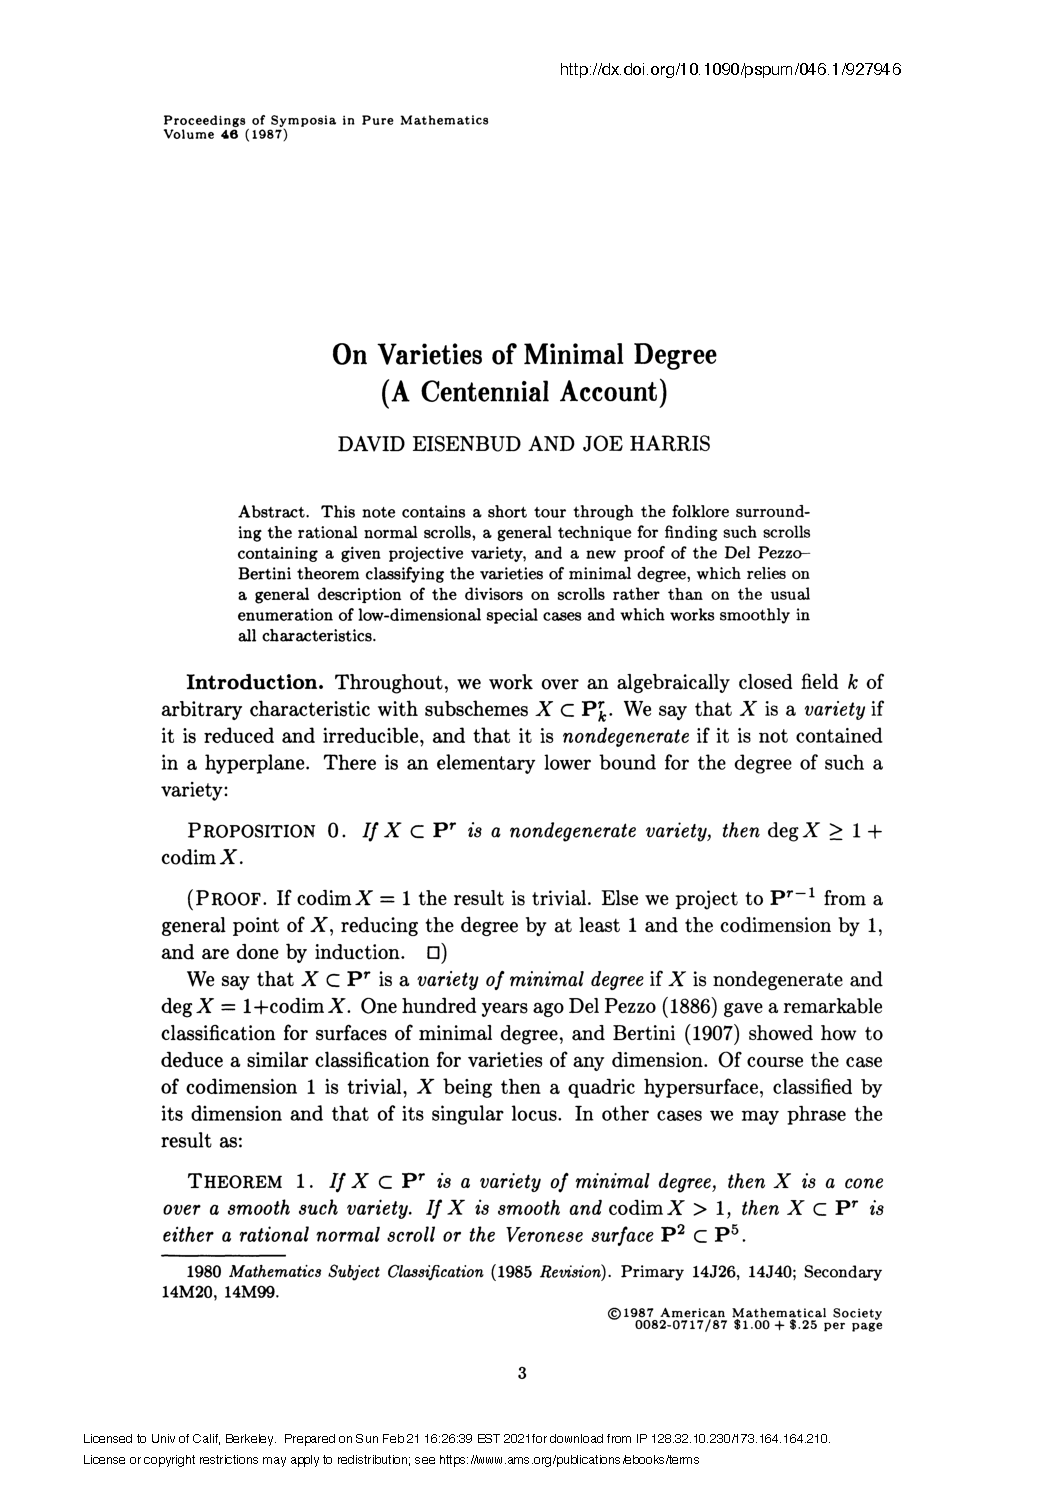
\includepdf[pages=1-11]{Centennial.pdf}

%footer for separate chapter files

\ifx\whole\undefined
%\makeatletter\def\@biblabel#1{#1]}\makeatother
\makeatletter \def\@biblabel#1{\ignorespaces} \makeatother
\bibliographystyle{msribib}
\bibliography{slag}

%%%% EXPLANATIONS:

% f and n
% some authors have all works collected at the end

\begingroup
%\catcode`\^\active
%if ^ is followed by 
% 1:  print f, gobble the following ^ and the next character
% 0:  print n, gobble the following ^
% any other letter: normal subscript
%\makeatletter
%\def^#1{\ifx1#1f\expandafter\@gobbletwo\else
%        \ifx0#1n\expandafter\expandafter\expandafter\@gobble
%        \else\sp{#1}\fi\fi}
%\makeatother
\let\moreadhoc\relax
\def\indexintro{%An author's cited works appear at the end of the
%author's entry; for conventions
%see the List of Citations on page~\pageref{loc}.  
%\smallbreak\noindent
%The letter `f' after a page number indicates a figure, `n' a footnote.
}
\printindex[gen]
\endgroup % end of \catcode
%requires makeindex
\end{document}
\else
\fi






%header and footer for separate chapter files

\ifx\whole\undefined
\documentclass[12pt, leqno]{book}
\usepackage{graphicx}
\input style-for-curves.sty
\usepackage{hyperref}
\usepackage{showkeys} %This shows the labels.
%\usepackage{SLAG,msribib,local}
%\usepackage{amsmath,amscd,amsthm,amssymb,amsxtra,latexsym,epsfig,epic,graphics}
%\usepackage[matrix,arrow,curve]{xy}
%\usepackage{graphicx}
%\usepackage{diagrams}
%
%%\usepackage{amsrefs}
%%%%%%%%%%%%%%%%%%%%%%%%%%%%%%%%%%%%%%%%%%
%%\textwidth16cm
%%\textheight20cm
%%\topmargin-2cm
%\oddsidemargin.8cm
%\evensidemargin1cm
%
%%%%%%Definitions
%\input preamble.tex
%\input style-for-curves.sty
%\def\TU{{\bf U}}
%\def\AA{{\mathbb A}}
%\def\BB{{\mathbb B}}
%\def\CC{{\mathbb C}}
%\def\QQ{{\mathbb Q}}
%\def\RR{{\mathbb R}}
%\def\facet{{\bf facet}}
%\def\image{{\rm image}}
%\def\cE{{\cal E}}
%\def\cF{{\cal F}}
%\def\cG{{\cal G}}
%\def\cH{{\cal H}}
%\def\cHom{{{\cal H}om}}
%\def\h{{\rm h}}
% \def\bs{{Boij-S\"oderberg{} }}
%
%\makeatletter
%\def\Ddots{\mathinner{\mkern1mu\raise\p@
%\vbox{\kern7\p@\hbox{.}}\mkern2mu
%\raise4\p@\hbox{.}\mkern2mu\raise7\p@\hbox{.}\mkern1mu}}
%\makeatother

%%
%\pagestyle{myheadings}

%\input style-for-curves.tex
%\documentclass{cambridge7A}
%\usepackage{hatcher_revised} 
%\usepackage{3264}
   
\errorcontextlines=1000
%\usepackage{makeidx}
\let\see\relax
\usepackage{makeidx}
\makeindex
% \index{word} in the doc; \index{variety!algebraic} gives variety, algebraic
% PUT a % after each \index{***}

\overfullrule=5pt
\catcode`\@\active
\def@{\mskip1.5mu} %produce a small space in math with an @

\title{Personalities of Curves}
\author{\copyright David Eisenbud and Joe Harris}
%%\includeonly{%
%0-intro,01-ChowRingDogma,02-FirstExamples,03-Grassmannians,04-GeneralGrassmannians
%,05-VectorBundlesAndChernClasses,06-LinesOnHypersurfaces,07-SingularElementsOfLinearSeries,
%08-ParameterSpaces,
%bib
%}

\date{\today}
%%\date{}
%\title{Curves}
%%{\normalsize ***Preliminary Version***}} 
%\author{David Eisenbud and Joe Harris }
%
%\begin{document}

\begin{document}
\maketitle

\pagenumbering{roman}
\setcounter{page}{5}
%\begin{5}
%\end{5}
\pagenumbering{arabic}
\tableofcontents
\fi


\chapter{Embeddings of Hyperelliptic and Trigonal curves}
\label{ScrollsChapter}
\section{Hyperelliptic curves}
\fix{maybe start a new Chapter?}

In our early encounters with curves, we frequently assumed that the curve we were considering was non-hyperelliptic, since the behavior of hyperelliptic curves is so atypical. In this section, we'll describe the geometry of hyperelliptic curves.

\subsection{Basic models of hyperelliptic curves}\fix{move this section to ch 2; add discussion of adjoints--- perhaps as exercises?}

We start by establishing some basic facts about hyperelliptic curves. Many of these follow from general theorems like Riemann-Roch; but since they can be established by direct examination we will carry that out here.

Suppose $C$ is a smooth, projective hyperelliptic curve of genus $g \geq 2$. By definition, $C$ admits a degree 2 map $\pi : C \to \PP^1$; and as we've observed (\ref{**}) this map is unique.

By Riemann-Hurwitz, \fix{attibution?} the map $\pi : C \to \PP^1$ will have $2g+2$ distinct simple branch points, say $\lambda_1,\dots,\lambda_{2g-2} \in \PP^1$. An open subsect $C^\circ$ of $C$ can then be realized as the smooth projective completion of the affine curve given as
$$
C^\circ = \big\{ (x,y) \in \AA^2 \; \mid \; y^2 = \prod_{i=1}^{2g+2} (x - \lambda_i) \big\}.
$$ 
\fix{if two of the $\lambda_i$ coinncide, then the curve develops a singular point. Much of what we will do carries over to the singular case.} \fix{say the smooth model has 2 points at $\infty$.} Note that if we simply take the closure of this locus in $\PP^2$, the resulting curve will be highly singular at the point $[1,0,0]$, as can be seen either  directly by making an appropriate change of variables, or by invoking the genus formula for plane curves: if the closure were smooth, it would have genus $\binom{2g+1}{2}$. We can, however, complete the curve simply in $\PP^1 \times \PP^1$, for example by setting \fix{this is a rabbit from a hat. Consider either saying that by the previous section, if there's an emb in P3 then its on P1 x P1 as a divisor of type
2,g+1; and then "finding" this embedding as below; or moving this page to the early place where hyperelliptic curves are first mentioned.}
$$
y' = \frac{y}{\prod_{i=1}^{g+1} (x - \lambda_i)};
$$
we can then write the equation of a still smaller open subset of $C$ as
$$
{y'}^2 \cdot \prod_{i=1}^{g+1} (x - \lambda_i) \; = \; \prod_{i=g+2}^{2g+2} (x - \lambda_i).
$$
If we now take the closure of this locus in $\PP^1 \times \PP^1$, we get a curve of type $(2,g+1)$ on $\PP^1 \times \PP^1$; this curve is smooth, as can be seen again either directly in coordinates or by invoking the genus formula for curves on $\PP^1 \times \PP^1$. In other words,
$$
C \; = \; V\Big(Y_0^2\cdot \prod_{i=1}^{g+1} (X_1 - \lambda_iX_0) - Y_1^2 \cdot \prod_{i=g+2}^{2g+2} (X_1 - \lambda_iX_0) \Big)
$$

Next, let's describe the space of regular differentials on $C$. For this, it's convenient to work with the affine model $C^\circ = V(f) \subset \AA^2$, where
$$
f(x,y) = y^2 - \prod_{i=1}^{2g-2} (x - \lambda_i).
$$

We'll denote the two points at infinity---that is, the two points of $C \setminus C^\circ$---as $p$ and $q$.

To start, consider the simple differential $dx\in \Omega_{C^\circ/k}$. This is clearly regular on $C^\circ$, with zeros at the ramification points $r_i = (\lambda_i, 0)$. But it does not extend to a regular differential on all of $C$: it will have double poles at $p$ and $q$, as can be seen either directly or by degree considerations: as we said, $dx$ has $2g+2$ zeros, while the degree of $K_C$ is $2g-2$, meaning that there must be poles at the points $p$ and $q$.

To kill these poles, we can of course divide by $x^2$ (or any quadratic polynomial in $x$). But that just introduces new poles in the finite part $C^\circ$ of $C$. Instead, we want to multiply $dx$ by a rational function with zeros at $p$ and $q$, but \emph{whose poles occur only at the points where $dx$ has zeroes}---that is, the points $r_i$.  A natural choice is simply the reciprocal of the partial derivative $f_y = \partial f/ \partial y = 2y$, which vanishes exactly at the points $r_i$, and has correspondingly a pole of order $g+1$ at each of the points $p$ and $q$ (reason: the involution $y\to -y$ fixes $C^\circ$ and $x$), and exchanges the points $p,q$. In other words, the differential
$$
\omega = \frac{dx}{f_y}
$$
is regular, with divisor
$$
(\omega) = (g-1)p + (g-1)q.
$$
The remaining regular differentials on $C$ are now easy to find: Since $x$ has only a simple pole
at the two points at infinity \fix{say why}. we can  multiply $\omega$ by any $x^k$ with $k = 0, 1, \dots, g-1$. Since this gives us $g$ independent differentials, these  form a basis for $H^0(K_C)$.


 1) special linear series are mult $g^1_2$+basepoints. 2) Given an embedding, there's a union of lines. If the embedding is complete, we get a matrix...that defines the union of lines. Scrolls in all dimensions as unions of spans of divisors.
 
 
\subsection{General embeddings of degree
genus$+3$} 

It's a divisor on a quadric in $\PP^{3}$ of type $(2,g+1)$


\section{Trigonal curves}

\subsection{Special linear series on trigonal curves}

In analyzing special linear series on a hyperelliptic curve, we made crucial use of the facts that the canonical image of a hyperelliptic curve is a rational normal curve, and that any collection of points on a rational normal curve $C \subset \PP^n$ either are linearly independent or span $\PP^n$. In a similar (though necessarily less complete) way, we can use the fact that the canonical image of a trigonal curve lies on a rational normal surface scroll to describe special linear series on it.

 

\begin{lemma}
Let $S = S_{a,b} \subset \PP^n$ be a rational normal surface scroll. Any hyperplane section $H \cap S$ consists of the union of a rational normal curve $E$, which is a section of the scroll, and a union of lines of the ruling of the scroll.
\end{lemma}

Note that the curve $E$ must be a reduced component of $S \cap H$, but the lines $L_i$ may coincide, i.e., may be non-reduced components of the intersection. In the following proof, we'll assume for clarity that the lines $L_i$ are distinct (that is, $S \cap H$ is reduced); we leave it as an exercise to rewrite the proof to accommodate the remaining cases.

\begin{proof}
Let $F \in \Pic(S)$ be the class of a line of the ruling. Since $F^2 = 0$ and $H\cdot F = 1$, exactly one of the components of $S \cap H$ must have intersection number 1 with $F$; all other components must have intersection number 0 with $F$ and so must be lines of the ruling.

It remains to show that the unique component $E$ of $H \cap S$ having intersection number 1 with $F$ is a rational normal curve. This can be seen directly, but there's a shortcut. Suppose that we have
$$
S \cap H = E \cup L_1 + \dots + L_k,
$$
so that in particular $\deg(E) = n-1-k$. Since each of the lines $L_i$ of the ruling must meet $C$, we have that
\begin{align*}
n-1 &= \dim(\overline{S \cap H}) \\
&\leq \dim(\overline {E}) + k\\
&\leq (n-1-k) + k \\
&= n-1.
\end{align*}
We conclude that $\dim(\overline E) = n-k-1$, and hence that $E$ is a rational normal curve.
\end{proof}

Note that if $S = S_{a,b}$ with $a \leq b$, we must have either $0 \leq k \leq a$ or $k = b$: as soon as $k > a$, the span of the lines $L_i$ will contain the directrix of the scroll, and so must consist of the union of the directrix with $n-1-a = b$ lines.

Now let $C$ be a trigonal curve of genus $g \geq 5$, embedded in $\\P^{g-1}$ as a canonical curve, and let $S$ be the scroll containing $C$. We want to describe special linear series $\cD = |D|$. If our linear series has base points, we can delete them; so we'll assume that $|D|$ and $|K-D|$ are base point free. Note that this implies that   both  $r(D) \geq 1$ and $r(K-D) \geq 1$. In addition, it follows by Bertini that a general divisor $D \in \cD$ is reduced, that is, consists of distinct points $p_1,\dots,p_d$.

Now, the first hypothesis, that $r(D) \geq 1$, says that the points $p_1,\dots,p_d$ are linearly dependent. The second hypothesis, that $r(K-D) \geq 1$, says that the points $p_i$ span a subspace of codimension at least 2 in $\PP^{g-1}$ They therefore lie on at least a pencil of hyperplanes; let $H$ be a general hyperplane containing $D$.




. is effective, says that the divisor $D$ lies in a hyperplane section $C \cap H$; let $H$ be a general such hyperplane. At the same time 

canonical image lies on a 2-dim scroll (non -subcanonical embedding only on 3-dim scrolls).  embedding of a trigonal curve lies on the same scroll.Stratification of trigonal curves by Maroni invariants. Dimensions via automorphism groups of scrolls.

\section{Castelnuovo's Theorem}
(Statement only) \fix{we'll need the existence of smooth curves in given classes --- base point freeness of certain divisor classes on the scroll. Theorem: bpf iff they meet both a,b rational normal curves positively. reference to Montreal? better to make a tex file of the essential bit and put it in, as appendix. or ACGH?}

%footer for separate chapter files

\ifx\whole\undefined
%\makeatletter\def\@biblabel#1{#1]}\makeatother
\makeatletter \def\@biblabel#1{\ignorespaces} \makeatother
\bibliographystyle{msribib}
\bibliography{slag}

%%%% EXPLANATIONS:

% f and n
% some authors have all works collected at the end

\begingroup
%\catcode`\^\active
%if ^ is followed by 
% 1:  print f, gobble the following ^ and the next character
% 0:  print n, gobble the following ^
% any other letter: normal subscript
%\makeatletter
%\def^#1{\ifx1#1f\expandafter\@gobbletwo\else
%        \ifx0#1n\expandafter\expandafter\expandafter\@gobble
%        \else\sp{#1}\fi\fi}
%\makeatother
\let\moreadhoc\relax
\def\indexintro{%An author's cited works appear at the end of the
%author's entry; for conventions
%see the List of Citations on page~\pageref{loc}.  
%\smallbreak\noindent
%The letter `f' after a page number indicates a figure, `n' a footnote.
}
\printindex[gen]
\endgroup % end of \catcode
%requires makeindex
\end{document}
\else
\fi

%header and footer for separate chapter files

\ifx\whole\undefined
\documentclass[12pt, leqno]{book}
\usepackage{graphicx}
\input style-for-curves.sty
\usepackage{hyperref}
\usepackage{showkeys} %This shows the labels.
%\usepackage{SLAG,msribib,local}
%\usepackage{amsmath,amscd,amsthm,amssymb,amsxtra,latexsym,epsfig,epic,graphics}
%\usepackage[matrix,arrow,curve]{xy}
%\usepackage{graphicx}
%\usepackage{diagrams}
%
%%\usepackage{amsrefs}
%%%%%%%%%%%%%%%%%%%%%%%%%%%%%%%%%%%%%%%%%%
%%\textwidth16cm
%%\textheight20cm
%%\topmargin-2cm
%\oddsidemargin.8cm
%\evensidemargin1cm
%
%%%%%%Definitions
%\input preamble.tex
%\input style-for-curves.sty
%\def\TU{{\bf U}}
%\def\AA{{\mathbb A}}
%\def\BB{{\mathbb B}}
%\def\CC{{\mathbb C}}
%\def\QQ{{\mathbb Q}}
%\def\RR{{\mathbb R}}
%\def\facet{{\bf facet}}
%\def\image{{\rm image}}
%\def\cE{{\cal E}}
%\def\cF{{\cal F}}
%\def\cG{{\cal G}}
%\def\cH{{\cal H}}
%\def\cHom{{{\cal H}om}}
%\def\h{{\rm h}}
% \def\bs{{Boij-S\"oderberg{} }}
%
%\makeatletter
%\def\Ddots{\mathinner{\mkern1mu\raise\p@
%\vbox{\kern7\p@\hbox{.}}\mkern2mu
%\raise4\p@\hbox{.}\mkern2mu\raise7\p@\hbox{.}\mkern1mu}}
%\makeatother

%%
%\pagestyle{myheadings}

%\input style-for-curves.tex
%\documentclass{cambridge7A}
%\usepackage{hatcher_revised} 
%\usepackage{3264}
   
\errorcontextlines=1000
%\usepackage{makeidx}
\let\see\relax
\usepackage{makeidx}
\makeindex
% \index{word} in the doc; \index{variety!algebraic} gives variety, algebraic
% PUT a % after each \index{***}

\overfullrule=5pt
\catcode`\@\active
\def@{\mskip1.5mu} %produce a small space in math with an @

\title{Personalities of Curves}
\author{\copyright David Eisenbud and Joe Harris}
%%\includeonly{%
%0-intro,01-ChowRingDogma,02-FirstExamples,03-Grassmannians,04-GeneralGrassmannians
%,05-VectorBundlesAndChernClasses,06-LinesOnHypersurfaces,07-SingularElementsOfLinearSeries,
%08-ParameterSpaces,
%bib
%}

\date{\today}
%%\date{}
%\title{Curves}
%%{\normalsize ***Preliminary Version***}} 
%\author{David Eisenbud and Joe Harris }
%
%\begin{document}

\begin{document}
\maketitle

\pagenumbering{roman}
\setcounter{page}{5}
%\begin{5}
%\end{5}
\pagenumbering{arabic}
\tableofcontents
\fi


\chapter{Hilbert Schemes}
\label{HilbertSchemesChapter}

In Chapter~\ref{}, we looked at curves of low genus and described the linear systems on them; that is, their maps to (and in particular their embeddings in) projective space. In this chapter we'll ask a more refined question: can we describe the family of all such curves in projective space?

We'll limit ourselves to looking at curves in $\PP^3$. Denote by $\cH = \cH_{dm-g+1}(\PP^3)$ the Hilbert scheme parametrizing subschemes of $\PP^3$ with Hilbert polynomial $p(m) = dm-g+1$ (which includes
curves of degree $d$ and genus $g$ in $\PP^3$), and by $\cH^\circ \subset \cH$ the open subset parametrizing smooth, irreducible, nondegenerate curves $C \subset \PP^3$. 

Two basic questions about the schemes $\cH^\circ$ are:

\begin{enumerate}
\item[$\bullet$] Is $\cH^\circ$ irreducible? and
\item[$\bullet$]  What is its dimension or dimensions?
\end{enumerate}

Of course, there are many more questions about the geometry of $\cH^\circ$: for example,  where is it singular? What is the closure $\overline{\cH^\circ} \subset \cH$ in the whole Hilbert scheme? (In other words, when is a subscheme $X \subset \PP^3$ with Hilbert polynomial $dm-g+1$ \emph{smoothable}, in the sense that it is the flat limit of a family of smooth curves?) What is the Picard group of $\cH^\circ$ or of its closure? We will for the most part not address these, though we will indicate the answers in special cases.

We will start with curves of the lowest possible degree:

\section{Degree 3}

The smallest possible degree of an irreducible, nondegenerate curve $C \subset \PP^3$ is 3. Any irreducible, nondegenerate curve $C \subset \PP^3$ of degree 3 is a twisted cubic, so that in this case $\cH^\circ$ is the parameter space for twisted cubics.

\begin{proposition}\label{hilb of twisted cubics}
The open subset $\cH^\circ$ of the Hilbert scheme $\cH_{3m+1}$ parametrizing twisted cubics is irreducible of dimension 12.
\end{proposition}

\begin{proof}  There are in fact several ways of establishing this statement. To start with the simplest, let $C_0 \subset \PP^3$ be any given twisted cubic, and consider the family of translates of $C_0$ by automorphisms $A \in \PGL_4$ of $\PP^3$: that is, the family
$$
\cC = \{ (A, p) \in \PGL_4 \times \PP^3 \; \mid \; p \in A(C_0) \}.
$$
Via the projection $\pi : \cC \to \PGL_4$, this is a family of twisted cubics, and so it induces a map
$$
\phi : \PGL_4 \to \cH^\circ.
$$
Since every twisted cubic is a translate of $C_0$, this is surjective, with fibers isomorphic to the stabilizer of $C_0$, that is, the subgroup of $\PGL_4$ of automorphisms of $\PP^3$ carrying $C_0$ to itself. Every automorphism of $C_{0}$ is induced by an automorphism of $\PP^{3}$ \fix{have we discussed this?}, so the stabilizer is isomorphic to $\PGL_2$ and  thus has dimension 3. Since $\PGL_4$ is irreducible of dimension 15, we conclude that \emph{$\cH^\circ$ is irreducible of dimension 12}.
\end{proof}

This argument is based on a rather special fact, that all irreducible nondegenerate cubic curves $C \subset \PP^3$ are translates of one another. There is another, less ad-hoc way of arriving at the conclusion above which we'll now describe. While it seem much more involved, as we'll see in the next couple of sections it's a broadly applicable technique in general.

\fix{David read to here 12-5-2020}
\begin{proof}[Second Proof] The idea behind this approach is the fact the intersection of any two distinct quadrics $Q, Q' \supset C$ containing a twisted cubic curve $C$ is the union of $C$ and a line $L \subset \PP^3$, which follows from B\' ezout's theorem. 
Conversely, suppose that $L \subset \PP^3$ is any line and  $Q, Q'$ two general quadrics containing $L$; write the intersection $Q \cap Q'$ as a union $L \cup C$. By Bertini, $Q$ is smooth, and the quadric $Q'$ will intersect it in a curve of type $(2,2)$, and so the curve $C$ will have class $(2,1)$ or $(1,2)$. Since the quadrics $Q'$ containing $L$ cut out on $Q$ the complete linear system of curves of type $(2,1)$, which has no base locus, Bertini's theorem tells us that $C$ will be smooth, so that the intersection $Q \cap Q' = L \cup C$ will be the union of $L$ and a twisted cubic. This suggests that we set up an incidence correspondence: let $\PP^9$ denote the projective space of quadrics in $\PP^3$, and consider
$$
\Phi = \{ (C, L, Q, Q') \in \cH^\circ \times \GG(1,3) \times \PP^9 \times \PP^9 \; \mid \; Q \cap Q' = C \cup L \}.
$$

We'll analyze $\Phi$ by considering the projection maps to $\cH^\circ$ and $\GG(1,3)$; that is, by looking at the diagram

\begin{diagram}
& &  \Phi & & \\
& \ldTo^{\pi_1} & & \rdTo^{\pi_2} & \\
\cH^\circ & & & & \GG(1,3)
\end{diagram}

Consider first the projection map $\pi_2 : \Phi \to \GG(1,3)$ on the second factor. By what we just said, the fiber over any point $L \in \GG(1,3)$ is an open subset of $\PP^6 \times \PP^6$, where $\PP^6$ is the space of quadrics containing $L$; it follows that $\Phi$ is irreducible of dimension $4 + 2\times 6 = 16$. Going down the other side, we see that the map $\pi_1 : \Phi \to \cH^\circ$ is surjective, with fibers open subsets of $\PP^2 \times \PP^2$; we conclude again that \emph{$\cH^\circ$ is irreducible of dimension 12}.
\end{proof}

Yet another proof of Proposition~\ref{hilb of twisted cubics} is based on a remarkable fact about twisted cubics, described in the next exercise; the application to $\cH^\circ$ is carried out in the following one.

\begin{exercise}
Show that if $p_1,\dots, p_6 \in \PP^3$ are any six points in $\PP^3$ in \emph{linear general position}, that is, with no four lying in a plane, then there exists a unique twisted cubic curve $C \subset \PP^3$ containing them.
\end{exercise}

\begin{exercise}
Consider the incidence correspondence
$$
\Phi = \{ (p_1,\dots,p_6, C) \in (\PP^3)^6 \times \cH^\circ \; \mid p_1,\dots,p_6 \in C  \}.
$$
Use the result of the preceding problem to show that $\cH^\circ$ is irreducible of dimension 12.
\end{exercise}


Note that $\cH^\circ$ is open in the Hilbert scheme $\cH = \cH_{3m+1}(\PP^3)$, but its closure is not all of $\cH$! There is a second irreducible component of $\cH$, of dimension 15. To see this, observe that any plane cubic $C \subset \PP^2 \subset \PP^3$ has Hilbert polynomial $p(m) = 3m$. If $p \in \PP^3 \setminus C$ is any point not on $C$, then, the union $C \cup \{p\}$ is a subscheme of $\PP^3$ with Hilbert polynomial $3m+1$, and so corresponds to a point of $\cH$. But the family of such subschemes has dimension 15: we have to specify a plane in $\PP^3$ (3 parameters), a cubic curve $C$ in that plane (9 parameters) and a point $p \in \PP^4$ (3 parameters). In fact, these schemes are dense in a second irreducible component $\cH'$ of $\cH$.

In general, the Hilbert scheme $\cH_{dm-g+1}(\PP^3)$ will have many components (we don't know in general how many, or what their dimensions are), few of which actually parametrize reduced, irreducible and nondegenerate curves in $\PP^3$. This is why, for the most part, we'll be restricting our attention to the closure of $\cH^\circ$. 

\begin{exercise}
Describe the intersection of the closure  of $\cH^\circ$ in $\cH_{3m+1}$ with the second component described above. In particular, show that the locus $\Sigma$ of schemes $X$ consisting of a nodal plane cubic curve $C$ with a spatial embedded point of multiplicity 1 at the node is dense in the intersection $\overline{\cH^\circ} \cap \cH'$.
\end{exercise}

\section{Linkage} \label{SLinkage}

As the second proof of Proposition~\ref{hilb of twisted cubics} suggests, when the union of two curves $C$ and $D$ forms a complete intersection we can use this fact to relate the geometry of their respective Hilbert schemes. This is a technique we'll use repeatedly in this chapter. One thing we need in order to apply it in general is a formula relating the genera of the curves $C$ and $D$, which we'll derive in this section. This is one aspect of the general theory of \emph{liaison}, or \emph{linkage}, of curves in $\PP^3$; we'll discuss this theory in detail in Chapter~\ref{SyzygiesChapter}.

In our present situation, we assume $C$ and $D \subset \PP^3$ are curves of degrees $d$ and $e$ and genera $g$ and $h$ respectively, with no common components. We assume also that the union $C \cup D$ is a complete intersection $S \cap T$ of surfaces of degrees $s$ and $t$, with $S$ smooth. In this situation, B\'ezout tells us that $d+e = st$; we want a formula similarly relating the genera $g$ and $h$ of $C$ and $D$.

To do this, we work in the Chow ring of $S$. (This is why we assume $S$ is smooth, although the treatment in Section~\ref{} will show that this hypothesis is unnecessary.) We know that the canonical bundle $K_S = \cO_S(s-4)$, so that by adjunction 
$$
2g-2 = (C\cdot C) + (K_S\cdot C) = C\cdot C + (s-4)d, 
$$
or in other words,
$$
(C \cdot C) = 2g-2 - (s-4)d.
$$
Next, since $C \cup D$ is a complete intersection of $S$ with a surface of degree $t$, we have $C + D\sim tH$, where $H$ denotes the hyperplane class on $S$; thus we have
$$
(C \cdot D) = (C \cdot (tH - C)) = td - (C \cdot C) = td - 2g + 2 + (s-4)d
$$
and similarly
$$
(D \cdot D) = (D \cdot (tH - C)) = te - td + 2g - 2 - (s-4)d.
$$
Finally, we can apply the adjunction formula to $D$ to arrive at
$$
2h - 2 = (D \cdot D) + (K_S \cdot D) = (s-4)e  + te - td + 2g - 2 - (s-4)d.
$$
Collecting terms, we can write this in the convenient form
\begin{equation}\label{linked genus formula}
h - g = \frac{s+t-4}{2}(e-d);
\end{equation}
in words, \emph{the difference between the genera of $C$ and $D$ is proportional to the difference in their degrees, with constant of proportionality $(s+t-4)/2$}. 

We will see this formula used repeatedly in this chapter, and as we indicated it will be discussed as part of the larger theory of liaison for space curves in Chapter~\ref{}. For now, you should just take a moment and reassure yourself that the right hand side of~(\ref{linked genus formula}) is indeed an integer!

%We will generalize the technique used in second proof of Proposition~\ref{hilb of twisted cubics}. Will do first for $C, D$ smooth; at the end, have discussion of full definition and theorem.
%
%To be done: First, derive formula for genus of linked curves via intersection theory of a (presumably smooth) surface containing the curves. Similarly introduce the Rao module and show that Rao modules of linked curves are dual (with a twist) via cohomology groups of line bundles on this surface and Serre duality. Unirationality of one Hilbert scheme equiv. to unirationality of the other; discussion of historical significance and ref. to result that general curves are not linked to anything simpler.
%
%References to Chapter 10, where the 
%
%Question: Is the Hilbert scheme of twisted cubics rational?
%
%\subsection{formulas for degree and genus of linked curves}
%
%\subsection{Cheerful facts: Hartshorne-Rao; smoothness of residual curve when $I_C$ generated in degree $d$ (Prop. 5.6 in 3264)}
%
%\subsection{Unirationality of Hilbert schemes}

\section{Degree 4}

Let's move on to curves $C \subset \PP^3$ of degree 4 (always assumed smooth, irreducible and nondegenerate). The first thing to observe here is that by Clifford such a curve must have genus 0 or 1; we consider these cases in turn.

\subsection{Genus 0}\label{degree 4 genus 0}

We can deal with rational quartics by a slight variant of the first method we used to deal with twisted cubics; in fact, this method will answer our question for rational curves of any degree. Specifically, a rational curve of degree 4 is the image of a map $\phi_F : \PP^1 \to \PP^3$ given by a four-tuple $F = (F_0,F_1,F_2,F_3)$ with $F_i \in H^0(\cO_{\PP^1}(4))$. The space of all such four-tuples up to scalars is a projective space of dimension $4 \times 5 - 1 = 19$; let $U \subset \PP^{19}$ be the open subset of four-tuples such that the map $\phi$ is a nondegenerate embedding. We then have a surjective map $\pi : U \to \cH^\circ$, whose fiber over a point $C$ is the space of maps with image $C$. Since any two such maps differ by an automorphism of $\PP^1$---that is, an element of $\PGL_2$---the fibers of $\pi$ are three-dimensional; we conclude that \emph{$\cH^\circ_{4m+1}$ is irreducible of dimension 16}.

As we said, the same analysis can be used on rational curves of any degree $d$: the space $U$ of nondegenerate embeddings $\PP^1 \to \PP^3$ of degree $d$ is an open subset of the projective space $\PP^{4(d+1)-1}$ of four-tuples of homogeneous polynomials of degree $d$ on $\PP^1$ modulo scalars; and the fibers of the corresponding map $U \to \cH^\circ_{dm+1}$ are copies of $\PGL_2$. This yields the

\begin{proposition}\label{dimension of rational curves}
The open set $\cH^0 \subset \cH_{dm+1}$ parametrizing smooth, irreducible nondegenerate rational curves $C \subset \PP^3$ is irreducible of dimension $4d$.
\end{proposition}

\begin{exercise}
Just to get some practice with the method of linkage, give an argument for Proposition~\ref{dimension of rational curves} in case $d=4$ along the lines of the second argument for twisted cubics.
\end{exercise}

\subsection{Genus 1}

What about genus 1? In fact, this is relatively simple: as we saw in Section~\ref{}, a quartic curve $C \subset \PP^3$ of genus 1 is the intersection of two quadric surfaces, and by the Noether-Lasker theorem every quadric containing $C$ is a linear combination of those two. Conversely, the intersection of two general quadrics in $\PP^3$ is a quartic curve of genus 1. The space of such curves is thus an open subset of the Grassmannian $G(2,10) = \GG(1,9)$, and we conclude that \emph{$\cH^\circ_{4m}$ is irreducible of dimension 16}.

\section{Degree 5}

Let $C \subset \PP^3$ be a smooth, irreducible, nondegenerate quintic curve of genus $g$. To start with, we can use Clifford plus Riemann-Roch to bound the genus of $C$: by Clifford, the bundle $\cO_C(1)$ must be nonspecial, and then by Riemann-Roch we must have $g \leq 2$.

Now, we have already seen that the space $\cH^\circ_{5m+1}$ of rational quintic curves is irreducible of dimension 20. We'll consider, accordingly, the two remaining cases, $g=1$ and $g=2$.

\subsection{Genus 2}

We start with genus 2, since this is a case we've considered already in Section~\ref{}.  To recap the analysis, let $C \subset \PP^3$ be a smooth, irreducible, nondegenerate curve of degree 5 and genus 2. Since $h^0(\cO_C(2)) = 10-2+1 = 9$ by Riemann-Roch, the restriction map
$$
H^0(\cO_{\PP^3}(2)) \to H^0(\cO_C(2))
$$
must have a kernel; by B\'ezout, this kernel must be one-dimensional, that is, $C$ lies on a unique quadric surface $Q$. Similarly, the restriction map
$$
H^0(\cO_{\PP^3}(3)) \to H^0(\cO_C(3))
$$
must have at least a 6-dimensional kernel; since at most 4 of these are of the form $LQ$ for $L$ a linear form, we see that $C$ lies on a cubic surface not containing $Q$. Thus we can say that $C$ is residual to a line in the complete intersection of a quadric and a cubic surface, or, if $Q$ is smooth, in terms of the isomorphism $Q \cong \PP^1 \times \PP^1$ we can say $C$ is a curve of type $(2,3)$ on the quadric $Q$. Note that conversely if $L \subset \PP^3$ is a line and $Q$ and $S \subset \PP^3$ are general quadric and cubic surfaces containing $L$, and if we write
$$
Q \cap S = L \cup C
$$ 
then the curve $C$ is a curve of type $(2,3)$ on the quadric $Q$ and hence a quintic of genus 2.

This suggests two ways of describing the family $\cH^\circ$ of all such curves. First, we can use the fact that $C$ is linked to a line in much the same way we did in the case of twisted cubics: we set up an incidence correspondence
$$
\Psi = \{ (C, L, Q, S) \in \cH^\circ \times \GG(1,3) \times \PP^9 \times \PP^{19} \; \mid \; Q \cap S = C \cup L \},
$$
where the $\PP^9$ (respectively, $\PP^{19}$) is the space of quadric (respectively, cubic) surfaces in $\PP^3$. Given a line $L \in \GG(1,3)$, the space of quadrics containing $L$ is a $\PP^6$, and the space of cubics containing $L$ is a $\PP^{15}$; thus the fiber of the projection $\pi_2 : \Psi \to \GG(1,3)$ over $L$ is an open subset of $\PP^6 \times \PP^{15}$, and we see that \emph{$\Psi$ is irreducible of dimension $4 + 6 + 15 = 25$}.

Going back down the other way, the fiber of $\Psi$ over a point $C \in \cH^\circ$ is an open subset of the $\PP^5$ of cubics containing $C$; and we conclude that \emph{$\cH^\circ$ is irreducible of dimension $20$}.

Another, in some ways more direct, approach would be to use the fact that the quadric surface $Q$ containing a quintic curve $C \subset \PP^3$ of genus 2 is unique. We thus have a map
$$
\cH^\circ \to \PP^9,
$$
whose fiber over a point $Q \in \PP^9$ is the space of quintic curves of genus 2 on $Q$. 

The problem is, the space of quintic curves of genus 2 on a given quadric $Q$ is not in general irreducible: if $Q$ is smooth, it consists of the disjoint union of two $\PP^{11}$s (or rather open subsets of these $\PP^{11}$s), corresponding to the families of curves of type $(2,3)$ and $(3,2)$. Thus we can conclude immediately that $\cH^\circ$ is of pure dimension 20; but to conclude that it's irreducible we need to verify that, in the family of all smooth quadric surfaces, the monodromy exchanges the two rulings. This is not hard: it amounts to the assertion that the family
$$
\Gamma = \{ (Q,L) \in \PP^9 \times \GG(1,3) \; \mid \; L \subset Q \}
$$
is irreducible, which can be seen readily via projection on the second factor.

There is another approach to the problem of describing $\cH^\circ$, which is to describe such curves parametrically rather than via the equations defining them as subsets of $\PP^3$, which is a direct generalization of the approach we took to the proof of Proposition~\ref{dimension of rational curves} above. We'll describe this in general in Section~\ref{estimating dim hilb}. It covers the case of quintics of genus 1, so we won't deal with that case separately, except in the form of an exercise:

\begin{exercise}
Show that a smooth, irreducible, nondegenerate curve $C \subset \PP^3$ of degree 5 and genus 1 is residual to a rational quartic in the complete intersection of two cubics, and use the result of subsection~\ref{degree 4 genus 0} to deduce that the space of genus 1 quintics is irreducible of dimension 20.
\end{exercise}

\section{Degree 6}

Moving on to curves of degree 6, the first question to ask would be: what are the possible genera of smooth, irreducible, nondegenerate curves $C \subset \PP^3$ of degree 6? Once more (and for the last time, we're afraid) Clifford and Riemann-Roch suffice to answer this: if the line bundle $\cO_C(1)$ is nonspecial, then by Riemann-Roch we have $g \leq 3$; and if $\cO_C(1)$ is special, $d \leq 2g-2$ and hence $g \leq 4$.

The cases of general 0, 1 and 2 are covered under Proposition~\ref{nonspecial Hilbert}, leaving us the cases $g = 3$ and 4. Both are well-handled by the Cartesian approach of describing their ideals; we'll start with the relatively simple case of $g=4$.

\subsection{Genus 4}

This is easy: by Riemann-Roch, a curve of degree 6 and genus 4 in $\PP^3$ is necessarily a canonical curve, and as we've seen a canonical curve of genus 4 is the complete intersection of a (unique) quadric $Q$ and a cubic surface $S$. We thus have a map
$$
\alpha : \cH^\circ \rTo \PP^9
$$
sending a curve $C$ to the quadric $Q$ containing it. Moreover, the fibers of this map are open subsets of the projective space $\PP V$, where $V$ is the quotient
$$
V = \frac{H^0(\cO_{\PP^3}(3))}{H^0(\cI_{Q/\PP^3}(3))}
$$
of the space of all cubic polynomials modulo cubics vanishing on $Q$. Since this vector space has dimension 16, the fibers of $\alpha$ are irreducible of dimension 15, and we deduce that \emph{the space $\cH^\circ_{6m-3}$ is irreducible of dimension 24}.

\subsection{Genus 3}

\begin{exercise}
Let $C$ be a curve of degree 6 and genus 3, and assume that $C$ does not lie on any quadric surface. Show that $C$ is residual to a twisted cubic in the complete intersection of two cubic surfaces, and use this to deduce that the space of such curves is irreducible of dimension 24.
\end{exercise}


\begin{exercise}
Now let $C$ again be a curve of degree 6 and genus 3, but now assume that $C$ \emph{does} lie on a quadric surface $Q$. Show that such a curve is a specialization/flat limit of curves of the type described in the last exercise, and conclude that $\cH^\circ_{6m-2}(\PP^3)$ is irreducible of dimension 24.
\end{exercise}


\begin{exercise}
For another approach, try tweaking the argument for Proposition~\ref{nonspecial Hilbert} to cover the case $d=2g$, and use this to deduce again that $\cH^\circ_{6m-2}(\PP^3)$ is irreducible of dimension 24.
\end{exercise}

\section{Why  $4d$?}\label{estimating dim hilb}

The sharp-eyed reader will have noticed that, in every case analyzed so far, the dimension of the Hilbert scheme parametrizing smooth curves of degree $d$ and genus $g$ in $\PP^3$ is $4d$. While this is not the case in general (we will see shortly an example where it fails), the persistence of $4d$ suggests that there may be a way of estimating the dimension of the Hilbert scheme that yields, in the case of curves in $\PP^3$, the ``expected" dimension $4d$.

In fact, there are two, and in the following subsections we'll describe both approaches. For the remainder of this section, we will step outside $\PP^3$ and consider the restricted Hilbert scheme $\cH^\circ$ of smooth, irreducible, nondegenerate curves in $\PP^r$.

\subsection{Estimating $\dim \cH^\circ$ by Brill-Noether}

Our first approach to the problem of estimating the dimension of $\cH^\circ$ is a direct generalization of the approach we took to the proof of Proposition~\ref{dimension of rational curves} above, with two additional wrinkles. Since not all line bundles of degree $d$ on a curve $C$ of genus $g > 0$ are linearly equivalent, this will involve involve invoking the Picard variety $\Pic_d(C)$ parametrizing line bundles of degree $d$ on a given curve $C$, discussed in Chapter~\ref{new Jacobians chapter}; and since not all curves of genus $g > 0$ are isomorphic, it will similarly involve the moduli space  $M_g$ parametrizing abstract curves of genus $g$, discussed in Chapter~\ref{Moduli chapter}.

To set this up, again let $\cH^\circ$ be the space of smooth, irreducible, nondegenerate curves $C \subset \PP^3$ of degree 5 and genus 2. By forgetting the information of the particular embedding of $C$ in $\PP^3$ and remembering only the isomorphism class of $C$, we have a map
$$
\mu : \cH^\circ \rTo M_2.
$$
What does the fiber $\Sigma_C =\mu^{-1}(C)$ of the map $\mu$ over a point $C \in M_2$ look like? To start, we have a map
$$
\nu : \Sigma_C \rTo \Pic_5(C),
$$
obtained by sending a point in $\Sigma_C$ to the line bundle $\cO_C(1)$. Moreover, by Proposition~\ref{**}, which says that any line bundle of degree 5 on a curve of genus 2 is very ample, this map is surjective. Finally, the fiber of $\nu$ over a point $\cL \in \Pic_5(C)$ is simple to describe: once we've specified the abstract curve $C$, and the line bundle $\cL \in \Pic_5(C)$ giving the embedding, since $h^0(\cL) = 4$ all we have to do is to choose a basis for $H^0(\cL)$ up to scalars. In other words, the fiber of $\nu$ are isomorphic to $\PGL_4$. We can now work our way up from $M_2$:

\begin{enumerate}

\item[$\bullet$] We know (or at least have asserted) that $M_2$ is irreducible of dimension 3.

\item[$\bullet$] It follows that the space of pairs $(C,\cL)$ with $C \in M_2$ a smooth curve of genus 2 and $\cL \in \Pic_5(C)$ is irreducible of dimension 3 + 2 = 5; and finally

\item[$\bullet$] It follows that $\cH^\circ$ is irreducible of dimension $5 + 15 = 20$.

\end{enumerate}

In fact, this approach applies to a much wider range of examples: whenever $d \geq 2g+1$ and $r \leq d-g$, we can look at the tower of spaces

\begin{diagram}
\cH^\circ = \cH^\circ_{dm-g+1}(\PP^r) \\
\dTo \\
\cP_{d,g} = \{(C,\cL) \mid \cL \in \Pic_d(C) \} \\
\dTo \\
M_g.
\end{diagram}

Exactly as in the special case $(d,g,r) = (5,2,3)$ above, we can work our way up the tower:


\begin{enumerate}

\item[$\bullet$]  $M_g$ is irreducible of dimension $3g-3$;

\item[$\bullet$] it follows that $\cP_{d,g}$ is irreducible of dimension $3g-3+g = 4g-3$; and finally

\item[$\bullet$] since the fibers of $\cH^\circ \to \cP_{d,g}$ consist of $(r+1)$-tuples of linearly independent sections of $\cL$ (mod scalars), it follows that $\cH^\circ$ is irreducible of dimension $4g-3 + (r+1)(d-g+1) - 1$.

\end{enumerate}

In sum, we have the

\begin{proposition}\label{nonspecial Hilbert}
Whenever $d \geq 2g+1$, the space $\cH^\circ$ of smooth, irreducible, nondegenerate curves $C \subset \PP^r$ is either empty (if $d-g < r$) or irreducible of dimension $4g-3 + (r+1)(d-g+1) - 1$.
\end{proposition}

Note that in case $r=3$, this reduces to $4d$. Note also that we can modify this analysis to extend this beyond the range $d \geq 2g+1$: as long as the Brill-Noether number $\rho(d,g,r) \geq 0$, the Brill-Noether theorem tells us that for a general curve $C$, the variety $W^r_d(C)$ has dimension $\rho$, and (assuming $r \geq 3$) the general point of $W^r_d(C)$ corresponds to a very ample line bundle wirth exactly $r+1$ sections. In this situation, there is a unique component of $\cH_0 \subset \cH^\circ$ dominating $M_g$, and the map $\cH^\circ \to \cP_{d,g}$ carries this component to a subvariety $\cW^r_d \subset \cP_{d,g}$ of dimension $3g-3 + \rho$; we have then
$$
\dim \cH_0 = 3g-3+\rho + (r+1)^2 - 1 = 4g-3 + (r+1)(d-g+1) - 1,
$$
extending the calculation of Proposition~\ref{nonspecial Hilbert}. The component $\cH_0$ is called the \emph{principal component} of the Hilbert scheme; there may be others as well, of possibly different dimension, and we do not know precisely for which $d,g$ and $r$ these occur.

\subsection{Estimating $\dim \cH^\circ$ by Euler characteristic of the normal bundle}

It's interesting to compare the estimate of  $\dim \cH^\circ$ above with what we get via a completely different approach. To set this up, let $\cH$ be a component of the scheme $\cH^\circ$, with $C \subset \PP^r$ a curve corresponding to a general point $[C]$ of $\cH$.

We start with the idea that the dimension of the scheme $\cH$ is approximated by the dimension of its Zariski tangent space $T_{[C]}\cH$ at a general point $[C]$. But we've seen that the tangent space to $\cH$ at $[C]$ is the space $H^0(\cN_{C/\PP^r})$ of global sections of the normal bundle $\cN = \cN_{C/\PP^r}$. And we can think of the dimension $h^0(\cN)$ as approximated by the Euler characteristic $\chi(\cN)$, with ``error term" $h^1(\cN)$ coming from its first cohomology group.

Given these two approximations, we arrive at a number we can actually compute! From the exact sequence
$$
0 \to T_C \to T_{\PP^r}|_C \to \cN \to 0
$$
we deduce that
\begin{align*}
c_1(\cN) &= c_1(T_{\PP^r}|_C) - c_1(T_C) \\
&= (r+1)d - (2-2g).
\end{align*}

Now we can apply the Riemann-Roch formula for vector bundles on curves (\cite{3264}) to conclude that
\begin{align*}
\chi(\cN) &= c_1(\cN) - \rank(\cN)(g-1) \\
&= (r+1)d - (r-3)(g-1).
\end{align*}

Note that our two ``estimates" are actually inequalities. But, unfortunately, they go in opposite directions: we have
$$
\dim \cH \leq \dim T_{[C]}\cH,
$$
but 
$$
\dim T_{[C]}\cH \geq \chi(\cN).
$$


\subsection{They're the same!} Proposition~\ref{nonspecial Hilbert} suggests that the ``expected dimension" of the restricted Hilbert scheme $\cH^\circ$ of curves of degree $d$ and genus $g$ in $\PP^r$ should be 
$$
h(g,r,d) = 4g-3 + (r+1)(d-g+1) - 1.
$$
But the calculation immediately above suggests it should be $(r+1)d - (r-3)(g-1)$. Which is it? The answer is both: they're the same number!

\fix{At this point, I'd like to close out this chapter of examples of Hilbert schemes conforming to the dimension estimate of Brill-Noether, and start a new chapter, in which we go in the opposite direction and describe examples of Hilbert schemes that don't. The idea would be to give the examples below, and then finish with the conjecture that ``Brill-Noether holds in low codimension in $M_g$."} 

\section{Degree 8}

At this point, the reader may be growing impatient: in every case dealt with so far, the space $\cH^\circ_{dm-g+1}$ is irreducible of dimension $4d$. Is that the case in general?

The answer is very much no: in general, neither the number of irreducible components of $\cH^\circ_{dm-g+1}$, nor their dimensions, are known. In this section and the next we'll give the first two examples where $\cH^\circ_{dm-g+1}$ is either reducible, or of dimension $>4d$.

The first example occurs in degree 8: specifically, we consider the space $\cH^\circ = \cH^\circ_{8m-8}(\PP^3)$ of smooth, irreducible, nondegenerate curves of degree 8 and genus 9. To describe such curves $C \subset \PP^3$, we look first at the restriction map
$$
\rho_2 : H^0(\cO_{\PP^3}(2)) \rTo H^0(\cO_C(2)).
$$
The space on the left has dimension 10, as always. As for the space on the right, Riemann-Roch is ambivalent: it says that
\begin{align*}
h^0(\cO_C(2)) =
\begin{cases}
9, \quad &\text{if } \cO_C(2) \cong K_C; \\
8,  \quad &\text{if } \cO_C(2) \not\cong K_C.
\end{cases}
\end{align*}

In the latter case, $C$ would have to lie on two distinct quadrics, which would violate B\'ezout; we deduce that we must have $\cO_C(2) \cong K_C$, and hence $C$ lies on a unique quadric surface $Q$.

What about cubics and higher degree surfaces? For cubics, there is no question: since $C$ lies on a (necessarily irreducible) quadric $Q$, by B\'ezout it cannot lie on any cubic not containing $Q$. Moving on to quartics, we look again at the restriction map
$$
\rho_4 : H^0(\cO_{\PP^3}(4)) \rTo H^0(\cO_C(4)).
$$
The dimensions here are, respectively, 35 and $4\cdot 8 - 9 + 1 = 24$; and we deduce that $C$ lies on at least an 11-dimensional vector space of quartic surfaces. On the other hand, only a 10-dimensional vector subspace of these consist of quartics vanishing on Q; and so we conclude that \emph{$C$ lies on a quartic surface not containing $Q$}. Next, B\'ezout tells us that we must have $C = Q \cap S$, and the Noether-Lasker theorem tells us that the equations of $Q$ and $S$ generate the homogeneous ideal of $C$; that is, $\ker(\rho_4)$ has dimension exactly 11, and so $S$ is unique modulo quartics vanishing on $Q$.

What can we say about the space $\cH^\circ$ parametrizing such curves? Well, we have a natural map $\cH^\circ \to \PP^9$ with dense image; and the fibers, by what we've just said, is an open subset of the projective space $\PP V$, where $V$ is the 25-dimensional vector space
$$
V = \frac{H^0(\cO_{\PP^3}(4))}{H^0(\cI_{Q/\PP^3}(4))}.
$$
It follows that \emph{the space $\cH^\circ_{8m-8}(\PP^3)$ is irreducible of dimension 33}---one larger than the expected $4d$.


\section{Degree 9}

For the next example, consider the space $\cH^\circ = \cH^\circ_{9m-9}(\PP^3)$ of curves of degree 9 and genus 10. Once more, to describe such curves we look to the restriction maps $\rho_m$; and again, we have an ambiguity coming from Riemann-Roch, which tells us that
\begin{align*}
h^0(\cO_C(2)) =
\begin{cases}
10, \quad &\text{if } \cO_C(2) \cong K_C \; \text{(``the first case,") and } \\
9,  \quad &\text{if } \cO_C(2) \not\cong K_C  \; \text{(``the second case.")}
\end{cases}
\end{align*}
Unlike the last case, however, both are possible; we'll analyze each of these cases in turn.

1. Suppose first that $C$ does not lie on any quadric surface (so that we are necessarily in the first case above). We consider next the map $\rho_3 : H^0(\cO_{\PP^3}(3)) \to H^0(\cO_C(3))$. By Riemann-Roch, the dimension of the target is $3\cdot 9 - 10 + 1 = 18$, from which we conclude that $C$ lies on at least a pencil of cubic surfaces. Since $C$ lies on no quadrics, all of these cubic surfaces must be irreducible, and it follows by B\'ezout that the intersection of two such surfaces is exactly $C$. At this point, Noether-Lasker assures us that $C$ lies on exactly two cubics.

The space of curves of this type is thus an open subset of the Grassmannian $G(2,20)$ of pencils of cubic surfaces, which is irreducible of dimension 36.

2. Next, suppose that $C$ does lie on a quadric surface. In this case, we claim that $C$ must be a curve of type $(3,6)$, or equivalently $C$ is residual to three skew lines in the complete intersection of a quadric $Q$ and a sextic surface $S$.

In sum, there are two types of smooth, irreducible, nondegenerate curves $C \subset \PP^3$ of degree 9 and genus 10: type 1, which are complete intersections of two cubics; and type 2, which are curves of type $(3,6)$ on a quadric surface. Moreover, the family of curves of each type is irreducible of dimension 36; and we conclude that \emph{the space $\cH^\circ_{9m-9}(\PP^3)$ is reducible, with two components of dimension 36}.


\begin{exercise}
In the preceding argument, we used a dimension count to conclude that a general curve of type 1 could not be a specialization of a curve of type 2, and vice versa. Prove these assertions directly: specifically, argue that
\begin{enumerate}
\item by upper-semicontinuity of $h^0(\cI_{C/\PP^3}(2))$, argue that a curve $C$ not lying on a quadric cannot be the specialization of curves $C_t$ lying on quadrics; and
\item show that for a general curve of type $(3,6)$ on a quadric, $K_C \not\cong \cO_C(2)$, and deduce that a general curve of type 2 is not a specialization of curves of type 1.
\end{enumerate}
\end{exercise}

\begin{exercise}
Let $\Sigma_1$ and $\Sigma_2 \subset \cH^\circ_{9m-9}(\PP^3)$ be the loci of curves of types 1 and 2 respectively. 
\begin{enumerate}
\item What is the intersection of the closures of $\Sigma_1$ and $\Sigma_2$ in $\cH_{9m-9}(\PP^3)$?
\item What is the intersection of the closures of $\Sigma_1$ and $\Sigma_2$ in the whole Hilbert scheme $\cH_{9m-9}(\PP^3)$?
\end{enumerate}
\end{exercise}

\section{Two open problems}

\subsection{Brill-Noether in low codimension}

If we ignore the finer points of the Brill-Noether theorem and focus just on the statement about the dimension and irreducibility of the variety of linear series on a curve, we can express it in a simple form: Brill-Noether says that \emph{Any component of the Hilbert scheme $\cH^\circ$ of curves of degree $d$ and genus $g$ that dominates the moduli space $M_g$ has the expected dimension 
$$
h(g,r,d) = 4g-3 + (r+1)(d-g+1) - 1 = (r+1)d - (r-3)(g-1)
$$
 as calculated in Section~\ref{estimating dim hilb} above}.
 
 
Now, we've just seen an example of a component of the Hilbert scheme violating this dimension estimate, and it's not hard to produce lots of similar examples: components of the Hilbert scheme that parametrize complete intersections, or more generally determinantal curves, have in general dimension larger than the Hilbert number $h(g,r,d)$, and the following exercise gives a way of generating many more.

\begin{exercise}
Let $\cH^\circ$ be a component of the Hilbert scheme parametrizing curves of degree $d$ and genus $g$ in $\PP^3$ that dominates the moduli space $M_g$. For $s, t \gg d$, let $\cK^\circ$ be the family of smooth curves residual to a curve $C \in  \cH^\circ$ in a complete intersection of surfaces of degrees $s$ and $t$.
\begin{enumerate}
\item Show that $\cK^\circ$ is open and dense in a component of the Hilbert scheme of curves of degree $st-d$ and the appropriate genus.
\item Calculate the dimension of $\cK^\circ$, and in particular show that it is strictly greater than $h(g,r,d)$.
\end{enumerate}
\end{exercise}

So it may seem that the issue is settled: components of the Hilbert scheme dominating $M_g$ have the expected dimension; others don't in general. But there is an observed phenomenon that suggests more may be true: that \emph{components of $\cH^\circ$ whose image in $M_g$ have low codimension do have the expected dimension $h(g,r,d)$}. 

The first two cases of this are known. In~\cite{Eisenbud-Harris}, it's shown that if $\Sigma \subset M_g$ is any subvariety of codimension 1, then the curve $C$ corresponding to a general point of $\Sigma$ has no linear series with Brill-Noether number $\rho < -1$; and Edidin in ~\cite{Edidin} proves the analogous (and much harder) result for subvarieties of codimension 2. Indeed, looking over all known examples of components of the Hilbert scheme whose dimension is strictly greater than the expected $h(g,r,d)$, there are none whose image in $M_g$ has codimension less than $g-4$. We could therefore make the conjecture:

\begin{conjecture}
If $\cK \subset \cH^\circ$ is any component of the restricted Hilbert scheme, and the image of $\cK$ in $M_g$ has codimension $\leq g-4$, then $\dim \cK = h(g,r,d)$.
\end{conjecture}

The condition the image of $\cK$ in $M_g$ has codimension $\leq g-4$ is not based on any theoretical considerations, just a lack of counterexamples. It seems, accordingly, that we should be less specific: maybe conjecture, instead, just that there is a function $\lambda(g)$, with $\lim \frac{\lambda(g)}{g} > 0$, such that any component of the restricted Hilbert scheme whose image of $\cK$ in $M_g$ has codimension $\leq \lambda(g)$ has dimension $\dim \cK = h(g,r,d)$. But this is so vague as to be non-falsifiable.

\subsection{Rigid curves} Most of Brill-Noether theory, and the theory of linear systems on curves in general, centers on the behavior of linear series on a general curve. But, having opened the can of worms that is linear series on special curves, let's take a moment and go all the way to the opposite end of the spectrum.

The questions we want to raise first are simple ones to ask. As usual, let $\cH^\circ_{d,g,r}$ be the open subset of the Hilbert scheme parametrizing smooth, irreducible and nondegenerate curves of degree $d$ and genus $g$ in $\PP^r$, and let $\tilde M^r_{g,d} \subset M_g$ be the closure of the image of the map $\phi : \cH^\circ_{d,g,r}\to M_g$. We ask:
\begin{enumerate}
\item What is the smallest possible dimension of $\cH^\circ_{d,g,r}$? \; and
\item What is the smallest possible dimension of $\tilde M^r_{g,d}$?
\item Modifying the last question slightly, let $M^r_{g,d} \subset M_g$ be the closure of the locus of curves $C$ that possess a $g^r_d$ (in other words, we are dropping the condition that the $g^r_d$ be very ample), we can ask what is the smallest possible dimension of $M^r_{g,d}$?
\end{enumerate}

In other words, we are asking, ``What are the most special curves, from the point of view of linear series?" Your first thought might be, ``hyperelliptic curves," but they're not that special: the locus in $M_g$ of hyperelliptic curves has dimension $2g-1$. What about smooth plane curves? That's better -- in the sense that the locus in $M_g$ of smooth plane curves has dimension asymptotic to $g$, as the following exercise will show -- but there are still a lot of them.

\begin{exercise}
\begin{enumerate}
\item Let $C \subset \PP^2$ be a smooth plane curve of degree $d$. Show that the $g^2_d$ cut by lines on $C$ is unique; that is, $W^2_d(C)$ consists of one point.
\item Using this, find the dimension of the locus of smooth plane curves in $M_g$.
\end{enumerate}
\end{exercise}

Can we do better?  

\begin{exercise}
Using upper-semicontinuity of cohomology, prove that a deformation of a complete intersection curve $C \subset \PP^r$ is again a complete intersection; that is, complete intersection curves are dense in an irreducible component of the Hilbert scheme.
\end{exercise}                                                                                                                                                                                                                                                                                                                                                                                                                                                                                                                                                                                                                                                         

 

\section{Degree 14: the training wheels come off}

We have seen, in the last two sections, examples of Hilbert schemes of smooth curves that are reducible or of greater than the expected dimension. In this final section, we'll see an example of yet another phenomenon: a component of the Hilbert scheme that is everywhere nonreduced. 

We should say at the outset that this analysis, while not requiring ideas or techniques beyond those introduced above, does involve a substantial amount of verification and case-checking. In the interests of maintaining a reasonable flow, we have relegated many of these verifications to the exercises.

To fix the numerical invariants: we are going to be analyzing here the open subscheme $\cH^\circ$ of the Hilbert scheme parametrizing smooth, irreducible curves of degree 14 and genus 24 in $\PP^3$. As we'll see, there are three irreducible components of this locus. 

We start our analysis in the by now familiar way: we ask, given a smooth, irreducible curve $C \subset \PP^3$ of degree 14 and genus 24, what sort of surfaces may contain it? By applying the genus formula for plane curves and curves on quadrics we see right off the bat that $C$ cannot lie on a quadric, so we start our usual chart in degree 3:

\begin{center}\label{postulation table}
\begin{tabular}{ c | c | c }
 $m$ & $h^0(\cO_C(m))$ & $h^0(\cO_{\PP^3}(m))$ \\
 \hline
 3 & 19, 20 or 21 & 20 \\
 4 & 33 & 35 \\
 5 & 47 & 56 \\
 6 & 61 & 84
\end{tabular}
\end{center}

Here we see from degree considerations that $\cO_C(m)$ is nonspecial for $m \geq 4$, so Riemann-Roch gives an exact value of $h^0(\cO_C(m))$ in those cases. For $m=3$, on the other hand, the degree of $K_C(-3)$ is 4, and so 
$$
h^1(\cO_C(3)) = h^0(K_C(-3)) = 0, 1 \text{ or } 2.
$$
(The curve $C$ cannot be hyperelliptic, since it's embedded in $\PP^3$ by a special linear series, and as we saw in Chapter~\ref{} a special linear series on a hyperelliptic curve can never be very ample; thus by Clifford $h^0(K_C(-3))$ cannot be 3 or more.) Riemann-Roch thus gives three a priori possible values for $h^0(\cO_C(3))$. In particular, as far as the table is concerned $C$ may or may not lie on a cubic surface; we'll consider these cases in turn.

\subsection{Case 1: $C$ does not lie on a cubic surface}

In this case, the table says that $C$ lies on at least two linearly independent quartic surfaces $S$ and $S'$; and since $C$ does not lie on any surface of smaller degree, neither can be reducible. It follows that the intersection $S \cap S'$ must consist of the union of the curve $C$ and a curve $D$ of degree 2; and the linkage formula~(\ref{linked genus formula}) says that
$$
g(C) - g(D) = (14 - 2)\frac{4+4-4}{2} = 24,
$$
so $D$ has arithmetic genus 0. It follows that $D$ must be a plane conic curve (****); so we see that in this case $C$ is residual to a plane conic curve $D$ in the complete intersection of two quartics. Conversely, if $C$ is any curve residual to a conic curve $D$ in the complete intersection of two quartics, it must have degree 14 and genus 24, and by B\'ezout it cannot lie on a cubic surface, so it must be of this type. We can thus describe the family of all smooth curves of degree 14 and genus 24 not lying on a cubic surface via the incidence correspondence
$$
\Phi = \{ (C, D, S, S') \in \cH^\circ \times \cH_D \times \PP^{34} \times \PP^{34} \mid S \cap S' = C \cup D\}.
$$
where $\cH_D$ denotes the Hilbert scheme of plane conics. The Hilbert scheme $\cH_D$ is irreducible of dimension 8; and for any conic $D$ the space of quartic surfaces containing it is a linear subspace of $\PP^{34}$ of codimension 9. The fibers of $\Phi$ over $\cH_D$ are thus open subsets of $\PP^{25} \times \PP^{25}$, and we deduce that \emph{$\Phi$ is irreducible of dimension 58}. 

Finally, if $C$ is a curve of degree 14 and genus 24 residual to a conic $D$ in the intersection of two quartic surfaces, we see from the derivation of the linkage formula that $(C\cdot D) = 10$. It follows that any quartic surface containing $C$ must contain $D$ as well, and so by Lasker-Noether must be a linear combination of $S$ and $S'$. The fibers of $\Phi$ over its image in $\cH_C$ are thus open subsets of $\PP^1 \times \PP^1$, and we have established the

\begin{proposition}
The locus in $\cH^\circ$ of curves not lying on a cubic surface is irreducible of dimension 56.
\end{proposition} 

Since the condition of not lying on a cubic surface is open, this locus forms an irreducible component of $\cH^\circ$, which we'll call $\cH_1$.

Before we go on to Case 2, let's establish one more fact about the geometry of $\cH_1$: that it is generically smooth. To do this, we have to find the dimension of its Zariski tangent space at a general point $[C]$; that is, the dimension $h^0(\cN_{C/\PP^3})$ of the space of global sections of the normal bundle of $C$ in $\PP^3$.

To do this, we choose a quartic surface $S$ containing $C$, and consider the standard exact sequence for the normal bundle $\cN_{C/\PP^3}$:
$$
0 \to \cN_{C/S} \to \cN_{C/\PP^3} \to \cN_{S/\PP^3}|_C \to 0
$$
The bundle $\cN_{S/\PP^3}|_C \cong \cO_C(4)$, which as we've seen is nonspecial; we have $h^0(\cO_C(4)) = 33$ and $h^1(\cO_C(4)) = 0$. As for the bundle $\cN_{C/S}$,  since $S$ has trivial canonical bundle adjunction tells us that $\cN_{C/S} \cong K_C$, so we have $h^0(\cN_{C/S}) = 24$ and $h^1(\cN_{C/S}) = 1$.

This leaves two possibilities for the dimension $h^0(\cN_{C/\PP^3})$: 56 and 57. To say which occurs, we have to observe a key fact: \emph{a general quartic surface does not contain any conic curves}. In fact, there is an infinitesimal version of this: if $S$ is a smooth quartic surface containing a conic curve $C$, there exist first-order deformations of $S$ containing no first-order deformations of $C$. What this says is that the map
$H^0(\cN_{C/\PP^3}) \to H^0(\cN_{S/\PP^3}|_C)$ cannot be surjective; it follows that the coboundary map $H^0(\cN_{S/\PP^3}|_C) \to H^1(\cN_{C/S})$ must be surjective and we have
$$
h^1(\cN_{C/\PP^3}) = 0 \quad \text{and} \quad h^0(\cN_{C/\PP^3}) = 56,
$$
showing that $\cH_1$ is smooth at $[C]$.

\begin{exercise}
Let $\PP^{34}$ be the space of quartic surfaces in $\PP^3$ and $\cH = \cH^\circ_{2m+1}$ the space of conic plane curves in $\PP^3$, and consider the standard incidence correspondence
$$
\Phi = \{(S,D) \in \PP^{34} \times \cH \mid D \subset S \}.
$$
\begin{enumerate}
\item Show that $\dim \Phi = 33$, so that the map $\Phi \to \PP^{34}$ cannot be dominant.
\item Use Lemma 6.23 of \cite{3264} to show that if $S$ is any smooth quartic surface, a general first-order deformation of $S$ contains no conics.
\end{enumerate}
\end{exercise}


\subsection{Case 2: $C$ lies on a cubic surface $S$}

Having shown that the open subset of $\cH^\circ$ corresponding to curves that do not lie on any cubic surface is dense in one irreducible component  $\cH_1 \subset \cH^\circ$, we turn now to the case of curves $C$ that do, that is, to the complement of $\cH_1$ in $\cH^\circ$. In this case, B\'ezout tells us that the cubic surface $S$ containing $C$ is unique, and we will restrict ourselves to the open subset $\cH_2 \subset \cH^\circ \setminus \cH_1$ where the surface $S$ is smooth. (The question of whether there are irreducible components of $\cH^\circ$ whose general members lie on singular cubic surfaces is a side issue that requires an insane amount of case-checking to resolve, and we choose to ignore it.) \fix{find the correct statement}

As always, the first question to ask about a smooth curve $C \subset \PP^3$ of degree $14$ and genus $24$ lying on a smooth cubic surface $S$ is, ``what other surfaces contain $C$?" B\'ezout immediately tells us that $C$ cannot lie on a quartic surface not containing $S$, and with a little more work we can see that it cannot lie on a quintic surface not containing $S$, either: if $C$ were residual to a line in a complete intersection of a cubic and a quintic, the liaison formula~\ref{} would tell us that 
$$
g(C) = (14-1)\frac{3+5-4}{2} = 26.
$$
On the other hand, Table~\ref{postulation table} tells us that there is at least a $84-61 = 23$-dimensional vector space of sextic polynomials vanishing on  $C$, only a 20-dimensional subspace of which can vanish on $S$. Thus there is a sextic surface $T$ containing $C$ but not containing $S$, and we can write
$$
S \cap T = C \cup D
$$
with $D$ a curve of degree 4. We can again apply the liaison formula, which says that
$$
g(C) - g(D) = (14 - 4)\frac{3+6-4}{2} = 25,
$$
so the arithmetic genus of $D$ is $-1$. Note also that $D$ moves in at least a 2-dimensional linear series on $S$: as we observed, the space of sextics vanishing on $S$ has codimension at least 3 in the space of sextics vanishing on $C$, so that $h^0(\cO_S(D)) \geq 3$. We will henceforth take $T$ to be general among sextics containing $C$, so that $D$ will be a general member of the (at least) 2-dimensional linear system cut by sextics containing $C$.

With this said, we have the

\begin{proposition}
$D$ must either be (a) the disjoint union of a line and a twisted cubic on $S$; or (b) a union of two disjoint conics on $S$.
\end{proposition}

\begin{exercise}
(Guided exercise to prove this proposition: first, $D$ cannot have multiple components; then, must be disconnected.)
\end{exercise}

Since neither of these cases can be a specialization of the other, we conclude that the locus $\cH_2$ is the union of two loci $\cH_{2a}$ and $\cH_{2b}$ corresponding to these two cases. We consider these in turn.


\begin{exercise}
(Guided exercise to prove this that $\cH_{2a}$ and $\cH_{2b}$ are irreducible, either by the incidence correspondences or by monodromy.)
\end{exercise}


\subsubsection{Case 2a: $D$ is the disjoint union of a twisted cubic and a line}

To describe the locus in $\cH_2$ corresponding to curves $C$ of this type, let $\cH$ be the locus in the Hilbert scheme $\cH_{4m+2}$ corresponding to disjoint unions of twisted cubics and lines, and set up the usual liaison correspondence
$$
\Phi = \{(C,D,S,T) \in \cH_{2a} \times \cH \times \PP^{19} \times \PP^{83} \mid S \cap T = C \cup D \}.
$$
We have $\dim \cH = 16$, and the fiber of $\Phi$ over a point $[D] \in \cH$ is an open subset of the product $\PP^5 \times \PP^{37}$; so we see that $\Phi$ is irreducible of dimension 58. As for the fibers of $\Phi$ over $ \cH_{2a}$, these are 2-dimensional, and we may ultimately conclude that $\cH_{2a}$ is irreducible of dimension 56.

Finally, we calculate the dimension of the Zariski tangent space $H^0(\cN_{C/\PP^3})$ to $\cH_{2a}$ at a general point $[C]$. We do this, as before, by considering the exact sequence associated to the inclusion of $C$ in $S$:
$$
0 \to \cN_{C/S} \to \cN_{C/\PP^3} \to \cN_{S/\PP^3}|_C \to 0
$$ 
Here there is no ambiguity about the first term: by adjunction, the degree of the normal bundle of $C$ in $S$---that is, the self-intersection of $C$ in $S$---is 60, which is greater than $2g(C) - 2 = 46$; so $h^1(\cN_{C/S}) = 0$ and $h^0(\cN_{C/S}) = 37$.

The issue here is the cohomology of the third term, $\cN_{S/\PP^3}|_C \cong \cO_C(3)$; as we observed in Table~\ref{postulation table}, this can a priori have either 19, 20 or 21 global sections. But given the explicit description of $C$ in this case, we can determine which it is. To start with, some notation: we let $L$ and $T$ denote the line component and the twisted cubic component of $D$ respectively; and let $H$ denote the hyperplane class on $S$. By adjunction, the self-intersection of $L$ and $T$ on $S$ are given by $(L \cdot L) = -1$ and $(T \cdot T) = 1$. Since $C \sim 6H - D$ on $S$, we have
$$
(C\cdot L) = (6H - L - T \cdot L) = 7; \quad \text{and} \quad (C\cdot T) = (6H - L - T \cdot L) = 17
$$
In other words, the curves $L$ and $T$ intersect $C$ in divisors $E_L$ and $E_T$ of degrees $7$ and $17$ respectively. To determine $h^1(\cO_C(3))$, we can write
$$
h^1(\cO_C(3)) = h^0(K_C(-3)) 
$$
and by adjunction,
$$
K_C(-3) = K_S(C)(-3)|_C = \cO_S(-H + 6H - D - 3H)|_C = \cO_C(2)(-E_L-E_T).
$$
Now, the quadrics in $\PP^3$ cut out on $C$ the complete linear series $|\cO_C(2)|$ (****), so we may finally conclude that \emph{$h^1(\cO_C(3))$ is the dimension of the space of quadratic polynomials vanishing on $E_L$ and $E_T$}. But $E_L$ consists of seven points on the line $L$, so any quadric containing $E_L$ contains $L$; and likewise since $E_T$ has degree $17 > 2\cdot 3$, any quadric containing $E_T$ contains $T$. Finally, we simply observe that \emph{no quadric contains the disjoint union of a line and a twisted cubic}; we conclude that $h^1(\cO_C(3))=0$ and $h^0(\cO_C(3)) = 19$.

Putting this all together, we conclude that $h^0(\cN_{C/\PP^3}) = 56$; so the component $\cH_{2a}$ of the Hilbert scheme $\cH^\circ$ is generically smooth of dimension 56.

\subsubsection{Case 2b: $D$ is the disjoint union of two conics}

The analysis of the remaining case---the locus in $\cH^\circ$ of curves $C$ residual to a union of two disjoint conics in the intersection of a smooth cubic and a sextic---follows precisely the same path as the preceding, right up until the very last step. To start with, we let $\cH$ now be the locus in the Hilbert scheme $\cH_{4m+2}$ corresponding to disjoint unions of two conics, and consider the correspondence
$$
\Phi = \{(C,D,S,T) \in \cH_{2a} \times \cH \times \PP^{19} \times \PP^{83} \mid S \cap T = C \cup D \}.
$$
Once more we have $\dim \cH = 16$, and the fiber of $\Phi$ over a point $[D] \in \cH$ is again an open subset of the product $\PP^5 \times \PP^{37}$ (unions of two disjoint conics imposes the same number of conditions on cubics and sextics as the disjoint union of a line and a twisted cubic); so we see that $\Phi$ is as before irreducible of dimension 58. The fibers of $\Phi$ over $ \cH_{2a}$ are likewise 2-dimensional, and we may ultimately conclude that $\cH_{2b}$ is irreducible of dimension 56.

Similarly, the calculation of the dimension of the Zariski tangent space $H^0(\cN_{C/\PP^3})$ to $\cH_{2a}$ at a general point $[C]$ proceeds exactly as in the last case: we start with the exact sequence
$$
0 \to \cN_{C/S} \to \cN_{C/\PP^3} \to \cN_{S/\PP^3}|_C \to 0.
$$ 
Just as before, there is no ambiguity about the first term: the line bundle $\cN_{C/S}$ has degree 60 and so is nonspecial; thus $h^1(\cN_{C/S}) = 0$ and $h^0(\cN_{C/S}) = 37$.

It's only when we come to the last part of the calculation---the determination of the cohomology of the third term, $\cN_{S/\PP^3}|_C \cong \cO_C(3)$---that things are different. We set up in the same way: we let $Q$ and $Q'$ be the  two conics comprising the residual curve $D$; and let $H$ denote the hyperplane class on $S$. (Note that $Q$ and $Q'$ are linearly equivalent: each is residual to a line in the intersection of $S$ with a plane, and if $Q$ and $Q'$ are disjoint these  must be the same line $L$. Thus we can write the class of $C$ on $S$ as either $6H-2Q$ or, equivalently, $4H+2L$.)
By adjunction, we have $Q \cdot Q = 0$; and since $C \sim 6H - 2Q$ on $S$, we have
$$
(C\cdot Q) = (6H - 2Q \cdot Q) = 12.
$$
In other words, the curves $Q$ and $Q'$ intersect $C$ in divisors $E_Q$ and $E_{Q'}$ of degree $12$. As before, we can write
$$
h^1(\cO_C(3)) = h^0(K_C(-3)) = h^0(\cO_C(2)(-E_Q-E_{Q'})
$$
so we may finally conclude that \emph{$h^1(\cO_C(3))$ is the dimension of the space of quadratic polynomials vanishing on $E_Q$ and $E_{Q'}$}; again, since $12 > 2\cdot 2$, this is the same as the space of quadrics containing the two curves $Q$ and $Q'$. And here, finally, is where the stories diverge: whereas there is no quadric containing the disjoint union of a line and a twisted cubic, there is indeed a quadric containing the union of two given disjoint conics, namely, the sum of the planes of the conics. Conversely, any quadric containing $Q$ and $Q'$ must intersect the plane $\overline Q$ in $Q$ plus the two points of $Q' \cap \overline Q$ and so must contain $\overline Q$; thus $\overline Q \cup \overline {Q'}$ is the unique quadric containing $Q \cup Q'$.  
 We may conclude in this case that $h^1(\cO_C(3))=1$,  $h^0(\cO_C(3)) = 20$ and correspondingly $h^0(\cN_{C/\PP^3}) = 57$.
 
 In sum, we see that the irreducible component $\cH_{2b} \subset \cH^\circ$ has dimension 56, but its tangent space at a general point has dimension 57; in other words, \emph{the closure of $\cH_{2b}$ is an everywhere nonreduced component of the Hilbert scheme}.

\subsubsection{What's going on here?}

What accounts for the different behaviors of curves in cases 2a and 2b? Here is one explanation:

To start, let $C$ be a curve corresponding to a general point of $\cH_{2a}$. As we've seen, we have
$$
h^1(\cO_C(3)) = 0 \quad \text{and} \quad h^0(\cO_C(3)) = 19,
$$
and so $C$ is \emph{forced} to lie on a cubic surface. Moreover, by upper-semicontinuity, the same is true of any deformation of $C$, and so in an \'etale neighborhood of $[C]$ the Hilbert scheme looks like a projective bundle over the space of cubic surfaces.

By contrast, if $C$ is the curve corresponding to a general point of $\cH_{2b}$, we have
$$
h^1(\cO_C(3)) = 1 \quad \text{and} \quad h^0(\cO_C(3)) = 20.
$$
In other words, $C$ is not forced to lie on a cubic surface, it just chooses to! And, correspondingly, it turns out that \emph{there are finite-order deformations of $C$ that are not contained in any deformation of $S$}. If we could extend these deformations to arbitrary order, we would arrive at a family of curves whose general member lay in the first component $\cH_1$; but we know that a general point of $\cH_{2b}$ is not in the closure of $\cH_1$, and so \emph{these deformations of $C$ must be obstructed}.

One note: it may seem that the phenomenon described in this last example---a component of the Hilbert scheme that is everywhere nonreduced, even though the objects parametrized are perfectly nice smooth, irreducible curves in $\PP^3$---represents a pathology. (Indeed, it was first described by David Mumford, in a paper entitled ``Pathologies"!) But, as Ravi Vakil has shown, it is to be expected: Vakil shows that, in effect, \emph{every singularity occurs as a singularity of a Hilbert scheme of smooth curves}. (reference to Vakil's paper, and more precise statement of Ravi's theorem)
 
%footer for separate chapter files

\ifx\whole\undefined
%\makeatletter\def\@biblabel#1{#1]}\makeatother
\makeatletter \def\@biblabel#1{\ignorespaces} \makeatother
\bibliographystyle{msribib}
\bibliography{slag}

%%%% EXPLANATIONS:

% f and n
% some authors have all works collected at the end

\begingroup
%\catcode`\^\active
%if ^ is followed by 
% 1:  print f, gobble the following ^ and the next character
% 0:  print n, gobble the following ^
% any other letter: normal subscript
%\makeatletter
%\def^#1{\ifx1#1f\expandafter\@gobbletwo\else
%        \ifx0#1n\expandafter\expandafter\expandafter\@gobble
%        \else\sp{#1}\fi\fi}
%\makeatother
\let\moreadhoc\relax
\def\indexintro{%An author's cited works appear at the end of the
%author's entry; for conventions
%see the List of Citations on page~\pageref{loc}.  
%\smallbreak\noindent
%The letter `f' after a page number indicates a figure, `n' a footnote.
}
\printindex[gen]
\endgroup % end of \catcode
%requires makeindex
\end{document}
\else
\fi

%header and footer for separate chapter files

\ifx\whole\undefined
\documentclass[12pt, leqno]{book}
\usepackage{graphicx}
\input style-for-curves.sty
\usepackage{hyperref}
\usepackage{showkeys} %This shows the labels.
%\usepackage{SLAG,msribib,local}
%\usepackage{amsmath,amscd,amsthm,amssymb,amsxtra,latexsym,epsfig,epic,graphics}
%\usepackage[matrix,arrow,curve]{xy}
%\usepackage{graphicx}
%\usepackage{diagrams}
%
%%\usepackage{amsrefs}
%%%%%%%%%%%%%%%%%%%%%%%%%%%%%%%%%%%%%%%%%%
%%\textwidth16cm
%%\textheight20cm
%%\topmargin-2cm
%\oddsidemargin.8cm
%\evensidemargin1cm
%
%%%%%%Definitions
%\input preamble.tex
%\input style-for-curves.sty
%\def\TU{{\bf U}}
%\def\AA{{\mathbb A}}
%\def\BB{{\mathbb B}}
%\def\CC{{\mathbb C}}
%\def\QQ{{\mathbb Q}}
%\def\RR{{\mathbb R}}
%\def\facet{{\bf facet}}
%\def\image{{\rm image}}
%\def\cE{{\cal E}}
%\def\cF{{\cal F}}
%\def\cG{{\cal G}}
%\def\cH{{\cal H}}
%\def\cHom{{{\cal H}om}}
%\def\h{{\rm h}}
% \def\bs{{Boij-S\"oderberg{} }}
%
%\makeatletter
%\def\Ddots{\mathinner{\mkern1mu\raise\p@
%\vbox{\kern7\p@\hbox{.}}\mkern2mu
%\raise4\p@\hbox{.}\mkern2mu\raise7\p@\hbox{.}\mkern1mu}}
%\makeatother

%%
%\pagestyle{myheadings}

%\input style-for-curves.tex
%\documentclass{cambridge7A}
%\usepackage{hatcher_revised} 
%\usepackage{3264}
   
\errorcontextlines=1000
%\usepackage{makeidx}
\let\see\relax
\usepackage{makeidx}
\makeindex
% \index{word} in the doc; \index{variety!algebraic} gives variety, algebraic
% PUT a % after each \index{***}

\overfullrule=5pt
\catcode`\@\active
\def@{\mskip1.5mu} %produce a small space in math with an @

\title{Personalities of Curves}
\author{\copyright David Eisenbud and Joe Harris}
%%\includeonly{%
%0-intro,01-ChowRingDogma,02-FirstExamples,03-Grassmannians,04-GeneralGrassmannians
%,05-VectorBundlesAndChernClasses,06-LinesOnHypersurfaces,07-SingularElementsOfLinearSeries,
%08-ParameterSpaces,
%bib
%}

\date{\today}
%%\date{}
%\title{Curves}
%%{\normalsize ***Preliminary Version***}} 
%\author{David Eisenbud and Joe Harris }
%
%\begin{document}

\begin{document}
\maketitle

\pagenumbering{roman}
\setcounter{page}{5}
%\begin{5}
%\end{5}
\pagenumbering{arabic}
\tableofcontents
\fi

\chapter{Hilbert Schemes II: Counterexamples} 
\label{HilbertSchemesCounterexamplesChapter}

\fix{also mention Ellia-Hirschowitz-Mezzetti 1992: the number of components not bounded by a poly
in d and g. Also, Joachim Jelisiejew has proved Murphy for points in $A^{16}$ and he says his student showed that 13 points in $A^{6}$ has an everywhere nonreduced component.}

In the preceding chapter, we described a number of examples of Hilbert schemes, and observed some patterns in their behavior: in each case the restricted Hilbert scheme $\cH^\circ$ parametrizing smooth, irreducible and nondegenerate curves was irreducible of the ``expected dimension" $h(g,r,d) :=  4g-3 + (r+1)(d-g+1) - 1$. In fact, Theorem~\ref{principal component} tells us that these patterns persist, for those components of $\cH^\circ$ dominating the moduli space $M_g$.

But what about other components of the Hilbert scheme---components with $\rho(g,r,d) < 0$, or for that matter components with $\rho(g,r,d) \geq 0$ that simply don't dominate $M_g$? In fact, none of the patterns we've observed so far hold in general, and the first thing we'll do in this chapter is to give some examples, culminating with Mumford's celebrated example of a component of the restricted Hilbert scheme that is everywhere non-reduced.

\fix{We should give some examples of components with $\rho(g,r,d) \geq 0$ that don't dominate $M_g$, either in the text or in a series of exercises}

We will close the chapter by discussing some intriguing conjectures suggested by Brill-Noether theory and by observed behavior in small cases.


\section{Degree 8}\label{degree 8 section}

We start with an example of a component of the restricted Hilbert scheme $\cH^\circ$ whose dimension is strictly greater than $h(g,r,d)$, the space $\cH^\circ = \cH^\circ_{9,3,8}$ of smooth, irreducible, nondegenerate curves of degree 8 and genus 9. Let $C$ be such a curve, and consider the restriction map
$$
\rho_2 : H^0(\cO_{\PP^3}(2)) \rTo H^0(\cO_C(2)).
$$
The source of $\rho_2$ has dimension 10, but the Riemann-Roch Theorem
\begin{align*}
h^0(\cO_C(2)) =
\begin{cases}
9, \quad &\text{if } \cO_C(2) \cong K_C; \\
8,  \quad &\text{if } \cO_C(2) \not\cong K_C
\end{cases}
\end{align*}
admits two possibilities for the dimension of target of $\rho_2$.
However, if $h^0(\cO_C(2))$ were 8 then $C$ would  lie on two distinct quadrics, which would violate B\'ezout's Theorem; we deduce that $\cO_C(2) \cong K_C$, and thus that $C$ lies on a unique quadric surface $Q$ (which must be irreducible since $C$ is irreducible and doesn't lie on a plane).

Similarly, $C$ cannot lie on any cubic not containing $Q$. Moving on to quartics, we look again at the restriction map
$$
\rho_4 : H^0(\cO_{\PP^3}(4)) \rTo H^0(\cO_C(4)).
$$
The dimensions here are, respectively, 35 and $4\cdot 8 - 9 + 1 = 24$; and we deduce that $C$ lies on at least an 11-dimensional vector space of quartic surfaces. On the other hand, only a 10-dimensional vector subspace of these vanish on Q; and so we conclude that \emph{$C$ lies on a quartic surface not containing $Q$}. It follows from B\'ezout's Theorem that $C = Q \cap S$. By Lasker's Theorem, the ideal $(Q,S)$ is saturated, so it is equal to the homogeneous ideal of $C$. Thus $\ker(\rho_4)$ has dimension exactly 11, and  $S$ is unique modulo quartics vanishing on $Q$.

From these facts it is easy to compute the dimension of  $\cH^\circ$. This is a special case of Exercise~\ref{second complete intersection exercise}, but just to say it: associating to $C$ the unique quadric on which it lies gives a map $\cH^\circ \to \PP^9$ with dense image, and each fiber is an open subset of the projective space $\PP V$, where $V$ is the 25-dimensional vector space
$$
V = \frac{H^0(\cO_{\PP^3}(4))}{H^0(\cI_{Q/\PP^3}(4))}.
$$
It follows that \emph{the space $\cH^\circ_{8m-8}(\PP^3)$ is irreducible of dimension 33}---one larger than the ``expected'' $4d$.


\section{Degree 9}

For the next example, consider the space $\cH^\circ = \cH^\circ_{9m-9}(\PP^3)$ of curves of degree 9 and genus 10. Once more, to describe such a curve $C$, we look to the restriction maps $\rho_m: H^0(\cO_{\PP^3}(m)) \rTo H^0(\cO_C(m))$. The Riemann-Roch Theorem tells us that
\begin{align*}
h^0(\cO_C(2)) =
\begin{cases}
10, \quad &\text{if } \cO_C(2) \cong K_C \; \text{(``the first case,") and } \\
9,  \quad &\text{if } \cO_C(2) \not\cong K_C  \; \text{(``the second case.")}
\end{cases}
\end{align*}
Unlike the the situation in degree 8, both are possible; we'll analyze each.

1. Suppose first that $C$ does not lie on any quadric surface (so that we are necessarily in the first case above), and consider the map $\rho_3 : H^0(\cO_{\PP^3}(3)) \to H^0(\cO_C(3))$. By the Riemann-Roch Theorem, the dimension of the target is $3\cdot 9 - 10 + 1 = 18$, from which we conclude that $C$ lies on at least a pencil of cubic surfaces. Since $C$ lies on no quadrics, all of these cubic surfaces must be irreducible, and it follows by B\'ezout's Theorem that the intersection of two such surfaces is exactly $C$. At this point, Lasker's Theorem assures us that $C$ lies on exactly two cubics.

By Exercise~\ref{first complete intersection exercise}, then, the space $\cH^\circ_1$ of curves of this type is thus an open subset of the Grassmannian $G(2,20)$ of pencils of cubic surfaces, which is irreducible of dimension 36.

2. Next, suppose that $C$ does lie on a quadric surface $Q \subset \PP^3$; let $\cH^\circ_2 \subset \cH^\circ$ be the locus of such curves. In this case, we claim two things:
\begin{enumerate}
\item[a.] $Q$ must be smooth; and
\item[b.] $C$ must be a curve of type $(3,6)$ on $Q$
\end{enumerate}

For part (a), we claim that in fact \emph{a smooth, irreducible nondegenerate curve $C$ of degree 9 lying on a singular quadric must have genus 12}. We can see this by observing that $Q$ must be a cone over a smooth conic curve, and so its blow-up at the vertex is the Hirzebruch surface $\FF_2$, with the directrix $E \subset \FF_2$ the exceptional divisor of the blowup, and a line of the ruling of $\FF_2$ the proper transform of a line lying on $Q$. The pullback to $\FF_2$ of the hyperplane class has intersection number 1 with $L$ and 0 with $E$, from which it follows that its class must  be $H = 2L + E$

Now, the proper transform $\tilde C$ of $C$ in $\FF_2$ has intersection number 1 with $E$, since $C$ passes through the vertex of $Q$ and is smooth there; given this, and the fact that it has intersection number 9 with $H = 2L-E$, we can deduce that the class of $\tilde C$ is $9L + 4E$. Now, we know that $K_{\FF_2} = -2E - 4L$; by adjunction we deduce that  the genus of $C$ is 12.

For the second part, once we know that $Q$ is smooth, the genus formula on $Q$ tells us immediately that $C$ must be of type $(3,6)$ or $(6,3)$. Now, since the quadric $Q$ containing $C$ is unique, by B\'ezout, we have a map $\cH^\circ_2 \to \PP^9$ associating to each curve $C$ of this type the unique quadric containing it. The fiber of this map over a given quadric $Q$ is the disjoint union of open subsets of the projective spaces $\PP^{27}$ parametrizing curves of type $(3,6)$ and $(6,3)$ on $Q$, and we see that the locus $\cH^\circ_2$ again has dimension 36.

\begin{exercise}
While the above argument does not prove that the locus $\cH^\circ_2$ is irreducible (in the absence of a monodromy argument), we can see that it's irreducible via a liaison argument: we're saying that a curve $C$ of the second type is residual to a union of three skew lines in the intersection of a quadric and a sextic curve. Carry out this argument to establish that $\cH^\circ_2$ is indeed irreducible.
\end{exercise}


In sum, there are two types of smooth, irreducible, nondegenerate curves $C \subset \PP^3$ of degree 9 and genus 10: type 1, which are complete intersections of two cubics; and type 2, which are curves of type $(3,6)$ on a quadric surface. Moreover, the family of curves of each type is irreducible of dimension 36; and we conclude that \emph{the space $\cH^\circ_{9m-9}(\PP^3)$ is reducible, with two components of dimension 36}.


\begin{exercise}
In the preceding argument, we used a dimension count to conclude that a general curve of type 1 could not be a specialization of a curve of type 2, and vice versa. Prove these assertions directly: specifically, argue that
\begin{enumerate}
\item by upper-semicontinuity of $h^0(\cI_{C/\PP^3}(2))$, argue that a curve $C$ not lying on a quadric cannot be the specialization of curves $C_t$ lying on quadrics; and
\item show that for a general curve of type $(3,6)$ on a quadric, $K_C \not\cong \cO_C(2)$, and deduce that a general curve of type 2 is not a specialization of curves of type 1.
\end{enumerate}
\end{exercise}

\begin{exercise}
Let $\Sigma_1$ and $\Sigma_2 \subset \cH^\circ_{9m-9}(\PP^3)$ be the loci of curves of types 1 and 2 respectively. 
\begin{enumerate}
\item What is the intersection of the closures of $\Sigma_1$ and $\Sigma_2$ in $\cH^\circ_{9m-9}(\PP^3)$?
\item What is the intersection of the closures of $\Sigma_1$ and $\Sigma_2$ in the whole Hilbert scheme $\cH_{9m-9}(\PP^3)$?
\end{enumerate}
\end{exercise}

 

\section{Degree 14: Mumford's example}\label{mumford example}

In many of the analyses above, we've been able to use the identification of the tangent space to the Hilbert scheme $\cH$ at a point $[C]$ with the space $H^0(\cN_{C/\PP^3})$ of global sections of the normal bundle of $C$ to tell whether the Hilbert scheme was smooth or singular at the point $[C]$. What's more, in every case where we carried this out, the conclusion was that the restricted Hilbert scheme $\cH^\circ$ at least was smooth.

Does this pattern persist? The answer is a resounding ``no:" in this section, we'll analyze an example, first discovered by Mumford, of an entire irreducible component of $\cH^\circ$ that is everywhere singular, that is, everywhere nonreduced.


The example is the  Hilbert scheme
$\cH^\circ = \cH^\circ_{24,3,14}$ parametrizing smooth, irreducible curves $C$ of degree 14 and genus 24 in $\PP^3$. We shall analyze this example in out usual way, and examine three irreducible components of $\cH^\circ$, one of which will be the celebrated Mumford component. 

We will begin as always by analyzing the possible degrees of generators of the ideal of $C$, for $C \subset \PP^3$ a smooth, irreducible curve of degree 14 and genus 24. By applying the genus formula for plane curves and curves on quadrics we see that $C$ cannot lie in a plane or on a quadric. By B\'ezout's Theorem, $C$ cannot lie on both a cubic and a quartic hypersurface, though we shall see that both possibilities are realized.

For $m\geq 3$ let
$
\rho_m : H^0(\cO_{\PP^3}(m)) \rTo H^0(\cO_C(m))
$
be the natural maps.
We will proceed by computing the size of the kernel of $\rho_m$ for $m\geq 3$.

For $m \geq 4$, the line bundle $\cO_C(m)$ has degree $>2g-2 = 46$ , so the Riemann-Roch Theorem gives an exact value of $h^0(\cO_C(m))$.
However, when $m= 3$ we have 
$$
h^0(\cO_C(3)) = 42-24+1+h^0(K_C(-3)).
$$
Since $d-g+1 = 14-24+1$ is negative, $C$ is embedded in $\PP^3$ by a special linear series, and it follows from Section~\ref{hyperelliptic special} that $C$ is not hyperelliptic. The special line bundle $K_C(-3)$ has degree $46-42 = 4$ so,
by Clifford's Theorem in the non-hyperelliptic case, $h^0(K_C(-3)) \leq 2$. Thus $h^0(\cO_C(3)) = 19, 20$ or 21.

 The ``postulation table'' (\ref{postulation table})
collects the dimensions of the source and target of  $\rho_m$ for $m = 3\dots 6$. 
\begin{table}\label{postulation table}
\begin{center}\begin{tabular}{ c | c | c }
 $m$ & $h^0(\cO_C(m))$ & $h^0(\cO_{\PP^3}(m))$ \\
 \hline
 3 & 19, 20 or 21 & 20 \\
 4 & 33 & 35 \\
 5 & 47 & 56 \\
 6 & 61 & 84
\end{tabular}
\end{center}
\caption{Postulation table\label{postulation table}}
\end{table}

\subsection{Case 1: $C$ does not lie on a cubic surface}

\begin{proposition}\label{mumford example H1}
The locus $\cH_1 \subset \cH^\circ$ parameterizing curves not lying on a cubic surface is dense in an irreducible component of  $\cH^\circ$. It has dimension 56, and is generically smooth.
\end{proposition} 
 
The proof of this proposition will occupy us for several pages. Let $C$ be curve in $\cH_1$. Table \ref{postulation table} shows that $C$ lies on at least two linearly independent quartic surfaces $S$ and $S'$; and since $C$ does not lie on any surface of smaller degree, neither can be reducible. It follows that the intersection $S \cap S'$ must consist of the union of the curve $C$ and a curve $D$ of degree 2. The linkage formula~(\ref{linked genus formula} says that
$$
p_a(C) - p_{a}(D) = (14 - 2)\frac{4+4-4}{2} = 24,
$$
so $D$ has arithmetic genus 0. Note that the proof above of formula~(\ref{linked genus formula} requires that at least one of the quartic surfaces containing $C$ is smooth, which we don't a priori know in this setting; to apply it we need to invoke the more general Theorem~\ref{justification of general linkage} from Chapter~\ref{LinkageChapter}.

We can now invoke the following lemma:

\begin{lemma}\label{conics}
A subscheme $D \subset \PP^3$ of dimension 1, degree 2 and arithmetic genus 0 (that is, $\chi(\cO_D) = 1$) is necessarily a plane conic; that is, the complete intersection of a plane and a quadric.
\end{lemma}

We remark that the need to prove a lemma like this is one of the drawbacks of the method of liaison: even if we are a priori interested just in smooth, irreducible and nondegenerate curves in $\PP^3$, applying liaison can lead to  singular and/or nonreduced curves. There are some restrictions---by Theorem~\ref{justification of general linkage}, for example, says that a curve residual to a pure-dimensional scheme in a complete intersection is pure dimensional. For the present case, knowing even this is unnecessary because  a general quartic in $\cH_1$.

\begin{proof}[Proof of Lemma~\ref{conics}]
Let $H \subset \PP^3$ be a general plane, and set $\Gamma = C \cap H$. This is a scheme of dimension 0 and degree 2 in $H \cong \PP^2$, which is then either the union of two reduced points, or a single nonreduced point isomorphic to $\Spec k[\epsilon]/(\epsilon^2)$. Either way, we observe that the restriction map $H^0(\cO_{\PP^3}(m)) \to H^0(\cO_{\Gamma}(m))$ is surjective for all $m \geq 1$, and hence the map $H^0(\cO_{C}(m)) \to H^0(\cO_{\Gamma}(m))$ is as well. It follows that
    $$
    h^0(\cO_C(m)) \geq h^0(\cO_C(m-1)) + 2
    $$
    for all $m \geq 1$; since we know by  hypothesis that $h^0(\cO_C(m)) = 2m+1$ for $m$ large, we may conclude that $h^0(\cO_C(1)) \leq 3 < h^0(\cO_{\PP^3}(1))$---in other words, the scheme $C$ must be contained in a plane. It is thus a plane conic, without embedded points since any embedded points would mean $p_a(C) < 0$.
\end{proof}

Conversely, if $C$ is any curve residual to a conic $D$ in the complete intersection of two quartics, it must have degree 14 and genus 24, and by B\'ezout's Theorem it cannot lie on a cubic surface. We can thus compute the dimension of the family $\cH_1$ of smooth curves of degree 14 and genus 24 not lying on a cubic surface via the incidence correspondence
$$
\Phi = \{ (C, D, S, S') \in \cH^\circ \times \cH_D \times \PP^{34} \times \PP^{34} \mid S \cap S' = C \cup D\}.
$$
where $\cH_D$ denotes the Hilbert scheme of plane conics. The Hilbert scheme $\cH_D$ is irreducible of dimension 8 (this is a special case $m=1$, $n=2$ of Exercise~\ref{second complete intersection exercise}); and for any conic $D = V(L,Q)$ given as the complete intersection of the plane $V(L)$ and the quadric $V(Q)$, Lasker's Theorem says that the homogeneous ideal of $D \subset \PP^3$ is generated by $L$ and $Q$; this allows us to see that  the space of quartic surfaces containing $D$ is a linear subspace of $\PP^{34}$ of dimension 26. The fibers of $\Phi$ over $\cH_D$ are thus open subsets of $\PP^{25} \times \PP^{25}$, and we deduce that $\Phi$ is irreducible of dimension 58. 

\begin{exercise}
The general members of the family of quartic surfaces containing a smooth conic are themselves smooth. \fix{give a hint}
\end{exercise}

The general members of the family of quartic surfaces containing a smooth conic are themselves smooth, so we see from considering $C,D$ as divisors on a smooth quartic, as in the derivation of the linkage formula, that $(C\cdot D) = 10$. It follows that any quartic surface containing $C$ must contain $D$ as well and so, by Lasker's Theorem, must be a linear combination of $S$ and $S'$.   The fibers of $\Phi$ over its image in $\cH_C$ are thus open subsets of $\PP^1 \times \PP^1$. 
The condition of not lying on a cubic surface is open, so $\cH_1$  is dense in an irreducible component of $\cH^\circ$.

\subsection{Tangent space calculations}

It remains to show that $\cH_1$ is generically smooth. To do this, we have to show that,
at a general point $[C] \in \cH_{1}$, the dimension of the Zariski tangent space $H^0(\cN_{C/\PP^3})$  is 56. 
Let $S$ be a smooth quartic surface containing $C$, and consider the exact sequence 
\begin{equation}\label{normal bundle sequence}
 0 \to \cN_{C/S} \to \cN_{C/\PP^3} \to \cN_{S/\PP^3}|_C \to 0.
\end{equation}
The bundle $\cN_{S/\PP^3}|_C \cong \cO_C(4)$, which is nonspecial; we have $h^0(\cO_C(4)) = 33$ and $h^1(\cO_C(4)) = 0$. By the adjunction formula applied to $S$ we see that $K_S = \cO_S$, and applying the formula again on $S$ we see that $\cN_{C/S} \cong K_C$. Thus $h^0(\cN_{C/S}) = 24$ and $h^1(\cN_{C/S}) = 1$.

From the long exact sequence in cohomology associated to the sequence (*) we see that there are two possibilities for the dimension of $H^0(\cN_{C/\PP^3})$: 56 and 57, depending on whether the map $H^0(\cN_{C/\PP^3}) \to H^0(\cN_{S/\PP^3}|_C)$ is surjective or of corank 1.

To settle this question, we need to invoke a basic fact about deformations of subschemes of a given scheme. For this discussion, let $Z$ be an arbitrary fixed scheme, and $X \subset Y \subset Z$ a nested pair of subschemes. We can ask two questions:

\begin{enumerate}
\item Given a first-order deformation $\tilde Y \subset \Spec k[\epsilon]/(\epsilon^2) \times Z$ of $Y$ in $Z$, does there exist a first-order deformation $\tilde X \subset \Spec k[\epsilon]/(\epsilon^2) \times Z$ of $X$ contained in it? and
\item Given a first-order deformation $\tilde X \subset \Spec k[\epsilon]/(\epsilon^2) \times Z$ of $X$ in $Z$, does there exist a first-order deformation $\tilde Y \subset \Spec k[\epsilon]/(\epsilon^2) \times Z$ of $Y$ containing it?
\end{enumerate}

The answer is a basic fact from deformation theory. Let $\alpha, \beta$ be the natural maps in the following diagram:
\begin{diagram}
H^0(\cN_{X/Z}) & \rTo^\alpha & H^0(\cN_{Y/Z}|_X)  \\
& & \uTo^\beta & & \\
& & H^0(\cN_{Y/Z}).
\end{diagram}

\begin{lemma}\label{normal bundle and deformation}
The first-order deformation of $X$ corresponding to the global section $\sigma \in H^0(\cN_{X/Z})$ is contained in the first-order deformation of $Y$ corresponding to the global section $\tau \in H^0(\cN_{Y/Z})$ if and only if $\alpha(\sigma) = \beta(\tau)$. In particular, every first-order deformation of $Y$ contains a first-order deformation of $X$ if and only if $\im(\beta) \subset \im(\alpha)$.
\end{lemma} 

For a proof of this lemma, see Chapter 6 of~\cite{3264}.

We apply this construction to $Z = \PP^3$, $Y = S \subset \PP^3$ a smooth quartic surface, and $X = D \subset S$ a smooth plane conic curve. We start with the sequence
$$
0 \to \cN_{D/S} \to \cN_{D/\PP^3} \to \cN_{S/\PP^3}|_D \to 0.
$$
Identifying $D$ with $\PP^1$, we have by adjunction that $\cN_{D/S} \cong \cO_{\PP^1}(-2)$, and $S$ being a quartic, we have $\cN_{S/\PP^3}|_D \cong \cO_{\PP^1}(8)$. Moreover, since $D$ is the complete intersection of a quadric and a plane, we have $\cN_{D/\PP^3} \cong \cO_{\PP^1}(2) \oplus  \cO_{\PP^1}(4)$, so that the sequence above looks like
$$
0 \to \cO_{\PP^1}(-2) \to \cO_{\PP^1}(2) \oplus \cO_{\PP^1}(4) \to \cO_{\PP^1}(8) \to 0
$$
Now, we know that $H^1(\cO_{\PP^1}(-2)) \neq 0$, while $H^1(\cO_{\PP^1}(2) \oplus \cO_{\PP^1}(4)) = 0$, so we conclude by Lemma~\ref{normal bundle and deformation} that the map
$H^0(\cN_{D/\PP^3}) \to H^0(\cN_{S/\PP^3}|_D)$ cannot be surjective; in other words, there exist first-order deformations of $S$ that contain no first-order deformation of $D$.

The same argument works if $D$ is the union of two lines meeting at a point.

We need to introduce one more element into the argument, which is expressed in the following proposition.

\begin{proposition}
Let $S$ be a smooth quartic surface, and $C$ and $D \subset S$ a pair of curves forming the complete intersection of $S$ with another quartic surface $S'$, with $D$ a plane conic curve. A first-order deformation $\tilde S$ of $S$ contains a first-order deformation of $C$ if and only if it contains a first-order deformation of $D$.
\end{proposition}

\begin{proof}
The key ingredient is the observation that $H^1(\cO_S(D)) = H^1(\cO_S(C)) = 0$. What this says is that a first-order deformation $\tilde S$ of $S$ contains a first-order deformation of $D$ if and only if it contains a first-order deformation of the line bundle $\cL = \cO_S(D)$; that is, if and only if there exists a line bundle $\tilde \cL$ on $\tilde S$ such that $\cL|_S \cong \cO_S(D)$, and likewise for $C$. But the existence of a line bundle $\tilde \cL$ on $\tilde S$ extending $\cO_S(D)$ is equivalent to the existence of a line bundle $\tilde \cM$ on $\tilde S$ extending $\cO_S(C)$, since they're related by $\tilde \cM = \cO_{\tilde S}(4) \otimes \tilde \cL$.
\end{proof}

Now, going back to the exact sequence~(\ref{normal bundle sequence}), we have shown that there exist first-order deformations of $S$ that contain no first-order deformations of $C$; thus the sequence~(\ref{normal bundle sequence}) is not exact on global sections, and hence the dimension $h^0(\cN_{C/\PP^3}) = 56$, showing that $\cH_1$ is generically smooth.

\subsection{What's going on here?}

We should take a moment to give some background for the  argument above. The basic idea is built on a striking fact about curves on surfaces in $\PP^3$, called the \emph{Noether-Lefschetz theorem}.

\begin{theorem}[Noether-Lefschetz]\label{Noether Lefschetz}
If $S \subset \PP^3$ is a very general surface of degree $d \geq 4$ in $\PP^3$, and $C \subset S$ is any curve, then $C$ is a complete intersection $S \cap T$ with $S$.
\end{theorem}

Thus, for example, a very general quartic surface contains no lines, conics or twisted cubics---facts you can readily establish for yourself via a standard dimension count, as the following exercises suggest.

\begin{exercise}
Let $\GG(1,3)$ be the Grassmannian of lines in $\PP^3$, let $\PP^{19}$ denote the space of quartic surfaces $S \subset \PP^3$, and consider the incidence correspondence
$$
\Gamma = \{ (S, L) \in \PP^{19} \times \GG(1,3) \mid L \subset S \}
$$
Calculate the dimension of $\Gamma$, and deduce in particular that the projection map $\Gamma \to \PP^{19}$ cannot be dominant.
\end{exercise} 


\begin{exercise} In the preceding exercise, replace the Grassmannian $\GG(1,3)$ with the restricted Hilbert schemes $\cH^\circ$ parametrizing conics and twisted cubics, and carry out the analogous calculation to deduce that a general quartic surface $S \subset \PP^3$ contains no conics or twisted cubics. What goes wrong when we replace $\cH^\circ$ with the restricted Hilbert scheme of curves of higher degree?
\end{exercise} 

In fact, calculations like the one suggested in these exercises were how Noether first came to propose Theorem~\ref{Noether Lefschetz}; it was not until Lefschetz that a complete proof was given.

In these terms, we can identify the crucial ingredient in the proof of the generic smoothness part of Proposition~\ref{mumford example H1} as a strengthened form of the Noether-Lefschetz Theorem:

\begin{theorem}[Deformation Noether-Lefschetz]
If $S \subset \PP^3$ is a smooth surface of degree $d \geq 4$, and $C \subset S$ is any curve that is not a complete intersection with $S$, then there exists a first-order deformation $\tilde S$ of $S$ that does not contain a first-order deformation of $C$.
\end{theorem}

We will prove this by ad-hoc methods in the case of interest to us here; the proof of the general case, given in ****, uses Hodge theory.


\subsection{Case 2: $C$ lies on a cubic surface $S$}

Now suppose that $C$ is a smooth irreducible curve of degree 14 and genus 24 that \emph{does} lie on a cubic surface $S$. B\'ezout's Theorem tells us that  $S$  is unique, and we will restrict ourselves to the open subset $\cH_2 \subset \cH^\circ \setminus \cH_1$ where the surface $S$ is smooth, which, as we shall see, is nonempty. (The question of whether there are irreducible components of $\cH^\circ$ whose general members lie on singular cubic surfaces is a side issue that requires an insane amount of case-checking to resolve, and we choose to ignore it.) \fix{find the correct statement.}

B\'ezout's Theorem tells us that $C$ cannot lie on a quartic surface not containing $S$. If $C$ lay on a quintic surface not containing $S$ then $C$ would be residual to a line in the complete intersection of $S$ and the quintic, and the liaison formula~\ref{} would tell us that 
$$
g(C) = (14-1)\frac{3+5-4}{2} = 26,
$$
a contradiction, so $C$ lies on no quintic surface.

On the other hand, Table~\ref{postulation table} tells us that there is at least a $84-61 = 23$-dimensional vector space of sextic polynomials vanishing on  $C$, only a 20-dimensional subspace of which can vanish on $S$. Thus there is a $\PP^2$ of sextic surfaces containing $C$ but not containing $S$, and, choosing one of them we can write
$$
S \cap T = C \cup D
$$
with $T$ a sextic surface and $D$ a curve of degree 4. The liaison formula  tells us that
$$
g(C) - g(D) = (14 - 4)\frac{3+6-4}{2} = 25,
$$
so the arithmetic genus of $D$ is $-1$. We will henceforth take $T$ to be general among sextics containing $C$, so that $D$ will be a general member of the (at least) 2-dimensional linear system cut on $S$ by sextics containing $C$.

\begin{proposition}\label {2a,b}
$D$ must either be (a) the disjoint union of a line and a twisted cubic on $S$; or (b) a union of two disjoint conics on $S$. 
\end{proposition}


\begin{exercise}\label{character of D}
(Guided exercise to prove this proposition: first, $D$ cannot have multiple components; then, must be disconnected.)
\end{exercise}


Since neither of the cases described in Proposition~\ref{2a,b} is a specialization of the other, we conclude that the locus $\cH_2$ is the union of two disjoint loci $\cH_{2}'$ and $\cH_{2}''$ corresponding to these two cases. We consider these in turn.


\begin{exercise}
(Guided exercise to prove this AND deduce that $\cH_{2}'$ and $\cH_{2}''$ are irreducible, either by the incidence correspondences or by monodromy.)
\end{exercise}


\subsubsection{Case $2'$: $D$ is the disjoint union of a twisted cubic and a line}

\begin{proposition}
The locus $\cH_{2}' \subset \cH^\circ$ parameterizing curves $C$ residual to the disjoint union of a line and a twisted cubic  in the complete intersection of a sextic and a smooth cubic surface is an irreducible component of  $\cH^\circ$. It has dimension 56, and is generically smooth.
\end{proposition} 
 
\begin{proof}
Let $\cH$ be the locus in the Hilbert scheme $\cH_{-1, 3, 4}$ corresponding to disjoint unions of twisted cubics and lines, and consider the correspondence
$$
\Phi = \{(C,D,S,T) \in \cH_{2}' \times \cH \times \PP^{19} \times \PP^{83} \mid S \cap T = C \cup D \}.
$$
We have $\dim \cH = 16$, and  by Proposition~\ref{quartic curve postulation} the fiber of $\Phi$ over a point $[D] \in \cH$ is an open subset of the product $\PP^5 \times \PP^{37}$;  so we see that $\Phi$ is irreducible of dimension 58. The fibers of $\Phi$ over $ \cH_{2}'$ are 2-dimensional, and we conclude that $\cH_{2}'$ is irreducible of dimension 56.

Finally, we calculate the dimension of the Zariski tangent space $H^0(\cN_{C/\PP^3})$ to $\cH_{2}'$ at a general point $[C]$. We do this, as before, by considering the exact sequence associated to the inclusion of $C$ in $S$:
$$
0 \to \cN_{C/S} \to \cN_{C/\PP^3} \to \cN_{S/\PP^3}|_C \to 0
$$ 
Here there is no ambiguity about the first term: by adjunction, the degree of the normal bundle of $C$ in $S$
%---that is, the self-intersection of $C$ in $S$---
is 60, which is greater than $2g(C) - 2 = 46$; so $h^1(\cN_{C/S}) = 0$ and $h^0(\cN_{C/S}) = 37$.

On the other hand, $\cN_{S/\PP^3}|_C \cong \cO_C(3)$, and from Table~\ref{postulation table}, we see that $h^0( \cO_C(3))$ can a priori be 19, 20 or 21. We will use the explicit description of $C$ to show that,  in this case, $h^0(\cO_C(3))=19$.

For this purpose, let $L$ and $T$ denote the line component and the twisted cubic component of $D$ respectively; and let $H$ denote the hyperplane class on $S$. From the adjunction formula we can compute the self-intersection numbers of these curves on $S$ as $(L \cdot L) = -1$ and $(T \cdot T) = 1$. Since $C \sim 6H - D$ on $S$, we have
$$
(C\cdot L) = (6H - L - T \cdot L) = 7; \quad \text{and} \quad (C\cdot T) = (6H - L - T \cdot L) = 17
$$
In other words, the curves $L$ and $T$ intersect $C$ in divisors $E_L$ and $E_T$ of degrees $7$ and $17$ respectively. By Serre duality, 
$$
h^1(\cO_C(3)) = h^0(K_C(-3)) 
$$
and by adjunction,
$$
K_C(-3) = K_S(C)(-3)|_C = \cO_S(-H + 6H - D - 3H)|_C = \cO_C(2)(-E_L-E_T).
$$
Now, the quadrics in $\PP^3$ cut out on $C$ the complete linear series $|\cO_C(2)|$, 
\fix{Could be proven by using the representation of a cubic surface as a blowup of the plane.} 
so $h^1(\cO_C(3))$ is the dimension of the space of quadratic polynomials vanishing on $E_L$ and $E_T$. But $E_L$ consists of seven points on the line $L$, so any quadric containing $E_L$ contains $L$; and likewise since $E_T$ has degree $17 > 2\cdot 3$, any quadric containing $E_T$ contains $T$. Since no quadric contains the disjoint union of a line and a twisted cubic, we conclude that $h^1(\cO_C(3))=0$ and $h^0(\cO_C(3)) = 19$.

Putting this all together, we conclude that $h^0(\cN_{C/\PP^3}) = 56$; so the component $\cH_{2}'$ of the Hilbert scheme $\cH^\circ$ is generically smooth of dimension 56.
\end{proof}

\subsubsection{Case $2''$: $D$ is the disjoint union of two conics}

\begin{proposition}\label{mumford component}
The locus $\cH_{2}'' \subset \cH^\circ$ parameterizing curves $C$ residual to the disjoint union of two conics in the complete intersection of a sextic and a smooth cubic surface is an irreducible component of  $\cH^\circ$. It has dimension 56, but is non-reduced: its tangent space at
a generic point has dimension 57.
\end{proposition} 

\begin{proof}

The analysis this case follows the same path as the preceding until the very last step, where the residual curve $D$ is the disjoint union of two conic curves rather than the disjoint union of a line and a twisted cubic. What difference does this make? Both the disjoint union of two conic curves and the disjoint union of a line and a twisted cubic are curves of degree 4 and arithmetic genus $-1$, so they both have Hilbert polynomial $p(m) = 4m+2$. The difference is that they do not have the same Hilbert function, according to the following proposition:

\begin{proposition}\label{quartic curve postulation}
Let $E$ be the  disjoint union of two conic curves in $\PP^3$ and $E'$ the disjoint union of a line and a twisted cubic. Let $h(m)$ and $h'(m)$ be their respective Hilbert functions, and $p(m) = 4m+2$ their common Hilbert polynomial.
\begin{enumerate}
\item For all $m \neq 3$, we have $h(m) = h'(m)$; and both are equal to $p(m) = 4m+2$ for $m\geq 3$; but
\item $h(2) = 9$, while $h'(2) = 10$ (in other words, $E$ lies on a unique quadric surface, while $E'$ is not contained in any quadric surface).
\end{enumerate}
\end{proposition}

\begin{proof} 
Let $S$ be the homogeneous coordinate ring of $\PP^3$, and let
$I_E = I_{Q_1}\cap I_{Q_2}$ be the homogeneous ideal of $E$, where the $I_{Q_i}$ are the homogeneous
ideals of the two disjoint conics. Similarly, let $I_{E'} = I_L\cap I_T$ be the
homogeneous ideal of $E'$, where $I_L$ is the homogeneous ideal of a line and $I_T$ is the homogeneous ideal
of a disjoint twisted cubic. We have exact sequences
\begin{align*}
0\to &S/I_E \to S/I_{Q_1} \oplus S/I_{Q_2} \to S/(I_{Q_1}+I_{Q_2})\to 0\\
0\to &S/I_{E'} \to S/I_L \oplus S/I_T \to S/(I_L+I_T)\to 0.
\end{align*}
Writing $h_Q, h_L,h_T$ for the Hilbert functions of $Q,L$ and $T$ respectively, we have
\begin{align*}
h_Q(m) &= 2m+1\\
h_L(m) &= m+1\\
h_T(m) &=3m+1 
\end{align*}
for all $m\geq 0$. 

Because each of $E,E'$ is a disjoint union, the rings $U := S/(I_{Q_1}+I_{Q_2})$ and $V := S/(I_L+I_T)$
have finite length. We claim that $U \cong k[x,y]/(q_1,q_2)$ is a complete intersection of 2 quadrics while
$V \cong k[x,y]/(x^2,xy,y^2)$. It follows that the dimensions of the homogeneous components of 
$U$ in degrees $0,1,2,3\dots$ are $1,2,1,0\dots$ while those of $V$ are $1,2,0,0\dots$. Together
with the computation above, this will prove the Proposition.

To analyze $U$, let write $I_{Q_i} = (\ell_i, q_i)$ where the $\ell_i$ are linear forms and the $q_i$ are 
quadratic forms. Since $I_{Q_1} +I_{Q_2}$ has finite length, the four forms
$\ell_1,\ell_2,q_1,q_2$ must be a regular sequence. Working modulo $(\ell_1,\ell_2)$ we see that 
$U$ is isomorphic to a complete intersection of 2 quadrics in 2 variables, as claimed.

To prove that $V$ has the given Hilbert function, it suffices to show that the degree 2 part of $V$ is 0. Since the Hilbert function of $S/I_L \oplus S/I_T$ is $4m+2$, this is equivalent to showing that the degree 2 part of
$S/I_{L\cup T}$ is 10-dimensional; that is, that no quadric vanishes on
both $L$ and $T$. Since $T$ spans $\PP^3$ and is irreducible, the quadric must be irreducible. By ****
the residual $L\cup T$ to $C$ is unmixed, and it follows that $T$ is unmixed and spans $\PP^{3}$. 

We claim that if a line and a curve of degree 3 and genus 0 lie on any quadric, then they meet: If the quadric is smooth then $T$ would have class $(1,2)$ and the line would have to have class $(1,0)$ or
$(0,1)$ both of which meet $T$. If the quadric is an irreducible cone, then we note that  every curve meets every line on the cone. If $T$ lies on the union of two planes then $T$ has components in both planes and thus meets any line in one of them; and finally if $T$ lies on a double plane, then the line would meet $T_{\rm red}$. Thus
$T\cup L$ cannot lie on a quadric, and we are done.
\end{proof}


To return to the proof of Proposition~\ref{mumford component}, let $\cH$ now be the locus in the Hilbert scheme $\cH_{-1,3,4}$ corresponding to disjoint unions of two conics, and consider the correspondence
$$
\Phi = \{(C,D,S,T) \in \cH_{2}'' \times \cH \times \PP^{19} \times \PP^{83} \mid S \cap T = C \cup D \}.
$$
Once more we have $\dim \cH = 16$, and the fiber of $\Phi$ over a point $[D] \in \cH$ is again an open subset of the product $\PP^5 \times \PP^{37}$ (unions of two disjoint conics imposes the same number of conditions on cubics and sextics as the disjoint union of a line and a twisted cubic); so we see that $\Phi$ is irreducible of dimension 58. The fibers of $\Phi$ over $ \cH_{2a}$ are 2-dimensional, and we conclude that $\cH_{2b}$ is irreducible of dimension 56.

The calculation of the dimension of the Zariski tangent space $H^0(\cN_{C/\PP^3})$ to $\cH_{2a}$ at a general point $[C]$ also proceeds as in the last case: we start with the exact sequence
$$
0 \to \cN_{C/S} \to \cN_{C/\PP^3} \to \cN_{S/\PP^3}|_C \to 0.
$$ 
Again, the line bundle $\cN_{C/S}$ has degree 60 and so is nonspecial with $h^1(\cN_{C/S}) = 0$ and $h^0(\cN_{C/S}) = 37$.

However, the determination of the cohomology of the third term, $\cN_{S/\PP^3}|_C \cong \cO_C(3)$ is different. Let $Q$ and $Q'$ be the  two conics comprising the residual curve $D$; and let $H$ denote the hyperplane class on $S$. The planes $P,P'$ spanned by $Q$ and $Q'$ respectively meet in a line $L$. Since $L$ contains the scheme of length 4 of intersection with $Q\cup Q'$, it is contained in $S$. Thus the curves $Q$ and $Q'$ are linearly equivalent on $S$, so we can write the class of $C$ on $S$ as $6H-2Q \sim 4H+2L$.

Since $Q\cap Q' = \emptyset$ we have  $Q \cdot Q = 0$; and since $C \sim 6H - 2Q$ on $S$, we have
$$
(C\cdot Q) = (6H - 2Q \cdot Q) = 12.
$$
In other words, the curves $Q$ and $Q'$ intersect $C$ in divisors $E_Q$ and $E_{Q'}$ of degree $12$. As before, we can write
$$
h^1(\cO_C(3)) = h^0(K_C(-3)) = h^0(\cO_C(2)(-E_Q-E_{Q'}))
$$
and using again the completeness of the linear series cut out on C by quadrics, we see that \emph{$h^1(\cO_C(3))$ is the dimension of the space of quadratic polynomials vanishing on $E_Q$ and $E_{Q'}$}; again, since $12 > 2\cdot 2$, this is the same as the space of quadrics containing the two curves $Q$ and $Q'$. 

Here is where the stories diverge: we saw in Proposition~\ref{quartic curve postulation} that whereas there is no quadric containing the disjoint union of a line and a twisted cubic, there is indeed a unique quadric containing the union of two given disjoint conics, namely, the union of the planes of the conics.  
Thus $h^1(\cO_C(3))=1$ so  $h^0(\cO_C(3)) = 20$ and correspondingly $h^0(\cN_{C/\PP^3}) = 57$.
\end{proof}

\subsubsection{What's going on here?}

What accounts for the different behaviors of curves in cases $2'$ and $2''$? Here is one explanation:

To start, let $C$ be a curve corresponding to a general point of $\cH_{2}'$. As we've seen, we have
$$
h^1(\cO_C(3)) = 0 \quad \text{and} \quad h^0(\cO_C(3)) = 19,
$$
so we see already from Table~\ref{postulation table} that $C$ must lie on a cubic surface. Moreover, by upper-semicontinuity, the same is true of any deformation of $C$, and so in an \'etale neighborhood of $[C]$ the Hilbert scheme looks like a projective bundle over the space of cubic surfaces.

By contrast, if $C$ is the curve corresponding to a general point of $\cH_{2}''$, we have
$$
h^1(\cO_C(3)) = 1 \quad \text{and} \quad h^0(\cO_C(3)) = 20.
$$
In other words, $C$ is not forced to lie on a cubic surface, it just chooses to do so! The ``extra'' section of the normal bundle corresponds to a first-order deformation of $C$ that is not contained in any deformation of $S$. 
If we could extend these deformations to arbitrary order, we would arrive at a family of curves whose general member lay in the first component $\cH_1$; but we know that a general point of $\cH_{2b}$ is not in the closure of $\cH_1$, and so \emph{these deformations of $C$ must be obstructed}.

One note: it may seem that the phenomenon described in this last example---a component of the Hilbert scheme that is everywhere nonreduced, even though the objects parametrized are perfectly nice smooth, irreducible curves in $\PP^3$---represents a pathology, and indeed, it was first described by David Mumford, in a paper entitled ``Pathologies"! But, as Ravi Vakil has shown, it is to be expected: Vakil shows that \emph{every} complete local ring over an algebraically closed field, up to adding power series variables, occurs as the completion of the local ring of a Hilbert scheme of smooth curves---that is, in effect, every singularity is possible. (reference to Vakil's paper, and more precise statement of Ravi's theorem).
\section{Open problems}\label{open problems}

\subsection{Brill-Noether in low codimension}

If we ignore the finer points of the Brill-Noether theorem and focus just on the statement about the dimension and irreducibility of the variety of linear series on a curve, we can express it in a simple form: according to Theorem~\ref{principal component} \emph{Any component of the restricted Hilbert scheme $\cH^\circ$ of curves of degree $d$ and genus $g$ that dominates the moduli space $M_g$ has the expected dimension 
$$
h(g,r,d) = 4g-3 + (r+1)(d-g+1) - 1 = (r+1)d - (r-3)(g-1)
$$
 as calculated in Section~\ref{estimating dim hilb} above}.
 
 
Now, we saw in Section~\ref{degree 8 section} an example of a component of the Hilbert scheme violating this dimension estimate, and it's not hard to produce lots of similar examples: components of the Hilbert scheme that parametrize complete intersections, or more generally determinantal curves, have in general dimension larger than the Hilbert number $h(g,r,d)$, and the following exercise gives a way of generating many more.

\begin{exercise}
Let $\cH^\circ$ be a component of the Hilbert scheme parametrizing curves of degree $d$ and genus $g$ in $\PP^3$ that dominates the moduli space $M_g$. For $s, t \gg d$, let $\cK^\circ$ be the family of smooth curves residual to a curve $C \in  \cH^\circ$ in a complete intersection of surfaces of degrees $s$ and $t$.
\begin{enumerate}
\item Show that $\cK^\circ$ is open and dense in a component of the Hilbert scheme of curves of degree $st-d$ and the appropriate genus.
\item Calculate the dimension of $\cK^\circ$, and in particular show that it is strictly greater than $h(g,r,d)$.
\end{enumerate}
\end{exercise}

So it may seem that the issue is settled: components of the Hilbert scheme dominating $M_g$ have the expected dimension; others don't in general. But there is an observed phenomenon that suggests more may be true: that components of $\cH^\circ$ whose image in $M_g$ have low codimension still have the expected dimension $h(g,r,d)$. 

The cases with codimension $\leq 2$ are already known: In~\cite{BrillNoether-1}, it is shown that if $\Sigma \subset M_g$ is any subvariety of codimension 1, then the curve $C$ corresponding to a general point of $\Sigma$ has no linear series with Brill-Noether number $\rho < -1$; and Edidin in ~\cite{Edidin} proves the analogous (and much harder) result for subvarieties of codimension 2. Indeed, looking over the examples we know of components of the Hilbert scheme whose dimension is strictly greater than the expected $h(g,r,d)$, there are none whose image in $M_g$ has codimension less than $g-4$. We could therefore make the conjecture:

\begin{conjecture}
If $\cK \subset \cH^\circ_{d,g,r}$ is any component of a restricted Hilbert scheme, and the image of $\cK$ in $M_g$ has codimension $\leq g-4$, then $\dim \cK = h(g,r,d)$.
\end{conjecture}

\subsection{Maximally special  curves} Most of Brill-Noether theory, and the theory of linear systems on curves in general, centers on the behavior of linear series on a general curve. The opposite end of the spectrum is also interesting, and we may ask: How special  a linear series on a special curve can be?

To make such a question precise, let $\tilde M^r_{g,d} \subset M_g$ be the closure of the image of the map $\phi : \cH^\circ_{d,g,r}\to M_g$ sending a curve to its isomorphism class. 
\begin{enumerate}
\item What is the smallest possible dimension of $\cH^\circ_{d,g,r}$? 
\item What is the smallest possible dimension of $\tilde M^r_{g,d}$?
\item Modifying the last question slightly, let $M^r_{g,d} \subset M_g$ be the closure of the locus of curves $C$ that possess a $g^r_d$ (in other words, we are dropping the condition that the $g^r_d$ be very ample). We can ask what is the smallest possible dimension of $M^r_{g,d}$?
\end{enumerate}

One might suppose that the most special curves, from the point of view of questions 2 and 3, are hyperelliptic curves but the locus in $M_g$ of hyperelliptic curves has dimension $2g-1$. What about smooth plane curves? That's better -- in the sense that the locus in $M_g$ of smooth plane curves has dimension asymptotic to $g$, as the following exercise will show -- but there are still a lot of them.

\begin{exercise}
\begin{enumerate}
\item Let $C \subset \PP^2$ be a smooth plane curve of degree $d$. Show that the $g^2_d$ cut by lines on $C$ is unique; that is, $W^2_d(C)$ consists of one point.
\item Using this, find the dimension of the locus of smooth plane curves in $M_g$.
\end{enumerate}
\end{exercise}

Can we do better?  Well, in $\PP^3$ we can consider the locus of smooth complete intersections of two surfaces of degree $m$. As we saw in Exercise~\ref{complete intersection open}, these comprise an open subset $\cH^\circ_{ci}$ of the Hilbert scheme of curves of degree $d = m^2$, and genus $g$ given by the relation
$$
2g-2 = \deg K_C = m^2(2m-4),
$$
or, asymptotically,
$$
g \sim m^3.
$$

Moreover, the dimension of this component of the Hilbert scheme is easy to compute, since as we saw in Exercise~\ref{first complete intersection exercise} that it is isomorphic to an open subset of the Grassmannian $G(2, \binom{m+3}{3})$, and so has dimension
$$
2(\binom{m+3}{3} - 2) \; \sim \; \frac{m^3}{3}
$$
Finally, we observe that if $C \subset \PP^r$ is a complete intersection curve of genus $g >1$, the canonical bundle $K_C$ is a positive power of $\cO_C(1)$, and by Lasker's Theorem $C$ is linearly normal. In particular, for a given abstract curve $C$ there are only finitely many embeddings of $C$ in projective space $\PP^r$ as a complete intersection, up to $PGL_{r+1}$; in other words, the fibers of $\cH^\circ_{ci}$ over $M_g$ have dimension $\dim(PGL_{r+1}) = r^2 + 2r$. 

Thus, we have a sequence of components of the restricted Hilbert scheme $\cH^\circ$ whose images in $M_g$ have dimension tending asymptotically to $g/3$.

The following exercise  suggests why we chose complete intersections of surfaces of the same degree.

\begin{exercise}
Consider the locus of curves $C \subset \PP^3$ that are complete intersections of a quadric surface and a surface of degree $m$. Show that these comprise components of the restricted Hilbert scheme, and that their images in moduli have dimension asymptotically approaching $g$ as $m \to \infty$.
\end{exercise}

More generally, we can consider complete intersections of $r-1$ hypersurfaces of degree $m$ in $\PP^r$; in a similar fashion we can calculate that their images in $M_g$ have dimension asympotically approaching $2g/r!$ as $m \to \infty$, as we ask you to verify in the following exercise.

\begin{exercise}
Consider the locus $\cH^\circ_{ci}$, in the Hilbert scheme $\cH^\circ$, of smooth, irreducible, nondegenerate curves $C \subset \PP^r$ that are complete intersections of $r-1$ hypersurfaces of degree $m$. 
\begin{enumerate}
\item Show that $\cH^\circ_{ci}$ is open in $\cH^\circ$;
\item Calculate the dimension of $\cH^\circ_{ci}$ (and observe that it is irreducible); and
\item Show that the dimension of the image of $\cH^\circ_{ci}$ in $M_g$ is asymptotically $2g/r!$ as $m \to \infty$
\end{enumerate}
\end{exercise}


The question is, can we do better? For example, if we fix $r$, can we find a sequence of components $\cH_n$ of  restricted Hilbert schemes  $\cH^\circ_{g_n,r,d_n}$ of curves in $\PP^r$ such that
$$
\lim \frac{\dim \cH_n}{g_n} \; = \; 0?
$$

\subsection{Rigid curves?}

In the last section, we considered components of the restricted Hilbert scheme whose image in $M_g$ was ``as small as possible." Let's go now all the way to the extreme, and ask: is there a component of the restricted Hilbert scheme $\cH^\circ_{g,r,d}$ whose image in $M_g$ is a single point? Of course $M_0$ itself is a single point, so we exclude genus 0! We can give three flavors of this question, in order of ascending preposterousness.

\begin{enumerate} 
\item First, we'll say a smooth, irreducible and nondegenerate curve $C \subset \PP^r$ is \emph{moduli rigid} if it lies in a component of the restricted Hilbert scheme whose image in $M_g$ is just the point $[C] \in M_g$---in other words, if the linear series $|\cO_C(1)|$ does not deform to any nearby curves.

\item Second, we say that such a curve is \emph{rigid} if it lies in a component $\cH^\circ$ of the restricted Hilbert scheme such that $PGL_{r+1}$ acts transitively on $\cH^\circ$. This is saying that $C$ is moduli rigid, plus the line bundle $\cO_C(1)$ does not deform to any other $g^r_d$ on $C$.

\item Finally, we say that such a curve is \emph{deformation rigid} if the curve $C \subset \PP^r$ has no nontrivial infinitesimal deformations other than those induced by $PGL_{r+1}$---in other words, every global section of the normal bundle $\cN_{C/\PP^r}$ is the image of the restriction of a vector field on $\PP^r$.
\end{enumerate}

In truth, these are not so much questions as howls of frustration. The existence of irrational rigid curves seems outlandish; we don't know anyone who thinks there are such things. But then \emph{why can't we prove that they don't exist?} 

%You, dear reader, can spare us this anguish: just prove the nonexistence of rigid curves, and we'll all be happy.

%footer for separate chapter files

\ifx\whole\undefined
%\makeatletter\def\@biblabel#1{#1]}\makeatother
\makeatletter \def\@biblabel#1{\ignorespaces} \makeatother
\bibliographystyle{msribib}
\bibliography{slag}

%%%% EXPLANATIONS:

% f and n
% some authors have all works collected at the end

\begingroup
%\catcode`\^\active
%if ^ is followed by 
% 1:  print f, gobble the following ^ and the next character
% 0:  print n, gobble the following ^
% any other letter: normal subscript
%\makeatletter
%\def^#1{\ifx1#1f\expandafter\@gobbletwo\else
%        \ifx0#1n\expandafter\expandafter\expandafter\@gobble
%        \else\sp{#1}\fi\fi}
%\makeatother
\let\moreadhoc\relax
\def\indexintro{%An author's cited works appear at the end of the
%author's entry; for conventions
%see the List of Citations on page~\pageref{loc}.  
%\smallbreak\noindent
%The letter `f' after a page number indicates a figure, `n' a footnote.
}
\printindex[gen]
\endgroup % end of \catcode
%requires makeindex
\end{document}
\else
\fi

%header and footer for separate chapter files

\ifx\whole\undefined
\documentclass[12pt, leqno]{book}
\usepackage{graphicx}
\input style-for-curves.sty
\usepackage{hyperref}
\usepackage{showkeys} %This shows the labels.
%\usepackage{SLAG,msribib,local}
%\usepackage{amsmath,amscd,amsthm,amssymb,amsxtra,latexsym,epsfig,epic,graphics}
%\usepackage[matrix,arrow,curve]{xy}
%\usepackage{graphicx}
%\usepackage{diagrams}
%
%%\usepackage{amsrefs}
%%%%%%%%%%%%%%%%%%%%%%%%%%%%%%%%%%%%%%%%%%
%%\textwidth16cm
%%\textheight20cm
%%\topmargin-2cm
%\oddsidemargin.8cm
%\evensidemargin1cm
%
%%%%%%Definitions
%\input preamble.tex
%\input style-for-curves.sty
%\def\TU{{\bf U}}
%\def\AA{{\mathbb A}}
%\def\BB{{\mathbb B}}
%\def\CC{{\mathbb C}}
%\def\QQ{{\mathbb Q}}
%\def\RR{{\mathbb R}}
%\def\facet{{\bf facet}}
%\def\image{{\rm image}}
%\def\cE{{\cal E}}
%\def\cF{{\cal F}}
%\def\cG{{\cal G}}
%\def\cH{{\cal H}}
%\def\cHom{{{\cal H}om}}
%\def\h{{\rm h}}
% \def\bs{{Boij-S\"oderberg{} }}
%
%\makeatletter
%\def\Ddots{\mathinner{\mkern1mu\raise\p@
%\vbox{\kern7\p@\hbox{.}}\mkern2mu
%\raise4\p@\hbox{.}\mkern2mu\raise7\p@\hbox{.}\mkern1mu}}
%\makeatother

%%
%\pagestyle{myheadings}

%\input style-for-curves.tex
%\documentclass{cambridge7A}
%\usepackage{hatcher_revised} 
%\usepackage{3264}
   
\errorcontextlines=1000
%\usepackage{makeidx}
\let\see\relax
\usepackage{makeidx}
\makeindex
% \index{word} in the doc; \index{variety!algebraic} gives variety, algebraic
% PUT a % after each \index{***}

\overfullrule=5pt
\catcode`\@\active
\def@{\mskip1.5mu} %produce a small space in math with an @

\title{Personalities of Curves}
\author{\copyright David Eisenbud and Joe Harris}
%%\includeonly{%
%0-intro,01-ChowRingDogma,02-FirstExamples,03-Grassmannians,04-GeneralGrassmannians
%,05-VectorBundlesAndChernClasses,06-LinesOnHypersurfaces,07-SingularElementsOfLinearSeries,
%08-ParameterSpaces,
%bib
%}

\date{\today}
%%\date{}
%\title{Curves}
%%{\normalsize ***Preliminary Version***}} 
%\author{David Eisenbud and Joe Harris }
%
%\begin{document}

\begin{document}
\maketitle

\pagenumbering{roman}
\setcounter{page}{5}
%\begin{5}
%\end{5}
\pagenumbering{arabic}
\tableofcontents
\fi


\def\adj{{\mathfrak F}}
\chapter{Plane Curves}
\label{PlaneCurvesChapter}


For a long time, plane curves were the only algebraic curves that were studied. Originally these were curves in the affine plane over the real numbers, but by the second half of the 19th century the complex projective plane was well understood, and curves in $\PP^2 = \PP^2_\CC$, corresponding to irreducible forms in 3 variables, were recognized as the natural objects of study---see the historical appendix to this book for more details.

The work of Bernhard Riemann dramatically changed the focus of the theory to branched coverings of   the ``Riemann Sphere'' ($\PP^1_\CC$). The Riemann-Roch theorem, in particular, gave information about the existence of meromorphic functions on such coverings, well beyond what could be done in the earlier theory. However, Riemann's work, depending as it did on the then-obscure ``Dirichlet principle'', was not universally accepted. In the 1860s Alfred Clebsch and, after the death of Clebsch  in 1872, Alexander Brill and Max Noether (Emmy Noether's father), undertook the ambitious program of redoing the Riemann-Roch theorem entirely in terms of plane curves. They went beyond Riemann in certain directions, too: the Brill-Noether Theorem treated in our Chapter~\ref{Brill-Noether} was formulated by Brill and Noether, and ``proved'' by them through an unsupported general position assumption. 


A central difficulty in the Brill-Noether attempt on the Riemann-Roch theorem was that,
although any smooth curve can be embedded in $\PP^r$ for any $r \geq 3$, most curves cannot be embedded in the plane. 
However, as is shown in Section~\ref{good projections}, we can embed $C$ as a curve $ C \subset \PP^r$ in a higher-dimensional projective space and find a projection $\PP^r \to \PP^2$ that carries $C$ birationally onto its image $C_0$, called a plane model of $C$. The curve $C_0$ typically has singularities, and $C$ is the normalization of $C_0$. Brill and Noether wanted to prove the Riemann-Roch theorem for $C$ by formulating and proving a related theorem for $C_0$. In particular, they tried to characterize linear equivalence of divisors on $C$ in terms of certain ``clusters'' of points---we would say 0-dimensional subschemes---of $C_0$. 

To carry out this program, a key step was to show that if $D\subset C_0$ is contained in the intersection
$D'$ of $C_0$ and some other plane curve $C_0'$, then the difference 
$E := D'-D$ can be defined with properties such as that $D'-E = D$; Brill and Noether seem simply to have assumed that this is so. A bit later Frances Sowerby Macaulay proved that this is in fact possible  and also understood that it would not generally be possible if $D'$ were the intersection of three or more curves.\footnote{In modern terms, the intersection of two curves is Gorenstein; the intersection of 3 is generally not}

Macaulay exploited this theory of residuation  to prove what he called the ``Generalized Riemann-Roch Theorem'' (now widely known as the ``Cayley Bacharach Theorem'', after some precursors). This early work of Macaulay led directly to his definitions of  ``perfection'' (a homogeneous ideal
$I  \subset S:= k[x_0, \dots, x_n]$ is perfect if $S/I$ is Cohen-Macaulay) and ``super-perfection'' (the case when $S/I$ is
Gorenstein). For all this, see~\cite{Eisenbud-Gray}.

In this chapter we will take the point of view of Clebsch, Brill and Noether, and explain how to understand 
the differential forms and, given a (possibly ineffective) divisor $D$ on $C$, how to find all the 
effective divisors on $C$ that are linearly equivalent to $D$, in terms of a plane model---that is, 
in terms of a possibly singular plane curve $C_{0}$ and the normalization map $\nu: C\to C_{0}$.
We will give algorithms for the following tasks:

\begin{enumerate}
\item Given the equation $F(X,Y,Z)$ of a degree $d$ plane curve $C_0$, with normalization $C$,
and a certain subscheme $\adj(C_{0})\subset C_{0}$ supported on the singular locus of $C_{0}$,
construct a basis for $H^0(K_C)$ from curves of degree $d-3$ with base locus in $\adj(C_{0}$; and

\item  Given effective Cartier divisors $D_{0}$ and $D_{\infty}$, we will  find all effective divisors $E$ on $C$ with $E \sim D = D_{0}- D_{\infty}$, or, equivalently, a basis for $H^0(\cO_C(D))$, expressed in terms of curves of high degree with  base locus $D_{\infty}+\adj(C_{0})$. In particular, we will test whether a divisor $D$ linearly equivalent to any effective divisor, and we will see how to test when two given divisors $D$ and $E$ are linearly equivalent. 
\end{enumerate}

To explain the constructions  we start with the simplest case, where $C = C_0$ is a smooth plane curve (Section~ \ref{smooth plane curves}). But since most curves cannot be embedded in the plane, we must
allow singularities if we want to treat all smooth curves. 

In Proposition~\ref{nodal projection}  we will show that every smooth curve has a nodal plane model---that is,
a birational map to a plane curve with only nodes. This is a particularly
important special case, and also a relatively simple one, since in this case the subscheme $\adj(C_{0})$
is simply the set of nodes,
and we treat it in Section~~\ref{nodal curves section}. 

Though it is possible to realize a plane curve with arbitrary singularities as a birationally
equivalent nodal plane curve, it is often easier to work with the given plane model, so we treat
plane curves with arbitrary singularities in Section~\ref{arbitrary plane curves}. 

\section{Smooth plane curves}\label{smooth plane curves}

\subsection{Differentials on a smooth plane curve}\label{canonical series on smooth plane curves}

Let $C \subset \PP^2$  be a smooth plane curve, given as the zero locus of a homogeneous polynomial $F(X,Y,Z)$ of degree $d$. By the adjunction formula (Proposition~\ref{adjunction}) the canonical  divisors on $C$
are the intersections of $C$ with curves of degree $d-3$. In the spirit of Brill and Noether we
will make this explicit by constructing all
 the regular differential forms on $C$ in terms of forms of degree $d-3$:


For this purpose we introduce coordinates $x = X/Z$ and $y = Y/Z$ on the affine open subset $U \cong \AA^2$ given by $Z \neq 0$, and let $f(x,y) = F(x, y,1)$ be the inhomogeneous form of $F$, so that $C^\circ = C \cap U$ is given as the zero locus $V(f) \subset  \AA^2$. 

Since an automorphism of $\PP^2$ can carry any  any poin in $\PP^{2}$ to any other point, we may assume
that 
 The point $[0,1,0]$ (that is, the point at infinity in the vertical direction) does not lie on $C$ so that the
 projection  $\pi: C \to \PP^1$ from $(0,1,0)$, which is given by $[X,Y,Z] \mapsto [X,Z]$ (or, in affine coordinates, $(x,y) \mapsto x$)  has degree $d$. Let $D$ be the divisor defined by the intersection of $C$ with the line $Z=0$ at infinity.

Consider the
regular 1-form $dx$ on $\AA^2$, which we may regard as the pull-back of the form $dx$ on
 $\AA^{1}$.
Since the form $dx$ on $\PP^{1}$ has a double pole at infinity the form $dx|_{C}$ has polar
locus $2D$.
 
 \def\Co{{C^{\circ}}}
How do we get rid of the poles of $dx$? The extension to $\PP^2$ of a polynomial $h(x,y)$ of degree $m$ on
$\AA^2$ has a pole of order $m$ along the line $L$ at infinity. Thus if $h$ has degree at least 2 then $dx/h$ will have no poles at infinity. However, $h(x,y)$ will vanish at points of $\Co :=C \cap U$, and this may create new poles of $dx/h$. Of course if $h$ vanishes only at  points of $\Co$ where $dx$ has a zero, the zeroes of $h$ may cancel the zeroes of $dx$ rather than creating new poles.
 
 To avoid producing new poles in this way we may take
 $$
 h(x,y) = f_{y} := \frac{\partial f}{\partial y}(x,y).
 $$
 We claim that 
 $$
\varphi_0 = \frac{dx}{f_{y}}
$$
is everywhere regular and nowhere 0 in $C^\circ$. 

Note that $df$ vanishes identically when restricted to $C^\circ$, so
 $$
 0 \equiv df|_{\Co} = f_{x}dx|_{\Co} + f_{y}dy|_{\Co} .
 $$
Clearly $\varphi_0$ is regular at points $p$ where
where $f_{y}(p) \neq 0$. At such a point, if $dx|_{\Co}$ were 0, then since $\Co$ is smooth we would have $dy|_{\Co} \neq 0$, contradicting the equation above. Thus $\varphi_{0}$ is both regular and nonzero at such points. On the other hand, if $f_{y}(p) = 0$, then since $\Co$ is smooth $f_{x}(p) \neq 0$, so $dx|_{\Co}$ and $f_{y}$ vanish to the same
order, whence, again, $\varphi_0 = (dx/f_{y})|_{\Co}$ is regular and nonzero, proving the claim.

Put differently, if $L$ is the line at infinity, so that $U = \PP^{2}\setminus L \cong \AA^{2}$,
then the cotangent bundle on $U$ is 
$\Omega_{U}=\sO_{U}dx \oplus \sO_{U}dy,$
so 
the cotangent bundle $\Omega_{\Co}$ on $C^{\circ}$, which is the canonical bundle $\omega_{\Co}$,
 is the cokernel of the map from the normal sheaf $\sO_{C}(-d)|_{U}$ to the restriction of 
$\Omega_{U}$ to $C^{\circ}$. This map sends the local generator $f$ of the normal sheaf to
$f_{x}dx+f_{y}dy \in \Omega_{U}$, and because $f_{x}$ and $f_{y}$ have no common zeros, the generator $d_{y} \in \Omega_{C^{\circ}}$ is a multiple of $dx/f_{y}$.
Thus the free $\sO_{C^{\circ}}$-module $\omega_{C}|_{C^{0}}$ is generated by $dx/f_{y}$.

Since $f_{y}$ has degree $d-1$, the rational function $1/f_{y}$ vanishes to order $d-1$ on the line
at infinity, and thus in particular on the divisor $D$. Thus $\varphi_0$ vanishes to order $d-3$ on $D$; in other words, as divisors,
$$
(\varphi_0) = (d-3)D.
$$
In particular, if $d \geq 3$ then $\varphi_0$ is a globally regular differential on $C$. The divisor of
zeros of this differential has degree $d(d-3)$. If $g$ is the genus of $C$, then we must
have $2g-2 = d(d-3)$, whence 
$$
g = \frac{d(d-3)}{2} + 1 = \binom{d-1}{2}.
$$
We can produce a vector space of $\binom{d-1}{2}$ regular differentials by multiplying $\varphi_0$ by 
polynomials $e(x,y)$ 
  of degree $d-3$, since this will not introduce any poles. This proves:

\begin{theorem}
The space of regular differentials on a smooth plane curve $C$
with affine equation $f=0$ is 
$$
\{ \frac{e(x,y)}{f_{y}} \mid \hbox{ e(x,y) is a polynomial degree $\leq d-3$}\}.\qed
 $$
\end{theorem}
%We have thus found a vector space of regular differentials, of dimension $\binom{d-1}{2}$. But at the same time, the degree of a differential like $\varphi_0$ is
%$$
%\deg((\varphi_0)) = (d-3)\deg(D) = d(d-3),
%$$
%so that the genus of $g(C)$ satisfies
%$2g(C)-2 = d(d-3)$, whence
%$$
%\frac{d(d-3)}{2} + 1 = \binom{d-1}{2}.
%$$
%In other words, we have found all the global regular differentials on $C$! We have
%$$
%H^0(K_C) = \left\{ \frac{e(x,y)dx}{f_y} \mid \deg e \leq d-3\right\};
%$$
%or, equivalently, the space of regular differentials on $C$ has basis $\{\varphi_{i,j} \}_{i+j \leq d-3}$, where
%$$
%\varphi_{i,j} =  \frac{x^iy^jdx}{f_y}
%$$
%
%We could have achieved the same result by using the adjunction formula (see Section~\ref{Adjunction Formula}: we have
%$$
%K_C = (K_{\PP^2} \otimes \cO_{\PP^2}(d))|_C = \cO_C(d-3),
%$$
%and from the exact sequence
%$$
%0 \to \cO_{\PP^2}((d-3)-d) \rTo^f \cO_{\PP^2}(d-3) \to \cO_C(d-3)=K_C \to 0
%$$
%and the vanishing of $H^1(\cO_{\PP^2}(-3))$, we see that the map on global sections
%$$
%H^0(\cO_{\PP^2}(d-3)) \to H^0(K_C)
%$$
%is surjective. 
%

\subsection{Linear series on a smooth plane curves}\label{linear series on smooth plane curves}

Any divisor on a smooth plane curve $C$ may be expressed as the difference of
two effective divisors, $D= D_0-D_\infty$. We would like to find all the \emph{effective} divisors linearly equivalent to $D$, that is, of the form
$D + (H/G)$, where $G, H$ are forms of the same degree $m$. We begin by choosing
an integer $m$, large enough so there is a form $G$ of degree $m$ that vanishes on $D_0$ plus some divisor $A$ (but not on all of $C$). 

\begin{theorem}\label{equiv on smooth plane curve}
Let $D= D_0-D_\infty$ be a divisor on the smooth plane curve $C$. If
there is a form $G$ of degree $m$ defining a divisor $(G) = D_{0}+A$ on $C$, with $A$ effective, then
the effective divisors equivalent to $D$, if any, are precisely those 
of the form $(H) -(D_\infty+A)$ where $H$
is a form of degree $m$ vanishing on $D_\infty+A$, but not on all of $C$.
\end{theorem}

In particular, if no homogeneous polynomial $H$ of degree $m$ vanishes on  $A + D_\infty$ but not on $C$, then $D$ is not linearly equivalent to any effective divisor. The existence of such an $H$ is thus independent of the choices of $m$ and $G$, as we shall see in the proof.

The simplest special case of the theorem introduces a condition of great importance in the whole theory: we say that a curve $C$ in $\PP^{n}$ is \emph{arithmetically Cohen-Macaulay} if the hyperplane series
are all complete; or in more modern language, if the restriction maps
$$
H^{0}(\sO_{\PP^{n}}(m) \to H^{0}(\sO_{C}(m))
$$
are surjective for all $m$. We will meet this property several more times in the course of this book.

\begin{proposition}\label {completeness of hyperplanes on plane curve}
If $C$ is a plane curve, then any Cartier divisor on $D$ that is linearly equivalent to the divisor of
a form of degree $m$ is itself the divisor of a form of degree $m$; that is, plane curves are
arithmetically Cohen-Macaulay.
\end{proposition}

\begin{proof}
Let $C$ be the plane curve defined by $F=0$, and let $D$ be the divisor on $C$ defined by a form $L$
of degree $m$, not vanishing on (any component of) the curve $C$. If $G$ and $H$ are forms of the same degree $t$, 
not vanishing on any component of $C$,
and $D+(G/H)$ is effective, then the divisor $(LG)$  on $C$ must contain the divisor $(H)$ on $C$.
This means that the subscheme of $\PP^{2}$ defined by $(LG,F)$ contains the scheme defined 
by $(H,F)$. Since $H$ and $F$ have no components in common Theorem~\ref{Lasker} implies
that $LG = AH+BF$  for some forms $A,B$ with $\deg A = \deg LG -\deg H = m$ whence $D+(G/H) = (A)$
as required.
\end{proof}

\begin{example}
Suppose that $C$ has degree 3 and thus genus 1. If we choose as origin on the curve $C$ a point $o$, then to add two points $p$ and $q \in C$ means to find the (unique) effective divisor of degree 1 linearly equivalent to $p + q - o$. In this situation, Theorem~\ref{equiv on smooth plane curve} applies with $m=1$: there is a line $L$ 
containing $p+q$ defined by a linear form $G$. If $r \in C$ be the remaining point of intersection of $L$ with $C$ we can choose a linear form $H$ vanishing on $o+r$, and the line it defines meets $C$
in one additional point $s$. This is the classical construction of the group law.
\pict{illustrate this}
\end{example}

\begin{proof}[Proof of Theorem~\ref{equiv on smooth plane curve}]
First, suppose that we can find a form $H$ of degree $m$ as in the Theorem.
Setting $D' = (H) -(D_\infty+A)$ we have
$$
D' = D + (H/G) = D_0- D_\infty - (D_0+A)+(D_\infty+A+D')
$$
so $D'$ is linearly equivalent to $D$. 
\pict {illustrate the configuration of all the divisors}

We claim that we find in this way all effective divisors $D' \sim D$. 
To see this, suppose $D'$ is any effective divisor with $D' \sim D$, so that
$$
\cO_C(A+D_\infty+D') = \cO_C(A+D_\infty+D)  = \cO_C(m),
$$
that is, $A+D_\infty+D' \equiv (G)$ for some form $G$ of degree $m$. By Proposition~\ref{completeness of hyperplanes on plane curve}
this implies that $A+D_{0} = (H)$ for some form of degree $m$ as required.
\end{proof}


The argument given in Proposition~\ref{equiv on smooth plane curve} can be stated more generally thus:  if curves $F(X,Y,Z)=0$ and $Q(X,Y,Z)=0$ 
meet only in a finite set of points $\Gamma$ in $\PP^{2}$, and $E(X,Y,Z) = 0$ is a curve containing the intersection in an appropriate sense,
then $E = QH +LF$ for some forms $H$ and $L$, and this statement applies to arbitrarily singular curves. Recognizing its importance for the argument above and the generalizations to come, Max Noether in~\cite{Noether1873} dubbed it the \emph{Fundamental Theorem}, 
noting that it had often been used by geometers but not proven. After successive attempts and 
criticisms involving many mathematicians, he and Brill gave a complete proof, essentially using
regular sequences as above, in~\cite{Brill-Noether}. For more of this story see the account in~\cite{Eisenbud-Gray}.



\section{Nodal plane curves}\label{nodal curves section}

The methods above can be applied, with one change, when $C_{0}\subset \PP^{2}$
is a nodal curve.

More generally, let $\nu: C\to C_{0}\subset \PP^{2}$ be the normalization morphism from a smooth curve,
and let $B\subset C_{0}$ be a subscheme.
It will be convenient to speak of \emph{the linear series cut out on $C$} by curves of degree $m$
containing $B$: though $B$ is only a subscheme, $\nu^{-1}(B)$ may be considered as a Cartier divisor because
$C$ is smooth, and we define
the linear series cut out on $C$ by curves of degree $m$
containing $B$ to be
the linear series  $\sV$ of divisors in $C$ that are residual to $\nu^{-1}(B)$ in the pullbacks 
of the intersections of $C_{0}$ with curves of degree $m$.
\fix{have we defined ``residual to'' somewhere? Do we need to?}

\subsection{Differentials on a nodal plane curve}\label{canonical series on nodal plane curves}

Let $C_{0} \subset \PP^2$  be a curve of degree $d$ with $\delta$ nodes and no other singularities. By the adjunction
formula (Proposition~\ref{adjunction}), Proposition~\ref{pa and delta}, and the first example that follows it, 
the genus $g$ of the normalization $C$ of $C_{0}$ is
the arithmetic genus $p_{a}(C_{0}) = \binom{d-1}{2}$ of $C_{0}$ minus $\delta$, that is,
$$
g = \binom{d-1}{2} -\delta.
$$
We will make this explicit by exhibiting a vector space of $g$ regular differential forms on $C$.

We may choose homogeneous coordinates  $[X,Y,Z]$ on $\PP^2$ so that the curve $C_0$ intersects the line $L = V(Z)$ in a divisor $D$ consisting only of smooth points of $C_{0}$  other than $[0,1,0]$. In particular,  all the nodes of $C_0$ will lie in the affine plane $U = \PP^2 \setminus L$.
In addition, we can assume for simplicity that  neither branch of $C_0$ at a node has vertical tangent. (These conditions are satisfied by a general choice of coordinates.) Let the nodes of $C_0$ be $q_1,\dots,q_\delta$, with $r_i, s_i \in C$ lying over $q_i$; we'll denote by $\Delta$ the divisor $\sum r_i + \sum s_i$ on $C$.

Let $F(X,Y,Z)$ be the homogeneous polynomial of degree $d$ defining the curve $C_0$, and let $f(x,y) = F(x,y,1)$ be the defining equation of the affine part $C_{0}^{\circ}:= C_0 \cap U$ of $C_0$. Let $\nu: C\to C_0$ be the normalization map. We start by considering the rational differential 
$\nu^*(dx)$ on 
$C^{\circ}:= \nu^{-1}(C_{0}^{\circ})$. 

In the smooth case, $C_{0}=C$, we saw that this differential was regular and nonzero on $C^{\circ}$; this followed from the fact that 
that $f_{x}$ and $f_{y}$ had no common zeroes on $C_0$. But now $f_{x}$ and $f_{y}$ have common zeroes: they both vanish to order 1 at the points $q_{i}$ and thus $\nu^*(f_{x})$ and $\nu^*(f_{y})$ have simple zeroes at the points $r_i$ and $s_i$. 

As before, the differential $\nu^*dx$ has a double poles at the divisor $D$ on $C_{0}$ lying over the point at infinity in $\PP^{1}$
and we see that for a polynomial $e(x,y)$ of degree $\leq d-3$, the differential
$$
\nu^*( \frac{e(x,y)dx}{f_{y}})
$$
is regular except for simple poles at the points $r_i$ and $s_i$.

We can get rid of these poles by requiring that $e$ vanishes at the points $q_i$. We say in this case that $e$ (and the curve defined by $e$) \emph{satisfies the conditions of adjunction}. 

\begin{theorem}\label{canonical from adjoint 1}
If $C_{0}$ is a nodal plane curve of degree $d$ with normalization $\nu: C\to C_{0}$
then the  regular differentials on  $C$, in suitable affine coordinates as $f(x,y) = 0$ 
 are precisely those of the form
 $$
\nu^{*}\biggl( \frac{e(x,y)}dx{f_{y}}\biggr)
$$
where 
$e(x,y)$ ranges over the polynomials of degree $\leq d-3$
vanishing at the nodes of $C_{0}.$

Thus if $\adj(C_{0})\subset C_{0}$ denotes the union
of the reduced points at the nodes of $C$, then  the linear series cut out on $C$ by 
forms of degree $d-3$ containing $\adj(C_{0})$ is $|\omega_{C}|$.
\end{theorem}

\begin{proof}
The dimension of the space of polynomials $e(x,y)$ of degree at most $d-3$ is $\binom{d-1}{2}$,
and vanishing at $\delta$ nodes imposses at most $\delta$ linear conditions on $e$. The linear map sending
$e\mapsto \nu^{*}(edx/f_{y})$ is injective, and the target has dimension 
$\binom{d-1}{2}-\delta$, so this must be an isomorphism.
\end{proof}
We ill sketch a more conceptual proof of this theorem in Section~\ref{arbitrary plane curves}.

In particular, Theorem~\ref{canonical from adjoint 1}
shows that the linear series cut out on $C$ by 
forms of degree $d-3$ containing $\adj(C_{0})$ is complete. (We will soon see that
 the linear series cut out on $C$ by 
forms of degree $m$ containing $\adj(C_{0})$ is complete for every $m$.)


This gives another proof of Lemma~\ref{adjoint independent}.

\begin{corollary}
If $C$ is a nodal plane curve of degree $d$, then the nodes of $C_{0}$ impose independent
conditions on forms of degree $d-3$.
\end{corollary}
\begin{proof}
 Otherwise the space of differential forms on the normalization of $C_{0}$ would be too large.
\end{proof}

\pict{Curve $C_{0}$ of genus 4 represented as a quintic with 2 nodes, showing a canonical divisor
representeed as the intersection of $C_{0}$
with a conic through 2 nodes}

\subsection{Linear series on a nodal plane curve}\label{linear series on nodal plane curves}

Given a divisor $D = D_{0}-D_{\infty}$ on $C$, we will compute the complete linear series $|D|$, using a birational map $\nu$ from 
$C$ to the nodal curve $C_0$. Let $\Delta$ be the preimage in $C$ of the set of nodes of $C_{0}$.

Choose an integer $m$ and a polynomial $G$ whose pullback to $C$
  vanishes on the divisor $D_0+\Delta$ 
 but not identically on $C$. (If $D_0$ contains some positive multiple of a point $p$ of $\Delta$ this means that $G$ defines
 a curve sufficiently tangent to the corresponding branch of $C_0$.) This can always be achieved for
 sufficiently large $m$. We can then write the zero locus of $G$ pulled back to $C$ as
$$
(\nu^*G) = D_0 + \Delta + A,
$$
as before. 

\pict{illustration of a case where $D_0$ contains one point of $\Delta$.}

Next, we look for forms $H$ of the same degree $m$, vanishing at $A+D_\infty$ and at all the nodes $q_i$,  but not on all of $C_0$. If there are no such polynomials $H$ then, as we shall show,
there are no effective divisors equivalent to $D$. Supposing that $H$ is such a form, let $D'$ be the divisor 
$$
D' = (\nu^*H) -( D_0 + \Delta),
$$
that is, $D'$ is residual to $( D_0 + \Delta)$ in $(\nu^*H)$. 

Since $\nu^*(G/H)$ is a rational function on $C$ we have
$$
D_\infty +\Delta + A+ D' = (\nu^*H) \sim (\nu^*G) = D_0 + \Delta + A,
$$
and thus $D'$ is an effective divisor linearly equivalent to $D = D_{0}-D_{\infty}$ on $C$.

To complete the argument we must show that we get \emph{all} divisors $D'$ in this way.
In this case the curve $C$ can be desingularized by blowing up the plane once at each node,
and we can give a proof based on the resulting surface $S$. The same technique would work for any curve with only
ordinary multiple points, in which case the total transform of $C_{0}$ on $S$ has normal crossings. We will give a different proof, extending this theorem to curves with arbitrary singularities, in Section~\ref{arbitrary plane curves}.

\begin{proposition}\label{adjoint completeness1}
If $C_{0}$ is a reduced irreducible plane curve all of whose singularities are ordinary nodes, then for each
integer $m$,
the linear series cut out on the normalization $C$ of $C_{0}$ by forms of degree $m$ containing the nodes
is complete.
\end{proposition}

\begin{proof}
To prove Proposition~\ref{adjoint completeness1}, we work on the blow-up $\pi : S \to \PP^2$ of $\PP^2$ at the points $q_i$. The proper transform of $C_0 \subset \PP^2$ in $S$ is the normalization of $C_0$, which we will again call $C$.

Let $H$ be the class on $S$ of the pullback of a line in $\PP^2$  and let $E$ be the sum of the exceptional divisors. We write $h= H\cap C$ and $e = E\cap C= \sum (p_i+q_i)$ for the corresponding divisors on $C$. 
Because $C$ has double points at each $q_{i}$ we have
$
C \sim dH - 2E 
$
and   by
Theorem~\ref{divisor classes on blowup} we have $K_S \sim -3H + E$.

The proper transform of a degree $m$ curve $A\subset \PP^2$  passing through the points $q_i$
is $\pi^*A - E$; this gives an isomorphism
$$
H^0(\cI_{\{q_1,\dots,q_\delta\}/\PP^2}(m)) \cong H^0(\cO_S(mH-E)).
$$
In these terms we can describe the linear series cut on $C$ by plane curves of degree $m$ passing through the nodes of $C_0$ as the image of the map
$$
H^0(\cO_S(mH-E)) \to H^0(\cO_C(mH-E)),
$$
and we must show that this map is surjective.

From the long exact cohomology sequence associated to the exact sequence of sheaves
$$
0 \to \cO_S((m-d)H + E)  \to \cO_S(mH-E) \to \cO_C(mH-E) \to 0,
$$
 we see that it will suffice to prove that $H^1(\cO_S(mH - C + E)) = H^1(\cO_S((m-d)H + E)) = 0$. 
 
By Serre duality on $S$ gives
%we have  $H^1(\cL) \cong H^1(K_S\otimes \cL^{-1})^*$. In this instance it 
%tells us that
$$
H^1(\cO_S((m-d)H + E)) \cong H^1(\cO_S((d-m-3)H))^*.
$$
The line bundle $\cO_S((d-m-3)H)$ is 
 the pullback to $S$ of the bundle $\cO_{\PP^2}(d-m-3)$, which has vanishing $H^1$. Lemma~\ref{H1 on pullback} completes the proof.
\end{proof}

\begin{lemma}\label{H1 on pullback}
Let $X$ be a smooth projective surface, and $\pi : Y \to X$ a blow-up. If $\cL$ is any line bundle on $X$, then
$$
H^1(Y, \pi^*\cL) = H^1(X, \cL).
$$
\end{lemma}
\begin{proof}
For any invertible sheaf $\sL$ on $\PP^{2}$ the natural map $\pi_{*}\pi^{*}(\sL) \to \sL$ is an isomorphism
away from the codimension 2 set of nodes, and is thus an isomorphism. The Leray spectral sequence (Theorem~\ref{Leray}) gives an exact sequence
$$
0\to H^{1}(\pi_{*}(\sL)) \to H^{1}(\sL) \to  H^{0}(R^{1}(\pi_{*}(\sL))\to 0
$$

Take $\sL = \pi^{*}(\sO_{\PP^{2}}(1))$. The restrictions of $\sL$ to the fibers of $\pi$ have vanishing $H^{1}$,
so
$H^{0}(R^{1}(\pi_{*}(\sL)) = 0$.
Also, the restriction of $\pi^{*}\sO_{\PP^{2}}(1)$ to any fiber of $\pi$ is trivial,
so $\pi_{*}\pi^{*}\sO_{\PP^{2}}(1)$ is an invertible sheaf, and the natural map
$\pi_{*}\pi^{*}\sO_{\PP^{2}}(1) \to \sO_{\PP^{2}}(1)$ is an isomorphism away from the codimension
2 set of nodes of $C_{0}$. Thus these two sheaves are isomorphic, and
$$
H^{1}(\pi_{*}\pi^{*}\sO_{\PP^{2}}(1) ) = H^{1}(\sO_{\PP^{2}}(1)) = 0,
$$
completing the proof.
\end{proof}



\begin{proposition}\label{effect of blowup on genus}
 Let $C$ be a curve on a smooth surface $S$, let $\nu : S' \to S$ be the blowup of $S$ at $p$. If $C'$ is the strict transform of $C$, then
 $$
 p_a(C') = p_a(C) -{m\choose 2},
 $$
 where $m$ is the multiplicity of $p\in C$.
\end{proposition}
\begin{proof}
This follows from comparing the adjunction formulas on $S$ and $S'$. To start, we have
$$
p_a(C) = \frac{C^2 + K_S\cdot C}{2} + 1.
$$
On $S'$ let $E$ be the divisor class of the exceptional divisor. As we've seen,
$$
K_{S'} = \nu^*K_S + E,
$$
while the class of $C'$ is given by
$$
C' \sim \nu^*C - mE.
$$
It follows that
$$
(C')^2 = C^2 + m^2E^2 = C^2 - m^2 \quad \text{and} \quad K_{S'}\cdot C' = K_S\cdot C + m.
$$
Thus, applying adjunction on $S'$, we find
$$
p_a(C') = \frac{{C'}^2 + K_{S'}\cdot C'}{2} + 1 = \frac{C^2 + K_S\cdot C - m(m-1)}{2} + 1 = p_a(C) -{m\choose 2}
$$
as stated.
\end{proof}

\begin{fact}
Any plane curve can be desingularized by
iteratively blowing up of singular points of $C$, then of the strict transform, and so on. See for example
\cite{Fulton1989} \fix{is it there??} or \cite{Brieskorn1986}. The points on the various blowups that
map to the original singular point are called \emph{infinitely near points}.
\end{fact}

This gives a nice formula for the delta-invariant of any singularity:

\begin{corollary}
\label{computing delta}

Thus the $\delta$ invariant of any singularity of a plane curve $C_{0}$ at a point $p$ can be computed as the sum of the numbers $\binom{m_{q}}{2}$
where the sum runs over all \emph{infinitely near} singular points $q$.\qed
\end{corollary}

\section{Arbitrary plane curves} \label{arbitrary plane curves}

Throughout this section $C_0 \subset \PP^2$ denotes a reduced and irreducible, but  this time with arbitrary singularities. Let $\nu : C \to C_0$ be its normalization, and write $H$ for the pullback to $C$ of the class of a line.

It is possible to carry out an analysis of linear series on the normalization of an arbitrary plane curve in a manner  analogous to what we did in the preceding section for nodal curves, replacing the the set of nodes by the scheme $\adj(C_{0})\subset C_{0}$ called the \emph{adjoint scheme}, which is in this case is the scheme
defined by the \emph{conductor ideal} $\ff_{C/C_0}$, the annihilator in $\sO_{C_{0}}$ of $\nu_{*}(\sO_{C})/\sO_{C_{0}}$---see Theorem~\ref{general adjoint}. Let $\Delta\subset C = \nu^{*}(\adj(C))$ be the Cartier divisor
defined by the pullback of $\ff_{C/C_0}$ to $C$.

\subsection{The conductor ideal and linear series on the normalization}

\begin{theorem}\label{linear series on arbitrary curves}
Let $D = D_{0}-D_{\infty}$ be a divisor on $C$, and let $G$ be a form on $\PP^{2}$ whose pullback to $C$
vanishes on $D_{0}+\Delta$. 

If $G$ has degree $m$ and $A = (\nu^{*}G)-D_{0}-\Delta$, then every effective divisor on
$C$ linearly equivalent to $D$ (if any) has the form $(\nu^*H)-D_{\infty}-A-\Delta$ for some $H$ of degree $m$
that vanishing on $\adj(C_{0})+A$.
\end{theorem}

\begin{proof}
If $H$ is such a form, then as before
$$
 D_\infty +\Delta + A+ D' = (\nu^*H) \sim (\nu^*G) = D_0 + \Delta + A,
$$
So $D' = (\nu^*{H})-D_{\infty}-A-\Delta$ is linearly equivalent to $D$. The proof that every
divisor $D'$ linearly equivalent to $D$ has this form is the content of
Theorem~\ref{conductor completeness} below.
\end{proof}
%\begin{theorem}
%If $C_{0}$ is a reduced, irreducible curve in $\PP^{2}$ and $\sV$ is a complete linear series
%on the normalization $\nu: C\to C_{0}$ then for all sufficiently large integers $m$ there is an effective Cartier divisor $D_{m}$  of $C_{0}$ 
%such that $\sV$ is the linear series cut out on $C$ by curves of degree $m$ containing $D_{m}+\adj(C)$.
%\end{theorem}


The following result was known classically as the \emph{completeness of the adjoint series}.

\begin{theorem}\label{conductor completeness}
For every integer $m\geq 0$ the series cut out on $C$ by forms of degree $m$
on $\PP^{2}$ containing $\adj(C_{0})$ is complete.
\end{theorem}

\begin{proof}
If $R\subset R'$ is an inclusion of commutative rings, then the set
$\ff_{R'/R} := \ann_{R}(R'/R)\subset R$, which is defined as an ideal of $R$, is also an ideal of $R'$; this follows
because if $f\in \ff_{R'/R} $ and $r, r'\in R'$, so that $fr \in R$, then $(r'f)r = f(r'r) \in R$ as well. 

If $R_{0}$ is a domain and $R$ is a subring of the quotient field $Q(R)$ of $R$, then
 $\ff_{R/R_{0}} \cong \Hom_{R_{0}}(R, R_{0})$. To see this, note that $R_{0}$ and $R$ become
 equal after tensoring with $Q(R_{0})$ and thus 
 $Hom_{R_{0}}(R,R_{0}) \subset Hom_{Q}(Q,Q) = Q$ 
 may be identified
 with the set of elements $\{\alpha\in Q\mid \alpha R \subset R_{0}\}$. If $\alpha$ is in this set, then
  $\alpha\cdot 1 = \alpha \in R_{0}$, as required.
  
Returning to the case of the curve $C_{0}$, it follows that the global sections of $(\nu^{*}(\sO_{C_{0}}(m))( -\Delta)$ on $C$
are, on each affine open set $U$, represented by the elements of $\sO_{C_{0}}(U)$ that  are restrictions to $U$
of forms of degree $m$ contained in 
the ideal $\ff_{C/C_{0}}$.Thus
the global sections of the sheaf $\widetilde{\ff_{C/C_{0}}(m)}$ cut out a complete linear series on $C$.

Write $S =\CC[x_{0}, x_{1}, x_{2}]$ for the homogeneous coordinate ring of $\PP^{2}$.
It remains to prove that the homogeneous ideal $\ff_{C/C_{0}}$ maps
surjectively to $H^{0}_{*}(\widetilde{\ff_{C/C_{0}}})$, and this amounts to the
statement that the depth of $\ff_{C/C_{0}}$ as an $S$-module is (at least) 2.
%There is a natural  map
%$$
%\ff_{C/C_{0}} \to \sHom_{\sO_{C_{0}}(\nu_{*}\sO_{C}, \sO_{C_{0}}},
%$$ and the argument
%above shows that this map is an isomorphism on each affine open set, proving that as sheaves
%$$
%\ff_{C/C_{0}} \cong \sHom_{\sO_{C_{0}}}(\nu_{*}\sO_{C}, \sO_{C_{0}}.
%$$
Set $R_{0} = H^{0}_{*}(\nu_{*} (\sO_{C_{0}})$ and $R = H^{0}_{*}(\nu_{*} (\sO_{C})$.
We see from the general considerations above that
$$
\ff_{C/C_{0}} = Hom_{R_{0}}(R, R_{0}).
$$ 
A nonzerodivisor on a module $M$
is automatically a nonzerodivisor on $Hom(P, M)$ for any $P$ since $(a\phi)(p) = a(\phi(p))$ by definition. 
Since $R_{0} = S/(F)$, it is a module of depth 2, and we may choose a regular sequence
$a,b$ of elements in $R_{0}$. From the short exact sequence
$$
0\rTo R_{0}\rTo^{a} R_{0}\rTo R_{0}/(a) \rTo 0
$$
we get a left exact sequence
$$
0\rTo Hom_{R_{0}}(R,R_{0})\rTo^{a} Hom_{R_{0}}(R,R_{0})\rTo Hom_{R_{0}}(R,R_{0}/(a)).
$$
Thus 
$$
Hom_{R_{0}}(R,R_{0})/aHom_{R_{0}}(R,R_{0}) \subset Hom_{R_{0}}(R,R_{0}/(a))
$$
and since $b$ is a nonzerodivisor on $Hom_{R_{0}}(R,R_{0}/(a))$, it is a nonzerodivisor
on $Hom_{R_{0}}(R,R_{0})/aHom_{R_{0}}(R,R_{0})$ as well.
\end{proof}

Since we saw directly that the adjoint ideal was equal to the conductor ideal in the case of
a nodal curve, this result gives another, less ad hoc proof, that the effective divisors equivalent to $D$
are all defined by
pullbacks of forms of degree $m$ that contain $\Delta$
as constructed in Proposition~\ref{adjoint completeness1}.

\subsection{Differentials}

Let $C^\circ_0$ to be the intersection of $C_0$ with the open set $\AA^{2}\cong U\subset \PP^{2}$ where $Z \neq 0$.

\begin{theorem}\label{general differentials}
If $C_{0}$ meets the line $L$ at infinity only in smooth points of $C_{0}$ other than $(0,1,0)$, then the complete canonical series on the normalization $\nu: C \to C_{0}$ is cut out by differentials of the form
$$
e(x,y) \frac{dx}{f_{y}}
$$
where $e(x,y)$ is a polynomial of degree $\leq d-3$ contained in the 
conductor ideal $\ff_{C^{\circ}/C_{0}^{\circ}}$
\end{theorem}

\begin{proof}
The proof of this result consists of four parts. 

First, because we have assumed that $(0,1,0)$ does not lie on $C$, the function $x$ defines a
ramified $d$-sheeted cover of $C$ to $\PP^{1}$. Because $C_{0}$ meets $L$ only in smooth
points and the the differential $dx$ has a pole of order 2 at the point on $\PP^{1}$ at infinity,
$dx$
has polar locus twice the divisor $C_{0}\cap L = \nu^{-1}(C_{0}\cap L$. It follows that
the differential
$\varphi_0 := dx/f_{y}$ is regular, with a zero of order $d-3$,
along the divisor of $C$ lying over $C_0\cap L$.

Second, the function on $C^\circ_0$ defined by $x$  
is a finite map to $\AA^1$, and thus the field of rational functions $\kappa(C) = \kappa(C^\circ_0)$ is a finite
separable extension of $\CC(x)$. By~\cite[Section 16.5]{Eisenbud1995} that the module of differentials 
$\omega_{\kappa(C)/\CC}$ is generated over $\kappa(C^\circ_0)$ by $dx$. Thus every rational
differential form on $C$ can be expressed as a rational function
times $dx$. Since $\varphi_{0} = dx/f_{y}$ vanishes to order $d-3$ along $C_{0}\cap L$,
the regular differential forms on $C$ must be of the form $e(x,y)\varphi_{0}$ where
$e(x,y)$ is a rational function of degree $\leq d-3$. (The set of rational forms that occur in this
way is called the \emph{Dedekind complementary module}.)
 
A sophisticated form of Hurwitz Theorem that will be explained in Chapter~\ref{LinkageChapter}
shows that the sheaf $\omega_{C}$ of regular differential forms on $C$ can be expressed as
$$
\sHom_{\PP^{1}}(\nu_{*}(\sO_{C}), \omega_{\PP^{1}}).
$$
(or more correctly $\nu^{!}\pi^{!}\sHom_{\PP^{1}}(\pi_{*}\nu_{*}(\sO_{C}), \omega_{\PP^{1}})$
where $\pi$ is the map $C_{0}\to \PP^{1}$ defined by $x$---see Chapter~\ref{LinkageChapter}. Since the maps involved are finite,
we will ignore this refinement.)

Since $\sO_{C_{0}}\subset \nu_{*}(\sO_{C})$, This sheaf is naturally contained
in 
$$
\sHom_{\PP^{1}}(\sO_{C_{0}}, \omega_{\PP^{1}}).
$$
We will show in Theorem~\ref{general adjoint} that 
$$
\ff_{C/C_{0}} = 
\frac{\sHom_{\PP^{1}}(\sO_{C_{0}}, \omega_{\PP^{1}})}
{\sHom_{\PP^{1}}(\nu_{*}(\sO_{C}), \omega_{\PP^{1}})}.
$$
As will be explained in Chapter~\ref{LinkageChapter}, the numerator of this quotient
$$
\omega_{C_{0}}:= \sHom_{\PP^{1}}(\sO_{C_{0}}, \omega_{\PP^{1}}) = 
\sHom_{\PP^{1}}(\sO_{C_{0}}, \sO_{\PP^{1}})(-2)
$$
 is properly called the dualizing module  of the singular curve $C_{0}$.
Thus every regular differential form on $C$ can be expressed as an element of the conductor
times some element of $\omega_{C_{0}}$. To prove the Theorem, we must show that
$\varphi_{0}$ generates $\omega_{C_{0}}$ as a module over $\sO_{C_{0}}$.

Passing to the field of rational functions $\kappa := \kappa(C)$, and noting that
$\kappa(C) = \kappa(C_{0}) $ we use the well-known result from Galois theory that 
$$
Hom_{\kappa(\PP^{1})}(\kappa, \kappa(\PP^{1})
$$
is generated over $\kappa$ by the trace map $T$. Moreover, 
because $\sO_{C_{0}}$ is integral over $\sO_{\PP^{1}}$, which is normal,
$$
T(\sO_{C_{0}})\subset \sO_{\PP^{1}}.
$$

Less well-known is the result from commutative
algebra:
\begin{fact}
\begin{theorem}\label{Kunz}
If $C_{0}^{\circ}$ is an affine plane curve defined by the
equation $f(x,y)=0$ and such that $\CC[x,y]/(f)$ is finite over $\CC[x]$,
then $Hom_{\CC[x]}(\CC[x,y]/(f), \CC[x])$ is generated by $(1/f_{y})T$.
\end{theorem}
See \cite[Theorem 15.1]{Kunz} for a proof using valuations, and \cite[Theorem A.1]{MR4026452} for a proof in
a more general context.
\end{fact}

Via the isomorphism $\CC(x) \cong \CC(x)dx$ sending 1 to $dx$ the trace map is identified (up to scalar)
with the map $(1\mapsto dx) \in Hom_{\CC(x)}(\kappa, \CC(x)dx)$. Thus by Theorem~\ref{Kunz}
the canonical module of $C_{0}^{\circ}$ is identified with $\sO_{C_{0}^{\circ}/\CC} dx/f_{y}$ as
required.
\end{proof}

%Theorem~\ref{general differentials} can be generalized to Gorenstein singularities. However the example
%of spatial triple point below shows that the general situation can look rather different: there the (local) conductor
%is the maximal ideal at the singular point, but there are two linear conditions for a function on $C$ to descend
%to $C_{0}$



\begin{example}[nodes and cusps]
We have already seen that in case $q$ is a node of $C_0$, there are two points of $C$ lying over it, and the multiplicities of $\varphi_0$ at these two points are $m_1=m_2=1$; the adjoint ideal is thus 
 the maximal ideal $\cI_q$ at $q$. In the case of a cusp, analytically isomorphic to the zero locus of $y^2-x^3$, there is only one point $r$ of $C$ lying over the cusp point $q$. The cusp can be parameterized, locally analytically,
 by $x = t^{2}, y = t^{3})$ and it follows that the differential 
 $$
 \varphi_0 = \frac{dx}{f_{y}} =  \frac{2tdt}{2t^{3}} =  \frac{dt}{t^{2}}
 $$ 
 has a pole of of order 2. since the pullback to $C$ of any polynomial $g$ vanishing at the cusp $q$ will vanish to order at least two at $r$, the adjoint ideal is the maximal ideal at $q$. We can also see this by computing the
 conductor ideal as the annihilator of $\CC[[t]]/\CC[[t^{2}, t^{3}]]$.
\end{example}

\begin{example}[tacnodes]
Next, consider the case of a \emph{tacnode}; that is, a plane-curve singularity with two smooth branches simply tangent to one another, analytically isomorphic to the zero locus of $y^2-x^4$, parameterized locally analytically with two branches $x = t, y =  t^{2}$ and $x=t, y = -t^{2}$.
\pict{the tacnode}
At the two points of $C$ lying over $q$, we have
  $$
 \varphi_0 =  \frac{dt}{ 2t} \hbox{ and } \frac{-dt}{ 2t}
 $$ 
whch has a simple poles at each. 
The adjoint ideal is thus the ideal of functions vanishing at $q$ and having derivative 0 in the direction of the common tangent line to the branches.
\end{example}

\begin{example}[ordinary $n$-fold points]
In the case of an ordinary $n$-fold point of a plane curve---$n$ smooth branches pairwise transverse to one another---there are $n$ points
$r_i$ of $C$ lying over $q$. The polynomial $f_y$ vanishes to order $n-1$ at $q$, so $dx/f_y$ has a pole of order $n-1$ at
each $r_i$. It follows that for $e(x,y)dx/f_y$ to be regular, $e$ must vanish to order $n-1$ at each $r_i$. 

We can see that the conductor ideal is the full $(n-1)$-rst power of $(x,y)$ by using the
normalization map
$$
\nu^{*}: \frac{\CC[x,y]}{\prod_{i=1}^{n} (x-\alpha_{i}y)} \to
 \prod_{i=1}^{n} \frac{\CC[x,y]e_{i}}{(x-\alpha_{i}y)}
$$
where the $\alpha_{i}$ are distinct elements of $\CC$ and the $e_{i}$ are orthogonal idempotents.
The element $1 = \sum_{i}e_{i}$ goes to 0 in the quotient, and $e_{i}$ is annihilated by $x-\alpha_{i}y$,
so the quotient is annihilated by each of the $n$ elements $g_{j} := \prod_{i\neq j} (x-\alpha_{i}y)$.
These elements are linearly independent: regarded as forms on $\PP^{1}$, all but $g_{j}$ vanish at the 
point $(\alpha_{j}, 1)$. Since $(x,y)^{n-1}$ is minimally generated by $n$ elements, these ideals must be equal.

A consequence of this computation is that the $\delta$-invariant of the ordinary multiple point---that is, the difference in arithmetic genus between a plane curve that has just one such singular point and its normalization---is $binom{n}{2}$, the dimension of $k[x,y]/(x,y)^{n-1}$, as we proved before in Proposition~\ref{effect of blowup on genus} \end{example}

\begin{example} (spatial triple points) Spatial triple points provide a contrast to the last example. A spatial triple point is a singularity consisting of three smooth branches, with linearly independent tangent lines, meeting in a point $p$ so that its Zariski tangent space is 3-dimensional; the simplest example is the origin as a point on the union of the three coordinate axes in $\AA^3$.

In this case the conductor is the annihilator of the cokernel of
$$
\nu^{*}: R := \frac{\CC[x,y,z]}{(xy, xz, yz)} \to \frac{\CC[x,y,z]}{(x,y)} \times \frac{\CC[x,y,z]}{(x,z)} \times \frac{\CC[x,y,z]}{(y,z)} =: \overline R.
$$
Since $x\overline {R} = x \CC[x,y,z]/(y,z)$ is in the image of $\CC[x,y,z]/(xy, xz, yz)$, and similarly with $y$ and $z$,
we see that the conductor is the maximal ideal $(x,y,z)$, but the $\delta$-invariant, the length
of the quotient $(\overline R)/R$, is 2 (for a function $f$ in $\overline R$ to descend to $R$, it
is necessary and sufficient that $f$ take the same value at the three points above the singular point:
2 linear conditions.)
\end{example}

\section{Exercises}

In Exercise~\ref{gonality of smooth plane curve}, we saw how to use the description of the canonical series on a smooth plane curve to determine its gonality. Now that we have an analogous description of the canonical series on (the normalization of) a nodal plane curve, we can deduce a similar statement about the gonality of such a curve. Here are the first two cases: 

\begin{exercise}
Let $C_0$ be a plane curve of degree $d\geq 4$ with one node and no other singularities, and let $C$ be its normalization. Show that $C$ admits a unique map $C \to \PP^1$ of degree $d-2$, but does not admit a map $C \to \PP^1$ of degree $d-3$ or less.
\end{exercise}

\begin{exercise}\label{general case of divisors on nodal curves}
Suppose that $C$ is a smooth curve and $\nu: C \to C_0$ is a map to a plane curve with
only nodes as singularities and let $D = D_0-D_\infty$ be a divisor on $C$. Modify the 
technique of Section~ref{linear series on nodal plane curves} to compute the complete
linear series $|D|$ without assuming that $D$ is disjoint from the preimages of the singular
points. 
Hint: Be careful to subtract the right multiples of the points that are preimages of the singular
points.
\end{exercise}

\begin{exercise}
Let $C_0$ be a plane curve of degree $d\geq 5$ with two nodes and no other singularities, and let $C$ be its normalization. Show that $C$ admits two maps $C \to \PP^1$ of degree $d-2$, but does not admit a map $C \to \PP^1$ of degree $d-3$ or less.
\end{exercise}

\begin{exercise}
Generalizing some of the examples above, show that if a nodal plane curve of degree $d$ has $\delta\leq d+3$ nodes,
then its gonality is $d-2$, and moreover every $g^1_d$ on the curve is given by projection from one of the nodes.
You should make use of the following result from~\cite[p. 302]{MR1376653}:
\begin{proposition}
 A set of $n \leq 2d+ 2$ distinct
points fails to impose independent conditions on curves of degree
$d$ if and only if either $d + 2$ of the points  are collinear or $n = 2d + 2$ and all the points lie
on a conic.
\end{proposition} 
Hint: a $g^1_{d-2}$ is a set of points that, together with the nodes, impose dependent conditions on forms of degree $d-3$.
\end{exercise}

\begin{exercise}
Find the adjoint ideals of the following plane curve singularities:
\begin{enumerate}
\item a \emph{triple tacnode}: three smooth branches, pairwise simply tangent
\item a triple point with an infinitely near double point: three smooth branches, two of which are simply tangent, with the third transverse to both
\item a unibranch triple point, such as the zero locus of $y^3-x^4$
\end{enumerate}
\end{exercise}

Here is a  general description in case the individual branches of $C_0$ at $p$ are each smooth:

\begin{exercise}
Let $\nu : C \to C_0$ be the normalization of a plane curve $C_0$ and $p \in C_0$ a singular point. Denote the branches of $C_0$ at $p$ by $B_1,\dots,B_k$, and let $r_i$ be the point in $B_i$ lying over $p$. If the individual branches $B_i$ of $C_0$ at $p$ are each smooth, and we set
$$
m_i = \sum_{j \neq i} \mult_p(B_i \cdot B_j)
$$
then the adjoint ideal of $C_0$ at $p$ is the ideal of functions $g$ such that $\ord_{r_i}(\nu^*g) \geq m_i$.
(Hint: The computation can be done locally analytically. Let $R = \widehat{\sO_{C_0, p}}$ be the completion of the local ring
of $C_0$ at $r_i$. The integral closure is then the product of rings $R_i = \widehat{\sO_{B_i}} \cong k[[t_i]]$,
with $R_i = R/P_i$ as $P_j$ runs over the minimal primes of $R$. The multiplicity
$m_i$ is the colength of the ideal $\sum_{j\neq i}P_j \subset R$.
)
\end{exercise}


%footer for separate chapter files

\ifx\whole\undefined
%\makeatletter\def\@biblabel#1{#1]}\makeatother
\makeatletter \def\@biblabel#1{\ignorespaces} \makeatother
\bibliographystyle{msribib}
\bibliography{slag}

%%%% EXPLANATIONS:

% f and n
% some authors have all works collected at the end

\begingroup
%\catcode`\^\active
%if ^ is followed by 
% 1:  print f, gobble the following ^ and the next character
% 0:  print n, gobble the following ^
% any other letter: normal subscript
%\makeatletter
%\def^#1{\ifx1#1f\expandafter\@gobbletwo\else
%        \ifx0#1n\expandafter\expandafter\expandafter\@gobble
%        \else\sp{#1}\fi\fi}
%\makeatother
\let\moreadhoc\relax
\def\indexintro{%An author's cited works appear at the end of the
%author's entry; for conventions
%see the List of Citations on page~\pageref{loc}.  
%\smallbreak\noindent
%The letter `f' after a page number indicates a figure, `n' a footnote.
}
\printindex[gen]
\endgroup % end of \catcode
%requires makeindex
\end{document}
\else
\fi

%header and footer for separate chapter files

\ifx\whole\undefined
\documentclass[12pt, leqno]{book}
\usepackage{graphicx}
\input style-for-curves.sty
\usepackage{hyperref}
\usepackage{showkeys} %This shows the labels.
%\usepackage{SLAG,msribib,local}
%\usepackage{amsmath,amscd,amsthm,amssymb,amsxtra,latexsym,epsfig,epic,graphics}
%\usepackage[matrix,arrow,curve]{xy}
%\usepackage{graphicx}
%\usepackage{diagrams}
%
%%\usepackage{amsrefs}
%%%%%%%%%%%%%%%%%%%%%%%%%%%%%%%%%%%%%%%%%%
%%\textwidth16cm
%%\textheight20cm
%%\topmargin-2cm
%\oddsidemargin.8cm
%\evensidemargin1cm
%
%%%%%%Definitions
%\input preamble.tex
%\input style-for-curves.sty
%\def\TU{{\bf U}}
%\def\AA{{\mathbb A}}
%\def\BB{{\mathbb B}}
%\def\CC{{\mathbb C}}
%\def\QQ{{\mathbb Q}}
%\def\RR{{\mathbb R}}
%\def\facet{{\bf facet}}
%\def\image{{\rm image}}
%\def\cE{{\cal E}}
%\def\cF{{\cal F}}
%\def\cG{{\cal G}}
%\def\cH{{\cal H}}
%\def\cHom{{{\cal H}om}}
%\def\h{{\rm h}}
% \def\bs{{Boij-S\"oderberg{} }}
%
%\makeatletter
%\def\Ddots{\mathinner{\mkern1mu\raise\p@
%\vbox{\kern7\p@\hbox{.}}\mkern2mu
%\raise4\p@\hbox{.}\mkern2mu\raise7\p@\hbox{.}\mkern1mu}}
%\makeatother

%%
%\pagestyle{myheadings}

%\input style-for-curves.tex
%\documentclass{cambridge7A}
%\usepackage{hatcher_revised} 
%\usepackage{3264}
   
\errorcontextlines=1000
%\usepackage{makeidx}
\let\see\relax
\usepackage{makeidx}
\makeindex
% \index{word} in the doc; \index{variety!algebraic} gives variety, algebraic
% PUT a % after each \index{***}

\overfullrule=5pt
\catcode`\@\active
\def@{\mskip1.5mu} %produce a small space in math with an @

\title{Personalities of Curves}
\author{\copyright David Eisenbud and Joe Harris}
%%\includeonly{%
%0-intro,01-ChowRingDogma,02-FirstExamples,03-Grassmannians,04-GeneralGrassmannians
%,05-VectorBundlesAndChernClasses,06-LinesOnHypersurfaces,07-SingularElementsOfLinearSeries,
%08-ParameterSpaces,
%bib
%}

\date{\today}
%%\date{}
%\title{Curves}
%%{\normalsize ***Preliminary Version***}} 
%\author{David Eisenbud and Joe Harris }
%
%\begin{document}

\begin{document}
\maketitle

\pagenumbering{roman}
\setcounter{page}{5}
%\begin{5}
%\end{5}
\pagenumbering{arabic}
\tableofcontents
\fi


\chapter{Linkage and the canonical sheaves of singular curves}
\label{LiaisonChapter}\label{linkageChapter}\label{LinkageChapter}


\section{Introduction} 


The ideal of each curve $C$ in the plane is generated by one equation. Its homogeneous coordinate ring
is therefore Cohen-Macaulay \cite[****]{Eisenbud1995}, so we say that the curve is arithmetically Cohen-Macaulay, 
which implies that 
$$
H^1_*(\sI_C) := \bigoplus_{m\in \ZZ}H^1(\sI_C(m)) = 0,
$$
 and its degree determines its (arithmetic) genus. In $\PP^3$ the simplest ideals of curves are
complete intersections, generated by two equations; again these are arithmetically Cohen-Macaulay, and again the genus is determined by the degrees of the equations.
 Next simplest, perhaps
is a curve $C$ that is \emph{directly linked} to a complete intersection, which means roughly that its union $X = C\cup D$
with a complete intersection
curve $D$ is again a complete intersection (the precise definition is given below). We will see that such a curve $C$ is arithmetically Cohen-Macaulay,
and its genus is determined by the degrees of the equations of $X$ and $D$. 

In the first sections of this chapter we will examine the equivalence relation on curves in $\PP^3$ that is defined by linkage. Much of the story extends to the case of singular curves, and the second part of this chapter is devoted to this extension, and to a more general version of the Riemann-Roch theorem. We also complete the description of the canonical module on a smooth curve
in terms of a plane model.

Allowing sequences of direct links we define an equivalence relation called  \emph{linkage} or \emph{liaison}, 
and curves in the linkage class of a complete intersection are often said to be ``licci." 
A famous theorem of Hartshorne and Rao \cite{MR520926} shows that the linkage class of a curve $C\subset \PP^3$
is defined by the finite dimensional graded module $H^1_*(\sI_C)$,
and the correspondence is quite constructive: from a finite-dimensional graded module one can
actually construct curves.

Aside from providing a striking classification result, linkage is quite useful in analyzing Hilbert schemes. We will exploit this systematically in cases of low degree and genera in Chapters~\ref{HilberSchemes1} and \ref{HilbertSchemes2}, and we begin
this chapter with what is perhaps the simplest example, computing the dimension of the component of
the Hilbert scheme $Hilb_{3m+1}(\PP^3)$ that is the closure of the open subset $\cH^0$  parametrizing twisted cubics (see Proposition~\ref{hilb of twisted cubics} for another proof).

Let $C\subset \PP^3$ be a twisted cubic. As we saw already in Chapter~\ref{linear series chapter} the ideal of $C$
is minimally generated by the three $2\times 2$ minors of the matrix
$$
\begin{pmatrix}
 x_0&x_1&x_2\\
 x_1&x_2&x_3
\end{pmatrix}\,.
$$
The minor $Q_{1,2}$ involving the first two columns and the minor $Q_{2,3}$ involving the last two columns clearly
both vanish on the line $L: x_1 = x_2 = 0$, which meets the twisted cubic in the two points corresponding to the
vanishing of the linear forms in the first row and in the second row, respectively -- that is, it is a secant line to $C$. 
A general linear combination $Q$ of these two minors defines a smooth quadric, which is thus isomorphic to $\PP^1\times \PP^1$. The curve $C$ necessarily lies in the divisor class $(1,2)$ (or, symmetrically, $(2,1)$), and the line in class $(1,0)$, summing to the 
complete intersection $(2,2)$ of Q with (say) $Q_{1,2}$
 
 This suggests that we set up an incidence correspondence between twisted cubics and their secant lines. Let $\PP^9$ denote the projective space of quadrics in $\PP^3$, and consider
$$
\Phi = \{ (C, L, Q, Q') \in \cH^\circ \times \GG(1,3) \times \PP^9 \times \PP^9 \; \mid \; Q \cap Q' = C \cup L \}.
$$

We'll analyze $\Phi$ by considering the projection maps to $\cH^\circ$ and $\GG(1,3)$; that is, by looking at the diagram
\begin{diagram}[small]
& &  \Phi & & \\
& \ldTo^{\pi_1} & & \rdTo^{\pi_2} & \\
\cH^\circ & & & & \GG(1,3)
\end{diagram}

Consider first the projection map $\pi_2 : \Phi \to \GG(1,3)$ on the second factor. By what we just said, the fiber over any point $L \in \GG(1,3)$ is an open subset of $\PP^6 \times \PP^6$, where $\PP^6$ is the space of quadrics containing $L$; it follows that $\Phi$ is irreducible of dimension $4 + 2\times 6 = 16$. Going down the other side, we see that the map $\pi_1 : \Phi \to \cH^\circ$ is surjective, with fiber over every curve $C$ an open subset of $\PP^2 \times \PP^2$, where $\PP^{2}$ is the projective space of quadrics containing $C$; we conclude that $\cH^\circ$ is irreducible of dimension 12, in accord with our previous
computation of the space of twisted cubics as $PGL(4,\CC)/\PGL(2,\CC)$.


\section{Linkage of smooth curves in $\PP^3$}\label{SLinkage}\label{linkage section}

If the union of two smooth curves in $\PP^3$ is a complete intersection of surfaces, then the degrees and genera
of the curves are related. The relation is true much more generally, as we shall see in the next section, but the special
case is already useful and attractive:

\begin{theorem}\label{liaison genus formula-first version} Let $C, {C_2}\subset \PP^3$ be distinct smooth irreducible curves of  of degrees $c,d$ whose union is the complete intersections of two surfaces $S,T$, with $S$ smooth. If the degrees of $S,T$ are $s,t$ respectively, then
$$
\begin{aligned}
&\deg C_1+\deg C_2 = st\\
&g(C_1) - g({C_2}) = \frac{s+t-4}{2}(\deg C_1-\deg {C_2}).
\end{aligned}
 $$
\end{theorem}
In words, the difference between the genera of $C_1$ and ${C_2}$ is proportional to the difference in their degrees, with constant of proportionality $(s+t-4)/2$. Note that in the case of the complete intersection of two quadrics, the multiplier $(s+t-4)/2 = 0$, and indeed the line and the twisted cubic have the same genus.

\begin{proof}
B\'ezout's Theorem implies that the degree of $S\cap T = C_1\cup C_2$ is $st$, whence the first formula.

By the adjunction formula in $\PP^3$ the canonical divisor of $S$ has class $K_S = (s-4)H$. Thus, from the 
adjunction formula on the surface $S$ we get
$$
g(C_i) = \frac{C_i^2+C_i\cdot K_S}{2}+1 = \frac{C_i^2+(s-4) \deg C_i}{2}+1.
$$
Subtracting, we get
$$
g(C_1)-g(C_2) = \frac{C_1^2-C_2^2+(s-4) (\deg C_1-\deg C_2)} {2}.
$$
Because $C_1+C_2$ is in the class $tH$ on $S$ we have
$$
C_1^2-C_2^2 = (C_1-C_2)(C_1+C_2) = t(\deg C_1-\deg C_2)
$$
and substituting this into the previous formula we get the second formula of the theorem.
\end{proof}

\begin{remark}
Linkage is closely related to linear equivalence; here is a special case:
Suppose that $S$ is a smooth surface in $\PP^3$, and $C\subset S$ is a curve. If $T$ is a sufficiently general surface of degree $t$
containing $C$ then the curve $C'$ that is the link of $C$ with respect to $S,T$ lies in the class $tH-C$. If we link again with
respect to an other surface $T'$ of degree $t'$ we thus arrive at $C'' = C+(t-t')H$. Thus if $t=t'$ we get a curve in the same 
linear equivalence class as $C$. Moreover, since every rational function on $S$ is the restriction to $S$ of the ratio of two forms of the same degree on $\PP^3$,
the set of curves on $S$ that can be obtained from $C$ by two linkages with surfaces $T, T'$ of the same degree is exactly the 
linear series $|C|$ on $S$.
\end{remark}

\section{Linkage of purely 1-dimensional schemes in $\PP^3$}
To say that the union of distinct smooth irreducible curves $C, C'$  is a complete intersection $X$ means that 
the ideal $I_X$ of the complete intersection is the intersection $I_C\cap I_{C'}$. Since this ideal contains $I_CI_{C'}$, the ideal quotient
$(I_X:I_C) := \{F \mid FI_C\subset I_X\}$
contains $I_{C'}$. On the other hand, if $F \notin I_{C'}$ and we choose $G\in I_C\setminus I_{C'}$, then $FG\notin I_{C'}$, so in fact
$(I_X:I_C) = I_{C'}$. It turns out that this relationship is the key to the formulas connecting the degrees and genera of $C,C'$, which hold 
for arbitrary purely 1-dimensional subschemes of $\PP^3$, as we shall see in Theorem~\ref{direct linkage}. This suggests the definition
of direct linkage for such subschemes:

\begin{definition}
Let $C,C'$ be purely 1-dimensional subschemes of $\PP^3$. We say that $C'$ is \emph{directly linked} to $C$ if there is a complete
intersection $X$ containing $C,C'$ and $(I_X:I_C) = I_{C'}$. We say that $C'$ is \emph{linked} to $C$ if they are connected by a chain of such
direct linkages, and we say that $C'$ is \emph{evenly linked} to $C$ if the chain involves an even number of steps.
\end{definition}

As in the smooth case treated above, direct linkage is a symmetric relationship:
\begin{proposition}
Let $C_1\subset \PP^3$ be a purely 1-dimensional subscheme with saturated homogeneous ideal $I_1$ and suppose that $C_1$ is contained in a complete intersection of
hypersurfaces $S\cap T$. The ideal $I_2 = (I_{S\cap T}:I_1)$ is a saturated ideal, defining a purely 1-dimensional subscheme and 
$I_1 = (I_{S\cap T}: I_2)$ as well.
\end{proposition}
 
\begin{proof}
Since $S\cap T$ is a complete intersection, the ideal $I_{S\cap T}$ is unmixed of codimension 2, and it follows
that $I_2 = (I_{S\cap T}:I_1)$ is unmixed of codimension 2 as well (and thus, in particular, saturated).
Thus it suffices to prove that $I_1 = (I_{S\cap T}: I_2)$ after localizing at a codimension 2 prime $P$
that contains $I_{S\cap T}$. 

Write $R$ for the localization at $P$ of the homogeneous coordinate ring of $S\cap T$. 
Because $I_{S\cap T}$ is a complete intersection, the ring $R$ is
 is zero-dimensional and Gorenstein.
By \cite[***]{Eisenbud1995}, every finitely generated $R$-module is reflexive. Since 
$$
I_{C_2}R= \ann_{R}(I_{C_1}R) \cong Hom_R(R/I_{C_1}R, R)
$$
the proposition follows.
\end{proof}

Iterating direct links we thus define the equivalence relation of \emph{linkage} among purely 1-dimensional subschemes
of $\PP^3$.

\section{Examples I: Ropes}

To give an example of a linkage involving non-reduced curves (and one where the supports of the two linked curves have a common component), we introduce a very basic example of a non-reduced curve.

\begin{definition}
A \emph{rope} $C \subset \PP^3$ is the scheme $V(I^2_L)$ defined by the square of the ideal of a line $L \subset \PP^3$.
\end{definition}

The basic properties of ropes are straightforward; we'll go through them here. 

\begin{proposition}
The Hilbert function $h_C(m)$ and Hilbert polynomial $p_C(m)$ are both equal to $3m+1$.
\end{proposition}

\begin{proof}
This is readily seen in coordinates: if $L=V(X_0, X_1)$, then the $m$th graded piece $I(C)_m$ of the ideal of $C$ is spanned by the collection of monomials $X_0^{\alpha_0}X_1^{\alpha_1}X_2^{\alpha_2}X_3^{\alpha_3}$ with $\alpha_0 + \alpha_1 \geq 2$; the quotient accordingly has basis
$$
X_2^m, X_2^{m-1}X_3,\dots, X_3^m, 
$$
$$
X_0X_2^{m-1}, X_0X_2^{m-2}X_3, \dots, X_0X_3^{m-1}
$$
and 
$$
X_1X_2^{m-1}, X_1X_2^{m-2}X_3, \dots, X_1X_3^{m-1}.
$$
Counting, we see that the dimension of the quotient---the value $h_C(m)$---is $3m+1$.
\end{proof}

\begin{corollary}
A rope has degree 3 and arithmetic genus 0.
\end{corollary}

(For the degree, we could have simply observed that a general plane section of a rope is a ``fat point," that is, the scheme of $\PP^1$ defined by the square of the ideal of a point.)

So far, a rope sounds very much like a twisted cubic, and indeed we can realize a rope as the flat limit of a family of twisted cubics. Again, this is readily done in coordinates: if $X \subset \PP^3$ is a twisted cubic, let $[X_0,\dots,X_3]$ be a general choice of homogeneous coordinates on $\PP^3$, and consider the one-parameter subgroup of $PGL_4$ given by
$$
A_t : [X_0,\dots,X_3] \mapsto [tX_0, tX_1, X_2,X_3];
$$
we leave it as an exercise to see that the flat limit of the twisted cubics $A_t(C)$ is the rope $V(X_0^2, X_0X_1,X_1^2)$.

One basic fact about twisted cubics $X \subset \PP^3$ is that any two quadrics containing $X$ intersect in the union of $X$ and a line---in other words, a twisted cubic is directly linked to a line. In the latter form, the same assertion is true for ropes: we have the

\begin{proposition}
If $C = V(I_L^2)$ is the rope with support $L$, and $Q_1, Q_2$ are two quadrics containing $C$ and having no common component, then $C$ is directly linked to $L$ in the complete intersection $V(Q_1,Q_2)$.
\end{proposition}

We leave the proof as an exercise.

\section{Degree and genus of linked curves}

The degrees and (arithmetic) genera 
of directly linked schemes are related exactly as in the simple case above:

\begin{theorem}\label{direct linkage}\label{linked genus formula}
If $C_1,{C_2}\subset \PP^3$ are purely 1-dimensional schemes that are directly linked by surfaces $S,T$ of degrees $s,t$  then 
$$
\begin{aligned}
&\deg C_1+\deg C_2 = st\\
&p_a(C_1) - p_a({C_2}) = \frac{s+t-4}{2}(\deg C_1-\deg {C_2}).
\end{aligned}
 $$
\end{theorem}

Since we have left the realm of smooth curves and surfaces, we will need a more sophisticated duality theory, and we
postpone the proof to explain the necessary ideas.



\section{Dualizing sheaves and the Riemann-Roch theorem for singular curves }\label{duality}

Recall that in Chapter~\ref{RR} we claimed that the canonical sheaf of a smooth curve---the sheaf of differential forms---was ``the most important invertible sheaf'' after the structure sheaf. In the general setting of Cohen-Macaulay schemes, the analogue of the canonical sheaf is called the dualizing sheaf.
The general definition of the dualizing sheaf is not very illuminating; what is useful is how it is constructed and its cohomological properties relating to duality.
However, having a definition may be comforting. 

\begin{definition}
Let $X$ be a projective scheme over of pure dimension $d$ over $\CC$. The \emph{dualizing sheaf} for $X$ is a coherent sheaf $\omega_X$ 
with a map $\eta: H^d(\omega_X) \to \CC$ such that for every coherent sheaf  $\sF$ the compositive map
$$
H^d(\sF) \times \Hom(\sF, \omega_X) \to H^d(\omega_X) \rTo^\eta \CC
$$
is a perfect pairing. 
\end{definition}

\begin{fact}
If $X$ is locally Cohen-Macaulay then more generally
$$
H^a(\sF) \times \Ext^{d-a}(\sF, \omega_X) \to H^d(\omega_X) \rTo^\eta \CC
$$
is a perfect pairing for all $a$. (In the non-Cohen-Macaulay case a similar result is true if we replace $\omega_X$ by a dualizing complex
and work in the derived category.) 
\end{fact}

One can construct the dualizing sheaf on a scheme
$X$ by comparing it with any scheme $Y$ whose dualizing sheaf is known, in the following sense:
\begin{fact} \label{construction of dualizing sheaf}\label{omega}\label{general adjunction}
Suppose that $f: X\to Y$ is a finite morphism between projective schemes $X,Y$ of pure dimensions $d,e$. If $Y$ has a dualizing sheaf $\omega_Y$,
then $\omega := \sExt_Y^{e-d}(f_*\sO_X,  \omega_Y)$, regarded as a sheaf on $X$, is a dualizing sheaf for $X$ in a way compatible with the residue maps.
Moreover, if $Y$ is smooth, then $X$ is Cohen-Macaulay if and only if $ \sExt_Y^{e-d}(f_*\sO_X,  \omega_Y)= 0$ for all $m\neq e-d$.
\end{fact}

Like the canonical sheaves on smooth curves, any two dualizing sheaves on  $X$ are isomorphic in a way compatible with the
residue maps. If $X$ is smooth then the top degree differential forms $\omega_X :=\wedge^d(\Omega_X)$,
together with the classical residue (see for example~\cite[p. 648, 708]{Griffiths-Harris1978}), is a dualizing sheaf, as implied by Serre duality. 

See Exercises \ref{codimension0} and \ref{codimension1} for a comparison of this general result with some
familiar cases, and see for example \cite{AltmanKleiman} for a thorough exposition.

Several similarities to the smooth case are consequences:

\begin{proposition}\label{similarities}
If $C$ is a purely 1-dimensional projective scheme over $\CC$, then:
\begin{enumerate}

\item $\sHom_C(\omega_C, \omega_C) = \sO_C$, and  thus if $C$ is integral then the generic rank of $\omega_C$ is 1.

\item For any invertible sheaf $\sL$, 
$h^0(\omega_C\otimes_C\sL ) = h^1(\sL)$ and
$h^1(\omega_C\otimes_C\sL)= h^0(\sL).$
and thus
$$
\chi(\omega_C\otimes_C\sL)= -\chi(\sL^{-1}).
$$

\item $\deg \omega_C = 2p_a(C) -2.$

\end{enumerate}
\end{proposition}

\begin{proof}
\noindent{\bf 1:} We claim that the natural map $\sO_C \to \sHom_C(\omega_C, \omega_C)$ is an isomorphism. Choose a Noether
normalization of $C$, that is, a finite map $C\to \PP^1$.
By Theorem~\ref{general adjunction} $\omega_C \cong \sO_C^\vee := \sHom_{\PP^1}(\sO_C,\sO_{\PP^1}(-2)).$
Now
$$
\begin{aligned}
\sHom_{C}(\sO_C^\vee,\sO_C^\vee ) &=\sHom_{C}(\sO_C^\vee, \sHom_{\PP^1}(\sO_C^\vee,\sO_{\PP^1}(-2)))\\
&= \sHom_{\PP^1}(\sO_C^\vee, \sO_{\PP^1}(-2)))\\
&= (\sO_C^\vee)^\vee.
\end{aligned}
$$

Since $C$ is unmixed it is locally Cohen-Macaulay so, by the Auslander-Buchsbaum formula, 
$\sO_C$ is locally free as an $\sO_{\PP^1}$-module.
Thus the natural map $\sO_C \to (\sO_C^\vee)^\vee$ is an isomorphism, proving first equality in the Proposition.
This implies in particular that if $C$ is integral then $\omega_C$ is generically isomorphic to $\sO_C$.

\noindent{\bf 2:} The duality property of $\omega_C$ shows that, if $\sL$ is an invertible sheaf, then
$$
\begin{aligned}
h^1(\omega_C \otimes_{\cO_C} \sL) &= h^0(\Hom_C(\omega_C\otimes_{\cO_C} \sL, \omega_C))\\
&= h^0(\Hom_C(\sL, \sHom(\omega_C,\omega_C))\\
&=h^0 (\sHom(\sL, \sO_C)\\
&= h^0(\sL^{-1}).
\end{aligned}
$$
Also
$$
\begin{aligned}
h^0(\omega_C\otimes_C\sL) &= h^0 \bigl(Hom_C(\sO_C, \omega_C\otimes_C\sL)\bigr)\\
&=h^0 \bigl(Hom_C(\sO_C\otimes_C\sL^{-1}, \omega_C)\bigr)\\
&=H^1 (\sL^{-1}). 
\end{aligned}
$$

\noindent{\bf 3:} By definition, $p_a(C) = 1-\chi(\sO_C)$, and 
 $\deg \omega_C = \chi(\omega_C) - \chi(\sO_C),$
 so by what we have proven above
 $\deg \omega_C = -2\chi(\sO_C) = 2p_a(C)-2.$
 \end{proof}


\subsection{Proof of Theorem~\ref{direct linkage}}

\begin{proof}
 Let $X$ be the complete intersection of surfaces of degrees $s,t$ containing $C$, and let $S_X = S/(F,G)$ be its homogeneous coordinate ring, where
$S = \CC[x_0,\dots,x_3]$ is the homogeneous coordinate ring of $\PP^3$.
From the free resolution
$$
0\rTo S(-s-t) \rTo^{
\begin{pmatrix}
 G \\ -F
\end{pmatrix}}
 S(-s)\oplus S(-t) \rTo^{
\begin{pmatrix}
 F & G
\end{pmatrix}}
 S \rTo S/(F,G) \rTo 0
$$
 and Theorem~\ref{omega} we see that
 $$
\omega_X =  \sExt^2_C(\sO_X, \omega_{\PP^3}) =\sExt^2(\sO_X, \sO_{\PP^3}(-4)) = \sO_X(s+b-4).
 $$
Note that for any ideals $J\subset I$ in a ring $A$ we have $Hom_A(A/I, A/J) \cong (J:I)/J$, where the isomorphism
sends a homomorphism $\phi$ to the element $\phi(1)$. Again from Theorem~\ref{omega} we have 
$$
\omega_C = \Hom_X(\sO_C, \omega_X) = \Hom_X(\sO_C, \sO_X)(s+t-4) = \frac{\sI_X:\sI_C}{\sI_X}(s+t-4),
$$
where we have identified $\sO_C$ with its pushforward under the inclusion map $C\to X$. 

Since $C$ is purely 1-dimensional it is Cohen-Macaulay, so
$\chi(\omega_C(m)) = -\chi(\sO_C(-m))$. It follows that the degree of $\omega_C$, which is the leading coefficient of the Hilbert polynomial of $\omega_C$, is 
equal to $\deg C$, and 
$$
st = \deg \sO_X =\deg \sO_{C'}+\deg \omega_C = \deg \sO_{C'}+\deg \sO_C
$$
as required by the formula for the sum of the degrees.

From Theorem~\ref{omega} we see that $\chi(\sO_X) = st(4-s-t)/2$. Since $\sO_{C'} = \sO_{\PP^3}/(\sI_X : \sI_C)$ and
$(\sI_X : \sI_C)/(\sI_X) = \omega_C(4-s-t)$ we have
$$
\begin{aligned}
-\frac{(s+t-4)}{2} (\deg C +& \deg C') \\&= -\frac{(s+t-4)}{2}st \\
&= \chi(\sO_X) \\&=  \chi(\sO_{C'})+\chi(\omega_C(4-s-t)) \\&= \chi(\sO_{C'})-\chi(\sO_C(s+t-4)) \\&= \chi(\sO_{C'})-(s+t-4)\deg C-\chi(\sO_C)
\\&= (1-p_a(\sO_{C'})) - (1-p_a(\sO_C) -(s+t-4)\deg C,
\end{aligned}
$$
whence 
$$
p_a(\sO_C) -p_a(\sO_{C'} = \frac{(s+t-4)}{2} (\deg C - \deg C'). 
$$
 \end{proof}

Linkage behaves in a simple way with respect to deficiency modules:

\begin{theorem}\label{HR}
If $C,C'$ are purely 1-dimensional subschemes of $\PP^3$ that are directly linked by a complete intersection of degrees $s,t$ then
$$
D(C') = Hom_\CC(D(C), \CC) (-s-t+4).
$$ 
as graded modules over the homogeneous coordinate ring of $\PP^3$.
\end{theorem}

\begin{proof}
Suppose that the homogeneous ideal of $C$ is generated by forms of degree $a_i, i=1,\dots,s$. Since $C$ is locally Cohen-Macaulay,
the local rings $\sO_{C,p}$ have projective dimension 2 as modules over $\sO_{\PP^3, p}$, and $\sI_{C,p}$ has projective dimension 1.
Thus we have an exact sequence
$$
0\to \sE \to \oplus_i\sO_{\PP^3}(-a_i) \to \sI_C \to 0.
$$
Since the first and second cohomology groups of the twists of $\sO_{\PP^3}$ vanish, we deduce an isomorphism
$$
D(C) := \oplus_{m\in \ZZ} H^1(\sI_C(m)) \cong \oplus_{m\in \ZZ} H^2(\sE(m)).
$$

Let $X$ be the complete intersection of two hypersurfaces, of degrees $s,t$, containing $C$. From the inclusion we deduce a
map of resolutions
$$
\begin{diagram}[small]
0&\rTo& \sE &\rTo& \oplus_i\sO_{\PP^3}(-a_i)                                         &\rTo&\sO_{\PP^3}&\rTo &\sO_C &\rTo& 0\\
&&\uTo&&\uTo&&\uTo&&\uTo\\
0&\rTo& \sO_{\PP^3}(-s-t) &\rTo& \sO_{\PP^3}(-s)\oplus \sO_{\PP^3}(-t) &\rTo& \sO_{\PP^3}&\rTo& \sO_X &\rTo& 0\\
\end{diagram}
$$
We dualize this diagram, form the mapping cone, and twist by $-s-t$. Note that $\Hom_{\PP^3}(\sO_C, \sO_{\PP^3}) = 0$. 
Also, since the vertical map $\sO_{\PP^3}\to \sO_{\PP^3}$ on the right
is an isomorphism we may cancel these terms. Noting that $\omega_C = \Ext^2(\sO_C, \sO_{\PP^3}(-4))$ we get the diagram with 
exact rows:
$$
\begin{diagram}[small]
 0&\lTo&\omega_C(-s-t+4)&\lTo&\sE^*(-s-t) &\lTo&  \oplus_i\sO_{\PP^3}(a_i-s-t)&\lTo&  0\\
 &&\dTo^\phi&&\dTo&&\dTo\\
 0&\lTo&\sO_X&\lTo&\sO_{\PP^3} &\lTo& \sO_{\PP^3}(-t)\oplus \sO_{\PP^3}(-s) &\lTo&0\\
 &&\dTo\\
 &&\sO_{C'}\\
 &&\dTo\\
 && 0
\end{diagram}.
$$
Here the column on the left is an exact sequence because $(\sI_X:\sI_C)/\sI_X \cong \omega_C(-s-t+4)$, as explained above.
We can now write a resolution of $\sI_{C'}$ by taking the mapping cone:
$$
\begin{diagram}
0\leftarrow \sI_{C'} \leftarrow \sO_{\PP^3}(-t)\oplus \sO_{\PP^3}(-s) \oplus \sE^*(-s-t) \leftarrow \oplus_i\sO_{\PP^3}(a_i-s-t)\leftarrow  0
\end{diagram}
$$
From this we see that 
$$
H^1(\sI_{C'}(m) \cong H^1(\sE^*(-s-t+m) \cong Hom_\CC( H^2(\sE(s+t-m-4)), \CC)
$$
where the last equality is from Serre duality on $\PP^3$. Summing over $m$ we see that
$D(C') \cong Hom(D(C)(s+t-4), \CC)$,
and since Serre duality is functorial, the isomorphism holds not only as graded vector spaces, but as graded $S$-modules. 

To prove that the relation of direct linkage is symmetric, we can repeat this argument starting from the locally free
resolution of $C'$, above, using the same forms of degree $s,t$ and we see that  direct link of $C'$ is $C$.
\end{proof}

Sometimes the following consequence is a useful way to compute the deficiency module:

\begin{corollary}[Corollary of the proof of Theorem~\ref{HR}]\label{deficiency as dual of Ext}
If $C$ is a purely 1-dimensional subscheme of $\PP^3$ with homogeneous ideal $I = I_C$ then 
$$
D(C) \cong Hom_\CC (Ext^3(S/I, S), \CC)(-4), \CC)
$$
as graded modules over the homogeneous coordinate ring $S$ of $\PP^3$.
\end{corollary}

This is a special case of the local duality isomorphism between local cohomology and the dual of Ext; see for example \cite[Theorem A.1.9]{MR2103875}.
\begin{proof}
We may choose a surjection  $\psi:  \oplus_iS(-a_i)\rTo I$, and choose the map
$\phi: \oplus_i\sO_{\PP^3}(-a_i)\rTo\sI_C$
in the proof of Theorem~\ref{HR}
to be the corresponding map of sheaves, so that
$\sE$ is the sheafification of the graded module $E = \ker \psi$.

Since $I$ is a saturated ideal,
 the depth of $S/I$ is at least 1, so $\pd\ S/I\leq 3$, and $I$ has a free resolution of the form
$$
0\rTo G \rTo F \rTo \oplus_iS(-a_i)  \rTo S\rTo S/I \rTo 0.
$$
where $G\to F$ is a free presentation of $E$. and there is an exact sequence
$$
0 \to E^* \to F^* \to G^* \to Ext^3_S(S/I, S) \to 0.
$$
Since $\sO_C$ is Cohen-Macaulay the sheafification of $Ext^3_S(S/I, S)$ is 0; that is,
$Ext^3_S(S/I, S)$ has finite length, and writing $\widetilde{(\phantom{-})}$ for the sheafification functor,
we have a short exact sequence of sheaves 
$$
0\to \sE^* \to \widetilde{F^*} \to \widetilde{G^*}\to 0.
$$
From this we see that 
$$
Ext^3_S(S/I,S) = H^1_*(\sE^*) = Hom_\CC( H^2_*(\sE(-4)),\CC) = H^1_*(\sI)(-4),
$$
proving the assertion.
\end{proof}


\section{The linkage equivalence relation}
As an immediate consequence of Theorem~\ref{HR} we have:
\begin{corollary}(Hartshorne)
 If two curves $C,C'$ are linked by an even length chain of direct linkages, then 
 $D(C)$ and $D(C')$ are isomorphic up to a shift in grading.
\end{corollary}

As we mentioned at the beginning of this Chapter, the converse is also true: the Hartshorne-Rao modules, up to shift in grading, provide a complete invariant of
linkage. Even more precise results are known (and the characteristic 0 hypothesis is largely unnecessary); here is a sample:

\begin{fact}
\begin{theorem}
Let $S = \CC[x_0, \dots, x_3]$ be the homogeneous coordinate ring of $\PP^3$, and let $M$ be a graded $S$-module of finite length.
\begin{enumerate}
\item There is a smooth curve $C$ with $D(C) = M(m)$ for some integer $m$.
\item There is a minimum value of $m$ such that $M(m) = D(C_0)$ for some purely one-dimensional scheme $C_0$.
\item Every curve that is evenly linked to $C_0$ is obtained from $C_0$ by deformation and a process called
\end{enumerate}
\end{theorem}

Moreover, each Liaison class has a relatively simple structure, known as the \emph{Lazarsfeld-Rao property}.
We say that $C'$ is obtained from $C$ by an \emph{ascending double link} if $I_{C'} = fI_C+(g)$ for some regular sequence
contained in $I_C$---see Exercise~\ref{Basic double links}. 

\begin{theorem}\cite{MR1087803}\label{LR property}
Let $M = D(C_0)$ the the Hartshorne Rao invariant of a purely 1-dimensional subscheme of $\PP^3$, and suppose that
$M$ is minimal in the sense that no $M(m)$ is the invariant of a purely 1-dimensional scheme. 
\begin{enumerate}
 \item Every curve $C$ in $\PP^3$ with $D(C) = M$ is a deformation of $C_0$ through curves with invariant $M$.
 \item Every curve in the even linkage class of $C_0$ is the result of a series of ascending double links followed by a deformation.
\end{enumerate}
\end{theorem}

In \cite{MR714753} it is shown that general curves of reasonably large degree in $\PP^3$ and many others have the property in the hypothesis
of  Theorem~\ref{LR property}.
\end{fact}

\section{Examples II: Ribbons}

To get more of a sense of the behavior of non-reduced curves, we'll mention here a class of curves that do in fact arise in practice.

\begin{definition}
By a \emph{ribbon} $X \subset \PP^n$ we will mean a scheme of pure dimension 1 and multiplicity 2 whose support is a smooth, irreducible curve $C \subset \PP^n$ and whose Zariski tangent space at every point is 2-dimensional.
\end{definition}

\fix{Is the last clause here redundant, assuming ``pure dimension 1" means no embedded points?}

One relatively simple (and readily visualizable) case of this is the case where the support $C$ of $X$ is a line $L \subset \PP^3$. Suppose the line $L=V(X_0,X_1)$ is given by the vanishing of the first two coordinates in $\PP^3$. Associating to each point $p = [0,0,s,t] \in L$ the tangent space $\TT_pC$ to $C$ at $p$ gives a map (the ``Gauss map")
$$
\cG : L \to {\PP^3}^*
$$
which we can write as $[0,0,s,t] \mapsto [F(s,t),G(s,t),0,0]$ for a pair of homogeneous polynomials $F, G$ of some degree $d$; in these terms, we can write the ideal of $C$ as
$$
I_C \; = \; \big(X_0^2, X_0X_1, X_1^2, F(X_3,X_4)X_0 + G(X_3,X_4)X_1\big)
$$

\section{possibly good examples}

\fix{The following was part of a different intro to the singular case. Add some of it to the 
previous Sect}

The sheaf of differentials on a singular curve $C_0$ is generally not well-behaved, generally not even torsion-free,
 and it does not
have the properties that make the canonical sheaf useful. The canonical
sheaf on $C_0$ must be defined differently:

\begin{definition}\label{canonical as Hom}
Let $C_0$ be a purely 1-dimensional scheme and let $\rho: C_0\to \PP^1$ be a finite morphism. The canonical sheaf $\omega_{C_0}$
is the sheaf $\rho^{-1}\Hom_{\PP^1}(\rho_*\sO_{C_0}, \omega_{\PP^1})$ on $C_0$. 
\end{definition}

To demystify the last phrase of this definition, note that because the map
$\rho$ is finite,  the open sets $U = \rho^{-1}V$, where $V\subset \PP^1$ is open, form a basis for the open sets of $C_0$; and for
such an open set $U$ the ring $\sO_C(U)$ is equal, as a set, to 
$(\rho_*\sO_C)(V)$. Thus if $\sL$ is any coherent sheaf on $C_0$ then $\rho_*\sL$, or more properlu $\rho^{-1}(\rho_*(\sL)$,
may be regarded as a coherent sheaf on $C_0$.

The reader may be concerned with applying the name ``canonical'' to a definition that seems to
depend on the choice of a map $\rho$, but in fact if $\rho': C_0 \to \PP^1$ is another such map,
there is a canonical isomorphism between the apparently different sheaves $\omega_{C_0}$ defined above.

More generally:

\begin{fact}
Suppose that $X$ is a smooth projective variety and $\omega_X$ is the sheaf of differential forms of degree $\dim X$.
If $\psi: C_0 \to X$ is any finite morphism of pure-dimensional schemes, then
$$
\omega_{C_0} \cong \sExt^{\dim X -\dim C_0}(\sO_{C_0}, \omega_X),
$$
and any two such representations are canonically isomorphic.
\end{fact}

For a proof in the case of the inclusion of a projective variety see \cite[Section III.7]{Hartshorne1977}, while for the more general assertion above see \cite{AltmanKleiman}. 

\begin{example}
Consider the case when $C = C_0$ is smooth, connected projective curve. If $\psi: C\to \PP^1$ is a finite  ($\equiv$ non-constant) morphism to $\PP^1$, then Hurwitz' Theorem asserts that the canonical sheaf on
$C$ is $(\rho^*\omega_{\PP^1})(R)$, where $R$ is the ramification divisor. It is not hard to show that this
agrees with Definition~\ref{canonical as Hom}. For simplicity, suppose that the degree of the map is 2---the general case
is virtually the same. If
 $ p\in\PP^1$ is a point over which there are two disjoint smooth branches
we can complete the local ring at $p$ and, after tensoring
with $\widehat \sO_{C,p} \cong k[[x]]$, the map of rings becomes 
$$
R := k[[x]] \subset R':= k[[x]]e_1\times k[[x]]e_2; \quad x =xe_1+xe_2,
$$
where the $e_i$ are orthogonal idempotents. Tensoring with the quotient field $Q = k((x))$ of $k[[x]]$
we get a map $Q \to Q':= Qe_1\times Qe_2$. As in any such situation there is a natural map of $Q$-vectorspaces in the other direction, the trace, which takes any element of $Q'$ to the trace of that element
regarded as a homomorphism $Q' \to Q'$ of $Q$-modules. Because $R'$ is finite, and thus integral, over $R$, the trace takes elements of $R'$ to $R$; that is $Tr \in \widehat \omega_{R'} = \Hom_R(R', R) \cong R^2$.

In this situation the trace generates $\widehat \omega_{R'}$ \emph{as an $R'$-module}: 
$$
(e_1Tr) (e_1) = Tr(e_1^2) = Tr(e_1) = Tr 
\begin{pmatrix}
 1&0\\0&0
\end{pmatrix} 
=1$$
while $e_1Tr(e_2) = Tr(e_1e_2) = Tr(0) = 0$
and similarly with $(e_2Tr)$, the other projection.

However, if $p$ is a simple branch point then, upon completing, the map of local rings becomes
$$
R := k[[x]] \subset R':= k[[y]; \quad x = y^2
$$
Again taking $Q = k((x))$, the quotient field of $R$, we see that $Q' = Q\otimes_RR'$ is freely generated as a $Q$-module by 1 and $y$. Again, since $R'$ is integral over $R$ the map $Tr$ takes $R'$ to $R$.
We have $Tr(1) = 2$,  but
$$
Tr(y) = Tr
\begin{pmatrix}
 0&1\\1&0
\end{pmatrix} 
=0
$$
so $\frac{1}{2}Tr$ is the projection onto the first summand,
Furthermore, $yTr$ takes 1 to $Tr(y) =0$ and $y$ to $Tr(y^2) = Tr(x) = 2x$,
so the cyclic module $R'Tr$ does not contain any map taking $y$ to a nonzero scalar, and
thus does not contain a projection onto the second factor.
However $y^{-1}= x^{-1}y$ so
$$
y^{-1}Tr(1) = 
Tr
\begin{pmatrix}
0&1\\ x^{-1}&0
\end{pmatrix} 
=0
$$
while
$
y^{-1}Tr(y) = Tr(1) = 2
$
so 
$$
\frac{1}{2}y^{-1}Tr: R' = R\oplus Ry \to R
$$
 is the second projection, and $y^{-1}Tr$ generates $\omega_{R'} = \Hom_R(R', R)$ as an $R'$-module.

This corresponds to the fact that a local generator of the module of regular differential forms
on $\Spec R'$ is $y^{-1}$ times the pullback of a local generator $dx$, or equivalently
that a differential form on $C'$ must be multiplied by $y$ to ensure that it ``descends'' to a regular differential
form on $\PP^1$. Note that if we write
$R' = k[[x,y]]/(f)$  with $f(x,y) = y^2-x$, then we have written the regular differential form on $C$
$$
y^{-1}dx = \frac{dx}{\partial f/\partial y}
$$
a formula we have seen before.
\end{example}
 

\section{A general Riemann-Roch theorem}

The canonical sheaf on a smooth curve shows its importance through the Riemann-Roch theorem,
and the same goes for singular curves. Though we will not make use of the generality further, we pause to prove a more general version of the Riemann-Roch theorem.

\begin{definition}
 If $\sF$ is a sheaf of generic rank $r$ on a projective integral curve $C$ over $\CC$ we define the degree
 of $\sF$ to be $\chi(\sF) -r\chi(\sO_C)$.
\end{definition}

\begin{fact}
The degree of $\sF$ is actually the degree of a divisor class called the first Chern class of $\sF$. See
for example \cite[Chapter ***]{3264}
for more information. 
\end{fact}

Thus:
\begin{theorem}\label{general RR without duality}
$$
 \chi(\sF) = \deg \sF + r\chi(\sO_C) = \deg \sF + r(1-p_a(C)).
 $$
\end{theorem}
 
This statement would be
a tautology if there were no other way to compute $\deg(\sF)$, but there is:

\begin{lemma} Let $C$ be an integral projective curve, let $\sF$ be a coherent sheaf on $C$ of generic rank $r$, and let $\sL$ be an invertible sheaf on $C$.
\begin{enumerate}
\item If $\sF$ is generated by its global sections and $\sigma_1,\dots, \sigma_r$ is a maximal generically independent
collection of global sections,  then 
$$
\deg (\sF) = r \chi(\sO_C)+
\dim_\CC H^0(\coker(\sO_C^r \rTo^{(\sigma_1,\dots, \sigma_r)}\sF))\,;
$$

\item $\deg (\sL \otimes \sF) = \deg (\sF) +r\deg (\sL).$

\end{enumerate}
Thus if $\sO_C(1)$ is a very ample invertible sheaf on $C$ and $m$ is a sufficiently large integer so that
$\sF(m)$ is generated by global sections, then the degree of $\sF(m)$ and the degree of $\sO_C(1)$ are computed by the formula in item (1)
and $\deg \sF = \deg(\sF(m)) - m \rank(\sF) \deg (\sO_C(1))$
\end{lemma}

\begin{proof}
The Euler characteristic is additive on short exact sequences. For example if $\sG$ is a coherent sheaf of finite support, then $\sG$ can be written as an iterated extension of
copies of the skyscraper sheaves with 1-dimensional fibers at various closed points $p_i\in C$ we see that $\chi(\sG) = \dim_\CC(H^0(\sG))$. Applying additivity again, we get item 1.

For item 2, note first that we can write $\sL$ as $\sL_1\otimes_C(\sL_2)^{-1}$ for very ample invertible sheaves
$\sL_i$ such that $\sL_i\otimes_C\sF$ is generated by global sections, so it is enough to prove (2) when $\sL$ is
a very ample invertible sheaf or its inverse. 

If $\sL$ is very ample and $\sL\otimes \sF$ is generated by global sections,
and the generic rank of $\sF$ is $r$, then by choosing $r$ general sections we get a short exact sequence
$0\rTo \sO_C^r \rTo^{(\sigma_1,\dots, \sigma_r)}\sF \rTo \sG\rTo 0$
where $\sG$ has finite support. Since $\sG \otimes \sL \cong \sG$ for any invertible sheaf $\sL$, it suffices to 
prove the given formula when $\sF \cong \sL^{\oplus r}$, or even for $\sL$ itself. Since $\sL$ is very ample,
it has the form $\sO_C(D)$ for some effective divisor $D$ supported on the smooth locus of $C$, 
and, applyng $\chi$ to the exact sequences 
$$ 
\begin{aligned}
&0\to \sO_C \to \sO_C(D)  \to \sO_D \to 0\\
&0\to \sO_C(-D) \to \sO_C  \to \sO_D \to 0\\
\end{aligned}
$$
the result follows (this is the usual proof of the usual Riemann-Roch theorem in the smooth case.)
\end{proof}

Using the dualizing property of $\omega_C$ we can reformulate Theorem~\ref{general RR without duality} as
\begin{theorem}\label{general RR with duality}
If $C$ is an integral curve and $\sF$ is a coherent sheaf on $C$, then
$$
h^0(\sF) = \deg(\sF) + \rank(\sF)(1-p_a(C)) + h^0(\Hom_C(\sF, \omega_C)).
$$
\end{theorem}

\section{Comparing the canonical sheaf with that of the normalization}

Suppose that $\nu:C\to C_0$ is the normalization of a singular curve. We 
want to compare the canonical sheaf of $C$ with
that of $C_0$---this is useful, for example, when $C_0$ is a plane curve, where the canonical
sheaf is, as in the smooth case, is easy to compute as the restriction of $\sO_{\PP^2}(\deg C_0 -3)$, but where we may wish to understand the canonical sheaf of $C$ instead.

\begin{example}
 If $C$ is a plane curve of degree $d$, then 
$$
\omega_C = \sExt^1(\sO_C, \omega_{\PP^2}) = \sExt^1(\sO_C, \sO_{\PP^2}(-3)) \cong \sO_C(d-3),
$$
where the last isomorphism can be seen from the long exact sequence in $\sExt$ applied
to the locally free resolution
$$
0\to \sO_{\PP^2}(-d) \to \sO_{\PP^2} \to\sO_{X} \to 0
$$
of $\sO_C$ as a sheaf on $\PP^2$. 
\end{example}

Using Definition~\ref{canonical as Hom} we can give a formula for the adjoint ideal of any curve singularity.

\begin{theorem}\label{general adjoint}
If $\nu: C \to C_0$ is the normalization of a reduced connected projective curve then the 
adjoint ideal 
$$
\fA_{C/C_0} :=\ann_{\sO_{C_0}}\frac{\omega_{C_0}}{\nu_* \omega_C}
$$
is equal to the conductor ideal
$$
\mathfrak f_{C/C_0}: = \ann_{\sO_{C_0}}\frac{\nu_* \sO_C}{\sO_{C_0}}	
$$
Moreover, if $C_0$ is a plane curve, then 
$$
\delta(C_0) = \length \frac{\nu_* \sO_C}{\sO_{C_0}} = \length \frac {\sO_{C_0}}{\mathfrak f_{C/C_0}}.
$$
\end{theorem}

Here $\delta(C_0)$ is the ``deficiency'' or the ``number of nodes equivalent to the singularities of $C_0$'' as
explained in Chapter~\ref{RiemannRochChapter}. The notation $\mathfrak f$ for the conductor comes from the german term \emph{F\"uhrer}. The property in the last statement of the
Theorem  was first noted (for plane curves) in Daniel Gorenstein's thesis under Oscar Zariski\footnote{Gorenstein is better remembered for his work on the classification of finite simple groups.}. This is the
reason why Grothendieck gave the name ``Gorenstein" to Cohen-Macaulay rings that have cyclic canonical 
modules--see~\cite{Bass}. 

In the previous chapter we used the adjoint ideal as a condition on a polynomial
$e$ to multiply differential forms on $C$ for $e\phi$ to belong to $\omega_C$ is always sufficient, but may be necessary only
when $\omega_{C_0}$ is cyclic---which is equivalent to the statement that $C_0$ is locally
Gorenstein. This condition is always satisfied for singularities of curves in the plane.
See Example~\ref{nongorenstein} for a singularity that is not locally planar, and behaves differently.


\begin{proof}[Proof of Theorem~\ref{general adjoint}]
  Let 
$\rho: C_0 \to \PP^1$ be a finite morphism. Both $\rho_*\nu_*\sO_C$ and $\rho_*\sO_{C_0}$
are torsion free coherent sheaves over $\sO_{\PP^1}$, and are thus locally free. Since $\rho_*$ is left-exact,
the inclusion $\sO_{C_0} \subset \nu_*\sO_C$ pushes forward to an inclusion
$$
\alpha: \rho_*\sO_{C_0} \hookrightarrow \rho_*\nu_*\sO_C
$$
and since $\sO_C$ is equal to $\sO_{C_0}$ generically on $\PP^1$, the cokernel $\coker \alpha$ has finite length; indeed, it is supported on the 
image of the singular locus of $C_0$. Since the maps $\nu$ and $\rho$ are finite, we may harmlessly think of both 
$\sO_{C_0}$ and $\sO_C$ as coherent sheaves on $\PP^1$, and we will simplify the notation by dropping $\nu_*$ and $\rho_*$.
Taking duals into $\sO_{\PP^1}$ and defining
$\alpha^\vee := \Hom_{\PP^1}(\alpha, \sO_{\PP^1}) $ we get a map that fits into the long exact sequence
of $\sExt_{\PP^1}(-, \sO_{\PP^1})$:
$$
\begin{diagram}[small]
 0&\rTo& 
 \Hom_{\PP^1}(\coker \alpha,\sO_{\PP^1})
&\rTo&
\omega_{C}
& \rTo^{\alpha^\vee}&
\omega_{C_0}\\
&\rTo&
\sExt^1_{\PP^1}(\coker \alpha, \sO_{\PP^1})
&\rTo&
\sExt^1_{\PP^1}(\sO_C, \sO_{\PP^1})
&\rTo&
\cdots
\end{diagram}
$$
Since $\coker \alpha$ has finite support, $ \Hom_{\PP^1}(\coker \alpha,\sO_{\PP^1}) = 0$ and
$\sExt^1_{\PP^1}(\coker \alpha, \sO_{\PP^1})$ has the same length and the same annihilator
as $\coker \alpha$. Furthermore, because $\sO_C$ is locally free as an $\sO_{\PP^1}$-module, the term
$\sExt^1_{\PP^1}(\sO_C, \sO_{\PP^1})$ vanishes, and we get the more manageable exact sequence
$$
\begin{diagram}
 0&\rTo&
\omega_{C}
& \rTo^{\alpha^\vee}&
\omega_{C_0}
&\rTo&
\sExt^1_{\PP^1}(\coker \alpha, \sO_{\PP^1})
&\rTo&
0
\end{diagram}
$$
It follows that the sheaves $\nu_*\sO_C/\sO_{C_0}$ and $\omega_{C_0}/\nu_*\omega_C$ have the same
length $\delta(C_0)$. Note that the \emph{conductor} $\mathfrak f_{C/C_0}$ of $C/C_0$, which is defined to be the annihilator of $\sO_C/\sO_{C_0}$ 
in $\sO_{C_0}$, is at the same time an ideal sheaf of $\sO_{C_0}$ and an ideal sheaf of $\sO_C$ via the inclusion $\sO_{C_0}\subset \sO_C$. The argument above shows that $\mathfrak f_{C/C_0}$ is also the annihilator ideal of $\omega_{C_0}/\omega_C$. By definition, this is the adjoint ideal of $C_0$, proving the first statement
of the Theorem.

A further simplification occurs when $C_0\subset \PP^2$ is a plane curve, or more generally any 
curve such that the canonical module of $C_0$ is an invertible sheaf (this is the definition of the Gorenstein property).
If the defining equation of 
$C_0$ is the form $F$ of degree $d$, then there is a locally free resolution of  $\sO_C$ of the form
$$
0\rTo \sO_{\PP^2}(-d) \rTo^F \sO_{\PP^2} \rTo \sO_C \rTo 0
$$
and thus $\omega_C \cong \sExt^1_{\PP^2}(\sO_{C_0}, \omega_{\PP^2})$
is cokernel of the map $\sO_{\PP^2}(-3) \to \sO_{\PP^2}(d-3)$ given by multiplication by $F$. Thus
$\omega_{C_0}$ is locally cyclic, and  since the support of $\omega_{C_0}/\omega_C$ is finite, this module is
 globally cyclic, so
$\omega_{C_0}/\omega_C \cong \sO_{C_0}/\mathfrak f_{C/C_0}$.
Since the length of $\omega_{C_0}/\omega_C$ is equal to the length of 
$\sO_{C}/\sO_{C_0}$, the last statement of the Theorem follows.
\end{proof}

\begin{example}
 Working locally, consider the germ of a node, represented by the ring $R_0:= k[[x,y]]/(xy)$, and
 the projection to a line represented by the inclusion 
 $$
 P:= k[[t]] \subset R_0: t\mapsto x+y.
 $$
 The normalization of $R_0$ is the map $R_0 \to R := k[[x]]e_1\times k[[y]]e_2$,
 where $e_1= x/t, e_2= y/t$ are orthogonal idempotents.Writing 
 $Q_1 = k((t)) \subset Q:= k((x))\times k((y))$
 for the map of total quotient rings, we know that, because the extension is separable, the trace map
 $Tr := Tr_{Q/Q_1}: Q \to Q_1$ generates $\Hom_{Q_1}(Q,Q_1)$ as a $Q$-vector space. Thus we may write the
 elements of $\omega_{R_0} = \Hom_{P}(R_0,P)$ and $\omega_R = \Hom_{P}(R,P)$ as
 multiples of $Tr$ by elements of $Q$.
 
 Since $R \cong Pe_1\oplus Pe_2$ as a $P$-module, the module $\Hom_P(R,P)$ is
 generated by the two projections, and it is easy to check that these are the maps
 $(x/t)Tr$ and $(y/t)Tr$. One can also check easily that 
 $$
 g := \frac{x-y}{t^2} Tr \in \Hom_P(R_0,R).
 $$
 Since
$xg = x/t$ and $yg = y/t$ in $Q$ we have
 $xg = x/tTr$ and $yg= y/tTr$, the generators of $\Hom_{P}(R,P)$. 
 The ring $R_0$, regarded As a $P$-module, is freely generated by 1 and $x$.
 Immediate computation shows that $gTr(1) = 0$ while $gTr(x) = 1$.
 Furthermore $(x-y)g = 1$ in $Q$,  and thus $\frac{1}{2}(x-y)gTr = Tr$ takes 1 to 1
 and $x$ to $t$, proving that $gTr$  generates
 $\Hom_P(R_0,P)$. We also see directly from this that the adjoint ideal
 of $\omega_{R_0}/\omega_R$ is the conductor ideal $(x,y)R_0 = (x,y)R = \mathfrak f_{R/R_0}$,
 as shown by  Theorem~\ref{general adjoint}. 
\end{example}

\begin{example}\label{nongorenstein}
We showed earlier that the adjoint ideal of a planar triple point is the square of the ideal of the point. Consider now
  the germ of a spatial triple point singularity $R_0 := k[[x,y,z]]/(xy, xz,yz)$, the vertex of the cone over 3
 non-colinear points in the plane, with normalization $R = k[[x]]\times k[[y]]\times k[[z]]$.
 If we set $t = x+y+z\in R_0\subset R$, then the three idempotents that generated $R$ as an $S$-module
 can be written as $x/t, y/t, z/t$. We have $x^2/t = xt_t= x$ and similarly for $y$ and $z$, so
 the conductor is given by $\ff_{R/R_0} = (x,y,z)R = (x,y,z)R_0$.
 
 The ring $R$ is also finite over $S := k[[x,y,z]]$, and is isomorphic as such to 
 $S/(x,y)\oplus S/(x,z) \oplus S/(y,z)$, so we can compute its canonical module from the
 resolution that is the direct sum of the three Koszul complexes resolving these summands, and 
 as such the canonical module $\omega_R = \Ext^2(R,S)$ is isomorphic to $R$ as an $S$-module.
 

 The $S$-module $R_0$, on the other hand,   has free resolution
 $$
 0\rTo S^2\rTo^{
	\begin{pmatrix}
 0&z\\
 y&-y\\
 -x&0
\end{pmatrix}}
 S^3 \rTo^{
\begin{pmatrix}
 xy&xz&yz
\end{pmatrix}}
 S \rTo R_0 \rTo 0. 
 $$
The canonical module of $R_0$ (which would be the germ of the canonical module of a global curve with such a singularity) is thus 
 $$
 \omega_{R_0} = \Ext^2(R_0, S) = 
 \coker 
\begin{pmatrix}
 0&y&-x\\z&-y&0
\end{pmatrix}
$$
a module requiring 2 generators.
\end{example}
The inclusion $\omega_{R} \subset \omega_{R_0}$ is thus induced by the 
dual of the last map in a comparison map between the two resolutions. Computation
confirms the conclusion of Theorem~\ref{general adjoint} that $\fA_{R/R_0} = \ff_{R/R_0} = (x,y,z)$. However, the length of $R/R_0$ is 2, and the length of $R_0/\ff_{R/R_0} = R_0/(x,y,z)$ is  1, so the
last conclusion of Theorem~\ref{general adjoint} fails, along with its hypothesis.



\section{Exercises}

\begin{exercise}
 Verify that the genus formula in Theorem~\ref{direct linkage} agrees with the usual calculation of degrees and genera for divisors on a quadric of
 classes $(a,b)$ and $(d-a, d-b)$.
\end{exercise}

\begin{exercise}
 Let $C$ be an integral projective curve, and let $\sE$ be a locally free sheaf of rank $r$ on $C$. Show that
 $\deg(\sE) = \deg(\wedge^r(\sE))$.
 
 Hint: First show that any locally free sheaf on $C$ is an iterated extension of invertible sheaves.
\end{exercise}

\begin{exercise}
Let $C$ be the disjoint union of 3 skew lines. 
\begin{enumerate}
 \item prove that $C$ lies on a unique quadric, and that $H^2(\sI_C) = 0$
 \item compute the Hartshorne-Rao module $D(C)$.
 \item show that if $\Gamma$ is the union of 3 points in $\PP^3$ then
 $H^1\sI(\Gamma) = 0$ iff the three points are colinear.
 \item Using the exact sequence in cohomology coming from the short exact sequence
$$
0\to \sI_C \rTo^{\ell} \sI_C(1) \to \sI_\Gamma(1) \to 0
$$
where $\ell$ is a linear form, show that the map of vector spaces
$$
H^1(\sI_C) \rTo^{\ell} H^1\sI_C(1))
$$
has rank<2 if and only if $\ell$ vanishes on 3 collinear points on the three lines (including the case when $\ell$ vanishes identically on one of the lines).
Conclude that if a different union $C'$ of 3 skew lines is linked to $C$, then $C'$ lies on the same quadric as $C$.
\end{enumerate}
See~\cite{Migliore} for more examples of this type.
\end{exercise}

\begin{exercise}
 Compute the Hilbert function of the Hartshorne-Rao module of a curve of type $(a,b)$ on a smooth quadric surface.
 Hint: The ideal sheaf of the curve on the quadric $Q$ is an extension of the ideal sheaf of the quadric in $\PP^3$
 with the ideal sheaf of the curve on the quadric, which is 
 $$
 \sO_Q(-a,-b) = \pi_1^*(\sO_{\PP^1}(-a)) \otimes pi_2^*(\sO_{\PP^1}(-b)),
 $$
 where $\pi_1, \pi_2$ are the projections to $\PP^1$. Use the K\"unneth formula
 $$
 H^1(\sO_Q(p,q)) = H^1(\sO_{\PP^1}(p)) \otimes H^0(\sO_{\PP^1}(q)) \oplus
  H^0(\sO_{\PP^1}(p)) \otimes H^1(\sO_{\PP^1}(q))
 $$
  to compute the necessary cohomology.
\end{exercise}

\begin{exercise} (Liaison addition)\label{Liaison addition}
(From the unpublished Brandeis thesis of Phillip Schwartau):
Suppose that $I, J$ are saturated ideals defining purely 1-dimensional subschemes of $\PP^3$
and that $f,g$ is a regular sequence with $f\in I$ and $g\in J$.
Prove that $g I \cap fJ = (fg)$, and conclude that if $I,J$ are purely codimension 2 ideals
 defining purely 1-dimensional schemes $C,C'$ in $\PP^3$
 then  $(gI+fJ)$ is a saturated ideal defining a purely 1-dimensional
scheme $C''$ with $D(C'') = D(C)(-\deg g) \oplus D(C')(-deg f)$.

Hint: Use the exact sequence 
$$
0\to (fg) \to gI \oplus fJ \to gI+fJ \to 0
$$
and the corresponding exact sequence of quotients by these ideals.
\end{exercise}


\begin{exercise}(Basic double links)\label{Basic double links}
The special case of the construction in Exercise~\ref{Liaison addition} in which $C'$ is trivial is already interesting. 

\begin{enumerate}
 \item Show that if $I$ is a purely codimension 2 ideal
 defining a purely 1-dimensional scheme $C$ in $\PP^3$
 and $(f, g)$ is a regular sequence with $g\in I$, then
 then  $fI+(g)$ defines a scheme $C'$ with $D(C') = D(C)(-\deg f)$.

 \item Show directly that, with notation as above, $C'$ is directly linked to $C$
 in two steps. \fix{add hint} Since the degrees of the generators of $D(C')$ are more positive, this
 is sometimes called an \emph{ascending double link}. Geometrically it amounts to taking the
 union of $C$ with some  components that are complete intersections.
 \end{enumerate}

\end{exercise}

The next two exercises illustrate Theorem~\ref{general adjunction}:

\begin{exercise}\label{codimension0}
Show that if $C\to D$ is a map of smooth curves with ramification index $e$ at $p\in C$, and $t$ is a local
analytic parameter at $p$, then 
locally analytically at $p$ the sheaf $\sHom_C(\sO_C, \omega_D)$ is $\sO_C(e)$.
\end{exercise}

\begin{exercise}\label{codimension1}
 Show that if $C\subset S$ is a cartier divisor on a surface $S$ with canonical sheaf $\omega_S$, 
 then $\sExt^1(\sO_C, \omega_S) \cong \sO_C\otimes \sO_S(C)$, and thus $K_C = (K_S+C)\cap C$.
\end{exercise}

%footer for separate chapter files

\ifx\whole\undefined
%\makeatletter\def\@biblabel#1{#1]}\makeatother
\makeatletter \def\@biblabel#1{\ignorespaces} \makeatother
\bibliographystyle{msribib}
\bibliography{slag}

%%%% EXPLANATIONS:

% f and n
% some authors have all works collected at the end

\begingroup
%\catcode`\^\active
%if ^ is followed by 
% 1:  print f, gobble the following ^ and the next character
% 0:  print n, gobble the following ^
% any other letter: normal subscript
%\makeatletter
%\def^#1{\ifx1#1f\expandafter\@gobbletwo\else
%        \ifx0#1n\expandafter\expandafter\expandafter\@gobble
%        \else\sp{#1}\fi\fi}
%\makeatother
\let\moreadhoc\relax
\def\indexintro{%An author's cited works appear at the end of the
%author's entry; for conventions
%see the List of Citations on page~\pageref{loc}.  
%\smallbreak\noindent
%The letter `f' after a page number indicates a figure, `n' a footnote.
}
\printindex[gen]
\endgroup % end of \catcode
%requires makeindex
\end{document}
\else
\fi



%header and footer for separate chapter files

\ifx\whole\undefined
\documentclass[12pt, leqno]{book}
\usepackage{graphicx}
\input style-for-curves.sty
\usepackage{hyperref}
\usepackage{showkeys} %This shows the labels.
%\usepackage{SLAG,msribib,local}
%\usepackage{amsmath,amscd,amsthm,amssymb,amsxtra,latexsym,epsfig,epic,graphics}
%\usepackage[matrix,arrow,curve]{xy}
%\usepackage{graphicx}
%\usepackage{diagrams}
%
%%\usepackage{amsrefs}
%%%%%%%%%%%%%%%%%%%%%%%%%%%%%%%%%%%%%%%%%%
%%\textwidth16cm
%%\textheight20cm
%%\topmargin-2cm
%\oddsidemargin.8cm
%\evensidemargin1cm
%
%%%%%%Definitions
%\input preamble.tex
%\input style-for-curves.sty
%\def\TU{{\bf U}}
%\def\AA{{\mathbb A}}
%\def\BB{{\mathbb B}}
%\def\CC{{\mathbb C}}
%\def\QQ{{\mathbb Q}}
%\def\RR{{\mathbb R}}
%\def\facet{{\bf facet}}
%\def\image{{\rm image}}
%\def\cE{{\cal E}}
%\def\cF{{\cal F}}
%\def\cG{{\cal G}}
%\def\cH{{\cal H}}
%\def\cHom{{{\cal H}om}}
%\def\h{{\rm h}}
% \def\bs{{Boij-S\"oderberg{} }}
%
%\makeatletter
%\def\Ddots{\mathinner{\mkern1mu\raise\p@
%\vbox{\kern7\p@\hbox{.}}\mkern2mu
%\raise4\p@\hbox{.}\mkern2mu\raise7\p@\hbox{.}\mkern1mu}}
%\makeatother

%%
%\pagestyle{myheadings}

%\input style-for-curves.tex
%\documentclass{cambridge7A}
%\usepackage{hatcher_revised} 
%\usepackage{3264}
   
\errorcontextlines=1000
%\usepackage{makeidx}
\let\see\relax
\usepackage{makeidx}
\makeindex
% \index{word} in the doc; \index{variety!algebraic} gives variety, algebraic
% PUT a % after each \index{***}

\overfullrule=5pt
\catcode`\@\active
\def@{\mskip1.5mu} %produce a small space in math with an @

\title{Personalities of Curves}
\author{\copyright David Eisenbud and Joe Harris}
%%\includeonly{%
%0-intro,01-ChowRingDogma,02-FirstExamples,03-Grassmannians,04-GeneralGrassmannians
%,05-VectorBundlesAndChernClasses,06-LinesOnHypersurfaces,07-SingularElementsOfLinearSeries,
%08-ParameterSpaces,
%bib
%}

\date{\today}
%%\date{}
%\title{Curves}
%%{\normalsize ***Preliminary Version***}} 
%\author{David Eisenbud and Joe Harris }
%
%\begin{document}

\begin{document}
\maketitle

\pagenumbering{roman}
\setcounter{page}{5}
%\begin{5}
%\end{5}
\pagenumbering{arabic}
\tableofcontents
\fi


\chapter{Syzygies of canonical curves and curves of high degree}
\label{SyzygiesChapter}


%$$
%\vbox{\offinterlineskip %\baselineskip=15pt
%\halign{\strut\hfil# \ \vrule\quad&# \ &# \ &# \ &# \ &# \ &# \ 
%&# \ &# \ &# \ &# \ &# \ 
%\cr
%degree&\cr
%\noalign {\hrule}
%0&1&--&--&--&--&--&--\cr
%1&--&17&46&45&4&--&--\cr
%2&--&--&--&--&25&18&4\cr
%\noalign{\bigskip}
%\omit&\multispan{8}{\bf Conjectural shape of $F_\bullet$}\cr
%\noalign{\smallskip}
%}}
%$$
%
%
%
%
%\centerline{\scriptsize
%\begin{tabular}{r|ccc} 
%$j\backslash i$&0&1&2\\ 
%\hline 
%0&1&$-$&$-$\\ 
%1&$-$&3&2\\ 
%\end{tabular}}
%
%
%$$
%\begin{matrix} 
%j\backslash i&\vline&0   &  1    & \cdots & n    \cr\hline
%\vdots&\vline&\vdots&\vdots & \cdots    &\vdots     \cr 
%       0&\vline&\beta_{0,0}&\beta_{1,1}&\cdots&\beta_{n,n}\cr
%       1&\vline&\beta_{0,1}&\beta_{1,2}&\cdots&\beta_{n,n+1}\cr
%\vdots&\vline&\vdots&\vdots & \cdots    &\vdots     \cr 
%\end{matrix}
%$$         
%
%
\def\length{{\rm length}}
\fix{This section needs to be revised slightly in light of the new appendix 18}
\section{Introduction} 

%Motivation: canonical embedding turns intrinsic invariants into projective invariants. Hilbert Function. Projective Normality; Canonical Module.
%
%What are the projective invariants that correspond to Clifford index? Conjecturally, Green's conjecture. Inequality from Eagon-Northcott.
%
%Hilbert Syzygy theorem, Hilbert function derivation, Unique minimal resolution, Betti table, 
%\fix{ introduce tools as they are used}

In this Chapter we will study  invariants associated to a free resolution, or syzygies, of the homogeneous coordinate ring of a curve in projective space, with an emphasis on their relation to the varieties (or schemes) containing the curve. We have two cases in mind: curves of  (relatively) high degree, and canonical curves.

\section{How syzygies can reflect geometry}\label{syzy and geom}

One of the main ways in which syzygies can be seen to reflect the geometry of a scheme $C\subset \PP^r$
depends on the possibility of factoring the line bundle $\sO_C(1)$ as the tensor product of two bundles on $C$` with sections. Suppose for example that $C$ is nondegenerate, 
so that  $\sO_C(1) = \sL_1\otimes \sL_2$. Choose 2 independent global sections
$\sigma_1, \sigma_2$ of  $H^0(\sL_1)$ and a basis $\tau_1,\dots, \tau_n$ of $H^0(\sL_2)$. Set
$$
l_{i,j}= \sigma_i\tensor \tau_j \in H^0(\sO_C(1)) = H^0(\sO_{\PP^r}(1))
$$ and consider the matrix 
$$
M = 
\begin{pmatrix}
 l_{1,1}&l_{1,2}&\dots&l_{1,n}\\
  l_{2,1}&l_{2,2}&\dots&l_{2,n}
\end{pmatrix},
$$
which we think of as a matrix of linear forms. 

We claim that  the $2\times 2$ minors $l_{1,j} l_{2,j'}-l_{1,j'}l_{2,j}$ are in the homogeneous ideal of $I_C$ of $C$ in $\PP^r$. 
To see this,
let $K(C)$ be the ring of rational functions on $C$ \fix{have we made this definition somewhere?
what's the notation?}. Choosing identifications $\sL_i\otimes K(C) \cong K(C)$ we see that the $\sigma_i$ and the $\tau_j$ commute with each other as elements of $K(C) \otimes_{\sO_X} K(C)$, and thus 
$$
\bigl(l_{1,j} l_{2,j'}-l_{1,j'}l_{2,j}\bigr)|_C = \sigma_1\tau_j\sigma_2\tau_j' - \sigma_1\tau_j'\sigma_2\tau_j =0.
$$

\begin{example}
The most familiar example is that of the twisted cubic. In this case the global sections $x_0\dots x_3$ of $\sO_C(1)$ may be identified with the forms $s^3, s^2t, st^2, t^3 \in k[s,t]$, and if $p\in C \cong \PP^1$ then the multiplication of sections
in the factorization  $\sO_C(1) = \sO_C(p) \otimes \sO_C(2p)$ 
$$
\bordermatrix{
 &s^2&st&t^2\cr
 s& s^3&s^2t&st^2\cr
 t& s^2t&st^2&t^3
}
$$
 leads to the familiar matrix
$$
\begin{pmatrix}
x_0&x_1&x_2\\
x_1&x_2&x_3 
\end{pmatrix}.
$$
We have $I_2(M) = I_C$, and the same idea works for the rational normal curve of any degree.
\end{example}

In case $C$ is reduced and irreducible the matrix above has a special property: $K(X)$ is a domain, so no product of a nonzero
section of $\sL_1$ with a nonzero section of $\sL_2$ can be zero. We can state this without any reference to $C$:

\begin{definition}
Let $R$ be a commutative ring. A map $M:R^n\to R^m$ is 1-generic if the kernel of the corresponding
 map $R^{n}\otimes R^{m*} \to R$  contains no pure tensor $a\otimes b$. In more concrete terms, a matrix
$M$ is \emph{1-generic} if there are no invertible matrices $A,B$ such that  $AMB$ has some entry equal to 0.
\end{definition}

By the material in Chapter~\ref{scrolls}, the ideal $I_2(M)$ of a 1-generic matrix of linear forms is the homogeneous ideal of a rational normal 
scroll
of codimension $n-1$ and degree $n$. 

In the next section we will show that it has a free resolution of a special form called the 
Eagon-Northcott complex that is a subcomplex of the minimal free resolution of $I_C$. The presence of such a variety containing $C$ or
a subcomplex of this special form in the minimal free resolution of $C$ is thus necessary for the 
factorization of the line bundle $\sO_C(1)$ as above, and it is sometimes sufficient, as well.

\section{The Eagon-Northcott Complex of a $2\times n$ matrix of linear forms}

The Eagon-Northcott complex is a complex of free modules associated to any matrix over any commutative ring. The most familiar special case is the Koszul complex, which one may think of as the Eagon-Northcott complex of a $1\times n$ matrix, and  even in the general case the Eagon-Northcott complex is in a sense built out of the Koszul complexes. A full treatment of the Eagon-Northcott complex and a whole family of related constructions can be found in 
\cite[Appendix ***]{E}, and, from a more conceptual and general point of view, in \cite{Weyman}. Here we will only
make use of the case of a matrix such as the one above, we will present a simplified account in that case only. Here is the result we need:

\begin{theorem}\label{Eagon-Northcott}
 Let $S = k[x_0,\dots, x_r]$ be a polynomial ring,  and let $M: F\to G$ be a homomorphism with
 $F = S^n(-1), G= S^2$. If $M$ is 1-generic, then the minimal free resolution of $S/I_2(M)$ has the form:
\begin{align*}
EN(M) := 
S \lTo{\bigwedge^2 M} 
 \bigwedge^2 F&
 \lTo^{\delta_{2}}
 S^{2*}\otimes \bigwedge^3 F  \lTo^{\delta_{3}}
  (\Sym^2S^{2})^*\otimes\bigwedge^4F  \\
 &\lTo^{\delta_{4}}\cdots\lTo^{\delta_{n-1}} 
(\Sym^{n-2}S^{2})^*\otimes\bigwedge^nF 
 \lTo 0.
\end{align*}
\end{theorem}

From Chapter **** we know also that the ideal of minors defines a rational normal scroll.

\begin{proof} We first show that $r\geq n$; more precisely, we show that the span of the entries of $M$ has dimension $\geq n+1$. As noted above, to say that the $2\times n$ matrix of linear forms $M$ is 1-generic means that
the kernel of the corresponding map $ \phi: k^2\otimes k^n \to S_1$ contains no pure tensors. In the projective
space $\PP^{2n-1} = \PP(k^2\otimes k^n)$ the pure tensors form a variety isomorphic to $\PP^1\times \PP^{n-1}$, and thus of dimension $n$. Consequently the kernel of $\phi$ can have dimension at most $n-1$, whence the image of $\phi$ 
in $S_1 = k^{r+1}$ has dimension at least $2n-(n-1) = n+1$. 

We begin the discussion of $EN(M)$ by defining the maps $\delta_i$ and and proving that the given sequence is indeed a complex---that is, consecutive maps compose to 0. For simplicity of notation, we choose a generator of $\wedge^2 S^2$
 and identify it with $S$, which gives a sense to the map labeled $\bigwedge^2M$.
 
  Although it is not hard to do this directly, the dual maps
 $$
 \partial_i: \Sym^{i-2} G \otimes \bigwedge^i F^* \rTo \Sym^{i-1} G \otimes \bigwedge^{i+1} F^*
 $$
 have a more familar-looking description, so we define these instead. Indeed, the map $M$ corresponds to an
 element $\mu\in G\otimes F^*$. We may think of $ \Sym^{i-2} G \otimes \bigwedge^i  F^*$
 as a (bigraded) component of the exterior algebra over $ \Sym G$ of 
 $$
  \Sym G \otimes \bigwedge_S  F^*= \bigwedge_{ \Sym G} (\Sym G \otimes  F^*).
 $$
We define $\partial_i$ to be  multiplication by $\mu$ in the sense of this exterior algebra. Since $\mu$ has degree 1
in this sense, its square is 0. 

To show that $(\bigwedge^2 M)\circ \delta_2$ is zero, it is simplest to choose a matrix representing $M$.
Direct computation using only the usual expansion of a determinant
along a row shows that, up to sign,
pure basis vector $e\otimes f_i\wedge f_j\wedge f_k$ of $G^*\otimes \bigwedge^3 F$
maps under the composition $(\bigwedge^2) M\circ \delta_2$ to the determinant
of the $3\times 3$ matrix obtained from $M$ by repeating the row corresponding to $e$ and
the columns $i,j,k$. This determinant is 0 because it has a repeated row.

We next prove the split exactness of a complex of the form $EN(M')$ where $M'$ is surjective, so that we
may write $F = G\oplus F'$ and the map $M': G\oplus F' \to G$ as projection on the first factor. 
Of course
it suffices to prove the split exactness of the dual sequence, $EN(M')^*$:
\begin{align*}
EN(M')^* := 
S \rTo{\bigwedge^2 M'^*} 
 \bigwedge^2 F^*&
 \rTo^{\partial_{2}}
 G\otimes \bigwedge^3 F^*  
 \rTo^{\partial_{3}}
  \Sym^2G\otimes\bigwedge^4F^*  \\
 &\rTo^{\partial_{4}}\cdots\rTo^{\partial_{n-1}} 
\Sym^{n-2}G\otimes\bigwedge^nF^* 
 \rTo 0.
\end{align*}
In this case the proof
is an exercise in multilinear algebra. 
We begin by proving split exactness at the 
positions $\Sym^{i} G \otimes \bigwedge^{i+2}  F^*$ where $i\geq 1$.

The module
$ \Sym^{i} G \otimes \bigwedge^{i+2}  F^*$
decomposes as
\begin{align*}
&\Sym^{i} G \otimes \bigwedge^2 G^* \otimes \bigwedge^{i} F'^*\oplus \\
&\Sym^{i} G \otimes  G^*\otimes \bigwedge^{i+1} F'^* \oplus \\
&\Sym^{i} G \otimes  \bigwedge^{i+2} F'^* 
\end{align*}
Note that under our hypothesis, the element $\mu' \in G\otimes F^* = G\otimes G^* \oplus G\otimes F'^*$
has the form $(\mu_G, 0)$, where $\mu_G$ represents the identity map $G \to G$. Thus the complex
$EN(M')^*$ is a direct sum over $i$ of 3-term complexes of the form
%$$
%\Sym^{i+1} G \otimes \bigwedge^2 G^* 
%\lTo^{-\wedge \mu'} 
%\Sym^{i} G \otimes  G^*
%\lTo^{-\wedge \mu'} 
%\Sym^{i-1} G
%$$
$$
\Sym^{i-1} G 
\rTo^{-\wedge \mu'} 
\Sym^{i} G \otimes  G^*
\rTo^{-\wedge \mu'} 
\Sym^{i+1} G \otimes \bigwedge^2 G^* 
$$
tensored with various $\bigwedge^j F'^*$, and it suffices to show that the former are split exact when
$i\geq 0$. Now $\Sym G$ may be identified with $R:= S[x,y]$, where $x,y$ are a basis of $S^2$, and
as such the sequences above may be identified with components of the Koszul complex of $x,y$ over $R$,
%$$
%R\otimes \wedge^2 G\lTo R\otimes G \lTo R .
%$$
$$
0\to R \rTo R\otimes G \rTo R\otimes \wedge^2 G
$$
The only homology of this sequence is $R/(x,y)R$ at the right so if we replace  $R\otimes \wedge^2 G \cong R$ by the ideal $(x,y)R$, this sequence is a split exact sequence of free $S$-modules. This is the desired result.

It remains to treat the beginning of the complex $EN(M')^*$,
$$
S \rTo{\bigwedge^2 M'^*} 
 \bigwedge^2 F^*
 \rTo^{-\wedge \mu'}
G\otimes \bigwedge^3 F^*
$$
which, in our case, may be written:
%$$
%\wedge^2 F^* = \bigwedge^2 G^* \oplus (G^*\otimes F'^*) \oplus \bigwedge^2 F'*
%$$
%Consider the pair of maps
\begin{align*}
S \rTo{\bigwedge^2 M'^*} 
 &\bigwedge^2 G^* \ \oplus\ (G^*\otimes F'^*)\ \oplus\ \bigwedge^2 F'^*
 \rTo^{-\wedge \mu'} \\
 &G\otimes \bigwedge^2 G^*\otimes F'^*\ \oplus\ (G\otimes G^*\otimes \bigwedge^2 F'^*)\ \oplus\ G\otimes \bigwedge^3 F'^*
\end{align*}
The map $\bigwedge^2 M'$ is the projection to $\bigwedge^2 G$ composed with the chosen isomorphism
$\bigwedge^2 G \cong S$, and is thus a split monomorphism. To complete the argument, we must show that
 the map marked $-\wedge \mu'$ is a monomorphism on $(G^*\otimes F'^*) \oplus \bigwedge^2 F'^*$.
 But this map is the direct sum of the two maps
  $$
 (G^* \rTo^{-\wedge \mu'} G\otimes \bigwedge^2 G^*)  \otimes F'^*
 $$
 and
 $$
(S  \rTo^{\mu'} G\otimes G^*) \otimes \bigwedge^2 F'^*
 $$
 which are evidently split monomorphisms. 
completing the proof of split exactness of $EN(M')^*$ and thus of $EN(M')$.


To go further we use a basic result, proven in a more general form (and with a slightly different statement) in \cite[Theorem ***]{E}. We make the convention
that the codimension of the empty set is infinity.

\begin{theorem}\label{WMACE}
 Let $S = k[x_0,\dots, x_r]$, and
 $$ 
\FF:  F_0\lTo^{\phi_1}F_1 \lTo \cdots \lTo F_{n-1}\lTo^{\phi_n} F_n\lTo 0
 $$
be a finite complex of free $S$-modules. Set
$$
X_i = \{p\in \AA^{n+1} \mid  H_i(\FF \otimes \kappa(p)) \neq 0\}
$$
The complex $\FF$ is \emph{acyclic} (that is, $H_i(\FF) = 0$ for all $i>0$) if and only if
$$
\codim X_i \geq i
$$
for all $i>0$. Moreover, $X_{0}\supseteq X_{1}\supseteq \cdots \supseteq X_{n}$
\qed
\end{theorem}

For example, Nakayama's Lemma implies that $X_{0}$ is the support of $\coker \phi_{1}$; thus $X_{0}$ is the set defined by the $\rank F_{0}$-sized minors of $\phi_{1}$. Similarly, 
and that $X_{n}$ is the support of the cokernel of the dual of $\phi_{n}$. 

Also, if $n=1$, the theorem simply says that a map $F_1\to F_0$ is a monomorphism iff it becomes a monomorphism after tensoring with the field of rational functions $K$, which follows from the flatness of
localization and the fact that $F_1$ is torsion-free, so that
$F_1 \subset F_1 \otimes K$. 

\begin{fact}
Theorem~\ref{WMACE} is true in this form over any Cohen-Macaulay ring; for more general
rings, ``codimension'' must be replaced by ``grade'', as in the given reference.
The Theorem can be generalized
to case where the $F_i$ are not free, but are sufficiently ``like'' free modules, too.
\end{fact}

Conclusion of the proof of Theorem~\ref{Eagon-Northcott}.
Let $X_{i}\subset \AA^{r+1}$ be the variety defined from the complex $EN(M)$ as in 
Theorem~\ref{WMACE}. Since $EN(M)$ becomes split exact after inverting any $2\times 2$ minor of $M$
$X_{i}$ is
contained in the closed set defined by $I_{2}(M)$, for all $i$. Thus if $I_{2}(M)$ has codimension $n-1$,
then $EN(M)$ is acyclic. 
\end {proof}

\fix{START COMMENTED OUT MATERIAL}
We will also use a special case of the Auslander-Buchsbaum formula connecting projective dimension and depth:

\begin{theorem}\label{Auslander-Buchsbaum}
If $R$ is a regular local ring of dimension $d$, and $M$ is a finitely generated $R$-module, then the projective dimension of $M$ is $\leq d$ with equality only if
$M$ contains a submodule of finite length. 
\end{theorem}

\begin{corollary}\label{associated primes}
If $R$ is a regular local ring of dimension $d$, and $M$ is a finitely generated $R$-module, then the codimension of an associated prime of $A$ is at most the projective dimension of $A$. 
\end{corollary}
\begin{proof}[Proof of  Corollary~\ref{associated primes}]
 Projective dimension can only decrease under localization, and
 the associated primes $P$ of $A$ are those for which $A_{P}$ contains a submodule
 of finite length.
\end{proof}

With this and the multi-linear algebra above we can  prove the basic acyclicity result for an Eagon-Northcott complex:

\fix{the Theorem as now stated doesn't need the following. I've copied the short proof
of acyclicity into the end of the proof above.}
\begin{proposition}\label{acyclicity}
Let $S = k[x_0,\dots, x_r]$ be a polynomial ring,  and let $M: F\to G$ be a homomorphism with
 $F = S^n(-1), G= S^2$.
 $$
 S^n \cong F \rTo^M G \cong S^2
 $$
 is a (not necessarily homogeneous) map of free $S$-modules.
 The Eagon-Northcott complex $EN(M)$ is acyclic if and only if $\codim I_2(M) \geq n-1$, in which case the dual complex is also acyclic and
 the associated primes of $I_2(M)$ are all minimal and of codimension $n-1$.
 \end{proposition}

\begin{proof}[Proof of Proposition~\ref{acyclicity}]
Let $X_{i}\subset \AA^{r+1}$ be the variety defined from the complex $EN(M)$ as in 
Theorem~\ref{WMACE}. Since $EN(M)$ becomes split exact after inverting any $2\times 2$ minor of $M$
$X_{i}$ is
contained in the closed set defined by $I_{2}(M)$, for all $i$. Thus if $I_{2}(M)$ has codimension $n-1$,
then $EN(M)$ is acyclic. 

In this case the projective dimension
of $S/I_{2}(M)$ is $n-1$, so all the associated primes of $I_{2}(M)$ have codimension
exactly $n-1$.

If $EN(M)$ is  acylic then, by Theorem~\ref{WMACE}, the codimension of $X_{n-1}$ is at least $n-1$. Thus to prove that the acyclicity of $EN(M)$ implies  $\codim I_{2}(M) \geq n-1$ (and thus
$\codim I_{2}(M))  n-1$, it suffices to show that $X_{n-1} = X_{0}$ as algebraic sets.

To see this, note that
the ideal of $2\times 2$ minors of $M$. By definition, $X_{n-1}$ 
is the set of points $p$ where $\kappa(p)\otimes \delta_{n-1}$ is not an inclusion, 
or equivalently, that 
that 
$$
\kappa(p)\otimes F\otimes \Sym^{n-3}G 
\cong 
\kappa(p)\otimes \bigwedge^{n-1} F^{*} \otimes  \Sym^{n-3}G 
\rTo^{\partial_{n-1}}
\kappa(p)\otimes \bigwedge^{n} F^{*} \otimes  \Sym^{n-2}G
\cong
\kappa(p)\otimes \Sym^{n-2}G
$$
is not a split surjection, and it is easy to see that the composite map takes
$a\otimes b$ to $\kappa(p) \otimes M(a)\cdot b$, so the cokernel is the $(n-2)$-nd symmetric power
of the cokernel of the map $\kappa(p) \otimes M$. Thus $X_{n}$ is equal to the support
of the cokernel of $M$ itself. 

By Nakayama's Lemma, $X_{0}$ is the support of $M$; furthermore, the localization of $\coker M$ at $p$ is 0 if and only if
one of the 
$2\times 2$ minors of $M$ is a unit locally at $p$ so $X_{0}$, so this is defined
set-theoretically by $I_{2}(M)$.

It now follows from Theorem~\ref{WMACE} that all the $X_{i}$ are equal, so $EN(M)$ is 
acyclic if and only if $EN(M)^{*}$ is acyclic. 


Since $M$ is 1-generic the entries of of the second row of $M$ are linearly independent, and since the dimension of the span of all the linear forms is at least $n+1$, some element in the first row is outside the span of the the elements in the second. After a permutation of columns we may assume that $l_{1,1}, l_{2,1}, l_{2,2},\dots l_{2,n}$ are linearly independent, and we may take them to be a subset of the variables, say $x_{0},\dots x_{n+1}$

We next show by induction on $n$ that  $I_{2}(M)$ is prime. In the case $n=2$ we have $I_{2}(M) =  (x_{0}x_{2}-x_{1}l_{1,2})$ which obviously does not factor. 

Now suppose that $n>2$, and let $M'$ be the matrix $M$ with the first column omitted. we know by induction that $I_{2}(M')$ is prime of codimension $n-2$. Since $I:=I_{2}(M)$ does not have the maximal ideal as an associated prime, it is saturated. The ideal $I_{2}(M)+x_{0}$ properly contains $I_{2}(M')$ and thus has codimension $\geq n-1$ in $S/x_{0}$, whence we see that every component of $I_{2}(M)$ meets the open set
$x_{0} = 1$. Restricting to this open set \fix{complete the proof}
\end{proof}


The first non-trivial example of a finite free resolution is the Koszul complex on 3 variables, which is the minimal $S = k[x,y,z]$-free resolution of the module $S/(x,y,z)$:
$$
0\to S(-3) \rTo^{
\begin{pmatrix}
x\\y\\z 
\end{pmatrix}}
 S^3(-2) \rTo^{\begin{pmatrix}
0&-z&y\\
z&0&-x\\
-y&x &0
\end{pmatrix}}
S^3(-1) \rTo^{
\begin{pmatrix}
x&y&z
\end{pmatrix}}
S
$$
In fact this is the first example that Hilbert presented in his famous paper \cite{}. 																											
\fix{END COMMENTED OUT MATERIAL}

\section{Canonical Curves}
We follow the treatment in \cite{Schreyer}, and treats a more general situation than that of the 
images of smooth curves under the canonical embeddings.

We define a \emph{canonical curve} in $\PP^{g-1}$ to be a purely one-dimensional, nondegenerate closed subscheme  such that
$$
 h^{0}(\sO_{C}) = 1,\ h^{0}(\sO_{C}(1) = g, \hbox{ and } \omega_{C} = \sO_{C}(1).
$$

Note that the first of these hypotheses implies that $C$ is connected, and the last shows that
$C$ is (locally) Gorenstein.

The first of these conditions is always satisfied when $C$ is reduced and connected. The last two conditions imply that $C$ is locally Gorenstein, and that $C$ is embedded in $\PP^{g-1}$ by $g$ independent sections of the dualizing, line bundle.

We say that a canonical curve $C$ has a \emph{simple}  $g-2$ secant if $C$ contains $g-2$ smooth points spanning a $(g-3)$ dimensional
plane $\Lambda$ in $\PP^{g-1}$ that meets $C$ only in the $g-2$ points; equivalently, the hyperplanes containing $\Lambda$ then intersect the curve in an additional base-point-free pencil. In characteristic 0, such secant planes always exist for reduced, irreducible curves. More generally:

\begin{lemma}
 If $C\subset \PP^n$ is a reduced, irreducible, nondegenerate curve, and $m\leq n-2$, then the linear span $L := \overline{p_1,\dots, p_m}$
 of $m$ general points of $C$ is a simple $m$-secant; that is, a plane of dimension $m-1$ such that
 $C\cap L = \{p_1,\dots,p_m\}$ scheme-theoretically.
 \end{lemma}
 
 
\begin{proof}
The plane $L$ is contained in a hyperplane $H$, and since the points are general, we may take this to be a general hyperplane. By Bertini's Theorem, $C\cap H$ is reduced, so $C\cap L$ is also reduced.
 If $C\cap L$ had length $>m$, then by Theorem~\ref{uniform position??}\fix{in ch 8-BrillNoether} every set of $m+1$ points of $C\cap H$ would be dependent,
 and the span of $C\cap H$ would thus have dimension $\leq m-1<n-1$, and we could choose a hyperplane section $C\cap H'$ with more points than $C\cap H$, which is absurd.
\end{proof}

\begin{theorem}[Max Noether]\label{canonical curves are ACM}
A canonical curve in $\PP^{g-1}$ has degree $2g-2$ and arithmetic genus $g$. If the curve has a simple
$g-2$ secant, then it is arithmetically Cohen-Macaulay; that is,
$\HH^{1}(\sI_{C/\PP^{g-1}}(m)) = 0$ for all $m\in \ZZ$.
\end{theorem}
 

For a canonically embedded irreducible curve the simple $g-3$-dimensional $g-2$ secant planes $\Lambda$  correspond to base-point-free pencils of degree $g = 2g-2 -(g-2)$: Given $\Lambda$, the linear series of hyperplanes containing $\Lambda$ intersects $C$ in $\Lambda$ plus the fibers of this pencil. \fix{I worry about the converse; why shouldn't the base locus of $K-g^{1}_{g}$ have a multiple point, or even contain a singular point?} Conversely, given such a pencil, the plane is the span of the complement of a general  member $P$ of the pencil in  $C\cap \overline P$, where $\overline P$ is the hyperplane that is the linear span of $P$.
  
\begin{proof} The Hilbert polynomial $\chi_{C}(t) = h^{0}\sO(t)-\h^{1}\sO(t)$ of $C$ has degree equal to
$\dim C = 1$, so it is determined by two values.

We begin by showing that $\sO(-m)$ has no global sections for $m>0$.
If $D$ is a divisor equivalent to $m$ times the hyperplane section, we have an exact sequence
$$
0\to \HH^{0}(\sO_{C}(-m)) \to \HH^{0}(\sO_{C}) \to \HH^{0}(\sO_{D}) \to \cdots.
$$
By hypothesis, the vector space $\HH^{0}\sO_{C}$ is spanned by the constant functions, and these
restrict non-trivially to $\sO_{D}$, and $\HH^{0}(\sO_{C}(-m)) = 0$ as claimed.

Using the Riemann-Roch Theorem we can now compute the Hilbert function $\chi_{C}(m)$:
We have 
\begin{align*}
 \chi_{C}(0) &= h^{0}(\sO_{C}) - h^{1}(\sO_{C}) = h^{0}(\sO_{C}) - h^{0}(\omega_{C}) = 1-g.\\
\chi_{C}(1) &= h^{0}(\sO_{C}(1)) - h^{1}(\sO_{C}(1)^{*}\otimes \omega_{C}) = h^{0}(\omega_{C}) - h^{0}(\sO_{C}) = g-1.
\end{align*}
and we deduce
$\chi_{C}(m) = (2g-2)m -g+1$, whence we see that the degree of $C$ is $2g-2$ and $\p(C) = g$ as claimed.

To show that
$C$ is arithmetically Cohen-Macaulay we use the sequence
$$
\cdots \to \HH^{0}(\sO_{\PP^{n}}(m)) \to \HH^{0}(\sO_{C}(m))
\to \HH^{1}(\sI_{C}(m))\to \HH^{1}(\sO_{\PP^{n}}(m)) \to\cdots .
$$
Since $\HH^{0}(\sO_{\PP^{n}}(m)) = 0$, it
is enough to show that the natural map 
$$
\HH^{0}(\sO_{\PP^{n}}(m)) \to \HH^{0}(\sO_{C}(m))
$$
 is surjective for all $m\in \ZZ$. For $m=0,1$ this is immediate from the hypothesis.

For $m <0$ we must show $\HH^{0}(\sO_{C}(m))=0.$ 
If $D$ is a divisor equivalent to $-m$ times the hyperplane section, we have an exact sequence
$$
0\to \HH^{0}(\sO_{C}(m)) 
\to \HH^{0}(\sO_{C}) 
\to \HH^{0}(\sO_{D}) \to \cdots.
$$
By hypothesis, the vector space $\HH^{0}\sO_{C}$ is spanned by the constant functions, and these
restrict non-trivially to $\sO_{D}$, so the kernel, $\HH^{0}(\sO_{C}(m))$, is 0 as claimed. 

To prove surjectivity for $m\geq 2$ we use the remaining hypothesis, the existence of
a simple $g-3$-dimensional $g-2$ secant plane $\Lambda$  and an idea sometimes called the \emph{base-point-free pencil trick}. Let $p_{0},\dots p_{g-3}$ be the points in which $\Lambda$ meets $C$.  Since the
$p_{i}$ are linearly independent by hypothesis, we may choose homogeneous coordinates $x_{i} \in \HH^{0}(\sO_{C}(1))$ so that
$x_{i}(p_{j}) \neq 0$ if and only if $i = j$. It follows that the sections
$x_{i}^{m}$ of $\sO_{C}(m)$ span $\HH^{0}(\sO_{C}(m)|_{\{p_{0}, \dots, p_{g-3}\}}$. Let 
$V\subset \HH^{0}(\sO_{C}(1))$ be the two-dimensional subspace of linear forms vanishing on
$\Lambda$, and thus on the $p_{i}$. 

For $m\geq 2$ there are maps of vector spaces
$$
\wedge^{2} V\otimes \HH^{0}(\sO_{C}(m-2)) \to V\otimes \HH^{0}(\sO_{C}(m-1)) 
\to \HH^{0}(\sO_{C}(m))
$$
where the right hand map is multiplication and the left hand map sends
$s_{1}\wedge s_{2}\otimes \sigma$ to $s_{1}\sigma-s_{2}\sigma$ for any local section $\sigma$.
The sequence is exact because the sections $s_{1},s_{2}$ that span $V$ never vanish simultaneously except on the $p_{i}$, and has image  consisting of sections that vanish on the points $p_{i}$

\end{proof}

\begin{corollary}\label{canonical hilbert function}
If $C\subset \PP^{g-1}$ is a canonical curve with a simple $g-3$-secant, then the Hilbert function of the homogeneous coordinate ring $S_{C}$ of  $C$ depends only on $g$, and is given by:
$$
\dim({S_{C}})_{d} = h^{0}(\cO_{C}(d)) = 
\begin{cases}
 0 &\mbox {if } d<0\\
 1 & \mbox {if }  d=0\\
 g & \mbox {if }  d=1\\
 (2n-1)g+1 & \mbox {if }  d>1\\
\end{cases}
$$
\end{corollary}
\begin{proof}
By Theorem~\ref{canonical curves are ACM} implies, in particular, that the homogeneous coordinate ring of $C$ can be identified with $\oplus_{n\in \ZZ}\HH^0\sO_C(n)$.  
\end{proof}

\section{Betti tables of canonical curves}
\fix{We need to add the regularity of the canonical curve = 3; that plus Gorenstein, self-dual resolution,
gives the shape of the Betti table in which you could look for invariants. Gorenstein comes from the $H^{1}I$
computation. In the homol alg appendix we should explain the resolution duality, apply it here.}

\section{Syzygies and the Clifford index}


Corollary~\ref{canonical hilbert function} implies that the dimension of the vector space of forms of degree $d$
vanishing on a canonical curve is independent of the curve; for example, for $d=2$ we get
$
\dim ({I_{C}})_{2} = {g-2\choose 2}
$
The next question one might ask is whether or not these quadric generate the ideal $I_{C}$, and (much) more generally, what is the 
Betti table of the homogeneous coordinate ring of $C$.

 For example,
when $C$ is trigonal, with a $g^{1}_{3}$ defined by a line bundle $\sL$, the complementary linear series,
defined by $\omega_{C}\otimes \sL^{-1}$ has $g-2$ sections, and we see from Theorem ****
that $C$ lies on the ${g-2\choose 2}$ quadrics defined by the minors of a $2\times g-2$, 1-generic matrix of linear forms. The exactness of the Eagon-Northcott complex associated to this matrix shows that there are no relations of degree 0 on these minors -- that is, they are linearly independent over the ground field. It follows that they generate the vector space of all quadrics containing $C$. But by **** the locus defined by
the ideal of minors is a rational normal scroll of dimension 2, and thus the minors cannot generate $I_{C}$.

Furthermore, if $g = 6$ and $C$ is isomorphic to a plane quintic curve, then the canonical series of the plane quintic is $5-3 = 2$ times the hyperplane series, and it follows that the canonical image of $C$ lies on the Veronese surface in $\PP^{5}$. Using Theorem *** again, we see that the Veronese is contained in (in fact, equal to) the intersection of the quadrics defined by the $2\times 2$ minors of a generic symmetric matrix, coming from the 
multiplication map 
$$
\HH^{0}(\sO_{\PP^{1}}(1))\otimes \HH^{0}(\sO_{\PP^{1}}(1)) \to \HH^{0}(\sO_{\PP^{1}}(2)) = \HH^{0}(\sO_{\PP^{5}}(1))
$$
and there are $6 = {g-2\choose 2}$ independent quadrics in this ideal. Again in this case, they cannot generate the ideal of the curve.

One might fear that this is the beginning of some long series of examples, but in fact it is not: 

\begin{theorem} [Petri]
The ideal of a canonical curve of genus $\geq 5$ is generated by the $\g-2\choose 2$-dimensional space of quadrics it contains unless the curve is either trigonal or isomorphic to a plane quintic; in the latter cases, the ideal of the curve is generated by quadrics and cubics.
\end{theorem}

For a modern treatment of Petri's Theorem in this level of generality see \cite{Schreyer}; for a different treatment see \cite{***}\fix{
 E. Arbarello and E. Sernesi, Petri's approach to the study of the ideal associated to a special divisor,
Inventiones Math. 49 (1978), 99-119}, and for

The two exceptions can be described simultaneously by using the Clifford index:

\begin{definition}
 The Clifford index Cliff $\sL$ of a line bundle $\sL$ on a curve $C$ is $d-2r$, where $d := \deg \sL$ and $r :=  h^0(\sL)-1$. The Clifford index Cliff $C$ of
 a curve $C$ of genus $\geq 2$ is the minimum of the Clifford indices of special line bundles with at least 2 sections.
\end{definition}

Cliffords Theorem \ref{****} says that Cliff $C \geq 0$, and that Cliff $C = 0$ if and only if $C$ is hyperelliptic. If $C$ is not hyperelliptic, then it turns out that Cliff $C=1$ if and only if $C$ is either trigonal or isomorphic to a plane quintic. The Clifford index of any smooth curve of genus $g\geq 2$ is $\leq \lceil g/2\rceil+1$, with equality for a general curve, as one sees from the Brill-Noether Theorem~\ref{}, and for ``most'' curves the line bundle $\sL$ of maximal Clifford index has only 2 sections, though there is an infinite sequence of examples where this
``Clifford dimension'' is greater.

Moving to cubic forms, we see that $\dim ({I_C})_3 = {g+2\choose 3}-(5g-5)$. Comparing this number with the number of (possibly linearly dependent)
cubics obtained by multiplying $g$ linear forms and ${g-2\choose 2}$ quadrics, we see that the ideal of the curve has at least
$$
{g-2\choose 2} - {g+2\choose 3}-(5g-5) 
$$
independent syzygies of total degree 3 (that is, linear syzygies on the quadrics. For example when $g=4$ so that $C\subset \PP^3$ there is one quadric and 5 independent
cubics, at most 4 of which are multiples of the quadric. Since the curve has degree $6 = 2\times 3$, the ideal of the curve must be generated by
the quadric and one cubic. When $g=5$ there are genuinely two possibilities: the three quadrics in the ideal might be a complete intersection
(then they generate the ideal), so the Betti table would be

\centerline{\small %\scriptsize
\begin{tabular}{r|ccc} 
$j\backslash i$&0&1&2\\ 
\hline 
0&1&$-$&$-$\\ 
1&$-$&2&$-$\\ 
2&$-$&$-$&$1$\\ 
\end{tabular}}

\noindent or the curve could be trigonal, in which case the 3 quadrics generate the ideal of a surface scroll $F$. In the latter
case, the Eagon-Northcott complex resolves the homogeneous coordinate  ring  $S_F$ of the scroll,
$$
0\to S^2(-3) \to S^3(-2) \to S \to S_F \to 0
$$
which has Betti table

\centerline{\small %\scriptsize
\begin{tabular}{r|ccc} 
$j\backslash i$&0&1&2\\ 
\hline 
0&1&$-$&$-$\\ 
1&$-$&3&$2$\\ 
\end{tabular}}
\noindent and we see that there are 2 linear relations among the quadrics. Thus the minimal generators of $I_C$ must include exactly 2 cubics as well as the 3 quadrics. Since the homogeneous ring of a canonical curve is Gorenstein, its minimal free resolution is symmetric, and this is enough for us to fill in its Betti table:

\centerline{\small %\scriptsize
\begin{tabular}{r|cccc} 
$j\backslash i$&0&1&2&3\\ 
\hline 
0&1&$-$&$-$&$-$\\ 
1&$-$&3&$2$&$-$\\ 
2&$-$&$2$&$3$&$-$\\ 
3&$-$&$-$&$-$&$1$\\ 
\end{tabular}}
\noindent Note that we can ``see'' the scroll reflected in the top two lines of the table.

From the analogue of the Hilbert-Burch Theorem for Gorenstein rings of codimension 3 one can show that the 5 generators can be written as the 
pfaffians of a skew symmetric $5\times 5$ matrix whose entries are of degrees 1 and 2, in the following pattern (we give just the degrees, and put - in the places that are 0):
$$
\begin{pmatrix}
 -&-&1&1&1\\
-&-&1&1&1\\
1&1&-&2&2\\
1&1&2&-&2\\
1&1&2&2&-
\end{pmatrix}
$$
Here the$2\times 2$ minors of the upper $2\times 3$ block of linear forms generate the ideal of the scroll. 

Applying this logic more generally we get the following result about the canonical embedding of curves with low degree maps to $\PP^1$:

\begin{theorem}
 Let $C\subset \PP^{g-1}$ be a reduced, irreducible canonical curve. If $C$ has a line bundle $\sL$ of degree $d$ with $h^0(\sL) = 2$  then
 there is a $2\times g+1-d$ 1-generic matrix of linear forms whose minors define a scroll of codimension $g-d$ containing $C$; and thus an
 Eagon-Northcott complex of length $g-d$ is a quotient complex of the minimal free resolution of $S_C$. In particular, the Betti table of $S_C$ is
 termwise $\geq$ that of the homogeneous coordinate ring of the scroll.
 \end{theorem}
 
 Thus the existence of the $g^1_d$ on $C$, together with the symmetry of the resolution of the Gorenstein ring $S_C$,
  implies that the Betti table of $S_C$ has the form
 
 \centerline{\small %\scriptsize
\begin{tabular}{r|cccccccccccc} 
$j\backslash i$&0&1&2&\dots&d-3&d-2&\dots&g-d-1&g-d&\dots&g-3&g-2\\ 
\hline 
0&1&$-$&$-$&$\cdots$&$-$&$-$&$-$&$-$&$-$&$-$&$-$&$-$\\ 
1&$-$&*&*&$\cdots$&*&*&$\cdots$&*&$?$&$\cdots$&?&?\\ 
2&$-$&?&?&$\cdots$&?&*&$\cdots$&*&*&$\cdots$&*&*\\ 
3&$-$&$-$&$-$&$\cdots$&$-$&$-$&$-$&$-$&$-$&$-$&$-$&1
\end{tabular}}
\noindent where we have assumed for illustration that $d-2<g-d-1$. The places marked $-$ are definitely 0 and those marked * are definitely nonzero. The rows marked 0 and 1 contain the Betti table of the scroll.

We can summarize this by saying
that if the curve $C$ has a line bundle $\sL$ of degree $d$ with exactly 2 sections, and thus of Clifford index $c = d-2$ the row labeled  2 
in the Betti diagram definitely has nonzero entries starting in the $c$-th place. As with the case of the plane quintics, above, one can
make a similar argument for \emph{any} line bundle of Clifford index $c$

Starting from such examples, Mark Green made a bold conjecture that was still open at the time this book was written:

\begin{conjecture}[Green's Conjecture]
If $C$ is a smooth canonical curve of genus g and Clifford index d-2, then the entries marked with ? in the Betti table above are all 0. 
\end{conjecture}

The conjecture was made for curves over a field of characteristic 0, and is known in many cases, though it is also known to fail in small finite characteristics.
For example, it is true for generic curves of each Clifford index, and is true for \emph{every} curve of  Clifford index $c = \lceil g/2\rceil+1$, the maximal value.
It is also true for plane curves, and in a number of other special cases. See **** for a survey.

\subsection{Low genus canonical embeddings} Schreyer's table of syzygies of canonical curves. (Note that M2 notation is
different; and the hyperelliptic cases are included. Maybe retype in normal notation?)

\includepdf{"SyzygiesGupto8"}
%\section{Low degree}
%footer for separate chapter files

\ifx\whole\undefined
%\makeatletter\def\@biblabel#1{#1]}\makeatother
\makeatletter \def\@biblabel#1{\ignorespaces} \makeatother
\bibliographystyle{msribib}
\bibliography{slag}

%%%% EXPLANATIONS:

% f and n
% some authors have all works collected at the end

\begingroup
%\catcode`\^\active
%if ^ is followed by 
% 1:  print f, gobble the following ^ and the next character
% 0:  print n, gobble the following ^
% any other letter: normal subscript
%\makeatletter
%\def^#1{\ifx1#1f\expandafter\@gobbletwo\else
%        \ifx0#1n\expandafter\expandafter\expandafter\@gobble
%        \else\sp{#1}\fi\fi}
%\makeatother
\let\moreadhoc\relax
\def\indexintro{%An author's cited works appear at the end of the
%author's entry; for conventions
%see the List of Citations on page~\pageref{loc}.  
%\smallbreak\noindent
%The letter `f' after a page number indicates a figure, `n' a footnote.
}
\printindex[gen]
\endgroup % end of \catcode
%requires makeindex
\end{document}
\else
\fi

 
%header and footer for separate chapter files

\ifx\whole\undefined
\documentclass[12pt, leqno]{book}
\usepackage{graphicx}
\input style-for-curves.sty
\usepackage{hyperref}
\usepackage{showkeys} %This shows the labels.
%\usepackage{SLAG,msribib,local}
%\usepackage{amsmath,amscd,amsthm,amssymb,amsxtra,latexsym,epsfig,epic,graphics}
%\usepackage[matrix,arrow,curve]{xy}
%\usepackage{graphicx}
%\usepackage{diagrams}
%
%%\usepackage{amsrefs}
%%%%%%%%%%%%%%%%%%%%%%%%%%%%%%%%%%%%%%%%%%
%%\textwidth16cm
%%\textheight20cm
%%\topmargin-2cm
%\oddsidemargin.8cm
%\evensidemargin1cm
%
%%%%%%Definitions
%\input preamble.tex
%\input style-for-curves.sty
%\def\TU{{\bf U}}
%\def\AA{{\mathbb A}}
%\def\BB{{\mathbb B}}
%\def\CC{{\mathbb C}}
%\def\QQ{{\mathbb Q}}
%\def\RR{{\mathbb R}}
%\def\facet{{\bf facet}}
%\def\image{{\rm image}}
%\def\cE{{\cal E}}
%\def\cF{{\cal F}}
%\def\cG{{\cal G}}
%\def\cH{{\cal H}}
%\def\cHom{{{\cal H}om}}
%\def\h{{\rm h}}
% \def\bs{{Boij-S\"oderberg{} }}
%
%\makeatletter
%\def\Ddots{\mathinner{\mkern1mu\raise\p@
%\vbox{\kern7\p@\hbox{.}}\mkern2mu
%\raise4\p@\hbox{.}\mkern2mu\raise7\p@\hbox{.}\mkern1mu}}
%\makeatother

%%
%\pagestyle{myheadings}

%\input style-for-curves.tex
%\documentclass{cambridge7A}
%\usepackage{hatcher_revised} 
%\usepackage{3264}
   
\errorcontextlines=1000
%\usepackage{makeidx}
\let\see\relax
\usepackage{makeidx}
\makeindex
% \index{word} in the doc; \index{variety!algebraic} gives variety, algebraic
% PUT a % after each \index{***}

\overfullrule=5pt
\catcode`\@\active
\def@{\mskip1.5mu} %produce a small space in math with an @

\title{Personalities of Curves}
\author{\copyright David Eisenbud and Joe Harris}
%%\includeonly{%
%0-intro,01-ChowRingDogma,02-FirstExamples,03-Grassmannians,04-GeneralGrassmannians
%,05-VectorBundlesAndChernClasses,06-LinesOnHypersurfaces,07-SingularElementsOfLinearSeries,
%08-ParameterSpaces,
%bib
%}

\date{\today}
%%\date{}
%\title{Curves}
%%{\normalsize ***Preliminary Version***}} 
%\author{David Eisenbud and Joe Harris }
%
%\begin{document}

\begin{document}
\maketitle

\pagenumbering{roman}
\setcounter{page}{5}
%\begin{5}
%\end{5}
\pagenumbering{arabic}
\tableofcontents
\fi


\chapter{Appendix: Homological commutative algebra}\label{CA appendix}

\section{Introduction: Homological commutative algebra} 

The groundwork for homological commutative algebra was laid by Arthur Cayley, David Hilbert, Frances Sowerby Macaulay, Wolfgang Gr\"obner and others, in the context of polynomial rings. The rings we encounter in studying projective geometry are mostly factor rings $S/I$ where $S$ is a polynomial ring, or localizations (and more rarely completions) of these. But after the work of Emmy Noether and her student Wolfgang Krull it was apparent that much of commutative algebra could be done axiomatically, without reference to a base polynomial ring, making the theory at once simpler and more powerful. With the work of Chevalley, Zariski, and Cohen it became clear that most of the basic properties of interest were best treated starting from the case of local rings.

With the work of Auslander, Buchsbaum and Serre, homological techniques became important. This means, roughly, focusing on modules over these rings (representation theory) and on complexes of modules, especially free resolutions. The groundwork for this extension had of course been laid by Cayley, Hilbert, Macaulay, Gr\"obner\dots, but always in the context of polynomial rings. 

In this tradition, we will begin by describing homological properties of local rings. 
However, every statement can be transposed to the setting of a standard graded algebra, graded modules, and homogeneous ideals, where by a \emph{standard graded algebra} we mean a positively graded algebra $R$ over a field $k$ such that $R_{0} = k$ and $R$ is generated as an algebra by the finite-dimensional vector space $R_{1}$. The analogue of the maximal ideal of a local ring is then the maximal homogeneous ideal (necessarily generated by $R_{1}$. We generally leave the translation to the reader. It is also possible to define a local ring to be a non-negatively graded ring $R$ whose degree zero component is a local (ungraded) ring, and to develop the whole theory in this style, in parallel with Grothendieck's idea that it is best always to work with varieties over some base scheme. But that adds enough weight to otherwise simple arguments that we have not taken this path. 

We return to the standard graded case in Chapter 18, and discuss the homological properties in terms of syzygies and Betti tables of $R$ a graded module over a polynomial ring.

All rings in this chapter will be assumed Noetherian. To indicate that $R$ is a local ring with maximal ideal $\gm$ and residue field $R/\gm = k$, we sometimes  say: ``Let $(R,\gm,k)$ be a local ring.'') We denote by $\dim R$ the \emph{Krull dimension} of $R$; that is, the maximum length of a chain of prime ideals in $R$.

\section{Modules and sheaves: local and global cohomology}\label{local coho section}

When we study projective varieties both graded modules and the sheaves associated to them play a role. As Serre explained in %cite{Serre1955}, 
the category of coherent sheaves is the category of finitely generated graded modules \emph{modulo} the subcategory of graded modules of finite length. One expression of this is the relationship between local and global cohomology, which we will explain in this section. For the sake of simplicity, we will stick with coherent sheaves on projective space.

Let $S= k[x_{0}, \dots, x_{n}]$, the homogeneous coordinate ring of $\PP^{n}$, and write. Recall that the cohomology of the sheaf $\cM$ associated to a graded $S$-module $M$ is the cohomology of the Cech complex:
$$
\cC(M): 0\to \bigoplus_{0\leq i \leq n}^{n} M_{x_{i}} \to \bigoplus_{0\leq i<j\leq n} M_{x_{i}x_{j}} \to \cdots
$$
where $M_{m}$ denotes the localization of $M$ at the powers of $m$, corresponding to the restriction of the sheaf to the open set where $m \neq 0$. The same formula works for a module 
over any finitely generated graded $k$-algebra $R$ and the corresponding sheaf on $\Proj R$.
The homology of this complex at the term
$$
\bigoplus_{0\leq j_{0}<j_{1}<\cdots<j_{i}\leq n} M_{x_{j_{0}}x_{j_{1}}\cdots x_{j_{i}}}
$$
is 
$$
H^{i}_{*}(\cM):= \bigoplus_{d\in \ZZ} H^{i}(\cM(d)),
$$
the sum of the $i$-th cohomology spaces of all twists of $\cM$.

It is easy to see that we can add $M$ itself to the left of this complex, making an augmented complex
$$
\cC'(M): 0\to M \to \bigoplus_{0\leq i \leq n}^{n} M_{x_{i}} \to \bigoplus_{0\leq i<j\leq n} M_{x_{i}x_{j}} \to \cdots
$$
We define the homology of this complex to be the \emph{local cohomology} $H_{\gm}(M)$ of $M$ with respect to the ideal $\gm := (x_{0},\dots,x_{n})$. It follows immediately that for $i\geq 1$ we have
$H^{i}_{*}(\cM) = H^{i+1}_{\gm}(M)$, and this holds degree by degree: the local cohomology module inherits a grading from $M$ and the fact that the $x_{i}$ are homogeneous and its homogeneous component of degree $d$ is
$H^{i}(\cM(d))$. Thus the modules $H_{\gm}^{i}$ have geometric meaning for $i\geq 2$. 

We can easily elucidate the meaning for $i=0,1$ as well: First, the elements of $M$ that map to 0 in $M_{x_{j}}$ are the elements annihilated by some power of $x_{j}$ so $H^{0}_{\gm}(M)$ is the set of elements annihilated by some power of every $x_{j}$, or equivalently annihilated by some power of the maximal ideal. This is precisely the set of elements that go to 0 under the natural map
$M\to H^{0}_{*}(\cM)$.  In particuar, if
$M$ is the homogeneous coordinate ring $R = S/I$ of an algebraic set $X$, then $I$ is the saturated ideal of $X$ if and only if $H^{0}_{\gm}(R) = 0$.

We can interpret $H^{0}_{\gm}(M)$ in module-theoretic terms too: Write 
$(0_{M}:\gm^{e})$ for the elements of $M$ annihilated by $\gm^{e}$, and 
$H^{0}_{\gm}(M) =(0_{M}:\gm^{\infty})$ for the union of all the $(0_{M}:\gm^{e})$. Since $M$ is Noetherian, we have
$H^{0}_{\gm}(M) =(0_{M}:\gm^{e})$ for some $e$.  Since M is graded, this can be interpreted as the maximal submodule of $M$ of finite length. 

The discussion above shows that the sequence
$$
0 \to H^{0}_{\gm} (M) \to M\to H^{0}_{*}(\cM)
$$
is exact. But from the definitions it follows at once that we can extend this to an exact sequence
$$
0 \to H^{0}_{\gm} (M) \to M\to H^{0}_{*}(\cM) \to H^{1}_{\gm} (M) \to 0.
$$

The module $H^{1}_{\gm}(M)$ also has an important interpretation: Consider again the case $M = R = S/I$, corresponding to a projective scheme $X$, and suppose for simplicity that 
$n\geq 2$, so that $H^{1}(\cO_{\PP^{n}}(d)) = 0$ for all $d$. In this case the long exact sequence in cohomology associated to 
$$
0\to \cI_{X} \to \cO_{\PP^{n}} \to \cO_{X}\to 0,
$$
begins
$$
0\to H^{0}_{*}(\cI_{X}) \to H^{0}_{*}(\cO_{\PP^{n}}) \to H^{0}_{*}(\cO_{X})\to H^{1}_{*}(\cI_{X}) \to 0.
$$
Since the image of $H^{0}_{*}(\cO_{\PP^{n}}) \to H^{0}_{*}(\cO_{X})$ is  the same as
the image of $S/I \to H^{0}_{*}(\cO_{X})$ (both are equal to $S_{X}$), 
this shows that $H^{1}_{\gm}(S/I) = H^{1}_{*}(\cI_{X})$. This module will play an important role in the treatment of linkage, below.

The local cohomology modules  are typically artinian, but not finitely generated. But there is an 
expression of the cohomology of a sheaf or module in terms of finitely generated modules. If
$M = \oplus_{i} M_{i}$ is a graded module over a standard graded polynomial ring $S = k[x_{0}..x_{n}]$, and $M$ has infinitely many nonzero components, then the dual 
$\Hom_{k}(M,) = \prod_{i} M_{i}$ is naturally a module over the power series ring 
$\hat S = k[[x_{0}..x_{n}]]$, and thus is never finitely generated over $R$. But we can also form the
\emph{graded dual}, $\Hom_{k,gr}(M,k) := \oplus_{i}\Hom_{k}(M_{i},)$, which is again an $S$-module.

\begin{theorem}[Local duality]\label{local duality}
Let $S = k[x_{0}..x_{n}]$ be a standard graded polynomial ring over $k$. If $M$ is a finitely generated graded $S$-module, then
$$
H^{i}_{\gm} M = \Hom_{gr,k}(\Ext_{S}^{n+1-i}(M,S(-n-1), k).
$$
\end{theorem}


\section{Regular local rings and syzygies}
Let $(R,\gm,k)$ be a local ring. By the Principal Ideal Theorem \cite[]{E}, the maximal ideal $\gm$ cannot be generated by  $<\dim R$ elements.

\begin{definition}
 We say that $R$ is \emph{regular} if $\gm$ can be generated by $\dim R$ elements.
\end{definition}

This deceptively simple property was first identified as important by Krull, and later recognized by Zariski as the appropriate algebraic expression of nonsingularity: A point $p$ on a scheme $X$ is called nonsingular if and only if the local ring $R = \sO_{X,p}$ is \emph{regular}. This is justified by the fact that if $R$ is the local ring of a point $p$ on a variety over an algebraically closed field, then the cotangent space to $p$ is naturally identified with the 
$k$-vector space $\gm/\gm^{2}$, whose dimension is, by Nakayama's Lemma, the minimal number of generators of $\gm$. 

The analogue of ``regular'' in the case of a standard graded algebra $R$ is that $R$ is isomorphic to the 
polynomial ring on a basis of $R_{1}$. Indeed, the localization of $R$ at the maximal homogeneous ideal is regular in the local sense if and only if this condition is satisfied.

For the regularity of $\sO_{X,p}$ to be a reasonable algebraic analogue of non-singularity, it should of course imply
that $X$ is reduced and irreducible at $p$; that is, a regular local ring should be a domain. This was proven by Krull, before the work of Zariski:

\begin{proposition}
 If $R$ is regular local ring is an integral domain; that is, 0 is a prime ideal.
\end{proposition}
\begin{proof}
 We do induction on the dimension. If $\dim R = 0$ then by definition $\gm$ is generated by 0 elements, so $R = k$,
 a field. If $\dim R>0$ then by the prime avoidance theorem \cite[]{E} there is an element $x$ not contained in trhe union of $\gm^{2}$ and the minimal primes of $R$. By the Principal Ideal Theorem, $R/(x)$ has dimension $\dim R -1$ and the maximal ideal $\gm/(x)$ has $\dim R-1$ generators, so $R/(x)$ is again regular.
 
 By induction, $(x)$ is a prime ideal of $R$ that is not a minimal prime. If $Q$ is a minimal prime contained in $(x)$,
 then $q\in Q$ implies $q = q'x$ for some $q'\in R$, and since $Q$ is prime, we have $q'\in Q$. Thus
 $Q = Qx$, and it follows from Nakayama's Lemma that $Q=0$, so $R$ is a domain.
\end{proof}

This result has a consequence that leads to an important definition:

\begin{corollary}
 Let $R$ be a regular local ring of dimension $d$. If $x_{1}, \dots, x_{d}$  generate $\gm$, then 
 $x_{i+1}$ is a nonzerodivisor modulo $(x_{1}, \dots, x_{i})$ for every $i = 1,\dots, n$
\end{corollary}
\begin{proof}
 Obvious, since $R/(x_{1},\dots, x_{i})$ is again regular, and thus a domain, and $x_{i+1}\notin (x_{1},\dots,x_{i})$.
\end{proof}

We say that a sequence of elements in the maximal ideal of $R$ that satisfies the condition of the Corollary is a \emph{regular sequence}. It is convenient to extend
the definition to modules:

\begin{definition}
 Let $R$ be a commutative ring, and let $M$ be an $R$-module. A sequence of
 elements $x_{1}, \dots, x_{n}\in R$ is called a \emph{regular sequence on $M$}, or an
 \emph{$M$-sequence}, if
 $x_{i}$ is a nonzerodivisor on $M/(x_{1}, \dots x_{i-1})M$  for all $i= 1,\dots, n$, and 
 $(x_{1}, \dots, x_{n})M \neq M$.
\end{definition}

Note that if $(R,\gm,k)$ is a local ring, $(x_{1},\dots,x_{n})\subset \gm$ and $M$ is finitely generated, then he last condition is auttomatic from Nakayama's Lemma.

 Recall
that if $M$ is a finitely generated $R$-module, then an \emph{$R$-free resolution} of $M$ is a sequence of free modules and maps
$$
\FF:\qquad F_{0} \lTo^{d_{1}} F_{1}\lTo^{d_{2}} F_{2}\cdots,
$$
an \emph{augmentation} map $F_{0} \rOnto^{d_{0}} M$ such that the kernel of $d_{i}$ is equal to the image of $d_{i+1}$ for every $i$. We say that the resolution is \emph{finite of length $n$} if $F_{n+1}= 0$ but $F_{n}\neq 0$.The resolution is called \emph{minimal} if the $d_{i}(F_{i}) \subset \gm F_{i-1}$ for all $i$; it follows from Nakayama's Lemma that this is the case if and only if the rank of $F_{i}$ is equal to the minimal
number of generates of $\ker d_{i-1}$ for all $i$. 

The minimal resolution of a module is a direct summand of any resolution; and it follows that any two minimal resolutions of a module are isomorphic~\cite[Theorem ***]{E}. 

\begin{example} The Koszul complex of a sequence $x_{1}, \dots, x_{n}$: 
Consider first a single element $x = x_{1}\in R$. We define the Koszul complex on $x$, denoted $\KK(x;R)$, to be the complex
$$
\KK(x; R): \quad R \lTo^{x} R \lTo 0.
$$
This complex is a minimal free resolution of $R/(x)$ if and only if $x$ is a nonzerodivisor contained in the maximal ideal of $R$. Observe that this is also the condition for the one element sequence $x$ to be a regular sequence.

Next consider 
a pair of elements $x_{1},x_{2}\in R$. The Koszul complex
on $x_{1},x_{2}$ is the $R$-free complex
$$
\KK(x_{1}, x_{2}; R): \quad R \lTo^{
\phi_{1}= \begin{pmatrix}
x_{1}&x_{2} 
\end{pmatrix}
} R^{2}\lTo ^{
\phi_{2}=\begin{pmatrix}
x_{2}\\-x_{1} 
\end{pmatrix}
}
R\lTo 0.
$$
It is obvious that $\coker \phi_{1} = R/(x_{1}, x_{2})$. Also $\ker \phi_{2}$ is the annihilator of the ideal $(x,y)$, and it follows from the theory of associated primes that this is 0 if and only if the ideal $(x_{1}, x_{2})$ contains a nonzerodivisor. For simplicity, let us assume that $x_{1}$ is a nonzerodivisor itself, although this is not actually necessary. The kernel of $\phi_{1}$ obviously consists of the elements $(y_{2},-y_{1})\in R^{2}$ such that $y_{2}x_{1} = y_{1}x_{2}$. Since we have assumed that $x_{1}$ is a nonzerodivisor,
the element $y_{2}$ is uniquely determined by $y_{1}$ such that $y_{1}x_{2} \in (x_{1})$, usually written 
$y_{1}\in ((x_{1}):x_{2})$. Thus, given that $x_{1}$ is a nonzerodivisor,
the kernel of $\phi_{1} $ is equal to the image of $\phi_{2}$ if and only if $x_{2}$ is a nonzerodivisor mod $x_{1}$; that is if and only if $x_{1},x_{2}$ is a regular sequence. 

Note that the right-hand term $R^{1}$ of $\KK(x_{1}, x_{2}; R)$ is somehow naturally indexed by the pair of elements $x_{1},x_{2}$; rather pedantically, we could write it as $\wedge^{2}(R^{2})$. This has the advantage that $\phi_{2}$ can be described as the result of extending $\phi_{1}$ to be a degree $-1$ derivation of the exterior algebra: if we denote the basis  elements of $R^{2}$ as $e_{1}, e_{2}$ so that $\phi_{1}(e_{i}) = x_{i}$, then
$\phi_{2}(e_{1}\wedge e_{2}) = \phi_{1}(e_{1})e_{2} - e_{1} \phi_{1}(e_{2})$. 
Here the negative sign comes because we have commuted the derivation, of degree $-1$, with an element of
odd degree, $e_{1}$. This leads us to rewrite the Koszul complex in the suggestive form:
$$
\KK(x_{1}, x_{2}; R): \quad \bigwedge^{0}R^{2} \lTo^{
\phi_{1}= \begin{pmatrix}
x_{1}&x_{2} 
\end{pmatrix}
} \bigwedge^{1}R^{2}\lTo ^{
\phi_{2}=\begin{pmatrix}
x_{2}\\-x_{1} 
\end{pmatrix}
}
\bigwedge^{2}R^{2}\lTo 0.
$$

In general the Koszul complex of a sequence of elements
$\KK(x_{1}, \dots, x_{n}; R)$ is defined to be the exterior algebra of $R^{n}= \oplus_{i=1}^{n} Re_{i}$, with first differential
$$
\bigwedge^{0}R^{n} = R \lTo ^{
\phi_{1 = }\begin{pmatrix}
 x_{1}&\cdots&x_{n} 
\end{pmatrix}
}
R^{n}=\bigwedge^{1}(R^{n}) 
$$
and the other differentials defined to extend $\phi_{1}$ to be a derivation of degree $-1$, so that 
$$
\phi_{m}(e_{i_1}\wedge \cdots \wedge e_{i_{m}})
= \sum_{j= 1}^{m} (-1)^{j-1}x_{i_{j}} e_{i_{1}}\wedge\cdots \wedge \widehat{e_{i_{j}}}\wedge \cdots \wedge e_{i_{m}}).
$$
It is easy to check that $\phi_{m-1}\phi_{m} = 0$ for all $m\geq 1$, so $\KK(x_{1}, \dots, x_{n}; R)$ is a complex.

There is a surprisingly simple necessary and sufficient condition for 
$\KK(x_{1}, \dots, x_{n};R)$
to be a minimal free resolution of $\coker \phi_{1} = R/(x_{1}, \dots, x_{n})$ \cite[]{E}:

\begin{theorem} If $(R,\gm)$ is a local ring, and $x_{1}, \dots x_{n} \in R$, then
 the Koszul complex $\KK(x_{1}, \dots, x_{n};R)$ is a minimal free resolution (of $R/(x_{1}, \dots, x_{n})$) if and only if 
$x_{1},\dots x_{n}$ is a regular sequence in $R$.\qed
\end{theorem}
This result also holds in the graded polynomial ring case, if we assume that the $x_{i}$ are all of
strictly positive degree. For a proof, see \cite[Theorem 17.6]{E}.
\end{example}


Here is the homological characterization of regularity:

%\begin{theorem}(Auslander, Buchsbaum, Serre \cite{}
% A local ring $R$ is regular if and only if the following equivalent statements hold:
% 
% every finitely generated $R$-module has an $R$-free resolution of finite length; and indeed of length $\leq \dim R$.
%\end{theorem}

\begin{theorem}[Auslander, Buchsbaum, Serre \cite{}]\label{regularity characterized}\label{ABS}
The following conditions on a $d$-dimensional local Noetherian ring $R$ with residue field $k$ are equivalent:
\begin{enumerate}
 \item $R$ is regular.
\item Every finitely generated $R$-module has a finite free resolution.
\item Every finitely generated $R$-module has a  free resolution of length at most $d$.
\item A minimal set of generators $x_{1},\dots, x_{d}$ of $\gm$ is a regular sequence; equivialently,
the Koszul complex $\KK(x_{1},\dots, x_{d};R)$ is the minimal  $R$-free resolution of  $k$.
\item $\Ext_R^{i}(k,M) = 0$ for all $i>d$ and all finitely generated modules $M$.
\item $\Ext_R^{d+1}(k,k) = 0$.
\end{enumerate}
\end{theorem}

Perhaps the most interesting part of this is the implication 1) $\to$ 3), a vast extension of Hilbert's Syzygy Theorem.
Given Theorem ***, and basic facts about the functor Tor, it is surprisingly easy to prove:

\begin{proof} [Proof that 1) $\to$ 3)] Suppose that $(R,\gm,k)$ is a regular local ring $M$ be a finitely generated
 $R$-module. Let $\FF$ be a minimal free resolution of $M$, so that the differentials of the complex of vector
 spaces $k\otimes_{R}\FF$ are all 0. It follows that the length of $\FF$ is the maximal $i$ such that
 $$
 H_{i}(k\otimes_{R}\FF) = \Tor_{i}^{R}(k,M) = 0.
 $$
 However, we can compute $\Tor_{i}^{R}(k,M)$ using a resolution of $k$. By Corollary\ref{} and 
 Theorem~\ref{},  the Koszul complex of a minimal sequence of generators of $\gm$  is the minimal free resolution of $k$, and it has length $d$, so $\Tor_{i}^{R}(k,M) = 0$ for $i>d$ as required.
\end{proof}

 The homological characterization of regularity enabled the proof of long-standing conjectures:
\begin{theorem} \cite{AB} If $R$ is a regular local ring then:
\begin{itemize}
 \item Every localization of $R$ at a prime ideal is again a regular local ring
  \item  $R$ is a unique factorization  domain
\end{itemize}
 \end{theorem}
 
 \section{Projective dimension}
The first new invariant that we can read from the minimal $S$-free resolution of a module $M$ is its length; that is, the number of nonzero maps, which is finite by the Syzygy Theorem. This is called the \emph{projective dimension} of $M$ as an $S$-module, written $pd_{S}M$. An older name, in some ways more suitable, was \emph{homological codimension}; this is justified by the following results:

\begin{proposition}\label{pd lower bound}
If $M$ is a graded $S$-module then $\pd(M)$ is at least the codimension of the support of $M$.
\end{proposition}

In case $\pd(M)$ is equal to the codimension of the support of $M$, we say that $M$ is a
Cohen-Macaulay $S$-module, or equivalently that the sheaf $\widetilde M$ is 
\emph{arithmetically Cohen-Macaulay}. When $M = S_{X}$, the homogeneous coordinate ring of a projective scheme $X$, we say that $X$ is itself is arithmetically Cohen-Macaulay. From the examples above we see that plane curves, and also the twisted cubic, are Cohen-Macaulay.

A famous result of Auslander and Buchsbaum clarifies the meaning of projective dimension. We define the 
\emph{depth} of $M$ to be the maximum length $\ell$ of a \emph{regular sequence on $M$}; that is, a sequence $G_{1},\dots,G_{\ell}$ of homogeneous forms of strictly positive degree such that 
\begin{align*}
G_{1} &\hbox{ is a nonzerodivisor on } M;\\
G_{2} &\hbox{ is a nonzerodivisor on } M/G_{1}M;\\
\vdots&\phantom{\hbox{ is a nonzerodivisor on } }\vdots\\
G_{\ell} &\hbox{ is a nonzerodivisor on } M/(G_{1},\dots,G_{\ell-1})M.
\end{align*}

\begin{theorem}
If $M$ is a finitely generated graded module over the polynomial ring $S := \CC[x_{0},\dots,x_{n}]$, and $M$ has depth $\ell$, then the projective dimension of $M$ is $n+1-\ell$.
\end{theorem}


Suppose again that $M$ is a finitely generated graded module. Every associated prime of $M$ must then be homogeneous, and, since the set of zerodivisors on $M$ is the union of all the associated primes,  there is form $G_{1}$ of positive degree that is a nonzerodivisor on $M$ if and only if the maximal ideal $\gm$ is not an associated prime of $M$, or equivalently $M$ contains no element annihilated by $\gm$ \fix{this uses prime avoidance too; probably should have a reference}. Since $H^{1}_{gm}$ is the submodule of all elements of $M$ annihilated by a power of $\gm$, we see that
the projective dimension of $M$ is $< n+1$ if and only $H^{0}_{\gm}(M) = 0$, or equivalently
$M$ is a submodule of $H^{0}_{*}(\widetilde M)$.

Though this is not obvious from the definition, all maximal regular sequences on $M$ have the same length, and if the depth of $M$ is $\ell$ then a sequence of general linear forms of length $\ell$ is a regular sequence. This makes the depth easier to compute. Even better, the depth has an interpretation in terms of  cohomology:

\begin{theorem}\label{lc char of depth}
Let $M$ be a finitely generated graded $S$-module. The depth of $M$ is the smallest integer $i$ such that $H^{i}_{\gm}(M) \neq 0$.
\end{theorem}
 
 
\begin{exercise}
 Prove Theorem~\ref{lc char of depth} by induction on the length of a maximal regular sequence.
\end{exercise}
We can easily translate this into global cohomology in the case of a module of twisted global sections:

\begin{theorem}\label{Auslander-Buchsbaum} Suppose that $X\subset \PP^{n}$ is a  subscheme without 0-dimensional (isolated or embedded) components. The module $M = \oplus_{t\in \ZZ}H^{0}(\cO_{X}(t))$
is finitely generated, and $\depth M$ is the smallest integer $\ell\geq 2$ such that 
$H^{\ell-1}(\cO_{X}(t)) \neq 0$  for some $t$. The homogeneous coordinate ring of $X$ is equal to $M$ if
$\oplus_{t\in \ZZ}H^{1}(\cI_{X}(t)) = 0$ and has depth exactly 1 otherwise.
\end{theorem}
\begin{proof}
For the first statement, note that $H^{\ell}_{\gm}M = \oplus_{t}H^{\ell-1}(\cO_{X}(t))$. For the second statement
use the exact sequence
\end{proof}


 \section{Cohen-Macaulay rings}

 It is quite possible for a local ring $(R,\gm, k)$ of dimension $d$ to contain a regular sequence of length $d$
 without being regular; an easy example is the 2-dimensional local ring
 $$
 R = k[[x,y, z]]/(y^{4}-x^{3}z) \cong k[[s^{4}, s^{3}t, t^{4}]]
 $$
In fact, we claim that $z,x$ is such a regular sequence. Since the ring $R$ is 2-dimensional, and the maximal ideal requires 3 generators $x,y,z$, the ring $R$ is not regular. 

\begin{definition}
A local ring $(R,\gm,k)$ of dimension $d$ is said to be \emph{Cohen-Macaulay}  if $\gm$ contains a regular sequence of length $d$.
\end{definition}
 Note that every 0-dimensional (that is, Artinian) local ring is automatically Cohen-Macaulay.
 
The Cohen-Macaulay condition is made easier to check by the following important homological interpretation:

\begin{theorem}\label{depth}
Let $(R,\gm, k)$ be a local ring, and let $I\subset \gm$ be an ideal. 
Let $M$ be a finitely generated 
 $R$-module. Every maximal $M$-sequence in $I$ has the same length, called the \emph{depth of $I$ on $R$}, and this number is the smallest integer $i$ such that
 $\Ext^{i}_{R}(R/I, M)\neq 0$. Moreover, if $x_{1}, \dots, x_{i}$ is a maximal $M$-sequence
 in $I$ then $\Hom_{R}(R/I, M/(x_{1}, \dots, x_{i}))= \Ext^{i}_{R}(R/I, M)$ is independent of the maximal regular sequence.
\end{theorem}
 
 
\begin{proof} Suppose that $x_{1}, \dots, x_{i}\in \gm$ is a maximal regular sequence
on $M$. We will show by induction on $i$ that $\Ext^{i}_{R}(R/I, M) = \Hom(R/I,  M/(x_{1}, \dots, x_{i}) \neq 0$ and
that $\Ext^{j}_{R}(R/I,M) = 0$ for $j<i$.

First suppose $i=0$; that is, every element of $I$ is
a zero-divisor on $M$. This means that $I$ is contained in the union of the finitely
many associated primes of $M$. By the Prime Avoidance Lemma \cite[****]{E} I is contained in a single associated prime of $M$, and thus $I$ annihilates a nonzero  element $m\in M$
of $M$, so that $\Hom(R/I,M)$ contains a nonzero homomorphism sending the class of 1 to $m$.

Next suppose that $i>0$. Since $x_{2}, \dots, x_{i}$ is a maximal regular sequence on $M/(x_{1})M$ we see by induction. that $\Ext_R^{i-1}(R/I, M/x_{1}M) \neq 0$ and $\Ext^{j}_{R}(R/I,M/x_{1}M) = 0$ for $j<i-1$. From the short exact sequence
$$
0\to M\rTo^{x_{1}}M \rTo M/x_{1}M \to 0
$$
we get a long exact sequence in $\Ext_R$ containing the terms
\begin{align*}
 &\Ext_R^{j}(R/I,M) \rTo^{0} \Ext_R^{j}(R/I,M) \rTo \Ext_R^{j}(R/I,M/x_{1}M) \rTo\\ 
 &\Ext_R^{j+1}(R/I,M)\rTo^{0} \Ext_R^{j+1}(R/I,M) \rTo \cdots,
\end{align*}
where the maps marked 0 vanish because $x_{1}$ annihilates $R/I$; that is, we have 
short exact sequences
 $$
0\to \Ext_R^{j}(R/I,M) \rTo\Ext_R^{j}(R/I,M/x_{1}M) \rTo \Ext_R^{j+1}(R/I,M)\to 0.
 $$
By induction, the middle term of this sequence vanishes for $j<i-1$, so 
$\Ext_R^{j}(R/I,M) = 0$ for $j<i$ and 
$$
\Ext_R^{i}(R/I,M) \cong \Ext_R^{i-1}(R/I,M/x_{1}M) \cong \Hom(R/I, M/(x_{1}, \dots x_{i}))\neq 0
$$
as required.
\end{proof}

\begin{exercise}
 Use Theorem~\ref{depth} to check that the ring
 $$
 R = k[[s^{4}, s^{3}t, st^{3}, t^{4}]]
 $$
is \emph{not} Cohen-Macaulay.
\end{exercise}

The Cohen-Macaulay property has a homological interpretation that we shall use:

\begin{theorem} \label{lower bound for pd}
 Let $(R,\gm,k)$ be a local ring, and suppose that $S\to R$ is a map of local  rings such that $S$ is a regular local ring and $R$ is a finitely generated $S$-module. The length of a minimal resolution of $R$ as an $S$ module
 is at least $\dim S - \dim R$; and it is equal to this value if and only if the 
 ring $R$ is Cohen-Macaulay.
 \end{theorem}
  
  
  By Proposition~\ref{pd lower bound}, if $C\subset \PP^{n}$ is 1-dimensional, then the projective dimension of $S_{C}$ is at least $n-1$. But we can be much more precise. Recall that a curve $C\subset \PP^{n}$ is said to be \emph{projectively normal} if the homogeneous coordinate ring of $C$ is integrally closed (which implies, in particular, that $C$ is smooth).

\begin{theorem}
 Let $C\subset \PP^{n}$ be a purely 1-dimensional subscheme. The projective dimension of the homogeneous coordinate ring $S_{C}$ of $C$  is
$$
 pd_{S}S_{C} = 
\begin{cases}
n-1 &\hbox{if $H^{1}(\sI_{C}(t)) = 0$ for all $t\in \ZZ$}\\
n &\hbox{otherwise}.
\end{cases}.
$$
Thus in the first case $S_{C}$ is Cohen-Macaulay. In particular, if $C$ is a smooth curve, the $pd_{S}(S_{C}) = n-1$ if and only if $C$ is projectively normal. \fix{we used Serre's Criterion. Ref?}
\end{theorem}

Here is a version that gives a measure of how far $S_C$ is  from being Cohen-Macaulay:

\begin{theorem}
Let $C\subset \PP^{n}$ be a purely 1-dimensional subscheme, and let  
$$
\FF: F_{0}\lTo^{d_{1}} F_{1}\lTo^{d_{2}} F_{2}\lTo \cdots \lTo F_{n-1}\lTo {d_{n}}F_{n}\lTo F_{n+1} \lTo 0
$$
be the minimal $S$-free resolution of the homogeneous coordinate ring of $C$. We have $F_{n+1}=0$, and 
$$
\oplus_{t\in \ZZ} (H^{1}\sI_{C}(t)) = \Hom_{\CC}(\Ext^{n}(S_{C}, S(-n-1)),\CC)
$$ 
which is sometimes called the \emph{Rao module} of $C$. Thus, up to a shift in grading,
the Rao module of $C$ is the vector space dual of the cokernel of the dual $d_{n}^{*}: F_{n-1}^{*}\to F_{n}$. This is a graded module of finite length.
\end{theorem}


\fix{Having introduced local coho, this is pretty much done.}


\begin{theorem}
 Let $C\subset \PP^{n}$ be a  curve (or more generally a purely 1-dimensional subscheme). The homogeneous coordinate ring $S_{C}= S/I_{C}$ of $C$ is Cohen-Macaulay if and only if
 $H^{1}(\cI_{C}(d)) = 0 $ for all $d$.
\end{theorem}

\begin{proof}
 Except in the trivial case $n=1$ we have $H^{1}(\cO_{\PP^{n}} (d))$ for all $d$, and since 
$C$ is supposed purely 1-dimensional we have $H^{0}(\cO_{C}(d) )= 0$ for $d<0$, so from the
exact sequence 
$$
0\to \cI_{c}\to \cO_{\PP^{n}} \to \cO_{C}\to 0
$$
we deduce that $H^{1}(\cO_{C}(d))= 0$ for all $d<0$ in any case.


By Theorem~\ref{lower bound for pd}, the projective dimension of $S_{C}$ is at least $\dim S -\dim S_{c}= n-1$.

 Let $\gm$ be the maximal homogeneous ideal $(x_{0},\dots, x_{n})$ of 
 the homogeneous coordinate ring $S$ of $\PP^{n}$.
 By the Auslander-Buchsbaum formula \fix{this should be first, and we should give the graded version too(x} \ref{AB} the projective dimension
 of $S_{C}$ is $n+1$ (the dimension of  $S$ minus the depth of $\gm S_{C}$, that is, the length of a maximal regular sequence in $S_{C}$, which can be taken to be homogeneous. 
 
 If a finitely generated graded $S$-module $M$ has depth $>0$ (that is, $\gm$ contains a homogeneous nonzerdivisor on $M$) then clearly no nonzero element of $M$ is annihilated by $\gm$. The converse of this statement is a consequence of the theory of primary decomposition. Further,
 writing $\tilde M$ for the associated coherent sheaf on $\PP^{n}$, we have a map
 $M \to \oplus_{d\in \ZZ}H^{0}(\tilde M(d))$ whose kernel is precisely the set of elements annihilated by
 some power of $\gm$.
 
 If $J$ is the homogeneous ideal of any scheme, then by definition $J$ is saturated; that is, no element is annihilated by $\gm$, or equivalently $\gm$ is not an associated prime ideal. Thus $S/I_{C}$ has projective dimension $\leq n = \dim S - 1$.
To simplify the notation, if $\cF$ is a coherent sheaf, then we write $H_{*}^{i}(\cF)$ for $\bigoplus_{i}H^{i}(\cF(i))$. 

Suppose now that $f\in S_{C}$ is a nonzerodivisor of degree $d$ and let $H$ be the hypersurface in $\PP^{n}$ that it defines. By Theorem *** we must decide whether $S_{C}/fS_{C}$ contains a non-zerodivisor, that is, whether 
$S_{C}/fS_{C}$ is saturated, or, equivalently, whether the map
$$
\alpha: S_{C}/fS_{C} \to H_{*}^{0}(\widetilde{S_{C}/fS_{C}})  = H_{*}^{0}(\cO_{H\cap C}). 
$$
is an injection.


The diagram below has exact rows and columns, 
\begin{diagram}[small]
&& 0&&0& \\
&&\dTo&&\dTo\\
0&\rTo& S_{C}&\rTo^{f}&S_{C}(d)& \rTo &S_{C}/(f)(d)&\rTo&0\\
&& \dTo&& \dTo&& \dTo^{\alpha}\\
0&\rTo&H_{*}^{0}(\cO_{C})&\rTo^{f}&H_{*}^{0}(\cO_{C}(d)) &\rTo& H_{*}^{0}(\cO_{H\cap C}(d))&\rTo& 0\\
&& \dTo&& \dTo&& \dTo\\
0&\rTo&H_{*}^{1}(\cI_{C})&\rTo^{f}&H_{*}^{1}(\cI_{C}(d)) &\rTo& H_{*}^{1}(\cI_{H\cap C}(d))\\
&& \dTo&& \dTo\\
&&0&&0
\end{diagram}
and it follows from a diagram chase (the ``snake lemma'') that the kernel of $\alpha$ is the same as the kernel of 
$$
H_{*}^{1}(\cI_{C}) \rTo^{f} H_{*}^{1}(\cI_{C}(d)).
$$
 By Serre's vanishing theorem, $H_{*}^{1}(\cI_{C})$ is zero in high degree, and since multiplication by $f$ raises the degree, its kernel is 0 if and only if $H_{*}^{1}(\cI_{C})$ is zero, completing the proof.
\end{proof}

\section{Gorenstein rings and duality}
Intermediate between the class of Cohen-Macaulay rings and the class of regular rings is the class of Gorenstein rings. Roughly speaking, they are the rings for which duality is the simplest. As we shall see, all complete intersections are Gorenstein, a fact that will be central to 
our study of linkage, below.

\begin{definition}
A local ring $(R,\gm,k)$ of dimension $d$  is said to be \emph{Gorenstein} if it is Cohen-Macaulay and 
$\Ext_R^{d}(k, R) =k$. A (not necessarily) local ring is Gorenstein if all its localizations
are Gorenstein.
\end{definition}

If $(R,\gm,k)$ is regular then the resolution of $k$ is the Koszul complex of any set of $d$ generators of $\gm$, and we see directly that
$\Ext_R^{d}(k, R) =k$, so $R$ is Gorenstein.

\begin{proposition}
 If $(R,\gm,k)$ is Cohen-Macaulay, and $x_{1}, \dots x_{s} \in R$ is a regular sequence, then $R$ is Gorenstein if and only if $R/(x_{1}, \dots x_{s})$ is Gorenstein.
\end{proposition}
 
\begin{proof}
Since every regular sequence in $R$ is part of a maximal regular sequence, it suffices to prove the result when $s = d$, the dimension of $R$ so that $\overline R = R/(x_{1}, \dots x_{d})$ is Artinian. Since $R$ is Cohen-Macaulay, the smallest $i$ such that 
$\Ext_{R}^{i}(k, R) \neq 0$ is $d$, so by Lemma~\ref{Ext and nzd}, we see that 
$$
\Ext_{R}^{d}(k, R) = \Ext_{R}^{0}(k, \overline R) = Hom_{\overline R}(k,\overline R)
$$
proving the Proposition.
\end{proof}
\begin{lemma}\label{Ext and nzd}
 If $(R,\gm,k)$ is a local ring, and $x\in \gm$ is a nonzerodivisor on $N$ that annihilates $M$, and $i$ is the smallest index such that $ \Ext_R^{i}(M, N) \neq 0$, then
 $$
 \Ext_R^{i}(M, N) = \Ext_{R}^{i-1}(M, N/xN).
 $$
for all $i$. 
 \end{lemma}
\begin{proof}
The element $x$ annihilates all the $Ext^{j}_{R}(M,N)$ because it annihilates $M$. 
The short exact sequence $0\to N\rTo^{x}N \rTo N/xN \to 0$ gives rise to a long exact sequence containing the terms
and
$$
0 =  Ext_{R}^{i-1}(M,N) \rTo Ext_{R}^{i-1}(M,N/xN) \rTo Ext_{R}^{i}(M,N) \rTo^{0} \cdots.
$$
\end{proof}

The algebraic version of the canonical module of a scheme is usually called the \emph{dualizing module}:
\begin{definition}
 Let $(R, \gm, k)$ be a local Cohen-Macaulay ring of dimension $d$. A dualizing module for $R$ is a Cohen-Macaulay
 $R$ module with $\dim M = d$ such that $\Ext^{d}_{R}(M,k)\cong k$.
\end{definition}

\begin{proposition}
 Let $R$ be a local Cohen-Macaulay ring. Any two canonical modules for $R$ are isomorphic. Moreover,
 if $R = S/I$, with $S$ regular, then $\Ext_{S}^{\codim R}(R,S)$ is a canonical module for $R$.
\end{proposition}

\begin{proof}
 ******
\end{proof}

We shall see that $(R,\gm,k)$ is Gorenstein if and only if it is Cohen-Macaulay and 
$R$ itself is a dualizing module. We begin with the 0-dimensional case, where we can identify the dualizing module with the injective hull of the residue field. Recall that $E$ can be characterized as a module $E$ containing a copy of $k$ such that 
 $k$ is \emph{essential} in $E$; that is, every nonzero submodule of $E$ meets $k$; and
$E$ maximal with this property in the sense that if $E\subsetneq E'$, then $k$ is not essential
in $E$. Such a module always exists, by Zorn's lemma, and it is not difficult to show that it it unique up to isomorphism. Except for rings of dimension 0, it is never finitely generated.

\begin{theorem}\label{duality for Gor}
If $(R,\gm,k)$ is a local ring of dimension $0$, and $E$ is the injective hull of $k$, then 
$(-)^{\vee} := \Hom_{R}(-,E)$ is a perfect duality on modules of finite length. That is,
 $(-)^{\vee}$ is a contravariant equivalence of categories. Moreover, for any module $M$ of finite length we have
\begin{enumerate}
\item $\length\ M^{\vee} = \length\ M$; in particular, $E$ is a module of finite length $= \length\ R$.
\item The natural map $\nu_{M}: M\to M^{\vee\vee}$ is an isomorphism.
\item The ring $R$ is Gorenstein if and only if $R$ has a unique minimal nonzero ideal.
\item The ring $R$ is Gorenstein if and only if $R\cong E$.
\end{enumerate}
\end{theorem}

\begin{proof}
First, since $E$ is injective the functor $Hom_{R}(-,E)$ is exact. Since $k$ is essential in $E$, 
the largest submodule of $E$ annihilated by $\gm$ must be $k$ itself.

We  prove both (1) and (2) by induction on the length of $M$. If $\length M = 1$, then $M = k$.
The previous remark shows that  
$k^{\vee} = k$, so $k^{\vee\vee}= k$, proving (1). Choosing a generator $\phi$ of
$k^{\vee}$ and a generator $\alpha$ of $k$, we see that 
$\nu_{k}$ takes $\alpha$ to the map sending $\phi$ to $\phi(\alpha) \neq 0$. Since $k$ is a simple module, $\nu_{k}: k\to k$ is a monomorphism, and thus an isomorphism, as requireed.

  Now suppose by induction that (1) and (2) are true for all modules $M'$ of length at most $j$, and that $M$ is a module of length $j+1$.
  
Any minimal nonzero submodule of $M$ is isomorphic to $k$, so we may choose an exact sequence
$0\to k\to M\to M'\to 0$. Applying $(-)^{\vee}$ we get an exact sequence
$0\to M'^{\vee}\to M^{\vee }\to k^{\vee} \to 0$, proving (1) for $M$, and a diagram
$$
\begin{diagram}[small]
 0&\rTo& k&\rTo& M&\rTo& M'&\rTo &0\\
 &&\dTo^{\nu_{k}}&&\dTo^{\nu_{M}} &&\dTo^{\nu_{M'}}\\
 0&\rTo& k^{\vee\vee}&\rTo& M^{\vee\vee}&\rTo& M'^{\vee\vee}&\rTo& 0\\
\end{diagram}
$$
with exact rows, proving (2) for $M$, and completing the induction.

To prove (3) we note that if $R$  has a unique minimal ideal $I \cong k$ if and only if
$\Hom_{R}(k,R) = k$. Since any 0-dimensional ring is Cohen-Macaulay, this is equivalent to the Gorenstein property. 

Finally we prove (4): Since $E$ has unique miminal ideal in any case, we see that
$R\cong E$ implies that $R$ is Gorenstein. Conversely, suppose that $I\cong k$ is the
unique minimal nonzero ideal of $R$. The unique map
$I\hookleftarrow E$ extends to a map $\phi: R\to E$. If $\ker \phi$ were nonzero it would contain $I$, so $\phi$ is a monomorphism. Moreover,
$\length R = \length R^{\vee} = E$, so $\phi$ is surjective as well.
\end{proof}

\begin{fact}
Conditions (2) and (4) of Theorem~\ref{duality for Gor} have extensions to the higher dimensional case, though we will not need to use them:

\begin{theorem}\label{Gorenstein characterized}
 Suppose that $(R, \gm, k)$ is a $d$-dimensional local Noetherian ring $R$. the following conditions are equivalent:
\begin{enumerate}
\item $R$ is Gorenstein.
\item $R$ has finite injective dimension (equivalently, injective dimension $d$) as an $R$-module.
\item $R$ is a Cohen-Macaulay ring and the functor $\Hom_{R}(-,R)$ is a perfect duality on the category of maximal Cohen-Macaulay modules.
  \end{enumerate}  
  \qed
\end{theorem}
\end{fact}

Note that the equivalence of 1) and s) in Theorem~\ref{Gorenstein characterized} implies that the localization of a Gorenstein ring is Gorenstein, something not obvious from the definition.


\fix{The following proof is incomplete}
\begin{proof} 
Suppose first that $d=0$ and $R$ is Gorenstein, so that $\Hom_{R}(k,R) = k$ ---that is, $R$ has a unique minimal submodule $N$, necessarily $\cong k$.

Let $E$ be the $R$-injective hull of $k$. The inclusion $N\subset R$ induces an inclusion $R\subset E$. Since
$\Hom_{R}(-, E)$ is an exact functor, and $\Hom_{R}(k, E)\cong k$, it follows by induction on the length of a finitely generated module $M$ that the length of $M$ is equal to the length of $\Hom_{R}(M, E)$.  Thus
$E = \Hom_{R}(R,E)$ has the same length as $R$, so $R$ and $E$ coincide. Thus $\Ext^{i}_{R}(M,R)$ vanishes for all $i>0$ and all $R$-modules $M$. This shows that 1) implies 2) and 3) in this case.s

Next suppose that $d=0$ and $\Ext^{1}_{R}(k,R) = 0$. So 2) implies 3) in this case.

To show that 3) implies 1), let $N$ be the largest submodule of $R$ that is annihilated by $\gm$, so that $N \cong k^{s}$ for some $s$. We must show that $s = 1$. 
The vanishing of $\Ext^{1}_{R}(R/N,R)$ shows that the map we get a short exact sequence
$$
\Hom_{R}(R,R) \to \Hom_{R}(N, R) \cong N = k^{s}
$$
is surjective. But this map factors through $R\to R/\gm = k$, so $s=1$, so $R$ is Gorenstein.

Now we do induction on $d$,  and we may suppose $d>0$. Suppose first that  there is a nonzerodivisor $x\in \gm$.

\fix{ the following para is almost right; the resolution over R/x is the mapping cone, ... -- the conditions 2,3 refer to Exts over different rings} From the exact sequences $(*)$ of Lemma~\ref{Ext and nzd} we see that each of the three conditions of the
Theorem for $R/(x)$ is equivalent to the corresponding condition for $R$. By induction, the three conditions are
equivalent for $R/(x)$, so they are equivalent for $R$.

If $R$ is Gorenstein then it is Cohen-Macaulay by definition, and since $d>0$, $\gm$ automatically contains a nonzerodivisor. Thus, to conclude the proof, it suffices to show that $\Ext_{R}^{d+1}(k,R) = 0$ implies that $R$ contains a nonzerodivisor.

In the contrary case, the prime ideal $\gm$ is an associated prime of 0; this means that there is a submodule $N$ of $R$ isomorphic to $k$.
\end{proof}

\fix{Need to add: somewhere: $S$ regular, $R = S/I$ is Gorenstein iff 
$$
\omega_{R} := \Ext^{\codim R}_{S}(R,S) \cong R
$$
up to shift.}
\section{What Makes a Complex Exact}

Given that the resolution of any module over a polynomial ring $S = k[x_1,\dots,x_n]$ (or regular local ring) has  length bounded by $n$, the resolution of an $S$-module that is a $k$-th syzygy---that is, the image of the $k$-th map in a resolution---must have length $\leq n-k$. What is special about the presentation matrix of such a module? -- put differently, what is it about the $k$-th map in a resolution that is different than the first map?

One answer to this question was given by David Hilbert in his orginal paper \cite{} and another can be given in terms of Gr\"obner bases and initial ideals \cite{}. Here we give a third answer, one that lends itself better to conceptual proofs, such as the proof of exactness of the Eagon-Northcott complex resolving the ideal of minors of a matrix given in Section~\ref{}. We give the result in a special case; in its general form in \cite{} it applies to finite free complexes over any ring.

\begin{theorem}\label{WMACE} Let 
$$
{\bf F}:  \quad 0\rTo F_m\rTo^{\phi_m} \cdots\rTo^{\phi_2} F_1\rTo^{\phi_1} F_0
$$
be a finite complex of finitely generated free modules over a polynomial ring or, more generally, a Cohen-Macaulay ring. The following conditions are equivalent:
\begin{enumerate}

\item The complex is exact (and thus a resolution of $\coker \phi_1$);

\item The ranks $r_i$ of the maps $\phi_i$ satisfy $r_i+r_{i+1}  = \rank F_i$ and the $r_i\times r_i$ minors of a matrix representation of
$\phi_i$ generate an ideal of codimension $\geq i$.

\item For every prime ideal $P$ of codimension $c$, the localized truncated complex 
$$
({\bf F}_{\geq c})_P: \quad 0\rTo (F_m)_P\rTo^{(\phi_m)_P} \cdots\rTo^{(\phi_{c+1})_P} (F_c)_P
$$
is split exact (and thus is a free resolution of a projective module.)
\end{enumerate}
\end{theorem}

The following easy Proposition plays a role in the proof:
\begin{proposition}
 Let $\phi: F \to G$ be a map of finitely generated free modules over a local ring $R$, and let $I_{r}(\phi)$ denote the ideal generated by the 
 $r\times r$ minors of a matrix representing $\phi$. The cokernel of $\phi$ is free if and only if, for some
 integer $r$ we have $I_{r} = R$ and $I_{r+1} = 0$.

\end{proposition}
The proof that exactness implies items 2,3 is easy to summarize: if ${\bf F}$ is a free resolution of an $S$-module $M$ and $P$ is a prime of codimension $c$
then $({\bf F})_P$ is a free resolution of
$M_P$ over $S_P$, a regular ring of dimension $c$.Thus the kernel of $(\phi_{c-1})_P$ must be projective (actually, free) over $S_P$, 
and $({\bf F}_{\geq c})_P$ is a free resolution of this module, and thus split exact. Taking $P$ to be a minimal prime (that is, if $S$ is a domain, the prime 0) gives the condition on ranks in
item 1), while the condition on codimension follows because the cokernel of each $(\phi_i)_P$ is projective for $i\geq c$. 

For a detailed treatment and the opposite implications, we refer to \cite{book}.



%footer for separate chapter files

\ifx\whole\undefined
%\makeatletter\def\@biblabel#1{#1]}\makeatother
\makeatletter \def\@biblabel#1{\ignorespaces} \makeatother
\bibliographystyle{msribib}
\bibliography{slag}

%%%% EXPLANATIONS:

% f and n
% some authors have all works collected at the end

\begingroup
%\catcode`\^\active
%if ^ is followed by 
% 1:  print f, gobble the following ^ and the next character
% 0:  print n, gobble the following ^
% any other letter: normal subscript
%\makeatletter
%\def^#1{\ifx1#1f\expandafter\@gobbletwo\else
%        \ifx0#1n\expandafter\expandafter\expandafter\@gobble
%        \else\sp{#1}\fi\fi}
%\makeatother
\let\moreadhoc\relax
\def\indexintro{%An author's cited works appear at the end of the
%author's entry; for conventions
%see the List of Citations on page~\pageref{loc}.  
%\smallbreak\noindent
%The letter `f' after a page number indicates a figure, `n' a footnote.
}
\printindex[gen]
\endgroup % end of \catcode
%requires makeindex
\end{document}
\else
\fi


\chapter{Free resolutions and canonical curves}
\label{SyzygiesChapter}

\def\length{\mathrm{ length}}

In Chapter~\ref{LinkageChapter} we related the free resolution of the homogeneous
coordinate ring of a curve $C$
in $\PP^3$ to the Hartshorne--Rao module $H^{1}_{*}(I_{C})$ of the curve. These 
are extrinsic invariants \emdash they depend on the choice of an embedding of the curve.
 In this chapter we will develop the
language and machinery to understand Green's conjecture, which posits a
subtle relationship between the intrinsic geometry of a curve and the free resolution
of the canonical image of that curve.

The first two sections of this
chapter constitute a quick review of some
 homological commutative algebra 
(a more complete exposition can be found in \cite[Part III]{Eisenbud1995}).
We
  explain how the condition that a curve
in $\PP^r$ is arithmetically Cohen--Macaulay manifests itself in the
free resolution of the homogeneous ideal of the curve, and we show
how the uniqueness of minimal free resolutions leads to the
classification of the matrices whose minors define 
scrolls. In Section \ref{EN section} we
introduce the Eagon--Northcott complexes and give a full proof of their
properties. We also explain their relation to
the free resolutions of rational normal scrolls. 
This is followed in Section \ref{Greenconj} by an introductory account of 
Green's conjecture.

\section{Free resolutions}

The basic results described here depend on 
Nakayama's lemma and hold 
\index{Nakayama's lemma}%
 in two parallel contexts:
modules over a local ring,
\index{module!over a local ring}%
\index{local ring!module over}%
and
graded modules over a polynomial ring
\index{graded module}%
\index{polynomial ring}%
whose variables have positive degree,  in which case we restrict attention
to graded modules and homogeneous ideals. 
We will work both with local rings and with
polynomial rings whose variables have degree 1,
as convenient, and leave the formulation of the corresponding results
in the other context to the reader.

Let $M$ be a finitely generated graded module over $S \colonequals
\CC[x_0, \dots x_r]$. A \emph{free resolution} of $M$ is an
\index{exact complex}%
exact complex
\index{free resolution|defi}%
of graded free modules, with maps of degree~0:
$$
\let\quad\enspace
(\FF, \phi):\quad 0\leftarrow M \luto{\ \epsilon}
\tsty\bigoplus_jS(-j)^{@\beta_{0,j}}
\luto{\ \phi_1}\cdots
\luto{\ \phi_t}\bigoplus_jS(-j)^{@\beta_{t,j}}\leftarrow 0.
$$
Here $S(-j)$ denotes the graded free module of rank 1 with generator in
degree~$j$.
The map to $M$ is not considered part of the free resolution. The
resolution is called \emph{minimal} if a minimal set of generators of $F_i
\index{minimal free resolution}%
\index{free resolution!minimal}%
\colonequals  \bigoplus_jS(-j)^{\beta_{i,j}}$ maps to a minimal set of
generators of the kernel of the following map,
or equivalently (by Nakayama's lemma) the maps in $\FF\otimes_S \CC$
\index{Nakayama's lemma}%
are all 0. In this case $\beta_{i,j} = \dim_{\CC}\Tor_{i}^{S}(M, \CC)$. 
\index{Tor}%
The numbers $\beta_{i,j}$ are called the \emph{Betti numbers}
\index{Betti numbers}%
of $M$. 

Minimal free resolutions of a given module $M$ are all isomorphic, and thus provide
interesting invariants of $M$.
The Betti numbers of a graded module over the polynomial ring determine
the Hilbert function of the module as an alternating sum of the Hilbert functions of
the free modules in the resolutions \emdash this was Hilbert's original motivation
for proving the  syzygy  theorem. As we shall see in the last section of this chapter,
\index{Hilbert function}%
\index{historical perspective}%
\index{syzygy theorem|seeunder{Hilbert}}%
\index{basis theorem|seeunder{Hilbert}}%
the Betti numbers are a much finer invariant.


To construct the minimal free resolution of a finitely generated graded module $M$, suppose that a minimal homogeneous set of generators
of $M$
contains $\beta_{0,j}$ generators of degree $j$ for each $j$; the choice of generators
defines a degree 0 map $\epsilon$
from
$
\bigoplus_jS(-j)^{\beta_{0,j}}
$
onto $M$. We proceed to do the same with the kernel of $\epsilon$ to construct $\phi_{1}$, and continue similarly to construct $\phi_{2}\dots$.
Hilbert's basis theorem
\index{Hilbert's basis theorem}%
and
syzygy theorem
\index{Hilbert's syzygy theorem}%
together imply that 
for some $t\leq r+1$ we will find that $\phi_t$ has
kernel equal to 0; that is,
every finitely
generated $S$-module has a finite free resolution
of length $t\leq r+1$
\cite[Corollary 19.7]{Eisenbud1995}.
The minimal such $t$ is called the \emph{projective dimension} of $M$,
and is
written $\pd\ M$.
\index{projective dimension}%
\index{pd@$\pd$}%
Computing $\Ext(M,-)$ from such a resolution, Nakayama's lemma implies that,
$$
\pd M = \max\{s \mid \Ext_S^s(M,k) \neq 0 \}.
$$
It follows from the Auslander--Buchsbaum
\index{Auslander--Buchsbaum theorem}%
theorem \cite[Theorem 19.9]{Eisenbud1995} that $t \geq \codim \ann_S(M)$,
the codimension of the support of $M$.

\begin{fact}
 Fundamental
results of Auslander, Buchsbaum and Serre say that a local ring $R$
\index{Serre, Jean-Pierre}%
\index{Buchsbaum, David A.}%
\index{Auslander @Auslander, Maurice}%
is \emph{regular}\emdash that is, the
\index{regular!ring|defi}%
Krull dimension
\index{Krull dimension}%
of $R$ is equal to the
minimal number
of generators of is maximal ideal \emdash if and only~if the minimal free resolution
of the residue field is finite, in which case
 every module has a finite free resolution.
\end{fact}

\begin{example}\label{Koszul examples}
Koszul complexes were
\index{Koszul complex}%
\index{historic context}%
first defined, despite the name, in \cite{Cayley}, and 
are
found
\index{Cayley @Cayley, David}%
\index{Hilbert @Hilbert, David}%
as examples in \cite{Hilbert1890}.
They can be used to resolve $S/I$ when
$I = (f_1,\dots, f_t)$
is a complete intersection, that is, $f_1,\dots, f_t$ is a regular
sequence.  For $t = 2,3$, if $\deg f_i = d_i$, these have the form
$$
\xymatrix@C=30pt{
S
&S(-d_1)\oplus S(-d_2) \ar[l]_{\null\hskip-18pt(f_1\ f_2)\hskip18pt\null}
&S(-d_1-d_2)\ar[l]_{\hskip10pt\tbinom{-f_2}{f_1}}
&0\ar[l]
}
$$
and
$$
\def\,{\null\mskip-2mu}
\xymatrix@C=40pt{
S
&F_1 \ar[l]_{\hskip-3pt(f_1\ f_2\ f_3)}
&F_2 \ar[l]_{\Biggl(
\begin{smallmatrix}
0&\,f_{\!3}&\null\mskip-8mu-` `f_{\!2}\\
\,-` `f_{\!3}&\,0&\!f_{\!1}\!\\
f_{\!2}&\,\!-` `f_{\!1}&\!0\!
\end{smallmatrix}\Biggr)}
&F_3 \ar[l]_{\Biggl(
@
\begin{smallmatrix}
f_1\\f_2\\f_3
\end{smallmatrix}@\Biggr)}
&0\ar[l]
}
$$
where
$$
\tsty
F_1 = \bigoplus\limits_{j=1}^3S(-d_j),\quad
F_2=
\bigoplus\limits_{1\leq i <j\leq 3} S(-d_i-d_j), \quad
F_3 =
S(-d_1-d_2-d_3).
$$

Any Koszul complex $K$ is \emph{symmetric} in the sense that 
\index{symmetric!Koszul complex}%
$\Hom(K, S)$ is isomorphic to $S$ up to a shift.
\end{example}


\subsection*{The classification of 1-generic \texorpdfstring{$2\times f$}{2 x f}
matrices}\label{Kronecker}

We can use the uniqueness of minimal free resolutions to give a simple
proof of Kronecker's classification of 1-generic $2\times f$
\index{Kronecker @Kronecker, Leopold}%
matrices, which was announced in Chapter~\ref{ScrollsChapter}.

\begin{theorem}\label{matrix pencils}
Every
$1$-generic $2 \times f$ matrix of linear forms can be transformed by
row and column operations and a linear change
of variables to one of the type shown in
Corollary~\ref{equations of scrolls}, and thus the minors of any 1-generic
$2 \times f$ matrix define a scroll.
\unif
\end{theorem}

To prove this result we first reinterpret the 1-generic condition:
An
$a\times b$ matrix of linear forms in $c$ variables can be interpreted as a
$\CC$-linear map of vector spaces
$A \otimes B \to C$, where $A, B$ and $C$ have dimensions $a,b$ and $c$
respectively. Such a map
can be viewed in several ways, for example as a map $C^{*} \otimes B\to
A^{*}$\emdash in other words, a $c\times b$ matrix in $a$ variables\emdash
or equivalently an $a$-dimensional family of $c\times b$ scalar matrices (and
similarly for other permutations of $A,B,C$).
This bit of trivial formalism pays off in the following observation:

\begin{proposition}\label{reinterpretation of 1-generic}
An  $a\times b$ matrix $M$ of linear forms  over $S = \CC[x_{0},\dots, x_{r}]$
is 1-generic if and only if
the corresponding family $N$ of $b\times c$ scalar matrices over $\PP^{a-1}$
 has constant rank $b$; that is,
for any point $x \in \PP^{a-1}$, the rank of $N$ evaluated at $x$ is $b$.
\unif
\end{proposition}

\begin{proof}
By Lemma~\ref{variables needed},  $c \geq a+b-1 \geq b$.
 The $b$ rows of $N$ correspond to the $b$ columns of $M$, while the
columns of $N$ are indexed
by the $c$ variables in $M$. The
evaluation of $N$ at $x$ corresponds to a generalized row of $M$;
and the image of $N(x)$
is the span of the variables in that generalized column of $M$. The matrix $M$
is 1-generic if the dimension
of that span is $b$ for every generalized column.
\end{proof}

Thus the classification of 1-generic $2\times f$ matrices of linear
forms in $r+1$ variables of Theorem~\ref{matrix pencils} is equivalent
to the classification
of \emph{matrix pencils} of constant maximal rank\emdash that is, $f \times
\index{matrix pencil}%
(r+1)$ matrices of linear forms over $\PP^{1}$ with constant rank $f$.
Such ``matrix pencils'' were first classified by Kronecker; see
\index{Kronecker @Kronecker, Leopold}%
\cite[Chapter 12]{Gantmacher} for an exposition, and
\cite{Eisenbud-Harris-Centennial} for a geometric approach.

\begin{proof}[Proof of Theorem~\ref{matrix pencils}]
Let $M$ be a 1-generic $2\times b$ matrix in $r+1$ variables. We may
assume that the span of the entries
is equal to the vector space of linear forms in $\PP^{r}$. The associated
$(r+1)\times b$ matrix
$$
N: \sO_{\PP^{1}}(-1)^{b} \to \sO_{\PP^{1}}^{r+1}
$$
of linear forms over $\PP^{1}$ has constant rank $b$.
For every point $x\in \PP^{1}$ the scalar matrix $N(x)$ is a split
inclusion, and thus
$\coker N$ is a vector bundle on $\PP^{1}$ that is generated by its global sections, and thus, necessarily of the form $\sum_{i
=1}^{d}\sO_{\PP^{1}}(a_{i})$ for some
integers $a_{i}\geq 0$.

Regarding $N$ as a matrix over the homogeneous coordinate ring $S\colonequals \CC[s,t]$ of $\PP^{1}$, and taking global sections of all
nonnegative twists, we get
$$
\tsty
0\to S(-1)^{b} \ruto {\,N}
S^{r+1}  \to \bigoplus\limits_{i = 1}^{d}\,\Bigl(
\bigoplus\limits_{j=0}^{\infty}H^{0}(\sO_{\PP^{1}}(j+a_{i}))\Bigr)\to 0,
$$
which is a minimal free resolution because $H^{1}(\sO_{\PP^{1}}(j)) = 0$ for all $j\geq -1$.
It follows that the map $N$ is the direct
sum of the minimal $S$-free resolutions
of the modules
$$
\tsty
\bigoplus\limits_{j=0}^{\infty}H^{0}(\sO_{\PP^{1}}(j+a_{i})) = (s,t)^{a_{i}},
$$
where we take the generators to be in degree 0.
As 
explained
in Example~\ref{res of max ideal power}, the minimal
presentation of $(s,t)^{a_{i}}$ is the $(a_{i}+1)\times a_{i}$ matrix
\label{phia}$$
\phi_a=
\left(\,
\begin{matrix}
s&0&0&\dots&0\\
\!-t&s&0&\dots&0\\
0&\!-t&s&\dots&0\\
0&0&\!-t&\dots&0\\
\vdots&\vdots&\rlap{\,$\ddots$}&&\vdots\\
0&0&0&\ddots&s\\
0&0&0&\cdots&\!-t\\
\end{matrix}
\right)
.
$$
 Thus, by a change of bases and variables, the matrix $N$ can be
transformed into the direct sum of such matrices.
The direct sum decomposition of $N$ corresponds to a block decomposition
of $M$. Translating this
back to a $2\times (r+d-1)$ matrix $M$, we have
transformed $M$ into a matrix of
the desired form.
\end{proof}

\subsection*{How to look at a resolution}
As is apparent even in Example~\ref{Koszul examples}, free resolutions can be
bulky to describe; the
\emph{Betti table} is a compact representation of the numerical
\index{Betti table}%
information in the resolution introduced by Bayer and Stillman to
\index{Bayer @Bayer, David}%
\index{Stillman @Stillman, Mike}%
\index{Macaulay (software)}%
improve the output of their symbolic computation system \emph{Macaulay}.
Suppose that
$F$ is a minimal free resolution of a graded module $M$ as constructed in the
beginning of the previous section. Since we choose a minimal set of
generators at each stage, the matrices of the $\phi_i$ have entries in
the maximal
ideal $(x_0,\dots,x_r)$, and thus if $\beta_{i+1, j}\neq 0$ there must
be a number $\ell< j$ such that $\beta_{i,\ell}\neq 0$. For this reason it
is convenient to tabulate the Betti numbers so that $\beta_{i,j}$ is in the
$i$-th column and $(j-i)$-th row:
$$
\small
\begin{tabular}{r|@{\hskip17pt}ccccc}
\downstrut
$j$&\llap{$i={}$}0&1&$\cdots$&$n$\\
\hline\upstrut
$\vdots$&$\vdots$&$\vdots $&$     $&$\vdots     $\cr
0&$\beta_{0,0}$&$\beta_{1,1}$&$\cdots$&$\beta_{n,n}$\cr
1&$\beta_{0,1}$&$\beta_{1,2}$&$\cdots$&$\beta_{n,n+1}$\cr
$\vdots$&$\vdots$&$\vdots$ &    &$\vdots$     \cr
\end{tabular}
$$

\begin{example}\index{Betti table}%
\index{Koszul complex}%
%\begin{enumerate}
% \item 
The differentials in the
  Koszul complex $K(x_{0}, \dots, x_{r})$ that resolves the module $S/(x_{0}, \dots, x_{r})$
  are all linear, so $\beta_{i,j}(K)= 0$ unless $i=j$; thus the Betti table of $K$ has the form 
 $$
\small
\begin{tabular}{r|@{\hskip20pt}ccccc}
\downstrut
$j$&\llap{$i={}$}0&1&2&$\dots$&r+1\\
\hline\upstrut
0&1&$r+1$&$\binom{r+1}{2}$&$\cdots$&1\\
\end{tabular}
$$
\end{example}

\begin{example}\index{Betti table}%
The Koszul complex that resolves the homogeneous coordinate ring $S/(Q,
\index{Koszul complex}%
F_1, F_2)$ of the complete intersection of  2 quadrics and a cubic in
\index{Koszul complex}%
$\PP^3$ has the form
$$
\let\lTo\leftarrow
S \lTo S(-2)\oplus S(-3)^2 \lTo S(-5)^2\oplus S(-6) \lTo S(-8) \lTo 0,
$$
which has Betti table
$$
\small
\begin{tabular}{r|@{\hskip20pt}ccccc}
\downstrut
$j$&\llap{$i={}$}0&1&2&3\\
\hline\upstrut
0&1&--&--&--\\
1&--&1&--&--\\
2&--&2&--&--\\
3&--&--&$2$&--\\
4&--&--&$1$&--\\
5&--&--&--&$1$\\
\end{tabular}
$$
where 
a dash
represents 0.  
\end{example}

\subsection*{When is a finite free complex a resolution?}
How does a free resolution over $S \colonequals  \CC[x_0, \dots x_r]$
``know'' to end no later than the $(r+1)$-st step?
The main theorem of \cite{WMACE} (Theorem~\ref{WMACE} below)
describes a sense in which the maps in the resolution
change as the resolution continues. See \cite[Theorem 20.9]{Eisenbud1995}
for further exposition.

A central role in the theorem is played by the ideals of minors of the
differentials in the complex: If $\phi: F\to G$ is a map of finitely
generated free $R$-modules with cokernel $M$, then
$I_t(\phi)$ 
\index{I@$I_t$}%
denotes the ideal generated by all the $t\times t$ minors
(subdeterminants) of a matrix representing $\phi$; this is independent
of the choice of bases used to represent $\phi$ as a matrix.
The ideal $I_{\rank G -j}(\phi)$ depends only on $M$; it called the
$j$-th \emph{Fitting ideal} of $\coker \phi$  and
\index{ideal!Fitting}%
\index{Fitting ideal}%
\index{Fitting @Fitting, Hans}%
usually written $\Fitt_{j} M$. Some basic properties of these ideals are
given in Exercise~\ref{Fitt}, where the reader may show that the
annihilator of $M$ has the
same radical as $\Fitt_{0} M$. Actually more is true:

\begin{fact}
If $\phi: F\to G$ is an exact sequence of finitely generated
$R$-modules and we set $I = \ann\coker \phi$, then
$
I^{\rank G}\subset \Fitt_{0}\phi \subset
I.
$
For this and other such inequalities, see \cite{MR476736}.
\end{fact}

The \emph{rank} of $\phi: F\to G$ is by definition the largest size of a nonvanishing
\index{rank!of map of free modules|defi}%
minor of a matrix representing $\phi$,
or equivalently the largest $k$ such that the
exterior power
\index{exterior power}%
$$\mwedge^{k}\phi : \mwedge^{k}@F \to \mwedge^{k}@G$$
is nonzero. 

We define
$I(\phi): = I_{\rank \phi}(\phi)$; if the source or target of $\phi$ is 0 then, since an empty
product is equal to 1,
we set $I(\phi) = R$.  The ideal $I(\phi)$ plays a special role: 
If $I(\phi)$ contains a 
nonzerodivisor,
\index{nonzerodivisor}%
then the construction of $I(\phi)$
commutes with localization, and the cokernel
of $\phi$
is  
locally free
index{free!locally}
 if and only~if $I(\phi) = R$. 

\begin{lemma}\label{free coker}
If $R$ is a local ring and $\phi: F\to G$ is a map of free $R$ modules
with $G$ finitely generated,
then $\coker \phi$ is free if and only if $I(\phi) = R$, the unit ideal.
\end{lemma}

\begin{proof}
 If $H \colonequals \coker \phi$ is free, then we may write
 $G = G'\oplus H$ and $F = F'\oplus G'$, where $\phi$ is the projection to $G'$.
 Thus $\phi$ is the direct sum of a unit matrix and zero, whence $I(\phi) = R$.
 
For the converse, set $r\colonequals \rank \phi$. If $I(\phi) = R$
then, 
since
$R$ is local, some $r \times r$ submatrix $\phi_{1}$ of
$\phi$ has unit determinant, and after row and column operations we
can write $\phi \cong \phi_{1}\oplus \phi_{2}$. If $\phi_{2}$
were nonzero
the rank of $\phi$ would be greater than $r$, so $\phi_{2} = 0$, and
$\coker \phi$ is a free module isomorphic to the target of $\phi_{2}$.
\end{proof}

The \emph{grade} of an ideal $I$ is defined to be the length of a maximal regular
\index{grade!of ideal}%
sequence
contained $I$, or $\infty$ if $I=R$. If $R$ is a
Cohen--Macaulay ring
\index{Cohen--Macaulay ring}%
such as
$\CC[x_{0},\dots, x_{r}]$ then the grade
of any proper ideal is equal to its codimension, so grade becomes a
geometric notion.
Readers less familiar with commutative algebra will lose little if they
stick with the case when $R$ is
regular, or even the case when $R$ is $\CC[x_{0},\dots, x_{r}]$,
and replace ``grade'' by ``codimension''. This
suffices, for example, for the applications
\index{Eagon--Northcott complex}%
of the Eagon--Northcott complex described below.

\begin{npt}
\begin{theorem}[\cite{WMACE}]\label{WMACE}  
Let $R$ be a Noetherian ring and let
$$
\FF:\quad
F_0\luto{\phi_1}F_1 \leftarrow \cdots \leftarrow F_{n-1}\luto{\phi_n}
F_n\leftarrow 0
$$
be a finite complex of free $S$-modules. Set $r_i \colonequals  \rank
\phi_i$.
The complex $@\FF$ is
\emph{acyclic}
\index{acyclic|defi}%
(that is, $H_i(\FF) = 0$ for all $i>0$) if and only~if,
for all $i$,
$$
\rank F_i = r_i+r_{i+1}\quad\hbox{ and }\quad
\grade @I_{r_{i}}(\phi_i) \geq i.
\eqno\qed
$$
\end{theorem}
\end{npt}


A familiar case occurs when  $n=1$ and $R$ is a domain. In this case the
theorem says that a map $F_1\to F_0$ is a monomorphism if and only~if
it becomes a monomorphism after tensoring with the field of rational
functions $K$, which follows from the flatness of
localization and the fact that $F_1$ is torsion-free, so that
$F_1 \subset F_1 \otimes K$. More generally, 
if $R$ is Noetherian, then a map of finitely generated
free modules
$\phi:F\to G$
is injective
if and only~if $I_{\rank F}(\phi)$ contains a nonzerodivisor.


To see the relevance of the grade hypothesis, suppose
for a moment that $R = \CC[x_{0}, \dots, x_{r}$ and that the $\FF$ is
a finite free resolution of an $R$-module.
The conclusion that the grade of $I(\phi_{r+2})$ is at least $r+2$ can
only be satisfied if $I(\phi_{r+2}) = R$ (so that its grade is $\infty$
by convention). This  is equivalent to $\coker \phi_{r+2} = \ker \phi_{r}$
being free. Thus the theorem ``explains'' why a minimal free resolution
has length $\leq r+1$.

\section{Depth and the Cohen--Macaulay property}

If $M$ is a graded  $\CC[x_0, \dots x_r]$-module then an \emph{$M$-regular
sequence} is a sequence of homogeneous polynomials
$f_1,\dots,f_m \in (x_0,\dots, x_r)$ such that $f_1$ is a nonzerodivisor
on $M$, $f_2$ is a nonzerodivisor on $M/(f_1M)$, and so on.
The maximal length of such a sequence is called the \emph{depth} of $M$,
\index{depth!of a module|defi}%
or more properly the depth of $(x_0,\dots, x_r)$ on $M$.
The lengths of
all maximal $M$-regular sequences
\index{maximal $M$-regular sequence}%
are
the same:

\begin{theorem}[Auslander--Buchsbaum]\label{Auslander--Buchsbaum}
If $M$ is a finitely generated graded module
over $S \colonequals  \CC[x_0, \dots x_r]$,
then the length of every $M$-regular sequence is
$$m = r+1 - \pd M,$$
and $m$ is the smallest integer $m$ such that
$\Ext_S^m(S/(x_0, \dots x_r), M) \neq 0$.
\index{Ext@$Ext_S^m$}%
\qed
\end{theorem}

The depth of a module $M$ is bounded above by $\dim M$, the Krull
dimension. The reason is that if the dimension of $M$
is $d$, and $f_1 \in (x_0, \dots x_r) $ is a nonzerodivisor on $M$,
then $\dim M/(f_1)M= \dim M-1$. Thus by induction, if
$f_1,\dots, f_d$ is $M$-regular then $M/(f_1, \dots, f_d)M$ has
dimension 0, which is equivalent to its being Artinian. Thus any
$ f_{d+1} \in(x_0, \dots x_r) $ acts as a nilpotent endomorphism of
$M/(f_1, \dots, f_d)M$.

It follows from these facts that the depth of an $S$-module $M$ is equal
to the dimension of $M$ if and only~if the projective dimension
of $M$ is equal to the codimension of $M$; in this case we say that $M$
is a
\index{Cohen--Macaulay module}%
\emph{Cohen--Macaulay module}.

As we asserted in Chapter~\ref{linkageChapter}, a curve $C\subset \PP^3$
is linked to a complete intersection
if and only~if
$H^1_*(\sI_C) \colonequals  \bigoplus_{m\in \ZZ} H^1(\sI_C(m)) = 0$,
in which case we said that $C$ was
arithmetically Cohen--Macaulay.
\index{ACM}%
This is equivalent to the condition that the homogeneous coordinate
ring $R_{C}$ of $C$ is Cohen--Macaulay.
In general, we say that a projective scheme $X\subset \PP^{r}$
is arithmetically Cohen--Macaulay if its homogeneous coordinate ring $R_{X}$
is Cohen--Macaulay, and this is true
if and only~if $\pd R_X = \codim X$. A scheme $X\subset \PP^{r}$ is said to be Cohen--Macaulay
if all its local rings are Cohen--Macaulay; this is weaker  than saying that $X$ is ACM.
\index{Cohen--Macaulay!scheme}%
For example, every smooth scheme is Cohen--Macaulay, but most curves in $\PP^{3}$
are not ACM.

\subsection*{The Gorenstein property}
An important homological condition on a scheme $X$ is 
that $\omega_X$ be
an invertible sheaf; when this holds, we say that $X$
is \emph{quasi-Gorenstein}. When, in addition, $X$ is Cohen--Macaulay
\index{quasi-Gorenstein}%
\index{Gorenstein!module|defi}%
we say that $X$ is \emph{Gorenstein}. As with the Cohen--Macaulay property,
the Gorenstein property is interpreted locally.
Thus any scheme that is locally a
complete intersection, such as any smooth scheme, is Gorenstein. Since
the restriction
of $\sO_{\PP^r}(1)$ to a subvariety is always invertible, saying that
a scheme $X$ is canonically embedded implies that
$X$ is quasi-Gorenstein. 

In Chapter~\ref{LinkageChapter},  we expressed $\omega_X$
for a subscheme $X\subset Y$ of a scheme $Y$ as
$\Ext^{\codim X}_{\sO_Y}(\sO_X, \omega_Y)$. 
Since $\omega_{\PP^{r}} = \sO_{\PP^{r}}(-r-1)$,
we take $\omega_{S} = S(-r-1)$
where $S$
is the homogeneous coordinate ring of $\PP^r` `$.
If $X\subset \PP^r$ is a scheme
with homogeneous coordinate ring $R_{X}$,
we define $\omega_{R_X}$ to be 
$
\Ext^{r-1}_S(R_C, S(-r-1)),
$
 a graded module whose sheafification 
 is  $\omega_C$.
We say that a projective scheme $X$ is
\emph{arithmetically Gorenstein}
\index{arithmetically Gorenstein}%
if it is ACM and 
$\omega_{R_{X}} \cong R_{X}(a)$ for some integer $a = a(X)$. Since
canonically embedded curves are Castelnuovo curves they are ACM
\index{curve!Castelnuovo}%
and thus arithmetically Gorenstein.

If $X\subset \PP^{r}$ has codimension $c$ and is arithmetically Cohen--Macaulay, so that
$\pd X = c$,  then by
computing $\Ext^{c}_S(R_X, S(-r-1))$ from the 
minimal free resolution
\index{minimal free resolution}%
$$
(\FF, \phi):\quad 
0\leftarrow R_X \leftarrow S\luto{\phi_1} F_1 \leftarrow \cdots  
F_{c -1} \luto{\!\phi_{c}}\hskip-15pt-\ F_{c}\leftarrow 0
$$
we see that $\omega_{R_X}$ is (up to twist)
 the cokernel of the dual $\phi_{c}^{*} = \Hom(\phi_{c}, S)$
of the last map $\phi_{c}$ in the resolution. 
\index{omega@$\omega_{R_X}$}%
Theorem~\ref{WMACE}
implies that the complex $(\FF^*, \phi^*)$ which is the dual
of the  resolution $(\FF, \phi)$ is again acyclic, so it is the minimal
free resolution of $\omega_{R_X}$. Thus
$\omega_{R_X}$ is a Cohen--Macaulay module. Just as the Cohen--Macaulay
property of
$R_X$ implies that $R_X = H^0_*(\sO_X)$, it follows that $\omega_{R_X}
= H^0_*(\omega_X)$.

If $C\subset \PP^{g-1}$ is a canonical curve, so that $\omega_C = \sO_C(1)$,
then we derive
$$
\omega_{R_C} = \coker(\phi_{g-2}^*)(-g) = R_C(1)
,
$$
so $\coker \phi_{g-2}^* = R_C(r)$. Thus $\Hom(\FF, S(-g-1))$ is a
minimal free resolution of $R_C$, and is therefore isomorphic to
$\FF$; that is, $\FF$ is self-dual, up to shift.
We have seen a different example of such a duality already
\index{complete intersection}%
\index{arithmetically Gorenstein}%
in the Koszul complex (a complete intersection is arithmetically Gorenstein).

Taking into account that in a resolution $(\FF, \phi)$ each summand
$S(-j)$ of $F_{i+1}$ can only
map to summands $S(-l)$ of $F_i$ with $\ell < j$, and similarly for the
dual, we see that the
Betti table of the minimal free resolution of a canonical curve of genus
\index{Betti table}%
$g\geq 4$ must have the form
\vspace*{3pt}
$$
\small
\begin{tabular}{r|@{\hskip20pt}cccccc}
\downstrut
$j$&\llap{$i={}$}0&1&2&$\cdots$&$g{-}3$&$g{-}2$\\
\hline\upstrut
0&1&--&--&$\cdots$&--&--\\
1&--&$b_1$&$b_2$&$\cdots$&$b_{g-3}$&--\\
2&--&$b_{g-3}$&$b_{g-4}$&$\cdots$&$b_1$&--\\
3&--&--&--&$\cdots$&--&$1$\\
\end{tabular}
\vspace*{3pt}
$$
It turns out that the $b_i$ depend
on the particular canonical curve,
but since the Hilbert function of the curve is the alternating sum of
\index{Hilbert function}%
the Hilbert functions in the resolution,
the differences $b_i- b_{g-i-1}$ are independent of the curve.
This together with the self-duality implies that the whole Betti table
of a canonical curve
is determined by the numbers $b_{1}, \dots, b_{g-2}$.

The geometry of linear series on $C$ influences these Betti numbers.
For example, if $|\sL|$ is a $g^{1}_{d}$ on $C$ then the multiplication map
\index{g@$g^{1}_{d}$}%
$$
H^0(\sL) \otimes H^0(\sL^{-1}\otimes \omega_C) \to H^0(\omega_C) =
H^0(\sO_C(1))
$$
corresponds to a $2\times h^{1}(\sL)$ matrix of linear forms on $\PP^{g-1}$
as in Chapter~\ref{ScrollsChapter}.
and
the ideal $I$ generated by the minors of this matrix is contained in the homogeneous
ideal of $C$. In fact, by Proposition~\ref{containment of resolutions} below,
 the whole resolution of $I$ is a subcomplex of
the resolution of $R_{C}$. Resolutions of such determinantal ideals can be
described explicitly, and we turn now to this description.

\section{The Eagon--Northcott complex}\label{EN section}

Let $\phi: F\to G$ be a map of finitely generated free modules. The Eagon--Northcott complex $EN(\phi)$ \cite{MR0142592} associated with $\phi$
\index{Eagon--Northcott complex}%
\index{EN@$EN(\phi)$}%
is a generalization of the Koszul complex, which is the case $\rank G =
\index{Koszul complex}%
1$. Like the Koszul complex,
it is tautological: its existence depends only on the properties
of commutative rings; and like the Koszul complex it is exact or
not depending on a property of the matrix $\phi$ related to regular
sequences. It is part of a family of complexes described in
\cite[Appendix A2]{Eisenbud1995}, and, from a more conceptual and general
point of view, in \cite{Weyman-book}.

We
are interested in $EN(\phi)$ because its shape
influences the shape of the free resolutions of canonical curves in an
interesting way,
leading to Green's conjecture. This conjecture, one of the central open
problems in the theory of algebraic curves, is described in the last
section of this chapter. We will also use the Eagon--Northcott
complex, in a special case, to give a proof of the classification of
matrix pencils and an analysis of the ideals of ACM curves in $\PP^{3}$.
\looseness=-1

Two special cases of $EN(\phi)$ are of interest in their own right: when
$G$ has rank 1 and when
$\rank G$ is arbitrary but $\rank F = \rank G + 1$.
We
will describe these first. The general case
is notationally more complicated, but the  ideas necessary for
describing it and proving its properties
 are all
present in these two special cases.
%The Koszul complex and the Hilbert-Burch complex,
%corresponding to the cases $\rank G = 1$ and $\rank F = \rank G+1$, respectively.

%\smallbreak
%\noindent
%\underline{The case $\rank G = 1$}
%\smallbreak

\subsection*{The case rank\,{\itshape G} = 1: the Koszul complex}

In this case the complex $EN(\phi) = K(\phi)$ is just a
 Koszul complex. Let $\phi:F = R^{f}\to R$ be a homomorphism from
a free module to a ring $R$. We may write $EN(\phi)$ in the form
$$
S \luto{\,\delta_{1}} \!F \luto{\,\delta_{2}}\!\! \mwedge^{2}F
\luto{\,\delta_{3}} \!\cdots \luto{\,\delta_{f}}\!\!\mwedge^{f}F\leftarrow 0, 
$$
where $\delta_{1} = \phi$.

To define the complex, we must construct the differentials $\delta_{i}$
and prove that
$\delta_{i}\delta_{i+1} = 0$. Since the modules are free, it suffices
to do this for the
dual maps
$$
\partial_{i}: \mwedge^{i}F^{*} \to \mwedge^{i+1}F^{*},
$$
and it turns out that this is in a sense even more natural.

It is convenient to think of $R$ as an $S \colonequals  \ZZ[x_{1},\dots,
x_{f}]$-algebra by the map sending
$x_{i}$ to $\phi_{i}$; we  define the Koszul complex of $\phi$ over $R$
\index{Koszul complex}%
by tensoring
the Koszul complex of $(x_{1}, \dots, x_{f})$ with $R$.

Thus for the definition we take the map $\phi$ to be
$$
\phi: S^{f}\ruuuto {\ \
(x_{1} \,\dots \, x_{f})
} \hskip0.7em S.
$$

First of all, the map $\partial_{i}$ (like the map $\delta_{i}$) is
\emph{linear}: the image of a basis vector of $\mwedge^{i}@F^{*} $ is a
sum of variables times basis vectors
of $\mwedge^{i+1}@F^{*}$. We may write $S$ as $\Sym(V)$, where $V$ is the
free $\ZZ$-module generated by $x_{1}, \dots, x_{f}$, and we may think
of $F$ as the module $V\otimes S$ with the map
$\phi$ sending $V\otimes 1\subset F$ by the identity to $V = S_{1}\subset S$
\emdash the 
\emph{tautological map.}
\index{tautological map}%
Let $t\in V\otimes V^{*}\subset S\otimes \mwedge \,V^{*}$ be the \emph{trace element}
\index{trace}%
represented in terms of any basis $\{x_{i}\}$ of $V$
and dual basis $\{\hat e_{i}\}$ of $V^{*}$ as $t = \sum x_{i}\otimes
\hat e_{i}$. Because $\mwedge \,V^{*}$ is
an anti-commutative algebra, we have $t^{2} = 0$.

We define the map
$$
\partial_{i}: S\otimes_{\CC} \mwedge^{i}@V^{*} = \mwedge^{i}@F^{*}  \to
\mwedge^{i+1}@F^{*} = S\otimes_{\CC} \mwedge^{i+1}@V^{*}
$$
to be multiplication by $t$, and thus $\partial_{i+1}\partial_{i}$ is
multiplication by $t^{2} = 0$.

Having defined the complex $K(\phi) = EN(\phi)$ in the case $\rank G =
1$, we next ask what conditions on $\phi$
make it acyclic (that is, a free resolution of $\coker \delta_{1}$).

\begin{theorem}\label{rankG1}
Suppose that $R$ is a ring and $\phi: F\to R$ is a map from a free
$R$-module of rank $f$.
The complex $K(\phi)$ is acyclic if and only~if the ideal $I \colonequals
I_{1}(\phi)$ has grade $\geq f$.
\index{grade}%
\unif
\end{theorem}

\begin{proof}
Theorem~\ref{WMACE} 
directly 
implies that if $K(\phi)$ is acyclic then
$\rank \delta_{f} = 1$ and $\grade I(\delta_{f}) \geq f$. Since
$I(\delta_{f}) = I$, this proves one implication.

Now assume that $\grade I \geq f$. We first prove that
$K(\phi)$ is 
split exact
\index{split exact}%
when $I = R$; that is, 
$\mwedge^{i}@F = \ker \delta_{i} \oplus \im \delta_{i}$ 
for every $i$, or equivalently
$\mwedge^{i}@F^{*} = \im \partial_{i}\oplus\coker \partial_{i}$ for
every $i$. The condition $I=R$ implies that $\delta_{1}$ is a split
surjection,
or equivalently that
$\partial_{1}$ is a split injection. In this case we may write $F^{*}
= R\oplus F'^{*}$ in such a way that $\partial_{1}$ is the injection
into the first summand, and we may
choose a basis of $F^{*}$ such that the last $f-1$ basis
elements are a basis for $F'^{*}$.
Specializing the sequence $x_{1},x_{2}, \dots, x_{f}$ to the sequence $1,
0,\dots, 0$, the differential of $K(\phi)^{*}$
becomes  multiplication by  $1\otimes e_{1}$.

The module
$\mwedge^{i}@F^{*}$  decomposes as
$$
\mwedge^{i}@F^{*} = \bigl(Re_{1}\otimes_{R} \mwedge^{i-1}@F^{*} \bigr)
\oplus \mwedge^{i}@F'^{*}.
$$
Because $e_{1}\wedge e_{1} = 0$ the differential 
$\partial_{i}: \mwedge^{i}F^{*} \to \mwedge^{i+1}F^{*}$ has the form
$$
\xymatrix@R=6pt{
Re_{1}\otimes \mwedge^{i-1}F'^{*} \ar[r]^{0}&  Re_{1}\otimes \mwedge^{i}F'^{*}\\
\llap{$\mwedge^{i}F^{*}\ =$\hskip3em}
 \oplus&\quad \oplus\qquad\rlap{$\quad= \mwedge^{i+1}F^{*}$}\\
\mwedge^{i}F'^{*}\ar[uur]^{\cong}\ar[r]^{0}& \mwedge^{i+1}F'^{*}
}
$$
Thus we see that $K(\phi)$ is split exact when $\phi$ is a split
surjection.

We now assume only that $\grade I\geq f$. From what we just proved we
see that if we localize
$R$ by inverting any element of $I$ the complex $K(\phi)$ becomes split
exact. Since $\grade f\geq 1$,
we can find such  a nonzerodivisor in $I$, and inverting it does not
change the ranks of the
maps $\phi_{i}$. Because ranks of free modules are additive in direct
sums, it is obvious that
in the split exact case the condition on the ranks of the $\phi_{i}$
is satisfied; more precisely,
$\rank(\delta_{i}) = \tbinom{i-1}{f-1}$. We also see that after inverting
a nonzerodivisor in $I(\delta_{1})$ we have $I(\delta_{i}) = R$;
equivalently,
$$
\tsty % tame the square root
I  \subset \sqrt {I(\delta_{i})}.
$$
(In fact $I(\delta_{i}) = I^{\sbinom{i-1}{f-1}}$, though this requires a
separate argument.) Thus if $\grade I = f$ then  $\grade I(\delta_{i})
\geq i$ for all $i$, so $K(\phi)$ is acyclic.
\end{proof}

%\smallbreak
%\noindent
%\underline{The case $\rank F=\rank G + 1$}
%\smallbreak

\subsection*{The case rank\,{\itshape F} = rank\,{\itshape G} + 1: the Hilbert--Burch complex}

In the case $g=\rank G$ and $f = \rank F = g+1$ the
Eagon--Northcott complex has the form
$$
EN(\phi):\quad 0\to G^{*}\otimes \mwedge^{f}F \ruto {\delta_{2}}
\mwedge^{f-1}F \ruto {\delta_{1}} \mwedge^g@G.
$$
Here $\delta_{1} = \mwedge^{g}\phi$, so that the entries of a matrix for
$\delta_{1}$ are the $g\times g$ minors of
$\phi$.

We choose an identification $\mwedge^{f}F = S$, called an
\index{orientation}%
\emph{orientation}
of $F$, and get a perfect pairing
$$
\mwedge^{g}@F \times F \to \mwedge^{f}F = S
$$
so that we may identify
$\mwedge^{g}@F$ with $F^{*}$. With this identification, we define
$\delta_{2}$ as
$$
\delta_{2}:  G^{*}\ruto {\phi^{*}}  F^{*} = \mwedge^{g}@F.
$$
We also choose an orientation $\mwedge^{g}@G = S$, in terms of which the
image of $\delta_{1}$ is
the ideal generated by the $(f{-}1)\times (f{-}1)$  minors of $\phi$.

We first claim that $EN(\phi)$ is a complex; that is,
$\delta_{1}\delta_{2} = 0$.  As with the Koszul complex,
\index{Koszul complex}%
it is convenient to dualize and consider the maps
$$
EN(\phi)^{*}:\quad 0\to \mwedge^{g} @
G \to \mwedge^{g}@F^{*} = F\ruto{\,\phi} G
.
$$
The fact that this composition is 0 is often taught as 
Cramer's rule
\index{Cramer's rule}%
for solving a system of
homogeneous equations represented by a $g\times (g+1)$ matrix of rank $g$.
The solutions\emdash that is, the elements of $\ker \phi$\emdash are
multiples of the column
$\Delta_{1}, \dots, \Delta_{g}$ where the $\Delta_{j}$ is 
$(-1)^{j}$
times the determinant
of the matrix obtained from $\phi$ by leaving out the $j$-th column. 
The composition $\delta_{1}\delta_{2}$ is zero
because the composition  is a column matrix whose $i$-th
entry is the
$(g+1)\times (g+1)$ determinant of the matrix obtained
from $\phi$ by
repeating the $i$-th row, and is thus zero.

\begin{theorem}\label{EN grade 2}
Suppose that $R$ is a ring and $\phi: F\to G$ is a map of  free
$R$-modules,
where $G$ has rank $g$ and $F$ has rank $f = g+1$.
The complex $EN(\phi)$ is acyclic if and only~if the ideal $I
\colonequals  I_{g}(\phi)$ has grade $\geq 2$.
\unif
\end{theorem}

\begin{example}
We have seen that the ideal of the twisted cubic is generated by the
$2\times 2$ minors of the matrix
$$
\phi \colonequals
\begin{pmatrix}
x_{0}&x_{1}&x_{2}\\
x_{1}&x_{2}&x_{3}
\end{pmatrix}
$$
and it follows that the free resolution of its homogeneous coordinate
ring is the Eagon--Northcott complex
$$
0\to S^{2}(-3)
\hskip1pt
-\hskip-4pt-\hskip-4pt\ruuto {\hskip-13pt\vbox{\hbox{$\biggl(\!\begin{smallmatrix}
x_{0}&x_{1}\\
x_{1}&x_{2}\\
x_{2}&x_{3}
\end{smallmatrix}\!\biggr)$}\vskip0pt}}
S^{3}(-2)
\ruuto {\phi\wedge\phi}
S
$$
\end{example}

\begin{example}\label{res of max ideal power}
In Section~\ref{Kronecker} we asserted that  the $(a+1)\times a$  matrix
$\phi_{a}$ given on page~\pageref{phia}
is the minimal presentation of the ideal $(s^{a},s^{a-1}t, \dots, t^{a})
\subset R\colonequals \CC[s,t]$. It is not hard to check this
directly, but in any case it's easy to see that its $a\times a$ minors of
$\phi_{a}$ generate this ideal, which has grade 2, so the Eagon--Northcott
resolution $EN(\phi)$
has the form
$$
R\luto{\ \ssty\bigwedge^a\!\phi_a}\hskip-23pt-\hskip-4pt-
\hskip2pt R^{a+1} 
\luto{@\phi_{a}} R^{a} \leftarrow 0
,
$$
verifying the assertion.
\end{example}

\begin{proof}
Once having shown that $EN(\phi)$ is a complex, as we did above,  the
proof of the equivalence in the theorem follows the same pattern as the
proof given above for the Koszul complex.
\index{Koszul complex}%

If $EN(\phi)$ is acyclic, then by Theorem~\ref{WMACE} the $g\times g$
minors of $\phi = \delta_{2}$ must
have grade $\geq 2$.
For the converse, suppose first that
$I_{g}(\phi)$ is the
unit ideal. We may split  $F$ as  $S\oplus G$ with $\Delta_{1} = 1$
and $\Delta_{j} = 0$
for $j>1$, and then $EN(\phi)^{*}$ has the form
$0\to G^{*} \to F^{*} \to S$ with maps 
as follows:
\vspace*{-3pt}
$$
\xymatrix@C=21pt@R=6pt{&0\ar[r]&G^*\ar[r]^0&S\\
0\ar[r]&\oplus&\oplus&\oplus\\
&G^*\ar[r]^0\ar[uur]^{\cong\!\!\!}&S\ar[r]^0\ar[uur]^{\cong\!\!\!}&0}
$$
Thus 
$EN(\phi)$ is split exact in this case.

We now apply Theorem~\ref{WMACE}: From what we just proved we see that
if we localize
$S$ by inverting any element of $I$ then the complex $EN(\phi)$ becomes
split exact,
and therefore, before localizing,
$\rank(\delta_{1}) = 1$ and $\rank \delta_{2} = g$. In this
case it follows from the definition that $I_{1}(\delta_{1}) = I_{g}(\phi)
= I_{g}(\delta_{2})$
so if $I_{g}(\phi)$ has grade 2 then both conditions of
Theorem~\ref{WMACE} are
satisfied.
\end{proof}

\subsection*{The Hilbert--\kern-0.5pt Burch theorem}

\hskip-3pt
In a regular local ring any ideal whose primary components all have 
\null codimension\kern1.5pt 1 is 
principal (divisors are all Cartier). What about
ideals of codimension 2? The answer is the content of the
\emph{Hilbert--Burch} theorem, proven
in 1890 by David Hilbert in the case of homogeneous ideals in
\index{Hilbert @Hilbert, David}%
\index{Burch @Burch, Lindsay}%
$\CC[x_{0},x_{1}]$ and in general by
Lindsay Burch \citeyear{MR212008}. We can deduce it as an application of
the Eagon--Northcott complex
in the case $f =g+1$:

\begin{corollary}[Hilbert--Burch theorem]\label{Hilbert--Burch}
Suppose that $R$ is a local ring. Any ideal $I\subset R$ of projective
\index{Hilbert--Burch theorem}%
dimension \1 has the form
$aI'$ where $I'$ is an ideal of grade 2 generated by the $g\times g$
minors
of a $g \times (g+1)$ matrix and $a$ is a nonzerodivisor of $R$; and
conversely any ideal of this form
has projective dimension \1.

In particular, if $C\subset \PP^{3}$ is an 
ACM curve
\index{ACM!curve}%
whose homogeneous
ideal $I$ is generated by
$f$ elements, then $I$ is minimally generated by the $(f-1)\times (f-1)$
minors of the 
syzygy matrix
\index{syzygy matrix}%
 of $I$.
\unif
\end{corollary}

\begin{proof}
If $C\subset \PP^{3}$ is ACM, then the projective dimension of the
homogeneous coordinate ring $R_{C}$
is 2  by the 
Auslander--Buchsbaum theorem,
\index{Auslander--Buchsbaum theorem}%
and thus the ideal of $C$
has projective dimension 1.

Now suppose that $I\subset R$ is an ideal of projective dimension 1 in
any local ring, and suppose
that $I$ is generated by $f$ elements, so that we have a surjection
$F\colonequals  R^{f} \to I$.  The module $R/I$
has free resolution of the form
$$
\FF:\quad R\luto{\ \alpha} R^{f}\luto{\ \phi} G\leftarrow 0,
$$
where $I = I_{1}(\alpha)$, so by Theorem~\ref{WMACE} the free module $G$
has rank $g = f-1$, the $g\times g$
minors of $\phi$ generate an ideal $I'$ of grade $\geq 2$, and the ideal
$I$ has grade 
at least
$1$. Theorem~\ref{WMACE} implies
that both the Eagon--Northcott complex $EN(\phi)$
and its dual are acyclic.

The dual of the complex $\FF$ will not be acyclic unless 
$\grade I = 2$, but there is at least a comparison map
\vspace*{-5pt}
$$
\xymatrix@C=30pt{
\llap{$\FF^{*}:\quad$}
G^{*}\ar[d]^=&F^*\ar[l]_{\phi^*}\ar[d]^=&R\ar[l]_{\alpha^*}\ar[d]_a &0\ar[l]\\
\llap{$EN(\phi)^{*}:\quad$}
G^{*}&F^*\ar[l]_{\phi^*}&R\ar[l]_{\ssty\bigwedge^g``\phi^{*}}&0\ar[l] \\
}
$$
It follows that $I = aI'$, and since $I$ has grade at least 1, $a$ must be a
nonzerodivisor.

Conversely, if $\phi: R^{f}\to R^{g}$ is a map with $f = g+1$ and $\grade
I_{g}(\phi)\geq 2$,
then the acyclicity of $EN(\phi)$ shows that $I_{g}(\phi)$ has projective
dimension 1; and if
$a$ is a 
nonzerodivisor,
\index{nonzerodivisor}%
then $I \colonequals  aI_{g}(\phi) \cong
I_{g}(\phi)$ as $R$-modules, so
$I$ has projective dimension 1 as well.
\unif
\end{proof}

This argument applies, for example,
to the case of a 
nonhyperelliptic curve 
\index{nonhyperelliptic curve!of genus 3 and degree 6}%
of genus 3 and
degree 6 in $\PP^{3}$, discussed on page~\pageref{other genus 3}.

\subsection*{The general case of the Eagon--Northcott complex}

With these two special cases in hand, we are ready for the general
case. 

\begin{definition}
If $\phi: F\to G$ is a map of free $S$-modules with 
$f\colonequals \rank F\geq  g\colonequals  \rank G$, then the
\emph{Eagon--Northcott complex of $\phi$}
\index{Eagon--Northcott complex}%
is a complex of free $S$-modules
\begin{multline*}
EN(\phi): \quad
S \luto{\delta_1}
\mwedge^g @F
\luto{@\delta_{2}}
G^*\otimes \mwedge^{g+1}@ F  \luto{@\delta_{3}}
(\Sym^2G)^*\otimes\mwedge^{g+2}@F  \\
\luto{\delta_{4}}\cdots\luto{\delta_{f-g+1}}\hskip-23pt-\hskip-4pt-
(\Sym^{f-g}G)^*\otimes\mwedge^fF
\leftarrow 0
\end{multline*}
with the following properties:
\begin{enumerate}

\item After identifying $\mwedge^{g}@G$ with $S$, the map $\delta_{1}$
is identified with $\mwedge^{g}@\phi$.

\item For $i>1$ the dual of the differential $\delta_{i}$,
$$
\partial_{i} \colonequals \delta_{i}^{*}: \Sym^{i-2}G \otimes \mwedge^{g+i-2}@F^{*} \to
\Sym^{i-1}G \otimes \mwedge^{g+i-1}@F^{*}
$$ 
is multiplication by the trace element
\index{trace}%
$\sum_{i = 1}^{f} \phi(e_{i}) \otimes \hat e_{i}$,
where
$\{e_{i}\}$ and $\{\hat e_{i}\}$ are dual bases for $F$ and $F^{*}$, respectively.
\end{enumerate}
\end{definition}

\begin{proof}[Proof that $EN(\phi)$ is a complex]
 The proof that $\delta_{1}\delta_{2} = 0$ is almost the same as in the
case $f = g+1$ because
a basis element
$$
b: = e_{i_{1}}\wedge \cdots \wedge e_{i_{g+1}} \in \mwedge^{g+1}@F
$$
can be thought of as coming from a rank $g+1$ summand of $F$, and the
value of $\delta_{2}\delta_{1}b$
is the same as it would be if $F$ were replaced by this summand. Thus
from the case $f=g+1$ we see
that $\delta_{1}\delta_{2}b = 0$, and thus $\delta_{2}\delta_{1} = 0$.

On the other hand if $i\geq 1$ then, just as in the case $f=1$,
 the map $\partial_{i+1}\partial_{i}$
is multiplication by
$$
\biggl(@\sum_{i = 1}^{f} \phi(e_{i}) \otimes \hat e_{i}\biggr)^{\!2},
$$
which we may think of as the square of an element of degree 1 in the
exterior algebra
of the free $\Sym(G)$-module $\mwedge@(\Sym(G)\otimes F^{*}) = \Sym(G)
\otimes \mwedge \,F^{*}$, and hence this square is 0.
\end{proof}

\begin{example}
If $\phi$ is a matrix of linear forms, then the first map of $EN(\phi)$
is represented by the
row of $g\times g$ minors of $\phi$, which are forms of degree $g$,
but all the rest of the maps
are represented by matrices of linear forms. Thus, for example, the
Betti table of the Eagon--Northcott complex of
\index{Betti table}%
a $2\times f$ matrix of linear forms is
\vspace*{3pt}
$$
\vspace*{3pt}
\small
\begin{tabular}{r|@{\hskip20pt}ccccc}
\downstrut
$j$&\llap{$i={}$}0&1&2&$\cdots$&$f{-}1$\\
\hline
\upstrut
0&1&--&--&$\cdots$&--\\
1&--&$\tbinom{f}{2}$&$2\tbinom{f}{3}$&$\cdots$&$(f-1)\tbinom{f}{f}$\\
\end{tabular}
$$
\end{example}



\begin{theorem}\label{ENgeneral}
Suppose that $R$ is a ring and $\phi: F\to G$ is a map of  free
$R$-modules,
where $G$ has rank $g$ and $F$ has rank $f \geq g$.
The complex $EN(\phi)$ is acyclic if and only~if the ideal 
\index{acyclic!EN complex}%
$I \colonequals  I_{g}(\phi)$ has 
\index{grade}%
grade $\geq f-g+1$.
\end{theorem}

\begin{proof}
The dual of the last differential of $EN(\phi)$ is
$$
\partial_{f-g+1}: \Sym^{f-g-1}G \otimes \mwedge^{f-1}@F^{*} \to
\Sym^{f-g}(G) \otimes \mwedge^{f}F^{*}.
$$
After choosing a generator of $\mwedge^{f}F^{*}$ we
may identify $\mwedge^{f}F^{*}$ with $S$ and $\mwedge^{f-1}F^{*}$ with $F$,
and the map $\partial_{f-g+1}$
is then identified with the multiplication map
$$
\Sym^{f-g-1}G \otimes F \ruto {\!1\cdot \phi} \Sym^{f-g}G
,
$$
whose cokernel is $\Sym^{f-g}(\coker \phi)$ by the right exactness of
the symmetric algebra functor \cite[Proposition A2.2]{Eisenbud1995}. 

Because $\Sym$ is a multilinear functor,
the
support of $\Sym^{f-g}(\coker \phi)$ is contained in the support
of $\coker \phi$, but in fact they are equal,
because
if a localization of
$\coker \phi$, over a local ring $S_{P}$,
is nonzero, then by
Nakayama's lemma
it surjects onto $S_{P}/P_{P} = \kappa(P)$, and again
\index{Nakayama's lemma}%
by the right exactness
of the symmetric algebra functor $\Sym^{f-g}(\coker \phi)_{P}$ surjects
onto
$\Sym^{f-g}(\kappa(P)) = \kappa(P)$.

By Theorem~\ref{WMACE} we see from this that if $EN(\phi)$ is acyclic,
then the support of $\coker \phi$
has grade $\geq f-g+1$. This support is defined by the radical of
$I_{g}(\phi)$, so $\grade I_{g}(\phi)\geq f-g+1$ as required.

Conversely, to show that $EN(\phi)$ is acyclic under the given hypothesis
we first treat the case where $R$ is local and 
$I_{g}(\phi) = S$, and prove in this case that $EN(\phi)^{*}$ is split exact. This
is the most complicated part of the proof,
but, given our understanding of the Koszul complex, it is purely formal.

In this case the cokernel of $\phi$ is 0, so we may split $F$ and
assume that $F = G\oplus F'$, the map $\phi$ being the projection onto
the first summand. Using the splitting of $F$ we may write
the exterior powers of $F$ as  
$$
\mwedge^{i}F =\tsty\bigoplus\limits_{j=0}^{i}\mwedge^{j}G\otimes \mwedge^{i-j}F'.
$$

In terms of the splitting of $\mwedge^{g}@F$, the map $\delta_{1}$ 
is the projection onto the  summand with $j=g$, so we must show that
in this case
 $EN(\phi)$ is a split exact resolution of $\mwedge^{g}@G$ together with
 its augmentation map, a projection onto $\mwedge^{g}@G$.
 
It is simplest to prove the corresponding statement for the dual complex. 
Assuming that the summand $G\subset F$ has basis $e_{1},
\dots, e_{g}$,
the dual differential $\partial_{i}$ takes the form $\sum_{i=1}^{g}
e_{i}\otimes \hat e_{i}$.
For $i\geq 1$ the terms of $EN(\phi)^{*}$ decompose as
$$
EN_{i}(\phi)^{*} = \Sym^{i-1}G \otimes  \mwedge^{g+i-1}F^{*}  =
\tsty\bigoplus\limits_{j=0}^{g} \Sym^{i-1}G \otimes  \mwedge^{j}G^{*} \otimes
\mwedge^{g+i-1-j}F'^{*}.
$$
The map $\partial_{i}= \delta_{i}^{*}$ is a direct sum
of the maps
$$
\Sym^{i-1}G \otimes  \mwedge^{j}G^{*} \otimes \mwedge^{g+i-1-j}F'^{*}
\to
\Sym^{i}G \otimes  \mwedge^{j+1}G^{*} \otimes \mwedge^{g+i-1-j}F'^{*}
$$
given by the tensor product of multiplication by $\sum_{k=1}^{g} e_{k}\otimes
\hat e_{k}$
on the first two tensor factors and the identity on the last tensor factor,
$\mwedge^{g+i-1-j}F'^{*}$.

Thus, setting $\ell = g+i-1-j$, we see that   $EN(\phi)^{*}$ is the direct sum for
$0\leq \ell \leq f-g$ of the free module 
$\mwedge^{\ell}F'^{*}$ tensored with the complex
\begin{equation}
\cdots\to \Sym^{\ell + j -g}G \otimes  \mwedge^{j}G^{*}  \to
 \Sym^{\ell + j -g+1}G \otimes  \mwedge^{j+1}G^{*}\cdots\to .
\tag{$*_\ell$}
\label{starj}
\end{equation}


Let $R \colonequals \Sym G = S[e_{1}, \dots, e_{g}]$,  write 
$\phi': R^{g} \to R$ for the map sending the $i$-th basis
element of $R^{g}$ to the element $e_{i}\in R$, and let $K(\phi') = EN(\phi')$
be the Koszul complex. The $R$-dual $\Hom(K(\phi'), R)$ 
\index{Koszul complex}%
decomposes as
$$
R\otimes_{S}\mwedge \,G^* =   \Sym(G)\otimes_{S} \mwedge \,G^* = 
\tsty\bigoplus\limits_{p,q}\Sym^{p}G\otimes\mwedge^{q}@G^*
\vspace*{-3pt}
$$
and has differential equal to multiplication by the trace element $\sum_{k=1}^{g} e_{k}\otimes
\hat e_{k}$. Each complex \eqref{starj} is a direct summand of this complex.

We 
proved
in Theorem~\ref{rankG1} that $K(R)$ is a free resolution
of $R/(e_1, \dots, e_g)=S$ via the isomorphism
 $\Sym^{0}G\otimes \smash{\mwedge^{0}@G^*}\to S$. Thus,
 as a complex of $S$-modules, $K(R)$
 is exact with homology $S$ in degree 0, and since it is free as an $S$-module,
 it becomes a split exact complex if we add this isomorphism.
 
It follows
that each of the complexes \eqref{starj} is split exact except for the
one-term complex $(*_{0})$, which is
$$
0\to \Sym^{0}G\otimes\mwedge^{g}G^{*}\to 0,
$$
and we see finally that $EN(\phi)^{*}$ is a direct sum of split exact complexes
plus the one-term complex
$$
0\to \Sym^{0}G\otimes\mwedge^{g}G^{*}\otimes \mwedge^{0}F'^{*} \to 0.
$$
Adjoining the isomorphism
$$
\partial_{1}: \mwedge^{g}@G^{*} \to
\Sym^{0}G\otimes\mwedge^{g}@G^{*}\otimes \mwedge^{0}@F'^{*},
$$
  we see at last that $EN(\phi)$ is split exact in this case, as required.

\hskip-3pt % to align with next paragraph start 2 lines below
The argument above shows that the
complex $EN(\phi)$ becomes split exact after localizing at any prime $P$ not containing
the ideal $I$ of $g\times g$ minors of~$\phi$. 

\hskip-3pt % to allow line break
To establish the rank condition in Theorem~\ref{WMACE} we first consider the
generic case when $I_{g}(\phi)$ contains a nonzerodivisor $x$. Inverting $x$
does not change the rank of any map, and after inverting $x$ the
complex $EN(\phi)$ becomes
split exact, so we see that 
$$
\rank \delta_{i}+\rank \delta_{i+1} \leq \rank EN(\phi)_{i}.
$$

Now suppose that $I_{g}(\phi)$ has grade $\geq f-g+1$. Since this number is
at least 1, it follows from the preceding argument that the rank condition
of Theorem~\ref{WMACE} is satisfied. Moreover after localizing at any prime
not containing $I_{g}(\phi)$ the ideals $I(\delta_{i})$ become equal to the unit ideal.
By Lemma~\ref{free coker},
 $$
\tsty % tame the square root
I_{g}(\phi) \subset \sqrt{I(\delta_i)}.
$$
so that all the ideals have grade at least $\geq f-g+1$, verifying the grade condition
of Theorem~\ref{WMACE} and completing the proof of Theorem~\ref{ENgeneral}.
\end{proof}

\begin{corollary}\label{resolution of a scroll}
If $X\subset \PP^{r}$ is the rational normal scroll defined by $I_{2}(\phi)$, then the resolution of the homogeneous
coordinate ring of $X$ is $EN(\phi)$.
\unif
\end{corollary}

\begin{proof}
The map $\phi$ is represented by a 1-generic matrix of size $2\times (1+\codim X)$, and thus $I_{2}(\phi)$ has grade equal to $\codim X = (1+\codim X) - 2 +1$.
\end{proof}

\begin{corollary}\label{E-N cor}
With notation as in Theorem~\ref{ENgeneral}, suppose that $R$ is a local ring
with residue field $k$ and that
 $k\otimes_{R}\phi = 0$.
If $I_{g}(\phi)$
has codimension $\geq f-g+1$ then it has
codimension exactly $f-g+1$, the ring $S/I_g(M)$ is Cohen--Macaulay,
and the $\tbinom{f}{g}$ forms
that are the $g\times g$ minors of a matrix for $\phi$ are linearly
independent over $\CC$.
\unif
\end{corollary}

\begin{proof}
From the resolution $EN(M)$ we see that the projective dimension of
$S/I_g(M)$ is at most $f-g+1$. Since the projective dimension of a module
is at least the codimension of its annihilator, the equality follows,
and the Auslander--Buchsbaum formula implies that $S/I_g(M)$ is
\index{Auslander--Buchsbaum formula}%
\index{Cohen--Macaulay}%
Cohen--Macaulay. The linear independence of the minors of $M$ follows
because $EN(M)$ is a resolution and the differential $\delta_{2}$, which 
exhibits the relations on the $g\times g$ minors, has image in the
maximal ideal time $EN(\phi)_{1}$.
\end{proof}

In general when $X\subset Y\subset \PP^r` `$, so that $I_X \supset I_Y$,
it may be hard to see which syzygies of $X$ come
from syzygies of $Y$. But when the degrees of the syzygies of $Y$ are
smaller than those from $X$, the situation is simpler.
Here is the special case we will use:

\begin{proposition}\label{containment of resolutions}
Let $C\subset \PP^r$ be
a nondegenerate curve. If $C\subset X
\subset \PP^r` `$, where $X$ is a rational
\index{rational normal scroll}%
normal scroll, then the Eagon--Northcott complex that is  the minimal
free resolution of $I_X$ is termwise a direct summand
of the minimal free resolution of $I_C$. Thus each number in the Betti table of the
\index{Betti table}%
resolution of $I_C$ is  
no less than
the corresponding number in the Betti table of the resolution of $I_X$.
\unif
\end{proposition}

\begin{proof}
Let $EN$ be the minimal resolution of $I_X$, and let $\FF$ be the minimal
resolution of $I_C$.
The inclusion $I_X \subset I_C$ induces a map $\psi: EN\to \FF$, unique
up to homotopy. Since the minimal generators of $I_X$ are quadratic,
and $I_C$ contains no linear forms, $\phi_0: EN_0\to \FF_0$ is a split
monomorphism.

By Corollary~\ref{resolution of a scroll} the minimal free resolution of the homogeneous
coordinate ring of $X$ is $EN(\phi)$ for a suitable $2\times (1+\codim X)$ matrix $\phi$.
By induction, we may assume that $\psi_{i-1}$ is a split monomorphism. The
free module $EN(\phi)_{i}$ is generated in
degree $i+1$, while the free module $\FF_i$ is generated in degrees
$\geq i+1$. It follows that the relations
represented by $EN_i$, extended by 0, are among the minimal generators
of the relations represented by $\FF_i$,
completing the proof.
\end{proof}

\section{Green's conjecture}
\label{Greenconj}

To describe relationship between the geometry of
a curve and the Betti table of its homogeneous coordinate ring
in its canonical embedding
conjectured by Mark Green,
\index{Green @Green, Mark}%
 we 
begin
at the beginning of the resolution, with 
the number of quadratic and cubic generators of the homogeneous ideal.

Corollary~\ref{canonical hilbert function} implies that the dimension
\index{Green's conjecture}%
of the vector space of forms of degree $d$
vanishing on a canonical curve is independent of the curve; for example,
if $C$ is a curve of genus $g\geq 3$ that is not hyperelliptic,
$
\dim ({I_{C}})_{2} = \tbinom{g-2}{2}.
$
Since there are no linear forms in the ideal this implies that in the 
Betti table of the homogeneous coordinate ring of every canonically embedded
curve of genus $g$ we have 
$\beta_{1,2} =  \tbinom{g-2}{2}$.

However, $\beta_{2,2}$, the number of cubic generators required, may vary, and reflects the geometry of the curve.  We have seen in Chapter~\ref{genus 4, 5 Chapter}
that if $C$ is a canonically embedded curve of genus 5 in $\PP^{4}$ that is not trigonal,
then $C$ is the complete intersection of three quadrics, and thus the 
Betti table of the homogeneous coordinate ring $R_{C}$ is
$$
\small
\begin{tabular}{r|@{\hskip20pt}ccccc}
\downstrut
$j$&\llap{$i={}$}0&1&2&3\\
\hline\upstrut
0&1&--&--&--\\
1&--&3&--&--\\
2&--&--&3&--\\
3&--&--&--&1\\
\end{tabular}
$$
On the other hand the ideal of a trigonal curve $C'$ of genus 5
requires two cubic generators in addition to three quadrics. 
 Since the Hilbert functions are the same in the two cases, and there
 were no linear relations on the quadrics in the nontrigonal case, there must be
2 linear relations on the quadrics in the trigonal case. Since the homogeneous
coordinate ring of a canonical curve is Gorenstein, the free resolution is symmetric,
and is therefore the Betti table for $C'$ is
$$
\small
\begin{tabular}{r|@{\hskip20pt}ccccc}
\downstrut
$j$&\llap{$i={}$}0&1&2&3\\
\hline\upstrut
0&1&--&--&--\\
1&--&3&2&--\\
2&--&2&3&--\\
3&--&--&--&1\\
\end{tabular}
$$

Using the knowledge of scrolls from Chapter~\ref{ScrollsChapter} we can refine this
observation. By the
\index{Riemann--Roch theorem!geometric}%
geometric Riemann--Roch theorem, 
$C'$ has
\index{trigonal}%
a 1-dimensional family of 
trisecant lines,
\index{trisecant}%
and any quadric containing $C'$
must contain all these. As we have seen in Chapter~\ref{ScrollsChapter},
these lines sweep
out the 2-dimensional rational normal scroll defined by the 1-generic
$2\times (g-2)$ matrix $M$ corresponding to the decomposition of
$\sO_{C'}(1)$
into a tensor product of the  invertible sheaf $\sL$ associated to the
$g^{1}_{3}$ and the residual sheaf $\omega_{C'}\otimes \sL^{-1}$. The
latter has $g-2$ sections, and we see from Section~\ref{particular name}
that the scroll itself lies on the $\tbinom{g-2}{2}$ quadrics defined
by the minors of $M$. The exactness of the Eagon--Northcott complex
associated to this matrix shows that there are no relations of degree
0 on these minors\emdash that is, they are linearly independent over
the ground field. It follows that they generate the vector space of all
quadrics containing $C'$. We have seen that the minimal resolution
of the ideal of the scroll is, term by term, a summand of the minimal
resolution of $I_{C'}$, and indeed we see the Betti table 
$$
\small
\begin{tabular}{r|@{\hskip20pt}ccccc}
\downstrut
$j$&\llap{$i={}$}0&1&2&3\\
\hline\upstrut
0&1&--&--&--\\
1&--&3&2&--\\
\end{tabular}
$$
of the scroll in the first two rows of the Betti table for $C'$ above.

Another example of a canonical curve whose ideal requires cubic generators occurs in genus 6
when
$C$ is isomorphic to a 
plane quintic 
\index{quintic curve!plane}%
curve.
The canonical series of the plane quintic is $5-3 = 2$ times the
hyperplane series, and it follows that the canonical image of $C$ lies on
\index{Veronese!surface}%
the Veronese surface in $\PP^{5}$. As explained in the general construction
at the beginning of Section~\ref{particular name},  the Veronese surface is contained
in (in fact, equal to) the intersection of the quadrics defined by the
$2\times 2$ minors of a generic symmetric matrix, coming from the
multiplication map
$$
H^{0}(\sO_{\PP^{2}}(1))\otimes H^{0}(\sO_{\PP^{2}}(1)) \to
H^{0}(\sO_{\PP^{2}}(2)) = H^{0}(\sO_{\PP^{5}}(1))
$$
and there are $6 = \tbinom{g-2}{ 2}$ independent quadrics in this
ideal, so these are all the quadrics in $I_{C}$. Thus $I_{C}$ requires cubic generators.
One can show that if $C$ is not trigonal and not isomorphic to a plane quintic,
then the resolution of $R_{C}$ has Betti table
$$
\small
\begin{tabular}{r|@{\hskip20pt}ccccc}
\downstrut
$j$&\llap{$i={}$}0&1&2&3&4\\
\hline\upstrut
0&1&--&--&--&--\\
1&--&6&5&--&--\\
2&--&--&5&6&--\\
3&--&--&--&--&1\\
\end{tabular}
\vspace*{3pt}
$$
whereas if $C$ is either trigonal or isomorphic to a plane quintic, the Betti table of
$R_{C}$ is
$$
\small
\begin{tabular}{r|@{\hskip20pt}ccccc}
\downstrut
$j$&\llap{$i={}$}0&1&2&3&4\\
\hline\upstrut
0&1&--&--&--&--\\
1&--&6&8&3&--\\
2&--&3&8&6&--\\
3&--&--&--&--&1\\
\end{tabular}
\vspace*{3pt}
$$
and the first two rows are the Betti tables of either the rational normal scroll
swept out by the trisecant lines (in the trigonal case) or the Veronese surface
(in the plane quintic case). 

One might fear that these examples are 
the start 
of a long series of
types of curves whose canonical image is not cut out by quadrics, but
this is not so:
\looseness=-1

\begin{theorem} [Petri]\label{Petri}
The ideal of a canonical curve of genus $\geq 5$ is generated by the
\index{Petri's theorem}%
$\tbinom{g-2}{ 2}$-dimensional space of quadrics it contains unless the curve
is either trigonal or isomorphic to a plane quintic; in the latter cases,
the ideal of the curve is generated by quadrics and cubics.
\unif
\end{theorem}

For modern treatments of Petri's theorem see
\cite{Schreyer} or \cite{Arbarello-Sernesi}.

As we have just seen, the Betti tables for curves of genus 6
do not distinguish between the two exceptional types of 
curves of genus 6, and this is a clue to the general case.
The two exceptions in Petri's theorem are unified  by  the 
notion of the
\index{Clifford index}%
Clifford index:

\begin{definition}
The \emph{Clifford index} Cliff $\sL$ of an invertible sheaf $\sL$ on a curve
\index{Cliff@Cliff $\sL$}%
$C$ is $d-2r$, where $d \colonequals  \deg \sL$ and $r \colonequals
h^0(\sL)-1$. The Clifford index Cliff $C$ of
a curve $C$ of genus $\geq 2$ is the minimum of the Clifford indices
of the invertible sheaves $\sL$  with $h^{0}(\sL) \geq 2$ and $h^{1}(\sL)\geq 2$.
\unif
\end{definition}
See Exercise~\ref{forms of Clifford} for some equivalent formulations.

Clifford's theorem (Corollaries \ref{Clifford bound} and ~\ref{equality
in Clifford from Martens}) asserts that, for any curve $C$,
 Cliff $C \geq 0$, and Cliff $C =
\index{Clifford's theorem}%
0$ if and only~if $C$ is hyperelliptic. If $C$ is not hyperelliptic, then
 Cliff $C=1$ if and only~if $C$ is either trigonal or
isomorphic to a plane quintic, the two exceptional cases in Theorem~\ref{Petri}.
Corollary~\ref{gonality bound} 
 shows
 that the Clifford index of any smooth curve of
genus $g\geq 2$ is $\leq \bigl\lceil \sfrac{\ssty g-2}{\ssty 2} \bigr\rceil$, 
with equality for a general
curve. An invertible sheaf $\sL$ of maximal Clifford index often has only
2 sections, though there is an infinite sequence of examples where this
``Clifford dimension'' is greater beginning with plane quintics
and complete intersections of two cubics in $\PP^{3}$ \cite{MR1030141}.

Putting together the construction of Section~\ref{particular name} with
Proposition~\ref{containment of resolutions} allows us to say
something about the meaning of the Betti table of a canonical curve.

\begin{theorem}\label{form of canonical betti table}
Let $C\subset \PP^{g-1}$ be a reduced, irreducible canonical curve. If
$C$ has an invertible sheaf $\sL$ of degree $d \leq g-1$ with $h^0(\sL) =
2$  then
there is a \1-generic  $2\times (g+1-d)$ matrix of linear forms whose
minors define a scroll of codimension $g-d$ containing $C$; and thus an
Eagon--Northcott complex of length $g-d$ is a subcomplex of the minimal
free resolution of $R_C$. In particular, the Betti table of $R_C$ is
\index{Betti table}%
termwise $\geq$ that of the homogeneous coordinate ring of the scroll.
\unif
\end{theorem}

\begin{proof}
With notation as in the theorem, $h^{1}(\sL) = h^{0}(\sL^{-1}\otimes \omega_{C}) = g-d+1$, and the scroll
corresponding to the product 
$$
H^{0}(\sL)\otimes H^{0}(\sL^{-1}\otimes \omega_{C}) \to H^{0}(\omega_{C})
$$
has codimension $g-d$.
\unif
\end{proof}

For a curve as in the theorem, 
the existence of the $g^1_d$ on $C$, together with the symmetry
of the resolution of the Gorenstein ring $R_C$,
implies that the Betti table of $R_C$ has the form%
\index{Betti table}%
\vspace*{3pt}
$$
\small
\medmuskip1mu
\begin{tabular}{r|@{\hskip20pt}cccccccccccc}
\downstrut
$j$&\llap{$i={}$}0&1&2&\dots&$d-3$&$d-2$&\dots&$g-d$&$g-d+1$&\dots&$g-3$&$g-2$\\
\hline
\upstrut
0&1&--&--&$\cdots$&--&--&--&--&--&--&--&--\\
1&--&$*$&$*$&$\cdots$&$*$&$*$&$\cdots$&$*$&$?$&$\cdots$&?&?\\
2&--&?&?&$\cdots$&?&$*$&$\cdots$&$*$&$*$&$\cdots$&$*$&$*$\\
3&--&--&--&$\cdots$&--&--&--&--&--&--&--&1
\end{tabular}
$$
where we have assumed for illustration that $d-2<g-d$. 
As before, a dash indicates a place that is
definitely 0; 
asterisks indicate some that are
definitely
nonzero. The entries of row 1 are 
greater than or equal to
the
corresponding entries of the Betti table of the scroll. Note that Cliff $\sL = d-2$ in this case.

We can summarize this by saying
that if the curve $C$ has an invertible sheaf $\sL$ of degree $d$ with exactly
2 sections (which is thus of Clifford index $c = d-2$) then $\beta_{g-d,1}\neq 0$
and, by symmetry, $\beta_{c,c+2} \neq 0$. As with
the case of the plane quintics above, one can
make a similar argument for \emph{any} invertible sheaf of Clifford index
$c$. Thus:

\begin{corollary}
If\, $\mathrm{Cliff}\, C \leq c$ then $\beta_{c,c+2}(S/I_C) \neq 0$.
\unif
\end{corollary}

Starting from examples such as the case of genus 6, Mark Green made a
\index{Green @Green, Mark}%
bold conjecture that is still open as of this writing:

\begin{conjecture}[Green's conjecture]
If $C$ is a smooth canonical curve of genus $g$ over a field of 
characteristic 0
 and $R_{C}$ is the
\index{Green's conjecture}%
homogeneous coordinate ring of $C$ in its canonical embedding,
then the Clifford index of $C$ is $\leq c$ if and only~if
$\beta_{c,c+2}(R_{C}) \neq 0$.
\unif
\end{conjecture}

The conjecture was made for curves over a field of characteristic 0, and
is known in many cases, though it is also known to fail in small finite
characteristics (see \cite{Bopp-Schreyer} for an amended conjecture that
\index{characteristic 0}%
\index{prime!characteristic|seeunder{positive}}%
may hold in all characteristics).
All the possibilities of Betti tables for
canonical curves of genus up to 8 (in characteristic 0) were
analyzed
in \cite{Schreyer-canonical},
and the project was carried further to
genus 9 in \cite{Sagraloff}; 
these computations
establish the conjecture for these values of $g$.
Claire Voisin
\citeyear{MR1941089,MR2157134} 
\index{Voisin @Voisin, Claire}%
proved
the conjecture 
for an open set of curves of each Clifford index; 
simpler proofs then appeared in
\cite{MR4022070,MR4213770,arXiv:2205.00266}.

See the excellent survey \cite{Farkas-progress-on-syzygies}
for more information.

Perhaps the most definitive of the 
partial results related to Green's conjecture
amounts to a complete characterization of curves
of maximal Clifford index in the odd genus case; it 
is a theorem combining work from \cite{MR1603255} and \cite{MR2157134}.
The reader may compare the theorem to the special case of genus 5 at the 
beginning of this section.

\begin{theorem}\label{generic odd}
Let $g = 2c+1$ be an odd integer. The curves of Clifford index 
strictly less than $c$ form an effective
divisor $\Delta$ in $M_{g}$, and the Betti tables of the homogeneous coordinate rings of the
canonical embeddings of curves outside this divisor all have the form
\index{Betti table}%
\upshape
\vspace*{3pt}
$$
\vspace*{3pt}
\small
\medmuskip1mu
\begin{tabular}{r|@{\hskip20pt}cccccccccccc}
\downstrut
$j$&\llap{$i={}$}0&1&2&\dots&$c-2$&$c-1$&c&$c+1$&\dots&$2c-1$&$2c$&$2c+1$\\
\hline
\upstrut
0&1&--&--&$\cdots$&--&--&--&--&$\cdots$&--&--&--\\
1&--&$*$&$*$&$\cdots$&$*$&$*$&--&--&$\cdots$&--&--&--\\
2&--&--&--&$\cdots$&--&--&$*$&$*$&$\cdots$&$*$&$*$&--\\
3&--&--&--&$\cdots$&--&--&--&--&$\cdots$&--&--&1
\end{tabular}
$$
\it
as predicted by Green's conjecture.
\end{theorem}

One can at least understand a local equation for the divisor $\Delta$ directly. Let $C$
be
a curve of genus $2c+1$ and Clifford index $c$, and consider a small affine neighborhood $U$ of 
$C$ in the Hilbert scheme of smooth canonical curves of this genus, The corresponding family of homogeneous coordinate
rings over $U$ will have Betti table of the form
\vspace*{3pt}
$$
\vspace*{3pt}
\small
\medmuskip1mu
\begin{tabular}{r|@{\hskip20pt}cccccccccccc}
\downstrut
$j$&\llap{$i={}$}0&1&2&\dots&$c-2$&$c-1$&c&$c+1$&\dots&$2c-1$&$2c$&$2c+1$\\
\hline
\upstrut
0&1&--&--&$\cdots$&--&--&--&--&$\cdots$&--&--&--\\
1&--&$*$&$*$&$\cdots$&$*$&$*$&$\cE$&$\cdots$&$\cdots$&--&--&--\\
2&--&--&--&$\cdots$&$\cdots$&$\cE^{*}$&$*$&$*$&$\cdots$&$*$&$*$&--\\
3&--&--&--&$\cdots$&--&--&--&--&$\cdots$&--&--&1
\end{tabular}
$$
where now the stars represent sheaves on $U$.
By restricting $U$ we may assume that
$\sE$ is vector bundle on $U-\{p\}$. 

The specialization of this resolution over a point $p\in U$
is in general \emph{not} the minimal resolution of the corresponding
homogeneous coordinate ring; but the
minimal resolution can be obtained by eliminating all nonzero scalar entries.
This will yield a resolution of the form exhibited in Theorem~\ref{generic odd}
if and only if the  map $\sE \to \sE^{*}$ in the middle of the resolution
specializes to an isomorphism. Since $\sE$ and $\sE^{*}$ have the same
rank, the map fails to be an isomorphism on the divisor $\Delta$ defined locally
by the vanishing of the determinant.

The divisor $\Delta$ plays another important role
in the history of our subject: it is a crucial ingredient in the original proof in
\cite{Harris-MumfordModuli} of the fact that $M_{g}$ is of general type for large odd values of $g$!

\section{Exercises}

\begin{exercise}\label{forms of Clifford}
Show that if $C$ is a curve of genus $g\geq 2$, 
and $\sL$ is an invertible sheaf on $C$ then 
\begin{enumerate}
 \item Cliff $\sL = g+1-(h^{0}(\sL)+h^{1}(\sL))$.
 \item Cliff $C = \min\{\hbox {Cliff }\sL \mid \deg \sL \leq g-1 \hbox{ and } h^{0}(\sL) \geq 2\}$.
\end{enumerate}
\end{exercise}

\begin{exercise}\label{resolutions of curves on a quadric}
Let $q:F\to G$, with $F = S^2(-1)$ and $G = S^2$,
be described by the matrix $\bigl(` `\begin{smallmatrix} x_0&x_1\\ x_2&x_3 \end{smallmatrix}` `\bigr)@$, and let $Q\subset \PP^3$ be the quadric defined by the determinant of $q$.

\begin{enumerate}
\item Show that the sheafification of the graded module $M \colonequals
\coker q$ is $\sO_Q(1,0)$ and the sheafification
of $\coker q^*$ is $\sO_Q(0,1)$ by computing the vanishing locus
of the two sections corresponding to the generators of the module.

\item Show that the sheafification of $\Sym^a(M)$ is
$\sO_Q(a,0)$. Conclude that
if $a\leq \nobreak b$ then the relative ideal sheaf $\sI_{C/Q} = \sO(-a,-b)$
of a curve $C$ of type $(a,b)$
is the sheafification of the module $\Sym^{b-a}(M)(-b)$.

\item Let $S = \CC[x_0,\dots, x_3]$. Show that the minimal $S$-free
resolution of $\Sym^a(M)$
has the form
$0 \to \mwedge^2 F \otimes \Sym^{a-2} G(-2)\to F\otimes \Sym^{a-1}
G(-1)\to \Sym^a G$.
\tohint{18-02}

\item Show that if $C\subset \PP^3$ is a curve of type $(a, b)$ with
$a\leq b$ then
there is a free resolution of a module
whose sheafification is $\sI_{C/\PP^3}$ that is a mapping cone of the
map of complexes
\vspace*{-5pt}
$$
\small
\quad
\medmuskip0mu
\xymatrix@C=15pt{
0\ar[r]  &0\ar[r]& \mwedge^2 F \ar[r]^ {\ssty\bigwedge^{`2}``q}&\mwedge^2 G\\
0\ar[r]\ar[u]  &\smash{\mwedge^2} % allow arrow to reach down to align
F @\otimes@ \Sym^{b-a-2} G(-b-2) \ar[r]\ar[u]  
&F @\otimes@\Sym^{b-a-1} G(-b-1) \ar[r]\ar[u]& \Sym^{b-a} G(-b)\ar[u]
}
\vspace*{2pt}
$$

\item Using the construction above, compute the Betti table of the homogeneous
coordinate ring of a curve of type $(a,b)$ on the smooth quadric in $\PP^{3}$.

\item Conclude that the Hartshorne--Rao module of a curve of type $(a, b)$
\index{Hartshorne--Rao module}%
with $a\leq b$ is the cokernel of a map
$$
\mwedge^2 F^* \otimes \Sym^{b-a-2} (G^*)(b+2) \luto{\,F^*}\otimes \Sym^{b-a-1}
G^*(b+1)
$$
and thus, after choosing a basis of $F = S^2` `$, may be identified as
the sheafification of the cokernel of
$$
\Sym^{b-a-2} (G^*)(b+2) \luto {\ F}\otimes \Sym^{b-a-1} G^*(b+1)
$$
where the map is the action of $F$ on $\mwedge \,G^*$ via the map $q:F\to G$.
\end{enumerate}
\end{exercise}

\begin{exercise}\label{WMACE corollary}
Let $S = k[x_0,\dots, x_r]$, and let
$$
\FF:\quad  
F_0\luto{\phi_1}F_1 \leftarrow \cdots \leftarrow F_{n-1}\luto{\phi_n} F_n\leftarrow 0
$$
be a finite complex of free $S$-modules. Set
$$
X_i =\big\{p\in \AA^{n+1} \mid  H_i(\FF \otimes \kappa(p)) \neq 0 \big\}.
$$
Use Theorem~\ref{WMACE} to prove that $\FF$ is 
acyclic
\index{acyclic}%
if and only~if
$
\codim X_i \geq i
$
for all $i>0$ and that $X_{0}\supseteq X_{1}\supseteq \cdots \supseteq
X_{n}$.
\tohint{18-03}
\end{exercise}

\begin{exercise}
The \emph{depth lemma} states that if
\index{depth lemma}%
$$
0\to A\to B\to C \to 0
$$
is an exact sequence of nonzero finitely generated modules over a local
ring $R$ then
$$
\let\\\cr
\eqalignbot{
\depth C &\geq \min\{\depth B, \depth A-1\},\\
\depth A & \geq \min\{\depth B, \depth C +1\}.
}
$$
Prove this in the special case when $R$ is regular using the
characterization of depth
via projective dimension.
\end{exercise}

\begin{exercise}
 Prove that over a local ring every projective module is free,
and show that
$I(\phi)$ defines the nonfree locus of $\coker \phi$.
\end{exercise}

\begin{exercise} Suppose that $X\subset \PP^{r}$ is arithmetically Gorenstein.
Prove that 
\index{arithmetically Gorenstein}%
if $\omega_{R_{X}}$  is isomorphic to $R_{X}(a)$ for some
$a$. 
\tohint{18-06}
\end{exercise}

\begin{exercise}
Find a degree 6 embedding of a curve of genus 3 that is not arithmetically
Cohen--Macaulay, and another that is.
\tohint{18-07}
\end{exercise}

\begin{exercise}
Referring to the Betti table of a canonical curve just after Theorem~\ref{form of canonical betti table},
\index{Betti table}%
give a formula
for the differences $b_i- b_{g-i-1}$ that depends only on $i$ and $g$.
\tohint{18-08}
\end{exercise}

\begin{exercise}
Show that if $I \subset S \colonequals  \CC[x_0,\dots, x_r]$ is a
codimension 2 ideal, then $S/I$ is Cohen--Macaulay if and only
if the minimal $S$-free resolution of $S/I$ has the form
$$
0\to S^{n-1} \to S^n \to S
$$
for some $n$. Show that $S/I$ is Gorenstein if and only~if $I$ is a
complete intersection.
\tohint{18-09}
\end{exercise}

\begin{exercise}
Show that sets of points are always ACM schemes. 
\index{ACM}%
Which sets of 4 distinct points in $\PP^2$ are arithmetically
Gorenstein? Which sets of 5 points in $\PP^2$? Which sets of 6 points in $\PP^2$?
\end{exercise}

\begin{exercise}
Give an example of a set of points in $\PP^3$ that is arithmetically
\index{arithmetically Gorenstein!but not a complete intersection}%
Gorenstein but not a complete intersection.
\tohint{18-11}
\end{exercise}

\begin{exercise}
\label{Fitt}
Let $\phi: F\to G \to M\to 0$ be an exact sequence of finitely generated
$R$-modules,
with $F$ and $G$ free.

\begin{enumerate}
\item Show that the annihilator of  $\coker \phi$ has the
same radical as the ideal 
of minors
$I_{\rank G}(\phi)$.
\item 
Show that the cokernel of $\phi$
is locally free if and only~if $I_{\rank \phi}(\phi)= R$.
\end{enumerate}
\end{exercise}



%header and footer for separate chapter files

\ifx\whole\undefined
\documentclass[12pt, leqno]{book}
\usepackage{graphicx}
\input style-for-curves.sty
\usepackage{hyperref}
\usepackage{showkeys} %This shows the labels.
%\usepackage{SLAG,msribib,local}
%\usepackage{amsmath,amscd,amsthm,amssymb,amsxtra,latexsym,epsfig,epic,graphics}
%\usepackage[matrix,arrow,curve]{xy}
%\usepackage{graphicx}
%\usepackage{diagrams}
%
%%\usepackage{amsrefs}
%%%%%%%%%%%%%%%%%%%%%%%%%%%%%%%%%%%%%%%%%%
%%\textwidth16cm
%%\textheight20cm
%%\topmargin-2cm
%\oddsidemargin.8cm
%\evensidemargin1cm
%
%%%%%%Definitions
%\input preamble.tex
%\input style-for-curves.sty
%\def\TU{{\bf U}}
%\def\AA{{\mathbb A}}
%\def\BB{{\mathbb B}}
%\def\CC{{\mathbb C}}
%\def\QQ{{\mathbb Q}}
%\def\RR{{\mathbb R}}
%\def\facet{{\bf facet}}
%\def\image{{\rm image}}
%\def\cE{{\cal E}}
%\def\cF{{\cal F}}
%\def\cG{{\cal G}}
%\def\cH{{\cal H}}
%\def\cHom{{{\cal H}om}}
%\def\h{{\rm h}}
% \def\bs{{Boij-S\"oderberg{} }}
%
%\makeatletter
%\def\Ddots{\mathinner{\mkern1mu\raise\p@
%\vbox{\kern7\p@\hbox{.}}\mkern2mu
%\raise4\p@\hbox{.}\mkern2mu\raise7\p@\hbox{.}\mkern1mu}}
%\makeatother

%%
%\pagestyle{myheadings}

%\input style-for-curves.tex
%\documentclass{cambridge7A}
%\usepackage{hatcher_revised} 
%\usepackage{3264}
   
\errorcontextlines=1000
%\usepackage{makeidx}
\let\see\relax
\usepackage{makeidx}
\makeindex
% \index{word} in the doc; \index{variety!algebraic} gives variety, algebraic
% PUT a % after each \index{***}

\overfullrule=5pt
\catcode`\@\active
\def@{\mskip1.5mu} %produce a small space in math with an @

\title{Personalities of Curves}
\author{\copyright David Eisenbud and Joe Harris}
%%\includeonly{%
%0-intro,01-ChowRingDogma,02-FirstExamples,03-Grassmannians,04-GeneralGrassmannians
%,05-VectorBundlesAndChernClasses,06-LinesOnHypersurfaces,07-SingularElementsOfLinearSeries,
%08-ParameterSpaces,
%bib
%}

\date{\today}
%%\date{}
%\title{Curves}
%%{\normalsize ***Preliminary Version***}} 
%\author{David Eisenbud and Joe Harris }
%
%\begin{document}

\begin{document}
\maketitle

\pagenumbering{roman}
\setcounter{page}{5}
%\begin{5}
%\end{5}
\pagenumbering{arabic}
\tableofcontents
\fi


\chapter{Appendix: Dualizing sheaves}\label{dualizing appendix}

\fix{Put the linkage computation of the dualizing sheaf in here explicitly!}
%%in the text below we used \HH instead of H for cohomology. This is fixed with a macro:
\def\HH{{H}}

Other than  the structure sheaf, the most important line bundle on a smooth variety   $X$ over $\CC$ is the top exterior power of the complex cotangent bundle, usually called the canonical line bundle or canonical sheaf $\omega_{X}$. 

In the case of curves  we have many times used it's key property, that if  $\cF$  is a line bundle on the smooth curve  $C$, then $\HH^{0}(\sF^{-1}\otimes \omega_{C})$ is the vector space dual of $\HH^{1}(\cF)$. Because $\sF$ is locally free, we may rewrite the formula in the attractively symmetric form:
$$
\Hom_{C}(\sF, \omega_{C})
\cong 
\Hom_{k}(\HH^{1}(\cF), k).
$$
The reward for writing the formula this way is that, in this form, 
it holds for any coherent sheaf $\cF$:

\begin{proposition} Let $C$ be a smooth curve.
There are natural isomorphisms
$$
\eta_{\sF}: \Hom(\sF,\omega_{C}) =  
\to 
\Hom_{k}(\HH^{1}(\cF), k).
$$
for any coherent sheaf $\cF$ on $C$.
\end{proposition}

\begin{proof}
 Let $\cF'$ be the torsion subsheaf  of $\cF$, a sheaf of finite support. And let
 $\cF'' = \cF/\cF'$.
 Since
$\cF'$ is locally free, the sequence is locally split (in fact it is globally split too, but we don't need this.)

Since $\omega_{C}$ is a line bundle, 
$$
\sHom_{\PP^1}(\sF, \omega_{C}) = 
\sHom_{\PP^1}(\sF', \omega_{C}) \oplus \sHom_{\PP^1}(\sF'', \omega_{C})  = 
\sHom_{\PP^1}(\sF', \omega_{C}) 
$$
and 
$\HH^{1}(\cF) = \HH^{1}(\cF'')
$
because $\HH^{1}(\cF') = 0$, so the duality formula for arbitrary coherent sheaves follows from the case of line bundles.
\end{proof}

An equivalent formulation can be made using a \emph{residue isomorphism} $\eta: H^{1}\omega \to k$. When $C$ is smooth over $\CC$, then regarding elements of 
$\HH^{1}(\omega_{C})$ as rational differential forms modulo linear equivalence,
we may take $\eta$ to be the classical ``sum of the residues'' map of complex analysis.
Of course, given the natural isomorphisms $\eta_{\sF}$ above, we can take
$$
\eta := \eta_{\omega_{C}}(1_{\omega_{C}}).
$$ Conversely,an isomorphism $\eta$, 
determines, for every $\sF$ a map
$$
\eta_{\sF}:\Hom_{C}(\sF, \omega_{C})
\to
\Hom_{k}(\HH^{1}(\cF), k).
$$
sending a homomorphism
$\alpha \in \Hom_{C}(\sF, \omega_{C}) $
to $\eta \circ \HH^{1}(\alpha)$. In particular, we see that $\eta$ itself corresponds to the 
identity map of $\omega_{C}$  

%Another manifestation of these phenomena is a
%special case of the Serre duality theorem on $\PP^{r}$, which asserts that  there is an isomorphism $\eta: H^{r}(\omega_{\PP^{r}}) \cong k$, where $\omega_{\PP^{r}} = \cO_{\PP^{r}}(-r-1)$, the top exterior power of the cotangent bundle. Again, there is
%a natural map
%$$
%H^{0}(\cF^{-1}\otimes \omega_{\PP^{r}}) \to \Hom(H^{r}(\cF), k)
%$$
%Of course $\cF^{-1}\otimes \omega_{\PP^{r}}$ may be rewritten as
%$\Hom(\cF, \omega_{\PP^{r}})$, and in the form
%$$
%\Hom(\cF, \omega_{\PP^{r}}) \to \Hom(H^{r}(\cF), H^{r}(\omega_{\PP^{r}})) 
%\rTo^{\eta \circ -} \Hom(H^{r}(\cF), k)
%$$
%the map is, as before, an isomorphism for every coherent sheaf $\cF$.
%

Grothendieck extended these ideas to all pure-dimensional projective schemes and beyond. Here is the basic definition:

\begin{definition}
If $X$ is a purely $r$-dimensional projective scheme over the field $k$, we say that a coherent sheaf $\omega$ on $X$, together with a linear
functional $\eta:\HH^{r}(\omega) \to k$ is \emph{dualizing} if the map
$$
f_{\eta}: \HH^{0}(\sHom_{X}(\sF, \omega))
\to
\Hom_{k}(\HH^{r}(\cF), k).
$$
defined as above is an isomorphism for every coherent sheaf $\sF$.
\end{definition}

\begin{proposition} Any two dualizing pairs $(\omega_{X}, \eta)$ and $(\omega'_{X}, \eta')$, on a scheme $X$ are canonically isomorphic.
\end{proposition}

\begin{proof}
We will show that there is a unique isomorphism $g: \omega\to \omega'$ making the diagram
$$
\begin{diagram}
 H^{1}(\omega)&\rTo^{g}&H^{1}(\omega')\\
 &\rdTo_{\eta}&\dTo_{\eta'}\\
 &&k
\end{diagram}
$$
commute. 

 The duality property of $\omega'$ yields
$$
\Hom_{X}(\omega, \omega')  = \Hom(\HH^{1}(\omega), k).
$$
Let $g: \omega \to \omega'$ be the map corresponding under this isomorphism to $\eta'$. It follows from the relation of $\eta'$ to the duality isomorphism, that 
$\eta'g = \eta$. Similarly, we get a map $g':\omega'\to \omega$ such that
$\eta g = \eta'$, and it also follows that $\eta gg' = f_{\eta}(gg') =  \eta$, so that
$gg' = 1_{\omega'}$. Similarly, $g'g = 1_{\omega}$, and we are done.
\end{proof}
 
We often abuse the terminology, and say simply that $\omega$ is a \emph{dualizing sheaf} or a \emph {canonical sheaf} on $X$. If $X$ is reduced and connected, so that $\HH^{0} (\sHom(\sO_{X} , \sO_{X})) = k$, then
$\HH^{r}(\omega) \cong k$, whence $\eta$ is, in any case, unique up to a nonzero scalar. 

Of course it is far from obvious that such a dualizing sheaf will exist on an arbitrary pure-dimensional scheme, and in general there is no such sheaf! However, dualizing sheaves do exist on any pure-dimensional scheme that is embeddable in a smooth scheme, and thus, in particular, they exist on any projective scheme.

On a smooth projective variety, Serre duality shows that we can choose the dualizing sheaf to be the top exterior power of the sheaf of differential forms, as already explained. To understand how dualizing sheaves are constructed in general, we must abandon the idea that the the canonical sheaf of $X$ must ``come from'' differential forms on $X$. For example, consider the ring $R = k[x,y,z]/x^{2}$ and the scheme $X = \Proj R$, a double line in $\PP^{2}$. Writing $d: \sO_{X}\to \Omega_{\sO_{X}/k}$ for the universal derivation, we have $0 = d(x^{2}) = 2xd(x)$ so (at least in characteristic $\neq 2$), $dx = 0$. Thus 
\def\red{{\rm red}}
$$
\Omega_{\sO_{X}/k} = \Omega_{\sO_{X_{\red}}/k} = \omega_{X_{\red}};
$$ 
that is, the differentials do not ``see'' the nilpotent part of the structure sheaf at all. Furthermore, 
$
h^{0}(\sO_{X}(1)) = 3
$
(as would be the case with a smooth conic in the plane)
while 
$
h^{1}(\Omega_{X} (-1)) = h^{1}(\Omega_{X_{red}} (-1)) = h^{1}\sO_{\PP^{1}}(-3) = 2
$
so Serre duality would fail if we took $\omega_{X} = \Omega_{X}$ as we would do for smooth curves.

In general, a dualizing sheaf on a scheme $X$ can be constructed by comparing $X$ with a 
variety $Y$ that already has a dualizing sheaf, such as $Y=\PP^{r}$. To understand the motivation behind the construction, 
consider first the situation where $\iota: X\subset Y$ is a closed immersion of smooth varieties, and suppose thta $X$ has dimension $d$ and codimension $c$ in $Y$.
In this case the conormal bundle of $X$ in $Y$ is by definition the sheaf
$\cI/\cI^{2}$, where $\cI$ is the ideal sheaf of $X$ in $Y$. If $p\in X$ then because $X$ is smooth, the kernel of the map of local rings $\cO_{Y,p} \rTo^{\iota^{*}} \cO_{X,p}$ is generated by a subset of a set of minimal generators of the maximal ideal $\gm_{Y,p}\subset \cO_{Y,p}$, and is thus a complete intersection. It follows that the left-most term of the right exact sequence
$$
\cI/\cI^{2} \to \iota^{*}(\Omega_{Y}) \to\Omega_{X} \to 0
$$
is a vector bundle on $X$ whose rank is  $c = \rank \Omega_{Y} -\rank \Omega_{X}$, so the sequence is exact on the left as well. All the terms are vector bundles on $X$, and thus the sequence
is locally split. It follows that 
$$
\omega_X = \wedge^{d}\Omega_{X} = \wedge^{c+d} \iota^{*}(\Omega_{Y})\otimes \wedge^{c}(\cI/\cI^{2})^{\vee} = \sHom(\wedge^{c}(\cI/\cI^{2}), \omega_{Y}).
$$ 

The next step is to recognize that this expression for $\omega_X$ can be interpreted as saying, always in the case $X\subset Y$ is smooth of
codimension $c$, that
$$
\omega_{X} = \sExt^{c}_{\cO_{Y}}(\cO_{X}, \omega_{Y}).
$$
To motivate this formula, consider just the simple case where $X$ is a complete intersection of hypersurfaces
of degrees $d_{i}$ in $Y = \PP^{n}$. In this case the Koszul complex
$$
0\to \wedge^{c} (\oplus_{i}\cO(-d_{i})) \rTo^{\phi_{c}} \cdots \to \oplus_{i}\cO(-d_{i}) \rTo^{\phi_{1}}\cO_{Y,p} \to\cO_{X,p} \to 0.
$$
Thus $\sExt^{c}_{\cO_{Y}}(\cO_{X}, \omega_{Y}) = \sHom(\coker \phi_{c}^{\vee}, \omega_{Y})$
and $\coker \phi_{c}^{\vee}$ may be canonically identified with $\wedge^{c}(\cI/\cI^{2})$.

This computation suggests the bold idea that the dualizing module of a closed subscheme
$X\subset Y$ of pure codimension $c$ can be computed by the formula
$$
\omega_{X} : = \sExt_{Y}^{c}(\cO_{X}, \omega_{Y}),
$$
or, still more generally, that given any finite morphism $\pi: X\to Y$ we have
$$
\omega_{X} : = \sExt_{Y}^{c}(\cO_{X}, \omega_{Y}),
$$
Where we can give the sheaf on the right the unique structure of a sheaf on $X$
such that $\pi_{*}\sExt_{Y}^{c}(\cO_{X}, \omega_{Y}) = \sExt_{Y}^{c}(\pi_{*}\cO_{X}, \omega_{Y})$, as explained below in the case $c=0$.

The truth of this assertion implies a web of theorems proving that the sheaf 
$\sExt_{Y}^{c}(\cO_{X}, \pi^{*}\omega_{Y})$ is independent of $\pi$; and moreover that such sheaves satisfy some form of Serre duality. For all this, see the book
\ref{Altman-Kleiman}.

We now explain the construction above in the one case we will need for studying the linkage of curves in $\PP^{3}$.


\begin{theorem}\label{construction of omega}
Let $\pi: X \to Y$ is a finite morphism of a purely $1$-dimensional schemes, and suppose that
$\omega_{Y}, \eta_{y}$ is a dualizing pair on $Y$. 
Let $\omega := \sHom(\pi_{*}\cO_{X}, \omega_{Y})$ regarded as a sheaf on $X$. There are
natural isomorphisms 
$$
\eta_{\sF}: \Hom_{X}(\sF, \omega) \to \Hom(H^{1}(\sF), k),
$$
and thus $\omega$, together with $\eta = \eta_{\omega}(1_{\omega})$ is a dualizing pair for $X$.
\end{theorem}

Note that one possible choice of $\pi: X\to Y$ in the theorem would be a Noether normalization, that is, a finite map to $X \to \PP^{1}$; in this form, at least when $X$ is smooth, it is the Riemann-Hurwitz formula \fix{did we decide on this name?} Another is the inclusion of $X$ into another curve, perhaps a complete intersection curve, and this is the one we need for linkage:

\begin{corollary}\label{dualizing formula}
 Let $X\subset Y\subset \PP^{n}$ be closed, purely 1-dimensional schemes. If  $\omega_{Y} = \sO_{Y}(d)$ for some integer $d$, then 
 $$
 \omega_{X} = \frac{\sI_{Y}:\sI_{X}}{\sI_{Y}}(d).
 $$
\end{corollary}

\begin{proof}
By Theorem~\ref{construction of omega} we have 
$$
\omega_{X} = \sHom(\sO_{X}, \omega_{Y}) = \sHom(\sO_{X}, \sO_{Y})(d).
$$
Clearly any  section of $\sI_{Y}:\sI_{X}$ on on open set $U$ gives rise by multiplication to a
map   
$\sO_{X}(U) \to \sO_{Y}(U)$, and the sections of  $\sI_{Y}$ give the zero map,
so there a natural mapping $\frac{\sI_{Y}:\sI_{X}}{\sI_{Y}} \to \sHom(\sO_{X}, \sO_{Y})$,
and locally this is an isomorphism because every map from $\sO_{X}$ is determined by the image of the global section 1.
\end{proof}


\begin{proof}[Proof of Theorem~\ref{construction of omega}]
The sheaf  
$\omega:= \sHom(\pi_{*}\cO_{X}, \omega_{Y})$
which is, a priori a sheaf on $Y$, has the structure of a sheaf on $X$
specified by the property that
$$
\pi_{*}(\omega) = \sHom(\pi_{*}\cO_{X}, \omega_{Y}).
$$
as a sheaf on $Y$.

To see that there is such a sheaf, take an open affine cover $\{U_{i}\}$ of $Y$ and pull it back to an open affine cover $\{V_{i} = \pi^{-1}(U_{i})\}$ of $X$. Because $\pi$ is finite, the restriction of 
$\pi_{*} \cO_{X}$ to $U_{i}$ is naturally isomorphic to $\sO_{V_{i}}$, regarded as an $\sO_{U_{i}}$-module, and thus the restriction of
$\sHom(\pi_{*}\cO_{X}, \omega_{Y})$ to $U_{i}$ is 
$Hom_{U_{i}}(\cO_{V_{i}}, \omega_{Y}|_{U_{i}})$,
which is naturally a module over $\cO_{V_{i}}$. This gives $\omega_{X}:= \sHom(\pi_{*}\cO_{X}, \omega_{Y})$
the structure of a sheaf on $X$, and it is obvious from the construction that this has the desired pushforward. 

Because $\pi$ is finite we have
\begin{align*}
 \Hom(\HH^{1}(\omega),k) &= \Hom(H^{1}(\pi_{*}\omega), k)\\ 
&= \Hom(\HH^{1}(\sHom(\pi_{*}\cO_{X}, \omega_{Y})),k)\\
&\cong \Hom(\cHom(\pi_{*}\cO_{X},\omega_{Y}), \omega_{Y})
\end{align*}
by the dualizing property of $\omega_{Y}$. 

%We may use the structure map $\cO_{Y} \to \pi_{*}\cO_{X}$ to deduce
%a map  
%$$
%\HH^{1}(\omega) = 
%\HH^{1}(\pi_{*}\sHom(\cO_{X}, \omega_{Y})
%\to
%\HH^{1}(\sHom(\cO_{Y}, \omega_{Y})
%= \HH^{1}\omega_{Y})
%$$
%and thus any residue map $\eta_{Y}: \HH^{1}(\omega_{Y}) \to k$
%gives rise, by composition, to a residue map 
%$\eta: \HH^{1}(\omega)\to k$.

It now suffices to show that there exist natural isomorphisms $\Hom_{X}(\sF, \omega) \cong \Hom_{k}(H^{1}(\sF), k)$.  Because $\pi$ is finite, the cohomology of a sheaf on $X$ is the same as the cohomology of its pushforward. In view of the construction of $\omega$, and the fact that $\omega_{Y}$ is a dualizing sheaf for $Y$, it suffices to show that there is a natural isomorphism
$$
\phi: \pi_{*}\sHom_{X}(\sF,\sHom_{Y}(\sO_{X}, \omega_{Y})) \to \sHom_{Y}(\pi_{*}\sF, \omega_{Y}).
$$
Passing to an affine open set $U_{i}\subset Y$ and its preimage $V_{i}\subset X$
as in the definition of $\omega$,  the left hand side becomes
$$
\Hom_{V_{i}}(\sF|_{V_{i}}, \Hom_{U_{i}}(\cO_{X}|V_{i}, \omega_{Y}|_{U_{i}}))
$$
where $\cO_{X}|V_{i}$ is considered a $U_{i}$-modules via the structure
map $\cO_{U_{i}} \to \cO_{V_{i}}$.  Note that $\sF|_{V_{i}} = \pi_{*}\sF|_{U_{i}}$. We define
$\phi$ to be the map sending an element $a$ in the left hand side to 
$$
\phi(a) \in \sHom_{U_{i}}(\pi_{*}\sF|_{U_{i}}, \omega_{Y}|_{U_{i}})\qquad \phi(a): t \mapsto a(t)(1).
$$
It is easy to check that this is a natural
isomorphism. 
\end{proof}

\begin{fact}[Dualizing sheaves in higher dimension]  There are two important extensions of Theorem~\ref{construction of omega}:

First, the proof given for curves above actually works for a purely $r$-dimensional projective scheme $X$ over $k$ if we replace the occurrences of  $\HH^{1}$ by $\HH^{r}$, and shows that every such scheme has a dualizing sheaf $\omega$. However, the isomorphisms
$$
\HH^{i} (\sHom(\sF, \omega)) \cong \Hom_{k}(\HH^{r-i}(\sF), k) 
$$
hold for all coherent $\sF$ \emph{ if and only if} $X$ is Cohen-Macaulay. In our situation
this condition means that, if $\pi: X\to \PP^{r}$ is a finite map, then $\pi_{*}\cO_{X}$
is locally free.
\end{fact}

 

\begin{exercise}[Adjunction formula] \label{canonical of CI}Prove directly that if $\omega_{Y}$ is a dualizing sheaf on a surface $Y$ and $X$ is a Cartier divisor on $Y$, then
$\omega := \cO_{X}\otimes_{Y}\omega_{Y}(X))$ is a dualizing sheaf for $X$.  
Use this to show by induction that if 
$$
X = \bigcap_{i=1}^{c}H_{1}\cap \cdots \cap H_{n}
$$ 
is a complete intersection
in $\PP^{r}$ of hypersurfaces of degrees $\deg H_{i} = d_{i}$,  then
$$
\omega_{X} = \cO_{X}(\sum_{i=1}^{c} d_{i} - r-1).
$$
\end{exercise}

Here is a special case that will be important to us:
\begin{proposition}\label{computation of omega}
 Suppose that 
$C \subset \PP^{n}$ is a purely 1-dimensional scheme. If $(f_{1}, \dots, f_{n-1}) \subset I_{C}$ is a regular sequence of forms of degrees $d_{1}\dots,d_{r}$ defining the scheme $X\supset C$, then 
$$
\omega_{C}\cong \frac{\widetilde
{\cI_{X}:\cI_{C}}}{\cI_{X}}(q),
$$
where $q = (\sum_{i=1}^{n-1} d_{i}) -r-1.$
\end{proposition}
 \fix{both the prop and the proof should be done for affine cones, then localized.}
\begin{proof}
 By Theorem~\ref{} we know that $\omega_{X} = \cO_{X}(q)$. Further, the map
 $C\to X$ is finite, so 
 $$
 \omega_{C} = Hom(\cO_{C}, \omega_{X}) = \Hom(\cO_{C}, \cO_{X})(q).
 $$
 But $\Hom(\cO_{C}, \cO_{X}) = (\cI_{X}:\cI_{C})/\cI_{X}$, completing the proof.
\end{proof}

\fix{Add: computation of the Hilbert functions, and the degree, genus formula, as a corollary. Should be in P-S}
%\begin{theorem} \label{canonical of Gor}
% $R$ is Gorenstein if and only if $R$ is Cohen-Macaulay and $\omega_{R} \cong R$ (up to twist in the graded case)
%\end{theorem}
%\begin{proof}
 
\end{proof}

%footer for separate chapter files

\ifx\whole\undefined
%\makeatletter\def\@biblabel#1{#1]}\makeatother
\makeatletter \def\@biblabel#1{\ignorespaces} \makeatother
\bibliographystyle{msribib}
\bibliography{slag}

%%%% EXPLANATIONS:

% f and n
% some authors have all works collected at the end

\begingroup
%\catcode`\^\active
%if ^ is followed by 
% 1:  print f, gobble the following ^ and the next character
% 0:  print n, gobble the following ^
% any other letter: normal subscript
%\makeatletter
%\def^#1{\ifx1#1f\expandafter\@gobbletwo\else
%        \ifx0#1n\expandafter\expandafter\expandafter\@gobble
%        \else\sp{#1}\fi\fi}
%\makeatother
\let\moreadhoc\relax
\def\indexintro{%An author's cited works appear at the end of the
%author's entry; for conventions
%see the List of Citations on page~\pageref{loc}.  
%\smallbreak\noindent
%The letter `f' after a page number indicates a figure, `n' a footnote.
}
\printindex[gen]
\endgroup % end of \catcode
%requires makeindex
\end{document}
\else
\fi

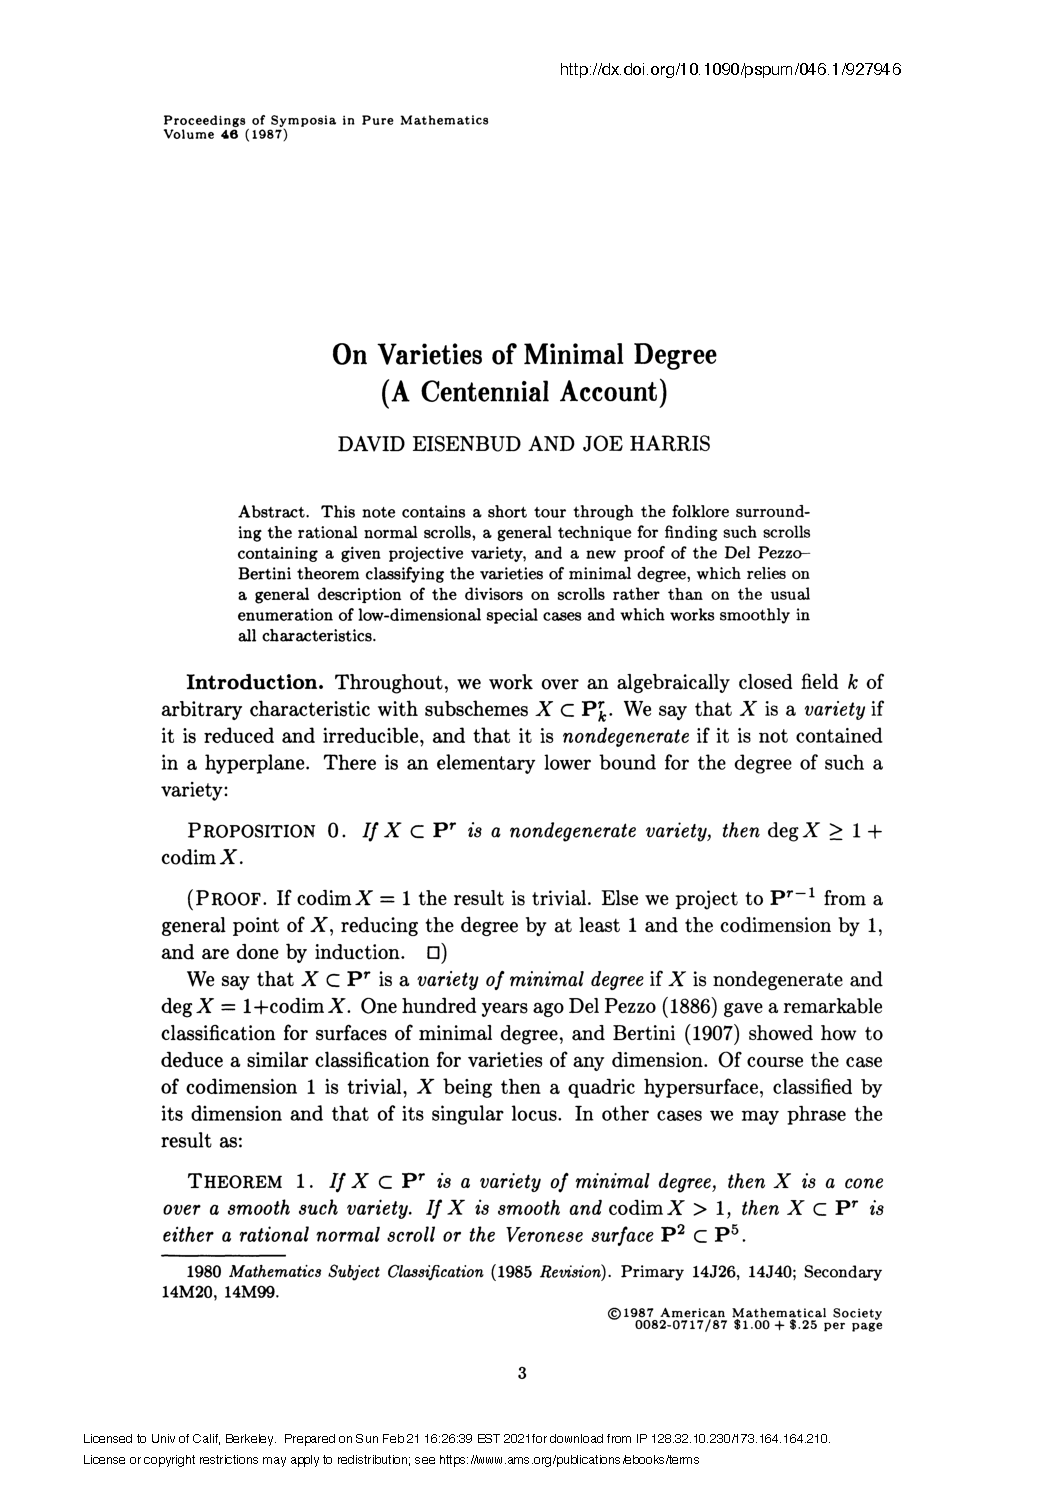
\includepdf[pages=1-11]{Centennial.pdf}
\makeatletter \def\@biblabel#1{\ignorespaces} \makeatother
\bibliographystyle{msribib}
\bibliography{slag}

%% EXPLANATIONS:

% f and n
% some authors have all works collected at the end

\begingroup
%\catcode`\^\active
%if ^ is followed by 
% 1:  print f, gobble the following ^ and the next character
% 0:  print n, gobble the following ^
% any other letter: normal subscript
%\makeatletter
%\def^#1{\ifx1#1f\expandafter\@gobbletwo\else
%        \ifx0#1n\expandafter\expandafter\expandafter\@gobble
%        \else\sp{#1}\fi\fi}
%\makeatother
\let\moreadhoc\relax
\def\indexintro{%An author's cited works appear at the end of the
%author's entry; for conventions
%see the List of Citations on page~\pageref{loc}.  
%\smallbreak\noindent
%The letter `f' after a page number indicates a figure, `n' a footnote.
}
\printindex[gen]
\endgroup % end of \catcode
%requires makeindex

\end{document}


